%%%%%%%%%%%%%%%%%%%%%%%%%%%%%%%%%%%%%%%%%
% Thesis Project
%%%%%%%%%%%%%%%%%%%%%%%%%%%%%%%%%%%%%%%%%

\documentclass[
    b5paper,        % Page size
    fontsize=8.5pt,  % Base font size
    twoside=true,  % Use different layouts for even and odd pages (in particular, if twoside=true, the margin column will be always on the outside)
	open=right, % If twoside=true, uncomment this to force new chapters to start on any page, not only on right (odd) pages
	%chapterentrydots=true, % Uncomment to output dots from the chapter name to the page number in the table of contents
	numbers=noenddot, % Comment to output dots after chapter numbers; the most common values for this option are: enddot, noenddot and auto (see the KOMAScript documentation for an in-depth explanation)
]{kaobook}

%----------------------------------------------------------------------------------------
%	PACKAGES AND OTHER DOCUMENT CONFIGURATIONS
%----------------------------------------------------------------------------------------

% Text encoding
% \usepackage[utf8]{inputenc}
\usepackage{siunitx}

% Choose the language
\ifxetexorluatex
	\usepackage{polyglossia}
	\setmainlanguage{english}
\else
	\usepackage[english]{babel} % Load characters and hyphenation
\fi
\usepackage[english=british]{csquotes}	% English quotes

% Use of book information
\usepackage{authoraftertitle}

% Font
\usepackage{libertine}
\newcommand{\libertineNormal}{\normalfont}
\newcommand{\libertineBold}{\normalfont\bfseries}
\newcommand{\libertineNormalCapital}{\normalfont\scshape}
\newcommand{\libertineBoldCapital}{\normalfont\bfseries\scshape}

% Alignment within the page
% \usepackage[usestackEOL]{stackengine}

% Load packages for testing
\usepackage{blindtext}      % Print text without any meaning for testing purposes
%\usepackage{showframe}     % Uncomment to show boxes around the text area, margin, header and footer
%\usepackage{showlabels}    % Uncomment to output the content of \label commands to the document where they are used

% Load the bibliography package
\usepackage{kaobiblio}
\addbibresource{references.bib}       % Bibliography file
\addbibresource{main.bib} 

% Load mathematical packages for theorems and related environments
\usepackage[framed=true]{kaotheorems}

% Load the package for hyperreferences
\usepackage{kaorefs}

% Tables
\usepackage{pdflscape}
\usepackage{rotating}
\usepackage{tabularx}

% Letter spacing
\usepackage{microtype}

% Test
\usepackage{lipsum} 

% Colors
\usepackage{xcolor}

% Hyperref
\usepackage{xurl}
\usepackage{hyperref}

% Variable parameter parsing
\usepackage{xparse}             % http://ctan.org/pkg/xparse
\usepackage{ifmtarg}            % http://ctan.org/pkg/ifmtarg

% Big first letter, emulating IEEE template
\usepackage{lettrine}

% Horizontal lines
\newcommand{\horizontalrule}[2]{\par
  \vspace*{\dimexpr-\parskip-\baselineskip+#1}
  \noindent\rule{\linewidth}{0.2mm}\par
  \vspace*{\dimexpr-\parskip-.5\baselineskip+#2}}

% Control of odd pages
% \usepackage{everypage}
\usepackage[strict]{changepage}

\newcommand{\oddCoverChapter}{\ifoddpage \afterpage{\thispagestyle{empty}\null\newpage} \else \fi}
\newcommand{\oddChapter}{\ifoddpage \else \afterpage{\thispagestyle{empty}\null\newpage} \fi}
\newcommand{\blankPage}{\thispagestyle{empty}\null\newpage}

% Dedication
\newenvironment{starting_phrase}
  {%\clearpage                  % We want a new page          %% I commented this
   \thispagestyle{empty}        % No header and footer
   \vspace*{\stretch{1}}        % Some space at the top
   %\itshape                    % The text is in italics
   \large
   \raggedleft                  % Flush to the right margin
  }
  {\par % end the paragraph
   \vspace{\stretch{3}}         % Space at bottom is three times that at the top
   \normalsize
   % \clearpage                   % Finish off the page
  }

% Book information
\newcommand{\titleEnglish}{New tools for modelling sensor data}
\newcommand{\titleSpanish}{Nuevas herramientas para la modelización de datos procedentes de sensores}
\newcommand{\authorship}{Alfonso López Ruiz}
\newcommand{\mainSupervisor}{Dr. Francisco Ramón Feito Higueruela}
\newcommand{\secondSupervisor}{Dr. Carlos Javier Ogayar Anguita}
\newcommand{\bookPurpose}{PhD Dissertation}
\newcommand{\dateDissertation}{May 2023}
\newcommand{\dateDissertationSpanish}{mayo de 2023}
\newcommand{\department}{Departamento de Informática}
\newcommand{\polytechnicSchool}{Escuela Politécnica Superior de Jaén}
\newcommand{\university}{Universidad de Jaén}

% Chapter title
\newcommand{\prefaceChapterTitle}[4]{
    \noindent\huge
    \libertineNormalCapital
    \textls[#4]{#1}  
    \horizontalrule{#2pt}{#3pt}
}

% Symbols
\usepackage{amsmath}
\usepackage{amssymb}
\usepackage{pifont}
\newcommand{\cmark}{\ding{51}}%
\newcommand{\xmark}{\ding{55}}%

% Debug rare characters
%\DeclareUnicodeCharacter{2121}{I~AM~HERE!!!!}

% Spacing
\newcommand{\minorSpacing}{\vspace{1mm}}

% Colors
\definecolor{redThesis}{HTML}{ba3132}
\definecolor{darkGray}{HTML}{777777}

% Bibliography
\bibliography{references}

% Background images
\usepackage{tikz}
\usepackage{wrapfig}

% Math values %
\usepackage{commath}
\newcommand*{\R}{\mathbb{R}}
\DeclareMathOperator*{\argmin}{argmin}
\DeclareMathOperator*{\argmax}{argmax}
\DeclareMathOperator*{\atan}{atan}
\DeclareMathOperator*{\acos}{acos}
\DeclareMathOperator*{\asin}{asin}
\DeclareMathOperator*{\dis}{d}
\newcommand*\BitAnd{\mathbin{\&}}
\newcommand*\BitOr{\mathbin{|}}
\newcommand*\ShiftLeft{\ll}
\newcommand*\ShiftRight{\gg}
\newcommand*\BitNeg{\ensuremath{\mathord{\sim}}}
\newcommand\inv[1]{#1\raisebox{1.15ex}{$\scriptscriptstyle-\!1$}}
\newcommand\numberthis{\addtocounter{equation}{1}\tag{\theequation}}

% Images with comments within the image %
\newcommand{\imageannotated}[5]{
    \begin{tikzpicture}
        \draw (0, 0) node[inner sep=0] {\includegraphics[width=\textwidth]{#1}};
        \draw (#3, #4) node[text=#5] {#2};
    \end{tikzpicture}
}

\graphicspath{{images/}} % Paths in which to look for images

\makeindex[columns=3, title=Alphabetical Index, intoc] % Make LaTeX produce the files required to compile the index

\makeglossaries             % Make LaTeX produce the files required to compile the glossary
% \newglossaryentry{Remote sensing}{
% 	name=Remote sensing,
% 	description={refers to non-contact techniques that allow recording data about objects' surfaces.}
% }

% Glossary entries (used in text with e.g. \acrfull{fpsLabel} or \acrshort{fpsLabel})
\newacronym[longplural={Airborne Laser Scanning}]{als}{ALS}{Airborne Laser Scanning}
\newacronym[longplural={Advanced Very High-Resolution Radiometer}]{avhrr}{AVHRR-3}{Advanced Very High-Resolution Radiometer}
\newacronym[longplural={Artificial Intelligence}]{ai}{AI}{Artificial Intelligence}
\newacronym[longplural={Artificial Neural Network}]{ann}{ANN}{Artificial Neural Network}
\newacronym[longplural={Average Accuracy}]{aa}{AA}{Average Accuracy}
\newacronym[longplural={Axis-Aligned Bounding Box}]{aabb}{AABB}{Axis-Aligned Bounding Box}
\newacronym[longplural={Back-Projection MRAE}]{bpmrae}{BPMRAE}{Back-Projection MRAE}
\newacronym[longplural={Bidirectional Reflectance Distribution Function}]{brdf}{BRDF}{Bidirectional Reflectance Distribution Function}
\newacronym[longplural={Bidirectional Scatter Distribution Function}]{bsdf}{BSDF}{Bidirectional Scatter Distribution Function}
\newacronym[longplural={Bidirectional Scattering Surface Distribution Function}]{bssdf}{BSSDF}{Bidirectional Scattering Surface Distribution Function}
\newacronym[longplural={Backpack-mounted Mobile LiDAR Scanning}]{bmmls}{BMMLS}{Backpack-mounted Mobile LiDAR Scanning}
\newacronym[longplural={Boundary Volume Hierarchy}]{bvh}{BVH}{Boundary Volume Hierarchy}
\newacronym[longplural={Building Information Modelling}]{bim}{BIM}{Building Information Modelling}
\newacronym[longplural={Bundle Adjustment}]{ba}{BA}{Bundle Adjustment}
\newacronym[longplural={Central Processing Unit}]{cpu}{CPU}{Central Processing Unit}
\newacronym[longplural={Computational Geometry Algorithms Library}]{cgal}{CGAL}{Computational Geometry Algorithms Library}
\newacronym[longplural={China–Brazil Earth Resources Satellite}]{cbers}{CBERS}{China–Brazil Earth Resources Satellite}
\newacronym[longplural={Charge-coupled Devices}]{ccd}{CCD}{Charge-coupled Devices}
\newacronym[longplural={Classic Monte Carlo}]{cmc}{CMC}{Classic Monte Carlo}
\newacronym[longplural={Competitive Adaptive Reweighted Sampling}]{cars}{CARS}{Competitive Adaptive Reweighted Sampling}
\newacronym[longplural={Complementary Metal-Oxide}]{cmos}{CMOS}{Complementary Metal-Oxide}
\newacronym[longplural={Computer-aided Design}]{cad}{CAD}{Computer-aided Design}
\newacronym[longplural={Computer Graphics}]{cg}{CG}{Computer Graphics}
\newacronym[longplural={Constrained Energy Minimization}]{cem}{CEM}{Constrained Energy Minimization}
\newacronym[longplural={Control Point}]{cp}{CP}{Control Point}
\newacronym[longplural={Convolutional Autoencoder}]{cnn-ae}{CNN-AE}{Convolutional Autoencoder}
\newacronym[longplural={Convolutional Neural Network}]{cnn}{CNN}{Convolutional Neural Network}
\newacronym[longplural={Correlation Coefficient}]{cc}{CC}{Correlation Coefficient}
\newacronym[longplural={Cross-Correlogram Spectral Matching}]{ccsm}{CCSM}{Cross-Correlogram Spectral Matching}
\newacronym[longplural={Compute Unified Device Architecture}]{cuda}{CUDA}{Compute Unified Device Architecture}
\newacronym[longplural={Deep Learning}]{dl}{DL}{Deep Learning}
\newacronym[longplural={Dice Spectral Similarity Coefficient}]{dssc}{DSSC}{Dice Spectral Similarity Coefficient}
\newacronym[longplural={Digital Elevation Model}]{dem}{DEM}{Digital Elevation Model}
\newacronym[longplural={Digital Surface Model}]{dsm}{DSM}{Digital Surface Model}
\newacronym[longplural={Digital Terrain Model}]{dtm}{DTM}{Digital Terrain Model}
\newacronym[longplural={Digital Number}]{dn}{DN}{Digital Number}
\newacronym[longplural={Divide and Conquer}]{d&c}{D\&C}{Divide and Conquer}
\newacronym[longplural={Electromagnetic}]{em}{EM}{Electromagnetic}
\newacronym[longplural={Empirical Line Method}]{elm}{ELM}{Empirical Line Method}
\newacronym[longplural={Enhanced Correlation Coefficient}]{ecc}{ECC}{Enhanced Correlation Coefficient}
\newacronym[longplural={External Orientation Parameters}]{eop}{EOP}{External Orientation Parameters}
\newacronym[longplural={Factor Analysis}]{fa}{FA}{Factor Analysis}
\newacronym[longplural={Fast Global Registration}]{fgr}{FGR}{Fast Global Registration}
\newacronym[longplural={Field of View}]{fov}{FOV}{Field of View}
\newacronym[longplural={Focal Plane Array}]{fpa}{FPA}{Focal Plane Array}
\newacronym[longplural={Frames Per Second}]{fps}{FPS}{Frames Per Second}
\newacronym[longplural={Generative Adversarial Network}]{gan}{GAN}{Generative Adversarial Network}
\newacronym[longplural={Geographic Information System}]{gis}{GIS}{Geographic Information System}
\newacronym[longplural={Global Navigation Satellite System}]{gnss}{GNSS}{Global Navigation Satellite System}
\newacronym[longplural={Global Positioning System}]{gps}{GPS}{Global Positioning System}
\newacronym[longplural={General-Purpose Computing on Graphics Processing Units}]{gpgpu}{GPGPU}{General-Purpose Computing on Graphics Processing Units}
\newacronym[longplural={Gradient Descent}]{gd}{GD}{Gradient Descent}
\newacronym[longplural={Graphics Processing Unit}]{gpu}{GPU}{Graphics Processing Unit}
\newacronym[longplural={Graphical User Interface}]{gui}{GUI}{Graphical User Interface}
\newacronym[longplural={Ground Control Points}]{gcp}{GCP}{Ground Control Points}
\newacronym[longplural={Graphic Processing Cluster}]{gpc}{GPC}{Graphic Processing Cluster}
\newacronym[longplural={Genetic Algorithm}]{ga}{GA}{Genetic Algorithm}
\newacronym[longplural={OpenGL Shading Language}]{glsl}{GLSL}{OpenGL Shading Language}
\newacronym[longplural={Ground Sampling Distance}]{gsd}{GSD}{Ground Sampling Distance}
\newacronym[longplural={Hemispherical-Directional Reflectance Function}]{hdrf}{HDRF}{Hemispherical-Directional Reflectance Function}
\newacronym[longplural={High-Quality Shading}]{hqs}{HQS}{High-Quality Shading}
\newacronym[longplural={Hyperspectral Imaging}]{hsi}{HSI}{Hyperspectral Imaging}
\newacronym[longplural={Independent Component Analysis}]{ica}{ICA}{Independent Component Analysis}
\newacronym[longplural={Inertial Measurement Unit}]{imu}{IMU}{Inertial Measurement Unit}
\newacronym[longplural={Infrared Thermal Imaging}]{ir}{IR}{Infrared Thermal Imaging}
\newacronym[longplural={Interferometric Synthetic Aperture Radar}]{insar}{InSAR}{Interferometric Synthetic Aperture Radar}
\newacronym[longplural={Iterative Closest Point}]{icp}{ICP}{Iterative Closest Point}
\newacronym[longplural={Joint Photographic Experts Group}]{jpeg}{JPEG}{Joint Photographic Experts Group}
\newacronym[longplural={$k$-Nearest Neighbours}]{knn}{KNN}{$k$-Nearest Neighbours}
\newacronym[longplural={Kumar–Johnson Spectral Similarity Coefficient}]{kjssc}{KJSSC}{Kumar–Johnson Spectral Similarity Coefficient}
\newacronym[longplural={LASer}]{las}{LAS}{LASer}
\newacronym[longplural={Layered Point Clouds}]{lpc}{LPC}{Layered Point Clouds}
\newacronym[longplural={Leaf Area Index}]{lai}{LAI}{Leaf Area Index}
\newacronym[longplural={Least Discriminant Analysis}]{lda}{LDA}{Least Discriminant Analysis}
\newacronym[longplural={Least-Square Method}]{lsm}{LSM}{Least-Square Method}
\newacronym[longplural={Level of Accuracy}]{loa}{LOA}{Level of Accuracy}
\newacronym[longplural={Level of Detail}]{lod}{LOD}{Level of Detail}
\newacronym[longplural={Level of Overlap}]{loo}{LOO}{Level of Overlap}
\newacronym[longplural={Level of Coverage}]{loc}{LOC}{Level of Coverage}
\newacronym[longplural={Light Detection and Ranging}]{lidar}{LiDAR}{Light Detection and Ranging}
\newacronym[longplural={Linear Mixture Models}]{lmm}{LMM}{Linear Mixture Models}
\newacronym[longplural={Local Search}]{ls}{LS}{Local Search}
\newacronym[longplural={Long Short-Term Memory}]{lstm}{LSTM}{Long Short-Term Memory}
\newacronym[longplural={Long-wave Infrared}]{lwir}{LWIR}{Long-wave Infrared}
\newacronym[longplural={Long-wave}]{lw}{LW}{Long-wave}
\newacronym[longplural={Machine Learning}]{ml}{ML}{Machine Learning}
\newacronym[longplural={Maximum Likelihood Sample Consensus}]{mlsac}{MLSAC}{Maximum Likelihood Sample Consensus}
\newacronym[longplural={Mean Square Error}]{mse}{MSE}{Mean Square Error}
\newacronym[longplural={Mean Absolute Error}]{mae}{MAE}{Mean Absolute Error}
\newacronym[longplural={Mean Relative Absolute Error}]{mrae}{MRAE}{Mean Relative Absolute Error}
\newacronym[longplural={Mid-wave Infrared}]{mwir}{MWIR}{Mid-wave Infrared}
\newacronym[longplural={Mixture-Tuned Matching Filtering Technique}]{mtmf}{MTMF}{Mixture-Tuned Matching Filtering}
\newacronym[longplural={Mobile Laser Scanner}]{mls}{MLS}{Mobile Laser Scanner}
\newacronym[longplural={Mobile Mapping Systems}]{mms}{MMS}{Mobile Mapping Systems}
\newacronym[longplural={Multilayer Perceptron}]{mlp}{MLP}{Multilayer Perceptron}
\newacronym[longplural={Multi-View Stereo}]{mvs}{MVS}{Multi-View Stereo}
\newacronym[longplural={Multiple End-member Spectral Mixture Analysis}]{mesma}{MESMA}{Multiple End-member Spectral Mixture Analysis}
\newacronym[longplural={Near-Infrared}]{nir}{NIR}{Near-Infrared}
\newacronym[longplural={Next Best View}]{nbv}{NBV}{Next Best View}
\newacronym[longplural={Nonnegative Matrix Factorization}]{nnmf}{NNMF}{Nonnegative Matrix Factorization}
\newacronym[longplural={Normalized difference vegetation index}]{ndvi}{NDVI}{Normalized difference vegetation index}
\newacronym[longplural={Object-Oriented Bounding Box}]{oobb}{OOBB}{Object-Oriented Bounding Box}
\newacronym[longplural={Open Source Computer Vision Library}]{opencv}{OpenCV}{Open Source Computer Vision Library}
\newacronym[longplural={Operational Land Imager}]{oli2}{OLI-2}{Operational Land Imager}
\newacronym[longplural={Open Graphics Library}]{opengl}{OpenGL}{Open Graphics Library}
\newacronym[longplural={Open Multi-Processing}]{openmp}{OpenMP}{Open Multi-Processing}
\newacronym[longplural={Operative System}]{os}{OS}{Operative System}
\newacronym[longplural={Oriented FAST and rotated BRIEF}]{orb}{ORB}{Oriented FAST and rotated BRIEF}
\newacronym[longplural={Overall Accuracy}]{oa}{OA}{Overall Accuracy}
\newacronym[longplural={Partially Least Square}]{pls}{PLS}{Partially Least Square}
\newacronym[longplural={Partial Least-Square Discriminant Analysis}]{plsda}{PLS-DA}{Partial Least-Square Discriminant Analysis}
\newacronym[longplural={Particle Swarm Optimization}]{pso}{PSO}{Particle Swarm Optimization}
\newacronym[longplural={Peak Signal-to-Noise Ratio}]{psnr}{PSNR}{Peak Signal-to-Noise Ratio}
\newacronym[longplural={Perspective n Point}]{pnp}{PnP}{Perspective n Point}
\newacronym[longplural={Physically-based Rendering}]{pbr}{PBR}{Physically-based Rendering}
\newacronym[longplural={Planning for Scanning}]{p4s}{P4S}{Planning for Scanning}
\newacronym[longplural={Point Cloud Compression}]{pcc}{PCC}{Point Cloud Compression}
\newacronym[longplural={Point Cloud Library}]{pcl}{PCL}{Point Cloud Library}
\newacronym[longplural={Polygon File Format}]{ply}{PLY}{Polygon File Format}
\newacronym[longplural={Precision Agriculture}]{pa}{PA}{Precision Agriculture}
\newacronym[longplural={Precision Viticulture}]{pv}{PV}{Precision Viticulture}
\newacronym[longplural={Principal Component Analysis}]{pca}{PCA}{Principal Component Analysis}
\newacronym[longplural={Quasi-Monte Carlo}]{qmc}{QMC}{Quasi-Monte Carlo}
\newacronym[longplural={Radial Basis Function}]{rbf}{RBF}{Radial Basis Function}
\newacronym[longplural={Radiance Invariant Feature Transform}]{rift}{RIFT}{Radiance Invariant Feature Transform}
\newacronym[longplural={Radiometric Joint Photographic Experts Group}]{rjpeg}{RJPEG}{Radiometric Joint Photographic Experts Group}
\newacronym[longplural={Random Forest}]{rf}{RF}{Random Forest}
\newacronym[longplural={Random Sample Consensus}]{ransac}{RANSAC}{Random Sample Consensus}
\newacronym[longplural={Real-Time Kinematic}]{rtk}{RTK}{Real-Time Kinematic}
\newacronym[longplural={Red, Green, Blue}]{rgb}{RGB}{Red, Green, Blue}
\newacronym[longplural={RGB-Depth}]{rgbd}{RGB-D}{RGB-Depth}
\newacronym[longplural={Rectified Linear Unit}]{relu}{ReLU}{Rectified Linear Unit}
\newacronym[longplural={Red-Edge}]{reg}{REG}{Red-Edge}
\newacronym[longplural={Remote Sensing}]{rs}{RS}{Remote Sensing}
\newacronym[longplural={Root Mean Square Error}]{rmse}{RMSE}{Root Mean Square Error}
\newacronym[longplural={Scale-Invariant Feature Transform}]{sift}{SIFT}{Scale-Invariant Feature Transform}
\newacronym[longplural={Simulated Annealing}]{sa}{SA}{Simulated Annealing}
\newacronym[longplural={Speeded-Up Robust Features}]{surf}{SURF}{Speeded-Up Robust Features}
\newacronym[longplural={Structure from Motion}]{sfm}{SfM}{Structure from Motion}
\newacronym[longplural={Shader Storage Buffer Object}]{ssbo}{SSBO}{Shader Storage Buffer Object}
\newacronym[longplural={Short-wave Infrared}]{swir}{SWIR}{Short-wave Infrared}
\newacronym[longplural={Signal-to-Noise Ratio}]{snr}{SNR}{Signal-to-Noise Ratio}
\newacronym[longplural={Singular Value Decomposition}]{svd}{SVD}{Singular Value Decomposition}
\newacronym[longplural={Space Filling Curve}]{sfc}{SFC}{Space Filling Curve}
\newacronym[longplural={Spectral Angle Mapper}]{sam}{SAM}{Spectral Angle Mapper}
\newacronym[longplural={Spectral Gradient Angle}]{sga}{SGA}{Spectral Gradient Angle}
\newacronym[longplural={Spectral Correlation Angle}]{sca}{SCA}{Spectral Correlation Angle}
\newacronym[longplural={Spectral Correlation Matching}]{scm}{SCM}{Spectral Correlation Matching}
\newacronym[longplural={Spectral Information Divergence}]{sid}{SID}{Spectral Information Divergence}
\newacronym[longplural={Stack-based Representation}]{sbr}{SBR}{Stack-based Representation}
\newacronym[longplural={Standard Normal Variate}]{snv}{SNV}{Standard Normal Variate}
\newacronym[longplural={Successive Projection Algorithm}]{spa}{SPA}{Successive Projection Algorithm}
\newacronym[longplural={Support Vector Machine}]{svm}{SVM}{Support Vector Machine}
\newacronym[longplural={Surface Area Heuristic}]{sah}{SAH}{Surface Area Heuristic}
\newacronym[longplural={Tabu Search}]{ts}{TS}{Tabu Search}
\newacronym[longplural={Tag Image File Format}]{tiff}{TIFF}{Tag Image File Format}
\newacronym[longplural={Television and Infrared Observation Satellite}]{tiros}{TIROS}{Television and Infrared Observation Satellite}
\newacronym[longplural={Terrestrial Laser Scanning}]{tls}{TLS}{Terrestrial Laser Scanning}
\newacronym[longplural={Thermal Infrared Sensor 2}]{tirs2}{TIRS-2}{Thermal Infrared Sensor 2}
\newacronym[longplural={Thermal Infrared}]{tir}{TIR}{Thermal Infrared}
\newacronym[longplural={Time of Flight}]{tof}{ToF}{Time of Flight}
\newacronym[longplural={T-distributed Stochastic Neighbor Embedding}]{tsne}{t-SNE}{T-distributed Stochastic Neighbor Embedding}
\newacronym[longplural={Two-Dimensional Correlation Spectroscopy}]{2dcs}{2DCS}{Two-Dimensional Correlation Spectroscopy}
\newacronym[longplural={Universal Transverse Mercator}]{utm}{UTM}{Universal Transverse Mercator}
\newacronym[longplural={Ultra High-Definition}]{uhd}{UHD}{Ultra High-Definition}
\newacronym[longplural={Ultraviolet}]{uv}{UV}{Ultraviolet}
\newacronym[longplural={Uniform Manifold Approximation and Projection}]{umap}{UMAP}{Uniform Manifold Approximation and Projection}
\newacronym[longplural={Unmanned Aerial System}]{uas}{UAS}{Unmanned Aerial System}
\newacronym[longplural={Video Random Access Memory}]{vram}{VRAM}{Video Random Access Memory}
\newacronym[longplural={Virtual Reality}]{vr}{VR}{Virtual Reality}
\newacronym[longplural={Visual Simultaneous Localization and Mapping}]{vslam}{VSLAM}{Visual Simultaneous Localization and Mapping}

        % Include the glossary definitions

\makenomenclature           % Make LaTeX produce the files required to compile the nomenclature

% Reset sidenote counter at chapters
%\counterwithin*{sidenote}{chapter}

%----------------------------------------------------------------------------------------

\begin{document}

\frontmatter % Denotes the start of the pre-document content, uses roman numerals

%----------------------------------------------------------------------------------------
%	OPENING PAGE
%----------------------------------------------------------------------------------------

%\makeatletter
%\extratitle{
%	% In the title page, the title is vspaced by 9.5\baselineskip
%	\vspace*{9\baselineskip}
%	\vspace*{\parskip}
%	\begin{center}
%		% In the title page, \huge is set after the komafont for title
%		\usekomafont{title}\huge\@title
%	\end{center}
%}
%\makeatother

%----------------------------------------------------------------------------------------
%	OUTPUT TITLE PAGE AND PREVIOUS
%----------------------------------------------------------------------------------------

% \begin{center}
    \null\vspace{8mm}
    
    \libertineNormalCapital
    {
        \huge 
        \textcolor{redThesis}{
            \textls[30]
            {
                \titleEnglish
            }
        }
    
        \vspace{5mm}
        
        \Large
        \authorship
    }
    
    \vspace{5mm}
    
    \libertineNormal
    {
        \Large 
        A dissertation submitted in partial fulfillment of the\\
        \minorSpacing
        requirements for the degree of Doctor of Philosophy
    }
    
    \vspace{8mm}
    
    {
       \libertineNormalCapital
       \Large 
       Supervisors:\\
    
       \libertineNormal
       \mainSupervisor\\
       \minorSpacing
       \secondSupervisor
    }
    
    \vspace{15mm}
    
    
\includegraphics[width=0.5\textwidth]{images/Uja/UjaPhDBlack.jpg}
    
    \vspace{3mm}
    
    {
        \libertineNormal
        \Large 
        \department\\
        \minorSpacing
        \polytechnicSchool\\
        \minorSpacing
        \university\\
    
        \vspace{12mm}
        \dateDissertation
    }
    
    \libertineNormal
    \newpage
\end{center}
\begin{center}
    \null\vspace{2mm}

    
\includegraphics[width=0.45\textwidth]{images/Uja/UjaPhD.png}
    
    \vspace{5mm}
    
    {
        \libertineNormalCapital
        \LARGE
        \textls[30]
        {
            tesis doctoral
        }

        \libertineNormalCapital
        \Huge 
        \textcolor{redThesis}{
            \textls[20]
            {
                new tools for\\ 
                \vspace{3mm}
                modelling sensor data
            }
        }
    }
    
    \vspace{55mm}

    \raggedleft
    {
       \libertineBoldCapital
       \Large 
       Presentada por:\\

       \vspace{2mm}
       
       \libertineNormalCapital
       \authorship
    }
    
    \vspace{5mm}

    \raggedleft
    {
       \libertineBoldCapital
       \Large 
       Dirigida por:\\

       \vspace{1mm}
    
       \libertineNormalCapital
       \mainSupervisor\\
       \minorSpacing
       \secondSupervisor
    }

    \vspace{6mm}

    \raggedleft
    {
        \libertineNormalCapital
        \Large 
        Jaén, \dateDissertationSpanish
    }
    
    \libertineNormal
    \newpage
\end{center}

%----------------------------------------------------------------------------------------
%	STARTING PHRASE AND COPYRIGHT
%----------------------------------------------------------------------------------------

\blankPage
\begin{starting_phrase}
	I do not know how long he kept on like this, hating to go on, not daring to stop, on, on, until he was tireder than tired. It seemed like all the way to tomorrow and over it to the days beyond.\\
	\flushright -- J. R. R. Tolkien, The Hobbit
\end{starting_phrase}
\newpage
\vspace*{\fill}
\large 
\begin{center}
    \authorship: \titleEnglish, \textcopyright \hspace{1mm} \dateDissertation
\end{center}

%----------------------------------------------------------------------------------------
%	PRESENTATION AND SIGNS
%----------------------------------------------------------------------------------------

\blankPage
\blankPage
\large

\begin{center}
El \textbf{\mainSupervisor}, Catedrático de Universidad, y el \textbf{\secondSupervisor}, Profesor Titular de Universidad del \department \hspace{1mm} de la \university,
\end{center}

\vspace{2cm}

\begin{center}
CERTIFICAN:
\end{center}

\begin{center}
Que la presente memoria, titulada \textbf{\titleSpanish}, ha sido realizada bajo su dirección y autorizan su presentación y defensa para optar al grado de Doctor por la \university \hspace{1mm} con mención de Doctor Internacional.
\end{center}

\vspace{4cm}

\begin{tabularx}{\dimexpr\linewidth}[t]{@{}XX@{}}
    \centering \textbf{\mainSupervisor}\\\department\\\university & 
    \centering \textbf{\secondSupervisor}\\\department\\\university
\end{tabularx}

\vspace{4cm}

\begin{center}
    \textbf{\authorship}\\
    Ingeniero en Informática
\end{center}

\begin{center}
    Jaén, \dateDissertationSpanish
\end{center}

% \begin{flushright}
% 	\textit{Federico Marotta}
% \end{flushright}

\normalsize

%----------------------------------------------------------------------------------------
%	ABSTRACT
%----------------------------------------------------------------------------------------

\pagelayout{smallmargin}
\blankPage
\newpage
\prefaceChapterTitle{abstract}{20}{25}{35}

\normalsize
\libertineNormal
\lipsum[1-4]

\newpage
\prefaceChapterTitle{resumen}{20}{25}{35}

\normalsize
\libertineNormal
\lipsum[1-4]

\oddCoverChapter
\newpage
\prefaceChapterTitle{resumen}{20}{25}{35}

\normalsize
\libertineNormal

El objetivo de esta tesis es desarrollar una metodología capaz de controlar múltiples fuentes de datos, incluyendo imágenes y nubes de puntos 3D, así como capaz de corregir y fusionar dichas fuentes para aplicarlas a la monitorización, predicción y optimización de procesos del mundo real. No obstante, trabajar con datos acquirido mediante sensores en tedioso en muchos aspectos, entre los que se incluye la fase de adquisición, marcado de puntos de control o la clasificación de puntos. Para evitar estas tareas, se propone generar datos sintéticos a partir de escenarios modelados de manera realista, evitando así adquirir tecnología con un elevado coste y construyendo conjuntos de datos de gran tamaño de manera muy eficiente. Además, los modelos de estos escenarios se pueden relacionar con etiquetas semánticas y materiales, entre otras propiedades. A diferencia del etiquetado manual, los conjuntos de datos sintéticos no incluyen información errónea que puede inducir a error a los algoritmos que utilicen dichos datos.

Las imágenes procedentes de teledetección, a pesar de presentar diferencias de intensidad notables, se pueden fusionar maximizando la correlación entre ellas. Esta tesis emplea el algoritmo de registro de imágenes conocido como \textit{Enhanced Correlation Coefficient} para el registro de imágenes multiespectrales, térmicas y en el espectro visible. Después, la proyección de información multiespectral y térmica al 3D se hace transfiriendo estos datos a una nube densa de puntos RGB reconstruida con fotogrametría. El objetivo que se persigue utilizando la proyección en lugar de una reconstrucción directa es obtener nubes de puntos densas y con una geometría precisa a partir de imágenes de muy baja resolución. Ademñas, esta metodología es notablemente más eficiente que la que integra algunas soluciones comerciales. La calidad de los datos radiométricos se garantiza teniendo en cuenta la oclusión, y minimizando la disilimitud entre la agregación de múltiples muestras y éstas mismas.

Por otra parte , los datos hiperespectrales se proyectaron a nubes de puntos voxelizadas (2.5D) mediante una metodología adaptada al escaneo de tipo \textit{push broom}. En primer lugar, se corrige la geometría de las imágenes hiperespectrales y se solapan para componer un ortomosaico. Después, éste se proyecta en una nube voxelizada. Debido al gran volumen del hipercubo resultante, se comprimen los datos radiométricos mediante una representación basada en \textit{stacks}. Finalmente, se renderiza en tiempo real el hipercubo comprimido mediante la construcción de la imagen en múltiples frames, de manera iterativa.
 
En comparación con los datos previos, los datos sintéticos se centran en la tecnología LiDAR. La base de esta simulación es la indexación de escenarios con un alto nivel de detalle mediante estructuras de datos diseñadas para resolver rápidamente intersecciones rayo-triángulo. Sobre esta base, se incluyen errores sistemáticos y aleatorios, tales como puntos anómalos, ruido en la trayectoría del rayo o pérdidas de retornos, entre otros. Además, se generan escenarios procedurales enriquecidos con datos semánticos y materiales, que posibilitan la construcción de grandes conjuntos de datos LiDAR. Los escaneos aéreos y terrestres se parametrizan para poder incluir un amplio número de sensores comerciales. Los escaneos aéreos integran múltiples patrones de escaneo, mientras que la intensidad se calcula utilizando muestras obtenidas con un goniofotómetro, publicadas en una base de datos de BRDFs. Por último, también se contemplan longitudes de onda diferentes en el sensor LiDAR, incluyendo así el escaneo batimétrico, y se simulan múltiples retornos.

Esta tesis concluye mostrando los beneficios de los datos fusionados y generados de manera sintética mediante tres casos de estudio diferentes. La simulación LiDAR se emplea para optimizar el escaneado de edificios mediante búsquedas locales, que mejora las posiciones de escaneo, y algoritmos genéticos, que minimizan el número de escaneos necesarios. Estas metaheurísticas son guiadas por cuatro funciones objetivo que evalúan precisión, cobertura, nivel de detalle y solapamiento de los escaneos propuestos. Después, nubes de puntos térmicas y mapas ortorectificado, también térmicos, se emplean en la identificación de posibles restos enterrados y la reconstrucción de la estructura de un yacimiento arqueológico mal conservado. Se muestra así el potencia de la teledetección para preservar el patrimonio histórico. Finalmente, los datos hiperespectrales se corrigen y transforman para entrenar una red neuronal convolucional con el objetivo de clasificar variedades de vid.

\pagelayout{wide}

%----------------------------------------------------------------------------------------
%	PUBLICATIONS
%----------------------------------------------------------------------------------------

% Parameters: Title, Authors, Journal, Year, DOI, URL, Rest.
\newcommand{\journalPublication}[7]{
    #2, #4. #1. #3, #7. doi: \href{#6}{#5}.
}

% Parameters: Title, Authors, Journal, Year.
\newcommand{\pendingJournalPublication}[3]{
    #2, #3. #1.
}

% Parameters: Title, Authors, Journal, Year, DOI, URL, Location
\newcommand{\conferencePublication}[7]{
    #2, #4. #1. #3, #7. doi: \href{#6}{#5}.
}

\DeclareDocumentCommand{\journalQuartiles}{ m m m o o o o o o }{%
    Journal impact factor: #1. #2 in \textit{#3}\IfNoValueTF{#4}{}{, #4 in \textit{#5}}\IfNoValueTF{#6}{}{, #6 in \textit{#7}}\IfNoValueTF{#8}{.}{, #8 in \textit{#9}.}
}

\newcommand{\conferenceRating}[1]{Conference rating: #1.}

\prefaceChapterTitle{publications}{19}{24}{35}

\normalsize
\libertineNormal
The following work is already published unless indicated otherwise. These are organized into journals and peer-reviewed conferences; the first are sorted according to the JRC quartile and impact factor, while the latter are classified according to the conference rating from GII (Group of Italian Professors of Computer Engineering), GRIN (Group of Italian Professors of Computer Science), and SCIE (Spanish Computer-Science Society):

\begin{itemize}
    \item \textbf{JCR-indexed journals}
    \begin{itemize}[parsep=6pt]
        \item {
            \journalPublication{An optimized approach for generating dense thermal point clouds from UAV-imagery}{\textbf{Alfonso López-Ruiz} and Juan-Manuel Jurado-Rodríguez and Carlos-Javier Ogayar Anguita and Francisco-Ramón Feito-Higueruela}{ISPRS Journal of Photogrammetry and Remote Sensing}{2021}{10.1016/j.isprsjprs.2021.09.022}{https://doi.org/10.1016/j.isprsjprs.2021.09.022}{volume 97, pp. 78-95}

            \journalQuartiles{11.774}{Q1 (1/50)}{Geography, Physical}[Q1 (6/202)][Geosciences, Multidisciplinary]
            }
        \item {
            \journalPublication{Metaheuristics for the optimization of Terrestrial LiDAR set-up}{\textbf{Alfonso López-Ruiz}, Carlos-Javier Ogayar-Anguita, Juan-Manuel Jurado-Rodríguez \& Francisco Ramón Feito}{Automation in Construction}{2023}{10.1016/j.autcon.2022.104675}{https://www.sciencedirect.com/science/article/abs/pii/S0926580522005453}{volume 146, pp. 104675}
            
            \journalQuartiles{10.517}{Q1 (3/68)}{Construction \& Building Technology}[Q1 (1/138)][Civil Engineering]
            }
        \item {
            \journalPublication{A GPU-accelerated framework for simulating LiDAR scanning}{\textbf{Alfonso López-Ruiz} and Carlos-Javier Ogayar-Anguita and Juan-Manuel Jurado Rodríguez and Francisco-Ramón Feito-Higueruela}{IEEE Transactions on Geoscience and Remote Sensing}{2022}{10.1109/tgrs.2022.3165746}{https://doi.org/10.1109/tgrs.2022.3165746}{volume 60, pp. 1-18}

            \journalQuartiles{8.125}{Q1 (29/276)}{Electrical \& Electronic Engineering}[Q1 (5/87)][Geochemistry \& Geophysics][Q1 (4/34)][Remote Sensing][Q1 (5/28)][Imaging Science \& Photographic Technology]
            }
        \item {
            \journalPublication{Remote sensing image fusion on 3D scenarios: A review of applications for agriculture and forestry}{Juan-Manuel Jurado-Rodríguez, \textbf{Alfonso López-Ruiz}, Luís-Filipe Machado-Pádua \& Joaquim-João Sousa-Moreira}{International Journal of Applied Earth Observation and Geoinformation}{2022}{10.1016/j.jag.2022.102856}{https://doi.org/10.1016}{volume 112, pp. 102856}

            \journalQuartiles{7.672}{Q1 (5/34)}{Remote Sensing}
            }
        \item {
            \journalPublication{A framework for registering {UAV}-based imagery for crop-tracking in Precision Agriculture}{\textbf{Alfonso López-Ruiz}, Juan-Manuel Jurado-Rodríguez, Carlos-Javier Ogayar-Anguita \& Francisco-Ramón Feito-Higueruela}{International Journal of Applied Earth Observation and Geoinformation}{2021}{10.1016/j.jag.2020.102274}{https://doi.org/10.1016\%2Fj.jag.2020.102274}{volume 97, pp. 102274}

            \journalQuartiles{7.672}{Q1 (5/34)}{Remote Sensing}
            }
        \item {
            \journalPublication{Efficient generation of occlusion-aware multispectral and thermographic point clouds}{\textbf{Alfonso López-Ruiz}, Carlos-Javier Ogayar-Anguita, Juan-Manuel Jurado-Rodríguez \& Francisco-Ramón Feito-Higueruela}{Computers and Electronics in Agriculture}{2023}{\\10.1016/j.compag.2023.107712}{https://doi.org/10.1016/j.compag.2023.107712}{volume 207, pp. 107712}
            
            \journalQuartiles{6.757}{Q1 (4/59)}{Agriculture, Multidisciplinary}[Q1 (23/112)][Computer Science, Interdisciplinary Applications]
        }
        \item {
            \journalPublication{Generation of hyperspectral point clouds: Mapping, compression and rendering}{\textbf{Alfonso López-Ruiz}, Juan-Manuel Jurado-Rodríguez, Juan-Roberto Jiménez-Pérez \& Francisco-Ramón Feito-Higueruela}{Computer \& Graphics}{2022}{10.1016/j.cag.2022.06.011}{https://doi.org/10.1016/j.cag.2022.06.011}{volume 106, pp. 267-276}

            \journalQuartiles{1.821}{Q3 (68/110)}{Computer Science, Software Engineering}
            }
    \end{itemize}
    \item \textbf{Peer-reviewed conferences}
        \begin{itemize}[parsep=6pt]
        \item {
            \conferencePublication{GPU-based Mapping of Thermal Imagery for Generating 3D Occlusion-Aware Point Clouds}{\textbf{Alfonso López-Ruiz}, Juan-Manuel Jurado-Rodríguez, Carlos-Javier Ogayar-Anguita and Francisco-Ramón Feito-Higueruela}{IGARSS 2022 (2022 IEEE International Geoscience and Remote Sensing Symposium)}{July 17-22, 2022}{10.1109/igarss46834.2022.9884240}{https://doi.org/10.1109\%2Figarss46834.2022.9884240}{Kuala-Lumpur (Malaysia)}

            \conferenceRating{B-, Class 3}
            }
        \item {
            \conferencePublication{Comparison of GPU-based Methods for Handling Point Cloud Occlusion}{\textbf{Alfonso López-Ruiz}, Juan-Manuel Jurado-Rodríguez, Emilio-José Padrón, Carlos-Javier Ogayar-Anguita \& Francisco-Ramón Feito-Higueruela}{2021 Spanish Computer Graphics Conference (CEIG)}{September 22–24 2021}{10.2312/ceig.20211364}{https://diglib.eg.org/handle/10.2312/ceig.20211364}{Málaga (Spain)}
            }
        \item {
            \conferencePublication{A GPU-accelerated LiDAR Sensor for Generating Labelled Datasets}{\textbf{Alfonso López-Ruiz}, Carlos-Javier Ogayar-Anguita \& Francisco-Ramón Feito-Higueruela}{2021 Spanish Computer Graphics Conference (CEIG)}{September 22–24 2021}{10.2312/ceig.20211360q}{https://diglib.eg.org/handle/10.2312/ceig.20211360q}{Málaga (Spain)}
            }
        \item {
            \conferencePublication{Multispectral Registration, Undistortion and Tree Detection for Precision Agriculture}{\textbf{Alfonso López-Ruiz}, Juan-Manuel Jurado-Rodríguez, Carlos-Javier Ogayar-Anguita \& Francisco-Ramón Feito-Higueruela}{2019 Spanish Computer Graphics Conference (CEIG)}{June 26-28 2019}{10.2312/ceig.20191209}{https://https://diglib.eg.org/handle/10.2312/ceig20191209}{San Sebastián (Spain)}
            }
        \end{itemize}
    \item \textbf{Pending publications}
        \begin{itemize}[parsep=6pt]
            \item {
                \pendingJournalPublication{Semantic BRDF-based LiDAR point cloud generation on the GPU}{\textbf{Alfonso López-Ruiz}, Carlos-Javier Ogayar-Anguita, Rafael-Jesús Segura-Sánchez}{2023}
            }
            \item {
                \pendingJournalPublication{Classification of vineyard varieties using UAV hyperspectral imaging}{\textbf{Alfonso López-Ruiz}, Joaquim-João Moreira-de Sousa, Carlos-Javier Ogayar-Anguita \& Francisco-Ramón Feito-Higueruela}{2023}
            }
            \item {
                \pendingJournalPublication{Detection of landscape features with visible and thermal imaging}{Carolina Collado, Carmen Enríquez-Muñoz, \textbf{Alfonso López-Ruiz}, Carlos Enríquez \& Juan-Manuel Jurado-Rodríguez}{2023}
            }
        \end{itemize}
    % \item \textbf{Other publications not directly related or explained}
    %     \begin{itemize}
    %         \item \textbf{JCR-indexed journals}
    %             \begin{itemize}[parsep=6pt]
    %                 \item {
    %                     \journalPublication{Nested spatial data structures for optimal indexing of LiDAR data}{Carlos-Javier Ogayar-Anguita, \textbf{Alfonso, López-Ruiz}, Antonio-Jesús Rueda-Ruiz \& Rafael-Jesús Segura-Sánchez}{ISPRS Journal of Photogrammetry and Remote Sensing}{2023}{10.1016/j.isprsjprs.-\\2022.11.018}{https://www.sciencedirect.com/science/article/abs/pii/S0924271622003112}{volume 195, pp. 287–29}
            
    %                     \journalQuartiles{11.774}{Q1 (1/50)}{Geography, Physical}[Q1 (6/202)][Geosciences, Multidisciplinary]
    %                     }
    %                \item {
    %                     \journalPublication{Reconstruction of tree branching structures from UAV-LiDAR data}{José-Luis Cárdenas-Donoso, \textbf{Alfonso López-Ruiz}, Carlos-Javier Ogayar-Anguita and Francisco-Ramón Feito-Higueruela and Juan-Manuel Jurado-Rodríguez}{Frontiers in Environmental Science}{2022}{10.3389/fenvs.2022.960083}{https://www.frontiersin.org/articles/10.3389/fenvs.2022.960083}{volume 10, pp. 1-15}
            
    %                     \journalQuartiles{5.411}{Q2 (82/279)}{Environmental Sciences}
    %                     }
    %             \end{itemize}
    %         \item \textbf{Peer-reviewed conferences}
    %             \begin{itemize}[parsep=6pt]
    %                 \item {
    %                     \conferencePublication{Modeling and Enhancement of LiDAR Point Clouds from Natural Scenarios}{José-Antonio Collado, \textbf{Alfonso López-Ruiz}, Juan- Roberto Jiménez-Pérez, Lidia-María Ortega-Alvarado, Francisco-Ramón Feito-Higueruela \& Juan-Manuel Jurado-Rodríguez}{Eurographics 2022 (Posters)}{2022}{10.2312/egp.20221016}{https://doi.org/10.2312/egp.20221016}{Reims (France)}

    %                     \conferenceRating{A, Class 2}
    %                 }
    %                 \item {
    %                     \conferencePublication{Guided Modeling of Natural Scenarios: Vegetation and Terrain}{José-Antonio Collado, \textbf{Alfonso López-Ruiz}, Juan- Roberto Jiménez-Pérez, Lidia-María Ortega-Alvarado, Juan-Manuel Jurado-Rodríguez \& Francisco-Ramón Feito-Higueruela}{2022 Spanish Computer Graphics Conference (CEIG)}{2022}{10.2312/ceig.20221144}{https://diglib.eg.org/handle/10.2312/ceig.20221144}{Vic (Spain)}
    %                     }
    %             \end{itemize}
    %     \end{itemize}
\end{itemize}

%----------------------------------------------------------------------------------------
%	ACKNOWLEDGMENTS
%----------------------------------------------------------------------------------------

\newpage
\begin{flushright}
	\textit{\lipsum[1-1]}\\
    \textbf{- Hola}
\end{flushright}

\prefaceChapterTitle{Acknowledgments}{19}{24}{35}

\normalsize
\libertineNormal

\lipsum[1-5]

Finalmente, transmitir mi agradecimiento a la Universidad de Jaén por financiar la realización de esta tesis doctoral así como a Bedrich Benes y al grupo de investigación High Performance Computer Graphics de la Universidad de Purdue por aceptar mi solicitud para realizar mi estancia de investigación con ellos.

%----------------------------------------------------------------------------------------
%	TABLE OF CONTENTS & LIST OF FIGURES/TABLES
%----------------------------------------------------------------------------------------

\begingroup % Local scope for the following commands

% Define the style for the TOC, LOF, and LOT
%\setstretch{1} % Uncomment to modify line spacing in the ToC
%\hypersetup{linkcolor=blue} % Uncomment to set the colour of links in the ToC
\setlength{\textheight}{230\hscale} % Manually adjust the height of the ToC pages

% Turn on compatibility mode for the etoc package
\etocstandarddisplaystyle % "toc display" as if etoc was not loaded
\etocstandardlines % "toc lines as if etoc was not loaded

\tableofcontents % Output the table of contents

\listoffigures % Output the list of figures

% Comment both of the following lines to have the LOF and the LOT on 
% different pages
% \let\cleardoublepage\bigskip
% \let\clearpage\bigskip

\listoftables % Output the list of tables

\listoflstlistings % Output the list of listings

\endgroup

%----------------------------------------------------------------------------------------
%	MAIN BODY
%----------------------------------------------------------------------------------------

\mainmatter % Denotes the start of the main document content, resets page numbering and uses arabic numbers
\setchapterstyle{kao} % Choose the default chapter heading style

%----------------------------------------------------------------------------------------
%	GLOSSARY
%----------------------------------------------------------------------------------------

% The glossary needs to be compiled on the command line with 'makeglossaries main' from the template directory

\pagelayout{smallmargin} 
\setglossarystyle{listgroup} % Set the style of the glossary (see https://en.wikibooks.org/wiki/LaTeX/Glossary for a reference)
\printglossary[title=Acronyms, toctitle=Acronyms] % Output the glossary, 'title' is the chapter heading for the glossary, toctitle is the table of contents heading

%----------------------------------------------------------------------------------------
%	NOMENCLATURE
%----------------------------------------------------------------------------------------

% The nomenclature needs to be compiled on the command line with 'makeindex main.nlo -s nomencl.ist -o main.nls' from the template directory

% \pagelayout{smallmargin}
% \nomenclature{$c$}{Speed of light in a vacuum inertial frame}
\nomenclature{$h$}{Planck constant}

\renewcommand{\nomname}{Notation} % Rename the default 'Nomenclature'
\renewcommand{\nompreamble}{The following are the symbols that will be presented within this document to explain different formulas, ranging from image-based operations to optimization functions. } % Prepend this text to the nomenclature

\printnomenclature % Output the nomenclature

\vspace{1cm}

%{\usekomafont{chapter}Greek Letters with Pronunciations} \\[2ex]
\begin{center}
	\newcommand{\pronounced}[1]{\hspace*{.2em}\small\textit{#1}}
	\begin{tabularx}{\textwidth}{l l}
		\toprule
		Character & Name\\ 
		\midrule
		$\alpha$ & alpha \\
		$\beta$ & beta\\ 
		$\gamma$, $\Gamma$ \\
		\bottomrule
	\end{tabularx} \\[1.5ex]
	Capitals shown are the ones that differ from Roman capitals.
\end{center}
% \pagelayout{margin}

%----------------------------------------------------------------------------------------
%	THESIS
%----------------------------------------------------------------------------------------

%----------------------------------------------------------------------------------------
%	PART I
%----------------------------------------------------------------------------------------

% \oddCoverChapter
% \chapterBackground{figs/chapters/b5/Chapter1_01.png}{figs/chapters/b5/Chapter1_02.png}{Radu Carstean}{Pawn Mate}{Sketchfab}{black}

\blankPage
\partIntro{I}{Introduction and overview}{This section introduces a shallow background of Remote Sensing as well as the aim and objectives of this doctoral dissertation. Then, the state-of-the-art on the fusion and simulation of Remote Sensing data is presented.}

\setchapterpreamble[u]{\margintoc}
\chapter{Introduction}
\labch{intro}

\lettrine[findent=0pt, lines=3]{\textbf{S}}{ }ensing real-world processes help to monitor, predict and optimize the activities that depend on them and therefore act according to the analyzed data. Numerous devices are aimed at this task, which can be at least classified according to the sensing distance, the wavelength interval captured by the device detectors and the data acquisition mechanism, either passive or active. The latter two classifications are based on how a device works as provided by the manufacturer. However, choosing a sensing distance is up to researchers and consumers, depending on their objectives, area of expertise and budget, as well as on the dimensions and environmental conditions of the study area, among other factors. Despite contact-based sensors being implemented nowadays to measure variables such as humidity, temperature or rainfall amount, these require a high degree of maintenance and are more prone to deteriorate under adverse environmental conditions \cite{silva_low-cost_2019, morais_versatile_2021}. Instead of covering large areas, each one of these sensors communicates measurements of very specific locations within and outside a network. The arranged layout, logically and physically, must be carefully designed for intra- and extra-communication involving nodes in different topological levels. Therefore, these technologies have a worse spatial awareness and are more appropriate to cope with real-time, rapid and constant monitoring. 

\marginnote[.1cm]{\textbf{Remote sensing} techniques overcome the spatial limitations of devices that measure data in contact with the target surface and phenomena.} 
Given the cited drawbacks, \textbf{Remote sensing} (\acrshort{rs}) techniques help to mitigate them by acquiring data from remote platforms. \acrshort{rs} refers to the science and art of acquiring information about objects and phenomena without being in contact with them \cite{lillesand_remote_2015}. Similarly to the human eye, data is acquired from the environment in the form of impulses from light stimuli corresponding to some wavelength intervals. At least two components are involved in the reading process: the sensors and the platforms where they are mounted. The first will be the matter of discussion throughout this dissertation, whereas platforms were initially narrowed to satellites. 

\begin{marginfigure}[0cm]
	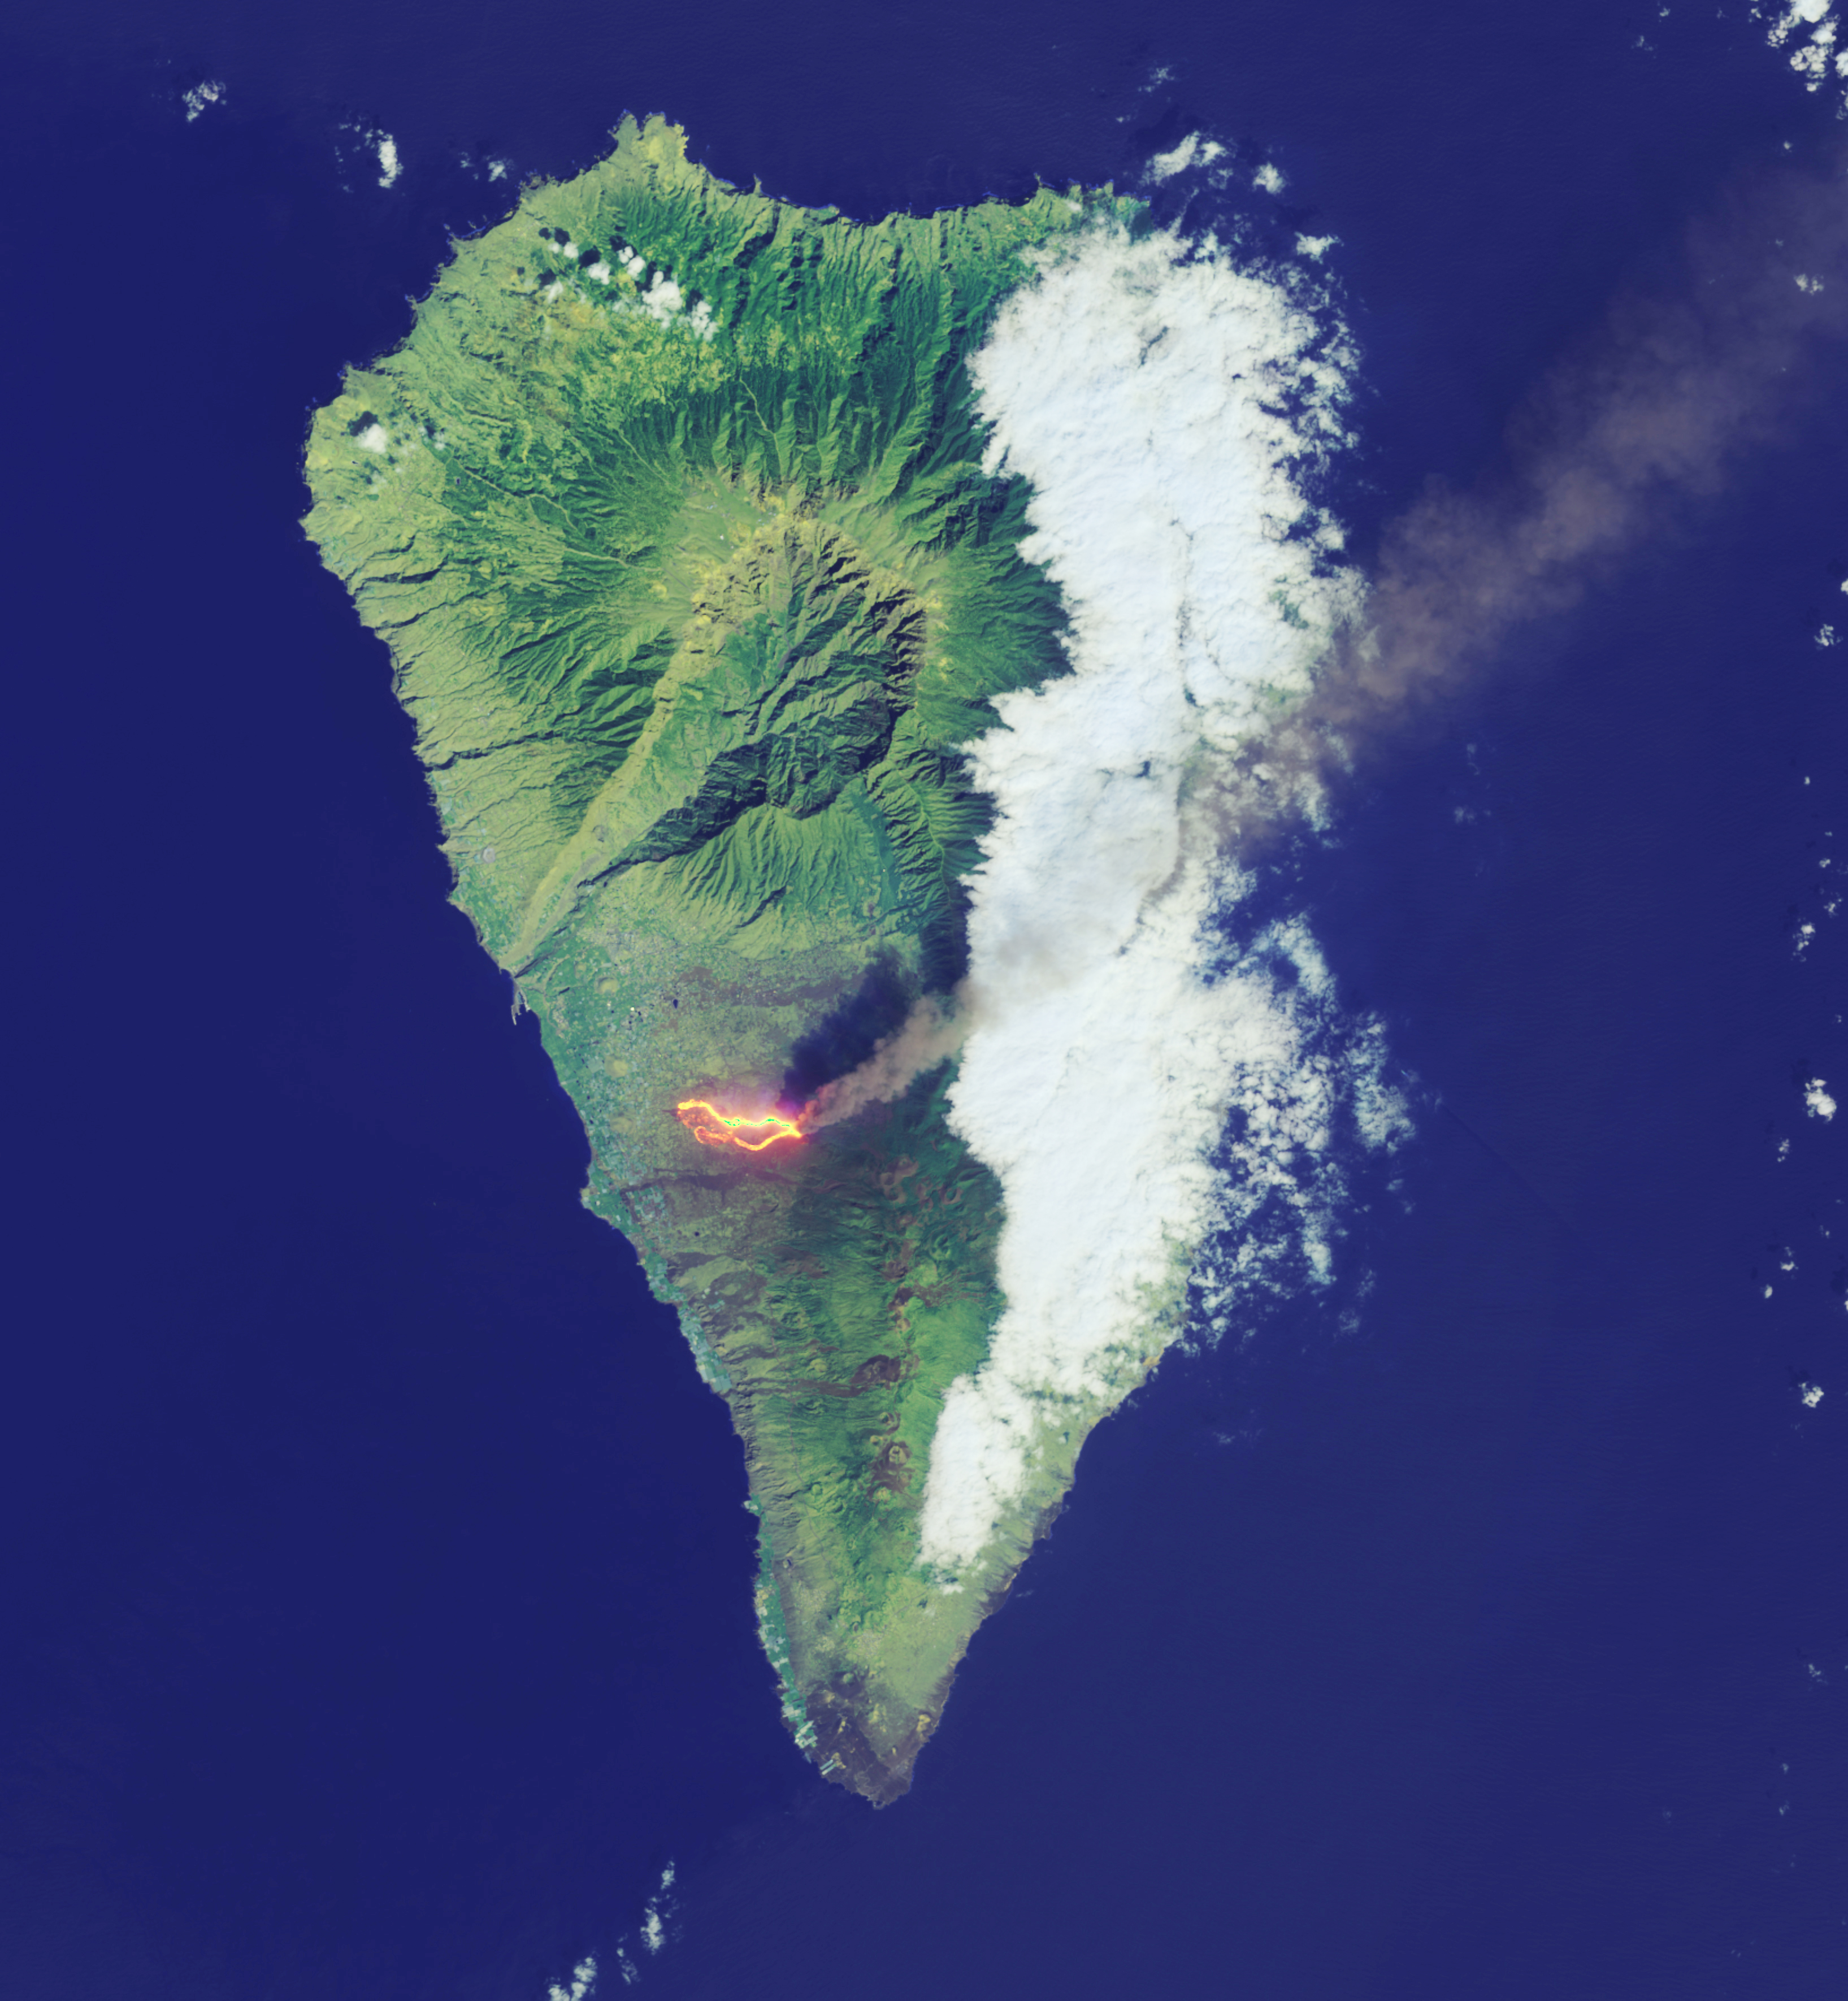
\includegraphics{figs/introduction/landsat8_lapalma.jpg}
	\caption{Cumbre Vieja volcano eruption observed from Landsat-8 \cite{nasa_earth_observatory_lava_2021}.}
	\label{fig:la_palma_landsat8}
\end{marginfigure}
\textbf{Satellite imaging} is better suited for the monitoring of changes over large areas using time series spanned over months and years. These data help to understand the dynamics of human and nature interaction as well as the impact of natural phenomena (Figure \ref{fig:la_palma_landsat8}). Some applications of the large collections of available satellite data are the analysis of land use, deforestation, land changes and urban settlements \cite{asokan_change_2019}. Nevertheless, the spatial resolution and revisit period of non-commercial satellite programmes harden their applicability to fine-grained monitoring tasks. The level of detail (\acrshort{lod}) of these tasks can refer to \textbf{spatial resolution}, \textbf{temporal resolution} or both, which are the main \textbf{limitations} of satellite imaging besides their cost. In spite of the described drawbacks, the use of satellite imagery is on the rise due to the steady reduction of Ground Sampling Distance (\acrshort{gsd}) and low periods for revisiting the same points. 

Figure \ref{fig:scopus_search_platforms} depicts the amount of research devoted to each remote sensing platform. The Scopus searches were the following: $(p_1 \lor p_2 ... \lor p_n) \land (\textit{remote} \hspace{1mm} \land \hspace{1mm} \textit{sensing})$, with $p_i$ being one of the platforms depicted in the legend. 

\begin{figure}[!ht]
	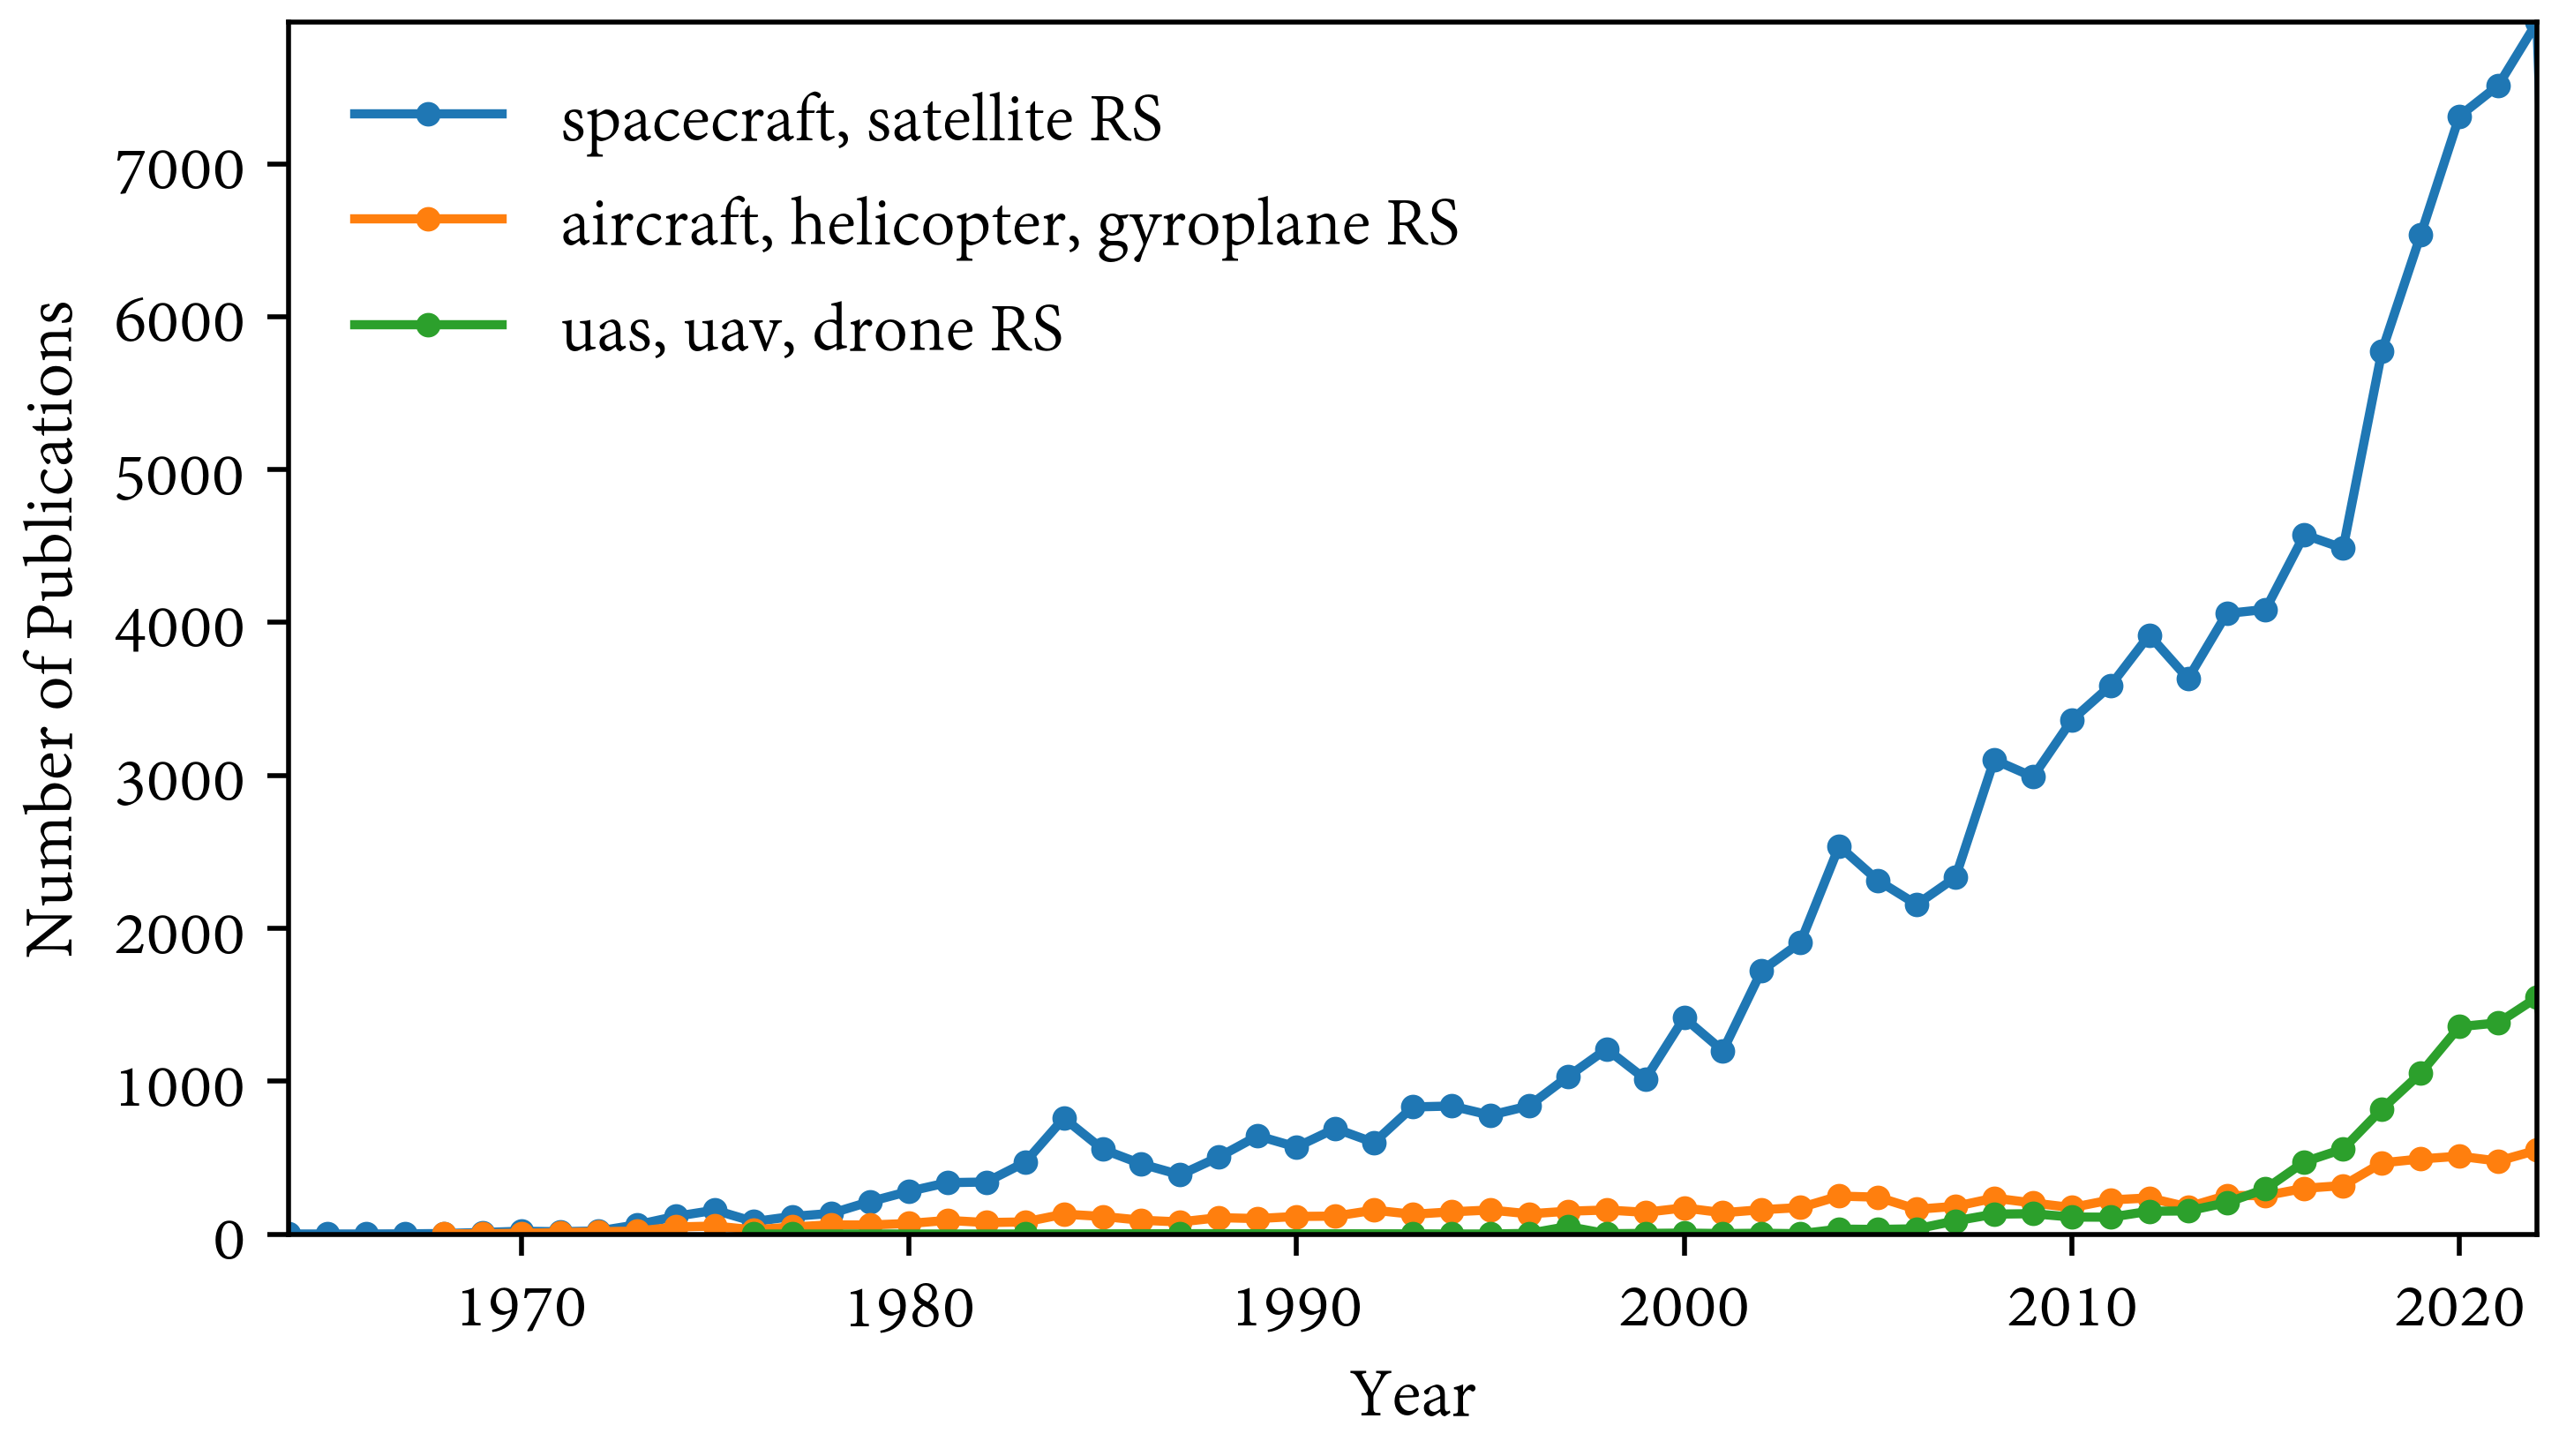
\includegraphics[width=\linewidth]{figs/introduction/platform_timeline.png}
	\caption{Number of manuscripts related to different \acrshort{rs} platforms. }
    \label{fig:scopus_search_platforms}
\end{figure}

However, it was until recently that satellite resolution was restricted by governments. These restrictions as well as the described limitations led to the use of alternative platforms. Besides satellites, \textbf{airborne} (fixed-wing and helicopters), \textbf{Unmanned Aerial Systems} (\acrshort{uas}) (Figure \ref{fig:dji300}) and other \textbf{land platforms} (mobile and static proximal-sensing) are the most frequent \cite{lillesand_remote_2015}. The choice of any of them always involves trade-offs concerning manoeuvrability, land coverage, repeat coverage, spatial resolution, spatial accuracy, cost or field of view (\acrshort{fov}) \cite{toth_remote_2016}. However, \textbf{\acrshort{uas}} have been gaining interest in the last decade as they transitioned from military tools in the early 2000s to easy-to-deploy, small and low-cost systems, thus widening their applicability to civilian activities and research. These platforms range from hand-sized to large aircraft that can be either controlled by human intervention or be partially, even fully, autonomous. Figure \ref{fig:dji300} shows a standard \acrshort{uas} designed by DJI which can carry up to 2.7 \si{\kilo\gram}, with a size of $810 \times 660 \times 430$ \si{\milli\meter}.
\begin{marginfigure}[-3cm]
	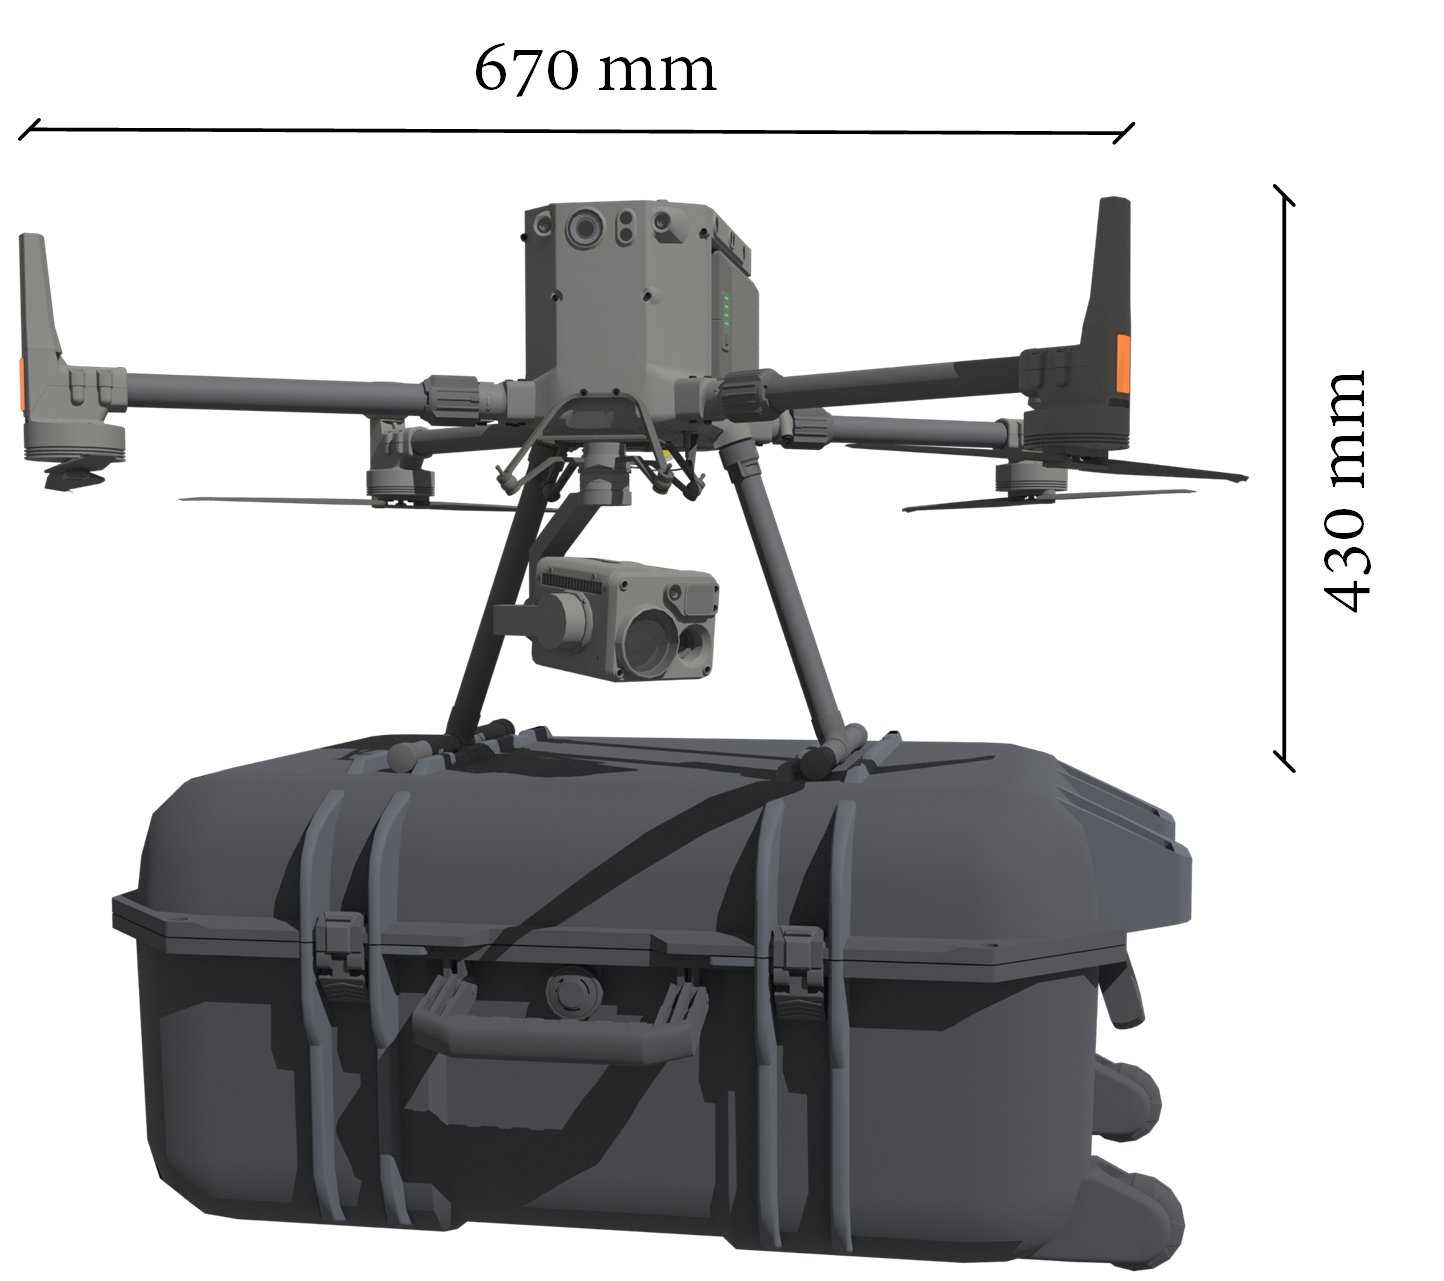
\includegraphics{figs/introduction/dji300.png}
	\caption{Quadcopter Matrice 300 RTK coupled with a dual RGB-thermal sensor (Zenmuse H20T). }
	\label{fig:dji300}
\end{marginfigure}

\begin{figure}[!ht]
	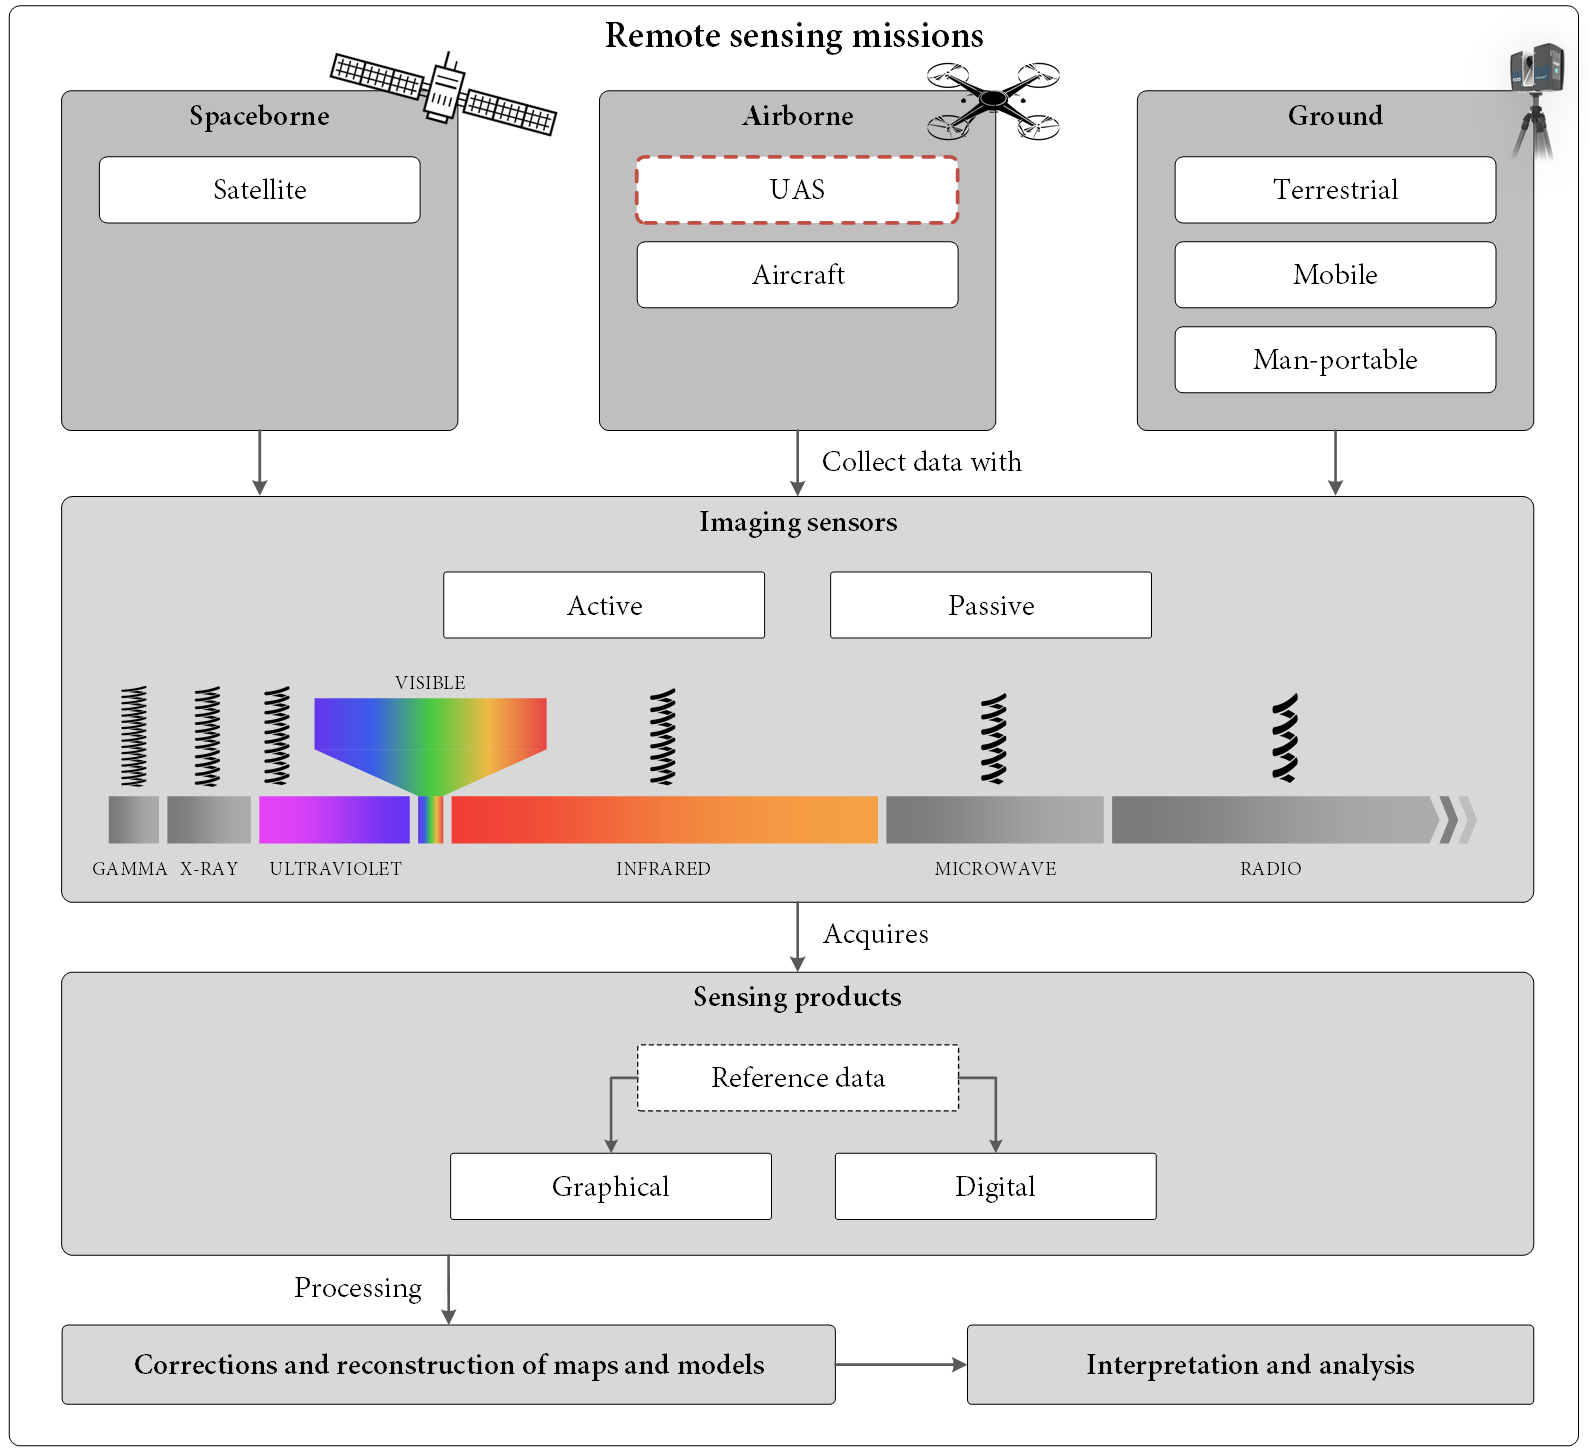
\includegraphics{figs/introduction/introduction_scheme.png}
	\caption{Overall procedure to acquire data with remote sensing platforms and sensors. Firstly, sensors are coupled on spaceborne, airborne and terrestrial vehicles or operated by humans, either by carrying them as a backpack or in hand. Then, sensor products can be grouped into graphical and numerical results, though most of them produce both kinds of data. Finally, the sensing products are processed and interpreted to provide users with valuable analyses. }
    \label{fig:introduction_scheme}
\end{figure}

Therefore, \acrshort{uas}s represent a cost-efficient tool for acquiring high-resolution data. The most common sensors mounted on \acrshort{uas} are cameras and \acrshort{lidar} (Light Detection and Ranging) sensors, with the first comprising a large number of imaging devices. Similarly, these groups also lead to the distinction between passive and active sensors. While the second has both transmitter and receiver components, the first is only aimed at capturing incoming radiance from the scene surfaces. Also, the observations of imaging devices generate 2D images, whereas the immediate results of active sensing are 3D point clouds. Accordingly, the technology involved in \textbf{active sensing} is much more \textbf{prohibitive} than imagers, which have been widespread for the last decades with consumer-grade devices. Still, both kinds of sensors can be applied to the collection of complementary resources. However, the acquisition of multiple high-resolution datasets poses several advantages and drawbacks. 

\marginnote[-1.5cm]{The digitization of assets, processes and systems is greatly helped by reconstructions from sensor data. These allow connecting virtual and physical replicas through a data stream, thus shaping the fundamentals of \textbf{Digital twins}.}
Firstly, observations from multiple sensors can be interpreted as different features that complete a \textbf{knowledge-based system}, with each one providing information within a wavelength range. Furthermore, most of the algorithms aimed at analyzing and drawing conclusions from sensor data benefit from the use of complementary features. The contribution of each one in the extracted conclusions can be adjusted through weights that determine how important are these for the analysis. Unless a large number of features are used, which can lead to the curse of dimensionality problem, it is safe to say that the greater number of features, the better. On the other hand, \textbf{high-resolution data} help to generate \textbf{precise models that are easier to analyze and visualize by human operators}. Denser data also involves denser geometry and reconstructions, thus omitting fewer details of target surfaces and easing the construction of digital models that emulate the Earth's scenarios and processes. 

Different layers of information are ideally noise-free and represented under the same coordinate system. In reality, navigation sensors present small positioning errors that harden the fusion of several layers of information. Despite being small, these are reported as shifts, rotation and scale variations among different sensor data. Furthermore, environmental conditions such as atmospheric composition, wind, temperature or solar radiation can vary from one flight to another and so do the acquired data, even under similar flight plans. These changes not only affect observations performed in a short period of time with different sensors but also time series acquired with previously used tools. Although tedious, variations concerning positioning and orientation errors can be diminished by including reference points measured with sensors of higher precision in easily recognizable image features. Other shortcomings are the noise induced by faulty device detectors, especially for active sensors, unwanted atmospheric particles and surfaces whose bouncing behaviour leads to unreal geometry. Therefore, a system capable of accurately fusing the outcome of every sensor coupled on a \acrshort{uas} is necessary to facilitate the later processing stages and provide reliable conclusions.

Besides the information that can be directly extracted from remotely sensed data, other kinds of information may be required for \textbf{computer vision} tasks. For instance, it would be of great help to distinguish materials and instances in pixels and 3D points. However, these data cannot be inferred from nature without previous knowledge or trained models. Accordingly, one of the main challenges is the \textbf{labelling of large datasets}, which must be performed by human operators \cite{li_image_2021, basu_deepsat_2015} or unsupervised algorithms aimed at transforming and extracting relevant features. None of these methods is perfect and thus can result in spurious labelling data that can mislead the learning algorithms. Hence, the task of building large datasets for training computer vision algorithms is very time-consuming. It comprises acquiring, processing and extracting features with \textbf{considerable computational and human resources}. All these time-consuming stages can be avoided with the existence of publicly available datasets for \acrshort{rs}, motivated by Artificial Intelligence (\acrshort{ai}) algorithms. These cover a wide variety of sensors and spectral wavelengths, but the attached data present the same drawbacks as previously explained. Moreover, these datasets may not comprise areas of interest for case studies that fall out of state-of-the-art trends. 

% Given the cited drawbacks, from which cost and time stand out, datasets could be replaced, at least partially, by synthetically generated information from virtual sensors. The main challenge arises therefore from emulating the sensor mechanism. On the other hand, one advantage is that data acquired from a virtual sensor are linked to digital models without uncertainty. Likewise, digital models are augmented with features that could be directly transferred to the sensing results. These features include the aforementioned semantic annotation or the instances' Id. The most frequently simulated sensors are Radar and \acrshort{lidar} systems, though synthetic images have also been recently generated with the rise of \acrshort{dl} approaches capable of generating new data.  

Given the drawbacks of using real datasets, from which cost and time consumption stand out, \textbf{synthetic information} generated by \textbf{virtual sensors} could be used as a partial or complete replacement. The main challenge lies in emulating the sensor mechanism. However, the process is much less time-consuming and enables adding any kind of knowledge to the sensing results. These are obtained from digital models with no uncertainty, in contrast to what occurs in nature, and they can be enriched with features such as semantic annotations which are later transferred to synthetic datasets. It neither requires acquiring prohibitive sensors such as \acrshort{lidar}, and therefore is also much more cost-efficient. The most frequently simulated sensors are Radar and \acrshort{lidar} systems, but recent advances in Deep Learning (\acrshort{dl}) have made it possible to generate synthetic images as well. 

Sensing products are typically \textbf{transformed} into other \textbf{data representations} that are not provided by the sensor. Accordingly, individual images are not sufficient to interpret the scenario in some contexts. A complete vision of it can be provided by joining images, thus resulting in 2D maps and 3D points calculated by estimating the camera pose and finding features in common among several images. During these transformations, estimated radiometric and geometric properties may be affected by precision loss in the interpolation process. Therefore, it is important to compare the results with other reliable data sources. For instance, \acrshort{lidar} is known to produce highly accurate point clouds, which can be used as a reference to evaluate the quality of point clouds reconstructed from imagery. Similarly, images can serve as reference data for measuring radiometric changes.  

On the other hand, \textbf{large volumes of data are also harder to operate in terms of computing, storage and visualization}. Thousands of images or millions of points can be hardly operated in commodity hardware due to the required storage and computing capabilities. However, current trends in informatics have favoured the proliferation of personal and professional computers with large storage capacity, more efficient access to data and great multi-threading capabilities. The latter can be performed over the Central Processing Unit (\acrshort{cpu}), whose trend is to increase the number of cores, and the Graphic Processing Unit (\acrshort{gpu}), composed of millions of units that can massively solve small tasks and cooperate among small thread groups. Chapter \ref{sec:fundamentals_rs} delves into the most common data formats in \acrshort{rs}; at this moment, it is enough to think of data as large volumes of digital numbers (\acrshort{dn}). Despite large storage being inexpensive nowadays, challenges such as the partial retrieval of information remain, especially for interactive applications with high data throughput \cite{bejar-martos_strategies_2022, ogayar-anguita_nested_2023}. 

\begin{marginfigure}[-.5cm]
	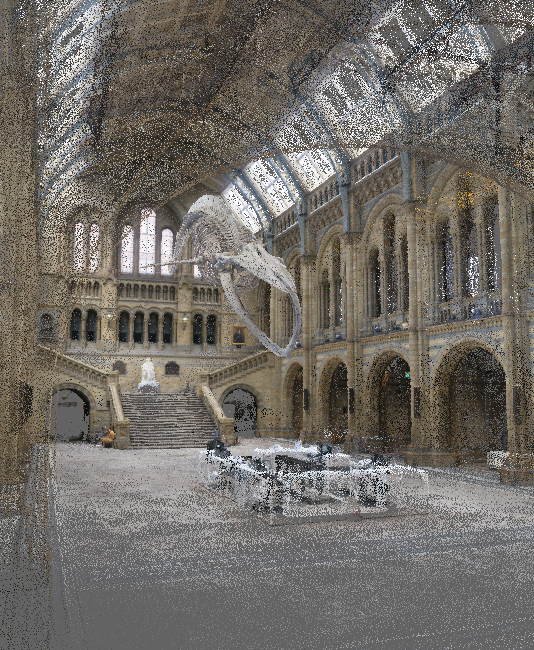
\includegraphics{figs/introduction/hintze.png}
	\caption{Point cloud with 2.4M points, reconstructed using 900 images from the Hintze Hall (Model uploaded by \textit{Thomas Flynn} in \textit{Sketchfab}).  }
	\label{fig:hintze_hall}
\end{marginfigure}
Another drawback in real-time applications is the \textbf{visualization of these large volumes of data}. Traditional rendering pipelines are built as a set of static stages, where the model geometry and topology are iteratively transformed into pixels. The colours of these come from the shading of one or multiple light sources over the textures of a surface, using a discretization of the formulae that describe light interaction. Unlike synthetic models designed by human operators, the shading of sensor data depends on the recorded wavelengths and is not calculated. Thus, alternative pipelines are needed to visualize these data more efficiently. According to the \acrshort{gpu} architecture, the data can be sorted and organized in data structures in pursuit of workload balancing and geometry simplifications that help to trick user perception. These requirements are even stricter for Virtual Reality (\acrshort{vr}) devices that render every scenario at least once for each eye, even more whether other rendering techniques are included, e.g., shadow mapping.  

Previous methods are simply a procedure that allows extracting text-based or visual clues that help in the recognition of weaknesses and failures in processes. Accordingly, the \textbf{last step} is to \textbf{classify, segment and recognize features} from data to optimize future operations. The main contributions of \acrshort{rs} techniques in Precision Agriculture (\acrshort{pa}) are yield estimation, crop-type inventory, measuring of water content and Leaf Area Index (\acrshort{lai}), control of diseases and insects as well as moisture, changes, growth, stress and drought monitoring, among other risk factors such as snow or fire \cite{huang_agricultural_2018}. These monitoring tasks are intended to maximize profitability and minimize waste and pollution. 
\marginnote[-3cm]{This dissertation has Precision Agriculture (\acrshort{pa}) as its main research field and therefore, the data analysis has been narrowed to 1) segment crops into ground and vegetation, and 2) phenotyping of a large number of plant varieties in a non-destructive way.}

\section{Historical background and technology details}

The term Remote sensing was first coined in the 1960s by Evelyn Pruitt during her work at the US Office of Naval Research to refer to satellite and aircraft instrumentation that measure reflected and emitted radiation. However, topographic mapping was first suggested in 1849 and attempted in 1858 by F. Tournachon from a captive balloon over France. From here, the camera size has been reduced without the need of carrying a darkroom. Other airborne platforms were explored, either as a result of war needs or simply innovation, ranging from kite-camera systems (1906; see Figure \ref{fig:san_francisco_kite}) to pigeons (1909) and aircraft (1908) \cite{emery_introduction_2017}.

\begin{figure}[!ht]
	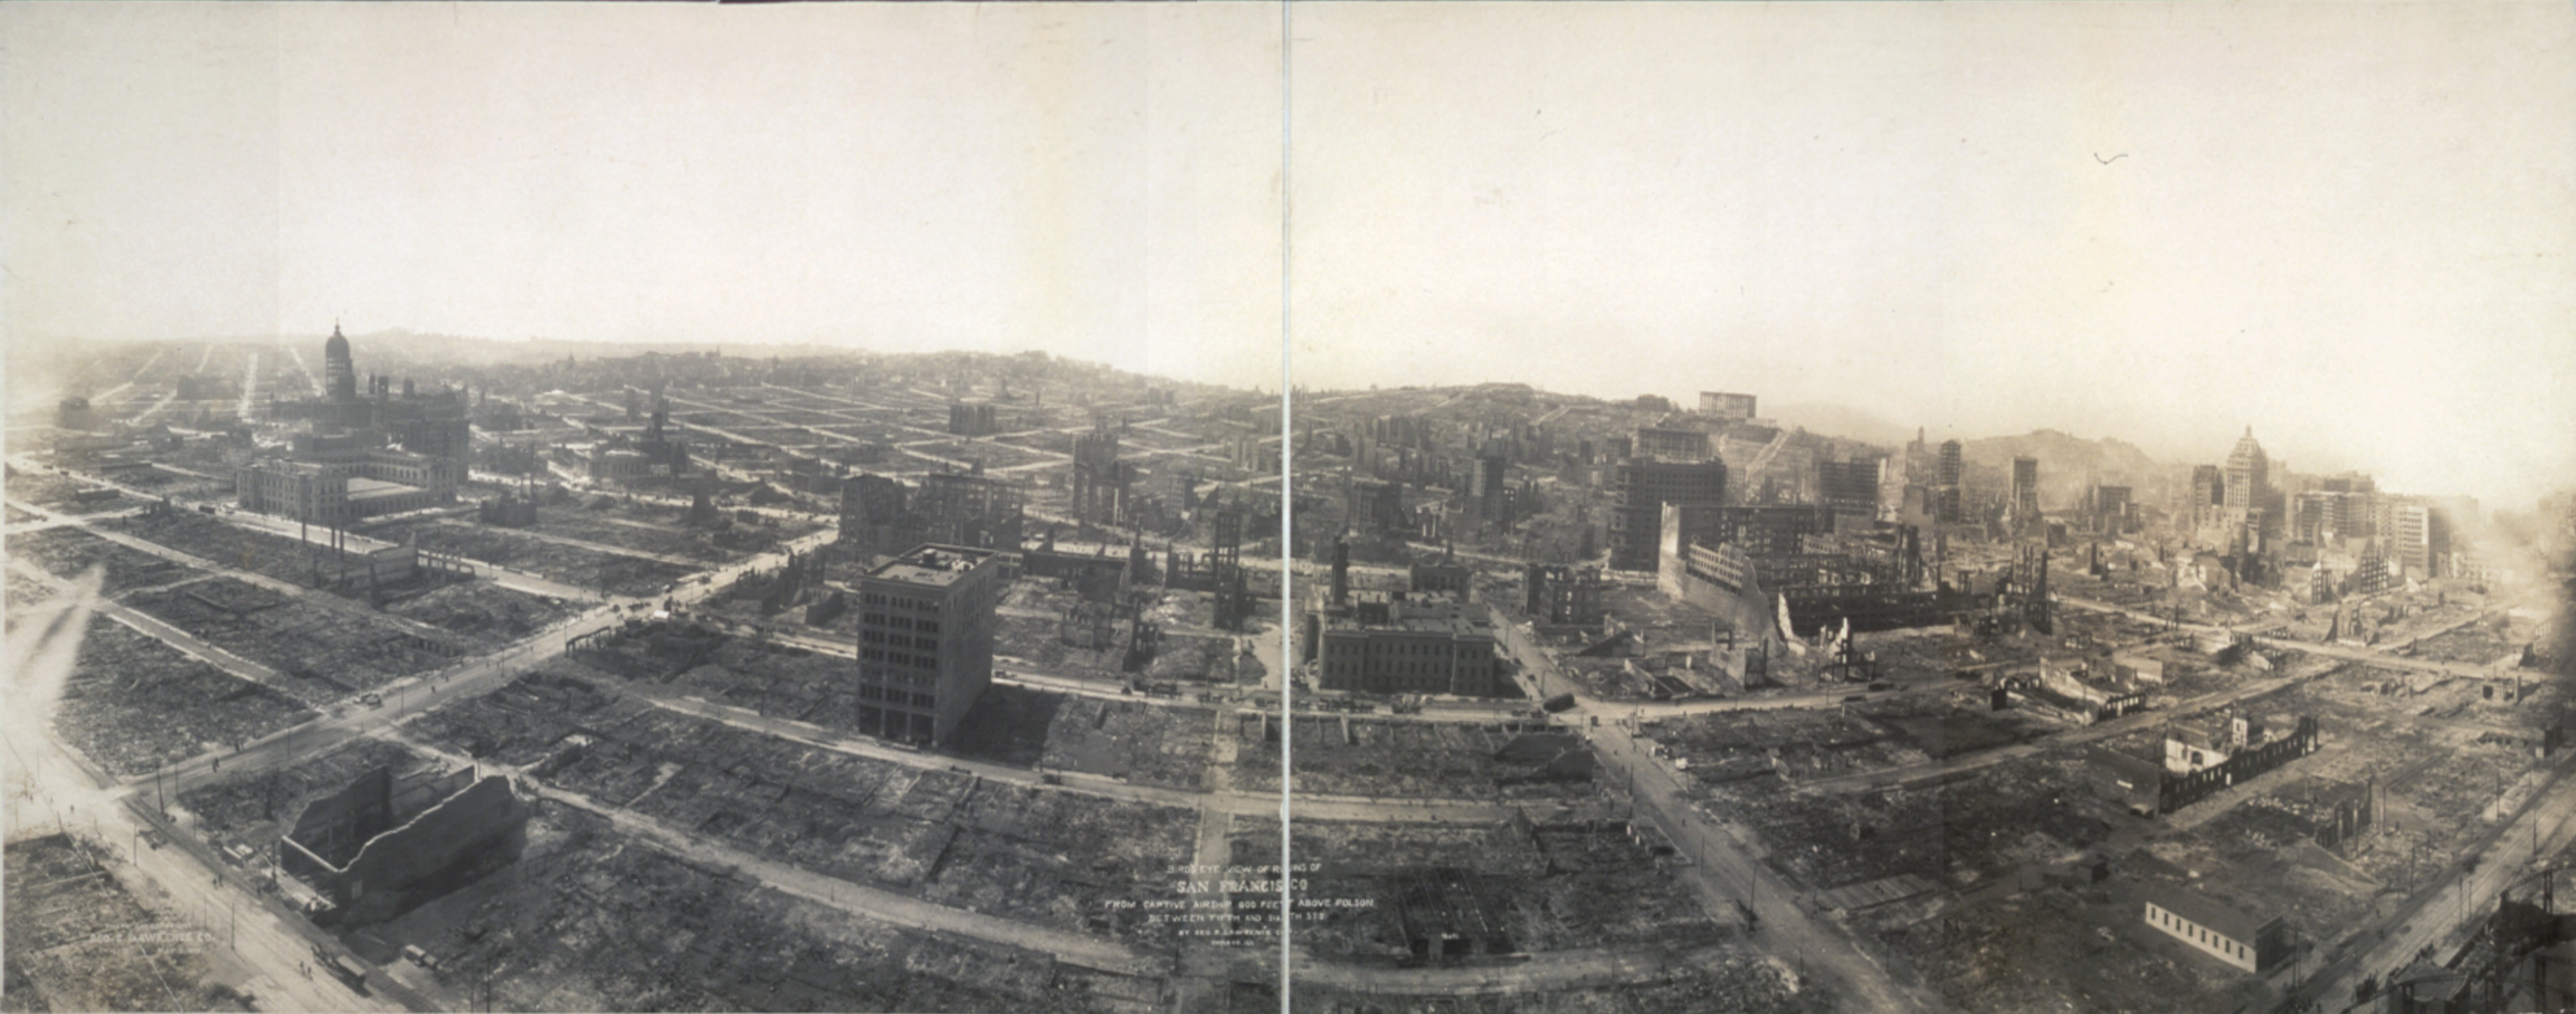
\includegraphics{figs/introduction/san_francisco_kitecamera.jpg}
	\caption{Photograph of San Francisco after the 1906 earthquake, taken from a camera held by seven kites. }
    \label{fig:san_francisco_kite}
\end{figure}

Satellite imaging, as known today, was first possible by the ideation of Konstantín Tsiolkovsky about rocketry to explore space, published under the title \textit{Exploring Space using jet propulsion devices}. This idea led to the first successful launch of the Sputnik satellite in 1957 and the development of Earth-orbiting satellites aimed at atmospherical monitoring. The Television and Infrared Observation Satellite (\acrshort{tiros}) was made operational in 1960 and integrated a small infrared system and a narrow-angle camera capturing data in the visible wavelengths. In 1978, a breakthrough change in satellites and coupled sensors came with \acrshort{tiros}-N (N for new). This spacecraft integrated a very high-resolution radiometer with 1 \si{\kilo\meter} footprint and four channels (visible, near-infrared, midrange-infrared and thermal infrared). Nowadays, an advanced version of these satellites is still operative under the name of \acrshort{avhrr} (Advanced Very High-Resolution Radiometer) with a similar footprint, though it captures six channels instead of four \cite{national_oceanic_and_atmospheric_administration_avhrr3_nodate}.   

\marginnote[.1cm]{An extensive repository of recent satellite missions can be found in the Earth Observation Portal, maintained by the European Space Agency \cite{earth_observation_portal_earth_nodate}.} 
From currently operative satellite programs, Landsat provides the largest collection of continuously acquired \acrshort{rs} data. It was first tested as part of NASA's NIMBUS program and there are currently two active satellites, Landsat-8 and Landsat-9, while the other seven have been terminated or planned to be decommissioned (Landsat-7). The payload of Landsat-9 consists of two instruments: Operational Land Imager (\acrshort{oli2}) and Thermal Infrared Sensor (\acrshort{tirs2}). A total of 11 bands and 740 scenes are collected every day, including red, blue, green, near-infrared, shortwave infrared, thermal, panchromatic, coastal and cirrus bands, ranging from a resolution of 15 \si{\meter} to 100 \si{\meter}. Other notable satellite programs are the China–Brazil Earth Resources Satellite (\acrshort{cbers}) and the Copernicus programme financed by the European Commission. The \acrshort{cbers}-4A satellite is equipped with three imaging tools capturing five different spectrum intervals with a spatial resolution of 2-55 \si{\meter} \cite{instituto_nacional_de_pesquisas_espaciais_inpecbers_2019}. On the other hand, the Sentinel-2 mission acquires 13 bands in the visible, shortwave and near-infrared spectrum (see Figure \ref{fig:sentinel2}) with a spatial resolution ranging from 10 \si{\meter} to 60 \si{\meter} \cite{european_environment_agency_eu_2017}. Its cycle to revisit the same Earth's location is ten days, in comparison with the 16 days needed by Landsat-9 or 31 days from \acrshort{cbers}-4A.

\begin{figure}[!ht]
	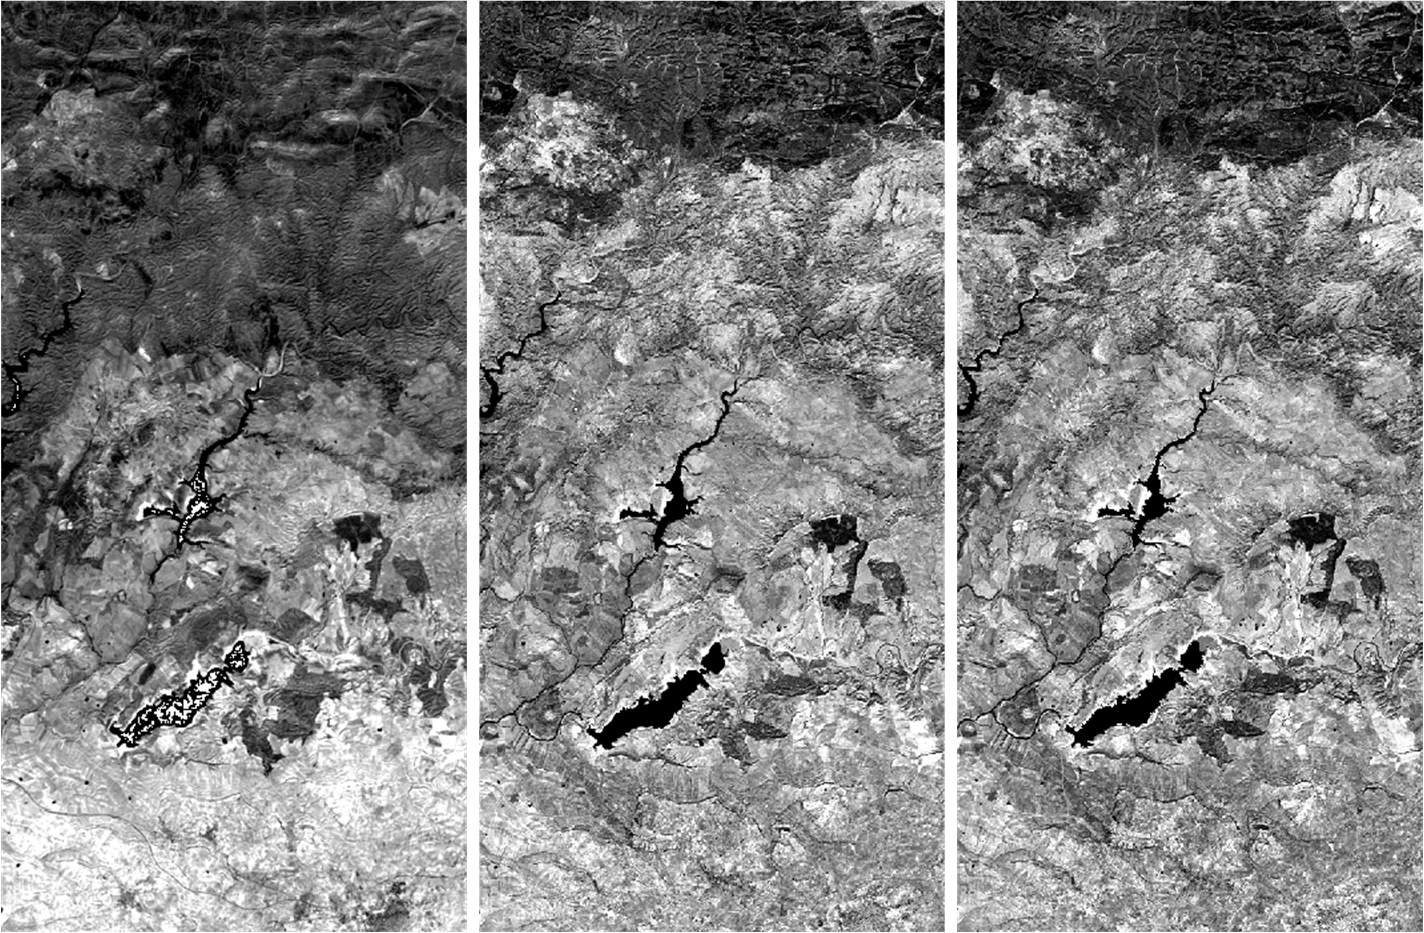
\includegraphics{figs/introduction/sentinel2_bands.png}
	\caption{Three shortwave infrared bands acquired by Sentinel-2 (band 9, 935-955 \si{\micro\meter}, band 11, 1567-1658 \si{\micro\meter}, and band 12, 2114-2889 \si{\micro\meter}). }
    \label{fig:sentinel2}
\end{figure}

As observed, the main limitations of satellite datasets are their temporal and spatial resolution. However, these drawbacks are being mitigated nowadays, especially by commercial missions. For instance, the commercial satellite Pléiades Neo (VHR-2020) from Airbus Defense \& Space \cite{airbus_pleiades_2021} is able to daily acquire seven bands with a Ground Sampling Distance (\acrshort{gsd}) of up to 30 \si{\centi\meter} for panchromatic images. Even for governmental missions, the repeat cycle is typically reduced as several twin missions could be active at the same moment with similar instruments and orbits. Accordingly, the offset in Landsat-8 and Landsat-9 trajectories allows acquiring data from the same point every 8 days \cite{masek_landsat_2020}. On the other hand, spatial resolution is steadily improving as most governmental restrictions have been lifted. Yet, spaceborne platforms are the most expensive Remote sensing technology by a huge lead. 

In addition to satellite imaging, the use of \acrshort{uas} has considerably increased over the last decade and has attracted the interest of both researchers and commercial applications. The most frequent components of remote sensing \acrshort{uas} are imaging sensors as well as navigation and communication systems. The latter allows the operator to manoeuvre the platform within a communication range and transfer data in a bidirectional stream. Regardless of the navigating mission, either manual or waypoint-based, Global Positioning System (\acrshort{gps}) and Inertial Measurement Unit (\acrshort{imu}) sensors are used to calculate and record the craft's position, orientation and movement. These components are especially relevant to perform accurate flight missions, and their precision is generally described by means of vertical and horizontal error in meters (\si{\meter}). In this regard, the most recent \acrshort{uas} series from DJI achieve vertical and horizontal errors of up to 10 \si{\centi\meter} using Real-time Kinematic (\acrshort{rtk}) positioning rather than \acrshort{gps}. As one would expect, \acrshort{uas} with lightweight and high-performance navigation sensors are more prohibitive.    

In terms of safety regulations, the term \acrshort{uas} does not only refer to the vehicle but also to the coupled sensors, which are following introduced. Sensors typically coupled on aircraft vary according to the platform's flight altitude and cruising speed as well as application requirements. Fixed and rotating wing \acrshort{uas} solutions are considerably more limited in flying height and speed than other airborne vehicles, including helicopters and gyroplanes. Apart from the platform limitations, the flight altitude may be limited by \acrshort{uas} regulations to avoid entering the domain of other airspace vehicles. Therefore, sensors and missions that require lower speed, lower flight altitude, and thus higher precision, are especially convenient for \acrshort{uas}. A widespread example of this is the monitoring of transmission lines, which happens to have a very thin structure and therefore require slower mapping. In comparison, other technologies such as Interferometric synthetic aperture radar (\acrshort{insar}) have been mainly applied to spaceborne missions to track changes on the Earth's surface.
\marginnote[-2.9cm]{The operability of unmanned aircraft over the Single European Sky airspace is controlled in the European Union by regulation 2019/947. Among other rules, the maximum flight altitude is established as 120 \si{\meter} over the Earth's surface unless an obstacle is overflown.} 

\section{Aims and objectives}

According to previously presented challenges, the overall aim of this dissertation is to contribute to some of the stages presented in Figure \ref{fig:introduction_scheme}. A significant number of challenges have already been briefly reviewed, including the collection of datasets from multiple sensors, difficulties in the correction and fusion of these, the generation of products with larger dimensionality (e.g., 2D $\rightarrow$ 3D) or the analysis of final products. Accordingly, the objectives of this work are the following:
\begin{itemize}
    \item The correction and processing of data as collected by airborne surveys. Rather than a single problem, this objective involves studying how can be every data source corrected, including geometrical and radiometric distortions. The first must be solved in most cases, since it enables the later fusion of data, whereas the latter depends on whether the radiance is further analyzed or not.
    \item The matching of images collected by different sensors, thus overcoming differences concerning 1) triggering timestamps, 2) optical aberrations, 3) optical systems and 4) wavelength intervals. The image matching ought to work over images with notable intensity dissimilarity to obtain reliable transformations that allow projecting one data source into another. 
    \item The efficient generation of large and dense 3D point clouds from multiple data sources without geometric inaccuracies. The proposed pipeline ought to tackle most of the drawbacks of traditional photogrammetry. In addition, this is a time-consuming task that is further stressed by including multiple data sources; hence, it must be addressed using accelerated computing.
    \marginnote[.0cm]{Despite visible, multispectral, thermal infrared and hyperspectral datasets covering a wide part of the spectrum, these will be projected to a 3D baseline point cloud generated with photogrammetry. Image-based reconstructions are less reliable than other optical sensing products, such as \acrshort{lidar}. However, it is also more cost prohibitive than most of the revised optical imaging sensors.}
    \item To emulate \acrshort{lidar} sensors over 3D synthetic scenarios. Nonetheless, this is also a time-consuming task that is especially tough to model in terms of returned intensity. The efficient generation of large labelled \acrshort{lidar} datasets must be addressed, again, using accelerating computing, by modelling the surfaces' properties.
    \item To demonstrate the applicability of previous results. Though not exhaustive, this objective involves detecting anomalies, segmenting some items apart from others or phenotyping a large number of vegetation varieties. It can be either performed with traditional geometry-based techniques as well as using \acrshort{ai} algorithms.
\end{itemize}

\section{Organization}

This dissertation comprises six different parts which are following detailed:

\newcommand{\partTabSize}{3mm}

\small \noindent \textbf{\textls[30]{PART I}} \normalsize\hspace{\partTabSize} This part includes the current chapter. A shallow introduction to \acrshort{rs} is presented together with the main challenges concerning data fusion. Then, the fundamentals of this dissertation are presented in Chapter \ref{sec:fundamentals_rs}, and later, a review of the state-of-the-art is given in Chapter \ref{sec:context_rs} to introduce previous work on the fusion and simulation of \acrshort{uas}-based data.

\small \noindent \textbf{\textls[30]{PART II}} \normalsize\hspace{\partTabSize} Here, the fundamentals of our methods are presented, including which kind of sensors and data are available. The correction and the image fusion algorithms are isolated in Chapter \ref{sec:image_fusion}. In summary, this part comprises the materials and methods that are shared among most of this dissertation's chapters.

\small \noindent \textbf{\textls[30]{PART III}} \normalsize\hspace{\partTabSize} This part explains the generation of 3D point clouds consisting of multiple layers: visible, infrared, multispectral and hyperspectral data. The visible colour is presented as the baseline 3D point cloud that is enhanced with the rest of the datasets. First, thermographic imagery is fused with \acrshort{rgb} data to propose an efficient projection in the Graphics Processing Unit, the so-called \acrshort{gpu}. This procedure is following applied to multispectral data, despite this being significantly more time-consuming and intricate since the latter comprises four spectral bands. Then, a hyperspectral point cloud is generated following a different pipeline, yet accelerated, that fits the conditions on which these data were acquired.  

\small \noindent \textbf{\textls[30]{PART IV}} \normalsize\hspace{\partTabSize} Instead of correcting and fusing real-world datasets, others are simulated using detailed synthetic scenarios that are rapidly labelled with semantic tags. Simulations are aimed at modelling products similar to those collected by real sensors, including their geometrical properties. The fundamentals of \acrshort{lidar} simulations are reviewed in Chapter \ref{sec:lidar_simulation}, whereas radiance properties require further considerations which are detailed in Chapter \ref{sec:lidar_intensity}. Then, these simulations are used to assist in the scanning of indoor scenarios such as buildings in Chapter \ref{sec:lidar_optimization}.

\small \noindent \textbf{\textls[30]{PART V}} \normalsize\hspace{\partTabSize} This part shows multiple applications of the collected data and the derived results, including the simulated \acrshort{lidar} point clouds, reconstructed thermal point clouds and hyperspectral swaths. The first are Thermal infrared data are applied to the detection of thermal anomalies that may be linked to buried remains at an archaeological site. Hyperspectral swaths are, on the other hand, corrected and processed for the classification of red and white grapevine varieties using Deep Learning.

\small \noindent \textbf{\textls[30]{PART VI}} \normalsize\hspace{\partTabSize} Chapter \ref{sec:conclusions} concludes this dissertation by highlighting the main contributions and pointing out future work.
\setchapterpreamble[u]{\margintoc}
\chapter{Fundamentals of imaging sensors}
\labch{fundamentals}
\label{sec:fundamentals_rs}

% \addtocounter{page}{-1}

The main goal of imaging sensors is to obtain measurements from objects and processes to extract quantitative, visual and text-based results. The most frequent form of \acrshort{rs} results are images, and the science and technology that transforms images into valuable products is known as photogrammetry. Images are derived from passive sensors that capture the incoming radiance from the surrounding environment. The technology involved in this will be briefly discussed in Section \ref{sec:fundamentals_optical_imaging_geometry}. However, other kinds of sensors operate as active technologies that emit and receive backscattered light from the Earth's surfaces. The latter technology directly captures the geometry of the impacted surfaces, though images can also be derived from these products. The use of active and passive sensors depends on the budget, the required products and how will the conclusions be extracted from these products. In this regard, passive imaging sensors are typically cheaper and 3D reconstructions derived from these may lack accuracy despite being supported by reference data. On the other hand, the results from active sensors record the geometry of items instead of reconstructing them and they are also less likely to be altered by atmospheric effects. As opposed to passive results, deriving imagery from geometry may have some disadvantages due to non-uniform densities and lack of spatial resolution over the covered area. Hence, both technologies have their downsides and thus must be used as complementary data sources.

This section is structured as follows. First, optical imaging systems are presented to cover visible, thermographic and multispectral sensing tools. Then, the fundamentals of \acrshort{lidar} technology are introduced as another optical imaging technique. Finally, some of the most frequent operations performed over the data collected by the revised sensors are then presented to introduce the reader to the basics. 

%Finally, the state-of-the-art concerning the fusion of results from previously described technologies is presented, together with the synthetic generation of sensing information. The understanding of \acrshort{lidar} sensors is especially relevant for the latter context, as previous work simulates the functioning of active optical systems. 

\section{Optical imaging systems} 

The underlying concept in \acrshort{rs} is to measure the emitted energy from the Earth's surfaces either from excitation of internal processes or interaction with incoming energy. We refer to energy as electromagnetic (\acrshort{em}) radiation that travels through time and space with a wave-like shape. If these are unpolarized, they oscillate in all the directions that are perpendicular to the travelling vector. The number of oscillations is known as frequency ($\nu$), whereas the spacing between two successive crests is the wavelength, $\lambda$. In a vacuum, \acrshort{em} radiation travels at the speed of light, $c = \lambda * \nu$; in nature, it depends on the traversed medium. The fundamental unit in \acrshort{em} radiation is the photon, the physical form of a quantum, and these units are the target of the following described optical imaging tools \cite{emery_introduction_2017}. These are designed to capture \acrshort{em} radiation passing through a polarized filter, thus focusing on a specific spectral interval.

The early cameras were simply light-tight boxes with a pinhole from where the light was allowed to pass through. The exposure of the film was controlled by letting light pass or not through it. Then, they were replaced by lenses aimed at enlarging the hole, thus capturing more light in less time. Besides lenses, these systems were also composed of a diaphragm adjusting the diameter of the lens opening, and a shutter that controlled the exposure time. Nowadays cameras are not that different from these early cameras, though they have now better control over the focus and exposure. The main concern of this dissertation are sensors measuring \acrshort{em} radiation as functions of location ($x, y$), time and wavelength ($\lambda$). These sensors are classified into imagers, which produce two and three-dimensional images, and nonimagers, such as hand-held devices that output single response values. 

Imagers are also known as radiometers, and these instruments require decomposing the radiation contributions and quantifying them with matched detectors. The first dispersion method is a prism, which was first utilized to separate out wavelengths by Isaac Newton. This dispersion results from refractivity being dependent on wavelength, causing entering light rays to exit at different angles. Other dispersion mechanisms are filter-wheel radiometers, grating spectrometers and interferometers, where the former is the most widespread. Filter-wheel radiometers separate wavelengths using a wheel, composed of radiative filters, that cycles through the radiation path. Filters can be classified as absorption- or interference-based, though only the first is integrated into a filter-wheel. They can be designed to let through long, short or very narrow wavelength bands, defined by a central wavelength and cutoff limits. Coloured absorption filters are made of coloured glass or dyed gelatin that absorbs energy from a wavelength interval and let others pass. Furthermore, filters also attenuate the passing radiation, and their radiative efficiency is given by the signal-to-noise ratio (\acrshort{snr}).

On the other hand, the transmitted energy must be captured into images. The transition from analogical to digital photography was led by utilizing solid-state sensors instead of silver halide crystals, with the first being more sensitive to brightness changes. Digital cameras incorporate two-dimensional arrays of semiconductors, either charge-coupled devices (\acrshort{ccd}) or complementary metal-oxide (\acrshort{cmos}). Each one of these detectors is dedicated to sensing the energy for an image's pixel. The scene brightness captured in that pixel is proportional to the small electrical charge triggered by the striking energy. Charges are transformed to voltage values using the photodetector's area and responsivity, the incoming radiance and the spectral width, followed by analogical to digital (A-to-D) conversion. Although semiconductors are monochromatic, \acrshort{rgb}-colour data can be obtained by placing filters over these photosites in the sensor array with a Bayer pattern. Red, green and blue photosites are arranged so that missing colour data can be interpolated from surrounding photosites with the same colour. With this pattern, half the filters are green, while the remainder is equally split into blue and red. Other detectors are able to record red, green and blue radiance at every pixel, such as Foveon \acrshort{cmos} \cite{lillesand_remote_2015}. Besides \acrshort{rgb}, hyperspectral imaging constitutes a greater challenge as it does not require capturing three simultaneous wavelengths, but hundreds of narrow bands. Hence, photo-detectors are arranged as arrays along the spatial and spectral dimensions. Depending on the wavelength range, the material in which semiconductors are made varies; from silicon (visible) to PbS (lead sulfide, near-IR) or InSb (indium-antimony, mid-IR). 

The overall objective of imaging spectrometers is to observe large portions of the Earth and therefore, to progressively build data cubes recording spectral and spatial information. However, it is possible to scan the area of interest with hundreds and thousands of images or simply with a few of them that are built as the scanning platform translates, thus yielding larger images than usual. 

\subsection{Scan geometry}
\label{sec:fundamentals_optical_imaging_geometry}

At least three scanning geometries are distinguished, involving different mechanical and optical principles: single-snapshot, whiskbroom and push broom. Further insight into push broom and snapshot scanning is provided in Figure \ref{fig:hyper_scan_geometry}. 

\begin{figure*}[!ht]
	\includegraphics[width=\linewidth]{figs/context/hyper_sources.png}
	\caption{Mechanism involved in a) push broom and b) single-snapshot scanning geometries.}
    \label{fig:hyper_scan_geometry}
\end{figure*}

Single-snapshot is the most widespread scanning geometry. Matrices of semiconductors simultaneously acquire spatial and spectral information from the area of interest. Therefore, there is no scanning involved; it captures a single snapshot with limited spatial resolution. The main drawbacks are given by the dimensionality of \acrshort{ccd} arrays, as they bound the number of pixels. Although it is possible to increase spatial or spectral resolution by enlarging \acrshort{ccd} arrays, it may come at the expense of reducing the dimensionality of one axis. This is especially relevant for imaging devices producing large data cubes, e.g., hyperspectral. Despite the advent of large detectors measuring millions of voxels at the same time, the already huge size of hyperspectral \acrshort{ccd}s forbids enlarging axes without penalizing others \cite{sousa_uav-based_2022, pu_hyperspectral_2017}. 

On the other hand, push-broom or line-scanning is possible with a 2D matrix of semiconductors ($\lambda \times x$) recording data in the spectral, $\lambda$, and spatial, $x$, dimensions. Since the \acrshort{ccd} array is 2D, horizontal sweeps are acquired simultaneously (lines), and these are accumulated into images known as swaths. Thus, this approach requires a mobile platform or imaging device that moves forward and helps to enlarge the observed area in $y$. Rather than a complex mechanical system, this scanning requires an optical design that collects radiation with pointing mirrors and collimates it into dispersing elements \cite{sousa_uav-based_2022, pu_hyperspectral_2017}. 

Whiskbroom geometry is halfway into single-snapshot and push-broom. The core of this approach is a rotating mirror that dispersers radiation through a grating plane or prism into a linear \acrshort{ccd} array with a dimensionality of $\lambda$. Hence, it requires a lesser number of photo-detectors than previous scanning geometries and consequently, these devices are easier to calibrate while providing a high spectral resolution and radiative sensitivity. Due to the acquisition mechanism, the dwell time on every pixel is also smaller, which leads to a lower Signal-to-Noise Ratio (\acrshort{snr}). However, the misalignment of bands in single-snapshot and lines in push-broom is here found at the pixel level, thus hardening the generation of orthorectified products \cite{pu_hyperspectral_2017}.

Besides the scanning geometry, aerial photographs are taken along flight lines and thus their acquisition setup also matters for the final results. First, these are recorded along a viewing direction, with $\textit{nadir}$ being the most trivial, i.e., perpendicular to the soil represented as a horizontal plane. Furthermore, successive images are taken with a degree of overlapping, either frontal or side overlap. It guarantees that features are visible in more than one image, thus leading to stereoscopic pairs and stereoscopic coverage. Frontal overlap refers to the overlapping between successive images in the same flight strip, whereas side overlap is the degree of overlapping among consecutive strips. The geometric elements of a vertical photograph are straightforward, considering that $o$ is the principal point, i.e., the intersection of the optical axis with the film plane, whereas the optical axis controls the view direction. In Figure \ref{fig:nadir_image_scan}, the photograph is taken with \textit{nadir} view direction.
\begin{marginfigure}[-5cm]
    \centering
    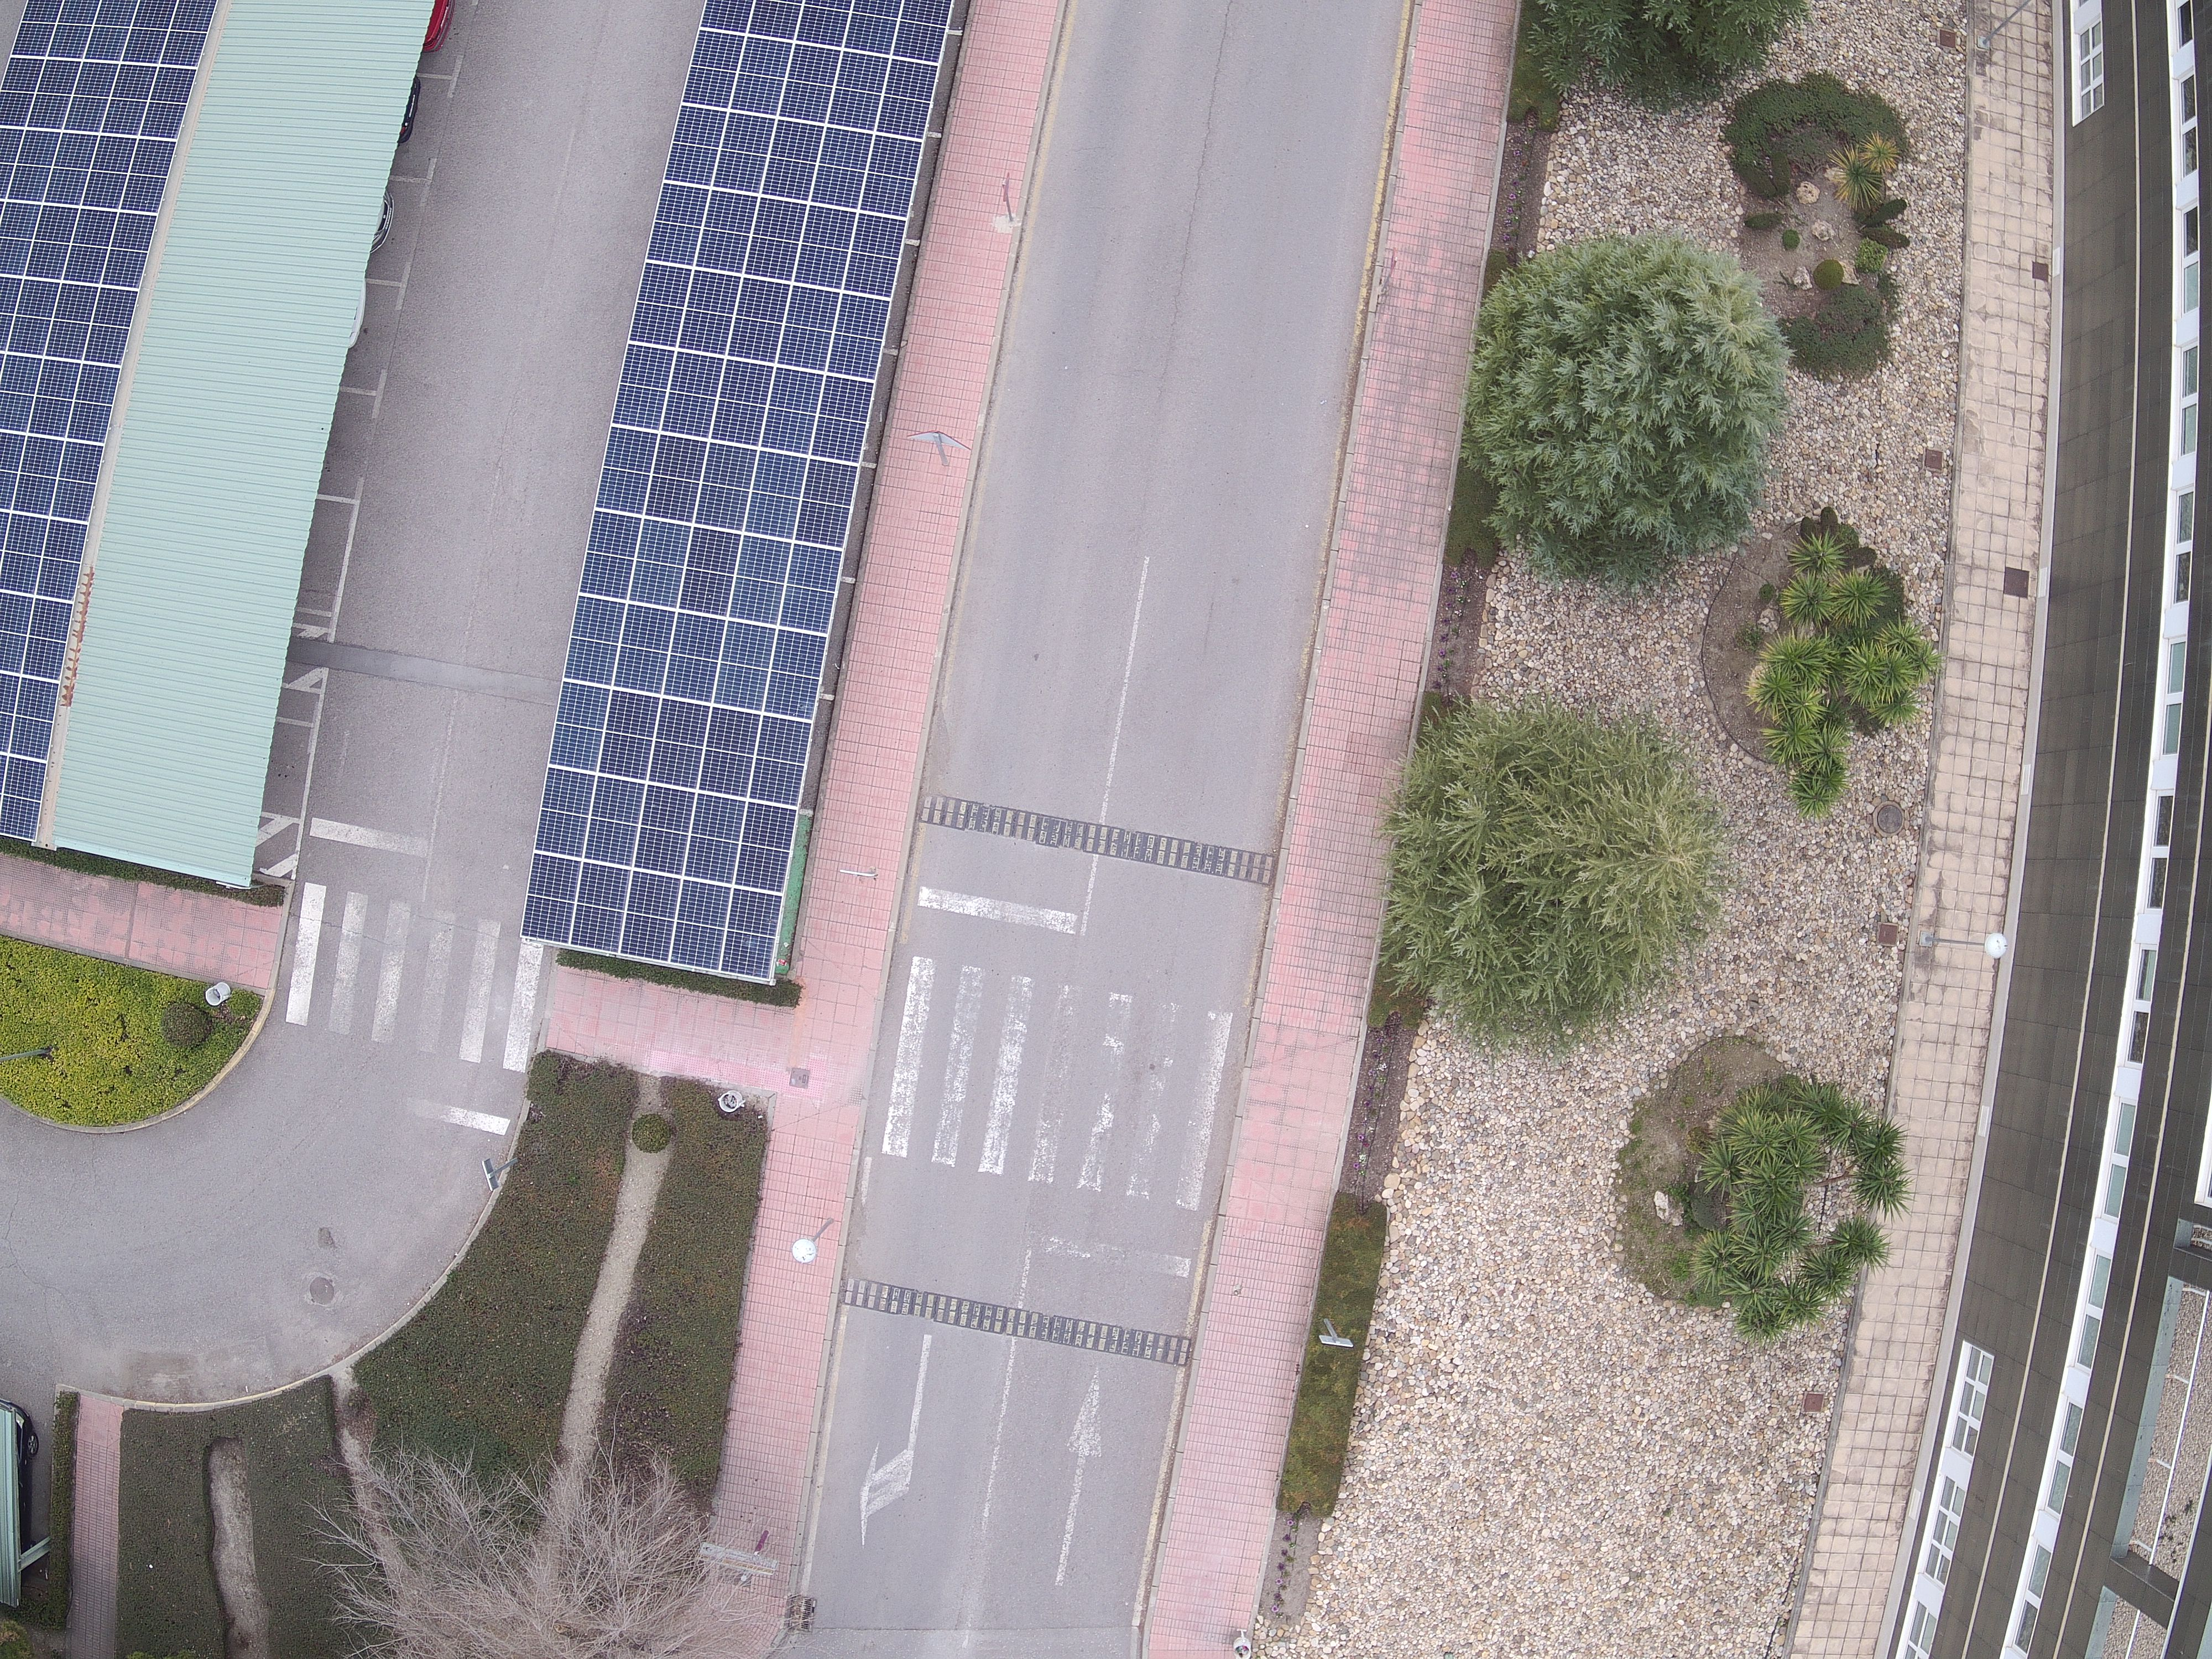
\includegraphics{figs/fundamentals/nadir_image_scan.jpg}
    \caption{Image captured during a flight planned with \textit{nadir} view direction.}
    \label{fig:nadir_image_scan}
\end{marginfigure}

The following sections present the most widespread imaging sensing tools and those that will be covered in the methodology of this work.

\subsection{Multispectral imaging}
\label{sec:multispectral_imaging}

Multispectral images consist of multiple bands corresponding to different wavelengths. However, these are typically discrete readings of spectral intervals with varying bandwidths. Most of the research and academic work describe multispectral as a special case of super spectral and hyperspectral imagery, and so we will, though some remarks are mentioned in this section for our later work. First, Table \ref{table:multispectral_devices} presents some of the multispectral sensors that are frequently revised in the literature, along with the works where they were mentioned. The discrete wavelengths and the resolution of every reading are shown in the fifth column, \textit{Spectral bands}. It can be observed that only a few bands with a coarse resolution, ranging from 14 \si{\micro\meter} to 57 \si{\micro\meter}, are recorded.

\renewcommand{\arraystretch}{1.2}
\begin{table*}[htb]
    \caption{Consumer-grade multispectral devices found in the literature and their specifications, according to the manufacturer's source.}
    \label{table:multispectral_devices}
    \begin{tabular}{llllll}
        \toprule
        Multispectral tool & Focal length & HFOV & Image resolution & Spectral bands (\si{\micro\meter}) & Ref. work \\
        \midrule
        \multicolumn{6}{c}{Parrot}\\
        \cmidrule{1-6}
        \multirow{4}{*}{Sequoia}     & \multirow{4}{*}{3.98 \si{\milli\meter}}   & \multirow{4}{*}{$63.9^{\circ}$}  & \multirow{4}{*}{$1280 \times 960$ px}  & Green: $5.5 \pm 0.2$  & \multirow{4}{*}{\cite{franzini_geometric_2019}}\\
        & & & & Red: $6.6 \pm 0.2$ &\\
        & & & & Red-Edge: $7.35 \pm 0.05$ &\\
        & & & & Near-IR: $7.9 \pm 0.2$ &\\
        \cmidrule{1-6}
        \multicolumn{6}{c}{Micasense}\\
        \cmidrule{1-6}
        \multirow{5}{*}{RedEdge-MX}     & \multirow{5}{*}{5.4 \si{\milli\meter}}   & \multirow{5}{*}{$47.2^{\circ}$}  & \multirow{5}{*}{$1280 \times 960$ px}  & Blue: $4.75 \pm 0.16$     & \multirow{5}{*}{\cite{cunha_prediction_2021, isgro_unmanned_2021}}\\
        & & & & Green: $5.6 \pm 0.13$ &\\
        & & & & Red: $6.68 \pm 0.07$ &\\
        & & & & Red-Edge: $7.17 \pm 0.06$ &\\
        & & & & Near-IR: $8.42 \pm 0.28$ &\\
        \cmidrule{1-6}
        \multirow{10}{*}{Dual-Camera}     & \multirow{10}{*}{5.4 \si{\milli\meter}}   & \multirow{10}{*}{$47.2^{\circ}$}  & \multirow{10}{*}{$1280 \times 960$ px} & Coast blue: $4.44 \pm 0.14$    & \multirow{10}{*}{\cite{chakhvashvili_comparison_2021}}\\
        & & & & Blue: $4.75 \pm 0.16$ &\\
        & & & & Green 1: $5.31 \pm 0.07$ &\\
        & & & & Green 2: $5.6 \pm 0.13$ &\\
        & & & & Red 1: $6.5 \pm 0.08$ &\\
        & & & & Red 2: $6.68 \pm 0.07$ &\\
        & & & & Red-Edge 1: $7.05 \pm 0.05$ &\\
        & & & & Red-Edge 2: $7.17 \pm 0.06$ &\\
        & & & & Red-Edge 3: $7.4 \pm 0.09$ &\\
        & & & & Near-IR: $8.42 \pm 0.28$ &\\
        \cmidrule{1-6}
        \multirow{6}{*}{Altum}     & \multirow{5}{*}{8 \si{\milli\meter}}   & \multirow{5}{*}{$50^{\circ}$}  & \multirow{5}{*}{$2064 \times 1544$ px} & Blue: $5.75 \pm 0.16$    & \multirow{6}{*}{\cite{hutton_high_2020}}\\
        & & & & Green: $5.6 \pm 0.13$ &\\
        & & & & Red: $6.68 \pm 0.07$ &\\
        & & & & Red-Edge: $7.17 \pm 0.06$ &\\
        & & & & Near-IR: $8.42 \pm 0.28$ &\\
        \cmidrule{2-6}
        & \multirow{1}{*}{1.77 \si{\milli\meter}} & \multirow{1}{*}{$57^{\circ}$} & \multirow{1}{*}{$160 \times 120$ px} & Long-Wave IR: $11 \pm 3$ &\\
        \cmidrule{1-6}
        \multirow{6}{*}{Altum-PT}     & \multirow{5}{*}{8 \si{\milli\meter}}   & \multirow{5}{*}{$50^{\circ}$}  & \multirow{5}{*}{$2064 \times 1544$ px} & Blue: $5.75 \pm 0.16$    & \multirow{6}{*}{\cite{hutton_high_2020}}\\
        & & & & Green: $5.6 \pm 0.13$ &\\
        & & & & Red: $6.68 \pm 0.07$ &\\
        & & & & Red-Edge: $7.17 \pm 0.06$ &\\
        & & & & Near-IR: $8.42 \pm 0.28$ &\\
        \cmidrule{2-6}
        & \multirow{1}{*}{1.77 \si{\milli\meter}} & \multirow{1}{*}{$48^{\circ}$} & \multirow{1}{*}{$320 \times 256$ px} & Long-Wave IR: $10.5 \pm 3$ &\\
        \cmidrule{1-6}
        \multicolumn{6}{c}{DJI}\\
        \cmidrule{1-6}
        \multirow{5}{*}{P4 Multispectral}     & \multirow{5}{*}{5.74 \si{\milli\meter}}   & \multirow{5}{*}{$62.7^{\circ}$}  & \multirow{5}{*}{$1600 \times 1300$ px} & Blue: $4.5 \pm 0.08$    & \multirow{5}{*}{\cite{lu_experimental_2020}}\\
        & & & & Green: $5.6 \pm 0.08$ &\\
        & & & & Red: $6.5 \pm 0.08$ &\\
        & & & & Red-Edge: $7.3 \pm 0.08$ &\\
        & & & & Near-IR: $8.4 \pm 0.08$ &\\
        \bottomrule
    \end{tabular}
\end{table*}
\renewcommand{\arraystretch}{1}

\marginnote[3cm]{For tasks such as vegetation classification, visible and near-infrared bands from multispectral imagery are sufficient in most cases. Bare soils tend to show a more constant spectral signature, whereas vegetation presents a steeper slope with higher values in the near-infrared wavelengths \cite{navulur_multispectral_2006}.}
The most frequently recorded bands are Red, Green, Blue, Red-Edge (\acrshort{reg}) and Near-Infrared (\acrshort{nir}), thus overlapping with previous and later imaging tools (visible and thermographic cameras). \acrshort{reg} bands are halfway between Red and \acrshort{nir}, while \acrshort{nir} overlaps with Long-wave Infrared (\acrshort{lwir}) wavelengths. Despite other sensors being able to capture most of these individual bands, multispectral imaging opens a wide number of opportunities by simultaneously recording bands sparsed throughout the visible and infrared spectrum. Most of the multispectral applications benefit from multiple bands through the so-called indices, i.e, linear combinations of them aimed at highlighting relevant features in a group of target objects. In this regard, a total of 82 spectral vegetation indices were collected from the literature by Pu, Ruiliang \cite{pu_hyperspectral_2017}. A recurrent vegetation index in \acrshort{pa} work is the \acrshort{ndvi} (Normalized difference vegetation index), calculated as a combination of Red and \acrshort{nir} bands. Besides identifying vegetation, other indices are focused on estimating pigments and chlorophyll content in plants \cite{pu_hyperspectral_2017}. Most of them work by aggregating bands where the target compound has the most and less significant presence, while others are rather aimed at simply detecting its presence.

\begin{marginfigure}[1.5cm]
    \centering
    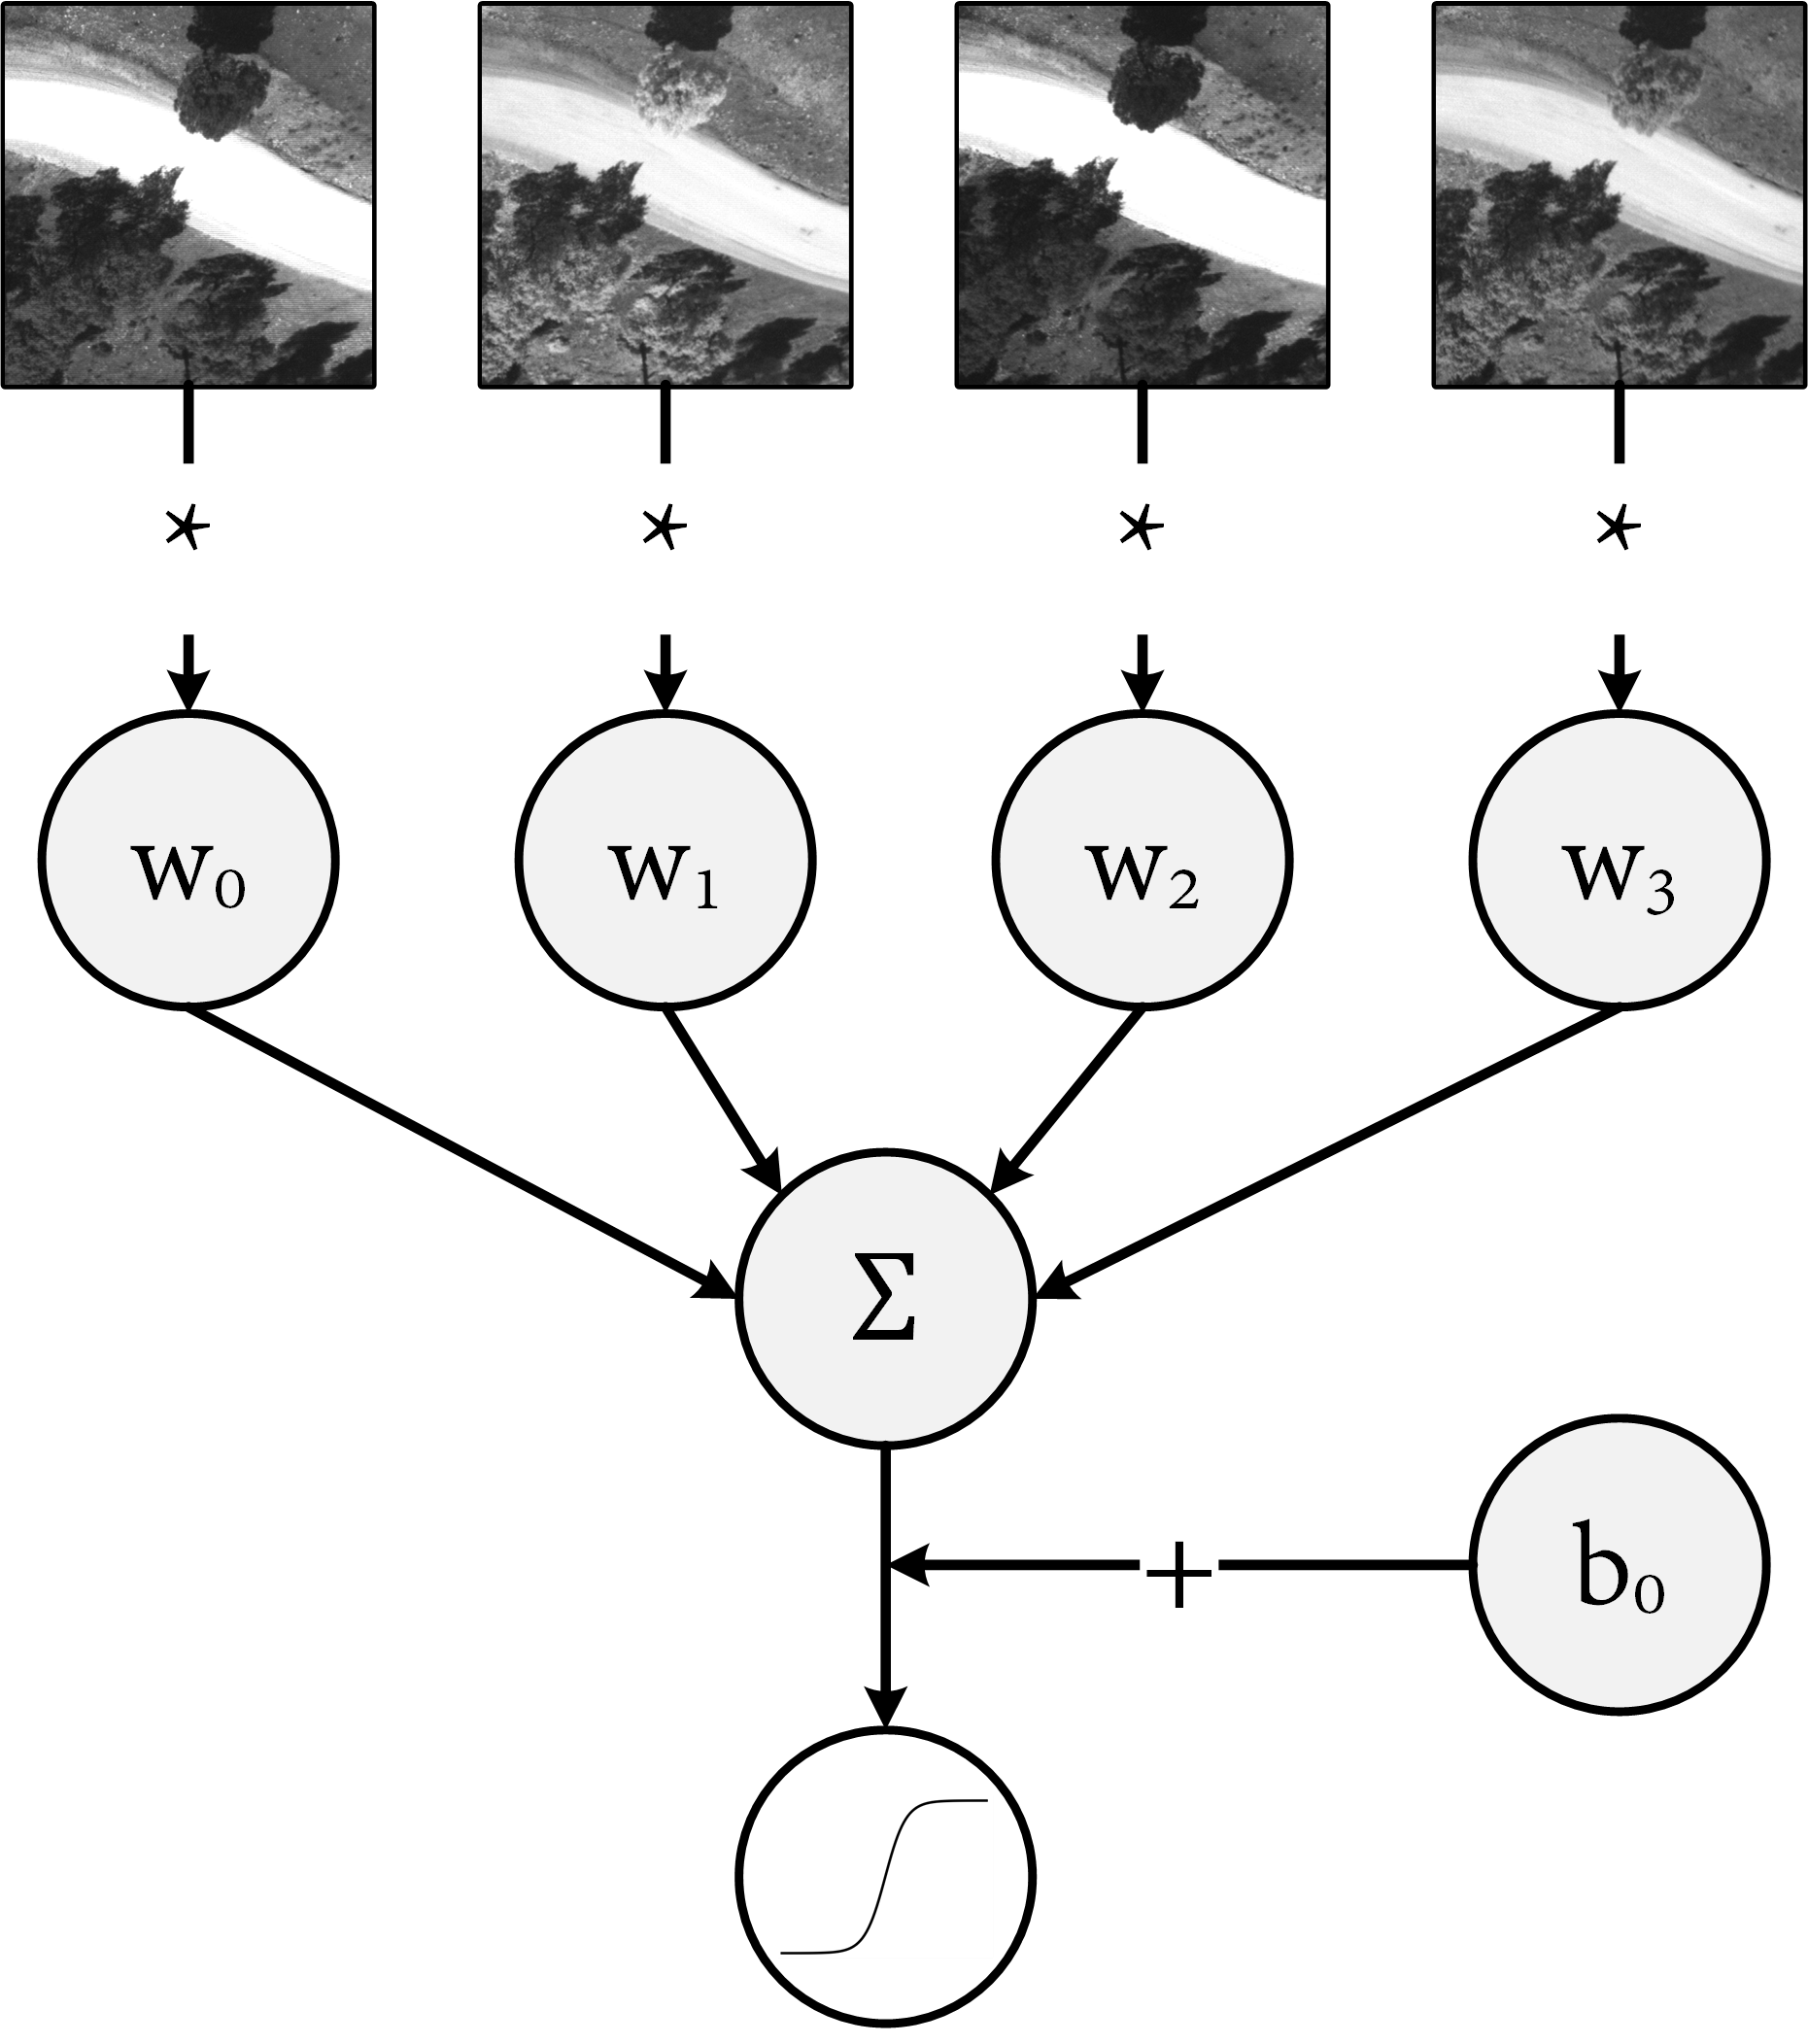
\includegraphics{figs/fundamentals/cnn_ndvi.png}
    \caption{Architecture of a simple neural network with a single layer, aimed at learning the weights of importance of every spectral band.}
    \label{fig:cnn_dvi}
\end{marginfigure}
\begin{kaobox}[frametitle=Activation of relevant spectral bands]
As explained, the aim of spectral indices is to measure or simply indicate the presence of a compound: vegetation, water, etc. A rapid way to determine which bands have a higher weight to highlight a certain compound is to train a trivial neural network with five trainable parameters (Figure \ref{fig:cnn_dvi}). These correspond to four weights ($W^{4\times1}$) belonging to Green, \acrshort{nir}, Red and \acrshort{reg} spectral bands, plus one bias, $b^{1}$. It can be trained over perfectly overlapped multispectral datasets, where the ground truth annotates vegetation and ground. Neither it is a great classifier nor do we plan it to be as so. It was randomly initialized, and the first fitting obtained an overall accuracy close to 98\% and yielded $W = \left[-3.6329935, 33.97777, -67.50758, 2.1926873\right]^{\intercal}$. Hence, \acrshort{nir} and Red bands had a higher contribution to the computed probability, which also happens to correspond to $w_2 \cdot \textit{\acrshort{nir}}$ - $w_3 \cdot \textit{Red}$. \acrshort{ndvi} is, on the other hand, defined in Equation \ref{eq:ndvi}:
\begin{equation}
    \textit{NDVI} = \frac{\textit{NIR} - \textit{Red}}{\textit{NIR} + \textit{Red}}
    \label{eq:ndvi}
\end{equation}
where the aim of $\textit{\acrshort{nir}} + \textit{Red}$ is to normalize the contribution of both spectral bands so that it is minimized when $\lim_{\textit{\acrshort{nir}} \to \textit{Red}} \textit{\acrshort{ndvi}} = 0$ and maximized if $\lim_{\textit{\acrshort{nir}} \to 1 - \textit{Red}} \textit{\acrshort{ndvi}} = 1$, with \acrshort{nir}, Red $\in [0, 1]$. Therefore, the numerator was directly explained by a neural network with a single dense layer, whereas the normalization can be achieved with a simple sigmoid activation, $x \gets w_2 \cdot \textit{\acrshort{nir}}$ - $w_3 \cdot \textit{Red}; s(x) =  \frac{1}{1 + e^{-x}}$, to output a probability $s(x) \in [0, 1]$. It is intended to approximately infer and emulate the $\textit{\acrshort{ndvi}}$ formula; nevertheless, neither $s(x)$ is linear as defined nor the weights were accurately estimated (note that $w_3 > -2 \cdot w_2$).  
\end{kaobox}

However, the revision of vegetation indices converges into the previously mentioned shortcomings of multispectral imagery. Most of these indices operate very specific wavelengths, e.g., 670, 800, 1050, etc., while only a few bands are captured in multispectral imaging. Although it is possible to approximate missing wavelengths with the most similar bands, as shown in Code \ref{code:nearestband}, the results are far from optimal. Therefore, multispectral imaging is better suited for trivial applications such as vegetation classification, while it is not sufficient for other applications that require lower spectral resolution, such as mineral mapping or classifying vegetation species \cite{navulur_multispectral_2006, pu_hyperspectral_2017}. Indeed, most of the metrics proposed in the literature for discerning spectral signatures are based on their derivative. On the other hand, multispectral bands represent a step function with some intervals being undefined.

\lstinputlisting[language=python, caption={Function for finding the most similar wavelength among those available for a specific sensor data.}, label=code:nearestband]{code/nearest_band.py}

Recently, novel aerial platforms and multispectral sensors are emerging in order to increase the accuracy of spectral measurements, reduce the noise coming from different layers of the atmosphere, and increase the model coverage by multiple view-points with a higher spatial resolution \cite{deng_uav-based_2018}. The \acrshort{uas}’s capabilities to carry lightweight imaging systems have positively impacted recent research. In contrast to satellite images, the \acrshort{gsd} of \acrshort{uas}-multispectral imagery can be significantly reduced to a few centimetres. The increase in spatial resolution and the possibility to capture many overlapped images enable the development of image-based techniques for 3D model reconstruction.

Finally, remark that the processing of multispectral imagery from commercial devices is performed with proprietary software and formulae defined by manufacturers. The acquired irradiance at discrete wavelengths is not transformed in a manner that involves the spectral signature. Instead, irradiance is typically turned into reflectance using the shutter speed, the observation angle, the gain factor and other calibration coefficients, either provided by the manufacturer or obtained before and after flights \cite{jurado_semantic_2020, candiago_evaluating_2015}.

\subsection{Thermography}
\label{sec:thermography_imaging}

\begin{marginfigure}[1.5cm]
    \centering
    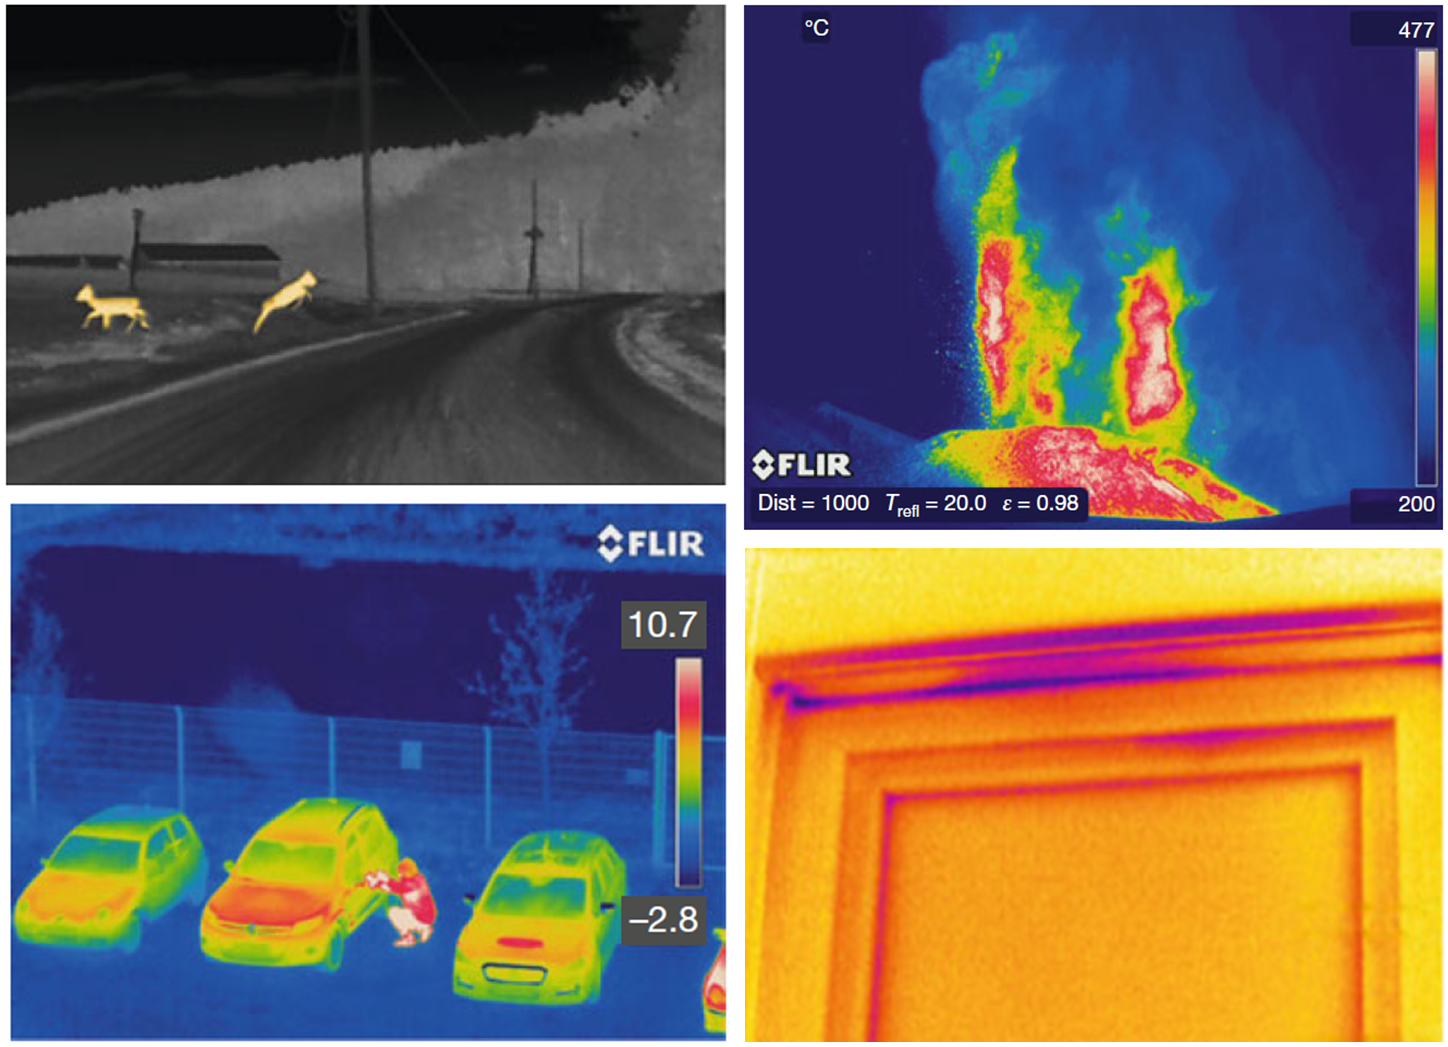
\includegraphics{figs/fundamentals/thermal_applications.png}
    \caption{Some applications of infrared imaging \cite{vollmer_infrared_2017}. From left to right, and from top to bottom: night vision, volcano monitoring, surveillance and detection of incorrect thermal insulation.}
    \label{fig:thermal_applications}
\end{marginfigure}
Infrared thermal imaging (\acrshort{ir}) or thermography is a noninvasive technology for acquiring the temperature of objects' surfaces and phenomena through their emitted radiation. In recent years, rapid growth has been witnessed due to the progress made in the technology of infrared detectors. Furthermore, the competition among camera manufacturers has led to releasing low-cost \acrshort{ir} products, thus widening the applicability scope and diversity of customers. It is considered an excellent noninvasive technology, and therefore, it is applied over very different scopes. Some of the most revised applications in the literature are quality control and monitoring in industrial environments \cite{alfredo_osornio-rios_recent_2019, vollmer_infrared_2017}, medical analysis \cite{lorinczy_thermal_2017}, building inspection \cite{jarzabek-rychard_supervised_2020, kylili_infrared_2014}, agriculture and animal applications \cite{mcmanus_infrared_2016, tsouros_review_2019}, geological monitoring \cite{grechi_3d_2021}, fire and gas leaks detection \cite{gade_thermal_2014}, surveillance, etc. (see Figure \ref{fig:thermal_applications}). On crop and forest management, it has been mainly applied to tree characterization by measuring their energy flux, evapotranspiration and photosynthesis \cite{webster_three-dimensional_2018}, as well as for water stress and disease detection \cite{yandun_narvaez_survey_2017, de_oca_uas_2021, zarco-tejada_previsual_2018}. Heating monitoring also prevents frost damage from crops \cite{yuan_uav-based_2021}. 

\begin{marginfigure}[.15cm]
	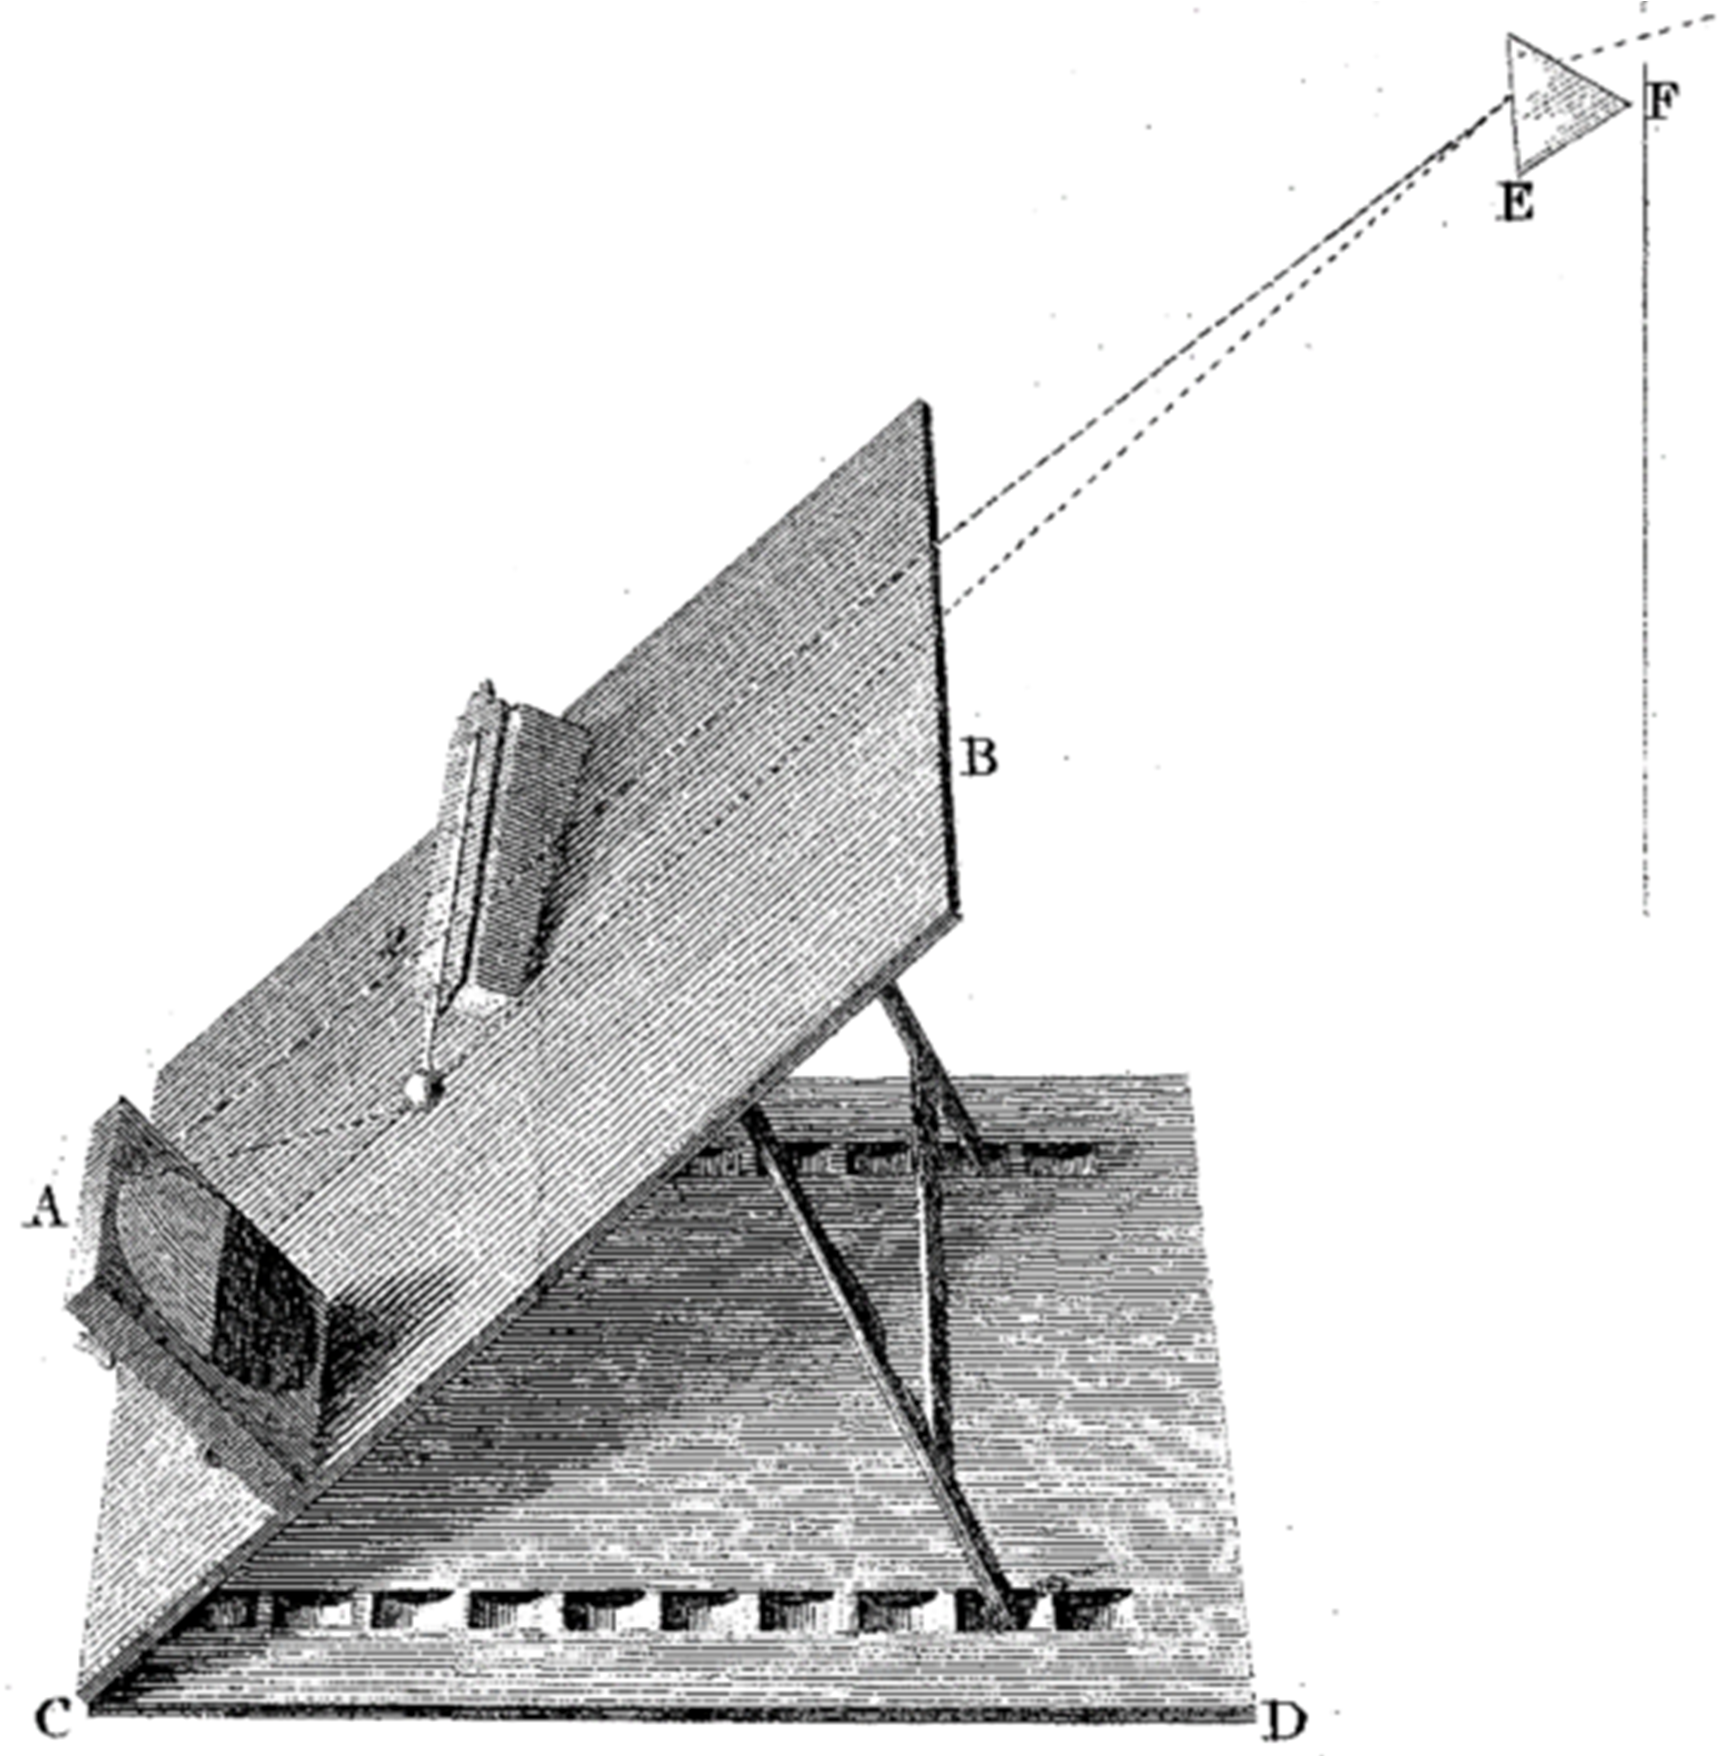
\includegraphics{figs/fundamentals/herschel_decomposition.png}
	\caption{Measurement stand for reading temperature from radiation with a single thermometer \cite{minkina_how_2021}.}
	\label{fig:herschel_decomposition}
\end{marginfigure}
\begin{marginfigure}[7cm]
	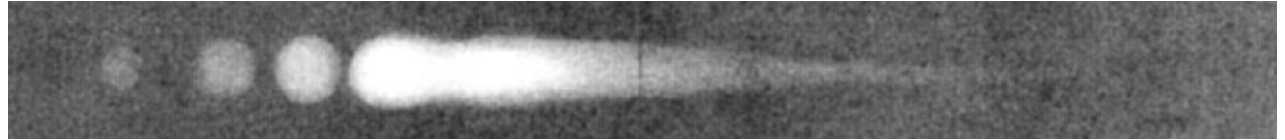
\includegraphics{figs/fundamentals/infrared_absorption.png}
	\caption{Example of thermogram originated from a wet piece of paper and targetted radiation.}
	\label{fig:infrared_absorption}
\end{marginfigure}
\begin{kaobox}[frametitle=Discovery of infrared radiation]
The heat was initially believed to only transfer through matter until the experiments of William Herschel led to the discovery of 'calorific' or 'invisible' rays. This term referred to wavelengths that fall beyond the red spectral interval end and thus are invisible to the naked eye. Circa 1737, Châtelet suggested that different colours could carry different temperatures, though it would not be until 1800 that this theory was proved. W. Herschel passed the Sun's radiation through a prism and placed mercury thermometers over the split spectrum. The measured temperatures not only differed from atmospheric temperature but also the readings beyond the red end were higher. A more advanced set-up of this experiment is shown in Figure \ref{fig:herschel_decomposition}, with a reflective mirror and a platform that can vary its slope \cite{ring_discovery_2000, minkina_how_2021, minkina_infrared_2009}. Later in 1804, John Leslie checked the discrepancies in the temperature readings of different materials, using the so-called Leslie cube. Another curious experiment showed that there exist atmospheric windows with a higher transmission factor and less absorption. W. Herschel's son, John Herschel, used the technique called evaporography to create a thermal image, also known as a thermogram, over a wet piece of paper. The result is shown in Figure \ref{fig:infrared_absorption}, with white dots representing beyond infrared wavelengths. 
\end{kaobox}

\acrshort{ir} radiation is physically represented as electromagnetic (\acrshort{em}) waves that propagate through space as a sinusoidal function ($f(x) = k \cdot \sin{x}$) with a spatial periodicity, known as wavelength (\si{\meter}), $\lambda$, and a period of oscillation (\si{\second}), $\mathcal{T}$. 
%The speed of propagation depends on the kind of wave and is calculated with the frequency $\nu$ derived from $\mathcal{T}$ and $\lambda$. However, EM waves are known to propagate at the speed of light ($c = 300 000\si{\kilo\meter}^{-1}$) in a vacuum; otherwise, $c$ depends on the index of refraction of the medium of propagation. 
Waves are affected by disturbance, and according to this can be organized into longitudinal and transverse waves, with both being perpendicular. Transverse waves can oscillate in many different directions, which yields the concept of polarization and plane of polarization. The latter is defined through the direction of propagation and the disturbance. If a wave is categorized as unpolarized, then the plane of polarization can adopt all possible orientations. Regarding \acrshort{ir} radiation, it is perturbed by electric and magnetic fields, and its polarization is expressed through the electric field and the direction of propagation ($x-z$ plane). Therefore, the recording of waves and \acrshort{ir} radiation can be performed by polarizers, with a simple microscopically small conducting grid being sufficient for filtering out waves that are non-perpendicular to such a grid \cite{vollmer_infrared_2017}. In thermography, the captured \acrshort{em} radiation is referred to \textbf{thermal radiation}, emitted by bodies at a temperature over 0 \si{\kelvin} (-273.15ºC). 

The radiation measured from a surface is not solely affected by such a surface, but other factors intervene in the acquisition. Among these, the most notable factors are the absorption and scattering phenomena from atmospheric particles and sensor components, as well as the radiation emitted by surrounding objects and the atmosphere. The degree of transmissivity of the atmosphere, which may vary throughout time, is known as the transmission factor. Other minor influencing factors are the distance to the sensor, the object's emissivity, dimensions and shape, the atmospheric temperature and humidity as well as the temperature of optics \cite{vollmer_infrared_2017}. 

Although the \acrshort{ir} spectrum covers a wide range of wavelengths (see Figure \ref{fig:introduction_scheme}), \acrshort{ir} imaging is focused on a small part of these. Three spectral ranges are the most frequent in thermography: short-wave infrared (\acrshort{swir}: 900-1,700 \si{\nano\meter}), mid-wave infrared (\acrshort{mwir}: 3,000-5,000 \si{\nano\meter}) and long-wave infrared (\acrshort{lwir}: 8,000-14,000 \si{\nano\meter}) \cite{gade_thermal_2014, vollmer_infrared_2017}. Commercial sensors are available on the three spectral ranges; whether one of them ought to be used over another must attend to criteria such as atmospheric transmission, expected radiation and the physics of detectors. A simple Scopus search shows that \acrshort{mwir} imaging is the most widespread, though it is significantly downgraded over \acrshort{swir} and \acrshort{lwir} for \acrshort{uas} platforms. Figure \ref{fig:infrared_scopus} shows the percentage of work devoted to each \acrshort{ir} interval. The Scopus searches were the following: $(\mathtt{thermographic} \lor \mathtt{thermography} \lor \mathtt{thermal} \lor \mathtt{infrared} \lor \mathtt{ir}) \land (\mathtt{drone} \lor \mathtt{uav} \lor \mathtt{uas}) \land ((x-\mathtt{wave} \lor y\mathtt{WIR}))$, with $x$ being short ($y \gets $S), mid ($y \gets $M) or long ($y \gets $L). In this dissertation, the integrated thermographic camera operates over the \acrshort{lwir} range. 

\begin{figure}[ht]
	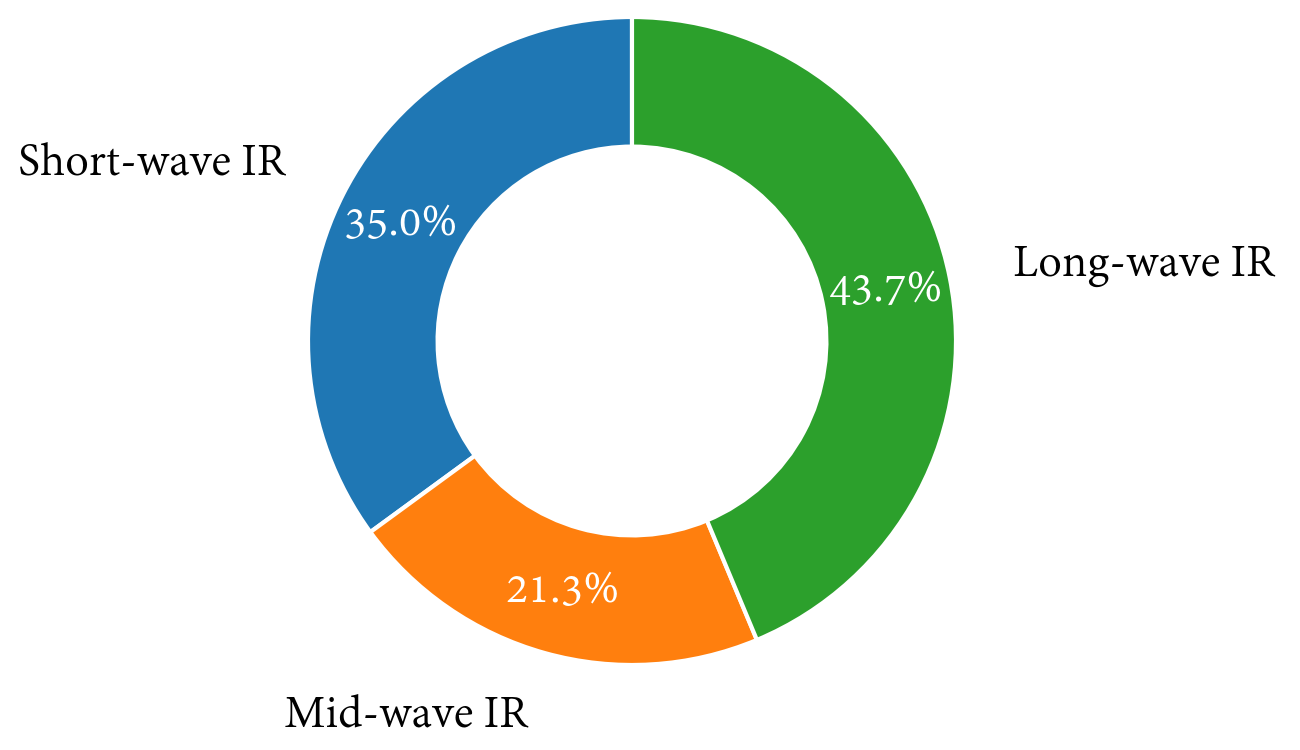
\includegraphics[width=.75\textwidth]{figs/fundamentals/infrared.png}
	\caption{Number of manuscripts related to different \acrshort{ir} intervals.  }
    \label{fig:infrared_scopus}
\end{figure}

Preferences on the \acrshort{lw} range over \acrshort{swir} and \acrshort{mwir} are not a casualty, but it is rather influenced by atmospheric transmissivity. Most of Earth's surface has its emission peak in this interval, while the \acrshort{lw} range is also known as an atmospheric window where absorption is considerably smaller \cite{gonzalez_thermal_2019, quattrochi_thermal_1999}. 

An exhaustive, though not complete, list of the most frequent commercial \acrshort{ir} cameras used for research is shown in Table \ref{table:thermographic_devices}. Every single of them is designed for measuring \acrshort{lwir}, while their focal length is typically over 13 \si{\milli\meter}. Instead of widening the camera view, these devices acquire images focused on very specific areas with a very small image resolution. Therefore, the mentioned drawbacks ought to be considered to make an appropriate flight plan. For instance, side overlapping among different sweeps from the planned trajectory must be large enough to guarantee there exists overlapping between thermal imagery. 

\renewcommand{\arraystretch}{1.2}
\begin{table*}[htb]
    \small
    \caption{Consumer-grade thermal devices found in the literature and their specifications, according to the manufacturer's datasheets.}
    \label{table:thermographic_devices}
    \begin{tabular}{llllll}
        \toprule
        Thermographic tool & Focal length & FOV & Image res. & Spectral range & Ref. work \\
        \midrule
        \multicolumn{6}{c}{DJI}\\
        \multirow{2}{*}{Zenmuse XT2}    & 13 \si{\milli\meter}   & $32^{\circ} \times 26^{\circ}$  & $640 \times 512$ px  & \multirow{2}{*}{LWIR (7.5 - 13.5 \si{\micro\meter})}    & \multirow{2}{*}{\cite{lopez_optimized_2021, yuan_uav-based_2021, jo_dense_2021}}\\
        & 19 \si{\milli\meter}   & $25^{\circ} \times 19^{\circ}$  & $336 \times 256$ px  &   & \\
        Zenmuse H20T     & 13.5 \si{\milli\meter}   & $31.7^{\circ} \times 25.36^{\circ}$  & $640 \times 512$ px  & LWIR (8 - 14 \si{\micro\meter})    & \cite{paziewska_integration_2022, jiang_diurnal_2022}\\
        \cmidrule{1-6}
        \multicolumn{6}{c}{FLIR}\\
        FLIR A320     & 18 \si{\milli\meter}   & $25^{\circ} \times 18.8^{\circ}$  & $320 \times 240$ px  & LWIR (7.5 - 13.5 \si{\micro\meter})    & \cite{guilbert_fusion_2020}\\
        FLIR A35     & 9 \si{\milli\meter}   & $48^{\circ} \times 39^{\circ}$  & $320 \times 256$ px  & LWIR (7.5 - 13.5 \si{\micro\meter})    & \cite{comba_2d_2019}\\
        FLIR One     & 15 \si{\centi\meter}   & $50^{\circ} \times 38^{\circ}$  & $80 \times 60$ px  & LWIR (8 - 14 \si{\micro\meter})    & \cite{javadnejad_photogrammetric_2020}\\
        FLIR A65     & 25 \si{\milli\meter}   & $25^{\circ} \times 20^{\circ}$  & $640 \times 512$ px  & LWIR (7.5 - 13.5 \si{\micro\meter})    & \cite{adan_fusion_2017, jarzabek-rychard_supervised_2020, lin_fusion_2019, westfeld_generation_2015}\\
        FLIR Tau2 640     & 13 \si{\milli\meter}   & $45^{\circ} \times 37^{\circ}$  & $640 \times 512$ px  & LWIR (7.5 - 13.5 \si{\micro\meter})    & \cite{boesch_thermal_2017, sledz_thermal_2018}\\
        \cmidrule{1-6}
        \multicolumn{6}{c}{Sensefly}\\
        Sensefly thermoMAP     & N.A.   & N.A.  & $640 \times 512$ px  & LWIR (7.5 - 13.5 \si{\micro\meter})    & \cite{padua_vineyard_2019}\\
        \bottomrule
    \end{tabular}
\end{table*}
\renewcommand{\arraystretch}{1}

\subsection{Hyperspectral imaging}

Hyperspectral imaging (\acrshort{hsi}) differs from multispectral imaging in the number of bands, wavelengths and bandwidth of these. Hyperspectral images are 3D data cubes known as \textbf{hypercubes}, where each pixel is defined within a continuous spectrum range (Figure \ref{fig:fundamentals_material_hyperspectral}). The spectral resolution is typically given in \si{\nano\meter} or as a number of bands, though the second is preferred as the resolution can vary throughout the covered interval. Spectral signatures are complete and differentiable over the observed wavelength range, and thus, hypercubes outperform discrete multispectral data on the classification, segmentation and unmixing of materials. For instance, different varieties of plants might have a radiative response too similar among them, even using \acrshort{hsi}. Therefore, \acrshort{ai} algorithms could be applied to the automatic detection of the most discriminative wavelengths and be accordingly weighted to provide a meaningful result from input data. 

Unlike other imaging tools, \acrshort{hsi} has undergone a rising path from major to minor; from satellite scanning to \acrshort{uas} and laboratory applications. Hence, it is applied in a wide range of applications, from phenotyping, cultural heritage, medical research and food processing to biochemistry and the monitoring of Earth's processes and areas of interest, among others \cite{amigo_hyperspectral_2019}. Also in contrast to multispectral imaging, preprocessing on \acrshort{hsi} is still very frequently investigated. 

Remotely sensed data is affected by several factors, including acquisition conditions and random errors caused by sensors as well as atmospheric and surface effects. Radiometric correction over \acrshort{hsi} has been conducted to obtain representative data from the Earth's surfaces. The bibliography on this field has covered many topics, though it is mainly focused on satellite imaging. While some of the studied techniques can be applied to \acrshort{uas} imaging, other chapters are irrelevant to our target platforms, \acrshort{uas}. For instance, atmospheric effects such as absorption are of no interest in close-range work. However, the low flight altitude, the \acrshort{uas} instability or its viewing angle harden the pre-processing operations \cite{jakob_need_2017}. Geometric and radiometric corrections as well as spectral calibrations are also required to obtain accurate data \cite{adao_hyperspectral_2017}. Geometric distortions refer to those defects caused primarily by the \acrshort{uas} instability as well as due to the acquisition technique. For instance, push-broom sensors present higher geometric distortions that can be reduced by means of stabilizers. Geometric correction can be achieved with an \acrshort{imu}, a \acrshort{gps} as well as a Digital Elevation Model (\acrshort{dem}). Although there exists commercial software based on this approach, it requires a high-precision system for obtaining accurate corrections. Instead, Ground Control Points (\acrshort{gcp}) have been extensively used to ensure correct positioning \cite{ramirez-paredes_low-altitude_2016}. Also, the dual acquisition of visible and hyperspectral imagery allows matching both data sources \cite{jurado_efficient_2021, xue_compact_2021, ramirez-paredes_low-altitude_2016}, with the visible data being geometrically correct. Alternatively, feature matching among overlapping images has also been shown to help with geometric correction \cite{akhoundi_khezrabad_new_2022}.

\begin{figure}[ht]
	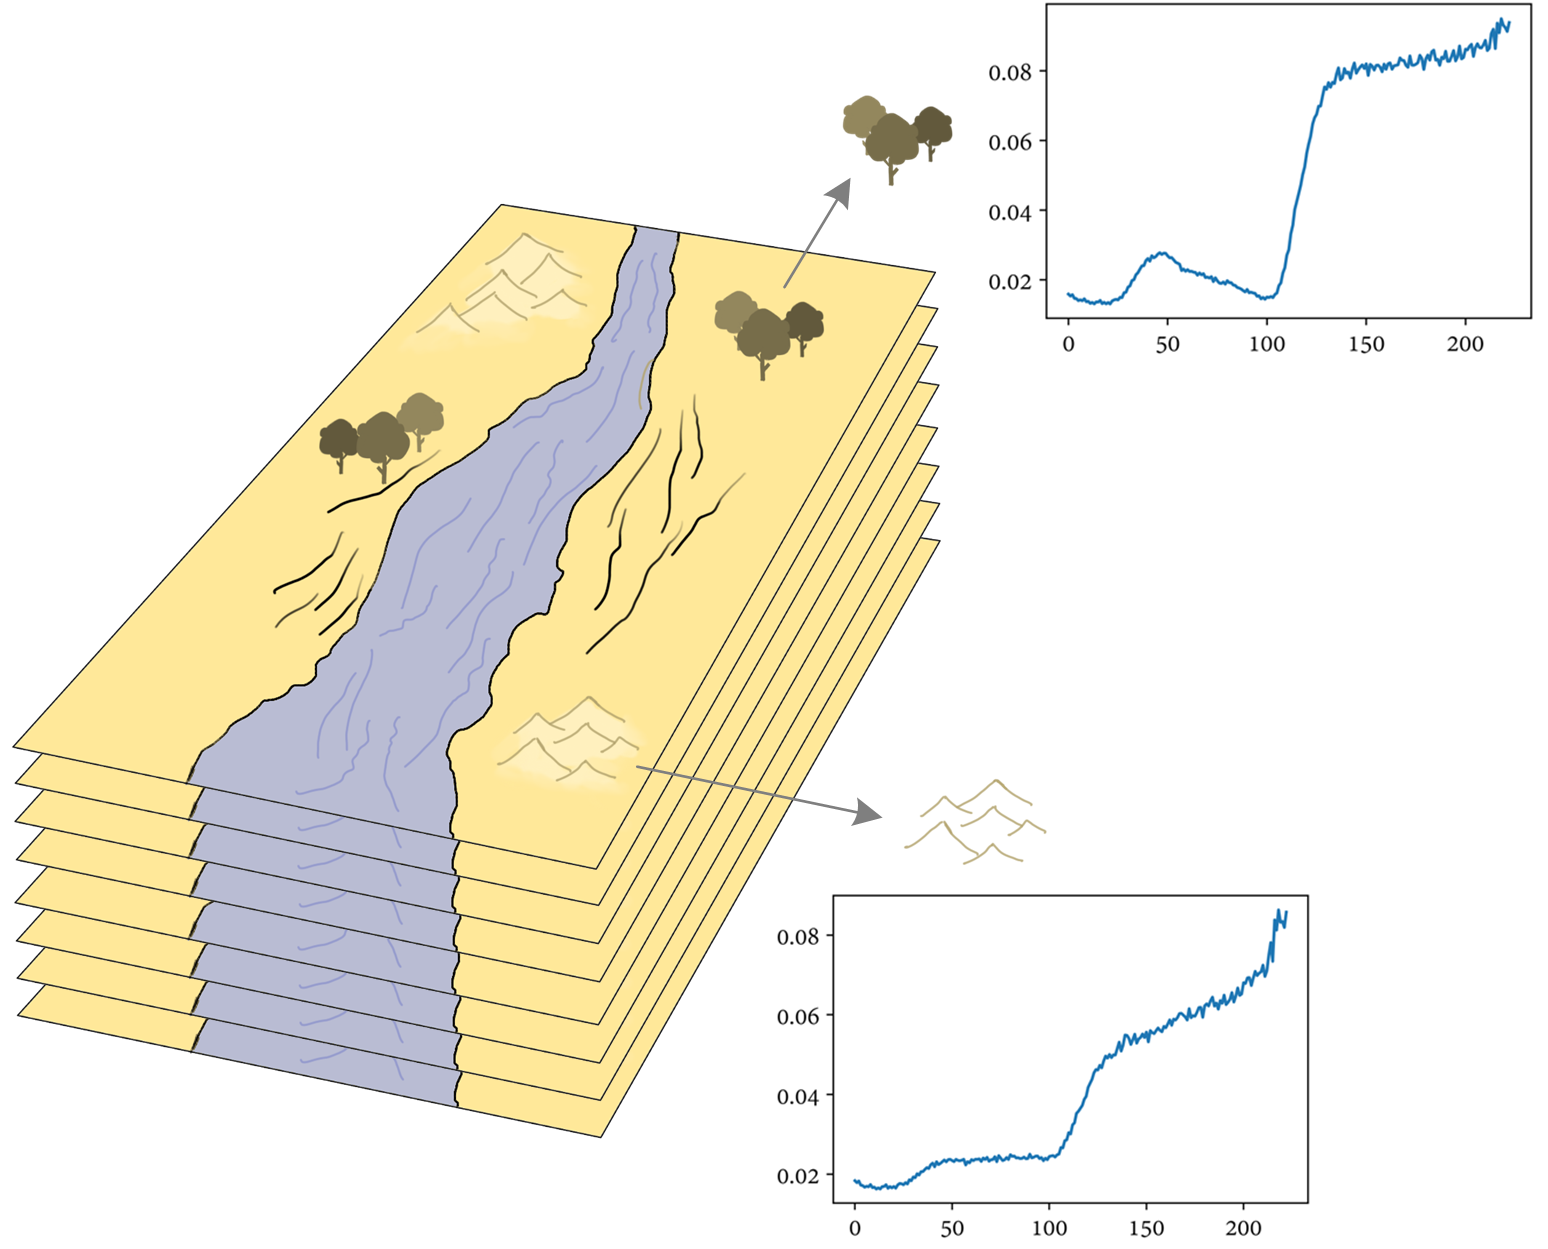
\includegraphics[width=.9\textwidth]{figs/fundamentals/material_hyperspectral.png}
	\caption{Scheme of hyperspectral images, where vegetation and ground surfaces have a different spectral signature.  }
    \label{fig:fundamentals_material_hyperspectral}
\end{figure}

Similarly to geometric distortions, radiometric defects can be corrected with software tools from the hyperspectral manufacturer. The objective is to transform the sensor's \acrshort{dn} to radiance, influenced by acquisition conditions, and reflectance, regardless of previous conditions. To this end, the coefficients needed for this correction are typically calibrated in the laboratory. However, they are more likely to vary through time \cite{adao_hyperspectral_2017}, thus leading to worsening the radiometric correction. This process can be supported by the use of grayscale tarps whose reflectance is known, thereby allowing to perform linear interpolations to calibrate the acquired \acrshort{dn} \cite{lucieer_hyperuasimaging_2014} with the Empirical Line Method (\acrshort{elm}) \cite{aasen_quantitative_2018, sousa_uav-based_2022}. Dark and grey/white references are required to perform this linear interpolation \cite{jakob_need_2017, sagan_data-driven_2022, duan_land_2013}, typically from isotropic materials (near to Lambertian) that present a grayscale palette. Alternatively, the acquisition of radiance samples can help to transform \acrshort{dn}s with fitting methods such as the Least-Square Method (\acrshort{lsm}). Sensor-based factors, including the vignetting effect that causes a drop in the intensity, lead to a different radiometric response in pixels of the same bands \cite{yang_dom_2017}.

Atmospheric corrections have also been documented for \acrshort{uas} flights. Accordingly, the at-sensor radiance can be correlated to the surface Hemisphe\\rical-Directional Reflectance Function (\acrshort{hdrf}) measured in the laboratory beforehand. The previous grayscale palette with Lambertian materials can be used to achieve this \cite{lucieer_hyperuasimaging_2014}. Physically-based methods have also been investigated by measuring the atmospheric conditions that conditioned the hyperspectral imaging, though they are more time-consuming. Finally, some public repositories offer atmospherically corrected datasets, e.g., the Aviris data portal \cite{california_institute_of_technology_aviris_nodate}, whereas widespread software for hyperspectral processing also includes semi-automatic correction algorithms (ENVI, Headwall SpectralView, etc). Other studies calculate the Bidirectional Reflectance Distribution Function (\acrshort{brdf}) of visible materials. Previous corrections are applied, and \acrshort{brdf} kernels are estimated using kernels such as Ross and Li from the varying response of materials according to solar and view angles \cite{queally_flexbrdf_2022, jia_kernel-driven_2020, sagan_data-driven_2022}.

The list of hyperspectral sensors on the market that can be coupled with \acrshort{uas} has significantly increased in recent years. Therefore, Table \ref{table:hyperspectral_devices} solely illustrates those that provide higher spectral resolution and have been explored in the hyperspectral state-of-the-art literature. As previously regarded, the spectral range can be calculated from the spectral resolution, in \si{\nano\meter}, and the number of bands. However, as observed in Table \ref{table:hyperspectral_devices}, this is not exactly right for every sensor as the spectral resolution may not be constant. In this dissertation, the research focused on hyperspectral imaging operates over data cubes from Headwall Photonics Inc.\textregistered Nano HyperSpec, with sampling intervals ranging from 2.2 \si{\nano\meter} to 6 \si{\nano\meter} in the central wavelengths.

\renewcommand{\arraystretch}{1.2}
\begin{table*}[h]
    \small
    \caption{Hyperspectral sensors found in the literature and their specifications, according to the manufacturer's datasheets.}
    \label{table:hyperspectral_devices}
    \begin{tabular}{lllllll}
        \toprule
        Tool & Spectral range & \#Bands & Spectral res. & Acquisition & Spatial res. & Ref. work \\
        \midrule
        \multicolumn{7}{c}{Headwall Photonics}\\
        Nano HyperSpec & 400-1000 \si{\nano\meter}   & 272-775 & 6 \si{\nano\meter}  & Push-broom    & 640 px  &\cite{sankey_uav_2018, sousa_uav-based_2022}\\
        Micro Hyperspec & 400-1000 \si{\nano\meter}   & 837-923 & 2.5 \si{\nano\meter}  & Push-broom    & 1004 px  &\cite{sousa_uav-based_2022}\\
        \cmidrule{1-7}
        \multicolumn{7}{c}{SENOP}\\
        VIS-VNIR Snapshot & 400-900 \si{\nano\meter}   & 380 & 10 \si{\nano\meter}  & Snapshot    & $1010\times1010$ px & \cite{sousa_uav-based_2022}\\
        HSC-2 & 450-900 \si{\nano\meter}   & Up to 1000 & 6-18 \si{\nano\meter}  & Snapshot    & $1024\times1024$ px & \cite{sousa_uav-based_2022}\\
        \cmidrule{1-7}
        \multicolumn{7}{c}{XIMEA}\\
        XIMEA SNm4x4 & 460-600 \si{\nano\meter}   & 16 & 15 \si{\nano\meter}  & Snapshot    & $512\times272$ px & \cite{gao_cbff-net_2023}\\
        \cmidrule{1-7}
        \multicolumn{7}{c}{Specim}\\
        AISA Angle & 400-970 \si{\nano\meter}   & 488 & 2.9 \si{\nano\meter}  & Pushbroom    & $1024$ px & \cite{windrim_unsupervised_2023}\\
        FX17 & 900-1700 \si{\nano\meter}   & 224 & 8 \si{\nano\meter}  & Pushbroom    & $640$ px & \cite{sousa_uav-based_2022}\\
        \cmidrule{1-7}
        \multicolumn{7}{c}{Cubert GmbH}\\
        UHD 185 Firefly & 450-950 \si{\nano\meter}   & 125 & 8 \si{\nano\meter}  & Snapshot    & $1000\times1000$ px & \cite{yue_comparison_2018}\\
        \bottomrule
    \end{tabular}
\end{table*}
\renewcommand{\arraystretch}{1}

\subsection{Active sensing}

Active systems, unlike previous passive sensors, provide their own energy source and therefore do not rely on external light sources, radiation emitted and reflected by surfaces and weather conditions \cite{dong_lidar_2018}. Among active sensors, the focus of this dissertation is on \acrshort{lidar}. It is an optical remote sensing technique that measures the properties of scattered light and can be used on spaceborne, airborne and ground-based platforms. The emitted energy is bounced back after colliding on the Earth's surfaces, thus being capable of determining distances by measuring the time delay between emission and reception, the so-called Time of Flight (\acrshort{tof}). It is also aimed at measuring speed (wind \acrshort{lidar}) and attenuation of volume targets such as the atmosphere or seawater \cite{emery_introduction_2017}. The emitted electromagnetic energy operates at a wavelength, with \acrshort{lidar} working at much shorter wavelengths than radar, typically in atmospheric transmission windows. Some of these were previously reviewed (infrared), although \acrshort{lidar} systems also operate at the visible and ultraviolet (\acrshort{uv}) spectral range. This parameter determines which is the minimum size of objects to be detected, with shorter wavelengths being more sensitive to smaller particles. Hence, \acrshort{lidar} systems are typically used for atmospheric and meteorology research. Backscattering is dependent on the dielectric discontinuity produced by collided surfaces, and therefore, nonmetallic objects have significantly lower responses to higher wavelengths \cite{dong_lidar_2018}. 

A simplification of \acrshort{lidar} emissions is the concept of ray: $r(t) = o + \vec{d}t$. This is a geometric data type defined by the starting position, $o$, and a direction vector, $\vec{d}$, that infinitely spread in the space. Unlike rays in Computer Graphics (\acrshort{cg}), \acrshort{lidar} emit volumetric beams whose targets are surface areas rather than points. Therefore, impacts on surfaces may not entirely block these beams, thus leading to penetrating surfaces that harden the visualization of objects below it but are not completely enclosed. For example, \acrshort{lidar} has been applied to archaeology with notable results since it allows removing points from high-density forests to uncover remains at the Earth's surface. Other widespread applications of \acrshort{lidar} technology are in \acrshort{rs}, geology, atmospheric physics or seismology \cite{emery_introduction_2017}. More specific ones concerning our work are building inspections \cite{shariq_revolutionising_2020}, monitoring of natural environments (landform dynamics \cite{guisado-pintado_3d_2019}, ecological resilience \cite{mitasova_geospatial_2010}, etc.), autonomous driving \cite{kuutti_survey_2021}, preservation of cultural heritage \cite{andriasyan_point_2020}, land mapping or urban planning \cite{zhou_street-view_2022}.

Similar to previous optical sensors, \acrshort{lidar} sensors are also influenced by factors such as the local incidence angle between the surface normal and beams, $\gamma$, and the dielectric properties of materials, expressed as $\varepsilon = \varepsilon' + j\varepsilon''$, with the dielectric constant depending on the permittivity ($\varepsilon'$) and the loss factor (the imaginary part, $\varepsilon''$). Other major factors are polarization, i.e., the orientation of the transmitted electromagnetic vectors, and the surface roughness.

Most common \acrshort{lidar} operates on the 600-1000 \si{\nano\meter} spectral range for non-scientific applications; ground-based are frequently in 500-600 \si{\nano\meter}, whereas airborne systems work over 1000-1600 \si{\nano\meter}. The second is of special interest for this dissertation and thus we will stick to it. Despite being more expensive, these are also eye-safe due to working at larger wavelengths. Nevertheless, most commercial sensors operating below 1000 \si{\nano\meter} are eye-safe nowadays. Airborne \acrshort{lidar} can record several discrete measurements per emitted pulse, or record a signal sampled with a frequency determined by time interval or distance (for example, sampled every 1 \si{\nano\second} or 15 \si{\centi\meter}). The latter is known as full-waveform \acrshort{lidar} and is mainly used in forestry applications since it provides a signature that helps on estimating the density at different height levels. On the other hand, discrete-return \acrshort{lidar} has found a wider number of applications. A minimal operative \acrshort{lidar} is composed of laser and receiver units, \acrshort{gps} and \acrshort{imu} systems and control, monitoring and recording units. Hence, one of the main shortcomings of imagery is overcome by \acrshort{lidar}, as recorded 3D points are georeferenced. 
\begin{gather}
    \label{eq:lidar_distance}
    \begin{aligned}
        R &= \frac{1}{2}ct_s
    \end{aligned}
\end{gather}

Equations \ref{eq:lidar_distance} and \ref{eq:lidar_equation} may shed some light on the functioning of \acrshort{lidar} systems. First, the distance of the surface that returned the backscattered energy, $R$, is calculated according to the time delay, $t_s$, and the speed of light, $c$. Also, the acquired energy, involving both emitter and receiver, is expressed as shown in Equation \ref{eq:lidar_equation}. There are multiple formulae in the literature to represent how is \acrshort{lidar} intensity retrieved, though most are analogous \cite{hofle_correction_2007, bolkas_effect_2018, dong_lidar_2018}.
\begin{gather}
    \label{eq:lidar_equation}
    \begin{aligned}
        \sigma &= \frac{4\pi f_{r}(\vec{w})A_{t}}{\Omega}\\
        A_{t} &= \frac{\pi R^{2} \beta^{2}_{t}}{4}\\
        P_{r} &= \frac{\bar{I} D^{2}_{r} \eta_{atm} \eta_{sys} \sigma}{4 \pi R^{4}}=
        \frac{4\pi^2 \bar{I} D^{2}_{r} \eta_{atm} \eta_{sys}  f_{r}(\vec{w})}{4\Omega R^{2} \beta^{2}_{t}}
    \end{aligned}
\end{gather}
where $\bar{I}$ is the emitted energy, $D^{2}_{r}$ is the receiver diameter (\si{\meter}), $\eta_{atm}, \eta_{sys}$ are atmospheric and system transmission factors, $f_{r}(\vec{w})$ is the target reflectance, $A_{t}$ is the target area, $R$ is the distance to receiver in \si{\meter}, $\beta$ is the transmit beam width (\si{\radian}) and $\Omega$ is the scattering solid angle (\si{\steradian}). $\pi$ controls the amount of energy spreading a specific point since it spreads in every possible direction within a semisphere.

Lasers are the main unit in \acrshort{lidar} systems, and energy emitted by these can be oriented through a scanning deflector to output different scanning patterns, as depicted in Figure \ref{fig:lidar_patterns}. If the orientation of lasers varies, so does the scanning pattern. The fundamental deflections are based on polygonal mirroring, which generates parallel scan lines and swinging mirrors with zig-zag patterns, thus achieving more point density at the line boundaries. Other deflections are fibre optics, which produce a similar output to polygonal mirroring despite changing beam transmission technology, and rotating slanted mirrors that generate elliptical shapes. Finally, Risley prism scanners such as DJI Livox have a different pattern for sampling surfaces with more density and longer integration times \cite{bechtold_helios_2016, winiwarter_virtual_2022}.

\begin{figure*}[ht]
	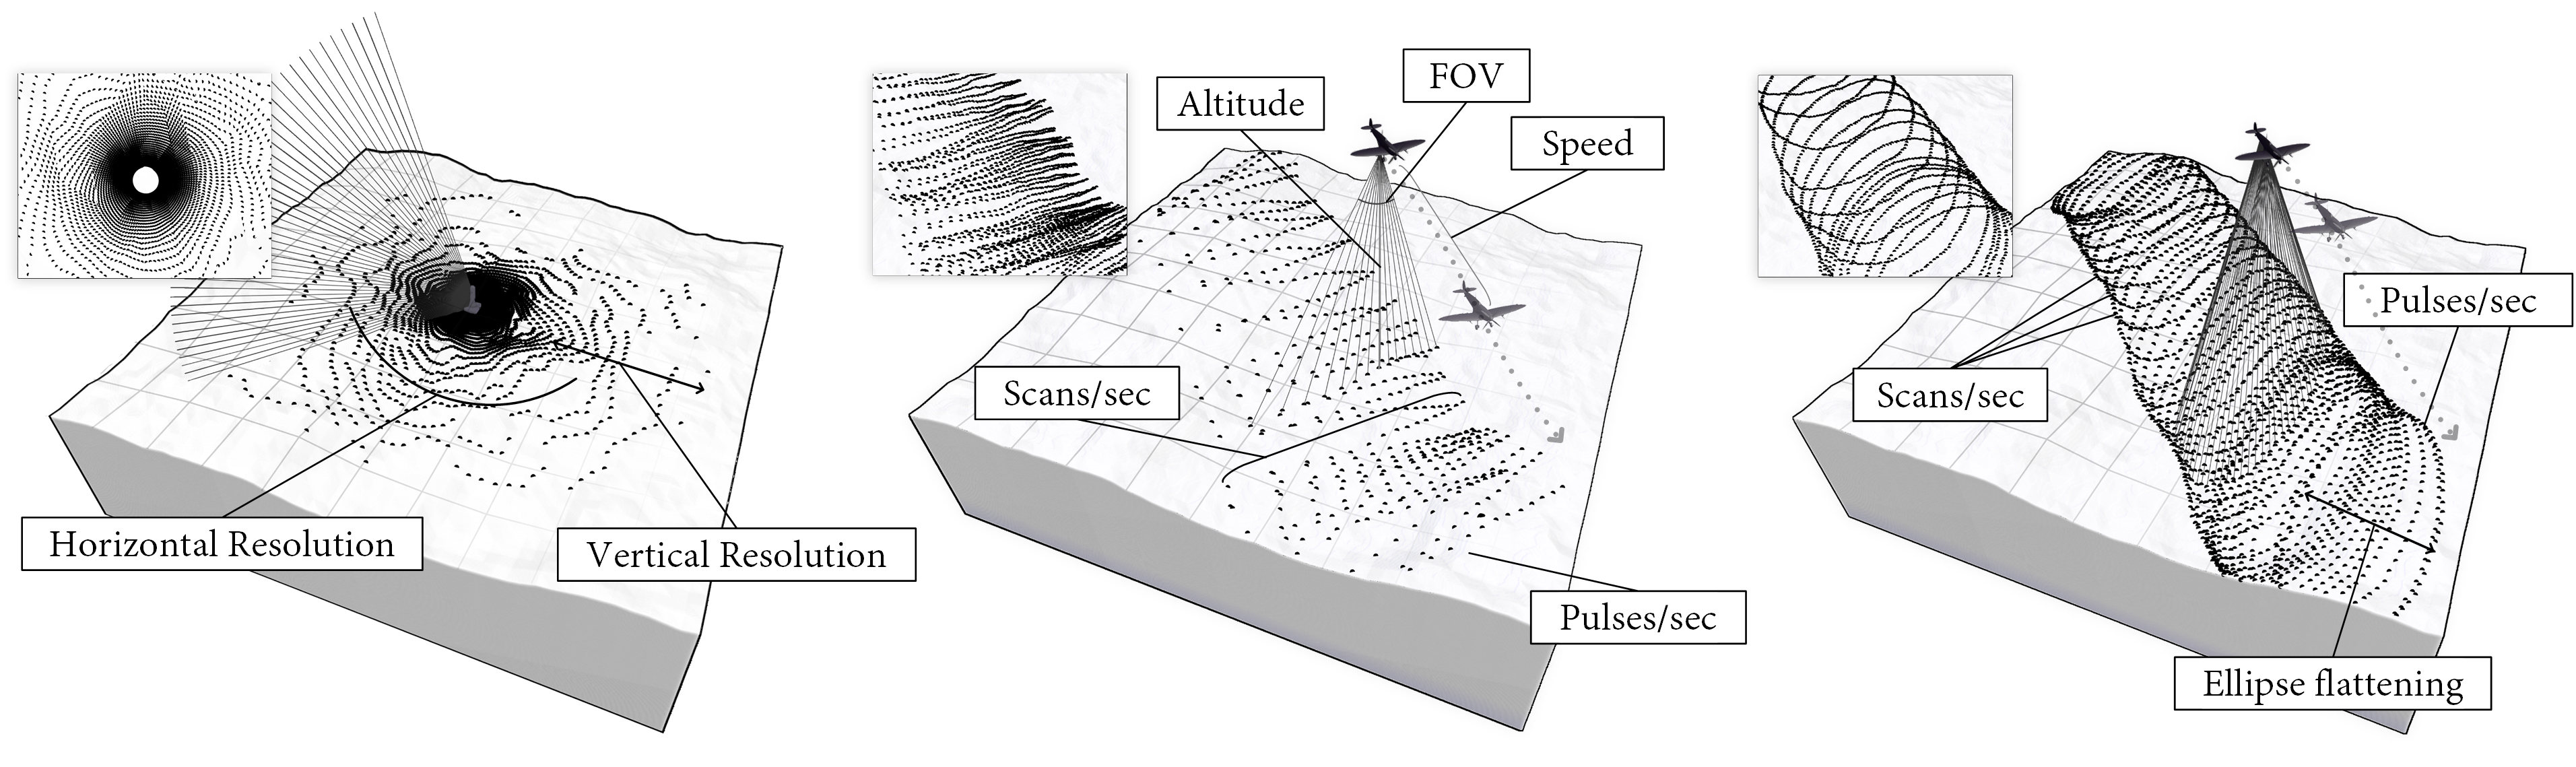
\includegraphics[width=\linewidth]{figs/fundamentals/lidar_patterns.png}
	\caption{Surveys performed with different path planning: a) the path is automatically computed according to the sensor's \acrshort{fov}, whereas in b) the path is drawn by the user, simplified using the Douglas-Peucker algorithm and subsampled using a Catmull-Rom spline. Zoomed-in images at the top-right corner show the effect of jittering. }
    \label{fig:lidar_patterns}
\end{figure*}

Table \ref{table:lidar_devices} shows a brief list of some widespread \acrshort{lidar} sensors, both terrestrial and airborne. It provides further insight into which are the most frequent wavelengths. Among these, \acrshort{lidar} sensors operating at 532 \si{\nano\meter} are also known as bathymetric and enable capturing shallow, underwater surfaces. Thus, it is especially relevant for hydrology and coastal monitoring.

\renewcommand{\arraystretch}{1.2}
\begin{table*}[ht]
    \small
    \caption{Most common \acrshort{lidar} systems in the literature and their attributes.}
    \label{table:lidar_devices}
    \begin{tabular}{lllllll}
        \toprule
        \acrshort{lidar} system & FOV & Echoes & Maximum range & Wavelength & Channels & Points/\si{\second} \\
        \midrule
        \multicolumn{7}{c}{Velodyne}\\
        HDL-32E    & $360^{\circ}\times41.3^{\circ}$    & 2   & 80-100\si{\meter} & 903\si{\nano\meter} & 32 & 1.39M\\
        Puck/Puck LITE    & $360^{\circ}\times30^{\circ}$    & 2   & 100\si{\meter} & 903\si{\nano\meter} & 16 & 600K\\
        Puck Hi-RES    & $360^{\circ}\times20^{\circ}$    & 2   & 100\si{\meter} & 903\si{\nano\meter} & 16 & 600K\\
        ULTRA Puck    & $360^{\circ}\times40^{\circ}$    & 2   & 100\si{\meter} & 903\si{\nano\meter} & 32 & 1.2M\\
        Alpha Prime    & $360^{\circ}\times40^{\circ}$    & 2   & 250\si{\meter} & 903\si{\nano\meter} & 128 & 4.8M\\
        \cmidrule{1-7}
        \multicolumn{7}{c}{Valeo}\\
        SCALA Gen 2    & $133^{\circ}\times10^{\circ}$    & 3   & 200\si{\meter} & 905\si{\nano\meter} & 16 & 25\si{\hertz}\\
        \cmidrule{1-7}
        \multicolumn{7}{c}{SICK}\\
        MRS1104C-111011    & $275^{\circ}\times7.5^{\circ}$    & 3   & 64\si{\meter} & 850\si{\nano\meter} & 32 & 165K\\
        \cmidrule{1-7}
        \multicolumn{7}{c}{Phoenix Systems}\\
        SCOUT-M2X   & $360^{\circ}\times40.3^{\circ}$    & 3  & 300\si{\meter} & 905\si{\nano\meter} & 32 & 640K\\
        SCOUT-32   & $360^{\circ}\times40^{\circ}$    & 2  & 220\si{\meter} & 905\si{\nano\meter} & 32 & 600K\\
        HydroRANGER   & $40^{\circ}$ VFOV  & 15  & 75\si{\meter} & 532\si{\nano\meter} & - & 200K\\
        RANGER-LR LITE   & $360^{\circ}$ HFOV  & 5  & 1000\si{\meter} & 1550\si{\nano\meter} & - & 1.5M\\
        \bottomrule
    \end{tabular}
\end{table*}
\renewcommand{\arraystretch}{1}

\subsection{Principles of physical measurement}

\acrshort{rs} covers a wide range of spectral wavelengths depicted in images that show the emitted and reflected radiation from the Earth's surfaces, including matter such as atmospheric particles and bare soil. A huge number of conditions and parameters are involved in the observed radiation, whose explanation would cover dozens of pages, if not a book. Hence, only a few remarks will be done here. 

A key ingredient in the understanding of the scene is the detailed specification of the appearance of materials regardless of light and the influence of other matter. Energy, as captured in nature, does not depict the underlying appearance of materials but the appearance when some specific circumstances are met. Therefore, measurements ought to be processed to make them independent from environmental and light conditions as well as surrounding surfaces. Not only it helps in the classification of materials present in the scene, given some reference spectral signatures, but also enables simulating lighting as occurs in real-world scenarios. For the latter, surfaces are assigned a spectral appearance that will not be rendered as so and thus will undergo changes as light and other matter interfere. 

Vollmer and Mollmann \cite{vollmer_infrared_2017} provided an exhaustive list of parameters conditioning the material emissivity, regardless of surrounding objects. Materials are the most differentiating feature, naïvely split into metal and nonmetal, where the latter are frequently returning higher emissivity. Also, the roughness level affects the outcome considerably; polished surfaces have lower emissivity and the contrary happens for rough surfaces. Further insight into energy dispersion helps to understand that it does not propagate over every direction of a semisphere with the same strength. Unlike blackbodies, which behave as perfect isotropic emitters, materials vary the emitted radiation conditioned to the outgoing direction. A key factor in this regard is the normal vector of the surface: the smaller the angle between the camera view direction and the normal vector, the higher the observed emissivity. However, this does not hold up for every material since conductors show the opposite behaviour. Similarly, the physical behaviour of light transport, including reflections, leads to increasing the emissivity for grooved surfaces as a consequence of rebounds. As will be observed throughout this dissertation, the spectral signature of materials is not constant, and therefore, some intervals are preferred over others in the seek of capturing a high emissivity from the target surfaces. For example, the \acrshort{nir} interval comprises the peak emissivity of vegetation. Finally, surface temperature also leads to slight emissivity changes.

\begin{figure}[ht]
	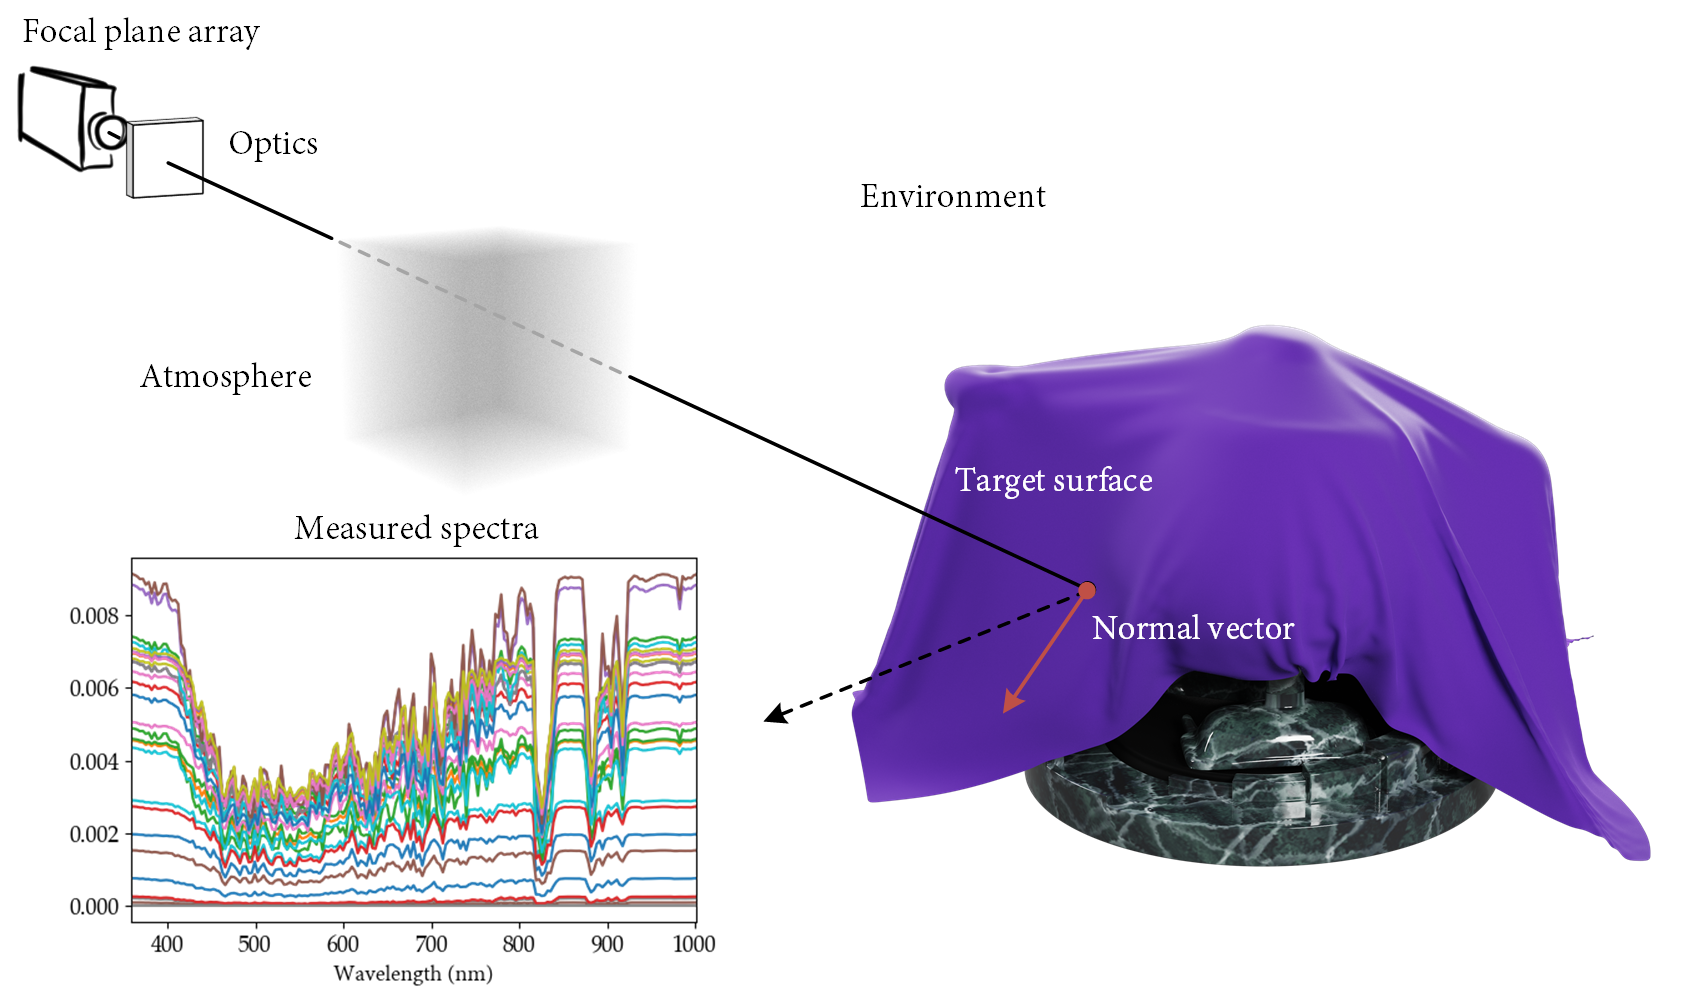
\includegraphics[width=.9\textwidth]{figs/fundamentals/physic_principles.png}
	\caption{Parameters that intervene in the measurement of radiance with a passive sensing tool. }
    \label{fig:physic_principles}
\end{figure}

\begin{marginfigure}[1cm]
	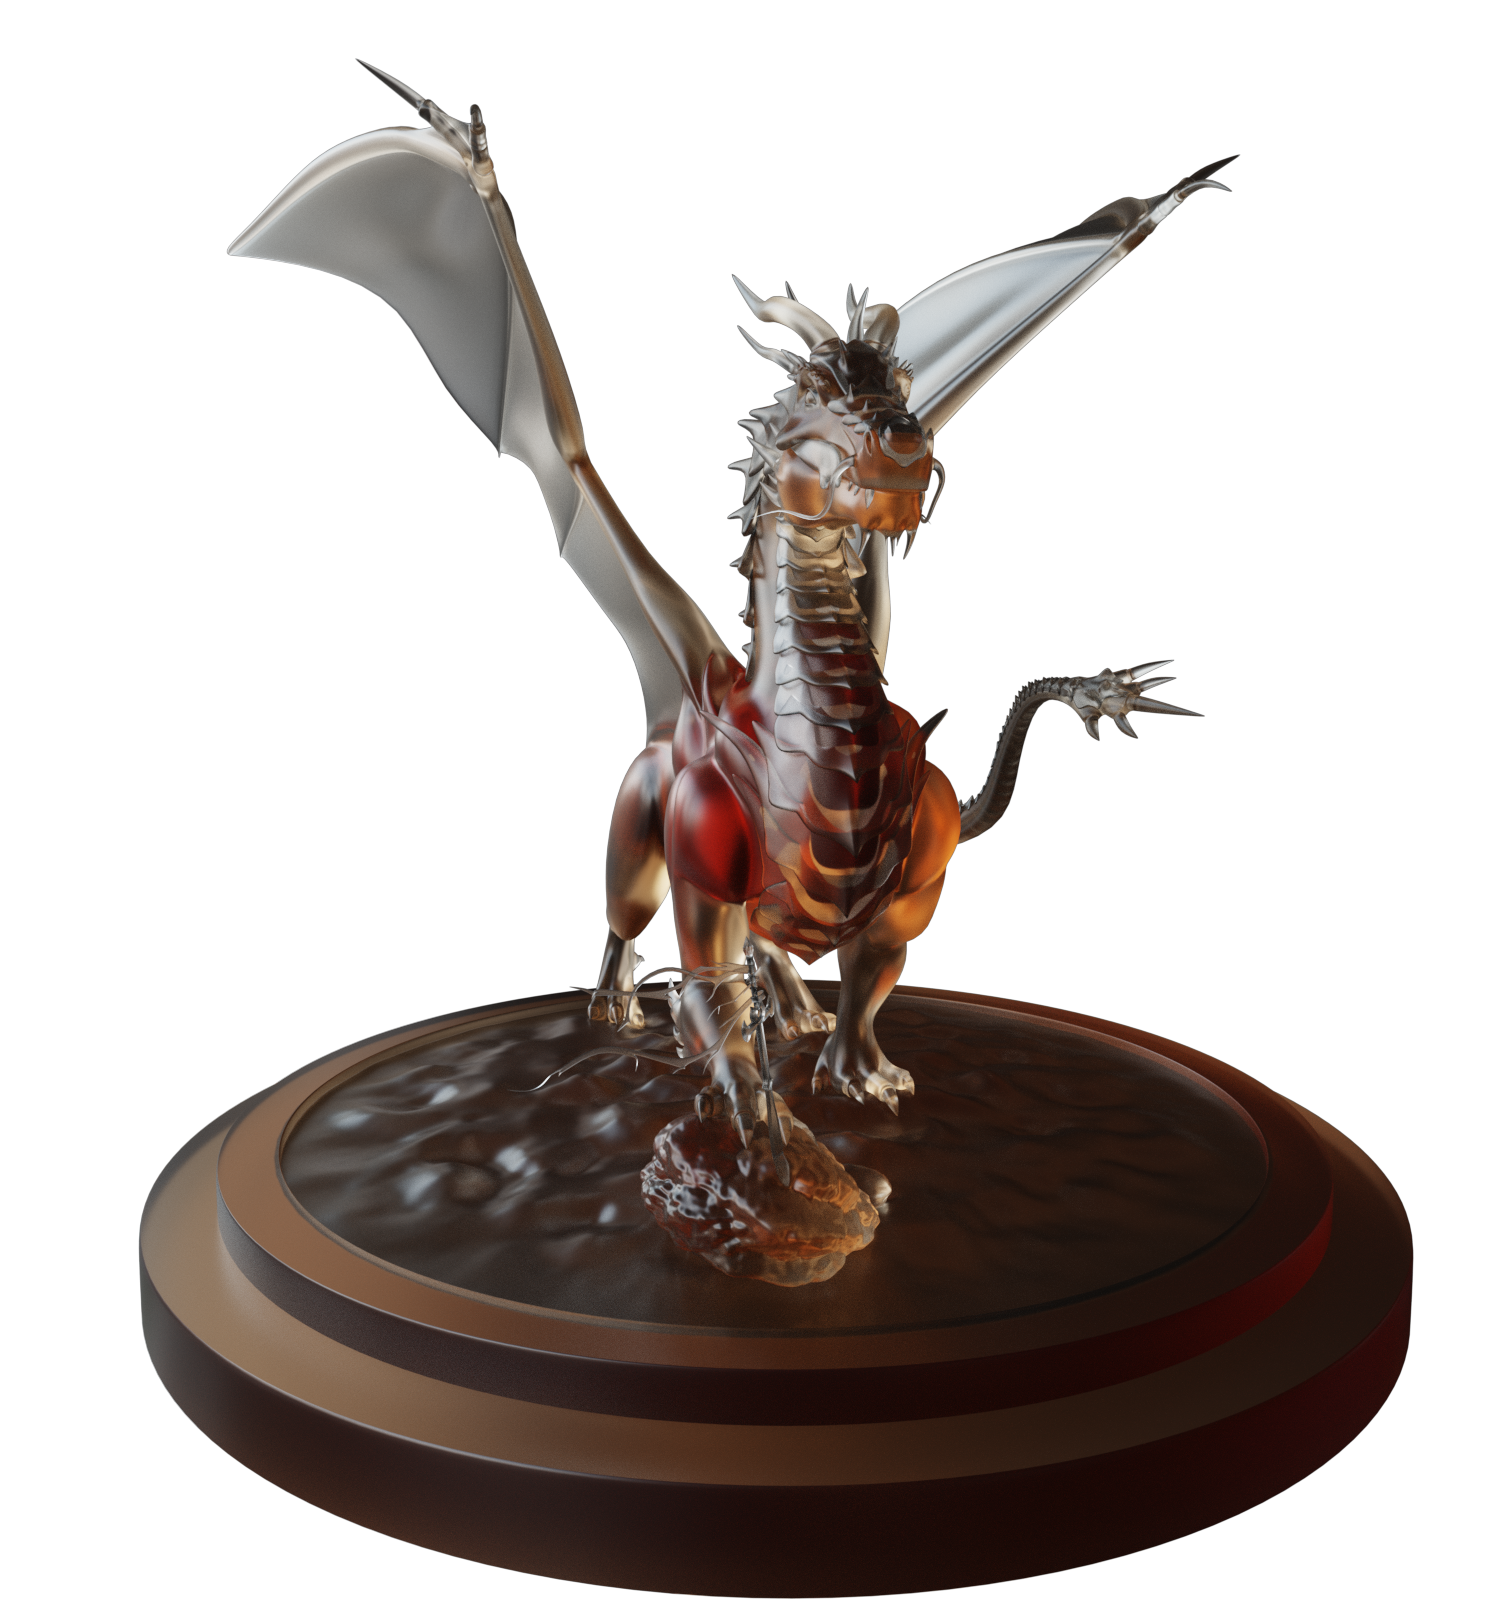
\includegraphics{figs/fundamentals/bssdf_2.png}
	\caption{Subsurface scattering simulated over a triangle mesh.}
	\label{fig:bssdf}
\end{marginfigure}
Radiometric measurements are layered data that can be carved to find the surfaces' spectral signatures. However, the carving process relies on corrections that are simple approximations considering a few of the mentioned factors rather than the overwhelming amount of uncontrolled attributes that can be found in nature. Otherwise, measurements can be performed with controlled surface features and lighting to provide databases of a wide range of materials \cite{dupuy_adaptive_2018}. Furthermore, databases on surface appearance comprise a number of discrete spectral signatures for each material, as these are typically parameterized by the input vector, $\omega_i$, and the output direction where radiance spreads, $\omega_o$ (Figure \ref{fig:brdf_wi_wo}). Otherwise, these vectors can be notated as local cartesian coordinates, half-angle difference parametrization and spherical coordinates, which are also very frequent \cite{montes_soldado_overview_2012}. The latter are expressed through four angles, $\varphi_i = \atan(y_i / x_i)$, $\varphi_o = \atan(y_o / x_o)$, $\theta_i = \acos(z_i)$ and $\theta_o = \acos(z_o)$. These functions, provisionally expressed as $f(\omega_i, \omega_i)$, parameterized with $\omega_i$, $\omega_o$, or their equivalent spherical coordinates, represent what was coined as Bidirectional Reflectance Distribution Functions (\acrshort{brdf}), or yet more intricate, Bidirectional Scatter Distribution Functions (\acrshort{bsdf}) and Bidirectional Scattering Surface Distribution Functions (\acrshort{bssdf}). Both \acrshort{bsdf} and \acrshort{bssdf} are aimed at simulating the indirect light transport from surrounding surfaces as well as their own surfaces. \acrshort{bssdf} are particularly hard to calculate as the entering and exit points vary, i.e., surfaces are not opaque (see Figure \ref{fig:bssdf}); instead, light travels through matter to provide a transparent-like, yet opaque, appearance. From now on, we will only refer to \acrshort{brdf} as the two last functions are beyond the scope of this dissertation.
\begin{marginfigure}[-1.2cm]
	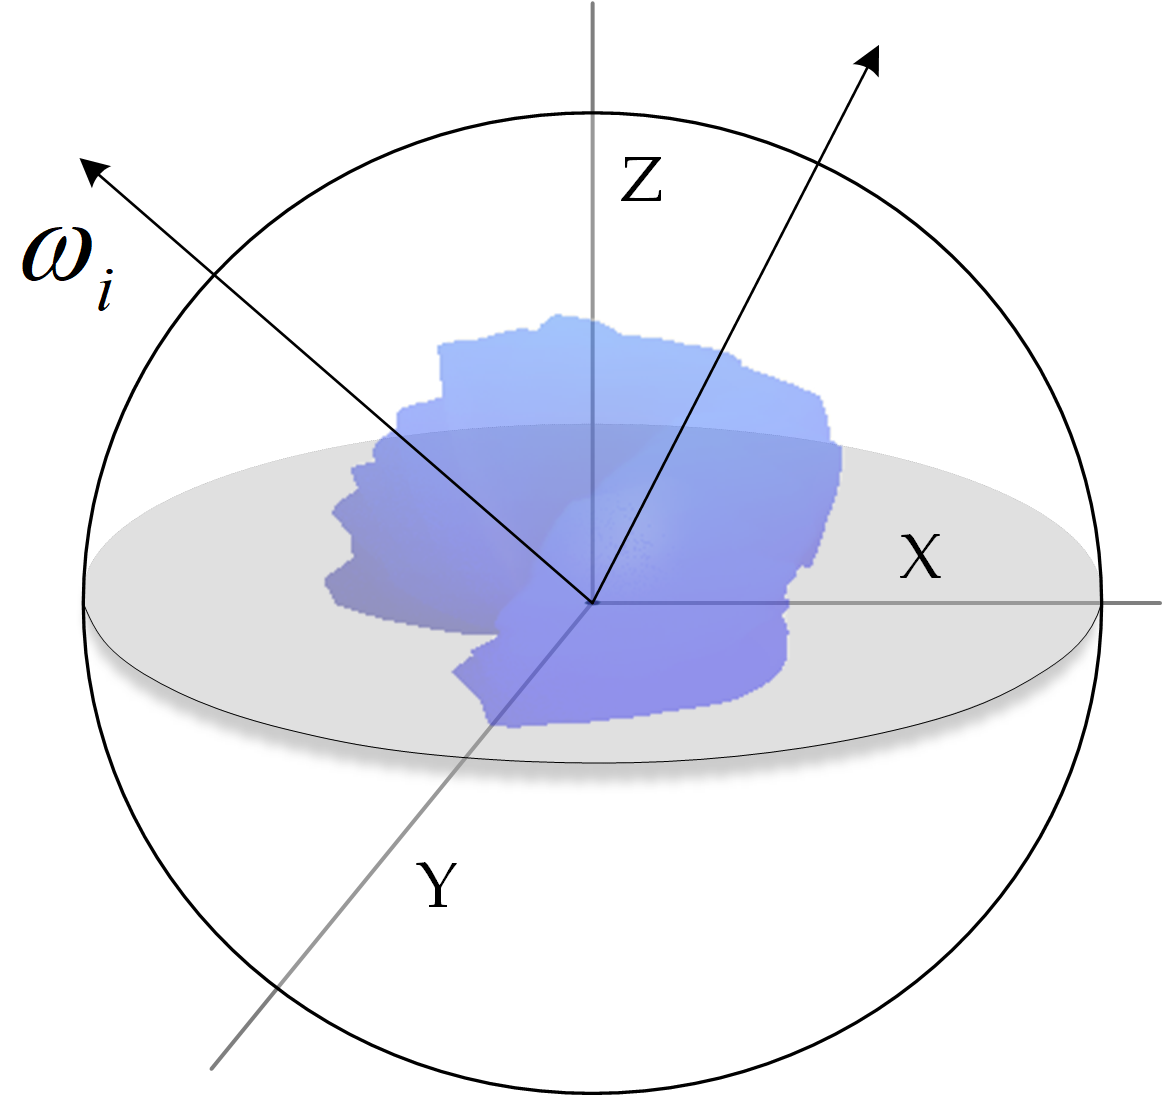
\includegraphics{figs/fundamentals/brdf_wi_wo.png}
	\caption{Parameterization of the \acrshort{brdf} response.}
	\label{fig:brdf_wi_wo}
\end{marginfigure}

In the last years, hyperspectral data acquisition has significantly increased, benefiting from the use of more cost-effective sensors and versatile platforms. On the one hand, traditional systems, which are deployed in the laboratory, are currently more efficient and capable of getting accurate spectral measurements of isotropic and anisotropic materials. These are gaining in accuracy, efficiency, and ease of use. At the laboratory level, the most accurate and well-known technique for collecting the optical features and \acrshort{brdf} of any real-world material is the use of a goniophotometer \cite{riviere_multispectral_2012}. Different variants of this configuration have been developed either to obtain better results in anisotropic materials, to take into account refraction phenomena or even to obtain normal maps, and any other characteristic that helps in synthetic modelling \cite{tunwattanapong_acquiring_2013, chen_reflectance_2014}. 

The first databases only included anisotropic materials that captured red, green and blue spectral response as a dense set of measurements \cite{matusik_data-driven_2003}, instead of analytical functions. Thus, discretized representations are more likely to be parameterized to build larger, yet realistic, \acrshort{brdf} datasets \cite{serrano_intuitive_2016}. More recently, the provided wavelengths have been extended to the whole spectra available for a motorized goniophotometer, thus allowing to extend render engines beyond the visible spectra \cite{dupuy_adaptive_2018}. As a result, \acrshort{brdf} are not solely parameterized through two spatial vectors, but also with a radiometric value. Hence, $f$ is now expressed as $f(\omega_i, \omega_o, \lambda)$, with $\lambda$ being the target wavelength. Accordingly, coarse radiometric resolution can be simulated as $\int_{\lambda_i}^{\lambda_j} f(\omega_i, \omega_o, \lambda) \hspace{1mm} d\lambda$. 

These advances lead us toward the generation of real-world material databases, which are notably used for rendering photorealistic scenes, virtual interior design in architecture, the game industry, etc. These applications can be enhanced by the increasing availability of real-world scenarios, which can be efficiently reconstructed using versatile platforms. However, building material databases is time-consuming, prohibitive when it comes to acquisition devices and requires considering a list of laboratory constraints. 

Due to the large measurement time, \acrshort{uas} flights carrying a hyperspectral sensor have been proposed for the collection of material \acrshort{brdf}. These come at expense of noisier data that must be corrected afterwards. In addition, a single or a few flights yield very incomplete spatial response due to the low variety of $\omega_o$ measurements \cite{jurado_efficient_2022}. There have been studies on atmospheric corrections for \acrshort{uas} flights, which involve correlating the at-sensor radiance to the \acrshort{hdrf} measured in the laboratory beforehand. Grayscale palettes in Lambertian materials can be used for this purpose  \cite{lucieer_hyperuasimaging_2014}. While physically-based methods have also been explored, they tend to be more time-consuming. In addition, public repositories such as the Aviris data portal (California Institute of Technology) \cite{california_institute_of_technology_aviris_nodate} offer atmospherically corrected datasets. Other widespread hyperspectral processing software, such as ENVI and Headwall SpectralView, include semi-automatic correction algorithms \cite{queally_flexbrdf_2022, jia_kernel-driven_2020, sagan_data-driven_2022}.

The lack of computational power and real-world material samples led to approximate realistic shading with analytical functions. These are easier to solve and integrate into script-based routines such as vertex and fragment shaders. They intend to emulate the appearance of real-world materials; however, continuous functions are smoothed-out versions that include errors as a consequence of fitting real data. Furthermore, fitting functions in non-linear optimizations is expensive to compute, whereas analytical functions have a low memory footprint and enable simulating a wide range of materials (with more or less precision). Hence, this \acrshort{brdf} representation was widely adopted until recently. 

\begin{marginfigure}[3cm]
	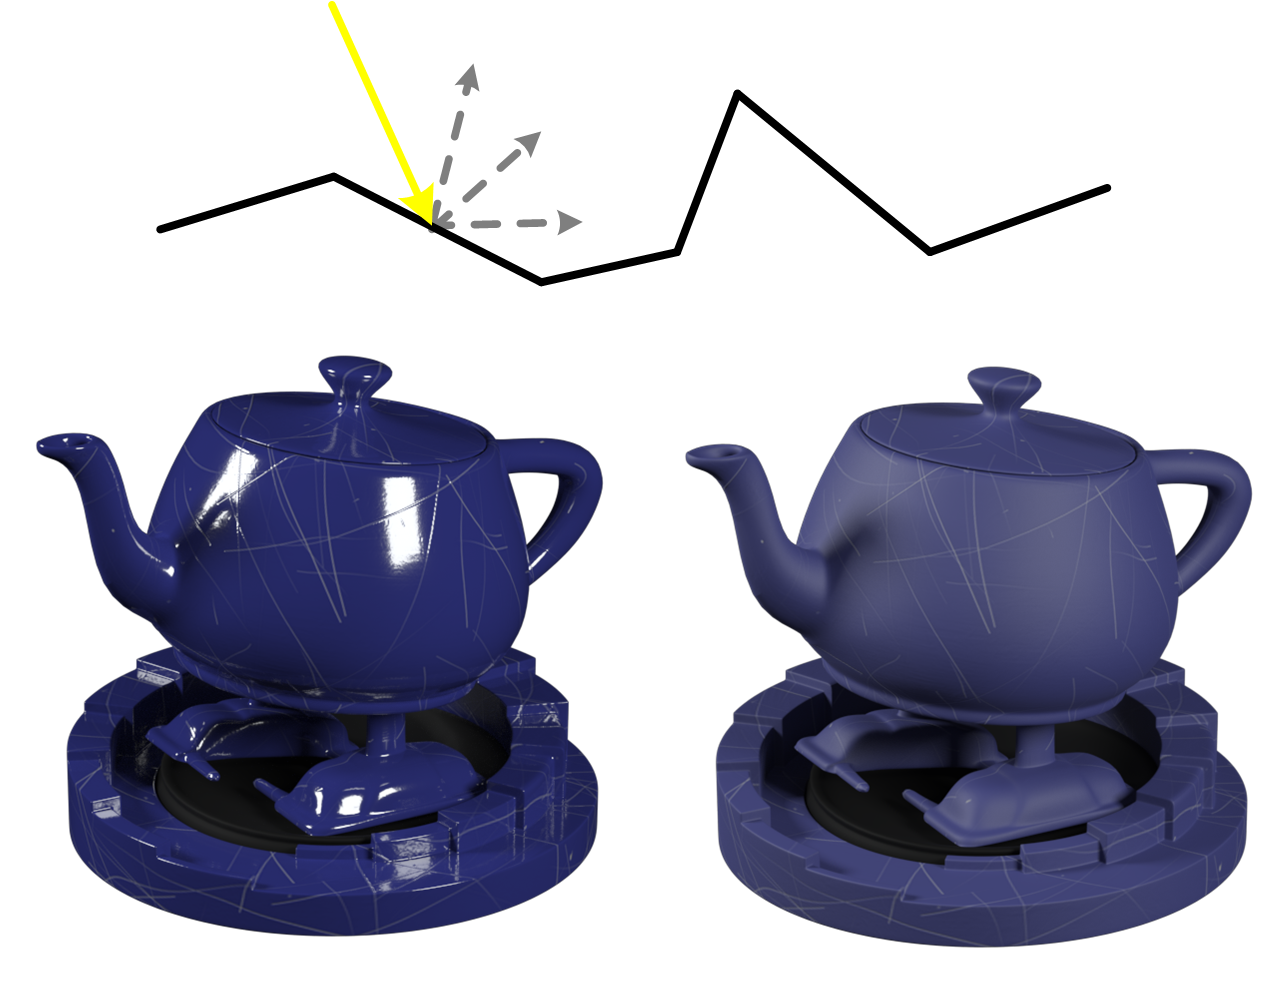
\includegraphics{figs/fundamentals/microfacets.png}
	\caption{Insight into micro facets of a surface. The striking energy reflects into the semisphere formed on the basis of the normal vector. Below, the same object is rendered as a polished and rough surface. Therefore, the second present microfacets that lead to a wider energy scattering.}
	\label{fig:microfacets}
\end{marginfigure}
Analytical \acrshort{brdf}s have a large taxonomy if we attend to the kind of material and the criteria under which these were modelled. Although most of them aim to simulate a specific appearance (metal, wood, mats, polished surfaces, the Moon, etc.), materials are at least organized into isotropic and anisotropic materials. The firsts are invariant to rotations of the surface around $n$, whereas the second changes its reflection around $n$, emulating materials such as hair or brushed metal \cite{guarnera_brdf_2016}. On the other hand, \acrshort{brdf}s are categorized as phenomenological or empirical, physically-based or theoretical and data-driven. Phenomelogical functions are computationally convenient methods for estimating the reflectance appearance of some materials, whereas theoretical make use of some attributes that intervene in physically-based shading. For instance, Phong was one of the first phenomenological models that were widely adopted with the advent of programmable pipelines. It is simply parameterized by the surface normal, $n$, the lighting vector from a single source, $l$, the view direction, $v$, and the reflection, $r$, computed according to the Fresnel law. On the other hand, Cook-Torrance is one, if not the most, representative theoretical \acrshort{brdf} as it pays attention to micro-facets, distinguished metal and dielectrics and uses the halfway vector, $h$, to compute the specular lobe. For novel \acrshort{cg} programmers, this is frequently introduced as the foundational core of Physically-Based Rendering (\acrshort{pbr}) for shader-based frameworks such as \acrshort{opengl} (Open Graphics Library). For further insight into analytical \acrshort{brdf}s, we refer the reader to the explanations of these from a theoretical point of view \cite{guarnera_brdf_2016, soldado_overview_2012}. Note that radiance spreads over a semi-sphere, and therefore, most of these functions include $\pi$ in the denominator, whereas the numerator is scaled by the $\cos$ function parameterized by $\omega_i$, $\omega_o$ and $n$. However, traditional \acrshort{cg} applications avoid downscaling the computed intensity by $\pi$ since it darkens the rendered scene and they do not intend to behave as physically-based engines. A simple demonstration of Minnaert \acrshort{brdf} is shown in Code \ref{code:analyticalbrdf}, firstly implemented to render intensity in a semi-sphere, whereas the second block is rather aimed at shading a polygonal mesh.

\vspace{3mm}

\lstinputlisting[language=c++, caption={Minnaert \acrshort{brdf} implementation for a 1) reflectance visualization tool using a semi-sphere and 2) a rendering application.}, label=code:analyticalbrdf]{code/minnaert.brdf}

\begin{figure}[ht]
	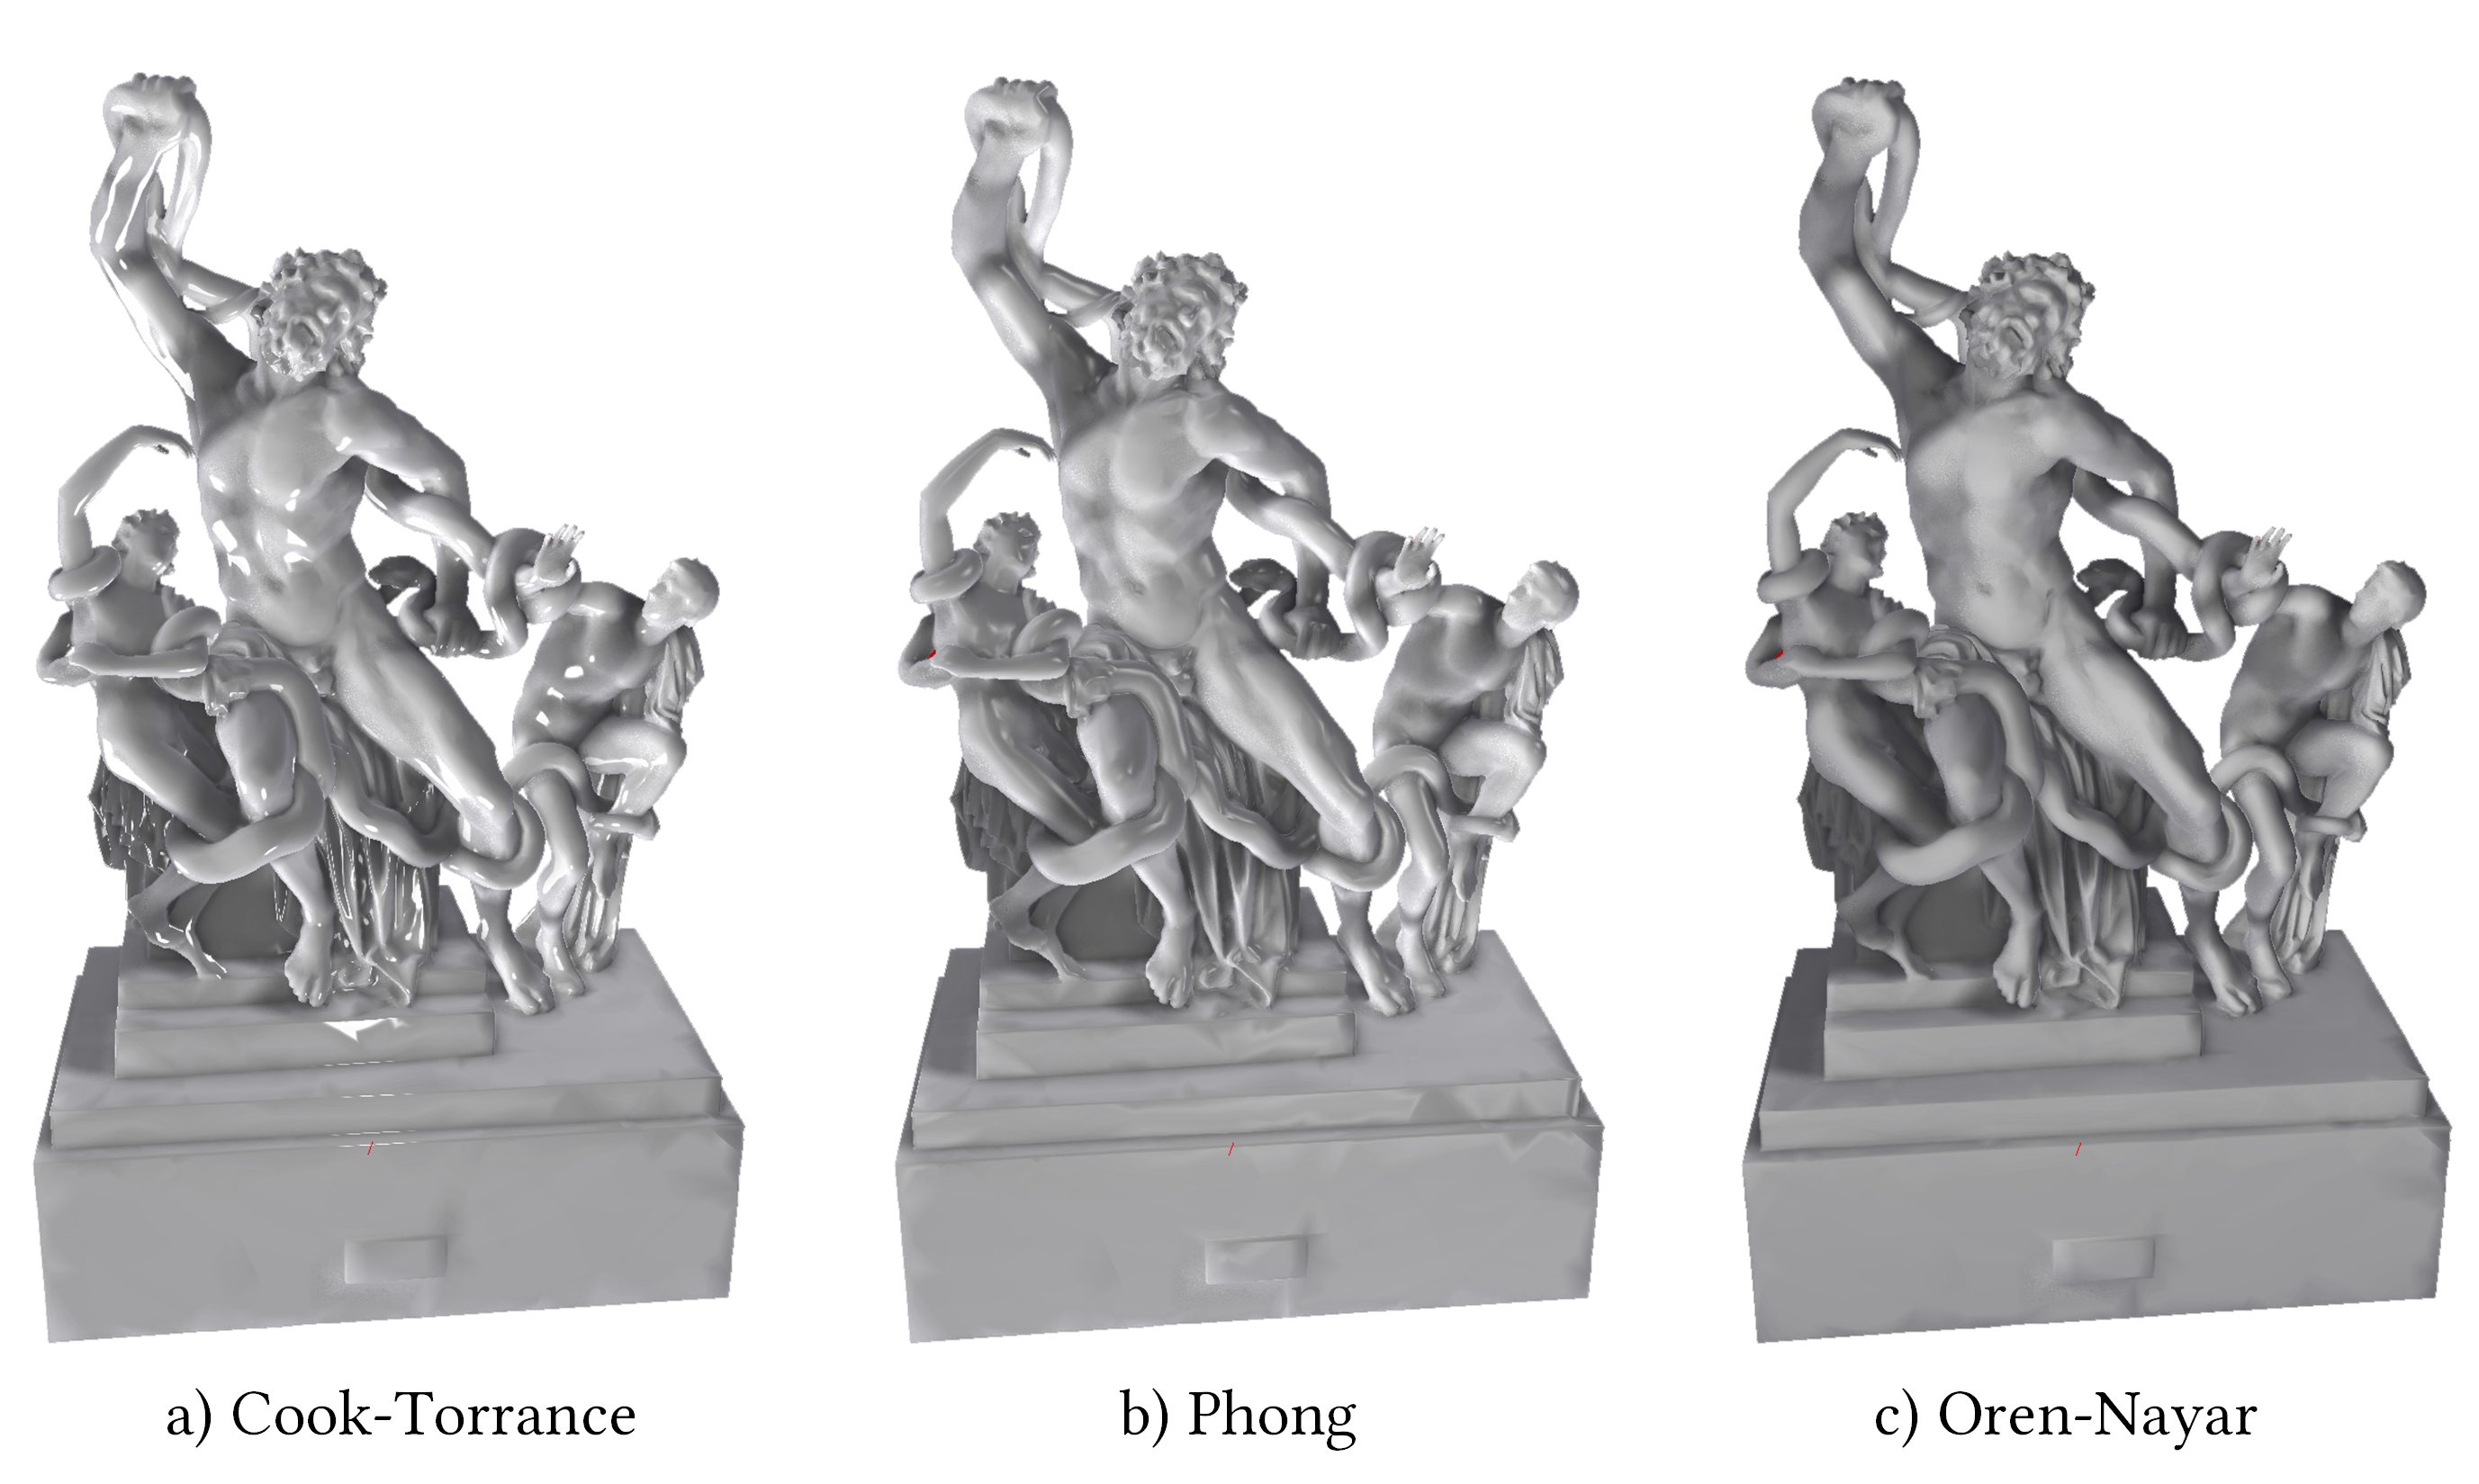
\includegraphics[width=\textwidth]{figs/fundamentals/analytical_brdf.png}
	\caption{Comparison of analytical \acrshort{brdf}s: a) Cook-Torrance ($f_0 \gets 1$, $\alpha \gets 0.077$), b) Phong ($ns \gets 32$) and c) Oren-Nayar ($\alpha \gets 0.75$). }
    \label{fig:analytical_brdf}
\end{figure}

% \begin{figure*}[ht]
%     \imageannotated{figs/fundamentals/room_rt.png}{Hello world}{0}{-2.6}{white}
% 	\caption{Comparison of analytical BRDFS: a)  }
%     \label{fig:hello}
% \end{figure*}

\section{Data types, processing and indexing}

Once the imaging devices and the interaction of light and matter have been revised, the results provided by most \acrshort{rs} tools are explained, including the main challenges that we must address if these will be the focus of our work. Then, other traditional processing algorithms which are later used are explained. These algorithms are either based on the image space or operate with 3D point clouds.

\subsection{Results from Remote Sensing}

\subsubsection{Image: vector and raster}
\label{sec:rs_data_formats}

The concept of images seems very straightforward, though the focus of this section is on the adjective preceding the image term. Besides human impression of someone or something, images are defined as "any picture, especially one formed by a mirror or a lens" by Cambridge Dictionary \cite{cambridge_english_dictionary_cambridge_2023} and "a picture of somebody/something seen in a mirror, through a camera, or on a television, computer, phone, etc." in Oxford Dictionary \cite{oxford_university_press_oxford_2023}. As a mathematical concept, an image is "a point set or set formed by mapping from another point or set", thus requiring \textbf{at least} two point sets to form an image. The subdivision of images over $\mathcal{X}$ and $\mathcal{Y}$ axes yields what is known as a pixel: the images' primitive. Despite being unique pieces of information, these are highly correlated among them and thus influenced by surrounding pixels. The significance of this conclusion is later exposed in this document to discriminate the plant variety captured in a pixel.
\marginnote[-1cm]{At least two point sets are required to form an image, though the most frequent images in the wild have three channels (visible imaging) and thus require more than two sets. For \acrshort{rs}, images with up to hundreds of channels are required for precise monitoring and data mining.}

Hence, images are discrete representations where each pixel shows the average captured radiance. However, these values are not the originally measured radiance. Instead, an Analog-to-Digital (A-to-D) conversion transforms the electrical signal into values known as Digital Numbers (\acrshort{dn}). These are typically integer values that fall in the interval $2^x$, with $x \gets 8$ being the most frequent radiometric depth \cite{navulur_multispectral_2006}, though float-point values can also be found for file formats storing uncompressed representations, e.g., \acrshort{tiff}. The radiometric resolution is especially relevant for scientific purposes where A-to-D leads to a loss of precision. Other not-that-frequent file formats store embedded \acrshort{dn}s in the image metadata, such as radiometric \acrshort{jpeg}, thus allowing us to obtain the temperature afterwards. Despite images being here referred to results acquired by sensors, the term "image" covers any pictorial representation, even generated on computers. Unlike sensing tools, computers have the advantage of working with digital data whose geometrical shapes can be defined by means of step-wise and continuous functions. As a result, the internal encoding of images does not always fits into the previous mathematical definition. The images that are not defined as a set of pixels, but rather as a set of geometrical shapes, are known as vector images instead of raster images. While vector data have no limitations on the resolution and present a lower memory footprint, raster data is easier to analyze and include in Geographic Information Systems (\acrshort{gis}) together with other layers acquired with similar spatial resolution \cite{lillesand_remote_2015}. Still, vector data is especially relevant for visualization, including \acrshort{gis} aimed at mapping Earth's cities and infrastructure (see Figure \ref{fig:raster_gis}). A comparison of raster and vector data is depicted in Figure \ref{fig:raster_vectorial}.
\begin{marginfigure}[-6.8cm]
	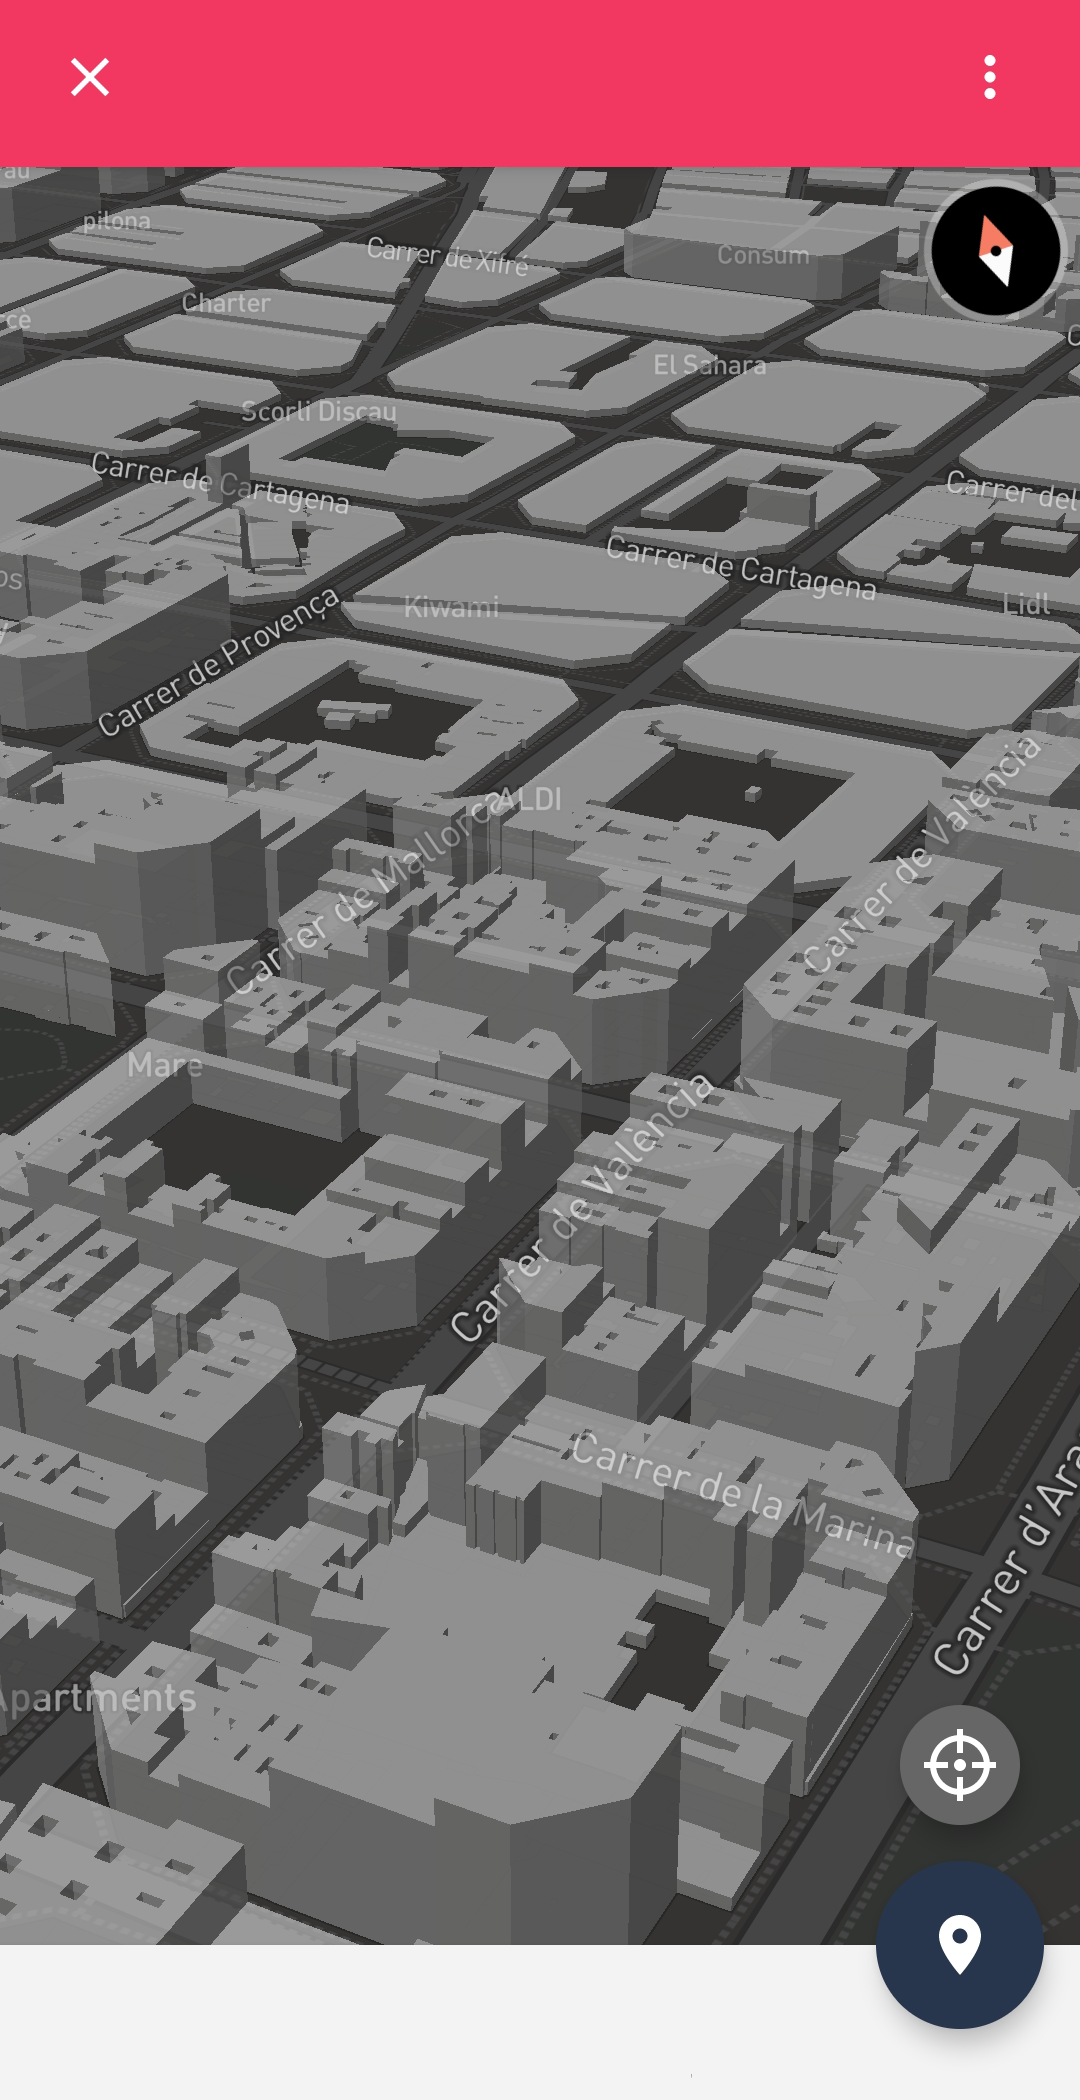
\includegraphics{figs/fundamentals/raster_gis.png}
	\caption{Vector data in a geographic information system within an Android application.}
	\label{fig:raster_gis}
\end{marginfigure}

\begin{figure}[ht]
	\includegraphics{figs/fundamentals/raster_vectorial.png}
	\caption{Comparison of a) raster and b) vector representation of Vila Real District in Portugal.  }
    \label{fig:raster_vectorial}
\end{figure}

The spatial resolution of images refers to the number of pixels represented in $\mathcal{X}$ and $\mathcal{Y}$ axes. However, it can be further stressed to introduce the amount of space in \si{\meter^2} represented in a pixel. Indeed, the latter concept is more frequent in \acrshort{rs}. It is typically derived from the image dimensions and the distance covered in $\mathcal{X}$ and $\mathcal{Y}$.

The most widespread impression of images is colour-space examples. However, there exists a considerable imagery taxonomy organized from the number of bands ($\mathcal{Z}$) and the information that is encoded in each of them. The most revised kinds of imagery are visible (colour-space), thermographic, multispectral and hyperspectral. The sensors that capture this information are coined with the same name. In this regard, Figure \ref{fig:sensor_literature} shows the percentage of research devoted to each one of the mentioned tools in the last few years. Minority tools such as \acrshort{rgb}-D, with D standing for depth, are omitted in this figure. Previous sections have delved into each one of these sensors, and their results are explained in this section. The Scopus searches were the following: $(\epsilon \cdot (\mathtt{rgb} \lor \mathtt{visible}) \lor \epsilon \cdot (\mathtt{thermal} \lor \mathtt{thermography}) \lor \epsilon \cdot \mathtt{multispectral} \lor \epsilon \cdot \mathtt{hyperspectral}) \land ((\mathtt{remote} \land \mathtt{sensing}) \lor \mathtt{uas} \lor \mathtt{uav}), \hspace{1mm} \epsilon \in \{0, 1\}$, where $\epsilon$ refers to the selection of one of the sensor keywords. 

\begin{figure}[ht]
	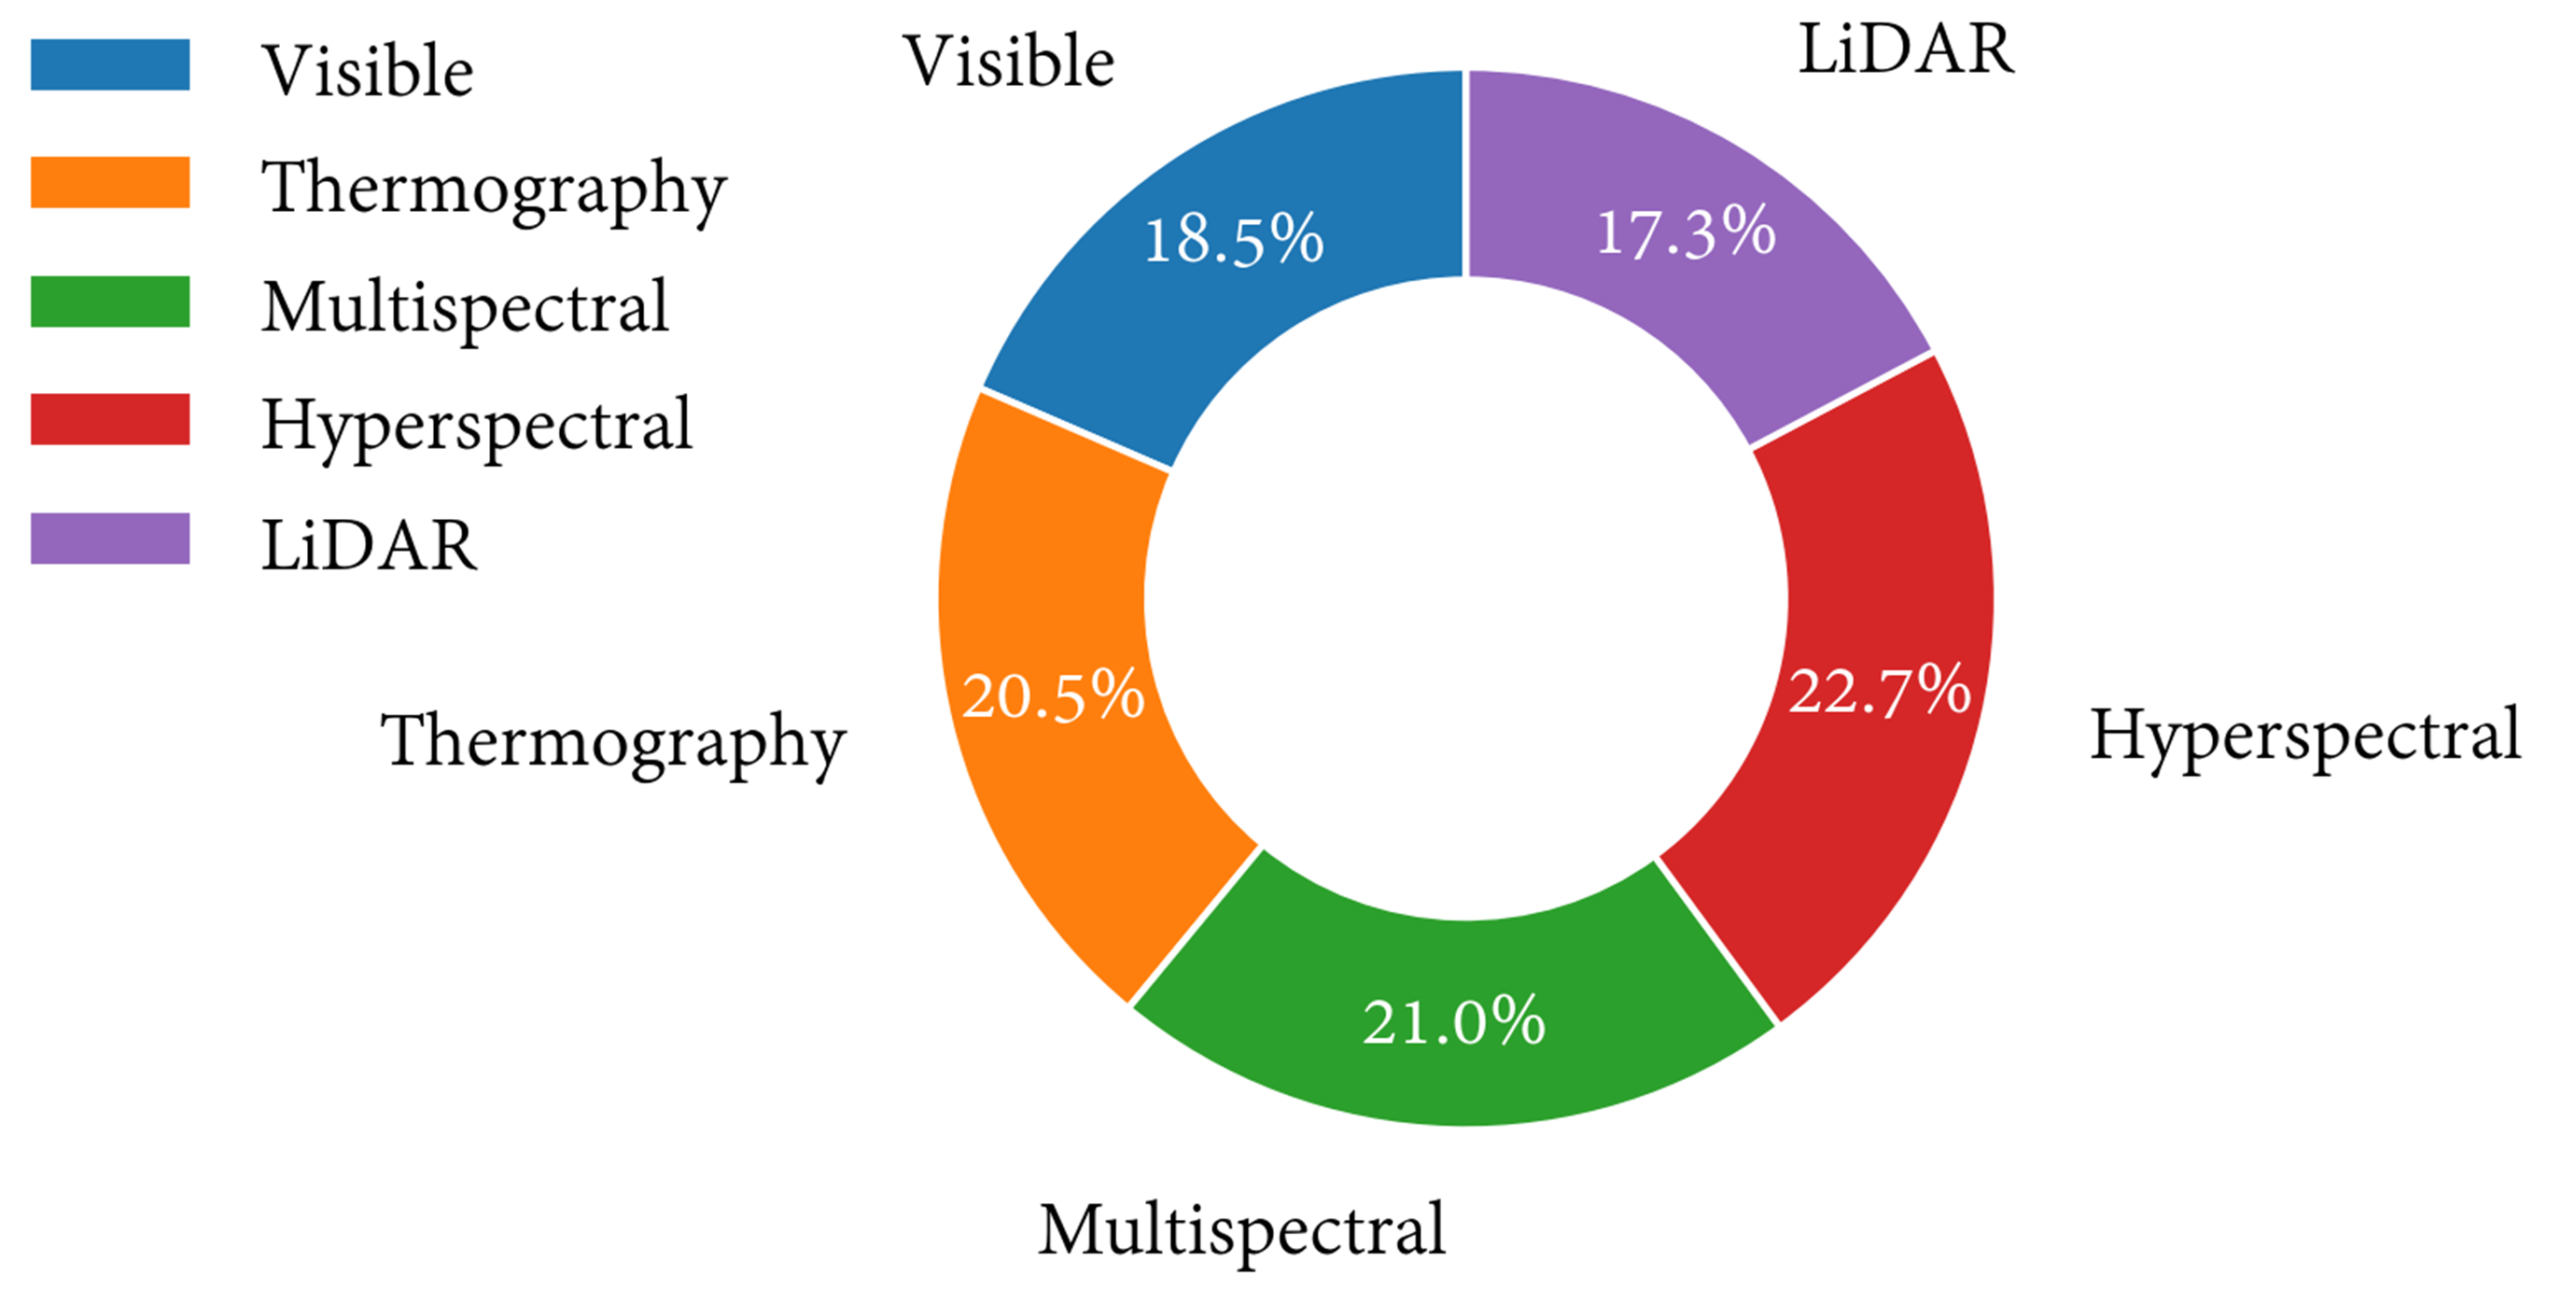
\includegraphics[width=.9\textwidth]{figs/fundamentals/literature_sensors.png}
	\caption{Number of manuscripts related to different sensors.  }
    \label{fig:sensor_literature}
\end{figure}

\subsubsection{Point clouds}

Point clouds are collections of points with no connectivity, which are typically extracted from laser scanners and photogrammetry. There exists an enormous number of hardware and software solutions measuring real-world geometry at a constant pace, including the so-called digital twins. Although images carry relevant features and lead to meaningful conclusions, these are not linked to geometry. Three-dimensional representation of real-world scenarios has enjoyed a great interest to improve visualization and interpretation of the surveyed areas and phenomena. Therefore, 3D point clouds derived from imagery can be generated, if not directly acquired with passive sensing, to facilitate the view of buildings, surfaces and any other area of interest. In contrast to 3D meshes, they enable a simpler, denser and close-to-reality representation \cite{cao_3d_2019}. Besides the positioning, points can carry further information, including colour, reflectance, intensity, normal vector and classification label, among others. Additionally, all these values can be replicated at different timestamps throughout the time scale. Reviewing the scientific literature, it can be concluded that this problem is similar to that posed in the technique called projective texture mapping \cite{debevec_efficient_1998, heckbert_survey_1986}. Initially, the aim was to have additional effects on the realistic image synthesis field of research, to cast shadows or render translucent objects \cite{dachsbacher_translucent_2003}.

The staggering pace of information acquisition and requirements concerning the level of detail of point clouds lead to massive 4D data, thus hardening the efficient storage, transmission and visualization. Yet, they are widely used in fields as disparate as autonomous driving systems, virtual and augmented reality, biomedical applications and precision agriculture. Geometric features provide further data that helps with the recognition and classification of objects, even for human operators. For instance, previous work \cite{barros_multispectral_2022, kerkech_vine_2020, de_castro_3-d_2018} have shown that elevation data significantly improves the classification accuracy on the segmentation of plots, with elevation being a derived product of photogrammetry and passive sensing. However, huge point clouds consisting of billions, even trillions of points, require up-to-date techniques that benefit from nowadays hardware, capable of massively working in parallel. The current state-of-the-art studies have extensively worked on the compression of point clouds, to save storage and reduce bit rate transmission, as well as on the efficient visualization of massive point clouds \cite{schutz_gpu-accelerated_2023, van_oosterom_organizing_2022}. 

Other operators such as the estimation of normal vectors will be following explored as it concerns a later chapter. However, this is simply a minimal part of research on point clouds, since the uncertainty from photogrammetry and laser point clouds must be individually addressed for each application. Part of this enormous amount of work comprises the classification, segmentation and identification of tree skeletons \cite{cardenas_reconstruction_2022} on point clouds. 

\subsection{Data processing}

\subsubsection{Compression}

The huge amount of point cloud data represents a challenge both for storage and transmission. Furthermore, the following massively parallel operations are performed on \acrshort{gpu} hardware with limited memory capacity. Although this drawback has been mitigated in the most recent \acrshort{gpu}s (NVIDIA GeForce 40 series at the moment this dissertation is being written), these operations ought to work over commodity hardware. The most recent releases have a memory size ranging from 8 GB (GeForce RTX 3050) to 24 GB (GeForce RTX 3090, GeForce RTX 3090 Ti \cite{nvidia_nvidia_nodate-2} and GeForce RTX 4090 \cite{nvidia_nvidia_nodate-1}), whereas laptop models have typically their memory size reduced to half of these. Other high-performance \acrshort{gpu}s focused on research, for example, NVIDIA A6000 \cite{nvidia_nvidia_nodate}, scale up to 48 GB and enable higher capacity using a bridge called NVIDIA NVLink. However, these high-performance products are not widespread, and most computers work using commodity hardware. Accordingly, GeForce Series 10 and 20 are less prohibitive, easier to acquire under stock shortage and more frequent to find in laptops not designed for high-performance tasks. The memory size of these devices is below 12 GB for Series 20 and 8 GB for Series 10. 

Furthermore, there exist frameworks for \acrshort{gpu} visualization and computing that severely clamps the maximum buffer size. For instance, \acrshort{opengl} has been the standard platform for visualization for decades. Version 4.3 introduced what is known as computer shaders, i.e., scripts solving small \acrshort{gpu} tasks that can be massively parallelized. One would expect to be able to reserve buffers with a maximum size bounded by the \acrshort{gpu}'s memory capacity; however, this limit can be queried in \acrshort{opengl}, with the \scriptsize \verb|GL_MAX_SHADER_STORAGE_BLOCK_SIZE| \normalsize keyword, returning 2,048 MB both for an NVIDIA GTX 1070 (8 GB VRAM) and an NVIDIA RTX A6000 (48 GB VRAM).

Hence, massive point clouds require at some point to be compressed, mainly in transmission and visualization applications. This research field has been coined as \acrshort{pcc}, Point Cloud Compression, distinguishing lossy and lossless methods. Similar to the computer science field, \acrshort{pcc} has transitioned from traditional techniques \cite{bui_comparative_2021}, based on encoding using data structures (regular grids, octrees, kd-trees, etc. \cite{cao_3d_2019}) to Deep Learning, where the encoding is automatically learned by convolutional autoencoders (\acrshort{cnn-ae}). The latter are more likely to lose data to some degree unless the compressed data is discrete \cite{que_voxelcontext-net_2021}, such as octree nodes. 

Very few compression methods offer low-computational complexity for real-time transmission \cite{cao_3d_2019} and reconstruction (decoding), while others do not support the compression of colour information. However, \acrshort{rs} point clouds can carry large amounts of information for every point; from \acrshort{lidar} points whose attributes follow the \acrshort{las} file standard to hyperspectral points storing spectral signatures with hundreds of measurements. Rather than exploiting the point cloud's entropy in the spatial and temporal dimensions, Graciano et al. \cite{graciano_quadstack_2021} proposed to compress layered datasets taking advantage of data redundancy. Although it was proposed to volumetric data from geology, biology or medicine fields, redundancy of sensor measurements can also be exploited for rendering. The algorithm is composed of three main steps: 1) stack redundant values on the $\textit{z}$ dimension to form the stack-based representation (\acrshort{sbr}) from the initial heightfields, 2) group stacks with the same stack content (G-stacks) and 3) organize these into a quad-tree. Spatial redundancy is not as relevant for sensor data since it captures a wide variety of materials, whereas spectral compression is feasible at expense of downscaling the radiometric resolution. 

\subsubsection{Visualization}

\begin{marginfigure}[-3.0cm]
	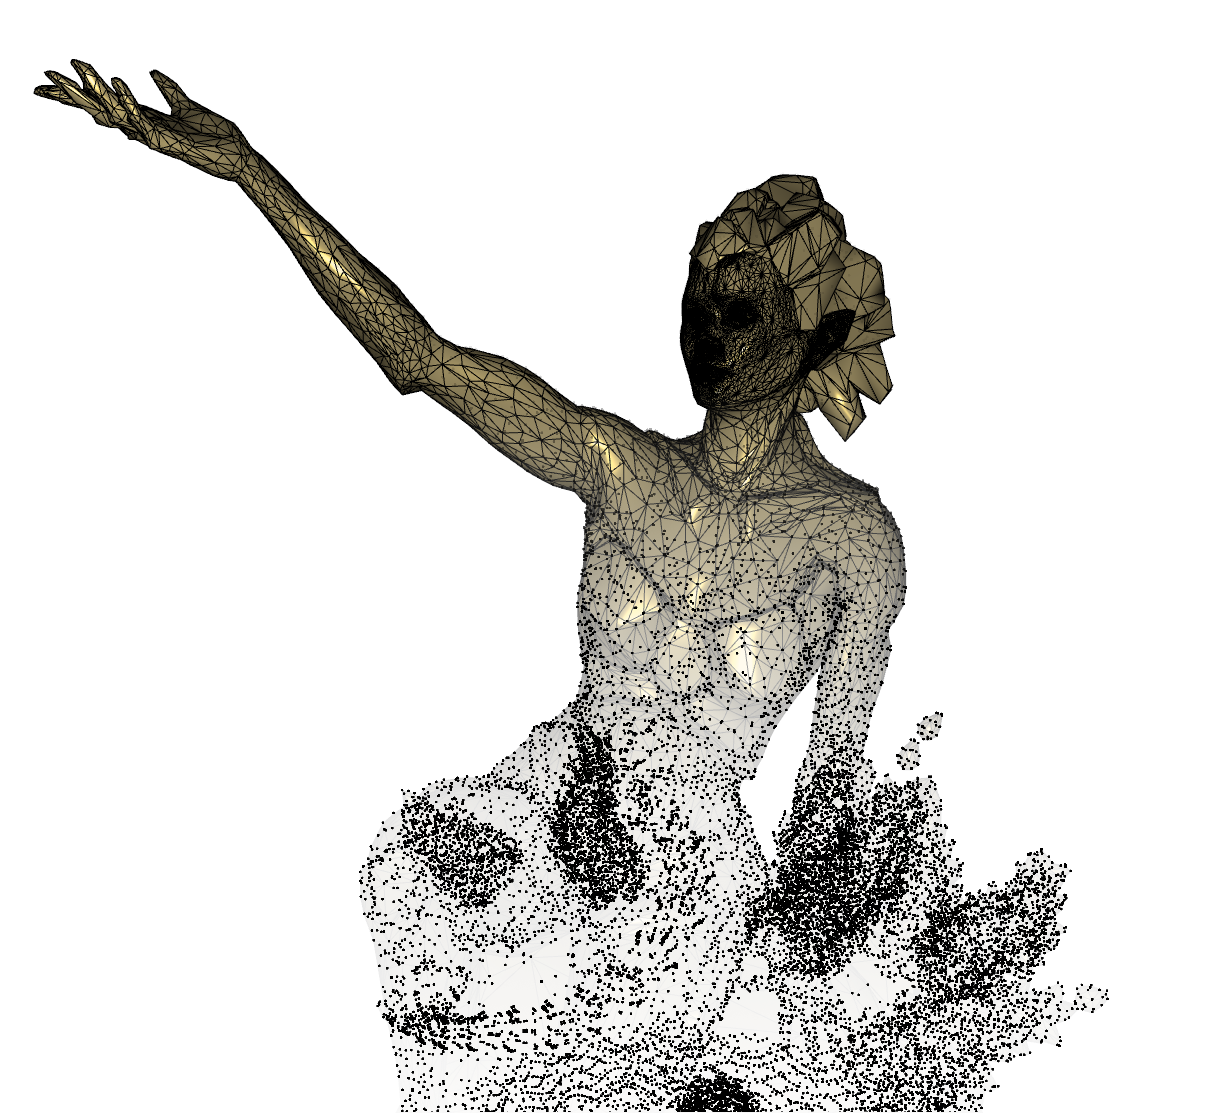
\includegraphics{figs/fundamentals/triangle_mesh_point_cloud.png}
	\caption{Transition from triangle mesh to point cloud representation, from top to bottom, with the second solely showing the triangles' vertices.}
	\label{fig:triangle_mesh_pc_comparison}
\end{marginfigure}
Unlike triangle meshes intending to emulate continuous surfaces with underlying discrete polygons, point clouds are discrete representations. Therefore, visualizing the latter is harder for scarce products with low point density (see Figure \ref{fig:triangle_mesh_pc_comparison}). This hardens the detection of features and extraction of valuable information by human operators. Computationally, it implies increasing the neighbourhood distance from which features are extracted or simply obtaining imprecise results due to the lack of data. The traditional rendering pipeline neither helps to accelerate the visualization of massive point clouds. It is designed for polygonal meshes that require 1) processing vertices, 2) including additional geometry, 3) discarding non-visible geometry, 4) rasterizing polygons, and 5) colouring polygon fragments \cite{akenine-moller_real-time_2018}.

The current state-of-the-art of massive point cloud rendering has evolved along with the impressive work of Schütz and Wimmer \cite{schutz_rendering_2019, schutz_rendering_2021}. The aim of their work was not only to speed up the visualization of billions of points but also to improve the rendered image. \acrshort{opengl}'s compute shaders were used to generate the images in the \acrshort{gpu} and recently introduced NVIDIA extensions helped to further optimize it. An alternative rendering procedure is built over \acrshort{opengl} to omit the stages 2), 3) and 4) of the traditional pipeline. In this work, vertices were massively projected into an image that is later rendered as a texture. However, the order in which points were projected showed to have a big impact on the performance. Points were transformed into Morton codes of 30 bits, 10 for every dimension, and sorted according to them. Then, globally sorted points were shuffled into small batch groups, whose size is determined by Graphic Processing Clusters (\acrshort{gpc}s). Rather than distributing the work linearly, the \acrshort{gpu} organizes it into 2D patches assigned to \acrshort{gpc}s. Thus, global sorting helps in grouping framebuffer updates, but it is suboptimal due to workload unbalancing. Spatially close \acrshort{gpc}s in charge of visible points at a timestamp $t$ are assigned a heavy workload, while others remain idle. The random shuffling of globally sorted points using small batches was proved to slightly enhance the rendering performance.

\begin{figure}[ht]
	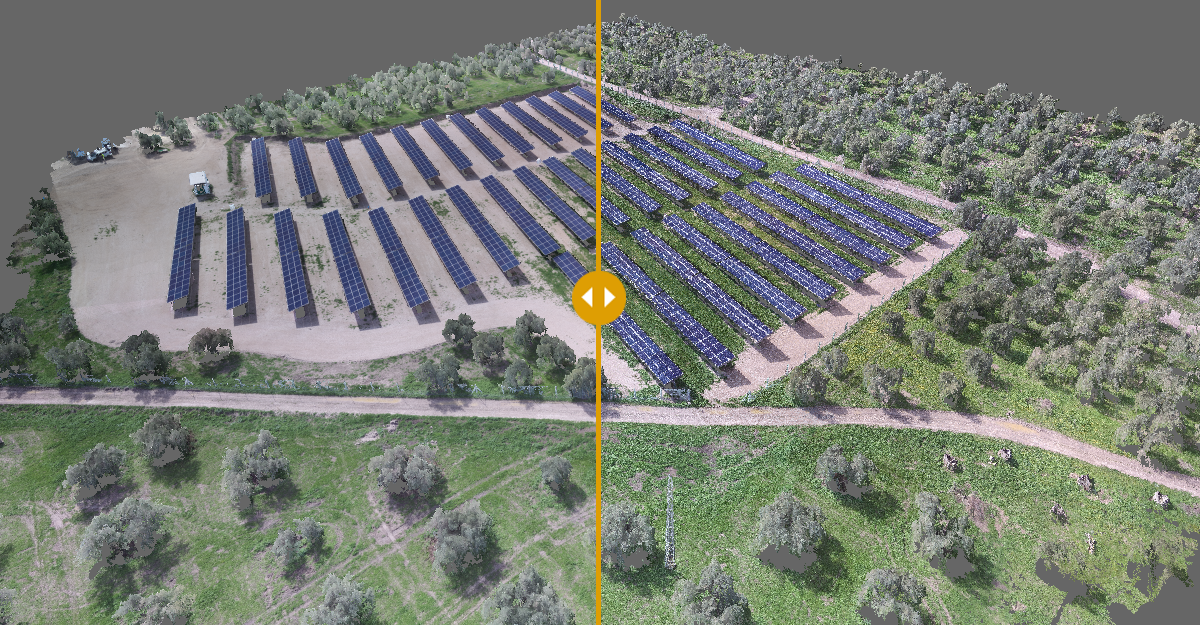
\includegraphics[width=\textwidth]{figs/fundamentals/hqs_comparison.png}
	\caption{On the left part, colouring using a mixed representation of surrounding points and on the right side, using a sole point colour for each pixel. This image was obtained using the procedure described by Schütz and Wimmer \cite{schutz_rendering_2021}. }
    \label{fig:hqs_pc_rendering}
\end{figure}

\begin{kaobox}[frametitle=Compute shader core proposed by Schütz and Wimmer]
The projection approach from Schütz and Wimmer \cite{schutz_rendering_2021} uses modern \acrshort{opengl} extensions following this pipeline:
\begin{itemize}
    \item The depth buffer is firstly computed, with the depth being encoded along with the point index (64 bits). The atomic minimum operators help to select the point with the minimum depth. However, this approach leads to a noisy-like rendering for sparse point clouds. Instead, the depth of a pixel takes into account several points; data is exchanged within thread groups whose points fall in the same pixel using \verb|shuffleNV| and \verb|ballotThreadNV| operators. Then, \verb|shuffleXorNV| computes the minimum depth within a pixel neighbourhood.
    \item Colours are iteratively accumulated: the limited capacity of SSBOs may require that multiple point cloud subdivisions aggregate data. Accumulations can be implemented using atomic operators, whereas (red, green) and (blue, alpha ($\alpha$)) channels are encoded in two different buffers with values of 64 bits. Hence, the alpha channel is also used for accounting for the number of visible points at each pixel.
    \item Aggregated colours are finally transformed by averaging the mean value for each channel. Pixels with $\alpha \gets 0$ are coloured with the background tone. 
\end{itemize}
\end{kaobox}

Lately, optimizations of point cloud renderings have focused on the \acrshort{lod} and organization into Layered Point Clouds (\acrshort{lpc}). A key in the construction of these data structures is that they ought to be view-dependent to enable adjusting the \acrshort{lod} based on the camera position and direction. \cite{schutz_gpu-accelerated_2023} proposed to index point clouds with octrees whose inner nodes are voxelized, whereas leaf nodes lead to the point primitives. Ogayar et al. \cite{ogayar-anguita_nested_2023} managed to create an adaptive hierarchical structure that coupled different data structures at different levels. It was shown to retrieve larger amounts of points with higher average and peak throughput. Previously, Schütz et al. \cite{schutz_software_2022} sorted points with their Morton codes, split them into batches and built a hierarchical data structure using these batches as leaf nodes. Visualization of \acrshort{lod}s varies according to the camera, and therefore, patches of different point densities could be rendered for distant objects. If the underlying discrete levels of a \acrshort{lod}-based data structure are visible, they are referred to as rendering artefacts. Van Oosterom et al. \cite{van_oosterom_organizing_2022} proposed to organize point clouds into a Space Filling Curve (\acrshort{sfc}) and compute the continuous \acrshort{lod} of every point, thus enabling gradual changes in the point density. 

Noise in point cloud visualization was also mitigated by Schütz et al. \cite{schutz_rendering_2019, schutz_rendering_2021} using modern \acrshort{opengl} extensions. Individual \acrshort{gpu} threads are grouped in subgroups, also known as warps, of size 32 in NVIDIA microarchitectures, that can communicate efficiently and exchange results. For a globally sorted point cloud, warps work over spatially close points that can aggregate colour data. Hence, this approach leads to a High-Quality Shading (\acrshort{hqs}) variant \cite{schutz_rendering_2021} that provides a more continuous shading (see Figure \ref{fig:hqs_pc_rendering}). This also opens the possibility of filling holes derived from lower point density rather than reconstruction failures. 

\subsubsection{Occlusion detection}

The projection of additional sources of information over point clouds is trivial once camera poses are estimated. For each viewpoint, the camera matrix enables the projection of 3D points into the image plane. However, projections do not separate background and foreground surfaces; although a point may be theoretically visible from a camera, it could be covered by another surface in the real scenario. The chances are that points are visible in more than a single viewpoint, and therefore, erroneous assignments of information may be partially masked by other correct measurements. However, this approach is not precise for colouring point clouds and occlusion must be detected to tackle this.    

\begin{marginfigure}[1cm]
	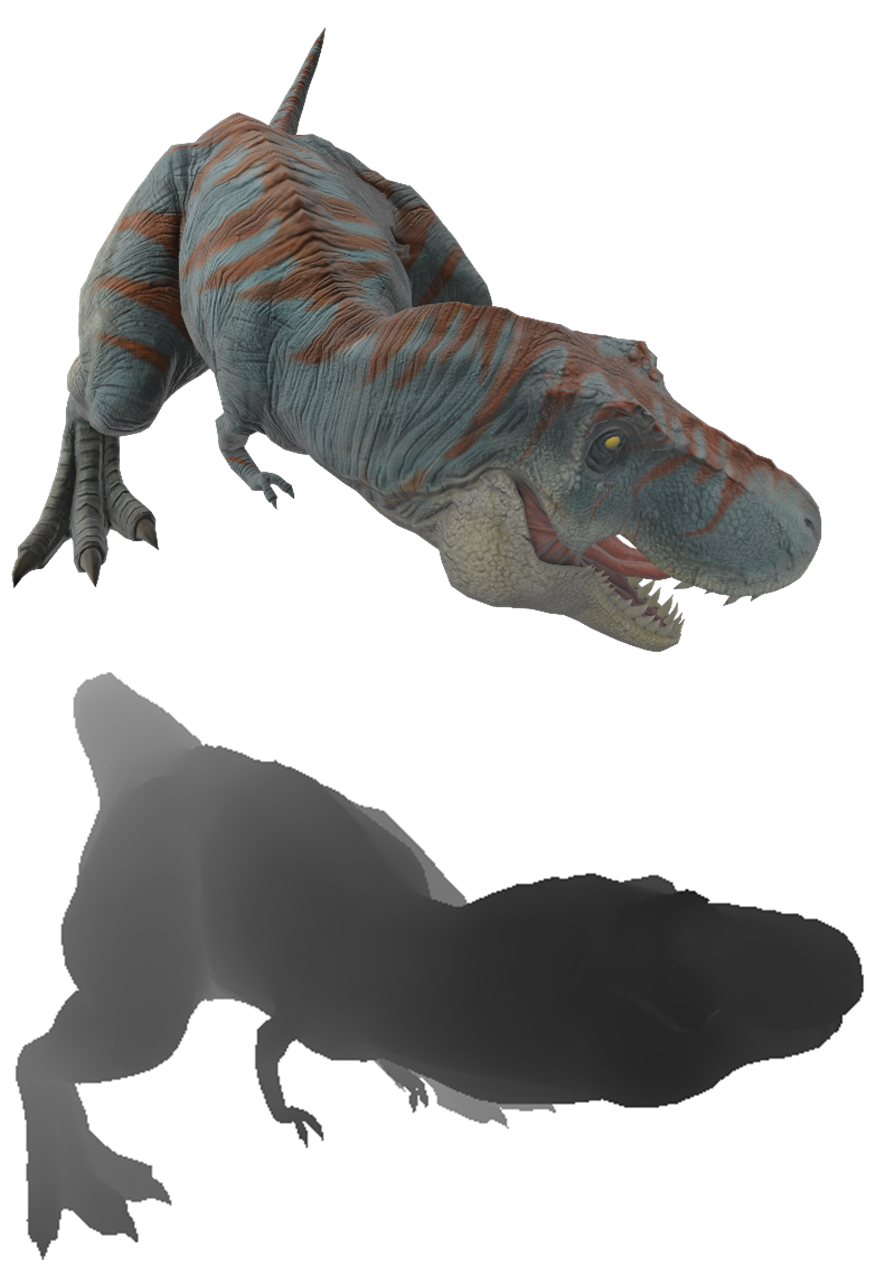
\includegraphics{figs/fundamentals/z-buffer.png}
	\caption{Shading of a 3D model along with the depth captured in a $z$-buffer.}
	\label{fig:z-buffer_opengl}
\end{marginfigure}
The most straightforward way to detect occlusion is to use what is called $z$-buffers in rendering: images that store for each pixel the minimum depth at which geometry was projected. It has been traditionally used for shadowing and discarding non-visible geometry for optimizing the rendering \cite{akenine-moller_real-time_2018, white_cascaded_2021}. Similarly, it enables recording the nearest visible point at every image's pixel. It does not require indexing points into a data structure, though they are of great help to narrow the subset of points to be projected into a single viewpoint. Determining the nearest depth is trivial in the \acrshort{gpu}, as most \acrshort{gpgpu} frameworks provide atomic operations. Despite these being supposedly slower operations, they compete well against other approaches in terms of memory consumption and efficiency. Jurado et al. \cite{jurado_out--core_2022} proposed to build out-of-core occlusion-aware multispectral point clouds in Compute Unified Device Architecture (\acrshort{cuda}). Asynchronous data loading and computation were applied to complete $z$-buffers for hundreds of images and point clouds of up to 1,084M points. Instead of using $z$-buffers, Jo et al. \cite{jo_dense_2021} computed the point and camera distance to solely project information from the closest viewpoint. This approach leads to errors if the point remains occluded from the closest one, though it can work over very dense and uniform image datasets. Not to mention this colour assignment is more prone to noise, while aggregations mitigate it. 

\begin{figure}[ht]
	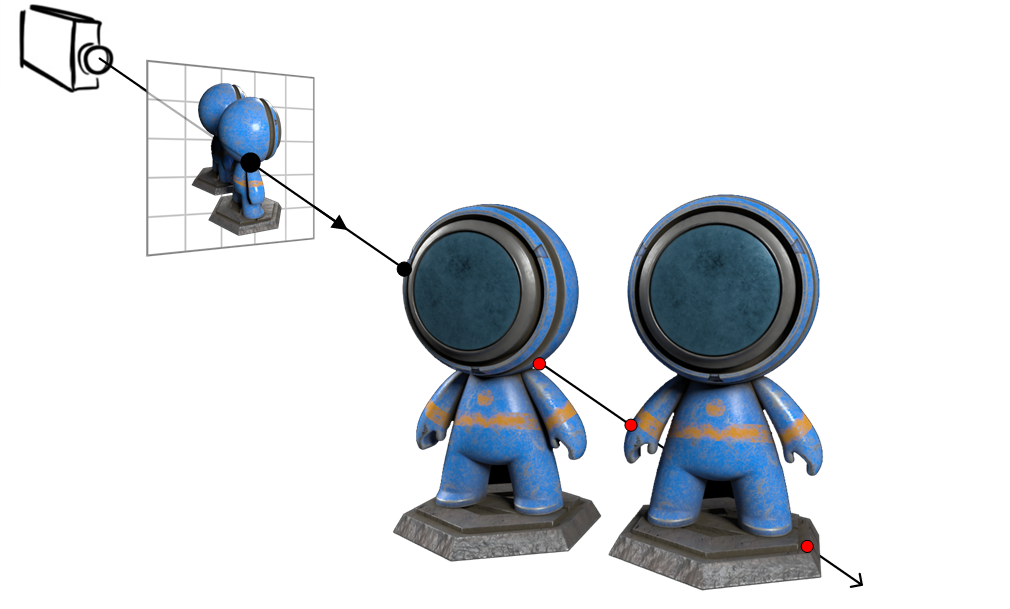
\includegraphics[width=\textwidth]{figs/fundamentals/occlusion.png}
	\caption{Occlusion of left figure over the right one on a projection made from the left part of the scene. }
    \label{fig:occlusion_concept}
\end{figure}

An alternative to $z$-buffers is to estimate the underlying polygon mesh of point clouds. In this regard, occlusion can be detected by constructing a small triangle mesh from points surrounding the main one \cite{jurado_multispectral_2020}. The point neighbourhood was sought using $k$-nearest neighbours (\acrshort{knn}). Although this method may achieve good results over planar surfaces, polygonal meshes are harder to reconstruct in other scenarios, for example, forestry with dense and incomplete vegetation. Other studies benefit from additional sources of information to detect occlusion, such as the semantic segmentation of point clouds \cite{schneider_fusing_2010}. 

\subsubsection{Photogrammetry}

\begin{marginfigure}[2.0cm]
	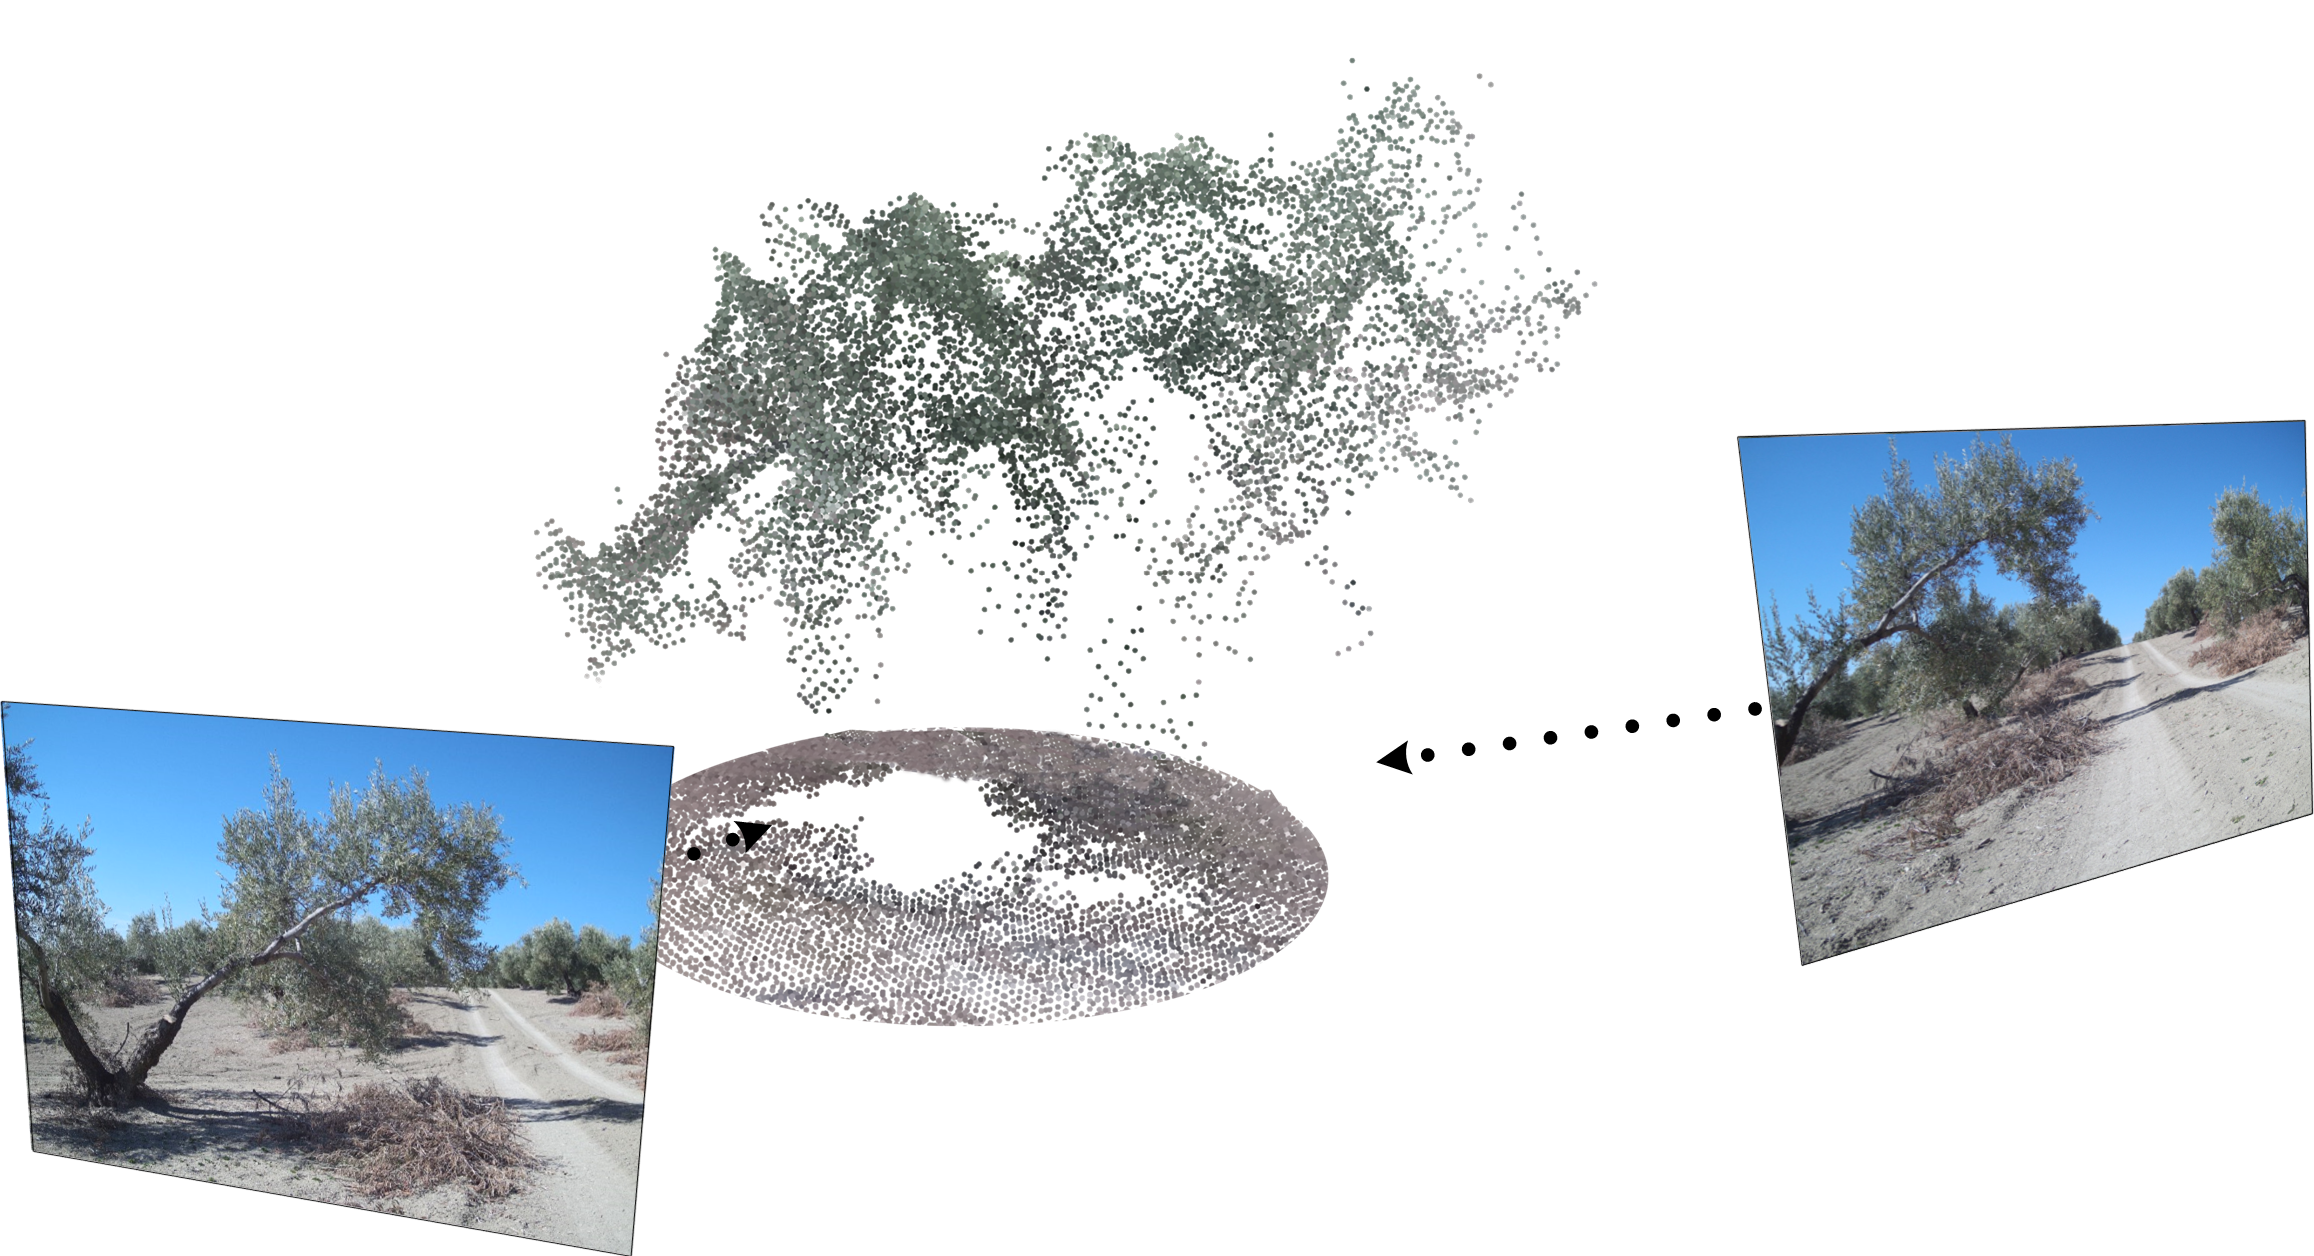
\includegraphics{figs/fundamentals/terrestrial_photogrammetry.png}
	\caption{Finding of keypoints visible in two images acquired from ground, which lead to estimating the camera pose and generating a 3D point cloud.}
	\label{fig:terrestrial_photogrammetry}
\end{marginfigure}
Photogrammetry refers to the science and technology of generating geometrically correct products derived from photographs. 3D reconstructions are fundamental in this dissertation, as they provide an automatic procedure for modelling scenes, in contrast to Computer-Aided Design (\acrshort{cad}) tools, arm-mounted probes and active methods. However, mapping is also derived from what was coined as photogrammetry: the fusion of image datasets to compound results that helps in the understanding and visualization of target areas. Some of the most common maps are Digital Surface Models (\acrshort{dsm}), Digital Terrain Models (\acrshort{dtm}) and orthophotos. These products are estimated from datasets ranging from terrestrial (Figure \ref{fig:terrestrial_photogrammetry}) and \acrshort{uas}-based imagery, which is known to be acquired sequentially in most cases, and large datasets from publicly available data. The latter images are harder to manipulate since one of their major stems is crowd-sourcing from the Internet: data published by users with very different devices, lighting conditions, visible objects in the scene, etc.

The transition from laboratory to outdoor was possible due to the advent of digital images with higher resolution, better computational capabilities and mature techniques. The overall procedure in photogrammetry is 1) to estimate parameters from cameras, 2) to reconstruct 3D points and 3) to reconstruct materials if necessary. Two slightly different techniques have had great success in recent years: Structure from Motion (\acrshort{sfm}) and Visual Simultaneous Localization and Mapping (\acrshort{vslam}), though this section is focused on the first. 

The \acrshort{sfm} method comprises a vast literature, but it has been robustly applied for over 20 years. The basis consists of 1) detecting key points in images, 2) matching these key points among multiple images, 3) estimating camera parameters from previous links and 4) building \acrshort{sfm} models. The final step, despite not being part of \acrshort{sfm}, is to reduce errors from estimations, also known as bundle adjustment (\acrshort{ba}). The error to be minimized is formally defined as follows (Equation \ref{eq:error_bundle_adjustment}) \cite{furukawa_multi-view_2015}:
\begin{gather}
    \label{eq:error_bundle_adjustment}
    \begin{aligned}
        E(P, M) = \sum_{j} \sum_{i \in V(j)} \mid P_i(M^j) - m_{i}^{j} \mid^2
    \end{aligned}
\end{gather}
where P is a set of camera parameters, ${P_i}$, $M^j$ represents a set of 3D coordinates of a track, $m_{i}^{j}$ are the projections of $M^j$ in the i-th camera, $V(j)$ are the list of caneras where point $M^j$ is visible and $P_i(M^j)$ is the projection obtained by using the camera parameters $P_i$.

SfM is also found in the literature as \acrshort{sfm}-\acrshort{mvs}, with \acrshort{mvs} referring to Multi-View Stereo. \acrshort{mvs} originated as an improvement to two-view stereo algorithms. Instead, thousands of images are applied to the reconstruction of large metropolitan and natural scenes. However, the main concerns in this regard are the photo consistency of features that are identified in several images. As we previously stated, conditions may vary from one viewpoint to another; hence, it is required to calculate how likely a candidate in $V_i$ is the correct match of a pixel in $V_j$, with $i \neq j$. Finding candidates for every feature over huge datasets is neither trivial nor efficient. Therefore, most of nowadays photogrammetric software is programmed in the \acrshort{gpu} to accelerate the pipeline.

Applying photogrammetry is not prohibitive, and it is even possible to find mobile-based applications that can work over cost- and time-efficient imagery recorded on mobile phones. Computer-based solutions, aimed at large datasets, include open-source and commercial software. The first group includes ColMap, AliceVision, Zephyr and VisualSfM, whereas notable commercial software includes Pix4DMapper \cite{zheng_thermal_2020}, Agisoft Metashape \cite{grechi_3d_2021}, RealityCapture and Autodesk Recap 360 \cite{lafi_3d_2017}. The first two commercial solutions are sped-up using multi-core \acrshort{cpu} and \acrshort{gpu} acceleration for image matching, whereas \acrshort{ba} is performed in the \acrshort{cpu}. \cite{jiang_efficient_2020} revised the efficiency of \acrshort{sfm} implementations by applying it over four datasets. According to their evaluation, performed using commodity hardware, Metashape showed the worst performance both for \acrshort{ba} and feature matching, whereas RealityCapture showed similar performance during feature matching and significantly better during \acrshort{ba}. However, Agisoft Metashape generated the densest point clouds for every dataset. Also, reported results in the literature depend on the computer used during the experiments and yet, they may vary over a short period of time. For example, Agisoft Metashape is currently known to support accelerated processing in the GPU for image-matching, depth-map reconstruction and other mesh-related operations. It works over \acrshort{cuda}-enabled \acrshort{gpu}s, and therefore, it was not expected to provide results as discouraging as reported by \cite{jiang_efficient_2020}.

\subsubsection{Colour aggregation}

A final remark must be done on colour aggregations. Points receive multiple values that may vary one from another since these are captured under different lighting and viewing conditions. The observed radiance varies according to the viewing angle, expressed through azimuth, $\phi \in [0, 360]$, and zenith, $\delta \in [0, 180]$, angles. Also, surfaces behave so that the emitted radiation is not spread uniformly unless it is a perfect Lambertian generator \cite{vollmer_infrared_2017}. Surfaces emit more radiation if $\delta = 0$, i.e., the camera's view vector is $-\hat{n}$, the normal vector of the surface. The naïve and widespread way to solve aggregations is to average them \cite{javadnejad_photogrammetric_2020, hoegner_3d_2016}, while consensual approaches minimize the distance from the aggregated value to the originals. The latter method has been mainly applied to expert-guided decision-making to aggregate opinions following those operators that minimize the conflict among the experts' views.

Instead of averaging samples, multiple aggregation functions can be used together with penalty functions to select that provides the result which differs less from the experts' opinions. In this context, experts are different camera viewing angles obtaining distinct results. The use of penalty functions is on computing the similarity of each aggregation and the starting samples \cite{bustince_definition_2017, bustince_penalty_2017}, which must be maximized. Although penalty functions have been gaining interest in scientific research, they have barely been explored in some contexts such as image processing \cite{paternain_color_2012}. 

\begin{figure}[ht]
	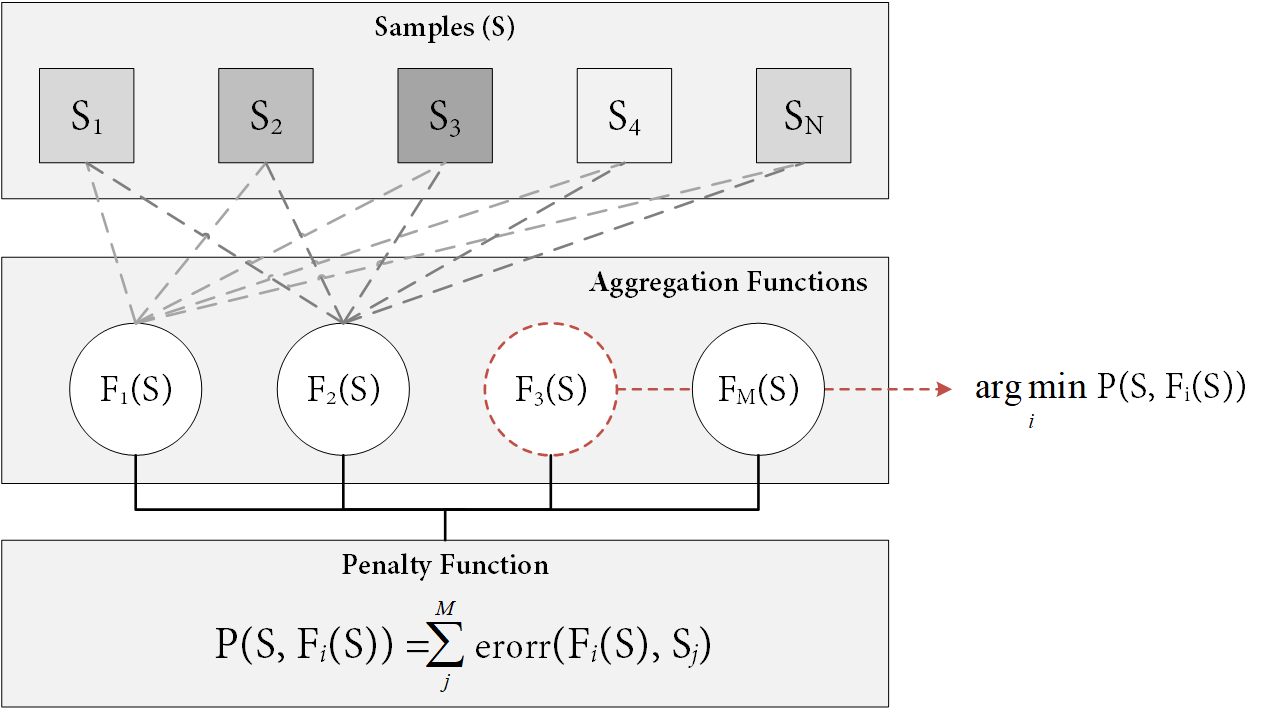
\includegraphics[width=\linewidth]{figs/fundamentals/penalty_functions.png}
	\caption{Overall procedure to compute the penalty value of every available aggregation.}
	\label{fig:penalty_funtions}
\end{figure}
Briefly, n-ary aggregation functions, $f: [0, 1]^n \rightarrow [0, 1]$ are monotone increasing and satisfy the boundary conditions (Equation \ref{eq:aggregation_boundary1}).  
\begin{gather}
    \begin{aligned}
        &\forall i \in \{1,...,n\}, \hspace{1mm} x_i \leq y\\
        &\Rightarrow f(x_1,...,x_n) \leq f(x_1,..., x_{i-1}, y, x_{i+1},...,x_n)\\
        &f(x_{\textit{min}},...,x_{\textit{min}}) = x_{\textit{min}}\\
        &f(x_{\textit{max}},...,x_{\textit{max}}) = x_{\textit{max}}
    \end{aligned}
    \label{eq:aggregation_boundary1}
\end{gather}

On the other hand, averaging aggregation functions are bounded by the minimum and maximum input (Equation \ref{eq:aggregation_boundary2}).
\begin{gather}
    \label{eq:aggregation_boundary2}
    \begin{aligned}
        \min{\{x_1,...,x_n\}} \leq f(x_1,...,x_n) \leq \max{\{x_1,...,x_n\}}
    \end{aligned}
\end{gather}

Finally, penalty functions, $P: \R^{2} \rightarrow \R$, satisfy the conditions in Equation \ref{eq:penalty_conditions}, where \textit{y} is the aggregated value. Consequently, penalty functions can be expressed as $\sum_{i=1}^{n} P(x_i, y)$ with the goal of retrieving the aggregation that minimizes the value of $P$, $g(x) \gets \operatorname*{argmin}_y P(x, y)$.
\begin{gather}
    \label{eq:penalty_conditions}
    \begin{aligned}
        &P(x_i,y) = 0 \hspace{2mm} \forall x_i = y\\
        &P(x_i,y) > 0 \hspace{2mm} \forall x_i \neq y\\
        &P(x_i,y) \ge P(x_j,y), \hspace{1mm}\mid x_i - y \mid > \mid x_j - y \mid\\
    \end{aligned}
\end{gather}

\subsubsection{Normal estimation}

Point clouds, either derived from photogrammetry or passive sensing, lack certainty in most of the attributes that provide further value to this product, ranging from normal vectors to semantic labels of different levels of detail. Many studies work on solving the uncertainty of these attributes, where normal estimation is a recurrent topic. This operation is provided as a ready-to-use tool in some widespread libraries for point cloud processing, for example, \acrshort{pcl} (Point Cloud Library) and \acrshort{cgal} (Computational Geometry Algorithms Library). Since these are very time-consuming tasks, implementations are even facilitated as multi-core solutions that significantly reduce the latency. 

Most methods addressing normal estimation operate over neighbourhoods of varying dimensionality that correlate points to form minimal triangle meshes, from which normal vectors are estimated. Thus, the main challenges in this procedure are selecting an appropriate neighbourhood size and noise resilience, as these factors greatly contribute to wrong estimations. From the neighbourhood, plane fitting is approached using unweighted Principal Component Analysis (\acrshort{pca}) and Singular Value Decomposition (\acrshort{svd}). Another challenge is the efficiency of the method: seeking the nearest $n$ points is not trivial nor efficient unless memory-consumpting data structures are built into point clouds. Hence, some works have proposed to perform a global sort on the basis of Morton codes calculated from $\textit{xyz}$ coordinates \cite{jakob_optimizing_2021}. This way, the neighbourhood is narrowed to spatially close indices on a linear buffer.

With current trends in \acrshort{ai}, normal estimation has also been achieved with Deep Learning techniques. It can be achieved by representing point clouds as graphs \cite{lenssen_deep_2020} and images \cite{zeng_deep_2019, boulch_deep_2016} since it must be performed per point rather than per voxel. To this end, additional sources of information such as depth and Hough transform \cite{boulch_deep_2016} help with the normal estimation along with $\textit{xyz}$ coordinates. 

\subsubsection{Parallel processing}

This section is focused on the revision of approaches for parallelizing processes concerning \acrshort{rs}, rather than on specific applications. The key term in this brief section is GPGPU, General-Purpose computing on Graphics Processing Units, which is a programming field that takes advantage of GPUs to rapidly solve parallelizable tasks. This is possible due to the large number of cores this hardware comprises. 

In this regard, \acrshort{opengl} is the most widespread solution since it allows both rendering and solving computing tasks using massive geometry. From a rendering approach, point clouds have their own primitive in the draw calls, \verb|GL_POINTS|. It follows the standard rasterization pipeline while processing point clouds for rendering, despite some of these are not required for such a primitive. This drawback can be sorted out with other already explained approaches implementing a custom pipeline \cite{schutz_rendering_2021, schutz_software_2022}. For problems involving parallel computing and rendering, \acrshort{opengl} is an easy-to-use platform as it allows developers to resolve both tasks at once. However, one of the main shortcomings of \acrshort{gpgpu} \acrshort{opengl} is the handling of asynchronous tasks that could overlap to get the most out of the \acrshort{gpu}'s capabilities, which is very limited in \acrshort{opengl} and constrained to the use of barriers. More recently, \acrshort{opengl} has been discontinued at expense of more efficient and adaptive graphics frameworks such as Vulkan, which are expected to turn into the standard frameworks in this field. Since these are still ongoing and remain niche, very few works use these platforms \cite{stumpfegger_gpu_2022}.  

Another standard framework for GPGPU is \acrshort{cuda}. As opposed to \acrshort{opengl}, it is not a cross-platform tool; instead, it is only able to operate over NVIDIA GPUs, but it also provides a more flexible GPGPU framework. With \acrshort{opengl} being discontinued, most GPGPU studies that used \acrshort{opengl} has transitioned to \acrshort{cuda} over time \cite{schutz_gpu-accelerated_2023}. Nevertheless, recent NVIDIA extensions have been introduced on both platforms. Other \acrshort{gpu}-based rendering and computing platforms are DirectX \cite{baek_accelerated_2020} (Windows OS), OpenCL (cross-platform) and Metal for Apple platforms.

\subsection{Data indexing}

This subsection introduces the reader to a shallow notion of efficient data structures for indexing point clouds and triangle meshes. This is not part of the state-of-the-art of this dissertation; instead, the aim is to understand the data structures that will be following mentioned.

This work is intended to provide scalable yet efficient products to fuse data sources and emulate them. Therefore, data structures used in ray tracing, one of nowadays most challenging \acrshort{cg} fields, are a good fit for our later implementations. Ray-tracing is mainly intended for physically-based simulations of energy spreading, with applications ranging from realistic rendering (Figure \ref{fig:ray_tracing_room}) to \acrshort{lidar} simulations and non-line-of-sight rendering aimed at finding hidden geometry \cite{royo_non-line--sight_2022}. In spite of the wide range of applications, geometry indexing in ray tracing has been mainly narrowed to Boundary Volume Hierarchies (\acrshort{bvh}) \cite{meister_survey_2021} (Figure \ref{fig:bvh_raytracing}). It is a binary tree that helps to rapidly discard parts of the scene during the traversal (half of the remaining scene with each new traversal step). Building a \acrshort{bvh} is immediate, though doing it efficiently and making later queries efficient is not as trivial. The way primitives are merged, whether a bottom-up approach is considered, has a significant impact on the traversal. The quality of a \acrshort{bvh}, once built, is measured through a cost function that estimates the minimum number of operations to find the nearest primitive. The probability of interior nodes is typically estimated with the Surface Area Heuristic (\acrshort{sah}) shown in Equation \ref{eq:sah}, which correlates the geometry of an interior node and its parent node. 
\marginnote[1cm]{
    \begin{equation}
        P(N_c|N)^{\textit{SAH}} = \frac{\textit{SA}(P(N_c))}{\textit{SA}(P(N))}
        \label{eq:sah}
    \end{equation}
}
\begin{marginfigure}[-5.0cm]
    \includegraphics{figs/fundamentals/room_rt.png}
	\caption{Ray-tracing rendering of a 3D modelled room. }
    \label{fig:ray_tracing_room}
\end{marginfigure}

\begin{figure}[ht]
	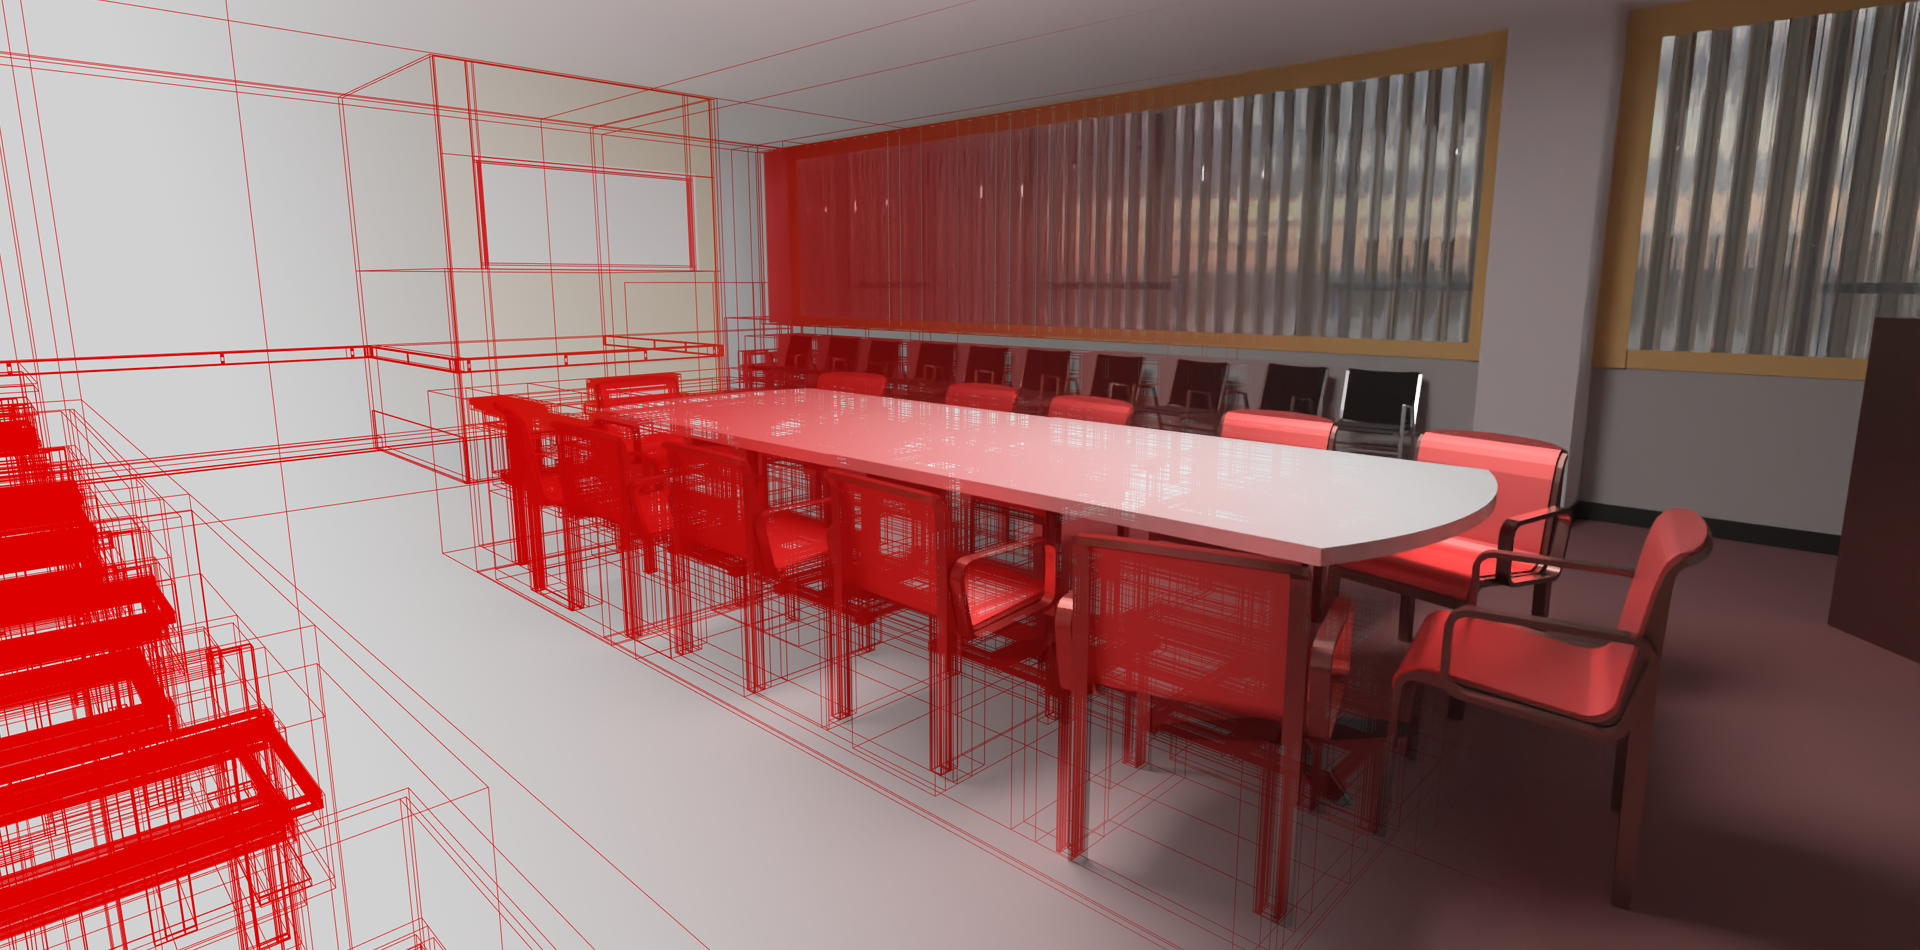
\includegraphics[width=\textwidth]{figs/fundamentals/bvh_raytracing.png}
	\caption{Rendering of the BVH data structure (left side) for indexing the traditional Conference room \cite{mcguire_computer_2017} on the right side. }
    \label{fig:bvh_raytracing}
\end{figure}

BVHs can either be constructed with bottom-up, top-bottom and incremental approaches. The quality of a BVH cannot be estimated until completion; therefore, the merging/splitting operations are guided by heuristics. From now on, this section will be mainly explained using the algorithm of Meister and Bittner \cite{meister_parallel_2018}, which is the bottom-up construction followed in this work. The aforementioned heuristics, for instance, can be guided by the area of the bounding box enclosing two nodes for a bottom-up approach. The tighter the bounding box, the better is for later traversals. Note that larger boxes intersect a larger number of rays, thus increasing significantly the number of tests. Sometimes, however, larger boxes are intentionally preferred to avoid primitive intersection tests which are harder to resolve than ray-box collisions.

A significant challenge is to efficiently determine which are the surroundings of a primitive. It has been typically approached using what is known as Morton codes (or $Z$-curve), a data representation that encodes $x$, $y$ and $z$ coordinates with $\lfloor{\frac{2^r}{3}\rfloor}$ bits. $r \gets 5$ with 10-bit representations are the most frequent, though it can be increased to $r \gets 6$ for a higher \acrshort{lod}. This data encoding happens to sort $xyz$ points in 3D following a curve that goes through $X$, $Y$ and $Z$ axes. Therefore, a 1D buffer of Morton codes can be sorted to rapidly determine which are the neighbours of a primitive using a radius $R$. It may not return the optimal neighbour primitive for creating a new node, though it is much more efficient. Yet, $R$ can be increased at expense of higher response time whether a better \acrshort{bvh} quality is required (if the heuristic is good enough). 

Another shortcoming is to incorporate massive parallelism in the \acrshort{gpu}. The algorithm of Meister and Bittner \cite{meister_parallel_2018} is guided by heuristics and shortcuts in spatial searches, and yet, highly detailed scenes are composed of millions of triangles (e.g., a power plant of $\sim$13M triangles has been traditionally used for comparisons \cite{mcguire_computer_2017}). However, binary-tree inspired algorithms are not a \textit{rara avis} in the \acrshort{gpu}; indeed, they are very frequently used to cope with simultaneous readings and writings in non-overlapping indices with a complexity of $\mathcal{O}(n\textit{log}(n))$. For instance, the partial summation up to each index was coined as \textit{prefix-sum} or \textit{prefix-scan}, which can be resolved in the \acrshort{gpu} with up-sweep (reduce) and down-sweep phases \cite{nguyen_gpu_2007}. Similarly, \acrshort{bvh} construction can follow a merge and compact approach where the nearest neighbour is sought, these nodes are merged and then they are compacted in a global buffer. The \textit{prefix scan} algorithm enables the later compaction since it counts how many nodes are prior to any new node, thus determining its location in the global buffer.

One would expect the later traversals to be easier than the initial construction. Nonetheless, the first shortcoming is the looping and stack-based traversal; the first makes threads stall until the traversal is terminated, whereas the latter requires storing local access data for every thread. These shortcomings are even harder when the ray-tracing engine does not solely requires the first hit, but also any hit. Stackless traversals have been proposed, but most of them still have a memory footprint despite being lower \cite{meister_survey_2021}. It is caused by traversals requiring at least some kind of binary encoding of the path. Once footprint and traversal drawbacks are overcome, or at least mitigated to some degree, ray traversals can be further optimized by grouping rays which may have a similar outcome \cite{hendrich_ray_2019}. In this work, we approached ray traversals in \acrshort{bvh}s using a stack with local data. For millions of rays, the \acrshort{gpu} will stall for seconds as this procedure is neither efficient nor have a low memory footprint, though it is solved in much less time than would require in the \acrshort{cpu}. 

\begin{marginfigure}[0.0cm]
    \includegraphics{figs/fundamentals/bvh_clustering.png}
	\caption{Node clustering at different BVH levels. }
    \label{fig:bvh_clustering}
\end{marginfigure}
Finally, there are other data structures beyond the \acrshort{bvh} which are not as fast for ray traversals. Among them, regular grids, kd-trees and octrees are the most widespread. The first is very fast to construct ($\mathcal{O}(1)$ insertions), although it is not adaptive and queries may lead to performing a large number of ray-polygon intersection tests. It also has a great memory consumption whether a higher \acrshort{lod} is required to lower the number of intersection tests. On the other hand, octrees and kd-trees are adaptive and thus have a lower memory footprint. Subdivisions in octrees are equal splits of a bounding box, whereas kd-trees partitioning relies on the sorting of primitives along $X$, $Y$ and $Z$ axes. Hence, the former is slightly more efficient on the construction ($\mathcal{O}(\log{n})$, in contrast to the $\mathcal{O}(kn \log{n})$). Ray traversals have been long studied for octrees \cite{revelles_efficient_2000}, kd-trees \cite{dos_santos_kd-tree_2009} and regular grids \cite{amanatides_fast_1987} and do not represent a challenge; however, \acrshort{bvh}'s bounding boxes are tighter, i.e., the bounding box of the parent node is not split among its internal nodes (see Figure \ref{fig:bvh_clustering} and \ref{fig:data_structures_indexing}). The latter approach favours that fewer ray-box intersection tests are positive. Note that all these data structures can be constructed so that parallelism is maximized in multi-core environments, as regarded by Karras \cite{karras_maximizing_2012}.

\begin{figure*}[ht]
	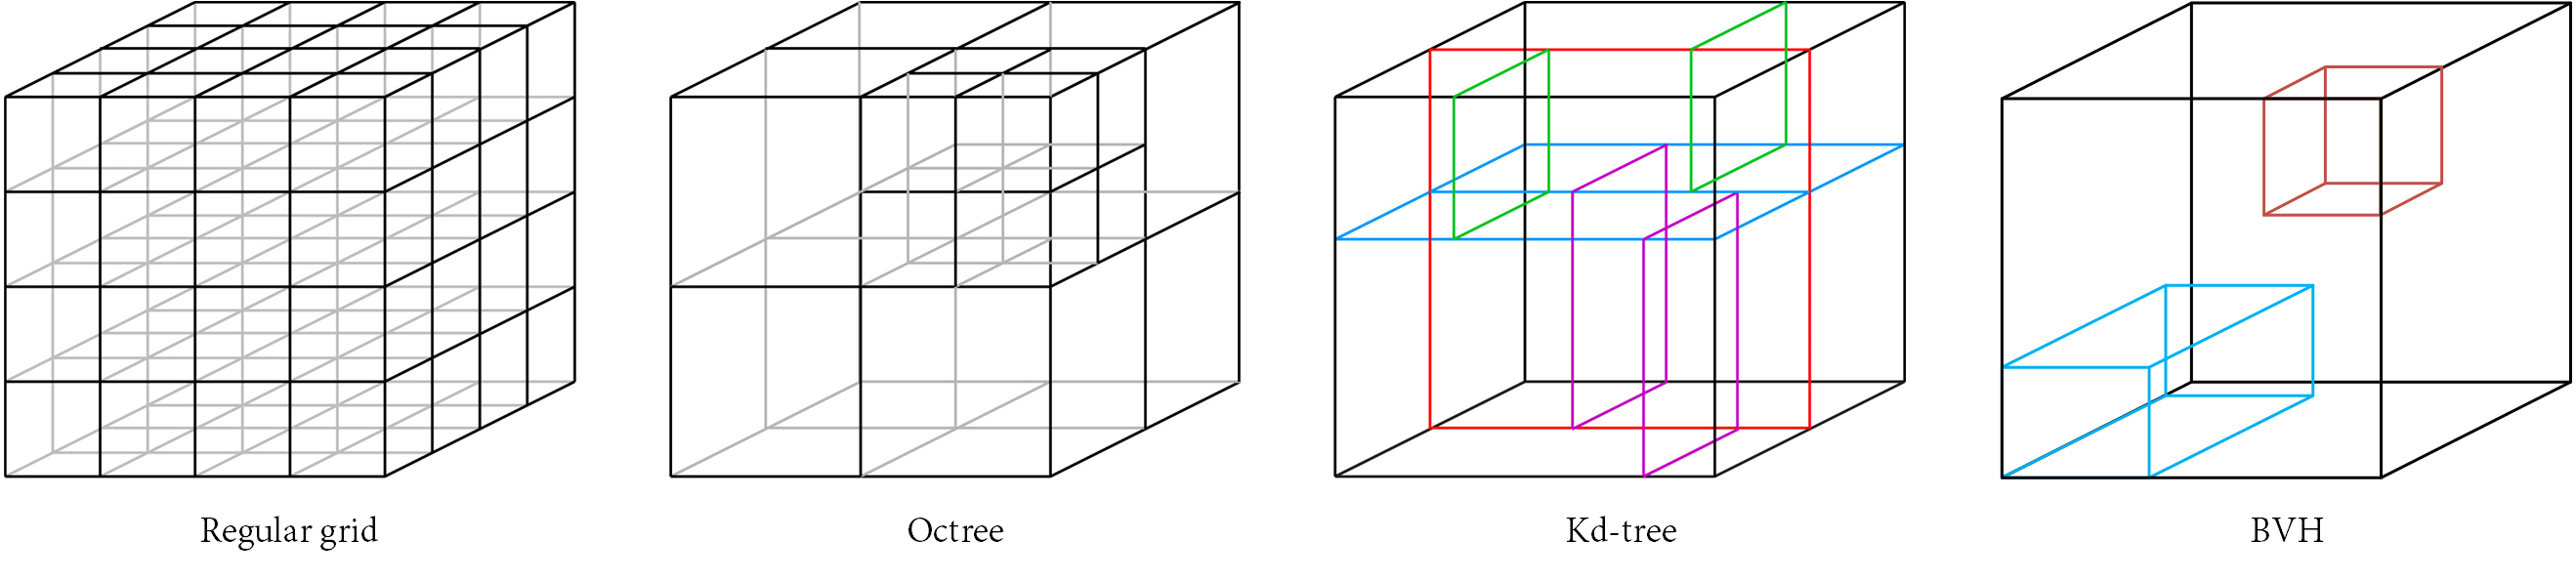
\includegraphics[width=\linewidth]{figs/fundamentals/data_structures.png}
	\caption{From left to right: regular grid, octree, kd-tree and BVH. Part of the image was obtained from Ogayar et al. \cite{ogayar-anguita_nested_2023}. }
    \label{fig:data_structures_indexing}
\end{figure*}
%\setchapterpreamble[u]{\margintoc}
\chapter{Simulation, fusion and analysis of sensor data}
\labch{context}
\label{sec:context_rs}

The previous chapter presented the fundamentals of Remote Sensing which are required for this dissertation, including the notion of images, point clouds and widespread active and passive sensing tools. Different products are the result of these sensors, whereas data ought to be kept in a compact way for subsequent analyses. Hence, pixels from 2D maps, or points from 3D point clouds, are required to have a stack-based representation from each one of the available images. Figure \ref{fig:available_spectra} summarizes which parts of the spectra are available and which sensors provide this kind of information. Based on previous fundamental concepts, the state-of-the-art concerning the fusion of heterogeneous data, simulation and analysis are following presented.

\begin{figure}[ht]
	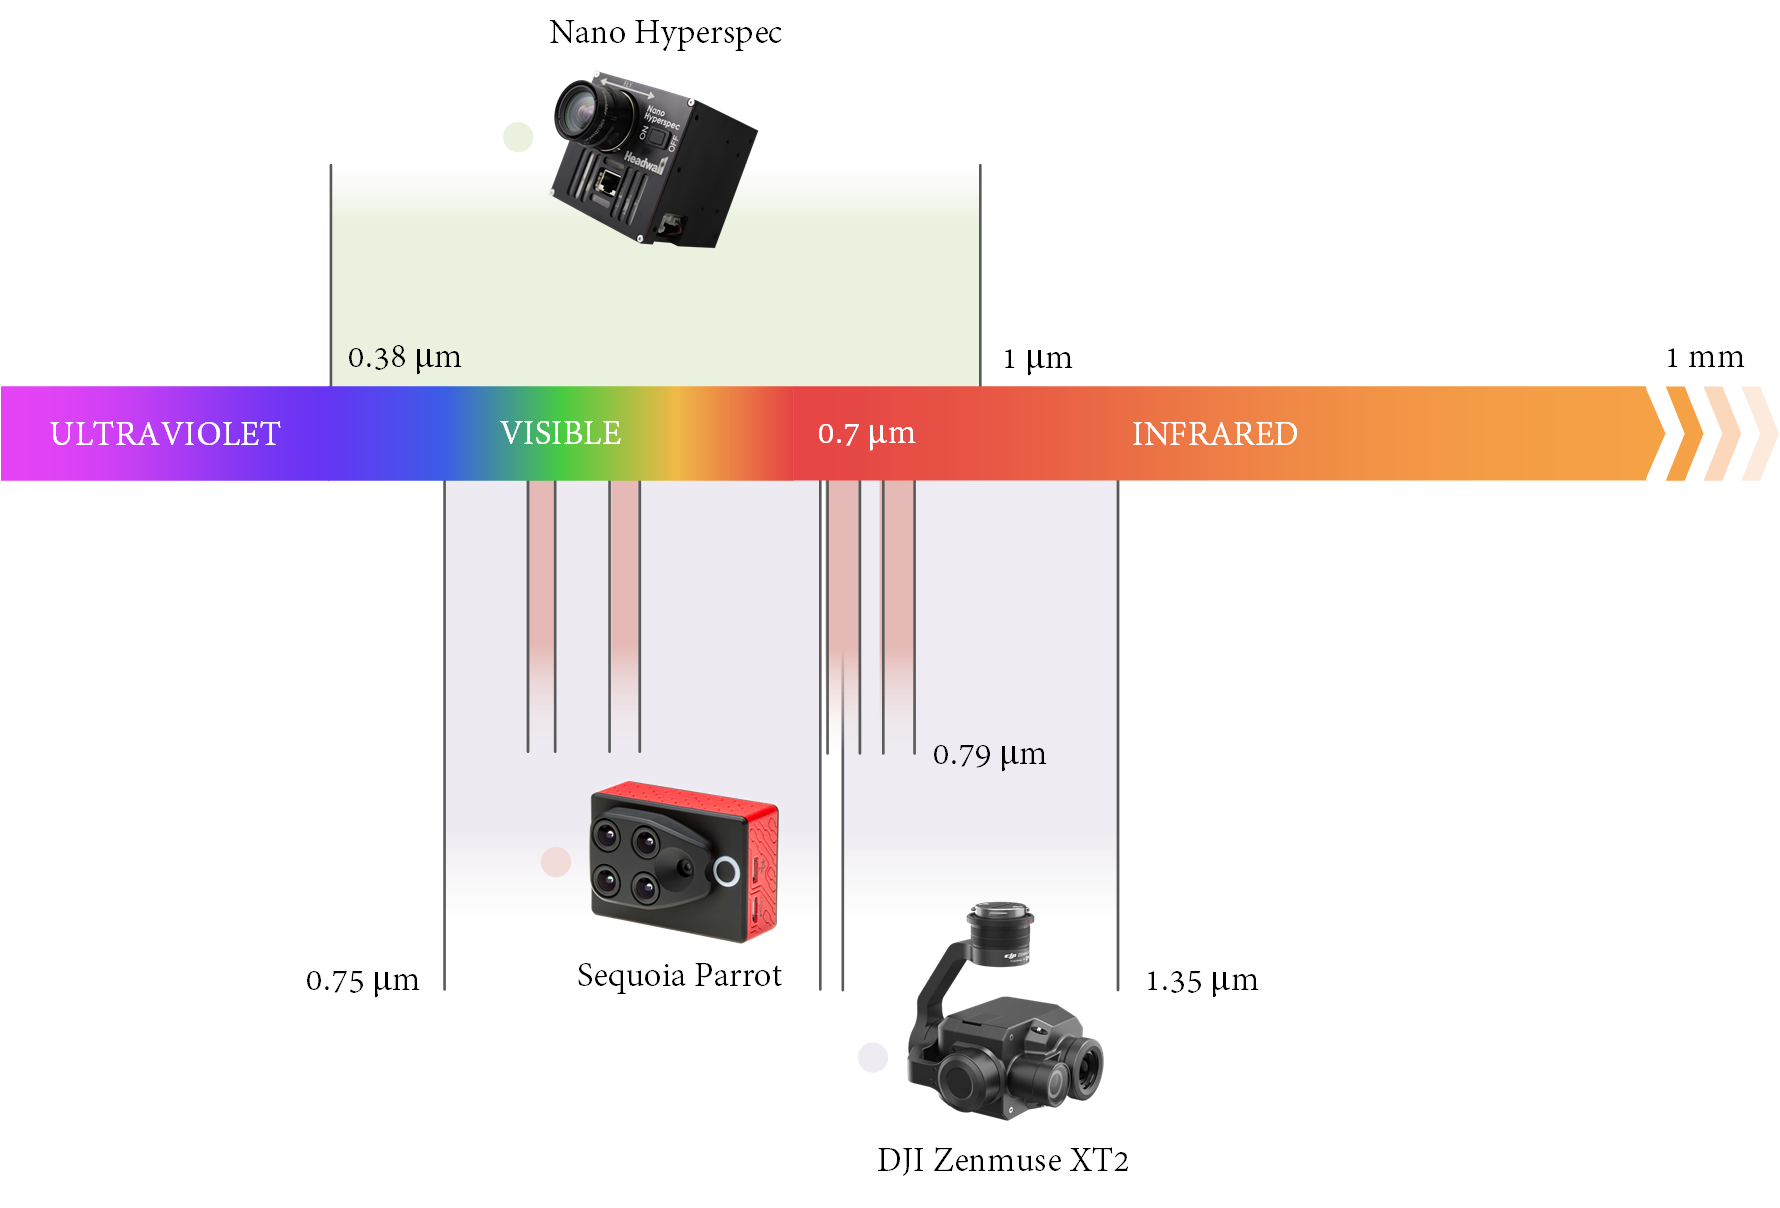
\includegraphics[width=.9\linewidth]{figs/context/spectra_devices.png}
	\caption{Available spectra from three different devices utilized for collecting \acrshort{uas}-based imagery. }
    \label{fig:available_spectra}
\end{figure}

This section is structured as follows. First, the fusion of images and point clouds is explored to match pairs of images, point clouds or images and point clouds. Rather than fusing visible imagery, which is the foundational core of photogrammetry, the focus here is on the fusion of visible imagery and other data sources. Then, the augmentation of remotely collected datasets is explored to generate point clouds from metropolitan and rural environments. Finally, the previously fused and generated data is applied to several case studies: the planning of scans in indoor scenarios, the phenotyping of grapevines and the inspection of archaeological sites in seek of buried remains.

\section{Fusion of information}

\subsection{Motivation}

The content of this section is principally obtained from the manuscript \textbf{"Remote sensing image fusion on 3D scenarios: A review of applications for agriculture and forestry"}. Although the aim of this publication was to revise work on the fusion of data for agriculture and forestry, only a few works related to this topic achieved 3D reconstruction with their own pipeline. Instead, most studies coped with 2D and 3D reconstruction using third-party software. Therefore, the domain of application was enlarged and a discussion was established for every revised methodology about the degree of applicability to agriculture and forestry areas.

The volume of remote sensing data is rapidly increasing and many real-world scenarios are currently being replicated by the generation of virtual models in 3D. The multi-source data integration and the 3D representation of surveyed areas is a hot research topic in the field of geoscience and remote sensing and has attracted the attention of both industry and academia. Focusing on natural and environmental areas, it has many prospective applications in smart agriculture \cite{jurado_multispectral_2020, padua_vineyard_2019, poblete_discriminating_2021}, forestry and nature preservation \cite{almeida_monitoring_2021, guimaraes_forestry_2020, heckel_predicting_2020, schiefer_mapping_2020} and monitoring \cite{maimaitijiang_crop_2020}. Initially, the acquisition of remote sensing data required costly sensors mounted on complex platforms. Likewise, the surveying procedure and data processing were labour-intensive and time-consuming. Observed scenarios were mainly represented in 2D maps and orthophotos, after applying manual processes to correct the image distortion \cite{vong_how_2021}. In this field, significant advances have been achieved by the development of efficient methodologies for data acquisition and processing, as well as the production of new sensor capabilities and aerial platforms. Accordingly, extensive research is currently being carried out focusing on multi-source data fusion and image mapping on 3D models.

In this context, the proliferation of \acrshort{uas} as versatile and cost-efficient platforms to acquire multi-source data has enabled the detailed characterization of large scenarios, even with difficult accessibility. Undoubtedly, \acrshort{uas} technology plays an important role in multidisciplinary research benefitting from unprecedented temporal, spatial and spectral resolution, acquired from multiple perspectives in a non-intrusive way.

Although data fusion can be performed over pairs of images, most applications use this as a first step towards approaching 3D reconstructions. From here, primitives from 3D representations, obtained with a single data source, are easily back-projected to another data source. Thus, stack-based representations from image matching also lead to point clouds with multiple layers. Besides the benefits of 3D models in visual inspections, these are significantly more valuable when combined with \acrshort{rgb}, multispectral, hyperspectral and thermal data. The fusion of these data and 3D geometry depicting natural and artificial surfaces brings a deep knowledge of our environment. Figure \ref{fig:scopus_point_clouds} offers a vision of how 3D modelling has been gaining interest in data sources beyond the visible spectral range. The Scopus searches were the following: $(p_1 \lor p_2 ... \lor p_n) \land ((\textit{point} \hspace{1mm} \land \hspace{1mm} \textit{cloud}) \lor (\textit{3D} \hspace{1mm} \land \hspace{1mm} \textit{modelling}))$, with $p_i$ being different names that identify a data source (e.g., visible and \acrshort{rgb}).

\begin{figure}[ht]
    \centering
    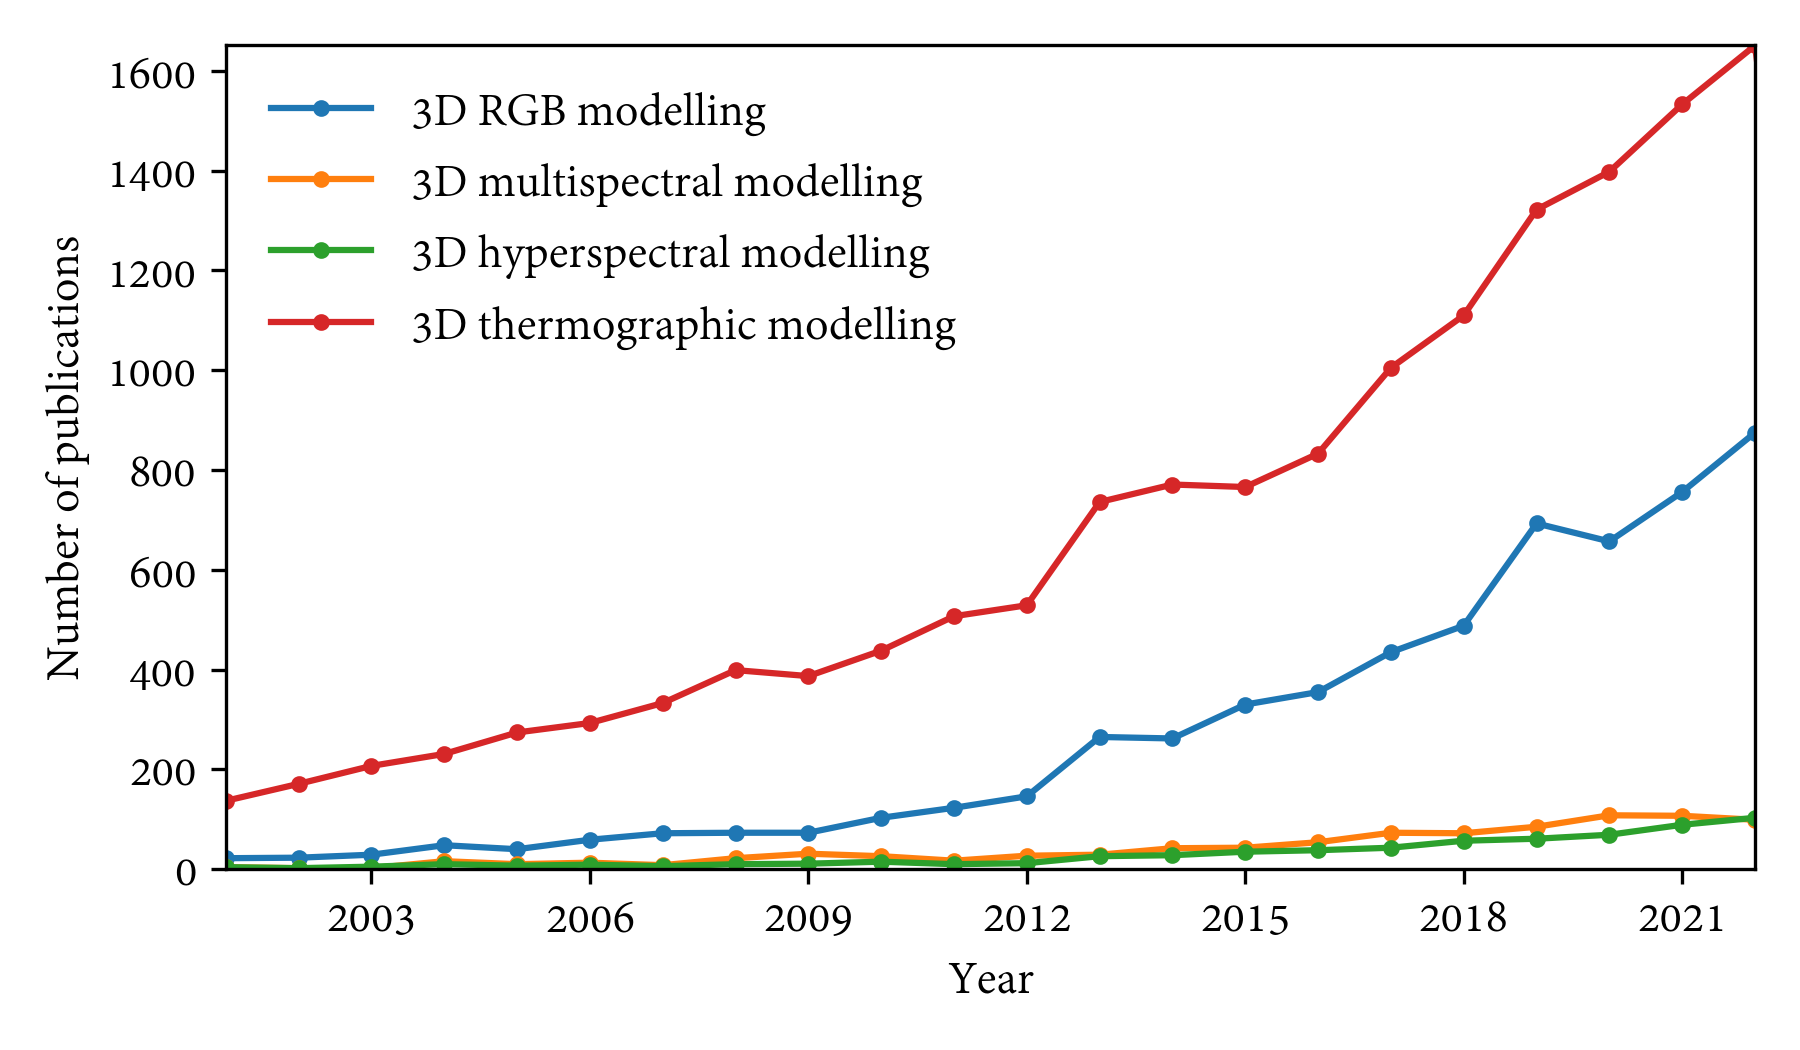
\includegraphics[width=\linewidth]{figs/context/3d_modelling.png}
	\caption{Number of publications related to visible, multispectral, hyperspectral and thermographic 3D modelling, from 2000 to the current year. }
	\label{fig:scopus_point_clouds}
\end{figure}

The integration of multiple data sources, in combination with 3D reconstructions, is still challenging since each dataset is obtained with a different mechanism (global or rolling shutter, push broom sensors, etc.), intrinsic and extrinsic parameters, distortion and resolution. Therefore, fusing multiple datasets is not trivial and demands high computational efforts that can be alleviated with \acrshort{gpgpu}. In the following subsections, the main contributions to the fusion of visible, thermographic, multispectral and hyperspectral data are summarized. First, the fusion of 2D data is reviewed and then, the combination of imagery and point clouds is revised. Both sections are split into works related to thermal, multispectral and hyperspectral data. 

\subsection{Image matching}

\subsubsection{Thermal infrared imaging}

Consumer-grade \acrshort{ir} cameras are not prohibitive, at the expense of having lower resolution and a higher number of defects. Sledz et al. \cite{sledz_thermal_2018} reported several sources of noise causing \acrshort{ir} images to have a blurred and smoothed-out appearance. Among these, environmental conditions and non-uniformity of focal plane arrays (\acrshort{fpa}) were highlighted \cite{javadnejad_photogrammetric_2020}. Furthermore, the radiation of a surface is captured by several detector elements, as energy spreads to the surroundings \cite{vollmer_infrared_2017}. \acrshort{uas} platforms are less affected by the attenuation from energy dispersion and atmospheric absorption, though this is a well-known problem in thermography \cite{gonzalez_thermal_2019, vollmer_infrared_2017, quattrochi_thermal_1999}.

Amongst works addressing matching visible and thermal imagery, only a few consider that both data sources are perfectly overlapped as collected \cite{hou_fusing_2021, stojcsics_high_2018}. However, this scenario is not frequent; instead, visible and thermal imagery record slightly different areas of interest, even for images co-acquired by dual devices. This is caused by minor differences in triggering timestamps, the platform's movement and the device calibration, which may degrade over time. 

The most frequent approaches for \acrshort{ir} image registration are depicted in Figure \ref{fig:fusion_data_03}. One of the main concerns is the selection of the most appropriate feature descriptor. The reviewed literature shows a higher preference for edge detection algorithms, such as Canny and Sobel operators \cite{hoegner_3d_2016, hoegner_evaluation_2016}, over conventional feature descriptors, including the Scale-invariant feature transform (\acrshort{sift}), Speeded-Up Robust Features (\acrshort{surf}) and Oriented FAST and rotated BRIEF (\acrshort{orb}) (Figure \ref{fig:feature_descriptors}). In this regard, Hoegner et al. \cite{hoegner_evaluation_2016} enhanced the edge detection by solely conserving prominent edges with the Hough transform \cite{hoegner_evaluation_2016}. However, edge detection algorithms are not as appropriate for forestry and rural scenarios, as depicted in Figure \ref{fig:feature_detection}. Previous work has also coped with image matching on the frequency domain, with the aim of handling nonlinear colourimetric differences between visible and \acrshort{ir} imagery. Lin et al. \cite{lin_fusion_2019} implemented the Radiance Invariant Feature Transform (\acrshort{rift}) \cite{lin_fusion_2019}, followed by a suppression of mismatches with Random Sample Consensus (\acrshort{ransac}).

From here, projecting \acrshort{ir} imagery in 3D reconstructions is trivial; 3D points are efficiently projected into \acrshort{rgb} images, which have already been matched with thermography. Figure \ref{fig:fusion_data_03} illustrates the image-matching algorithms and how these help in the later 3D reconstructions. 

\begin{figure*}[ht]
	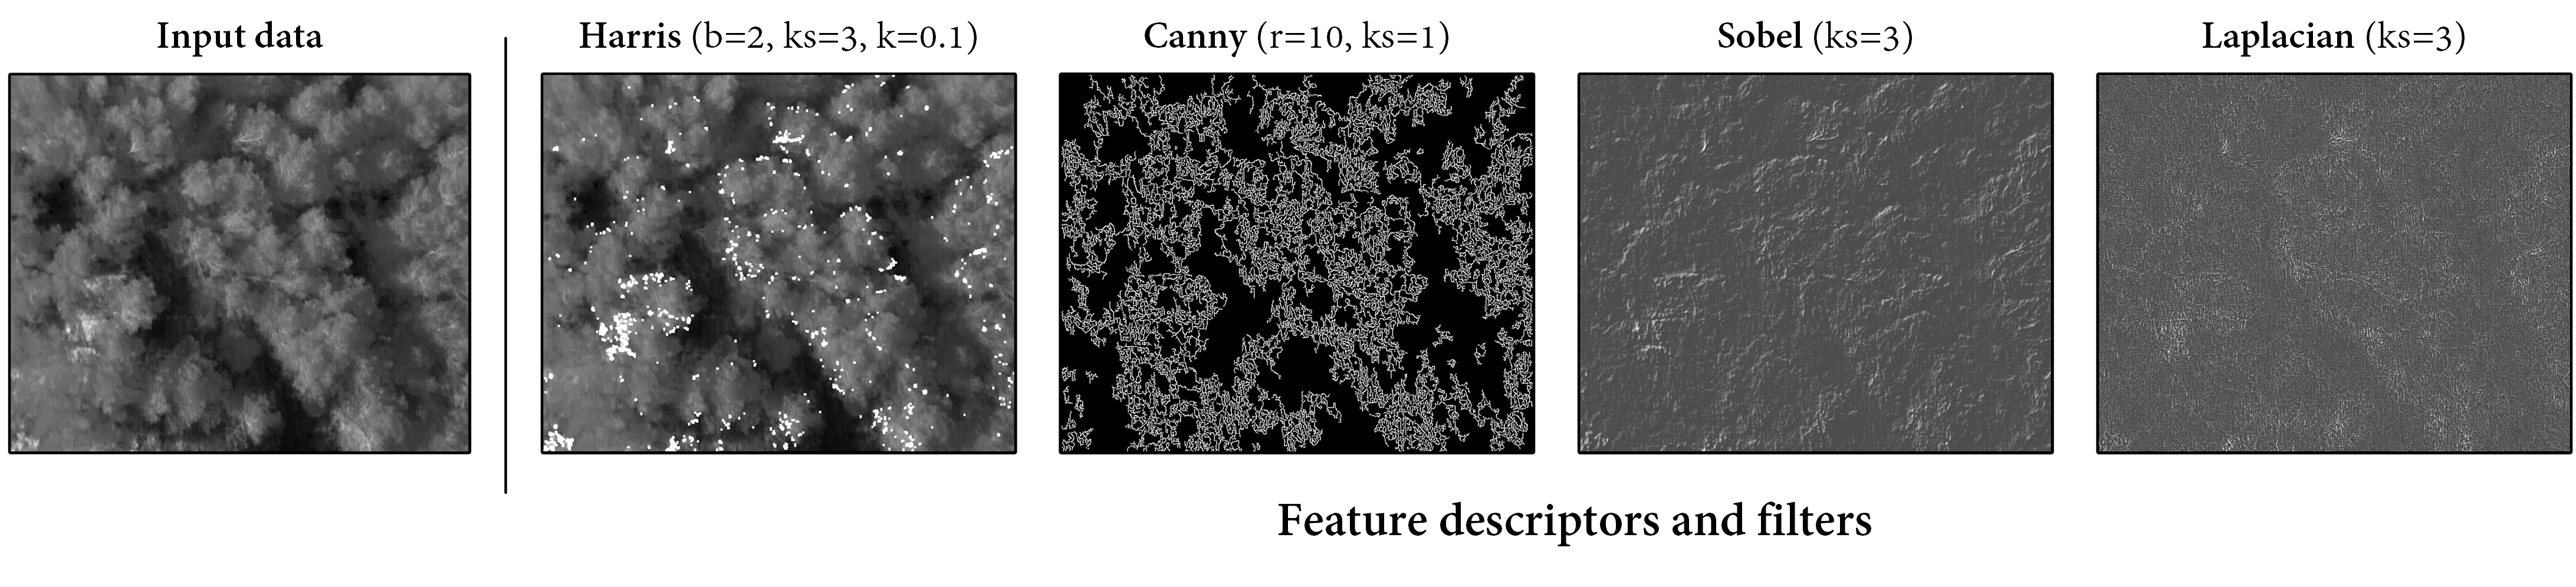
\includegraphics[width=\linewidth]{figs/context/feature_detection.png}
	\caption{Comparison of edge-based feature descriptors frequently used in image registration algorithms. These are less likely to work for vegetation as no relevant features are found. $\textit{ks}$ refers to kernel size, the ratio is presented as $\textit{r}$, and $\textit{k}$ is a free parameter on the Harris detector. The brightness of the two first images is increased to improve the visualization.}
    \label{fig:feature_detection}
\end{figure*}

Instead of using colourimetric data, other studies have proposed a calibrated system with multiple devices. Thermographic imagers are frequently combined with \acrshort{rgb} cameras \cite{javadnejad_photogrammetric_2020, landmann_multimodal_2019, adan_fusion_2017} and \acrshort{lidar} \cite{adan_fusion_2017, hoegner_fusion_2018}. The calibration of dual-sensor systems is performed by estimating the translation (lever-arm) and rotation (boresight) matrices that represent how these sensors correlate (see Figure \ref{fig:fusion_data_04}). Calibration is frequently performed by identifying features visible in several images, either following a supervised or semi-supervised approach. However, the calibration of systems with multiple sensors was proven to perform worse in inexpensive, consumer-grade thermal cameras \cite{javadnejad_photogrammetric_2020}. Constructing a checkerboard calibration panel and marking features on it is particularly tough using \acrshort{ir} data \cite{javadnejad_photogrammetric_2020} since it lacks sharp edges. However, these systems with multiple devices have the advantage of rapidly fusing 2D and 3D data simultaneously once calibrated.

\begin{figure*}[ht]
	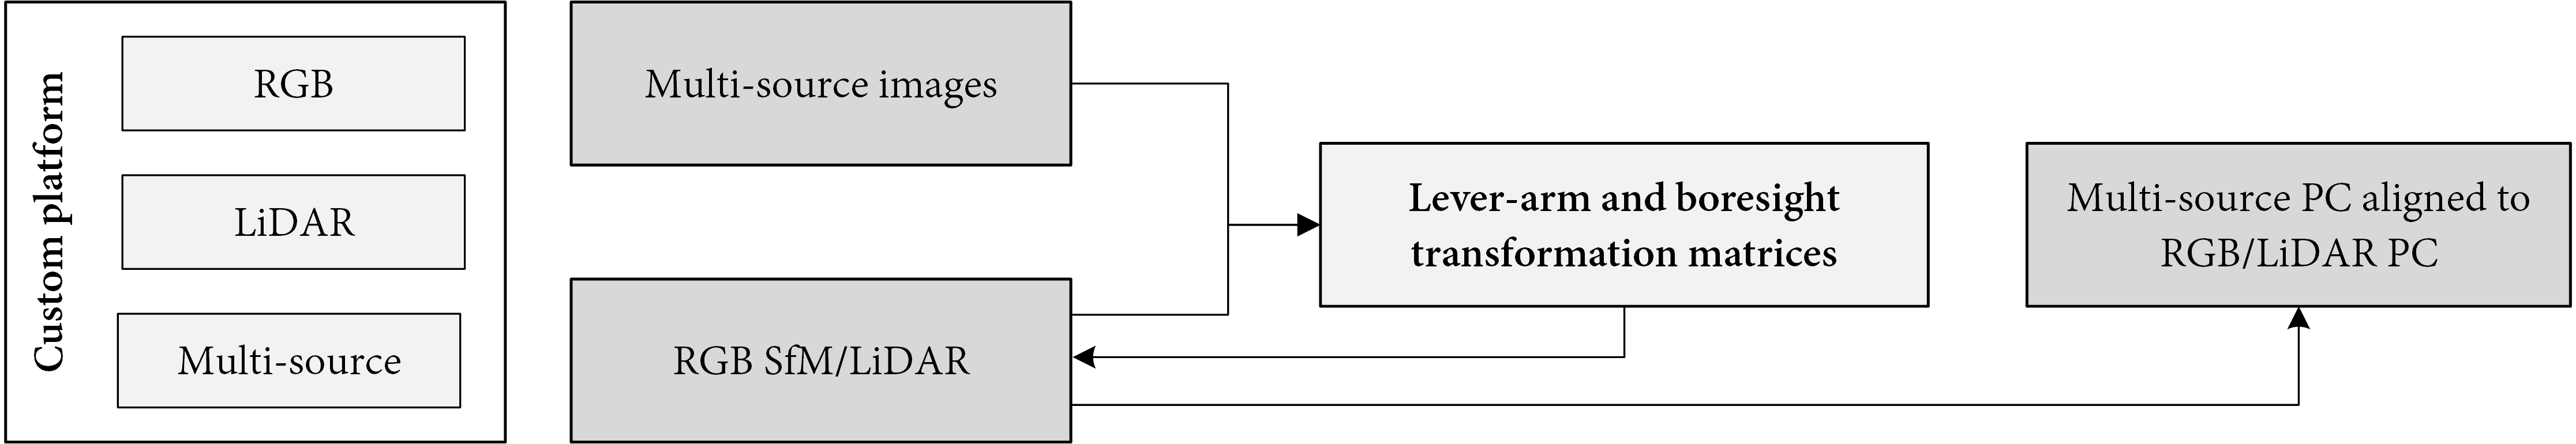
\includegraphics[width=\linewidth]{figs/context/fusion_04.png}
	\caption{Systems with multiple sensors are calibrated with the aim of projecting multiple data sources into a single coordinate system.}
    \label{fig:fusion_data_04}
\end{figure*}

\subsubsection{Multispectral imaging}

Unlike \acrshort{ir}, multispectral datasets are composed of several bands in the visible and infrared wavelengths. These bands are more likely to not record the exact same area of interest, influenced by different positioning of lenses, the platform's movement and the calibration of each individual imager, which deteriorates over time. Shen et al. \cite{shen_multi-modal_2014} introduced an image-matching solution based on a descriptor measuring the degree of matching for every pixel. Other works used the orientation embedded in the image metadata to correct the misalignment \cite{jhan_band--band_2016}, and the error of these parameters was reduced with \acrshort{ransac} \cite{jhan_investigation_2017}. Similarly to \acrshort{ir} image-matching, the \acrshort{surf} \cite{sedaghat_high-resolution_2019} and \acrshort{sift} \cite{saleem_robust_2014} feature descriptors have also been applied to multispectral datasets. According to Tsai and Lin \cite{tsai_accelerated_2017}, the \acrshort{sift} method outperformed other algorithms in terms of quality of results and efficiency.

\begin{figure}[ht]
	\includegraphics[width=\linewidth]{figs/context/feature_extraction.png}
	\caption{Comparison of two traditional feature descriptors and matching algorithms: \acrshort{sift} and  \acrshort{orb}. In this example, both are used to match multi-view sequences of the same scene.}
    \label{fig:feature_descriptors}
\end{figure}

\subsubsection{Hyperspectral imaging}

Hyperspectral sensors collect the light intensity in a large number of contiguous spectral bands, typically ranging from a few tens to several hundred. Every pixel stores the spectral response of one or multiple materials, thus helping to understand images and monitor scenarios. \acrshort{hsi} comprises several scan geometries, already explained in Section \ref{sec:fundamentals_optical_imaging_geometry}, although the vast majority of works are based on the push broom technology (see Figure \ref{fig:hyper_scan_geometry}). Push broom sensors include a set of 2D detectors that simultaneously sample all the points along a line. The area of interest is surveyed by translating the platform in the direction orthogonal to such a line. This scanning technology enables the simultaneous acquisition of every wavelength in a pixel, thus facilitating and reducing the post-processing of hypercubes. It is also worth noting that the type of sensor greatly affects field operations, processing performance and the quality of the final product \cite{adao_hyperspectral_2017}. 

With this in mind, the main objective of fusing hyperspectral data with other data sources is to correct the geometric distortions, and therefore, the other data source is the reference without geometric errors. In this regard, Jurado et al. \cite{jurado_efficient_2021} proposed a method for matching hyperspectral and high-resolution \acrshort{rgb} imagery. Hyperspectral swaths were split into smaller fragments, and the \acrshort{orb} feature descriptor was used to find common features. From here, it was estimated whether the resulting transformation matrix was feasible or not by measuring the distance of control points in hyperspectral (after projection) and \acrshort{rgb} imagery. Otherwise, a smaller partition of the swath was used until a stable alignment was achieved or the current fragment could be further split. Previously, Angel et al. \cite{angel_automated_2020} aligned hyperspectral and \acrshort{rgb} images by applying \acrshort{surf} and discarding mismatches with a variant of \acrshort{ransac}, Maximum Likelihood Sample Consensus (\acrshort{mlsac}). Also recently, Akhoundi Khezrabad et al. \cite{akhoundi_khezrabad_new_2022} avoided the use of \acrshort{gcp}s by simultaneously recording a video together with hyperspectral data. \acrshort{sift}, \acrshort{ransac} and Spectral Angle Mapper (\acrshort{sam}) were applied to the geometric correlation. Note that \acrshort{sam} helps to discard mismatches since it measures how similar are two spectral signatures regardless of their scale.

\subsection{3D reconstructions}

\subsubsection{Thermographic imaging}

The majority of outdoor \acrshort{ir} datasets come from \acrshort{uas} platforms, despite terrestrial and indoor collections also being frequent. Lin et al. \cite{lin_fusion_2019} and Stojcsics et al. \cite{stojcsics_high_2018} collected \acrshort{ir} data from a hand-held camera, whereas Zhu et al. \cite{zhu_fusion_2021} recorded both \acrshort{ir} and \acrshort{lidar} from a vehicle coupled with multiple sensors. Adán et al. \cite{adan_towards_2020} used a robotic platform to autonomously navigate and scan indoor environments. Previous work also exploited the use of custom systems that are geometrically calibrated by describing the lever-arm between multiple sensors \cite{javadnejad_photogrammetric_2020, hoegner_fusion_2018}. This calibration is achieved by collecting multiple images depicting a known pattern, typically a checkerboard \cite{javadnejad_photogrammetric_2020} or landmarks with peculiar reflectivity \cite{adan_fusion_2017}. 

\begin{figure*}[ht]
	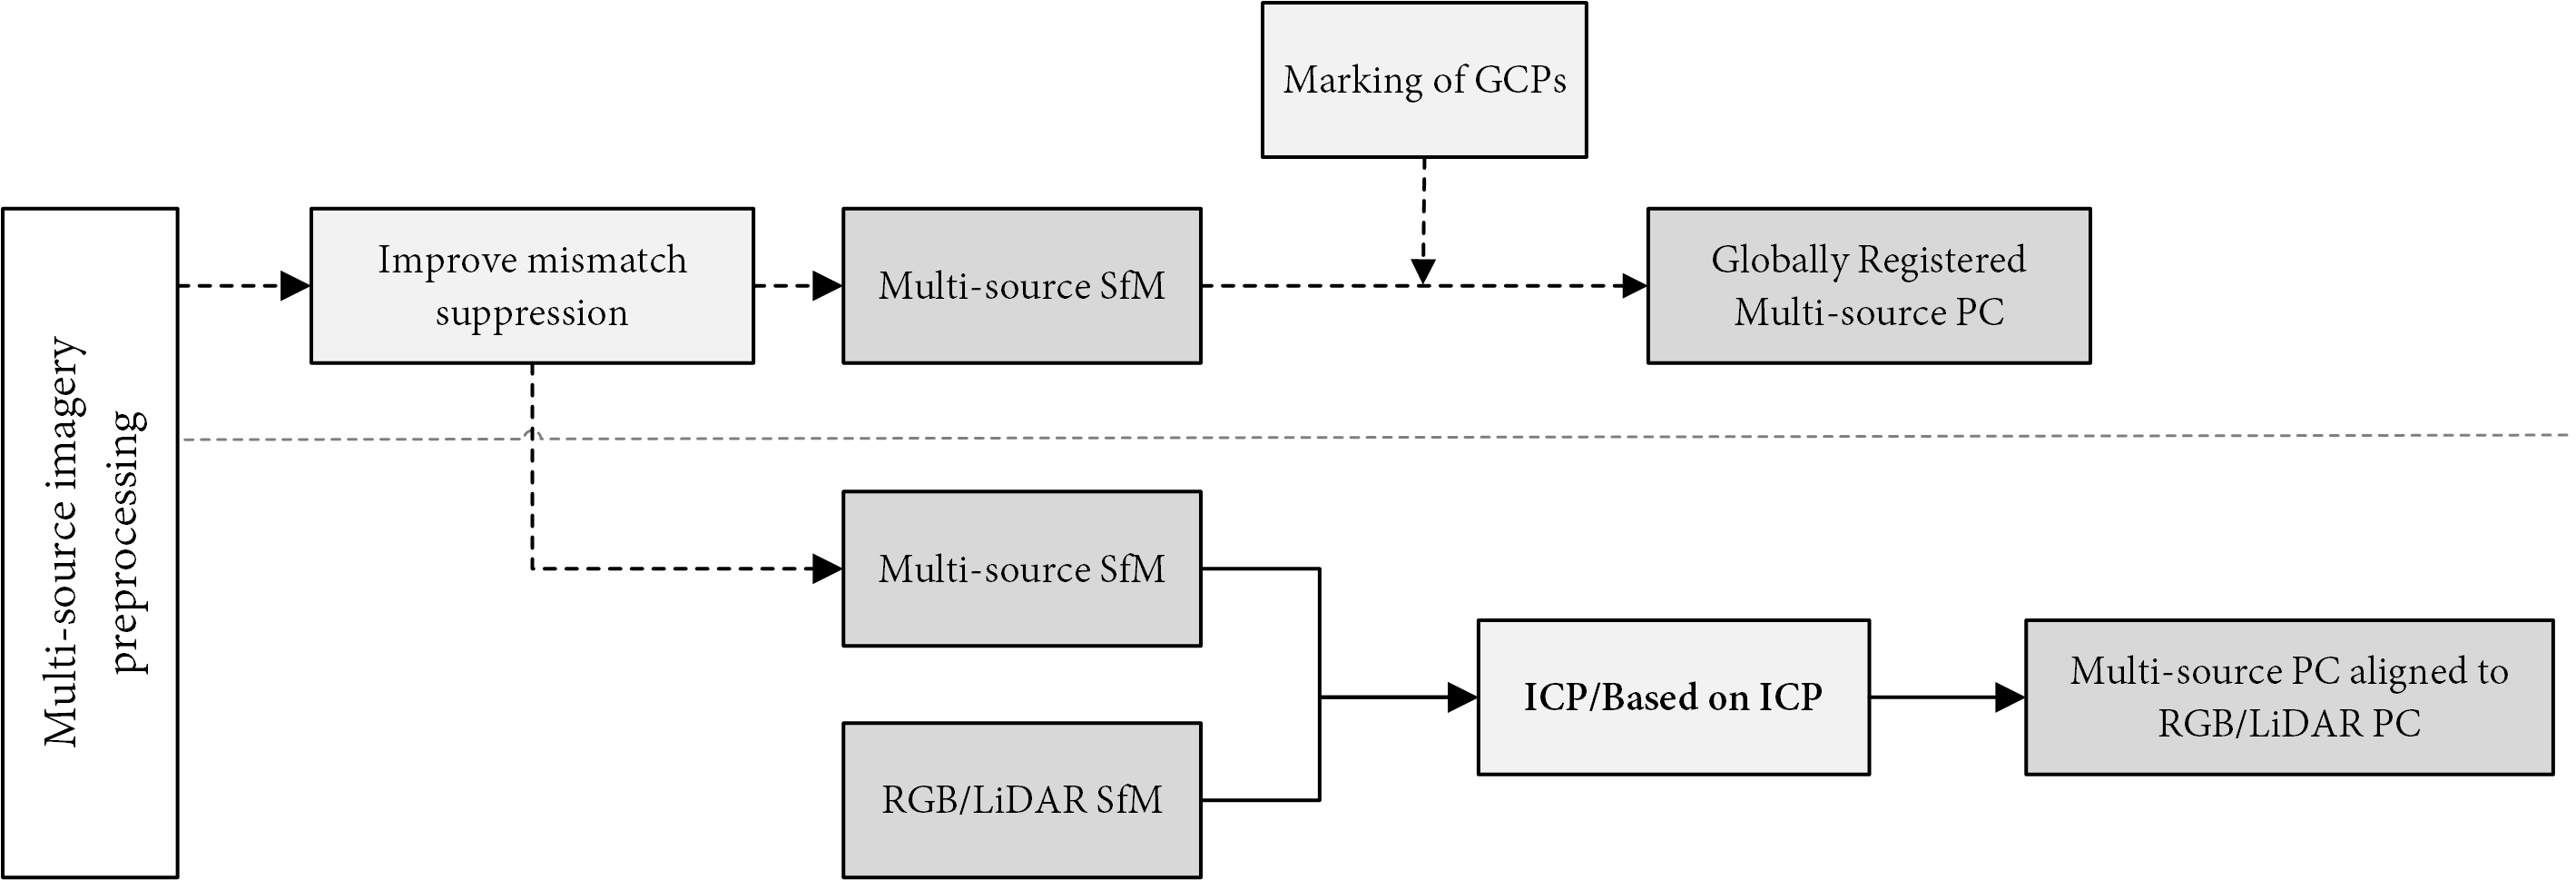
\includegraphics[width=\linewidth]{figs/context/fusion_01.png}
	\caption{Two different approaches for reconstructing 3D \acrshort{ir} models. First, \acrshort{sfm} is used over visible and \acrshort{ir} datasets, whereas the second procedure estimates the rigid transformation that aligns two point clouds. }
    \label{fig:fusion_data_01}
\end{figure*}

In spite of the low resolution of \acrshort{ir} imagery, previous work has extensively applied photogrammetry to reconstruct \acrshort{ir} point clouds \cite{dahaghin_precise_2021, dahaghin_3d_2019, gonzalez_thermal_2019, grechi_3d_2021, webster_three-dimensional_2018, sledz_thermal_2018, kniaz_thermal_2018, hoegner_mobile_2018, zheng_thermal_2020, guilbert_fusion_2020}. This paradigm is illustrated in Figure \ref{fig:fusion_data_01}. Among other factors, this approach is very frequent since \acrshort{sfm} is part of notable commercial and open-source software and thus is particularly easy to apply. Some of these third-party solutions are Pix4Dmapper \cite{zheng_thermal_2020}, Agisoft Metashape \cite{grechi_3d_2021, guilbert_fusion_2020, lin_fusion_2019, macher_combination_2019}, Autodesk Recap 360 \cite{lafi_3d_2017} and Zephyr \cite{maset_photogrammetric_2017, clarkson_thermal_2017}. Although photogrammetry is trivial to apply from third-party software, \acrshort{ir} imagery has defects and limitations that harden this process, for instance, on the retrieval of tie points during feature detection \cite{lin_fusion_2019}. Consequently, resulting point clouds are more likely to be scarce, less precise and more geometrically inaccurate due to noise, gaps and incorrectly estimated elevation \cite{kong_3-d_2018}. Photogrammetry is similarly problematic for environments showing repetitive patterns and uniform textures, e.g., buildings and vegetation \cite{lin_fusion_2019, jarzabek-rychard_supervised_2020}, even for other data sources. On the other hand, geometrical inaccuracies can be mitigated using \acrshort{gcp}s. However, the marking of \acrshort{gcp}s is more challenging in thermography due to the low resolution and colour contrast \cite{sledz_thermal_2018}. Still, previous work has explored the placement of \acrshort{gcp}s without further considerations to reconstruct \acrshort{ir} point clouds \cite{dahaghin_precise_2021, gonzalez_thermal_2019, zheng_thermal_2020, sledz_thermal_2018}. Boesch et al. \cite{boesch_thermal_2017} and Nishar et al. \cite{nishar_thermal_2016} overcome the limited visibility of \acrshort{gcp}s by using metal-coated materials with low emissivity, in contrast with the surrounding vegetation. In this regard, Figure \ref{fig:gcps_thermography} shows the poor visibility of non-metal-coated \acrshort{gcp}s when they are surrounded by vegetation (with similar radiation) instead of bare soil. 

\begin{figure*}[ht]
	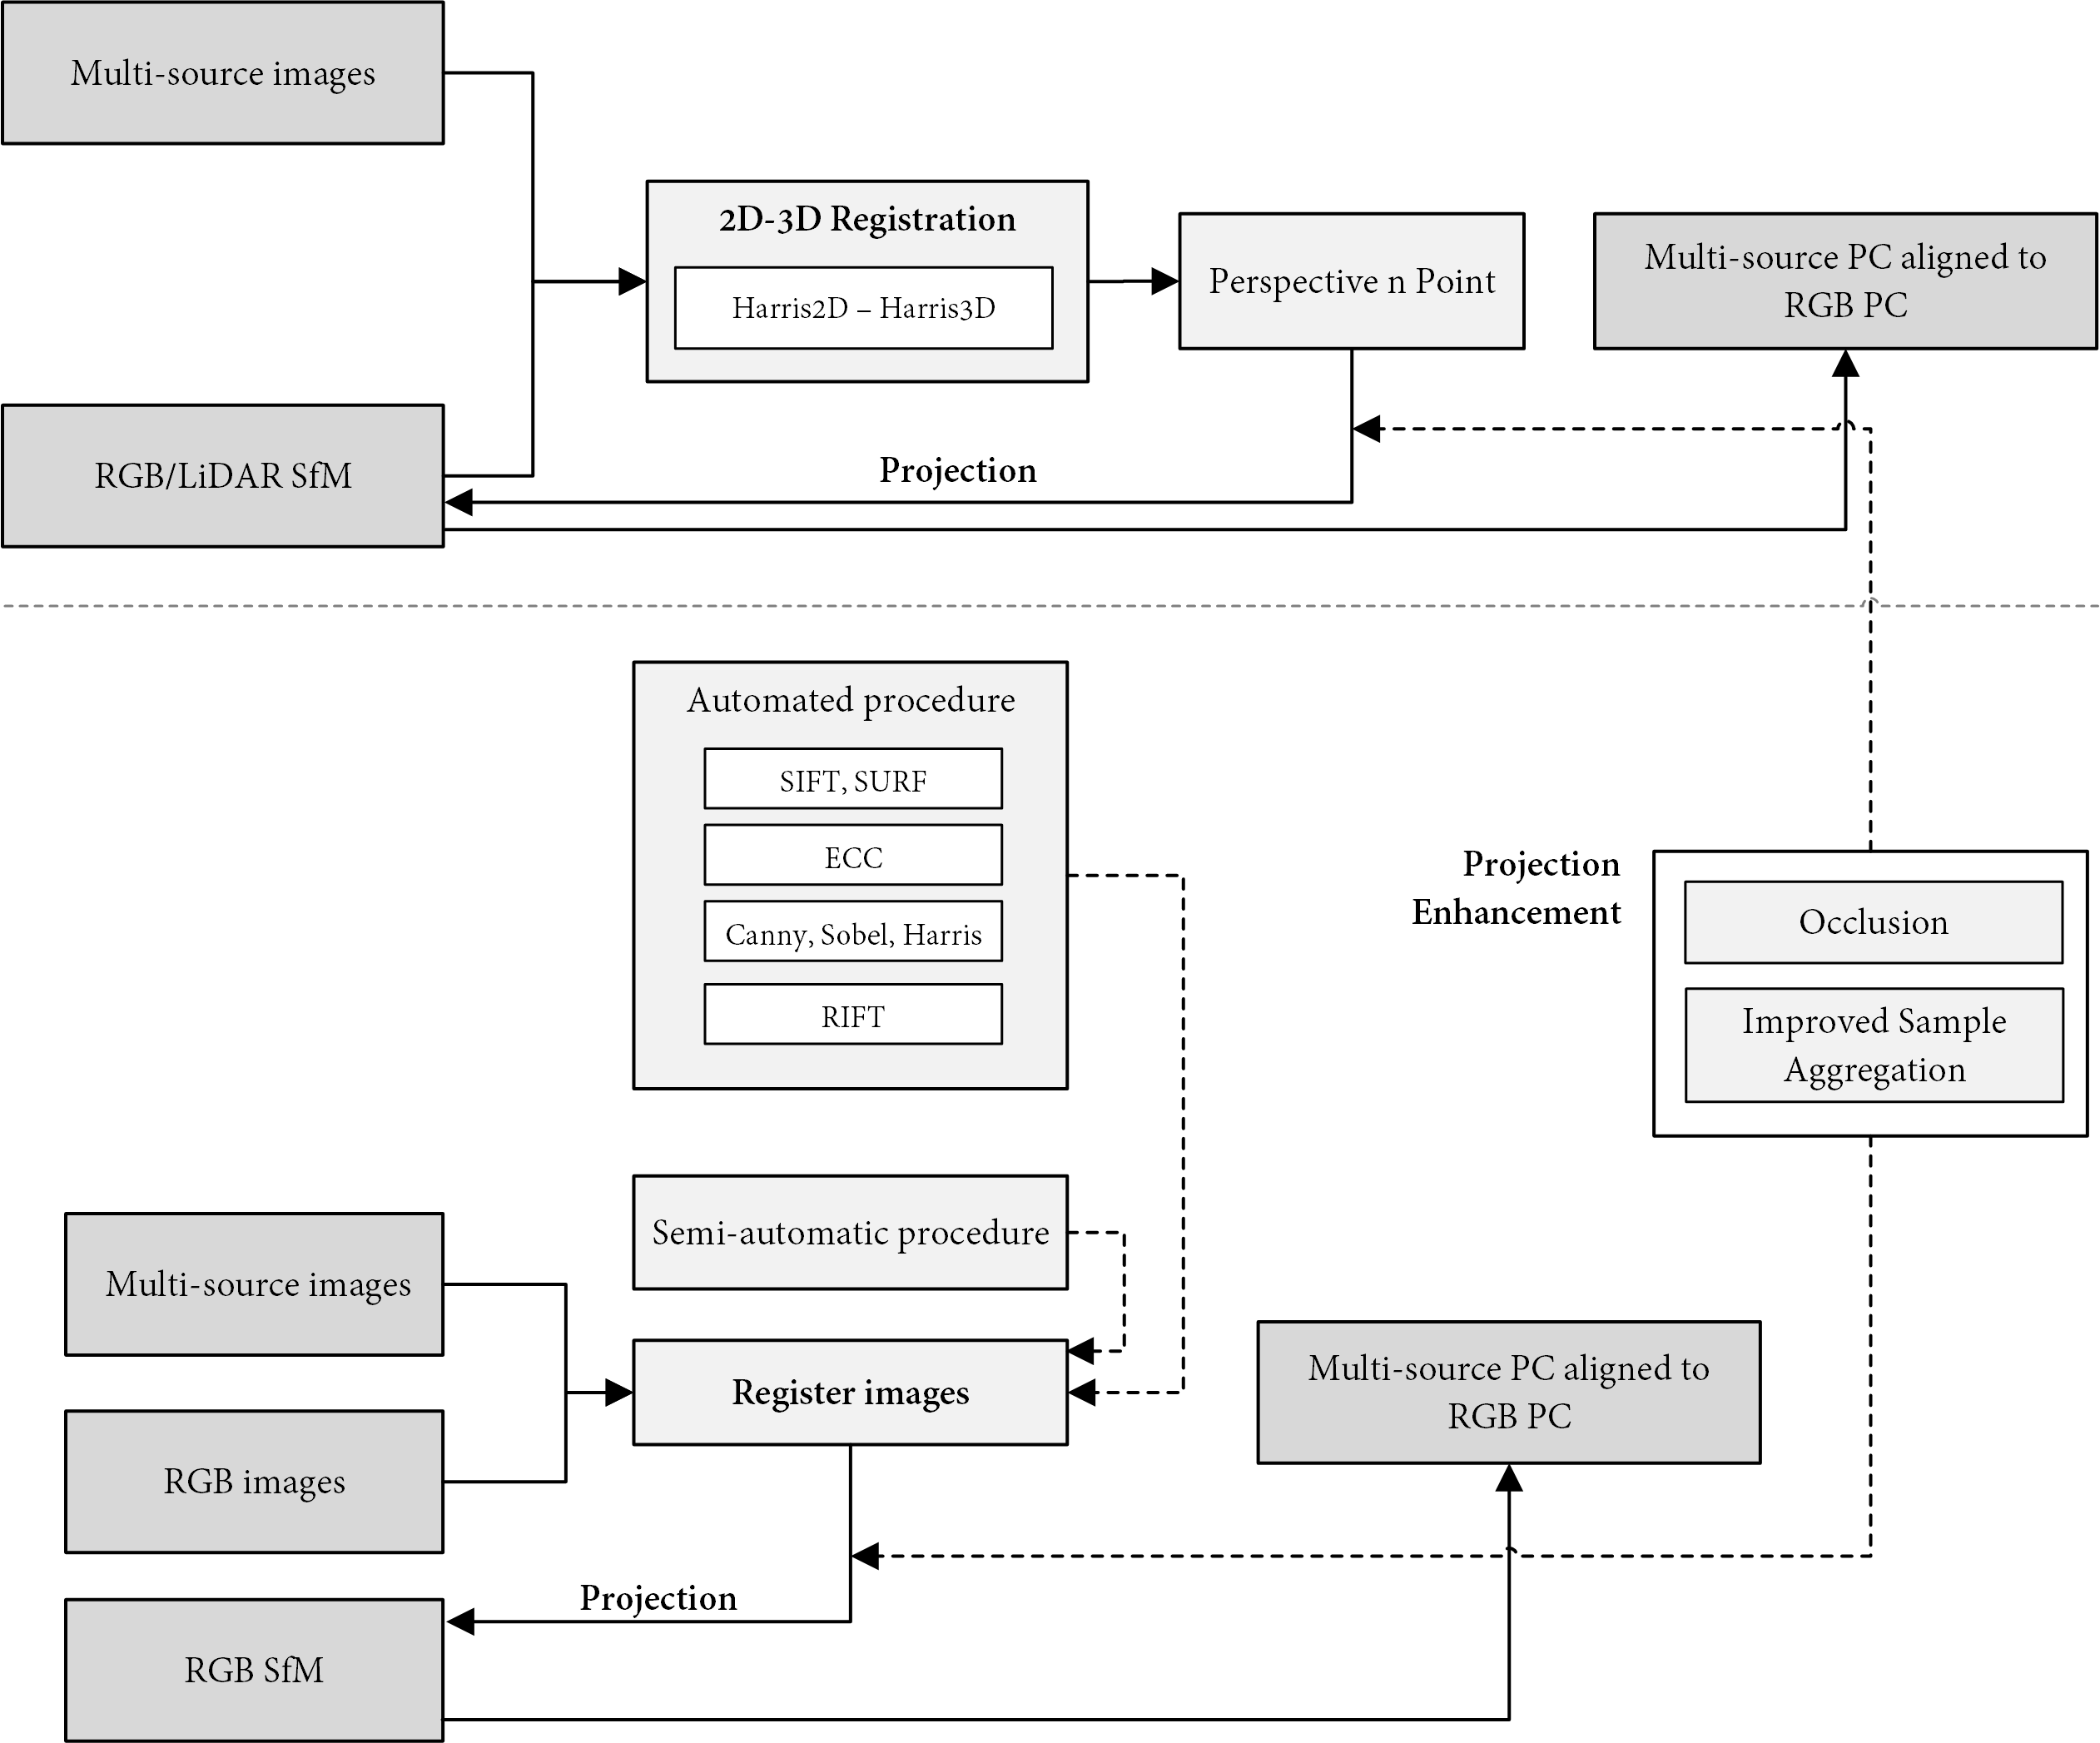
\includegraphics[width=\linewidth]{figs/context/fusion_03.png}
	\caption{Two different methods for reconstructing 3D point clouds. First, images are mapped into a baseline point cloud once 2D and 3D features are correlated and used to estimate pose parameters. In the second approach, features are only sought in 2D to compute the transformation matrix between \acrshort{rgb} imagery and other data source. }
    \label{fig:fusion_data_03}
\end{figure*}

\begin{figure}[ht]
	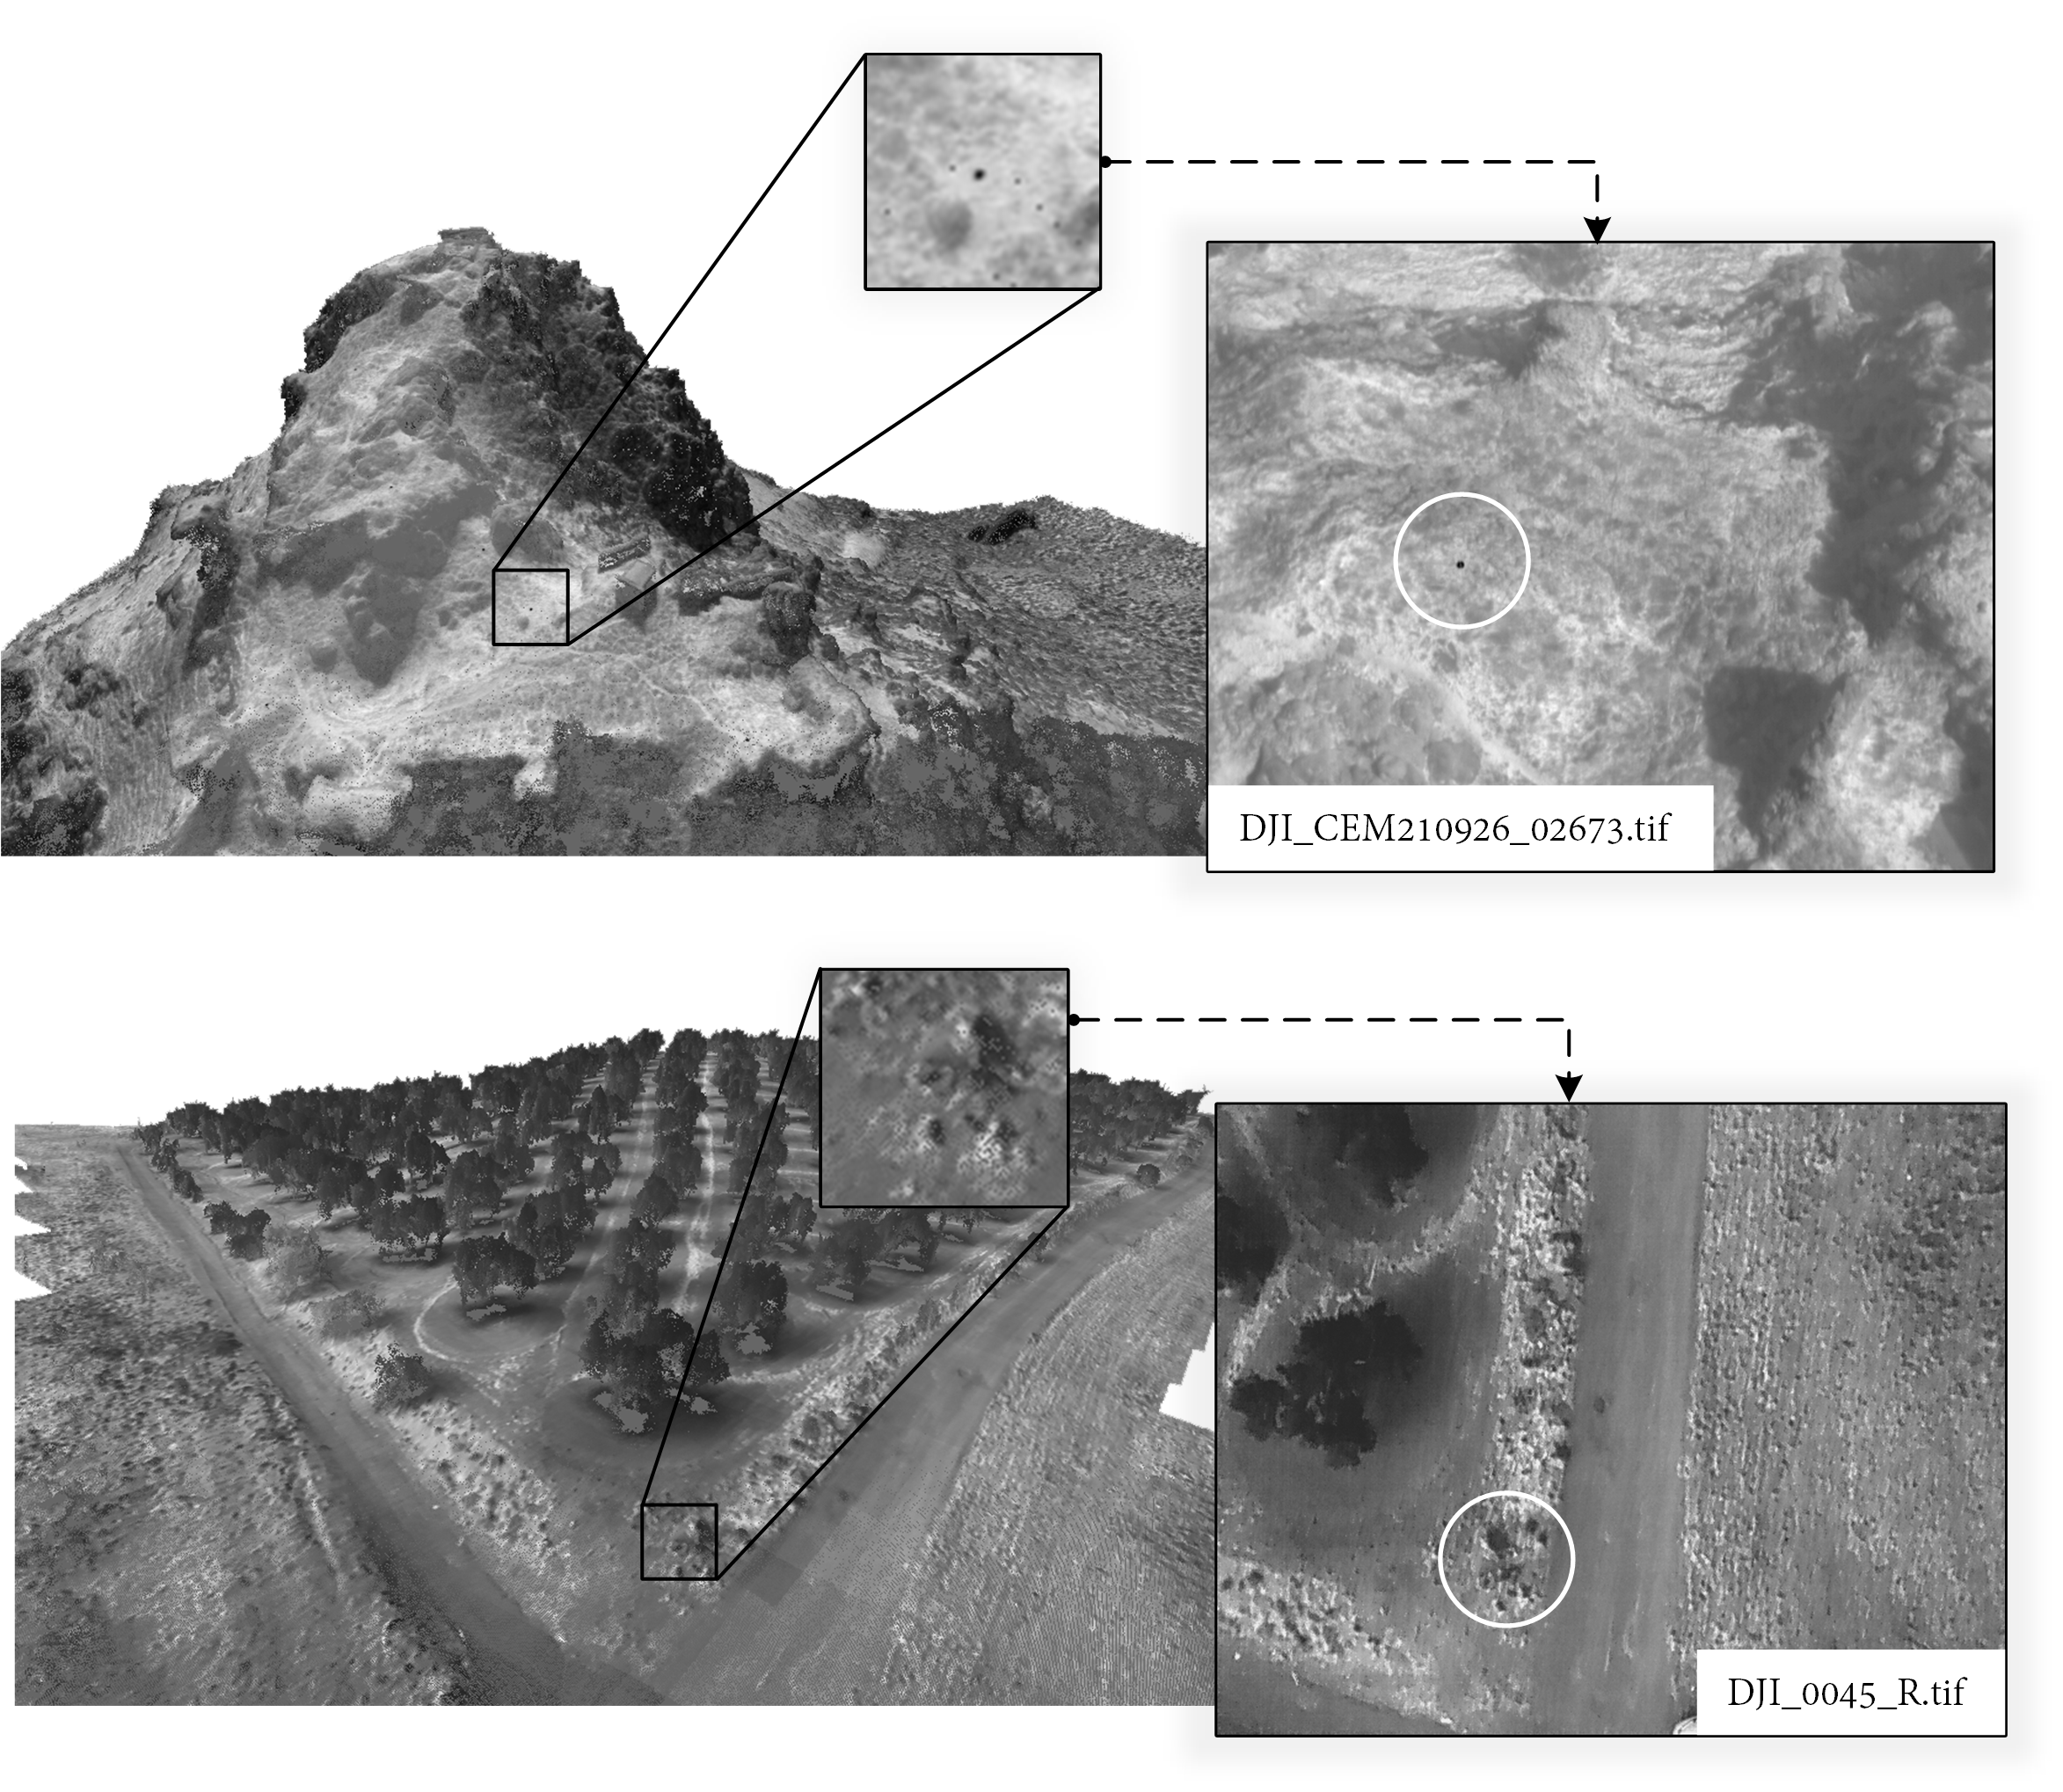
\includegraphics[width=\textwidth]{figs/context/gcps.png}
	\caption{Non-metal-coated \acrshort{gcp}s made of plastic under two different scenarios. \acrshort{gcp}s are barely noticeable in the second scenario since the surroundings have a similar temperature. In the first scenario, they are significantly more visible to the naked human eye since the surroundings are bare soil. }
    \label{fig:gcps_thermography}
\end{figure}

Another revised approach is to improve some of the stages of \acrshort{sfm} with the help of other data sources. For instance, the External Orientation Parameters (\acrshort{eop}) could be estimated from visible datasets that have larger dimensionality and higher accuracy \cite{jo_dense_2021}. Maes et al. \cite{maes_optimizing_2017} estimated the \acrshort{ir} camera parameters using the Brown-Conrady distortion model. The temperature was corrected by decoupling the influence of air temperature in multiple flights. Also, the image geopositioning was improved with the onboard \acrshort{gps} and Global Navigation Satellite System (\acrshort{gnss}). To overcome the limitations imposed by the \acrshort{sfm}'s keypoint detection, previous work has explored other algorithms aimed at extracting features and suppressing mismatches. In this regard, Kong et al. \cite{kong_3-d_2018} applied \acrshort{knn} to remove evident mismatches, followed by a modification of \acrshort{ransac} where the temperature was used to tell mismatches apart. 

Instead of only using \acrshort{ir} data, the fusion of several data sources, with one of them being \acrshort{ir}, has also been extensively investigated. \acrshort{rgb} images are typically the baseline since they help to reconstruct more dense and accurate 3D point clouds. Therefore, the vast majority of previous work projects \acrshort{ir} data over this baseline point cloud \cite{hosoi_estimating_2019, javadnejad_photogrammetric_2020}. Visible and thermal image matching has been traditionally performed using 2D and 3D feature descriptors, whereas mismatches are filtered out. Once two or more image datasets are aligned, these can be projected to 3D \acrshort{rgb} points. This approach is able to generate larger \acrshort{ir} point clouds by upsampling thermal data. 

The projection of \acrshort{ir} data into \acrshort{rgb} point clouds can also be achieved by mixing 3D products and thermal imagery by means of 3D feature descriptors. Following this approach, the Perspective n Point (\acrshort{pnp}) optimization has been solved by pairing 3D and 2D features, thus estimating the camera poses (see Figure \ref{fig:fusion_data_03}). Most of these features are extracted with edge-based operators, from which \acrshort{sift} and \acrshort{sift}3D stand out. However, these have been reported to identify insufficient key points and have been often exchanged by the Harris and Harris3D operators \cite{zhu_fusion_2021, zhu_direct_2019}. These are more robust and extract features that are less likely to appear in other locations within a single image. Instead of using the bare contours, Lin et al. \cite{lin_fusion_2019} used the edge intersections as key points. However, most of these methods for matching 2D and 3D features are not robust enough to work under most scenarios. Therefore, the feature matching has also been aided by human operators \cite{zhu_fusion_2021, zhu_direct_2019} or by restricting the search space with \acrshort{gps}/\acrshort{gnss} data, with \acrshort{ransac} helping to discard mismatches \cite{lin_fusion_2019}. 

Reconstructing thermal point clouds and aligning them with \acrshort{rgb} products is also tempting in spite of the differences concerning density and noise. The distance between both point clouds can be described with a transformation matrix, whose error can be minimized with the Iterative Closest Point (\acrshort{icp}). It returns a composite matrix involving translation, rotation, and optionally, scaling \cite{hoegner_mobile_2018, webster_three-dimensional_2018, clarkson_thermal_2017}. Rather than solely applying the \acrshort{icp} algorithm, the noise is firstly filtered out, followed by a coarse global registration with a rigid body transformation estimated using the camera poses \cite{truong_registration_2017}. Still, \acrshort{icp} can operate as a local registration that provides more fine-grained results. An alternative to \acrshort{icp} is Fast Global Registration (\acrshort{fgr}), which is proven to achieve better results with noisy datasets \cite{lin_fusion_2019}. Point clouds can also be registered by means of at least three \acrshort{gcp}s if they can be accurately marked \cite{dahaghin_3d_2019}. In addition, the use of \acrshort{icp} along with \acrshort{knn} has been investigated to assign \acrshort{ir} data to 3D \acrshort{rgb} points, with the outcome being a dense 3D model with upsampled thermal data. More recently, an rotation invariant descriptor that extracts features from icosahedral groups has been investigated \cite{wang_you_2022}.

\begin{marginfigure}[-3cm]
	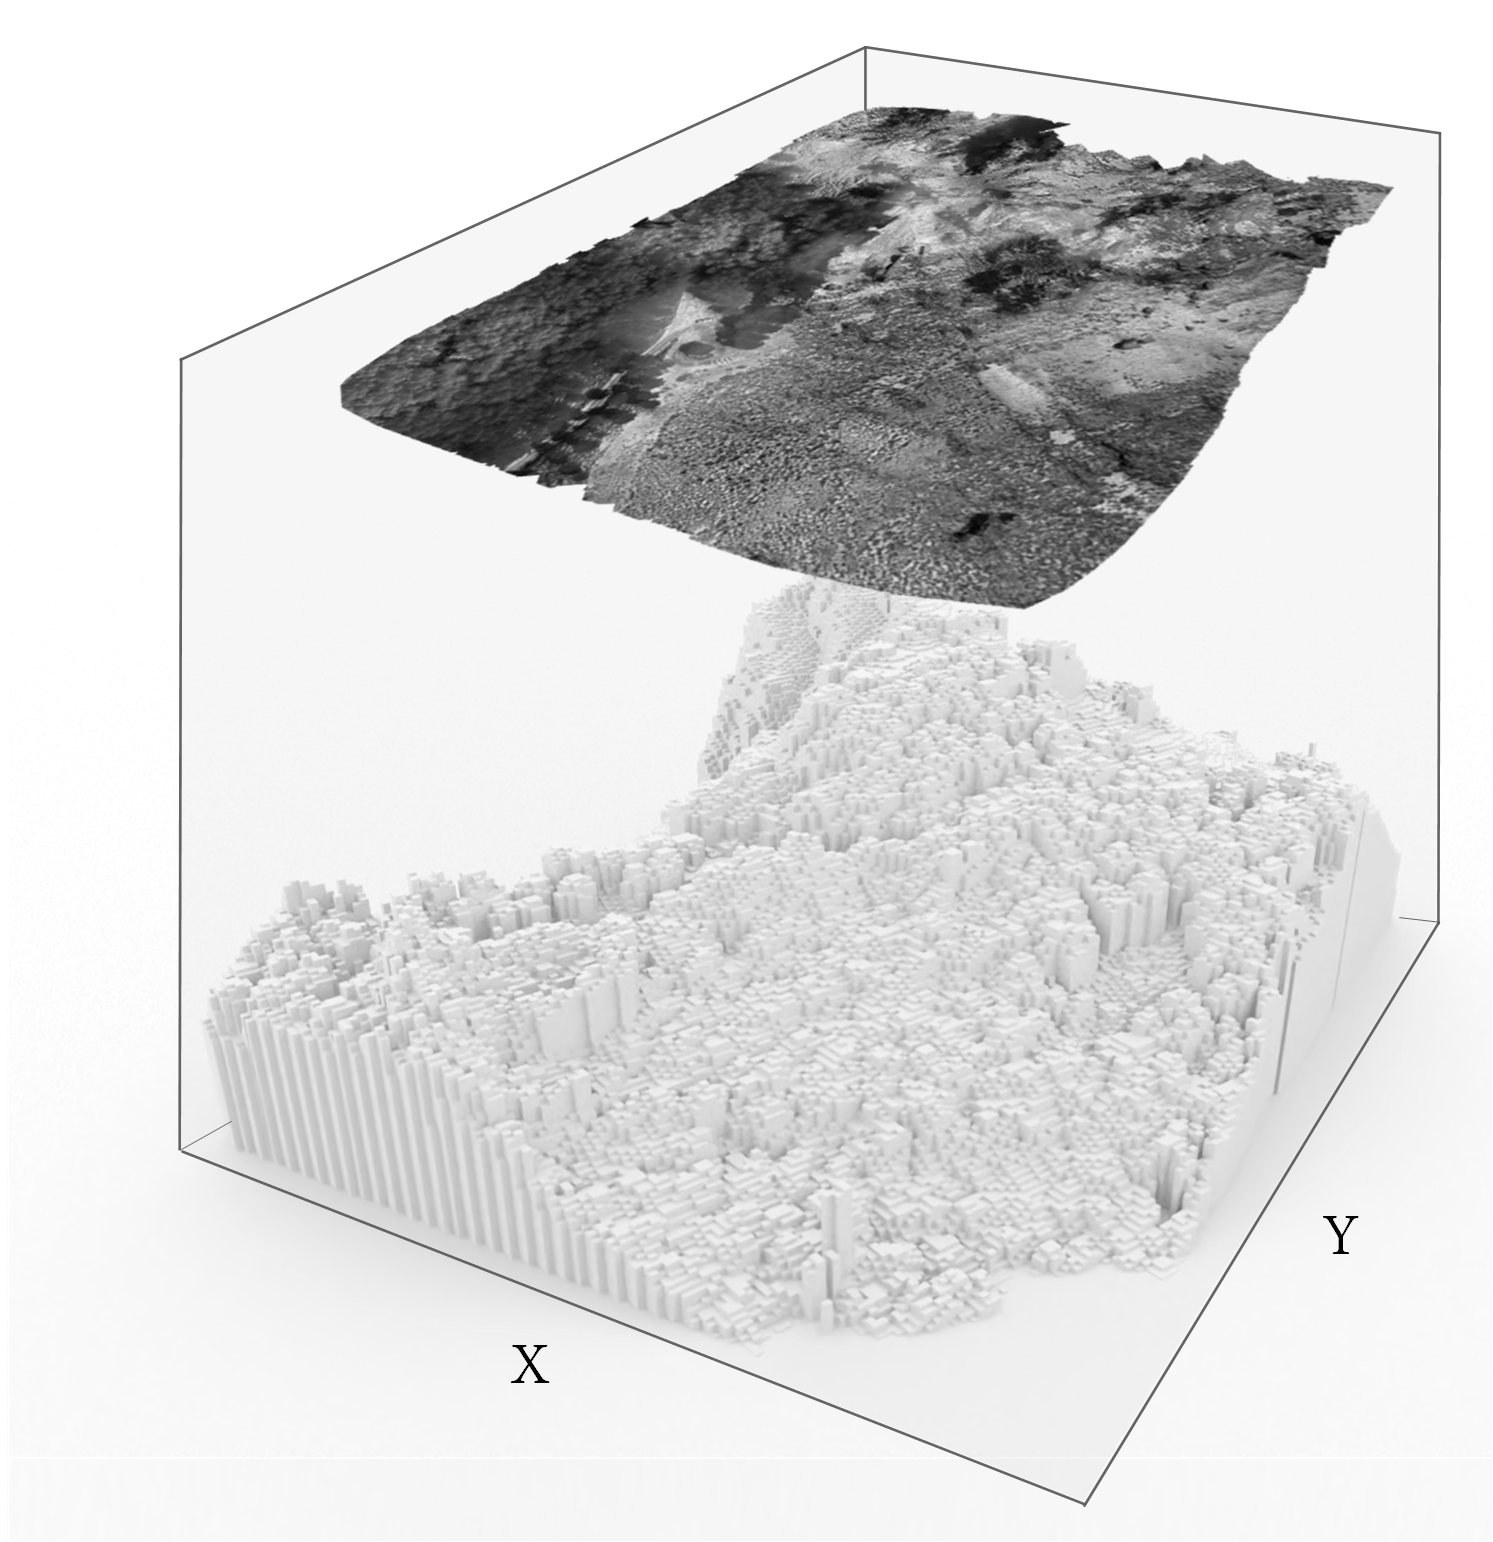
\includegraphics{figs/context/orthomosaic_projection.png}
	\caption{Projection of an orthomosaic over a 2.5D point cloud.}
	\label{fig:ortho_projection}
\end{marginfigure}
\acrshort{ir} 3D models can also be constructed by combining \acrshort{lidar} and visible point clouds with thermal maps in the same coordinate system (Figure \ref{fig:fusion_data_02}). Comba et al. \cite{comba_2d_2019} fused an \acrshort{rgb} point cloud with a thermal orthomosaic (Figure \ref{fig:ortho_projection}), whereas Adán et al. \cite{adan_towards_2020} combined \acrshort{lidar} results with 360-degree maps of \acrshort{ir} data. These studies generate a single thermal image with a limited resolution which is subsequently projected in a 3D model. The former approach obtains \acrshort{ir} heightfields (2.5D) \cite{juszczyk_wound_2021}, whereas the main drawback of the work of Adán et al. \cite{adan_towards_2020} is that some points lack \acrshort{ir} data as a result of foreground surfaces occluding background surfaces. This problem was mitigated by using a mobile scanning platform and joining multiple thermal point clouds using the platform odometry and the \acrshort{icp} algorithm. 

\begin{figure}[ht]
	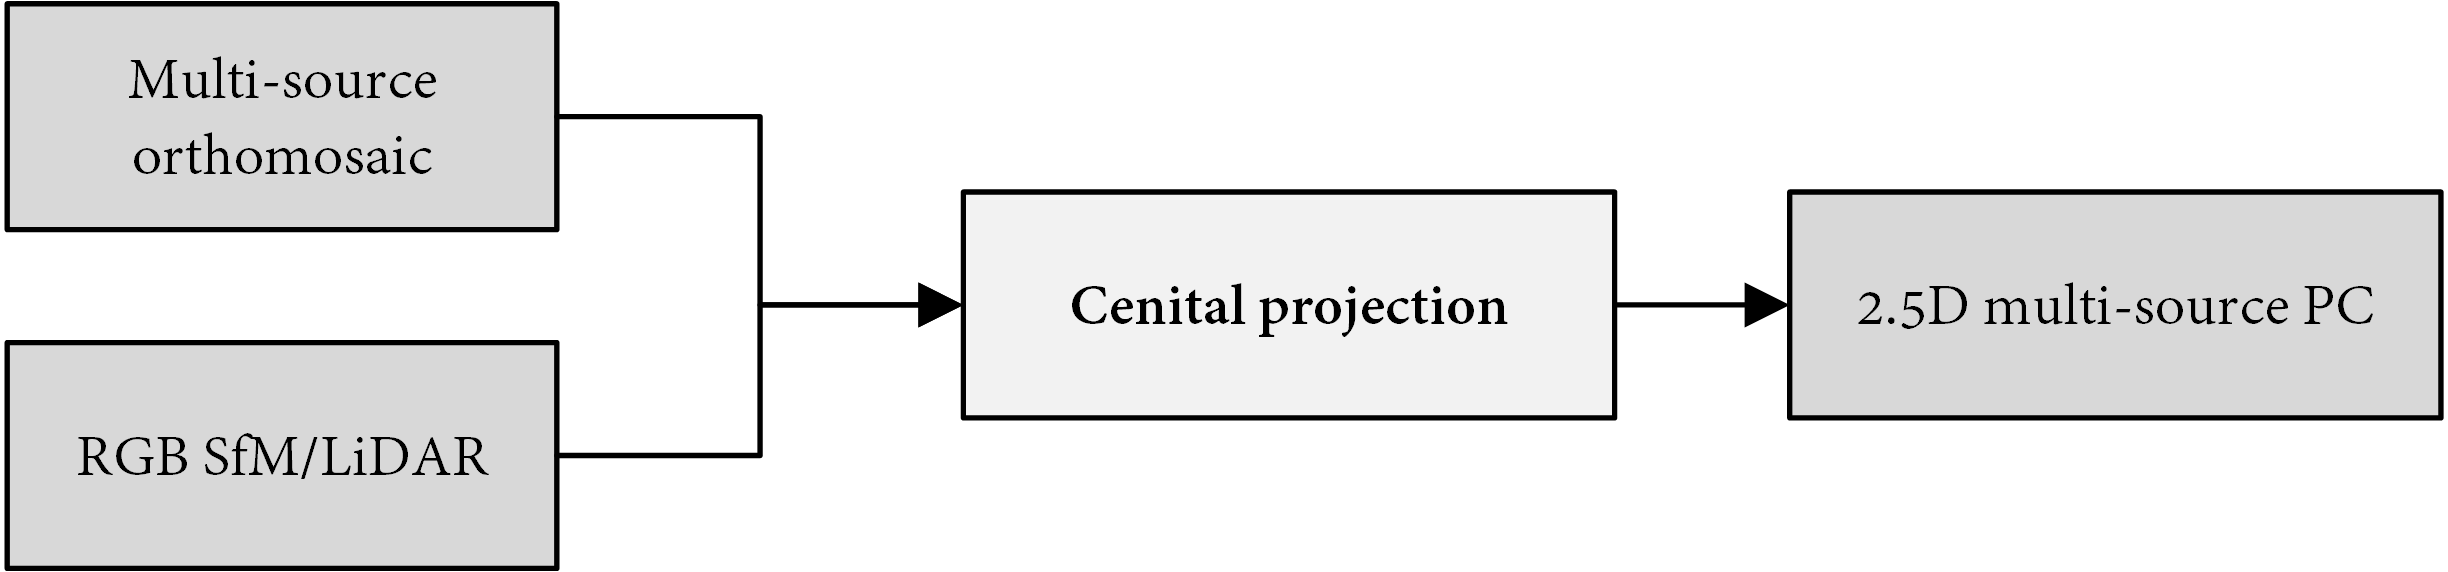
\includegraphics[width=\linewidth]{figs/context/fusion_02.png}
	\caption{2.5D point clouds are generated by projecting images from any data source into a baseline point cloud.}
    \label{fig:fusion_data_02}
\end{figure}

Finally, supervised procedures have also been proposed to match \acrshort{rgb} and thermal features. Huang et al. and Macher et al. \cite{huang_combining_2018, macher_combination_2019} used checkerboard images and relevant key points, such as building corners, to link features. Lafi et al. \cite{lafi_3d_2017} performed semi-automatic stitching of \acrshort{ir} images by marking relevant features, thus generating a panoramic image that was finally mapped to a 3D \acrshort{rgb} point cloud. However, semi-automatic registration is time-consuming and hard to apply over large datasets. Indeed, this procedure is more appropriate for datasets composed of a few images.

\subsection{Multispectral imaging}

The previous work focused on reconstructing 3D point clouds from multispectral imagery is coarsely split according to the use of satellite and \acrshort{uas} platforms. Traditionally, most of the previous work is based on satellite image mapping over 3D photogrammetric point clouds and \acrshort{lidar} models for monitoring the forest structure \cite{bolton_optimizing_2020, lechner_applications_2020}, multi-temporal observation of crops \cite{gadiraju_multimodal_2020, qadeer_spatio-temporal_2021} and semantic segmentation of urban and natural scenarios \cite{ballouch_toward_2022, saralioglu_semantic_2020}. State-of-the-art reconstruction methods from satellite data typically generate elevation data. \acrshort{dsm}s can be efficiently obtained with automatic image matching from multiple images acquired in the same orbit \cite{gui_automated_2021, qin_critical_2019}. Another promising field is the generation of super-resolution satellite images obtained with \acrshort{dl} \cite{gomez_experimental_2022, stucker_resdepth_2022}. Consequently, the cited advances and modern high-resolution satellite sensors enable recovering 3D surfaces from multi-view satellite panchromatic images \cite{han_state_2020, rothermel_photometric_2020}. The resulting 3D point clouds can be directly fused with multispectral bands of satellite imagery. 

Multispectral images acquired from \acrshort{uas} platforms have lower resolution than the majority of \acrshort{rgb} images, and yet, it is higher than the resolution provided by most \acrshort{ir} sensors. Therefore, 3D multispectral point clouds can be directly generated with photogrammetry \cite{liu_registration_2018, zainuddin_3d_2019, shen_estimation_2019, villacres_construction_2022, comba_unsupervised_2018}. Recently, Jurado et al. \cite{jurado_multispectral_2020} proposed a novel pipeline to generate dense multispectral point clouds by mapping images on dense \acrshort{rgb} point clouds. Firstly, a sparse \acrshort{nir} point cloud was reconstructed and aligned with the \acrshort{rgb} point cloud. The rest of the cameras were following projected and multispectral data was assigned to 3D \acrshort{rgb} points using \acrshort{knn}. Other approaches are based on multispectral data projection over 3D point clouds from \acrshort{rgbd} sensors embedded on aerial and terrestrial platforms. Clamens et al. \cite{clamens_real-time_2021} implemented a method based on feature-based and corner-based registration of \acrshort{rgbd} and multispectral images.

The integration of \acrshort{lidar} and multispectral sensors is another widely adopted approach. In recent years, the proliferation of lightweight \acrshort{lidar} sensors enables fusing data from a multispectral camera and \acrshort{lidar} sensor coupled to a \acrshort{uas}. Both sensors have usually the same \acrshort{gps} and \acrshort{imu} feed to avoid inconsistencies in the recorded time and space. Data fusion can be carried out by back-projecting data, i.e., rendering \acrshort{lidar} results from the optical camera’s perspective in order to correlate pixels and returns \cite{valbuena_integrating_2014}. Then, the pixel attributes are fetched and the \acrshort{lidar} returns are shaded. This projection is developed considering the optical sensor system (internal parameters) and the platform's position and bearing (external parameters). Sankey et al. \cite{sankey_quantifying_2021} proposed a novel methodology for \acrshort{uas}-based multispectral, hyperspectral and \acrshort{lidar} data fusion in shrub-encroached desert grassland. However, this study was based on a comparison between 2D multispectral and hyperspectral orthomosaics generated by Pix4Dmapper and SpectralView software, respectively. Gu et al. \cite{gu_uav-based_2020} integrated multispectral and \acrshort{lidar} sensors in a single system that simultaneously collected data. 

Photogrammetry can also help to generate orthomosaics of multispectral imagery, which can be later projected into \acrshort{rgb} point clouds \cite{comba_unsupervised_2018}. This procedure involves an orthogonal projection of multispectral orthomosaics to obtain 2.5D point clouds (see Figure \ref{fig:ortho_projection}). The main shortcomings of this approach are the geometric and radiometric inaccuracies obtained after computing an orthomosaic.

\subsection{Hyperspectral imaging}

The challenges of fusing \acrshort{hsi} and 3D models arise due to both data dimensionality and the required storage capacity. 3D reconstructions are easier to achieve with single-snapshot sensors since they can be generated using photogrammetry. However, push broom sensors pose several challenges due to the geometrical inaccuracies and the stitching of multiple swaths. This was already addressed in the fusion of 2D hyperspectral swaths, and it represents one of the first steps before fusing them with photogrammetric point clouds. 

The reconstruction of 3D hyperspectral point clouds has been previously achieved by fusing \acrshort{lidar} and \acrshort{hsi} \cite{lin_detection_2019, sankey_uav_2018}. Otherwise, it has been mainly addressed in close-range applications. For instance, Zia et al. \cite{zia_3d_2015} developed a method that applies \acrshort{sfm} to images from every collected wavelength and then, the wavelength-wise reconstructions were aligned. Kim et al. \cite{kim_3d_2012} described a system prototype composed of a laser sensor and a hyperspectral imager to characterize solid objects. Behmann et al. \cite{behmann_calibration_2015} proposed a method to generate 3D models from push broom sensors in close-range observations. This work used a polynomial transformation to describe the non-linear effects occurring in plant phenotyping, considering not only the linear model of the push broom sensors but also other distortion factors. The fusion of \acrshort{hsi} with models from laser scanners has also been addressed \cite{behmann_generation_2016}. Liu et al. \cite{liu_hyperspectral_2020} published an in-depth review of \acrshort{hsi} and 3D technologies for plant phenotyping by revising literature ranging from close-range applications to remote sensing. 

However, methodologies operating over measurements collected in the laboratory have a more controlled setup and stability in the sensor orientation. In contrast, these conditions are not guaranteed in outdoor scenarios with constantly changing conditions. For instance, the wind induces changes on the sensor and monitored scenes \cite{kalisperakis_leaf_2015}. Other works were capable of merging hyperspectral data in 3D models generated from standard \acrshort{rgb} cameras or laser scanning, thus enabling 3D geological modelling \cite{nieto_3d_2010} and 3D mapping of underwater environments \cite{ferrera_hyperspectral_2021}. 

Despite small-sized \acrshort{uas} enabling data acquisition with higher spatiotemporal resolution \cite{padua_uas_2017}, the integration of hyperspectral sensors is restricted due to payload capacity and flight autonomy \cite{bruning_approaches_2020}. These conditions harden their applicability to the monitoring of small-scale areas and research work. Even so, 3D hyperspectral modelling from \acrshort{uas} platforms is a recent technology that has become available to small-sized \acrshort{uas}s during the last decade \cite{nevalainen_individual_2017}. Some approaches use non-imager spectrometers in \acrshort{uas} platforms along with an \acrshort{rgb} sensor to accurately display the acquired spectral signatures over 3D information and orthomosaics acquired with \acrshort{rgb} data and photogrammetry \cite{garzonio_surface_2017}. For instance, Astor et al. \cite{astor_vegetable_2020} combined \acrshort{uas}-based \acrshort{rgb} data and ground-based \acrshort{hsi} for biomass estimation in different vegetable crops.

\acrshort{hsi} missions collect data by scanning and therefore, only a few perspectives of the area of interest are acquired in the flight direction, thus hardening the reconstruction of 3D scenarios. There is a void of methods accounting for this spatial heterogeneity to correctly merge hyperspectral data from push broom sensors into 3D models. With this approach, it would be possible to have a seamless data fusion integration that would lead to a very high spatial and spectral resolution. It can be expected that in the near future, \acrshort{uas}-based hyperspectral sensors will be capable of acquiring data in other parts of the \acrshort{em} spectrum, such as \acrshort{swir}, and even support on-board real-time processing \cite{horstrand_uav_2019, saari_visible_2017}.

\section{Simulation of Remote Sensing data}

Remote sensing imagers were conceived as mapping tools for generating products that help in the modelling and understanding of Earth's processes. However, the uprising combination of Remote sensing and \acrshort{ai} requires large datasets that enable trainable models to seek patterns in various scene perception tasks such as semantic segmentation, instance segmentation and classification applied over indoor and outdoor sceneries. Nonetheless, publicly available datasets may not suffix specific application requirements in terms of data density, attributes, kinds of scenes, recording platforms, etc. Amongst the most common examples of this is the advent of autonomous driving, which required large and variate annotated \acrshort{lidar} datasets to achieve safe systems capable of working under most conditions. Similarly, the semantic segmentation of \acrshort{lidar} has drawn the attention of both industry and academia. Multiple real-world \acrshort{lidar} datasets have been published over the last years, most of them focused on urban scenarios recorded with static or mobile platforms. Still, some of them are not labelled, do not include trajectories or \acrshort{gps}/\acrshort{imu} data, lack supplementary cameras, etc. \cite{cai_survey_2022}. 

The generation of synthetic \acrshort{lidar} data is among the most frequent computerized processes. However, the synthetic modelling of images has also been gaining interest \cite{yi_cycle_2023, ozkanoglu_infragan_2022}, especially for those spectral ranges which are not as widespread in publicly available datasets. For example, this is the case of infrared imagery, which is also influenced by the increasing demand for autonomous systems. Unlike visible cameras, infrared cameras do not rely on external light sources and therefore are appropriate for making autonomous systems understand their context even at night and in adverse daylight conditions. Among its applications, infrared may be required for reading traffic signals, wildlife and human detection and object tracking \cite{vollmer_infrared_2017}.  

\subsection{Motivation of synthetic \acrshort{lidar} simulation}

\acrshort{lidar} sensors are expensive imagers that require mobile or static platforms to generate a point cloud of the target scenario. To this end, one or multiple scans can be collected and joined by means of overlapping features. On the other hand, \acrshort{lidar} simulators are much more cost- and time-efficient once the emulation challenge has been resolved, which is neither trivial nor efficient to address. Simulating data avoids carrying out fieldwork to generate massive datasets and enables optimizing the planning of real \acrshort{lidar} scans \cite{mohan_robust_2019, li_3d_2022}. Instead of performing scans on real-world scenarios, simulations are performed over synthetic models that can be annotated with any \acrshort{lod}. Thus, these can feed the resulting point cloud with ground-truth data concerning a large number of attributes, from normal vectors to semantic annotations. 

There are multiple applications of \acrshort{lidar} simulations, along with their corresponding research niches. From a hardware perspective, some simulators are focused on the design, validation and calibration of \acrshort{lidar} sensors \cite{lee_validation_2020}. Their objective is to detect and reduce errors in the scanning, both systematic and random. There are also simulators focused on the optimization of scanning processes \cite{iqbal_simulation_2020, westling_simtreels_2020}, such as the integration of \acrshort{lidar} data into enhanced and synthetic vision systems \cite{peinecke_lidar_2008}. From a software perspective, one of the most popular research topics is autonomous driving \cite{fang_augmented_2020, li_deep_2020} and navigation \cite{manivasagam_lidarsim_2020}. Most of these methods, especially those based on \acrshort{dl}, benefit significantly from synthetic data. 

Beyond generic research purposes, including teaching and learning, there are systems aimed at the custom configuration of the simulated sensors, including their mounting platform and setup. These simulators typically allow the user to fine-tune all the parameters needed for a physically-based simulation of the laser beams and the interaction with the virtual environment, where photon mapping, Monte Carlo simulation, and full \acrshort{lidar} waveform generation are their core foundations \cite{yun_simulation_2019, chen_ole_2020, zohdi_rapid_2020}. These frameworks can simulate multiple scattering of the laser beams, taking into account their propagation through wind-driven rough air-water interface \cite{chen_ole_2020}, or vegetation \cite{yun_simulation_2019, westling_simtreels_2020}. There also exist commercial and open-source software such as LGSVL (LG) \cite{lg_electronics_rd_lab_lgsvl_2021}, Simcenter (Siemens Software) \cite{siemens_simcenter_2021}, and CARLA \cite{dosovitskiy_carla_2017} for generating autonomous driving datasets.

\subsection{Public \acrshort{lidar} datasets}

The vast majority of \acrshort{lidar} datasets focus on autonomous driving and perception tasks such as classification, semantic segmentation, instance segmentation and tracking of mobile objects \cite{chen_automatic_2022}, using geometrical \cite{behley_towards_2021} and intensity information \cite{tan_toronto-3d_2020}. Most of them record metropolitan environments from a mobile vehicle coupled with a \acrshort{lidar}, along with visible and infrared cameras in a few case studies \cite{choi_kaist_2018}. On the other hand, aerial \acrshort{lidar} datasets covering large portions of the Earth's surface are frequently published by governmental institutions at land inventorying portals. Since these are intended to cover large areas, they are acquired from mid-altitude platforms with a density of a few points per squared meter (up to two points according to the United States Geological Survey \cite{us_geological_survey_lidar_2012} and 0.5 points for the Spanish National Plan of Land Observation \cite{instituto_geografico_de_informacion_geografica_pnoa_nodate}). More recently, despite not being frequent, large and denser aerial \acrshort{lidar} datasets have also been published \cite{varney_dales_2020}. 
\begin{marginfigure}[.0cm]
	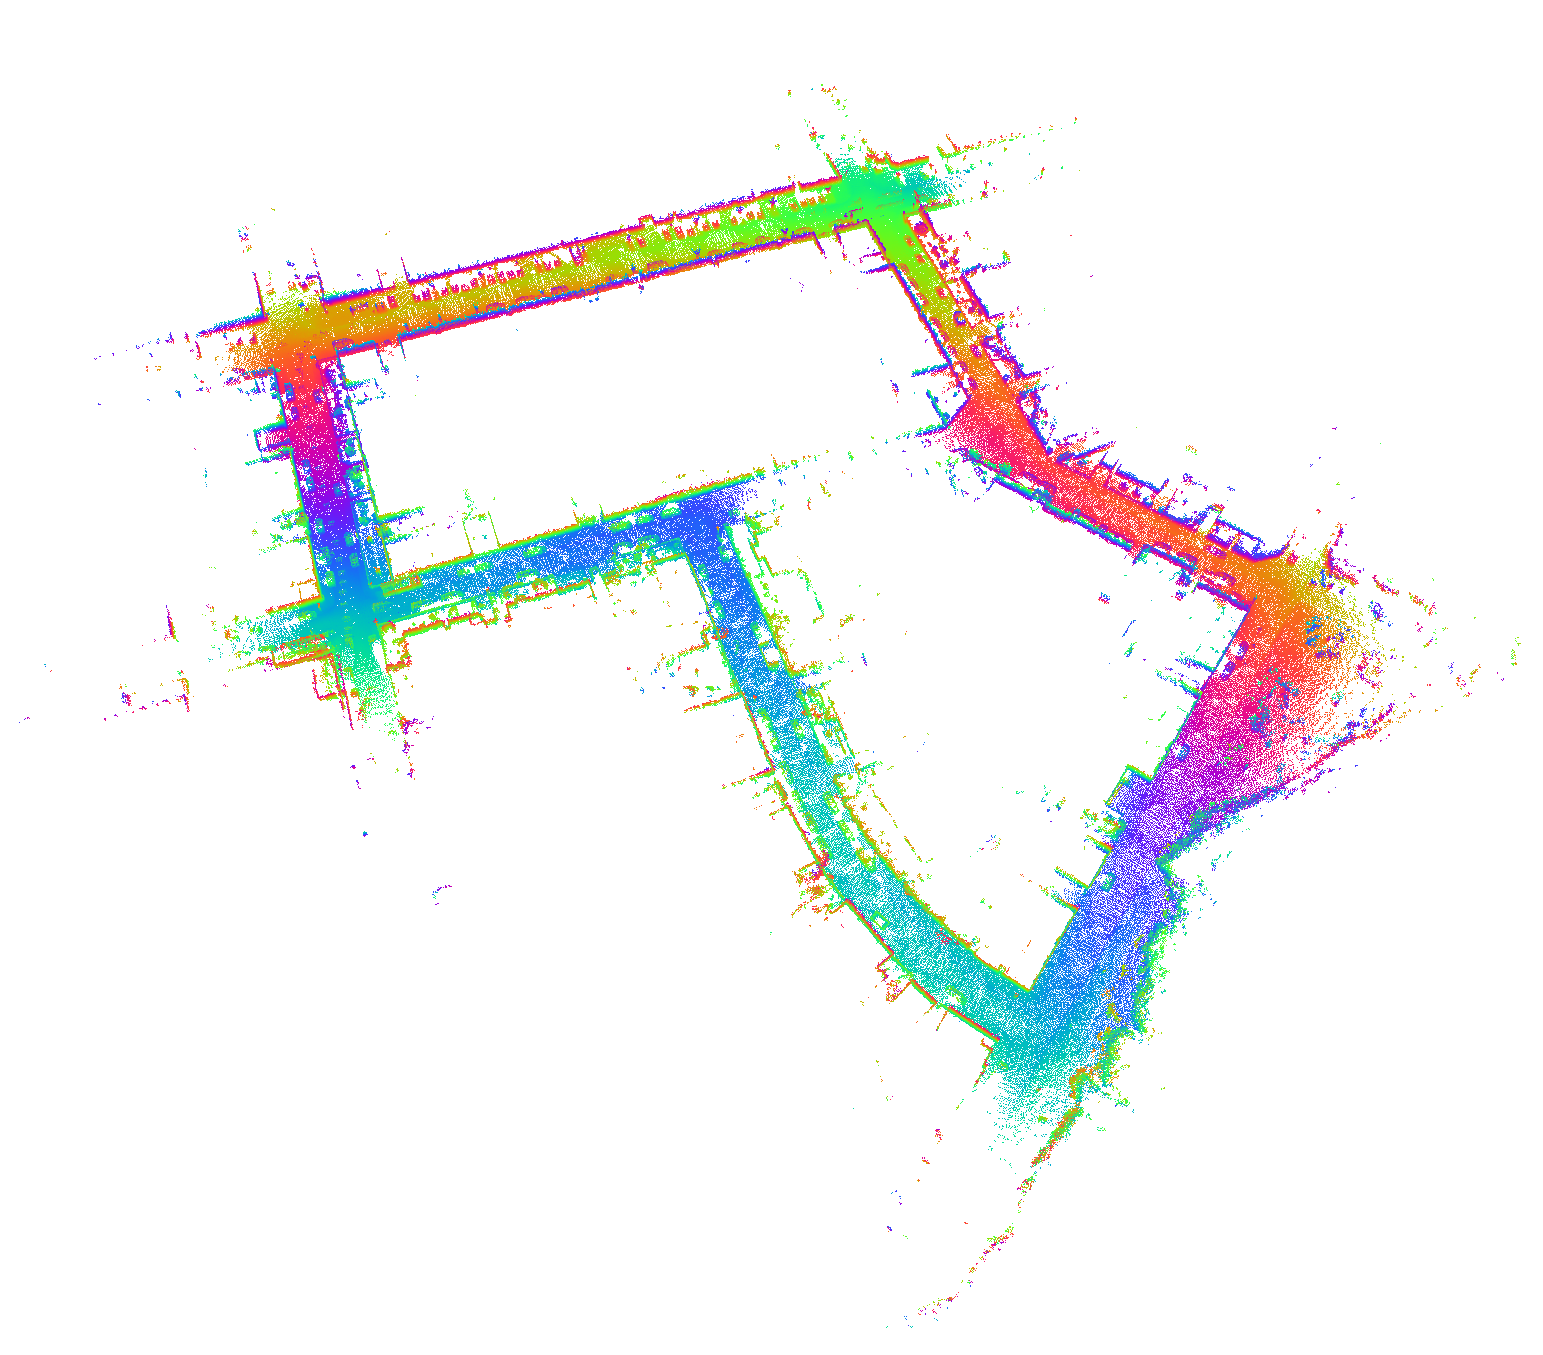
\includegraphics{figs/context/kitty_scan.png}
	\caption{Example of a metropolitan \acrshort{lidar} point cloud in the SemanticKITTI dataset \cite{behley_towards_2021}, composed of a sequence of scans recorded from a vehicle coupled with a Velodyne \acrshort{lidar}.}
	\label{fig:kitty_scan}
\end{marginfigure}

Both kinds of datasets, terrestrial and aerial, are required to be annotated to be applied to \acrshort{dl}. Previously revised datasets are recorded by real sensors, and therefore, their classification must be performed manually \cite{behley_towards_2021, pan_semanticposs_2020, tan_toronto-3d_2020} or automatized with networks trained with very limited data \cite{wu_squeezesegv2_2019}. Manual labelling induces errors, but another shortcoming is the lack of detail. For example, these are some real datasets and the number of different semantic labels: SemanticKITTI (25) \cite{behley_towards_2021}, nuScenes (23) \cite{caesar_nuscenes_2020}, SemanticPOSS (14) \cite{pan_semanticposs_2020}, Toronto-3D (8) \cite{tan_toronto-3d_2020} and Semantic3D (8) \cite{hackel_semantic3d_2017}. More recently, \acrshort{lidar} datasets have been released together with video and audio data \cite{piadyk_streetaware_2023} (see Figure \ref{fig:lidar_audio_video}). A more complete compilation of open-source real \acrshort{lidar} datasets can be found in \cite{cai_survey_2022}. 

\begin{figure}[ht]
	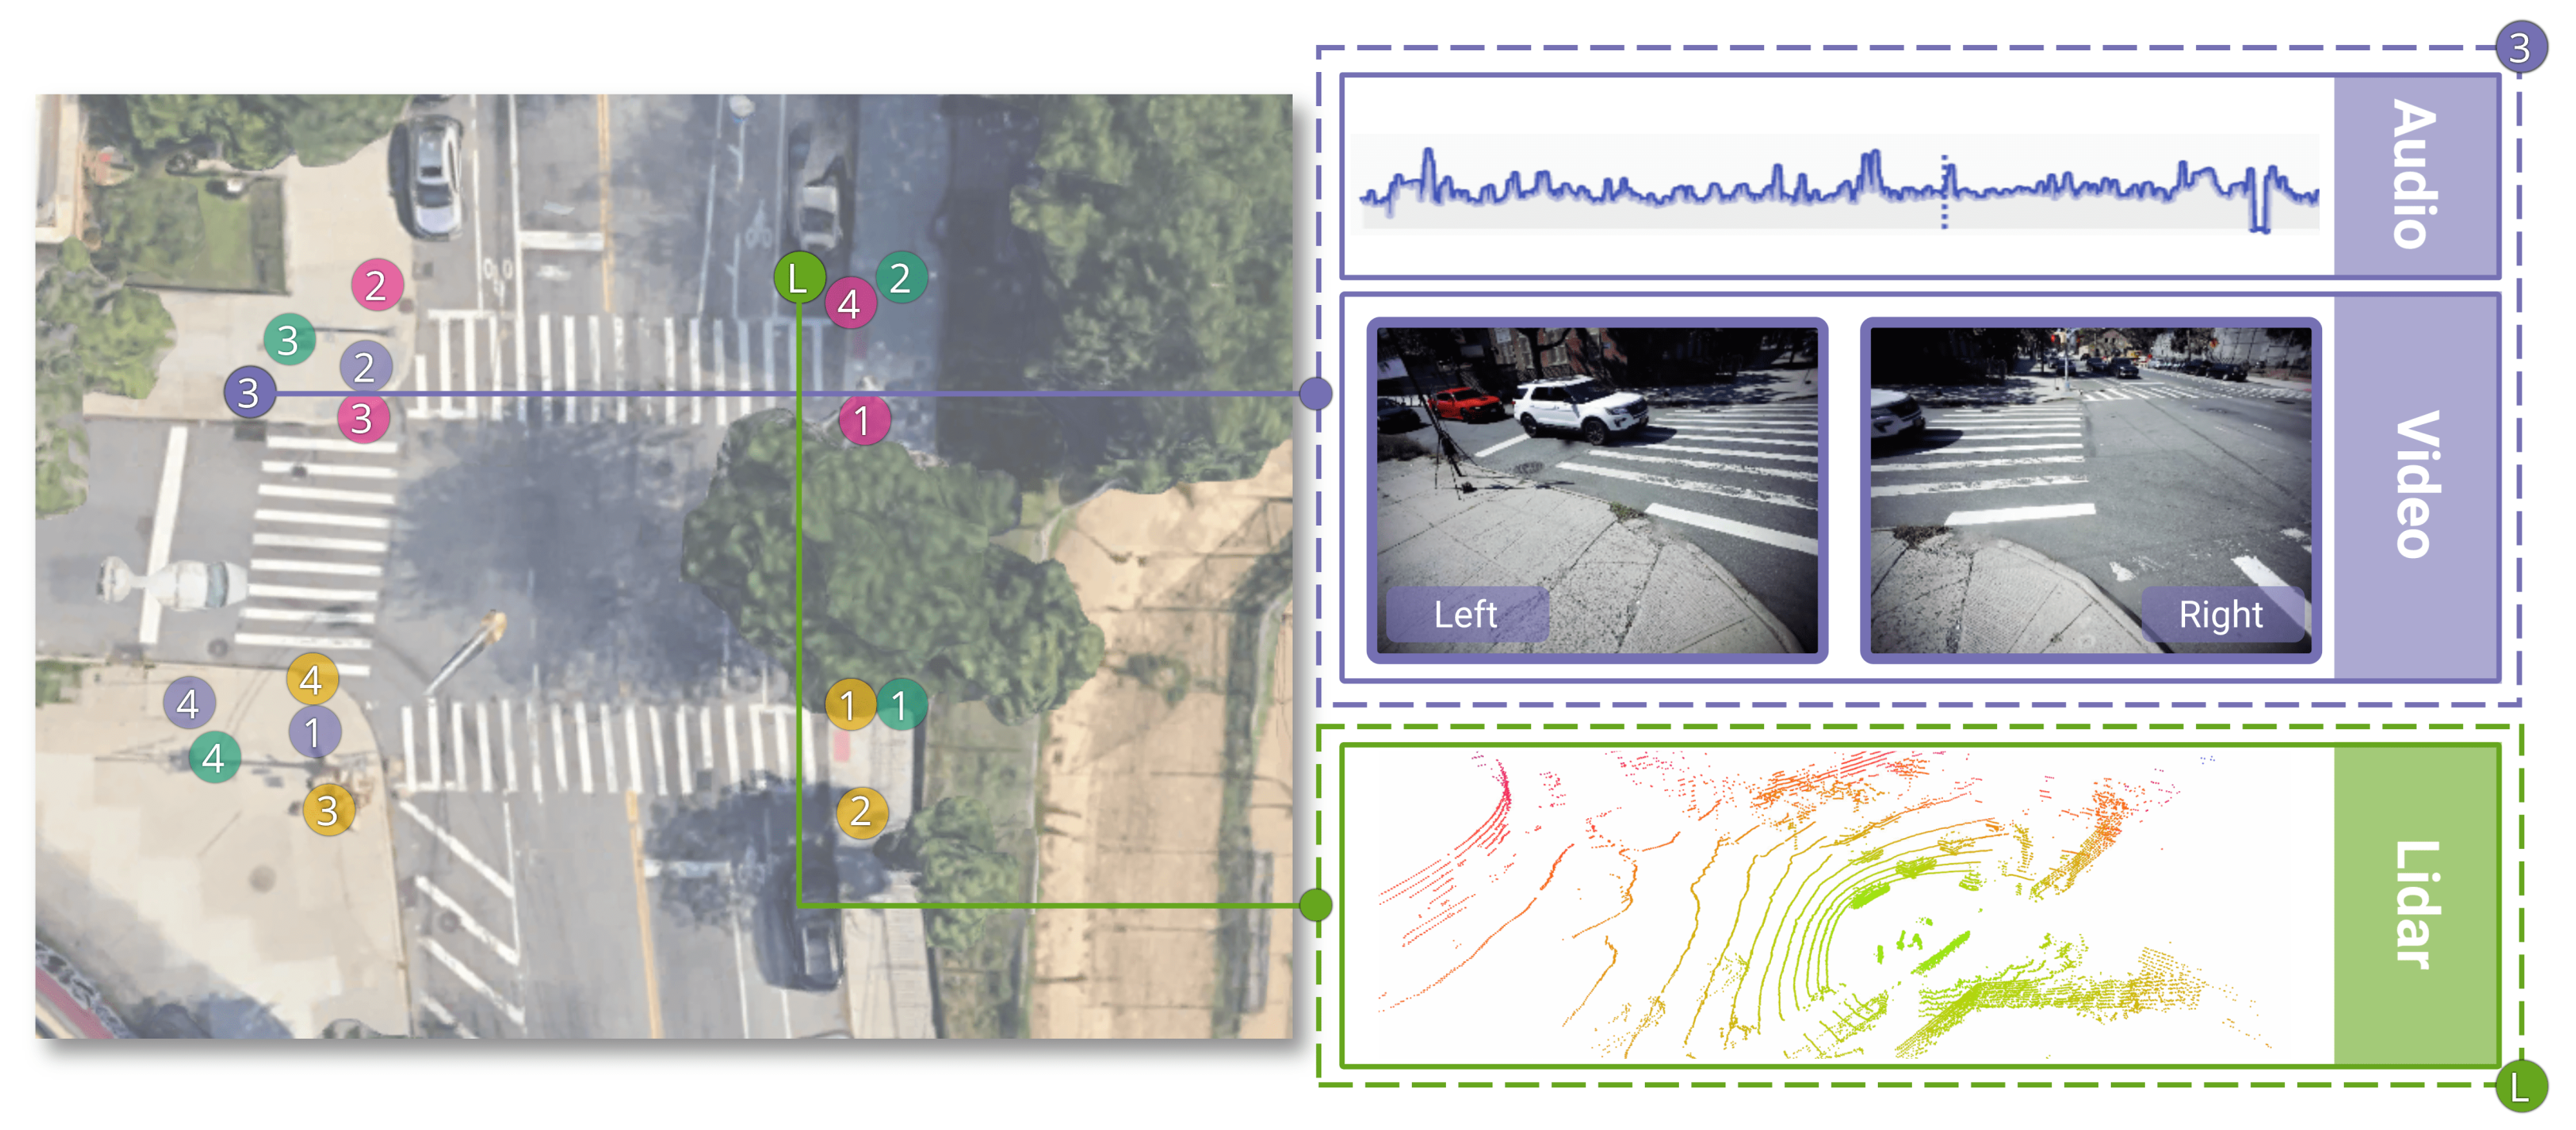
\includegraphics[width=\linewidth]{figs/context/lidar_dataset_audio_video.png}
	\caption{Overview of the data collection proposed by Piadyk et al. \cite{piadyk_streetaware_2023}, where \acrshort{lidar} is captured along with audio and video feed. }
    \label{fig:lidar_audio_video}
\end{figure}

\subsection{\acrshort{lidar} simulation}

The early \acrshort{lidar} simulators produced graphically feasible \acrshort{lidar} point clouds \cite{gschwandtner_blensor_2011} by emulating the sensor's \acrshort{fov}, occlusion and beam divergence. \acrshort{lidar} returns can be solved with ray-casting \cite{ahn_real-time_2020, zhao_method_2021, bechtold_helios_2016} in annotated environments. Remark that ray-casting implies solving impacts of laser beams in the followed path, frequently ranging from one to five returns, whereas ray-tracing refers to emulating light interaction among surrounding surfaces. The latter represents a physically-based simulation that requires an enormous computation effort and therefore is not yet practical \cite{ahn_real-time_2020}. In recent years, \acrshort{lidar} simulators have addressed the realistic simulation of geometry returns, the impact of surface properties as well as other environmental conditions. 

Some of the aspects of what is expected from physically-based results have been simulated by including a wide number of errors and limitations. First, Xhao et al. \cite{zhao_method_2021} modelled atmospheric effects such as rain, snow and fog by including signal attenuation and noise. Haider et al. \cite{haider_development_2022} have recently modelled the signal processing of \acrshort{lidar} as well as scan patterns to emulate optical losses and defects. Among the cited features, signal attenuation \cite{dosovitskiy_carla_2017, bechtold_helios_2016, hanke_generation_2017}, beam divergence \cite{zhao_method_2021, bechtold_helios_2016, hanke_generation_2017, haider_development_2022} and drop-off in intensity \cite{ahn_real-time_2020} are frequent in the literature. Very few address multiple returns \cite{winiwarter_virtual_2022} despite simulating beam divergence. Other not-that-frequent errors are mirror reflection \cite{ullrich_advances_2019}, motion distortion \cite{chen_analysis_2022}, non-uniform density and distortion of point attributes (colour, intensity, etc.), either as a result of an inappropriate setup \cite{dimitrov_segmentation_2015}, or systematic and random errors \cite{isheil_systematic_2011, fan_error_2015, pandzic_error_2017}. Random errors depend on aspects like the signal-to-noise ratio of the received signal, the accuracy of the electronics (including again the \acrshort{imu} and the \acrshort{gps}), the divergence of the laser beams (jittering) and their wavelength, as well as the reflectivity of the objects. Instead of physically emulating these features, previous work has deviated ideal synthetic \acrshort{lidar} point clouds with \acrshort{dl} \cite{manivasagam_lidarsim_2020, xiao_synlidar_2021, guillard_learning_2022}. The leveraging of real \acrshort{lidar} and synthetic point clouds has also been investigated by mixing scanned urban scenarios and synthetic objects \cite{manivasagam_lidarsim_2020}. Nonetheless, annotation and ground-truth shortcoming remains when leveraging both kinds of data.

\begin{marginfigure}[.0cm]
	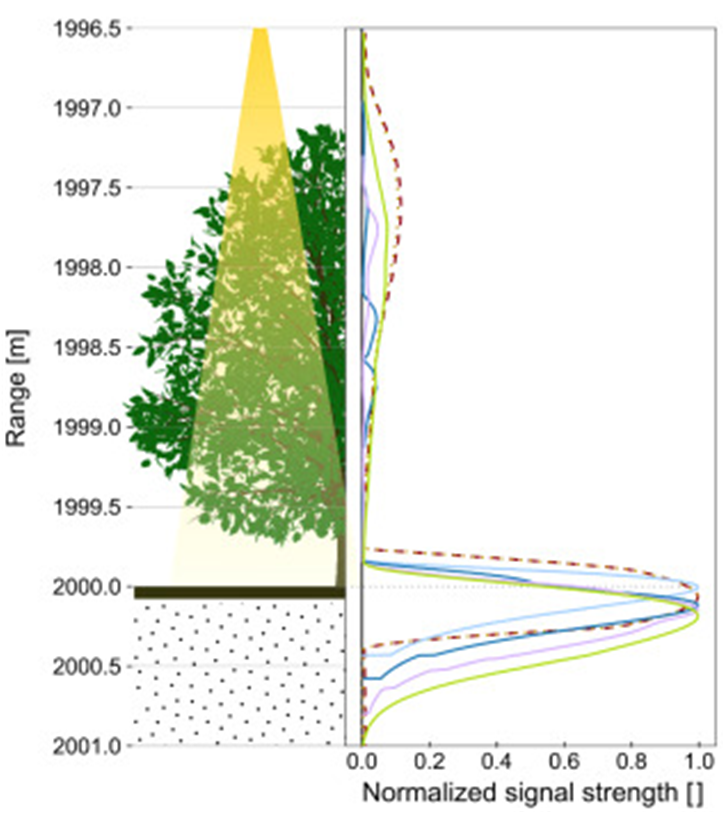
\includegraphics{figs/context/waveform_lidar.png}
	\caption{Simulation of a full-waveform \acrshort{lidar} traversing a tree \cite{winiwarter_virtual_2022}.}
	\label{fig:full_waveform_lidar}
\end{marginfigure}
Most of the revised simulators are focused on Terrestrial Laser Scanning (\acrshort{tls}), while Airborne Laser Scanning (\acrshort{als}) has barely been addressed \cite{winiwarter_virtual_2022}. Westling et al. \cite{westling_simtreels_2020} included \acrshort{als} as an unrealistic extension of \acrshort{tls}. Bechtold and Höfle \cite{bechtold_helios_2016} simulated \acrshort{als} with different scanning geometries (Figure \ref{fig:scan_geometries_lidar}), which is one of the main challenges of \acrshort{als}. More recently, Winiwater et al. \cite{winiwarter_virtual_2022} extended the work of Bechtold and Höfle to incorporate full-waveform \acrshort{lidar} (Figure \ref{fig:full_waveform_lidar}. Rather than capturing discrete returns, this kind of sensor returns the intensity recorded over a path. For instance, it helps to measure the amount of vegetation at different altitudes for forest inventory. One of the main inconveniences of this solution, published under the name of HELIOS++, is that input environments are simplified by means of voxels and therefore lose part of the scene details.

\begin{figure}[ht]
	\includegraphics[width=\linewidth]{figs/context/scan_geometries_lidar.png}
	\caption{Overview of different scanning geometries from the HELIOS++ simulator: a) rotating mirror, b) oscillating mirror, c) fibre-optic line scanner, d) slanted rotating mirror (Palmer scanner), and e) Risley prisms (i.e., Livox scanner). }
    \label{fig:scan_geometries_lidar}
\end{figure}

On the other hand, the modelling of materials typically estimates the reflectance using phenomenological \acrshort{brdf}s such as Oren-Nayar, Lambertian and Blinn-Phong \cite{chen_analysis_2022}, regardless of the sensor wavelength \cite{chen_analysis_2022, gschwandtner_blensor_2011, zohdi_rapid_2020}. Other studies use diffuse, specular and transmissive properties acquired from commercial frameworks, such as CarMaker \cite{haider_development_2022}. Intensity has also been simulated using \acrshort{dl} with \acrshort{lidar} data represented as images instead of points \cite{vacek_learning_2022, xiao_synlidar_2021}. However, these networks are constrained to the variety of materials and lighting conditions in the training datasets. 

\subsection{Time efficiency}

Most studies do not evaluate the efficiency of the proposed solution, and \acrshort{dl} networks are constrained to the response time of the network. To the best of our knowledge, only Peinecke et al. \cite{peinecke_lidar_2008} have considered a \acrshort{gpu}-based simulation in \acrshort{opengl}. Also, the efficient semantic labelling and generation of synthetic environments have been poorly addressed, including the annotation of virtual scenes composed of \acrshort{cad} models. Another key factor is the precision of the synthetic scans: previous work has simulated \acrshort{lidar} scans using depth buffers \cite{su_simulation_2019, fang_augmented_2020, manivasagam_lidarsim_2020} with a limited resolution, frequently $2^8$ unless the target texture is composed of floating-point values. 

\section{Optimization of LiDAR scans in indoor environments}

\subsection{Motivation} 

\acrshort{lidar} is widespread in the construction industry for the tracking of building progress by enabling the acquisition of the environment geometry in a precise and highly detailed way. Instead of polygonal meshes, a discretized representation of buildings is given by point clouds. To achieve this goal, \acrshort{tls} is increasingly being used to collect large sets of building data \cite{pandzic_error_2017}. This technology can be applied to a wide range of applications, including building inspections \cite{shariq_revolutionising_2020}, monitoring of natural environments (landform dynamics \cite{guisado-pintado_3d_2019}, ecological resilience \cite{mitasova_geospatial_2010}, etc.), autonomous driving \cite{kuutti_survey_2021} or preservation of cultural heritage \cite{banfi_integration_2019, ham_phased_2020, andriasyan_point_2020}, among others. Besides terrestrial scanners, \acrshort{lidar} technology presents multiple variants according to their capabilities (range, spatial resolution and covering, etc.) and the platform from which they are operated (\acrshort{als}, \acrshort{tls}, \acrshort{mls}, \acrshort{bmmls}, etc.) \cite{poux_smart_2019, warchol_concept_2019}. 

Some of the main challenges of \acrshort{tls} in the surveying of 3D facilities are the occlusion and range limitations \cite{soudarissanane_optimizing_2012}. Consequently, appropriate planning of \acrshort{tls} scans is necessary in order to 1) minimize the number of different acquisition points, 2) generate a uniformly dense point cloud, and 3) reduce the occlusion from scene objects. These three objectives are equally influenced by the configuration and placement of the scanner. On the other hand, periodic scanning and monitoring of buildings are especially relevant for digitized representations, such as the widely known Building Information Modelling (\acrshort{bim}) \cite{macher_point_2017}. They encode characteristics of a building, including 3D design drawings, materials, costs and safety specifications \cite{patraucean_state_2015}, and provide an interface for the management of 4D applications. Together with \acrshort{tls}, it allows the monitoring of continuously evolving buildings to preserve cultural heritage, track its current state and maintain repair records \cite{rocha_scan--bim_2020, andriasyan_point_2020, moyano_bringing_2020, ham_phased_2020}. However, the monitoring of buildings over time is time-consuming, especially in dynamic environments. Also, \acrshort{tls} surveys generate multiple point clouds that need to be fused either by placing target marks \cite{gollob_comparison_2020} or by estimating the rigid transformation that minimizes the distance among overlapping point clouds. In order to speed up this acquisition task, the development of tools for the planning of \acrshort{tls} surveys plays a key role.

\subsection{Planning for Scanning}

The Planning for Scanning (\acrshort{p4s}) has previously been addressed using a wide range of environments and techniques. If the number of target locations is known, then the selection of an optimum set is also known as the NP-complete set-coverage problem \cite{li_probability_2021, mohamadi_efficient_2021, roostapour_pareto_2022}. Previous research can be categorized according to the input environment: model-based or non-model-based (discovered as being explored). The latter is mainly applied to robotic applications whose environment is unknown \cite{potthast_probabilistic_2014}. Otherwise, input scenarios are either defined as 2D or 3D models, with 2D representations being cross-sections of buildings \cite{giorgini_sensor-based_2019}. Solutions for 2D inputs present lower computational complexity and are frequently solved following an iterative selection of viewpoints (Next Best View; \acrshort{nbv}) or heuristic algorithms \cite{aryan_planning_2021}. The main drawback of these algorithms is that they do not consider the details underneath complex buildings. Instead, they are focused on 2D sketches composed of wall edges. 3D-based approaches are far more complex and guided by metrics that allow filtering and ordering spatial locations, as in Figure \ref{fig:planning_for_scanning_room}. Despite this, the exploration of 3D buildings is also approached with heuristics and \acrshort{nbv}. However, the high latency frequently leads to simplifications of the environment using voxelizations \cite{wakisaka_optimal_2019, rougeron_optimal_2022}, axis-aligned bounding boxes (\acrshort{aabb}) and object-oriented bounding boxes (\acrshort{oobb}) \cite{li_3d_2022}. A similar work to ours was published at the same time, also partly implemented in \acrshort{gpu} \cite{rougeron_optimal_2022}. However, the environment was voxelized and the number of optical locations was set by users, instead of being part of the optimization. On the other hand, Chen et al. \cite{chen_3d_2022} solved the \acrshort{p4s} optimization over 3D scanned façades using a Greedy algorithm. The weight of each location was estimated from a \acrshort{lidar} simulation. Finally, 2.5D models, such as \acrshort{dsm}s, have also been investigated in a similar way to 2D environments \cite{starek_viewshed_2020}.

\begin{figure}[ht]
	\includegraphics[width=\linewidth]{figs/context/planning_for_scanning.png}
	\caption{Example of 3D model for experimentation of \acrshort{p4s}. The main scene has another inner room which some gaps which serve to stress the planning for scanning algorithm. It helps to show how algorithms perform in terms of \acrshort{lod}, \acrshort{loa} and \acrshort{loc}.}
    \label{fig:planning_for_scanning_room}
\end{figure}

\subsection{Metaheuristics}

Heuristics are the most frequent solver in \acrshort{p4s}. Although they do not provide optimal solutions, they are proven good enough to cover environments with minimum scanning locations. Among heuristics, the Greedy algorithm has been extensively investigated \cite{zhang_rapid_2016, giorgini_sensor-based_2019, heidari_mozaffar_optimal_2016}, followed by Simulated Annealing (\acrshort{sa}) \cite{chen_indoor_2018}, Genetic Algorithms (\acrshort{ga}) \cite{jia_comparison_2017}, Particle Swarm Optimization \cite{jia_comparison_2017} and Integer Programming \cite{wakisaka_optimal_2019}. Greedy algorithms are based on the iterative selection of locations, according to an objective function. Other Greedy variations weight the locations using a visibility score \cite{jia_comparison_2017}, while others are followed by \acrshort{sa} \cite{latimer_sensor_2004}, or optimized with Divide and Conquer (\acrshort{d&c}) \cite{zhang_rapid_2016}. Instead of providing an automatic pipeline, \cite{ahn_interactive_2016} proposed an interactive semi-automatic system.

\begin{figure}[ht]
	\includegraphics[width=\linewidth]{figs/context/genetic_algorithm.png}
	\caption{Overview of the iterative process and data encoding in a Genetic Algorithm (\acrshort{ga}). }
    \label{fig:genetic_algorithm}
\end{figure}

Heuristic solvers are guided by objective functions measuring the quality of achieved solutions. To evaluate this, four metrics are frequently used in previous work \cite{li_3d_2022, aryan_planning_2021}: Level of Detail (\acrshort{lod}), Level of Accuracy (\acrshort{loa}), Level of Overlap (\acrshort{loo}) and Level of Coverage (\acrshort{loc}). \acrshort{lod} refers to the point cloud resolution, \acrshort{loa} measures the quality of \acrshort{lidar} returns, as higher distances and angles deteriorate the quality of the measurements \cite{ aryan_planning_2021}, \acrshort{loo} refers to the overlapping area among point clouds so that \acrshort{tls} scans can be joined with rigid transformation estimations (e.g., \acrshort{icp}), and \acrshort{loc} refers to the number of polygons reached by scans. Thus, the optimization is very influenced by the \acrshort{lidar} range and incidence angles. 

\begin{marginfigure}[3.0cm]
	\includegraphics{figs/context/uav_path_planning.png}
	\caption{Path planning of a fixed-wing military \acrshort{uas} with the objective of minimizing flight altitude and fuel consumption.}
	\label{fig:path_planning_uav}
\end{marginfigure}
Research on heuristics in 3D is also frequent in the literature, though they are mostly linked to path planning \cite{pehlivanoglu_enhanced_2021, roberge_parallel_2021} (see Figure \ref{fig:path_planning_uav}) and the selection of subsets \cite{pehlivanoglu_enhanced_2021}. However, the number of scans needed to meet the required quality is unknown in a non-finite 3D space. The set of possible solutions can be narrowed either by selecting random locations \cite{chen_indoor_2018} or sampling the environment as a 2D grid \cite{starek_viewshed_2020, giorgini_sensor-based_2019, jia_comparison_2017}. For uniform subdivisions, the level of detail of the tessellation is a key factor with regard to response time. Coarse subdivisions present lower latency, though they are prone to yield far from optimal solutions. Starek et al. \cite{starek_viewshed_2020} enhanced initial locations by applying minor translations while assessing their quality through an objective function, whereas Soudarissanane and Lindenbergh \cite{soudarissanane_optimizing_2012} improved the sampling by increasing the grid subdivisions, at the expense of higher response time. For 3D locations, Starek et al. \cite{starek_viewshed_2020} described a \acrshort{sa} procedure to translate uniformly sampled points into surrounding locations that improve the covering metric. Kim et al. \cite{kim_placement_2020} tried to find the optimal \acrshort{lidar} position over an autonomous vehicle using Genetic Algorithms (\acrshort{ga}). For that purpose, the specifications of commercial \acrshort{lidar}s were used to compute the occupancy grid, defined as a discretized $360^\circ$ map represented by several views acquiring the coverage region and dead zones. Beyond theoretical/simulation approaches, multiple studies focus on evaluating the set-up of several sensors, concerning height, angles and location in autonomous driving \cite{pereira_self_2016, veronese_accurate_2018}. 

Once locations are locally optimized, they are processed as a classic set-coverage problem \cite{soudarissanane_optimizing_2012}. Recent research has solved this with \acrshort{ga}, using different operators and configurations \cite{wang_solving_2018, roostapour_pareto_2022, mohamadi_efficient_2021}. Local searches \cite{li_probability_2021} and other nature-inspired heuristics \cite{islambouli_optimized_2019} are also reviewed. Despite heuristics being allowed to solve hard problems with optimal or nearly optimal solutions, these are not efficient in most cases. Previous studies regarding \acrshort{p4s} required hours, even days, to determine the optimal scanning configuration in 3D environments. Even 2D-based approaches are time-consuming \cite{giorgini_sensor-based_2019} if they are implemented in a sequential manner. Thus, multi-core and \acrshort{gpu}-based approaches offer a huge improvement in the response time, reducing it to a few seconds or minutes \cite{giorgini_sensor-based_2019, wang_solving_2018, roberge_parallel_2021}. 

\section{Analysis of Remote sensing data}

\subsection{Vineyard phenotyping}

\subsubsection{Motivation}

Understanding vegetation development is a crucial aspect of crop management that impacts the effectiveness and productivity of agricultural efforts. Precision Agriculture (\acrshort{pa}) involves observing agricultural variables that affect crop production, which enables accounting for spatial and temporal variations, resulting in enhanced crop performance, reduced costs, and improved sustainability. Additionally, it provides a forecasting tool to accurately supply crop needs, such as water and nutrients. If applied to vines, the concept becomes Precision Viticulture (\acrshort{pv}), with a wide variety of applications, ranging from the detection of biomass \cite{di_gennaro_evaluation_2020}, water content \cite{santesteban_high-resolution_2017, gutierrez_assessing_2021} and other compounds \cite{peng_prediction_2022}, to vigour estimation \cite{bramley_12_2010, campos_development_2019}, detection of plant diseases, pest surveillance \cite{mendes_vineinspector_2022}, analysis of grape maturity \cite{soubry_monitoring_2017} or yield estimation \cite{hassanzadeh_broadacre_2021}. They are either focused on grape clusters, leaves, stems or vineyard support \cite{singh_bibliometric_2022}. 

\begin{figure}[ht]
	\includegraphics[width=\linewidth]{figs/context/vineyard_plot.jpg}
	\caption{Wide angle view of a vineyard plot.}
    \label{fig:vineyard_plot_sample}
\end{figure}

The characterization of vineyard plots using \acrshort{uas}s is particularly challenging due to their variability, regarding the tree structure, inter-row spacing and surrounding elements (bare soil, shadowed areas, grassing, etc.), as depicted in Figure \ref{fig:vineyard_plot_sample}. Therefore, high-detailed images are relevant for discriminating vegetation, soil and weeds, which have been previously shown to affect grape estimations \cite{ammoniaci_state_2021, sassu_advances_2021}. Consequently, a significant effort of previous studies is oriented toward the segmentation of the canopy \cite{padua_vineyard_2022}. In this regard, \acrshort{uas}s help to support decision-making systems by gathering precise information that enables the estimation of biophysical and performance-related features \cite{bramley_12_2010}.

\subsubsection{Traditional hyperspectral classification}

\acrshort{dl} methods have recently become the preferred approach for classifying hyperspectral imagery. However, earlier techniques relied on comparing the acquired data to reference reflectance shapes that were ideally measured in a laboratory. The primary objective of these methods was to measure the similarity between labelled and unlabelled spectral shapes. Spectral libraries, containing data measured from a spectrometer, were used for this purpose. For instance, there exist spectral libraries for minerals, trees, and daily surfaces \cite{kokaly_usgs_2017, dutta_characterizing_2017, matusik_data-driven_2003}. These methods varied from the widely used Euclidean distance to more sophisticated techniques such as Spectral Angle Matching (\acrshort{sam}), Cross-Correlogram Spectral Matching (\acrshort{ccsm}), and probabilistic approaches like Spectral Information Divergence (\acrshort{sid}) \cite{pu_hyperspectral_2017}. Among these techniques, \acrshort{sid} and \acrshort{ccsm} have been found to perform better in mineral classification from Aviris data. Similarly, van der Meer \cite{van_der_meer_effectiveness_2006} proved that \acrshort{sam} introduced much more confusion than \acrshort{sid} and Spectral Correlation Matching (\acrshort{scm}) in a case study of mineral classification. \acrshort{sam} has the advantage of being invariant to different scales, making it useful for heterogeneous acquisition devices and conditions. Other techniques derived from \acrshort{sam} include Spectral Correlation Angle (\acrshort{sca}), based on the Pearson correlation coefficient, and Spectral Gradient Angle (\acrshort{sga}) \cite{ren_novel_2022}. In addition to similarity, angular and probabilistic measures, the literature describes other error- and colourimetric-based methods. The former group includes the widely used Mean Square Error (\acrshort{mse}), Root Mean Square Error (\acrshort{rmse}), Mean Relative Absolute Error (\acrshort{mrae}), Back-Projection MRAE (\acrshort{bpmrae}) and the Peak Signal-to-Noise Ratio (\acrshort{psnr}) \cite{agarla_analysis_2021}. More recently, Kumar et al. \cite{kumar_new_2021} introduced three new metrics (Dice Spectral Similarity Coefficient (\acrshort{dssc}), Kumar–Johnson Spectral Similarity Coefficient (\acrshort{kjssc}), and a hybrid of the previous, KJDSSC$_{\textit{tan}}$) that outperformed traditional techniques on mineral and vegetation classification.

Colourimetric measures involve measuring distance in various colour spaces, such as pro-Lab. Agarla et al. \cite{agarla_analysis_2021} have compared all these techniques to assess their correlation and determine the most significant ones. Additionally, spectral derivatives, which are finitely approximated considering the previous spectral sample and wavelength distance, are used to remove or compress illumination variations resulting from acquisition conditions \cite{fernandes_grapevine_2019, pu_hyperspectral_2017}. These techniques are still applied when the reflectance profile of different materials exhibits notable variations. Furthermore, semi-automatic classification methods have been reviewed for situations where classification involves only a few labels. For instance, Ahmed et al. \cite{ahmed_applied_2021} used \acrshort{pca} to extract features from multispectral imagery and proposed a vegetation index to label different trees. Pádua et al. \cite{padua_monitoring_2020} described similar work on classifying chestnuts with phytosanitary problems using two new indices: Ex\acrshort{nir} and ExRE, where Ex refers to Excess and Re to Red. However, these techniques are not suitable for differentiating a significant number of vineyard varieties since they all exhibit similar shapes. We refer the reader to \cite{shanmugam_spectral_2014} for an in-depth revision of spectral matching and attributes conditioning the construction of spectral libraries.

\subsubsection{Hyperspectral transformation and feature extraction}

In this section, the transformations that facilitate classification using traditional methods are discussed. Due to the extensive coverage of land by satellite imagery, it is uncommon for hyperspectral pixels to depict the spectral signature of a single material. Therefore, there is a prevalent topic in the hyperspectral literature, which involves breaking down the acquired Earth's surfaces by analyzing the hyperspectral images. The problem is illustrated with $\rho = \textit{MF} + \epsilon$, where $M$ is the spectral signature of different materials, $F$ is the weight, $\epsilon$ is an additive noise vector and $\rho$ is an $L \times 1$ matrix where $L$ is the number of bands. Hence, the difficulty of finding a solution to $M$ and $F$ is lowered if $M$ is fixed, i.e., the end-member signatures are known. The Multiple end-member spectral mixture analysis (\acrshort{mesma}) was the initial approach taken, followed by the Mixture-Tuned Matching Filtering technique (\acrshort{mtmf}), which eliminates the need to know end members in advance. This approach was further refined with the Constrained Energy Minimization (\acrshort{cem}) method, which effectively suppresses undesired background signatures.

The current state-of-the-art techniques for Linear Mixture Models (\acrshort{lmm}) can be categorized based on their dependency on libraries. Additionally, the level of supervision and computational cost also determines the classification of these techniques. The taxonomy of methods, as described by Borsoi et al. \cite{borsoi_spectral_2021}, varies depending on these factors. For instance, Bayesian methods and Local unmixing do not necessitate the need for known end-member signatures, although Bayesian methods are less supervised and more time-intensive. Besides \acrshort{mesma}, other proposed methods that require spectral signatures are based on \acrshort{ai} techniques such as Machine Learning and Fuzzy unmixing. The latter is less supervised but more time-consuming. In recent years, interest in \acrshort{dl} has grown, with techniques such as autoencoders, Convolutional Neural Networks (\acrshort{cnn}), and Generative Adversarial Networks (\acrshort{gan}) being utilized for training with synthetic data \cite{bhatt_deep_2020}. Nonnegative matrix factorization (\acrshort{nnmf}) has also attracted attention as it can extract sparse and interpretable features \cite{hruska_machine_2018}. Recently, the incorporation of spatial information into hyperspectral unmixing has been investigated \cite{shi_incorporating_2014}. This involves considering the surrounding pixels using kernels of varying sizes and shapes, such as squared, cross, or adaptive. Weights can also be assigned based on the distance to the centre and the measured similarity using functions like \acrshort{sid}, \acrshort{sam}, Euclidean distance, etc. Current state-of-the-art methods, such as \acrshort{nnmf}, have been combined with spectral information \cite{zhang_spectral-spatial_2022}.

\marginnote[3.0cm]{\acrshort{pca} projects an hypercube of size $X \times Y \times \lambda$ into $DB$, where $D$ has a size of $X \times Y \times F$, and $B$ is a matrix such as $F \times \lambda$. In this formulation, $F$ is the number of target features \cite{amigo_hyperspectral_2019}.}
Besides discerning materials, the results of \acrshort{hsi} present a large number of layers that can be either narrowed or transformed, as many of them present a high correlation. Otherwise, the large dimensionality of \acrshort{hsi} data leads neural networks and other classification algorithms to be hugely complex. An example of data transformation into a few representative features is depicted in Figure \ref{fig:feature_reduction_spectrometer}. The larger is the distance among clusters, the better is the embedding to tell apart different labels. The most frequent projection method is \acrshort{pca} \cite{jiang_rapid_2022, shenming_new_2022, lu_hyperspectral_2022}, whereas Independent Component Analysis (\acrshort{ica}) is a variation of \acrshort{pca} that not only decorrelates data but also identifies normalized basis vectors that are statistically independent \cite{pu_hyperspectral_2017}. Least Discriminant Analysis (\acrshort{lda}) is another commonly used technique, but it is primarily applied after \acrshort{pca} to increase inter-class and intra-class distance \cite{shenming_new_2022}. In the literature, it is also referred to as Partial Least-Square Discriminant Analysis (\acrshort{plsda}), mainly as a classifier rather than a feature selection method.

\begin{figure}[ht]
    \centering
    \includegraphics[width=\linewidth]{figs/vineyard_classification/feature_reduction.png}
	\caption{Feature transformation of hyperspectral data from a spectrometer using \acrshort{lda}, Uniform Manifold Approximation and Projection (\acrshort{umap}) \cite{mcinnes_umap_2020}, \acrshort{pca} and Factor Analysis (\acrshort{fa}).  }
	\label{fig:feature_reduction_spectrometer}
\end{figure}

Instead of projecting features into another space, these can be narrowed into the subset with maximum variance according to the classification labels of \acrshort{hsi} samples. There are many techniques in this field, including the Successive Projection Algorithm (\acrshort{spa}), which reduces colinearity in the feature vector. The Competitive Adaptive Reweighted Sampling (\acrshort{cars}) method selects features with Monte-Carlo sampling and iteratively removes those with small absolute regression coefficients. Two-Dimensional Correlation Spectroscopy (\acrshort{2dcs}) aims to characterize the similarity of variance in reflectance intensity. Liu et al. \cite{liu_dimension_2019} used the Ruck sensitivity analysis to discard bands with a value below a certain threshold. Agilandeeswari et al. \cite{agilandeeswari_crop_2022} calculated the band entropy, vegetation index, and water index for wavelength subsets, generating a narrower cube only with bands above three different thresholds. Finally, the work of Santos-Rufo et al. \cite{santos-rufo_wavelength_2020} presents an in-depth evaluation of methods based on Partial Least Squares (\acrshort{pls}) regression. To this end, \acrshort{hsi} data from olive orchards were first narrowed and then classified with \acrshort{lda} and \acrshort{knn}. In conclusion, the Lasso method \cite{friedman_regularization_2010} as well as Genetic algorithms \cite{mehmood_review_2012} showed the best performance with \acrshort{lda}. 

Remote sensing data typically contains inherent noise, which means it is rarely used as-is. To address this issue, Gutiérrez et al. \cite{gutierrez_--go_2018} used a combination of Standard Normal Variate (\acrshort{snv}) and de-trending to remove the scatter effect. The hyperspectral signature was then smoothed by applying the Savitzky-Golay filtering with different step sizes over the first and second derivatives.

\subsubsection{Classification of \acrshort{hsi} with \acrshort{ml} and \acrshort{dl}}

This section focuses on reviewing studies related to the classification of vineyard varieties using \acrshort{hsi}. Although there are numerous studies on \acrshort{hsi} classification, only those relevant to vineyard varieties will be discussed. In addition, state-of-the-art \acrshort{dl} networks achieving high accuracy in \acrshort{hsi} classification will also be briefly reviewed.

Despite there exists considerable research on segmentation, only a few studies have addressed the classification of vineyard varieties using \acrshort{rgb} and multispectral imagery. In these studies, binary masks or grayscale maps were first extracted to distinguish soil, shadows, and vineyards. Clustering, line detection, or \acrshort{ml} algorithms and artificial neural networks (\acrshort{ann}) were then applied to segment vineyard rows \cite{fuentes-penailillo_using_2018, karatzinis_towards_2020, hajjar_vine_2021, padua_monitoring_2020, padua_vineyard_2022, poblete-echeverria_detection_2017}. Geometrical information from depth maps, \acrshort{dem}s, \acrshort{lidar} data, and photogrammetric reconstructions were also assessed \cite{kerkech_vine_2020, aguiar_localization_2022, jurado_automatic_2020}. \acrshort{dl} approaches for semantic segmentation and skeletonization algorithms were also discussed \cite{kerkech_vine_2020-1, barros_multispectral_2022, nolan_automated_2015}. Further insight into this field is provided in \cite{li_performance_2020}. 

The classification of different vineyard varieties has been previously achieved with traditional methods and proximal hyperspectral sensing. Samples were selected by averaging the signature of each grapevine variety and keeping those with a high correlation to such a signature. Support Vector Machine (\acrshort{svm}) and Multilayer Perceptron (\acrshort{mlp}) were then trained with k-fold to distinguish thirty varieties, with the latter obtaining better results. Kicherer et al. \cite{kicherer_phenoliner_2017} presented a land phenotyping platform that segments grapes from the depth map and discerns between sprayed and non-sprayed leaves. To this end, several learning models were tested: \acrshort{lda}, Partially Least Square (\acrshort{pls}), Radial Basis Function (\acrshort{rbf}), \acrshort{mlp} and softmax output layer, with \acrshort{rbf} and \acrshort{pls} showing the best results. Besides phenotyping, the detection of plant diseases \cite{nguyen_early_2021, bendel_detection_2020, bendel_evaluating_2020} and plagues \cite{mendes_vineinspector_2022, teixeira_systematic_2023} are also recurrent research topics. However, these applications formulate a binary problem where signatures of distinct classes are significantly different regarding scale \cite{bendel_detection_2020} and shape \cite{bendel_detection_2020}. Despite this, previous learning models are also implemented (\acrshort{mlp}, \acrshort{rbf}, \acrshort{pls} and \acrshort{lda}) and almost achieved the perfect discrimination performance \cite{bendel_evaluating_2020}. Nguyen et al. \cite{nguyen_early_2021} conducted a study similar to ours, where they attempted to differentiate healthy and infected leaves with a comparable spectral signature. However, their data was obtained from land, and they used the flattened layer of 2D and 3D convolutional networks as input for Random Forest (\acrshort{rf}) and \acrshort{svm} algorithms. They found that combining \acrshort{pca} reduction (50 features) and \acrshort{rf} resulted in the best performance (97\%), and \acrshort{rf} improved \acrshort{svm} classification regardless of data reduction. Additionally, \acrshort{ml} and \acrshort{dl} techniques have been extensively applied to various crops, such as maize, sugarcane, rice, and bread wheat, using both satellite and proximal imaging. Transfer learning, attention-based, and residual models are commonly used in the literature \cite{zhang_classification_2022}. A lightweight \acrshort{cnn} composed of several inception blocks was also developed to classify up to 15 plant species \cite{liu_plant_2022}. The authors compared their proposed \acrshort{cnn} model to other commonly used models for classifying \acrshort{rgb} images, including AlexNet, VGGNet, and GoogLeNet. They found that the best results were achieved using a combination of six \acrshort{rgb} and \acrshort{nir} features, with an accuracy of 94.7\%. The use of \acrshort{pca} with only six features achieved an accuracy of 88\%. Nezami et al. \cite{nezami_tree_2020} also applied a 3D \acrshort{cnn} to classify three tree species using hyperspectral and visible images as well as canopy height models, with an overall accuracy below 95\%.

When it comes to \acrshort{dl} for the classification of \acrshort{hsi}, satellite imaging is more frequent than \acrshort{uas} imaging. To this end, there exists a standard dataset over which experiments are conducted to establish a fair comparison \cite{m_grana_hyperspectral_nodate}. The top-performing models for classifying \acrshort{hsi} are discussed below according to their contributions and overall accuracy (\acrshort{oa}). Moraga and Duzgun \cite{moraga_jigsawhsi_2022} presented an Inception-based model with parallel convolutional pipelines of increasing size, achieving near-perfect classification. Chakraborty and Trehan \cite{chakraborty_spectralnet_2021} proposed the SpectralNet model, which combines wavelet decompositions with a traditional convolutional path (\acrshort{oa}: 98.59\%-100\%). Roy et al. \cite{roy_hybridsn_2020} developed HybridSN, which includes both spectral-spatial and spatial feature learning using 3D and 2D convolutional layers (\acrshort{oa}: 99.63\%-100\%). Roy et al. \cite{roy_attention-based_2021} introduced a network based on residual blocks and spectral-spatial attention modules with varying architecture (start, middle and ending ResBlock) (\acrshort{oa}: 98.77\%-99.9\%). Lastly, Xue et al. \cite{xue_attention-based_2021} presented the A-SOP module composed of matrix-wise operations that output a second-order pooling from the attention weights, after extracting the first-order features (\acrshort{oa}: 98.68\%-100\%). 

Similar to the work of Moraga and Duzgun \cite{moraga_jigsawhsi_2022}, the FSKNet model employs a combination of 2D and 3D convolutional layers with an intermediate separable convolution to reduce training latency while achieving comparable overall accuracy results. The FSKNet model achieved an OA above 99\% with significantly fewer parameters and a shorter training time. Most of the revised work performs single-output classification, where the output is either hot-encoded or given as a single value. However, other approaches have gained attention, such as contrastive learning and multi-instance segmentation, which propose outputs of higher dimensionality. Zhu et al. \cite{zhu_spectral-spatial-dependent_2021} investigated pixel-wise semantic segmentation of \acrshort{hsi} patches using the popular U-Net architecture with additional convolutional Long Short-Term Memory (\acrshort{lstm}) and attention-based mechanisms. Xin et al. \cite{xin_convolution_2022} used transformers to independently encode spatial and spectral features and then combine them. Contrastive learning has also been used to address the lack of labelled datasets, where \acrshort{hsi} patches and 1D data are jointly used during training so that the network learns by comparing pairs of samples \cite{guan_spatial-spectral_2022}. Finally, Meerdink et al. \cite{meerdink_multitarget_2022} accurately labelled \acrshort{hsi} with multi-instance learning by creating bags of samples with distinct labels.

\subsection{Inspection of archaeological remains}

\acrshort{uas}s have been widely applied in archaeological fieldwork during the last decade \cite{campana_drones_2017}, and their products have been long studied for analyzing archaeological landscapes \cite{waagen_new_2019}. Among them, the results of \acrshort{uas} can be used to generate orthophotos and \acrshort{dem} that facilitate the observation of archaeological marks and microreliefs as proxy indicators of the presence of buried remains \cite{pecci_archaeology_2016, dubbini_digital_2016}. Furthermore, the archaeological remains are frequently located in natural landscapes barely accessible by humans with irregular features. As a result, \acrshort{uas}-based solutions have been applied to 3D reconstructions as an efficient technology that covers large and inaccessible areas. 

The preservation of cultural heritage has recently benefited from the use of high-resolution digital cameras that allow the reconstruction of a scenario with high precision. Aerial images acquired from drones not only allow us to generate 3D models using photogrammetric and \acrshort{sfm} techniques but also to obtain information beyond the visible range depending on the coupled sensors. Aerial thermographic imaging has been extensively studied in archaeology as an alternative to visible sensors \cite{casana_archaeological_2017, brooke_thermal_2018, mcleester_detecting_2018, salgado_carmona_assessing_2020}, since it allows recording the radiation emitted from object surfaces, either it proceeds from the object itself or surrounding objects \cite{vollmer_infrared_2017}. Therefore, it is possible to detect buried archaeological remains through thermal imagery whether heat transfer occurs \cite{casana_archaeological_2017}. Nevertheless, their detection is enhanced if (1) there exists a significant thermal contrast between the background and relevant features, (2) the \acrshort{uas} flight is performed at specific day intervals where the contrast of ambient temperature and sunlight radiation is higher (Figure \ref{fig:thermal_exchanging}), and (3), buried features are close to the surface. Despite thermal orthomosaics being mostly sufficient to reveal artefacts \cite{mcleester_detecting_2018, salgado_carmona_assessing_2020}, the visualization and understanding of the scene can be improved with 3D reconstructions. 

\begin{figure}[ht]
    \centering
    \includegraphics[width=\linewidth]{figs/castle_puerta_arenas/thermal_exchanging_day.png}
	\caption{Variation of ground and vegetation temperature over time, thus showing which is the best time of the day for collecting thermal imagery (maximum difference among both plots) \cite{casana_archaeological_2017}.}
	\label{fig:thermal_exchanging}
\end{figure}

However, consumer-grade thermal cameras present low resolution (typically $640 \times 512$ or $640 \times 480$ pixels) that limits the capability of conventional photogrammetry to generate dense and large thermal point clouds required to analyze the archaeological site \cite{javadnejad_photogrammetric_2020}. Previous work has achieved the fusion of thermography and 3D data, either from \acrshort{lidar} or photogrammetry \cite{patrucco_3d_2022}, though it has been mainly achieved in close-range inspections and façades. In contrast to thermal imagery, visible sensors acquire images of higher resolution, enabling the estimation of larger and more dense point clouds. Accordingly, \acrshort{rgb} point clouds can be used as a constrained data source to map thermographic information, thus taking advantage of their spatial characteristics. For that purpose, the relative difference between visible and thermal imaging sensors needs to be estimated in order to project 3D points into \acrshort{ir} images. The calibration of both sensors can be performed before the flight, by detecting key points in checkerboards or similar patterns \cite{adan_towards_2020, javadnejad_photogrammetric_2020}, or afterwards, by registering co-acquired images \cite{javadnejad_photogrammetric_2020}. Although multiple projection algorithms are described in the literature, these outperform others based on the \acrshort{icp} \cite{webster_three-dimensional_2018} or simply on \acrshort{sfm} reconstruction \cite{gonzalez_thermal_2019, grechi_3d_2021}, both in terms of precision and density. 








%----------------------------------------------------------------------------------------
%	PART II
%----------------------------------------------------------------------------------------

% \oddCoverChapter
% \chapterBackground{figs/chapters/b5/Chapter2_01.png}{figs/chapters/b5/Chapter2_02.png}{wintrez}{Mandalorian}{Sketchfab}{black}

\oddChapter
\partIntro{II}{Materials and image fusion}{The first part of this chapter introduces the materials utilized in this research work. Specifications and shortcomings of each device are here illustrated and solved for the sake of clarity and to avoid its repeatability through this dissertation. Then, images are processed and matched to compose a multi-layer system that will help to construct enriched 3D models in later chapters. }

\setchapterpreamble[u]{\margintoc}
\chapter{Materials and software}
\labch{materials}
\label{sec:materials}

\section*{About this chapter}

This chapter comprises the specifications of sensors used throughout this research work, the drawbacks of each of them and how these were solved. The core data of this dissertation is imagery taken from \acrshort{uas}s; therefore, this section is dedicated to both imagers and drones applied to capturing input data. Materials either belong to the Graphics and Geomatics Group at the University of Jaén (TIC-144) or the Science and Technology Faculty at the University of Trás-os Montes e Alto Douro (Vila Real, Portugal). 

\section{UAV platforms}

\acrshort{uas} platforms used during any of the surveys are following described. The first belongs to the University of Jaén whereas the latter two have been applied to research over the region of Vila Real, Portugal.

\subsection{DJI Matrice 210}

\begin{marginfigure}[.1cm]
	\includegraphics[width=\linewidth]{figs/materials/dji_matrice_210.jpg}
	\caption{Quadcopter DJI Matrice 210 equipped with a thermal sensor, DJI Zenmuse XT2, and the Parrot Sequoia multispectral sensor.}
    \label{fig:dji_matrice_210}
\end{marginfigure}
DJI Matrice 210 is a quadcopter drone that has been coupled with multispectral and thermal imagers. Missions were planned and launched using DroneDeploy (California, CA, USA) in the remote control device. Flights were typically established at 45-50 \si{\meter} from the take-off position, whereas the path planning was set to define a Boustrophedon path (see Figure \ref{fig:boustrophedon}), i.e., back and forth parallel lines. View direction was configured as \textit{nadir} when possible, with high frontal ($\sim$90\%) and side ($\sim$85\%) overlaps to ensure images can be matched.

\begin{figure}[ht]
	\includegraphics[width=.5\linewidth]{figs/materials/boustrophedon.png}
	\caption{Boustrophedon path planning.}
    \label{fig:boustrophedon}
\end{figure}

\subsection{DJI Matrice 600 Pro}

DJI Matrice 600 Pro (M600) is a hexacopter used in this work to record hyperspectral data with a Nano-Hyperspec device. It is equipped with a Ronin-MX gimbal to minimize geometric distortions in HSI acquisition. Its location was captured at different timestamps using two \acrshort{gps} in the arms, and its altitude was determined by other three \acrshort{gps} mounted on the upper plate. Angular data (yaw, roll and pitch angles) were recorded using an \acrshort{imu}. With this equipment profile, the flight autonomy is approximately 20 \si{\minute} \cite{sousa_uav-based_2022}. Flights were planned using Universal Ground Control Station at an altitude of 50 \si{\meter} with a 40\% side overlap for the observation of vineyard rows and the University of Trás-os Montes e Alto Douro campus.
\begin{marginfigure}[-2.0cm]
	\includegraphics{figs/materials/dji_matrice_600_pro.png}
	\caption{Hexacopter DJI Matrice 600 Pro.}
	\label{fig:dji_matrice_600_pro}
\end{marginfigure}

\subsection{DJI Phantom 4}

\begin{marginfigure}[.1cm]
	\includegraphics{figs/materials/phantom.png}
	\caption{Quadcopter DJI Phantom 4.}
	\label{fig:dji_phantom4}
\end{marginfigure}
DJI Phantom 4 is a quadcopter with an integrated \acrshort{cmos} camera of 2.8 \si{\milli\meter} optical lens and 12.4 megapixels (MP). Images have a resolution of $4000 \times 3000$ px, whereas video recording is also allowed at different qualities, including Ultra High-Definition (\acrshort{uhd}: $4096 \times 2160$ px at 24/25 frames per second (\acrshort{fps})). It can fly up to an altitude of 6000 \si{\meter} above water level with an autonomy of approximately 28 \si{\minute}. Integration with other sensors such as the Parrot Sequoia is not trivial as it requires the design of a coupling platform and feeding the sensor with an energy source, e.g., a battery. Although it is possible, this \acrshort{uas} has only been applied to \acrshort{rgb} recording with the integrated camera. Path planning has been performed with DroneDeploy (DroneDeploy, San Francisco, CA, USA).

\section{Sensors}

\subsection{Parrot Sequoia}

\begin{marginfigure}[.2cm]
	\includegraphics{figs/materials/sequoia_parrot.jpg}
	\caption{Parrot Sequoia multispectral device.}
	\label{fig:parrot_sequoia}
\end{marginfigure}
Parrot Sequoia is a multispectral sensor from Parrot that has been mainly advertised as an imager for Precision Agriculture. It covers four different spectral bands (see Table \ref{table:parrot_sequoia}) using wide-angle lenses with a focal length of $\sim4$ \si{\milli\meter}. Along with multispectral observations, it is also able to capture information in the visible range with an \acrshort{rgb} sensor of 15.9 MP and a focal length of 4.88 \si{\milli\meter}. The latter is captured in rolling shutter mode, and therefore, not all parts of the image are captured at the same time. Thus, the \acrshort{uas} pace ought to be configured low enough to avoid effects such as wobble, skew as well as spatial and temporal distortion. Regarding the dimensionality of outputs, the resolution is 1280$\times$960 px and 4608$\times$3456 px for multispectral and visible imagery, respectively. Examples of shots from the Parrot Sequoia device for two different study areas are depicted in Figure \ref{fig:multispectral_samples}. 

\begin{figure}[ht]
	\includegraphics{figs/materials/multispectral_samples.png}
	\caption{\acrshort{rgb} and multispectral bands as captured from a Parrot Sequoia sensor.}
	\label{fig:multispectral_samples}
\end{figure}

\renewcommand{\arraystretch}{1.2}
\begin{table}[ht]
    \caption{Specifications of Parrot Sequoia multispectral device.}
    \label{table:parrot_sequoia}
    \begin{tabular}{llll}
        \toprule
        Band & Spectral range & Image size & Focal length\\
        \midrule
        Green (GRE) & $530-570 \si{\nano\meter}$ & \multirow{4}{*}{$1280 \times 960$ px} & \multirow{4}{*}{3.8\si{\milli\meter}}\\
        Red (RED) & $640-680 \si{\nano\meter}$ & & \\
        Red-edge (\acrshort{reg}) & $730-740 \si{\nano\meter}$ & & \\
        Near-infrared (\acrshort{nir}) & $770-810 \si{\nano\meter}$ & &\\
        \cmidrule{1-4}
        Visible (RGB) & Visible & $4608 \times 3456$ px & 4.88 \si{\milli\meter}\\
        \bottomrule
    \end{tabular}
\end{table}
\renewcommand{\arraystretch}{1}

Wide-angle lenses cover wider areas with a single shot, but also present distortions such as the well-known fisheye (Figure \ref{fig:fisheye_sample}). It is characterized by surfaces that adopt a non-rectilinear appearance and thus are depicted as domed, especially for pixels close to the image corners. Correction is performed using a transformation matrix to create an image of the same dimensionality, $p'$. Hence, pixels from the target image, $p'\textsubscript{x,y}$, carry out the colour from $p\textsubscript{i, j}$, which belongs to the source image. Remark that this transformation produces values such as $i, j \in \mathbb{R}$ and therefore interpolation algorithms are required during this process.

\begin{figure}[ht]
	\includegraphics{figs/materials/fisheye_sample.png}
	\caption{Image with fisheye effect and the target image after the removal of such a distortion.}
	\label{fig:fisheye_sample}
\end{figure}

Figure \ref{fig:fisheye_model} shows this relation on the basis of $\alpha$ and $\beta$ angles. $\alpha$ is the angle between the optical axis and the segment that goes from the lens' source point, $c_o$, to a target point, $p'_{x,y}$. The optical point, $c_o$, is shared by both segments. For the target image, $\beta$ is considered instead of $\alpha$, and $p_{x, y}$ is transformed to $p'_{x,y}$. Note that $p'(x, y) \neq p_{x, y}$, though it remains on the segment $\overrightarrow{c_p p_{x,y}}$. This triangle similarity can be observed in Figure \ref{fig:fisheye_model}. The cited transformation pulls points from the image corners, thus making them closer to $c_p$, and it is formally defined by two functions, $f(x) = x'$ and $f(y) = y'$. Therefore, the angle $\alpha$ is simply defined by trigonometry between the optical axis and any segment $\overrightarrow{c\textsubscript{o}p\textsubscript{x,y}}$. It can be defined as shown in Equation \ref{ec:alpha}, where $\alpha$ is normalized in [0, $\phi / 2$]:
\begin{equation}
\begin{split}
\label{ec:alpha}
\alpha & = \frac{2}{\pi} * \tan^{-1}(\frac{\sqrt{(x-{c_p}_x)^2 + (y-{c_p}_y)^2}}{f}) = \frac{2}{\pi} * \tan^{-1}(\frac{r_1}{f})
\end{split}
\end{equation}

\begin{figure}[ht]
	\centering
	\includegraphics[width=\linewidth]{figs/materials/fisheye_model.png}
	\caption{Relation between a pixel from the target image, $p'_{x,y}$, and another from the source image, $p_{x,y}$.}
	\label{fig:fisheye_model}
\end{figure}

Parrot defines its own distortion model for the Sequoia imager. Four polynomial coefficients ($k_1, k_2, k_3, k_4$) are used to compute the angle $\beta$ between the optical axis and the segment $\overrightarrow{c\textsubscript{o}p\textsubscript{i,j}}$ (Equation \ref{ec:beta}).
\begin{equation}
\label{ec:beta}
\beta = k_1 + k_2 * \alpha + k_3 * \alpha ^ 2 + k_4 * \alpha ^ 3
\end{equation}

\begin{marginfigure}[-2cm]
	\includegraphics{figs/materials/inverse_mapping.png}
	\caption{Undetermined values are obtained when the undistortion process is carried out from the source image to the target one.}
	\label{fig:inverse_mapping}
\end{marginfigure}
The new image has the same size, with $p'_{x,y}$ receiving the colour of $p_{x,y}$. It is relevant to perform this operation in this order, $p' \gets p$, to determine the colour of each pixel. Instead, the inverse mapping ($p \rightarrow p'$) leaves undetermined values since multiple pixels from $P$ could be rounded to the same $p'_{x, y}, x, y \in \mathbb{N}$ in the target image (Figure \ref{fig:inverse_mapping}). Thus, the last step is to compute every $p'_{x,y}$ by mapping it to $p_{x, y}, x, y \in \mathbb{R}$. A bilinear interpolation algorithm is used to solve the problem of accessing float-point indices from $P$.

\subsection{DJI Zenmuse XT2}

\begin{marginfigure}[.1cm]
	\includegraphics{figs/materials/zenmuse_xt2.png}
	\caption{DJI Zenmuse XT2 dual-payload sensor.}
	\label{fig:zenmuse_xt2}
\end{marginfigure}
DJI Zenmuse XT2 is a dual payload device that includes an \acrshort{rgb} and thermal sensor. The \acrshort{rgb} camera provides high-resolution images (\acrshort{cmos} sensor with 12 MP) with a focal length of 8 \si{\milli\meter}. The thermal imager acquires results of lower resolution (Table \ref{table:zenmuse_xt2}) in the long-wave infrared range (7.5-13.5 \si{\nano\meter}) from surfaces whose temperature range between $-40^\circ$ to $550^\circ$. \acrshort{ir} radiation was configured to be represented as grayscale values enhanced by edges from objects. The device as a whole is stabilized by a gimbal. Both types of images are acquired synchronously and despite this, there exist differences among them due to possible minor delays in the triggering, drone movement and distance of lenses. \acrshort{rgb} images are stored in Joint Photographic Experts Group (\acrshort{jpeg}) file format, whereas thermal imagery is either stored as \acrshort{rjpeg} (Radiometric JPEG) or \acrshort{tiff} (Tag Image File Format). The first allows calculating the temperature as a function of a large number of parameters, whereas the latter saves the temperature as observed and configured. Hence, the first is better if some of the parameters must be tweaked on post-processing, e.g., the atmospheric temperature. As occurred for previous devices, these images are also affected by distortions either from wide-angle or very narrow lenses.

\renewcommand{\arraystretch}{1.2}
\begin{table}[ht]
    \caption{Specifications of images acquired by a DJI Zenmuse XT2 device.}
    \label{table:zenmuse_xt2}
    \begin{tabular}{llll}
        \toprule
        Band & Spectral range & Image size & Focal length\\
        \midrule
        Thermal & $750-1350 \si{\nano\meter}$ & $640 \times 512$ px & 19 \si{\milli\meter}\\
        Visible (RGB) & Visible & $4000 \times 3000$ px & 8 \si{\milli\meter}\\
        \bottomrule
    \end{tabular}
\end{table}
\renewcommand{\arraystretch}{1}

\subsubsection{Geometric correction}

Images captured by the DJI Zenmuse XT2 are affected by distortions that must be removed for later projection procedures. First, thermographic imagery presents pincushion distortion as a result of the narrow field of view ($32^\circ \times 26^\circ$), whereas \acrshort{rgb} images are distorted following the barrel effect. Unlike Parrot, the camera manufacturer does not define a specific distortion model and thus can be removed as for any other image. Camera distortion can be removed by means of the camera matrix, $K$, as well as radial and tangential distortion coefficients, $(k_1, k_2, p_1, p_2, k_3)$. Also in contrast to Parrot Sequoia, these factors are not provided as image metadata. Instead, they must be determined through calibration and as such are estimated as part of the bundle adjustment of \acrshort{sfm}. Whether an image follows a pincushion or barrel distortion model is determined by the main distortion coefficient, $k_1$. It is below zero for thermal images, i.e., surfaces are not rectilinear; instead, they bow inwards as a consequence of the pincushion distortion. On the other hand, \acrshort{rgb} images have a barrel effect that is removed in the same way, though their principal radial coefficient, $k_1$, is greater than zero. For the latter, surfaces are bowed outwards and therefore, removing the distortion does not require decimating the image (Figure \ref{fig:rgb_xt2_undistortion}).

\begin{figure}
    \includegraphics{figs/materials/thermal_distortion.png}
    \caption{Result of geometrical corrections regarding visible and thermal imagery. Barrel and pincushion effects are depicted through distorted grids.}
    \label{fig:thermal_rgb_distortion}
\end{figure}

\begin{figure}[ht]
	\centering
	\includegraphics{figs/materials/rgb_xt2_undistortion.png}
	\caption{Comparison of distorted \acrshort{rgb} image and the result of distortion removal.}
	\label{fig:rgb_xt2_undistortion}
\end{figure}

As depicted in Figure \ref{fig:thermal_rgb_distortion}, corrected images may have null values if the result has a lower dimensionality than the starting image. Hence, the minimum area that presents non-null colours can be determined by calculating the new corners of the image and subsequently cropping it (Equation \ref{eq:matrix_corners}). As a result, corrected images may end up with lower resolution than the starting ones, which occurs for thermal images and pincushion distortion. Figure \ref{fig:thermal_undistortion} compares three stages of the correction procedure. 
\begin{gather}
    \begin{aligned}
    \label{eq:matrix_corners}
    \min_x &= \max_x \{M \cdot [0, 0, 1]^\mathsf{T}, M \cdot [0, h - 1, 1]^\mathsf{T}, \min_x\}\\
    \min_y &= \max_y\{M \cdot [0, 0, 1]^\mathsf{T}, M \cdot [w - 1, 0, 1]^\mathsf{T}, \min_y\}\\
    \max_x &= \min_x\{M \cdot [w - 1, 0, 1]^\mathsf{T}, M \cdot [w - 1, h - 1, 1]^\mathsf{T}, \max_x\}\\
    \max_y &= \min_y\{M \cdot [0, h - 1, 1]^\mathsf{T}, M \cdot [w - 1, h - 1, 1]^\mathsf{T}, \max_y\}\\
    \end{aligned}
\end{gather}

Distortion is removed by following the transformations defined in Equations \ref{eq:distortion_removal}, whereas the inverse produce is also followed to guarantee every pixel is mapped with a colour.
\begin{gather}
    \label{eq:distortion_removal}
    \begin{aligned}
    \begin{bmatrix} 
        x'\\y'\\ z'
    \end{bmatrix}
    =& 
    \begin{bmatrix}
        \frac{x - c_x}{f_x}\\\frac{y - c_y}{f_y}\\ 1
    \end{bmatrix}
    = 
    \inv{K} \begin{bmatrix}
        x\\ y\\ 1
    \end{bmatrix}\\
    r^2 =& \hspace{1mm} {x'}^2 + {y'}^2\\
    x_u =& \hspace{1mm} x' \cdot (1 + k_1r^2 + k_2r^4 + k_3r^6) + 2p_1{x'}{y''} + p_2(r^2 + 2{x'}^2)\\
    y_u =& \hspace{1mm} y' \cdot (1 + k_1r^2 + k_2r^4 + k_3r^6) + p_1(r^2 + 2{y'}^2) +2p_2{x'}{y'}
    \end{aligned}
\end{gather}

\begin{figure}[hbt]
	\centering
	\includegraphics{figs/materials/thermal_distortion_2.png}
	\caption{Comparison of a) free of distortion thermal image with blank values preserving the original size, b) distorted thermal image and c) free of distortion thermal image with reduced size.}
	\label{fig:thermal_undistortion}
\end{figure}

$x_u, y_u$ refer to coordinates from an image without distortion effects, although corrected images are generated in the opposite order. For each pixel, defined by its integer coordinates, the distorted pixel from where colour is obtained, $x_{d}, y_{d} \in{\mathbb{R}}$, is calculated using Equation \ref{eq:distortion_removal_2}. Again, an interpolation function such as the bilinear function is required in this process.
\begin{gather}
    \label{eq:distortion_removal_2}
    \begin{aligned}
        \begin{bmatrix} 
            x_d, y_d, 1
        \end{bmatrix}^\intercal 
        =
        \begin{bmatrix}
            {x'}f_x + c_x, {y'}f_y + c_y, 1
        \end{bmatrix}^\intercal
        =
        \hspace{1mm} K \begin{bmatrix}
            {x'}, {y'}, 1
        \end{bmatrix}^\intercal
    \end{aligned}
\end{gather}

\subsubsection{Radiometric correction}

This section is mainly referred to thermography stored using the proprietary \acrshort{rjpeg} file format. With this encoding, images are depicted as a normalized representation of the temperature observed in the scene. However, these values are not the observed temperature. Still, temperature can be extracted using the metadata of \acrshort{rjpeg} files. Thermal cameras record the radiation emitted from the objects' surface, either it comes from the object itself or surrounding objects. It is affected by several environmental parameters, such as air humidity, air temperature and background temperature. Besides this, the object reflectivity and emissivity, as well as the distance between the surface and the camera are also relevant to the final measurements \cite{vollmer_infrared_2017}. Each manufacturer models the transmissivity of the atmosphere through a theoretical or empirical law, using some constant values embedded in the image metadata \cite{teza_evaluation_2019}. Consequently, several parameters must be retrieved from the embedded data, including the emissivity, atmospheric temperature, reflected apparent temperature, infrared window temperature, infrared window transmission, relative humidity, Planck's constants ($P_{R1}$, $P_{R2}$, $P_O$, $P_F$, $P_B$) and atmospheric transmission constants ($\alpha_0$, $\alpha_1$, $\beta_0$, $\beta_1$, $\mathcal{X}$). Most of them are calibrated by the manufacturer against a blackbody radiation source and thus only a few parameters can be adjusted. The temperature $T$ is given by Equation \ref{eq:temperature_rjpg}:
\marginnote[-4.0cm]{Thermographic devices must be calibrated so that temperature readings are appropriate once the emissivity is properly chosen. Either this operation must be performed by users, or calibration is performed by the manufacturer following some standards. In the latter scenario, there exist what is called blackbody radiators with a stabilized temperature made of materials with emissivity factors such as $\varepsilon = 0.98$. These are intended to absorb almost every incident radiation and no material can have a higher response than this. Also, the emitted radiation is not affected by the viewing angle; it is only affected by wavelength.}
\begin{equation}
    \label{eq:temperature_rjpg}
    T = \frac{P_B}{ln\left(\frac{P_{R1}}{P_{R2} (\textit{r} + P_O)} + P_F\right)}
\end{equation}
where $\textit{r}$ is the raw radiance of a pixel, transformed as listed in Code \ref{code:raw2temp}. Note that the following code works for a single pixel, although it can be vectorized to be applied over an entire image. Metadata parameters ought to be read once before the vectorized function.

\lstinputlisting[language=python, caption={Process of converting radiance as a DN to temperature in Celsius units.}, label=code:raw2temp]{code/raw2temp.py}

Reading the embedded metadata and calculating absolute temperature values for every image is time-consuming. For this reason, these values could be calculated once and stored using a binary encoding to speed up later readings. Figure \ref{fig:thermal_inferno_temperature} shows the temperature limits observed in a scene as well as temperature values normalized and transformed using a mapping function defined by a linear interpolation over the texture on the top side.

\begin{figure}[ht]
	\centering
	\includegraphics{figs/materials/thermal_inferno_temperature.png}
	\caption{Normalized thermographic image encoded with the inferno colour-ramp texture. }
	\label{fig:thermal_inferno_temperature}
\end{figure}

On the other hand, the \acrshort{tiff} stores the absolute temperature and thus is simpler to process. Still, \acrshort{dn}s must be transformed according to Equation \ref{eq:tiff_radiometric_calibration}, with $h$ being a factor that takes values $\{0.4, 0.04\}$. The value of $h$ depends on whether the sensor is configured in high-gain mode or not. Starting values are presented by means of 16-bit floating-point numbers that can be normalized once transformed to fall within the range [0, 1], thus allowing us to visualize them.
\begin{gather}
    \label{eq:tiff_radiometric_calibration}
    \begin{aligned}
        T_{\textit{absolute}} &= h * \textit{DN} - 273.15 \hspace{1mm} \si{\celsius}\\
    \end{aligned}\\
    h=\begin{cases}
        0.04 &\mathtt{High \hspace{1mm} gain \hspace{1mm} mode}\\
        0.4 &\mathtt{Low \hspace{1mm} gain \hspace{1mm} mode}\\
    \end{cases}
\end{gather}

\subsection{Nano-Hyperspec}

Nano-Hyperspec is a push-broom sensor that acquires spectral information for each spatial line. Light enters through the lens and it is dispersed in the spectral axis, thus allowing the observation of the spectra with a dimensionality of 640 spatial pixels. From here, the area is scanned following a flight direction and generating up to 2000 spatial lines per swath. If scanning the area's depth requires more than 2000 lines, several swaths are obtained for each sweep. 272 bands are acquired for every pixel covering the spectral range from 400 to 1000 \si{\nano\meter}. The sampling interval is 2.2 \si{\nano\meter}, though it increases to 6 \si{\nano\meter} at half-maximum.

\begin{marginfigure}[-3.0cm]
	\includegraphics{figs/materials/nano_hyperspec.png}
	\caption{Nano-Hyperspec sensor.}
	\label{fig:nano_hyperspec}
\end{marginfigure}

The processing of hyperspectral data has been performed with Headwall SpectralView\texttrademark \hspace{1mm} software. The procedure is to obtain several swaths for each study area, where a grayscale tarp ought to be depicted in at least one of them. Then, a white sample is marked from the white area in the grayscale tarp, while the dark reference is obtained by collecting a hyperspectral sample with the lens cap on before the flight. The sensor exposure and frame period are also adjusted before the flight by pointing at a bright reference to avoid clamping samples from white surfaces. The white and dark references are then used to convert the raw data to reflectance. 

\begin{figure*}[ht]
    \centering
    \includegraphics{figs/materials/spectral_view_rectification.png}
    \caption{Conversion of a) hyperspectral \acrshort{dn}s into b) reflectance using a white and dark reference. The three grey levels are sampled in a).}
    \label{fig:hyperspectral_rectification}
\end{figure*}

Ortho-rectified swaths are calculated using high-resolution \acrshort{dem}s (25 \si{\meter}) from Copernicus' observation program \cite{european_environment_agency_eu_2017} and the drone's \acrshort{gps} and \acrshort{imu} data. However, non-ortho-rectified swaths have also been used in this work for analysis to avoid distorting the hyperspectral samples and working with smaller image sizes.

\begin{figure}[ht]
    \centering
    \includegraphics[width=0.8\linewidth]{figs/materials/orthorectified_hyper.png}
    \caption{Hyperspectral orthomosaic obtained by adjusting the yaw, roll and pitch angles as well as the UAV's altitude in SpectralView\texttrademark \hspace{1mm} software for every swath.}
    \label{fig:orthorectified_hyper}
\end{figure}


\setchapterpreamble[u]{\margintoc}
\chapter{Fusion of UAS-based image datasets}
\labch{image_fusion}
\label{sec:image_fusion}

\section*{About this chapter}

This chapter describes the image registration algorithm on which this dissertation is articulated. The matching of multispectral and thermographic images with visible information is here addressed using the Enhanced Correlation Coefficient (\acrshort{ecc}) for maximizing the correlation of images in different spectral ranges. A comparative assessment is then conducted to discuss which is the best configuration to balance both time efficiency and quality of matching results. Shortcomings that are frequently found in remotely sensed aerial images were presented and solved in Chapter \nameref{sec:materials}. 

\section{Matching multispectral imagery}

\begin{figure*}
    \includegraphics[width=\linewidth]{figs/image_fusion/summary_image_fusion.png}\hspace*{\fill}
    \caption{The fusion of multispectral, thermographic and RGB imagery compose a multi-layer model which is later applied to the characterization of individual trees.}
	\label{fig:image_fusion_framework}
\end{figure*}

The Parrot Sequoia multispectral sensor captures four spectral bands: Green (GRE), Red (RED), Red Edge (\acrshort{reg}) and Near Infrared (\acrshort{nir}). These are acquired by the same device but with different lenses aimed at perceiving different spectral wavelengths. It can be checked that there exists a lack of alignment between them if they are overlapped as collected, as shown in Figure \ref{fig:multispectral_ghost_effect}. At least the following differences were identified: 
\begin{itemize}
    \item Images are translated as a result of each lens working in a \textbf{different fixed position within the multispectral device}. 
    \item \textbf{Every lens has its own optical axis and principal point}. The ideal configuration consists of parallel optical axes that help to solve the misalignment with a simple translation. Even if this was the configuration after manufacturing, the lens calibration deteriorates over time. Indeed, the image metadata shows the viewing conditions of each band with respect to the master one, Green, in what is known as a camera ring. It is defined as a set of cameras which are connected and defined by geometric constraints. Every band defines its own yaw, roll and pitch angles with respect to the master, and thus optical axes cannot be assumed to be parallel.
    \item \textbf{Timestamps are different even for multispectral images triggered at the same time}. It is in the order of \si{\milli\second}, and yet it implies a harder matching because of the \acrshort{uas}'s movement.
\end{itemize}

\begin{marginfigure}[.2cm]
  \includegraphics{figs/image_fusion/multispectral_ghost_effect.png}
  \caption{Image ghosting effect obtained by overlapping multispectral bands using $\alpha < 1$.}
  \label{fig:multispectral_ghost_effect}
\end{marginfigure}
The image matching of multispectral data can be achieved with the parameters of the image's metadata, thus relying on sensor calibration. However, another approach is to match images using only colourimetric information. Traditional image-matching approaches, such as \acrshort{sift}, \acrshort{surf} and \acrshort{orb}, do not work well over images from different wavelength intervals that depict surfaces with different radiation in distinct bands. Although there exist variants from \acrshort{sift} that work under photometric differences \cite{park_pi-sift_2008}, these are not as robust as the \textbf{Enhanced Correlation Coefficient (\acrshort{ecc})} \cite{evangelidis_parametric_2008}. Given two images of the same dimensionality, \acrshort{ecc} seeks the matrix that maximizes the intensity correlation of both images, and it is more convenient for our work for the following explained reasons. First, it works by estimating a transformation matrix with variable complexity (see Figure \ref{fig:ecc_motion_models}), ranging from a simple translation ($2 \times 3$) to a homography ($3 \times 4$); the larger the matrix, the more time-consuming the process. Therefore, the motion model can be determined considering the desired time efficiency and what kind of transformations the misalignment presents. Even for the homography, the algorithm has linear complexity ($\mathcal{O}(n)$). The configurable parameters are the number of maximum iterations upon convergence ($n$) as well as the aimed precision ($\epsilon$). Another intrinsic parameter is the dimensionality of input images, as lower dimensionality considerably reduces latency.

\begin{marginfigure}[-2cm]
    \centering
    \includegraphics{figs/image_fusion/motion_models.png}
    \caption{Transformation models that can be estimated using \acrshort{ecc}.}
    \label{fig:ecc_motion_models}
\end{marginfigure}

\begin{figure}[ht]
    \centering
    \includegraphics[width=\linewidth]{figs/image_fusion/ecc_hierarchy.png}
    \caption{Hierarchical registration of multispectral imagery.}
	\label{fig:ecc_hierarchy}
\end{figure}

Homography matrices are able to describe any kind of differences among images, but the Euclidean model was observed to be enough for matching multispectral bands. Hence, the complexity was reduced by estimating a matrix of size $2 \times 3$ explaining translation, rotation and scaling, with the first being the most relevant. The procedure can be further improved by first matching those images which are more similar in terms of intensity. According to the peculiarities of multispectral images, these are fused hierarchically rather than sequentially. With this approach, images with more similar intensity are first registered. More specifically, the pipeline depicted in Figure \ref{fig:ecc_hierarchy} is followed: $\textit{GRE} \rightarrow \textit{RGB}$, $\textit{RED} \rightarrow \textit{GRE} \rightarrow \textit{RGB}$, $\textit{REG} \rightarrow \textit{GRE} \rightarrow \textit{RGB}$ and $\textit{NIR} \rightarrow \textit{REG} \rightarrow \textit{GRE} \rightarrow \textit{RGB}$. Still, each image is only registered once, as the whole chain concatenation is computed using matrix composition. However, the algorithm does not always converge to the expected precision for every pair of images nor the results are optimal. When this occurs, the resulting quadrilateral shape is very distorted, and it can be identified by setting a threshold angle, $\beta$, that is compared against the angles enclosed in the obtained shape. Additionally, the transformed result can have areas null values, as occurred with the correction of fisheye distortion. Once again, the minimum area to be cropped can be calculated as defined in Equation \ref{eq:matrix_corners}. It cannot be simply computed from the lower left and upper right corners, $[0, 0]$ and $[w - 1, h - 1]$, since Euclidean transformations also involve rotations. Thus, it is not enough to check two non-adjacent corners.

The hierarchical alignment of multispectral images is constructed on the basis of the similarity between multispectral bands, as shown in Figure \ref{fig:multi_band_correlation}. It shows the similarity between any pair of bands by calculating the normalized correlation coefficient (\acrshort{cc}), which shows how similar two grayscale images are. For the sake of simplicity, the Green image is considered the root as in the camera ring. Accordingly, Figure \ref{fig:multi_band_correlation} justifies the hierarchy shown in Figure \ref{fig:ecc_hierarchy}. Note that \acrshort{nir} and \acrshort{reg} layers are reciprocally the most similar. However, \acrshort{reg} images are more similar to the root, Green, and thus \acrshort{nir} layers were aligned to \acrfull{reg} images.

\begin{figure*}
    \centering
    \includegraphics{figs/image_fusion/confusion_matrices.png}
    \caption{Confusion matrices depicting the similarity of multispectral images in three different datasets.}
    \label{fig:multi_band_correlation}
\end{figure*}

\section{Matching RGB and multispectral imagery}

\begin{figure*}
    \centering
    \includegraphics{figs/image_fusion/multispectral_rgb_registration.png}
    \caption{Image-matching of \acrshort{rgb} and multispectral datasets. The blur size was increased for a better understanding of the figure.}
    \label{fig:rgb_multi_registration}
\end{figure*}

The contribution of \acrshort{rgb} imagery to this model is to add more accurate geopositioning data. However, multispectral and \acrshort{rgb} datasets were not acquired by the same device in this study, nor they were synchronized on the triggering. Thus, images to be matched are selected according to the timestamp, and yet, the differences can be in the order of seconds. Similarly to the previous case study, the \acrshort{ecc} algorithm suits well the matching of \acrshort{rgb} and multispectral imagery since they have some relevant differences concerning the observed intensity. Instead of matching every multispectral image, only the Green band is required according to the hierarchy proposed in Figure \ref{fig:ecc_hierarchy}.

\acrshort{rgb} images have higher dimensionality than multispectral images, and therefore, the former was downscaled to match the size of the latter. The \acrshort{ecc} algorithm can be applied at a sub-pixel level and its parameters can be configured for a fine-grained registration. Furthermore, a faster convergence can be achieved by blurring both images, despite including the overhead from blurring. The complete workflow is shown in Figure \ref{fig:thermal_registration}, using a blur mask of size 3, a high number of iterations, $n \gets 400$, and a high precision factor, $p \gets 1^{-60}$. The values of these parameters are further discussed in Section \ref{sec:image_fusion_evaluation}, whereas Figure \ref{fig:rgb_multi_registration_result} shows an example of this matching procedure.

\begin{figure}[ht]
    \centering
    \includegraphics{figs/image_fusion/rgb_multispectral_registration_result.png}
    \caption{An example of image-matching between an \acrshort{rgb} image and the Green multispectral band, with the initial images being depicted on the right side.}
    \label{fig:rgb_multi_registration_result}
\end{figure}

\section{Matching RGB and thermographic images}

\begin{figure*}
    \includegraphics{figs/image_fusion/thermal_registration.png}
    \caption{Flow chart of the image-matching procedure between \acrshort{rgb} and infrared imagery.}
    \label{fig:thermal_registration}
\end{figure*}

The last step of this multi-layer system is to match thermal and \acrshort{rgb} imagery, with \acrshort{rgb} images being the link between multispectral and thermal datasets. Previous shortcomings related to different triggering timestamps are here alleviated since both kinds of images are captured by the same device. Still, there exist large differences in the optical acquisition of \acrshort{rgb} and thermal images. The \acrshort{rgb} lens captures a wider area with a fisheye distortion model, whereas the thermal lens has a more narrowed field of view. Similarly to multispectral images, the dissimilarities between these two types of images can be attributed to translations resulting from variations in the physical distance between lenses, as well as rotations that arise from the deployment of distinct optical systems. The latter factor is particularly significant, as it poses a challenge for accurately extracting the region of interest captured by both devices.

\begin{marginfigure}[-2cm]
    \includegraphics{figs/image_fusion/thermal_comparative.png}
    \caption{Matching of \acrshort{rgb} and thermal images using 1) an \acrshort{rgb} area smaller than thermal images and 2) a larger \acrshort{rgb} area. }
    \label{fig:thermal_comparative}
\end{marginfigure}
After identifying the shortcomings, it was observed that an affine transformation sufficed for addressing them. Translation and rotation were found to be effective in mitigating the visual disparities between the \acrshort{rgb} and thermal imagery, while scaling was necessary to ensure appropriate alignment between the two images. Two approaches could be employed to achieve a successful match: a) selecting a larger area of the \acrshort{rgb} image that fully encompasses the thermal image, resulting in some null values, or b) selecting a smaller area that does not cover the entire thermal image, thus addressing the previously mentioned issue (see Figure \ref{fig:thermal_comparative}). To improve the response time, the \acrshort{rgb} images were downscaled to fit the thermal dimensions. The precision factor and the number of iterations were fine-tuned to achieve accurate registration. The complete procedure is outlined in Figure \ref{fig:thermal_registration}.

\section{Segmentation of individual trees}

The proposed framework enables obtaining \acrshort{rgb}, multispectral and thermographic data from an area of interest. This stack of layers can be further applied to the temporal tracking of individual trees. More specifically, multispectral images are sensitive to vegetation and thus can help in the identification of trees. Once identified, points belonging to each one can be further analyzed to extract vegetation indices such as \acrshort{ndvi}. 

The observed surface reflectance, $f(\theta)$, exhibits distinctive peaks where the reflectance of vegetation reaches a maximum value. This contrast between layers with higher and lower reflectance enables differentiation between soil and canopy. While the data lacks the finer resolution of hyperspectral data, the relative maximum and minimum reflectance values for vegetation are visible in the \acrshort{nir} and Red layers, respectively. As soil reflectance is generally constant or low across these layers, it can be effectively filtered out. Consequently, applying the formula $\textit{\acrshort{nir}} - \textit{Red}$ yields the outcome depicted in Figure \ref{fig:contour_extraction}.

The following steps are performed before the image subtraction:
\begin{enumerate}
    \item \textbf{Gaussian blur} to smooth the image colour and remove noise.
    \item \textbf{Image thresholding} to isolate the vegetation areas.
    \item \textbf{Extraction of the hierarchy of contours}. Contours that are inside another one, those that belong to small low vegetation or noise, and partially visible (cropped) contours are all deemed irrelevant. It is easy to identify the latter issue as cropped contours have horizontal or vertical edges in the image boundaries.
\end{enumerate}

\begin{figure*}[hbt]
	\centering
	\includegraphics{figs/image_fusion/contour_retrieval.png}
	\caption{Transformation of multispectral images to distinguish vegetation and soil.}
	\label{fig:contour_extraction}
\end{figure*}

\begin{figure}[hbp]
    \centering
    \includegraphics[width=1\linewidth]{figs/image_fusion/convex_hull_contours.png}
    \caption{Conversion of polygons into convex and hexagonal hulls.}
    \label{fig:convex_hull_contours}
\end{figure}

The identification of individual trees is determined by the size of a blur mask, the maximum area to be discarded, and a threshold value. This threshold must be large enough to prevent the merging of closely located trees. Although this procedure produces shapes with a high \acrshort{lod}, they typically contain hundreds of points that can be simplified using a convex hull \cite{sklansky_finding_1982} or other polygons, such as hexagons (see Figure \ref{fig:convex_hull_contours}).

\section{Results and discussion}
\label{sec:image_fusion_evaluation}

This methodology has been evaluated with four different datasets depicting olive orchards located in Jaén, a Southern region of Spain. The first three datasets have multispectral and \acrshort{rgb} images, whereas the last one comprises \acrshort{rgb} and thermal imagery. The main study area covers two hectares of olive trees in which the proposed methodology has been checked. Figure \ref{fig:image_fusion_study_area} presents a general overview of the main study area.

\begin{figure*}[htb]
    \centering
    \includegraphics[width=\linewidth]{figs/image_fusion/study_area.png}
    \caption{An overview of the study area presented in the Universal Transverse Mercator (\acrshort{utm}) coordinate system.}
    \label{fig:image_fusion_study_area}
\end{figure*}

The measurements were carried out on a computer equipped with an Intel Core i7.6700 processor running at 3.4GHz, 16GB RAM, an NVIDIA GTX 1070 graphics card with 8GB RAM, and Windows 10 operating system (\acrshort{os}). The \acrshort{ecc} algorithm was implemented using the Open Source Computer Vision Library (\acrshort{opencv}) in a C++ application. The accuracy of the matching process was assessed using the normalized \acrshort{cc} metric, which was defined as shown in Equation \ref{ec:correlation_coefficient}. The \acrshort{cc} metric produces a coefficient $\rho \in [0, 1]$ that measures the similarity between two images - the source and the template. Although it is not a perfect measure of the similarity between images, it estimates the intensity difference between two images and is useful for evaluating the matching accuracy. Finally, the images to be compared were randomly selected from the four datasets.
\begin{equation}
    \label{ec:correlation_coefficient}
    \textit{CC} = \frac{\sum_{x=1}^{w} \sum_{y=1}^{h} T_{x,y} \cdot I_{x,y}}{\sqrt{\sum_{x=1}^{w} \sum_{y=1}^{h} T_{x,y}^{2} \cdot \sum_{x=1}^{w} \sum_{y=1}^{h} I_{x,y}^{2}}}
\end{equation}
with $w$ and $h$ being the width and height of both $T$ and $I$ images.

The response time and obtained accuracy were checked against several configurations with the following parameters: 
\begin{itemize}
    \item \textbf{Precision to converge}. The closer it gets to zero, the harder is for the algorithm to converge.
    \item \textbf{Number of iterations}. A larger number of iterations helps to give some room for the algorithm to converge. 
    \item \textbf{Image size}. A smaller dimensionality helps to decrease the response time and achieve faster convergence, and it does not necessarily lead to worse matching results. 
\end{itemize}

\subsection{Multispectral registration}

To evaluate the accuracy of the proposed image-matching methodology, four experiments were conducted using the four multispectral bands. The initial normalized \acrshort{cc} values are presented in Table \ref{table:multispectral_base_correlation} to demonstrate the improvement achieved by the four image-matching experiments. Since the dimensionality of the multispectral images was already low, downsampling was unnecessary.

\renewcommand{\arraystretch}{1.05}
\begin{table}[H]
    \caption{Normalized \acrshort{cc} between original multispectral images. }
    \label{table:multispectral_base_correlation}
    \begin{tabular}{l@{\hskip 0.3in}l|c@{\hskip 0.3in}c@{\hskip 0.3in}c}
        \toprule
        & & GRE-RED & GRE-\acrshort{nir} & GRE-\acrshort{reg} \\
        \cmidrule{1-5}
        Dataset & Viewpoint & $\rho$ & $\rho$ & $\rho$ \\
        \cmidrule{1-5}
        \multirow{3}{*}{1} & 1 & 0.8954 & 0.8777 & 0.9306\\
        & 4 & 0.9777 & 0.9381 & 0.9618\\
        & 6 & 0.9756 & 0.9520 & 0.9727\\
        \cmidrule{1-5}
        \multirow{4}{*}{2} & 37 & 0.9286 & 0.9100 & 0.9371\\
        & 48 & 0.9265 & 0.8918 & 0.9316\\
        & 58 & 0.9146 & 0.8878 & 0.9242\\
        & 53 & 0.9777 & 0.9381 & 0.9618\\
        \cmidrule{1-5}
        \multirow{8}{*}{3} & 9 & 0.9669 & 0.9545 & 0.9714\\
        & 35 & 0.9578 & 0.9453 & 0.9739\\
        & 78 & 0.9707 & 0.9504 & 0.9672\\
        & 107 & 0.9602 & 0.9537 & 0.9686\\
        & 136 & 0.9755 & 0.9612 & 0.9692\\
        & 141 & 0.9732 & 0.9551 & 0.9744\\
        & 142 & 0.9728 & 0.9375 & 0.9656\\
        & 144 & 0.9731 & 0.9316 & 0.9622\\
        \cmidrule{1-5}
        \multicolumn{2}{r|}{\textbf{Average}} & \textbf{0.9564} & \textbf{0.9323} & \textbf{0.9581}\\
        \bottomrule
    \end{tabular}
    \normalsize
\end{table}
\renewcommand{\arraystretch}{1}

The first experiment used parameters that were close to the optimal configuration but resulted in a higher response time. The results in Table \ref{table:multispectral_rgb_correlation} indicate that this approach achieved good alignment for most images, but not for those with significant intensity differences among several spectral bands, such as human-made objects. Nonetheless, the images were well-aligned according to visual inspection. The second test aimed to decrease the response time at the expense of a lower \acrshort{cc}. The third experiment used an intermediate configuration that achieved a high \acrshort{cc} while also reducing the latency. Finally, the fourth experiment downscaled the image size by $1/3$, achieving a higher \acrshort{cc} with a lower response time. However, as noted by visual inspection, this approach returned worse results for some images. 

\textit{The four experiments were configured as follows, where $n$ is the number of iterations and $p$ is the aimed precision. Test 1: $n \gets 30, p \gets 1^{-10}$, test 2: $n \gets 15, p \gets 1^{-2}$, test 3: $n \gets 15, p \gets 1^{-10}$ and test 4: $n \gets 150, p \gets 1^{-60}$}.

\renewcommand{\arraystretch}{1.1}
\begin{table*}
    \footnotesize
    \caption{Normalized correlation coefficient and response time on the matching of a random subset of multispectral images over four different tests.}
    \label{table:multispectral_correlation_registration}
    \begin{tabular}{ll|cccr|cccr}
        \toprule
        \multicolumn{2}{c}{} & \multicolumn{4}{c}{Test 1} & \multicolumn{4}{c}{Test 2}\\
        \cmidrule{1-10}
        & & GRE-RED & GRE-\acrshort{nir} & GRE-\acrshort{reg} & & GRE-RED & GRE-\acrshort{nir} & GRE-\acrshort{reg}\\
        Dat. & Viewpoint & $\rho$ & $\rho$ & $\rho$ & \#time (\si{\second}) & $\rho$ & $\rho$ & $\rho$ & \#time (\si{\second}) \\
        \cmidrule{1-10}
        \multirow{3}{*}{1} & 1 & 0.9545 & 0.9186 & 0.9403 & 3.627 & 0.9545 & 0.9181 & 0.9395 & 1.128\\
        & 4 & 0.9888 & 0.9473 & 0.9681 & 3.576 & 0.9814 & 0.9473 & 0.9681 & 0.950\\
        & 6 & 0.9861 & 0.9591 & 0.9772 & 3.622 & 0.9817 & 0.9591 & 0.9767 & 1.079\\
        \cmidrule{1-10}
        \multirow{4}{*}{2} & 48 & 0.9654 & 0.9107 & 0.9368 & 3.580 & 0.9654 & 0.9107 & 0.9368 & 1.282\\
        & 58 & 0.9546 & 0.9088 & 0.9321 & 3.607 & 0.9547 & 0.9088 & 0.9321 & 1.224\\
        & 53 & 0.9888 & 0.9473 & 0.9681 & 3.573 & 0.9814 & 0.9473 & 0.9681 & 0.955\\
        & 37 & 0.9628 & 0.9265 & 0.9461 & 3.569 & 0.9463 & 0.9265 & 0.9460 & 1.100\\
        \cmidrule{1-10}
        \multirow{8}{*}{3} & 35 & 0.9973 & 0.9654 & 0.9785 & 3.543 & 0.9973 & 0.9645 & 0.9766 & 1.090\\
        & 107 & 0.9973 & 0.9621 & 0.9776 & 3.558 & 0.9973 & 0.9621 & 0.9776 & 1.356\\
        & 136 & 0.9973 & 0.9677 & 0.9767 & 3.577 & 0.9781 & 0.9623 & 0.9760 & 0.581\\
        & 78 & 0.9957 & 0.9640 & 0.9731 & 3.575 & 0.9956 & 0.9615 & 0.9696 & 1.353\\
        & 142 & 0.9962 & 0.9632 & 0.9749 & 3.567 & 0.9772 & 0.9632 & 0.9748 & 0.989\\
        & 144 & 0.9964 & 0.9580 & 0.9715 & 3.586 & 0.9781 & 0.9580 & 0.9715 & 0.994\\
        & 9 & 0.9967 & 0.9713 & 0.9810 & 3.585 & 0.9967 & 0.9713 & 0.9810 & 1.471\\
        & 141 & 0.9966 & 0.9746 & 0.9791 & 3.518 & 0.9967 & 0.9713 & 0.9810 & 1.110\\
        \cmidrule{1-10}
        \multicolumn{2}{r|}{\textbf{Average}} & \textbf{0.9849} & \textbf{0.9496} & \textbf{0.9654} & \textbf{3.5775} & \textbf{0.9788} & \textbf{0.9488} & \textbf{0.965} & \textbf{1.1108}\\
        \cmidrule{1-10}
        \multicolumn{2}{r|}{\textbf{Initial results}} & 0.9564 & 0.9323 & 0.9581 & & 0.9564 & 0.9323 & 0.9581 & \\
        \bottomrule
    \end{tabular}
    \normalsize
\end{table*}
\renewcommand{\arraystretch}{1}

\renewcommand{\arraystretch}{1.1}
\begin{table*}
    \footnotesize
    \caption{Continuation of Table \ref{table:multispectral_correlation_registration}.}
    \begin{tabular}{ll|cccr|cccr}
        \toprule
        \multicolumn{2}{c}{} & \multicolumn{4}{c}{Test 3} & \multicolumn{4}{c}{Test 4}\\
        \cmidrule{1-10}
        & & GRE-RED & GRE-\acrshort{nir} & GRE-\acrshort{reg} & & GRE-RED & GRE-\acrshort{nir} & GRE-\acrshort{reg}\\
        Dat. & Viewpoint & $\rho$ & $\rho$ & $\rho$ & \#time (\si{\second}) & $\rho$ & $\rho$ & $\rho$ & \#time (\si{\second}) \\
        \cmidrule{1-10}
        \multirow{3}{*}{1} & 1 & 0.9545 & 0.9186 & 0.9403 & 1.933 & 0.9540 & 0.9181 & 0.9394 & 1.797\\
        & 4 & 0.9866 & 0.9474 & 0.9682 & 1.900 & 0.9883 & 0.9473 & 0.9665 & 1.780\\
        & 6 & 0.9838 & 0.9592 & 0.9772 & 1.927 & 0.9849 & 0.9610 & 0.9767 & 1.818\\
        \cmidrule{1-10}
        \multirow{4}{*}{2} & 48 & 0.9654 & 0.9107 & 0.9367 & 1.884 & 0.9651 & 0.9113 & 0.9368 & 1.746\\
        & 58 & 0.9546 & 0.9088 & 0.9321 & 1.994 & 0.9651 & 0.9113 & 0.9368 & 1.774\\
        & 53 & 0.9866 & 0.9474 & 0.9682 & 1.921 & 0.9883 & 0.9473 & 0.9665 & 1.760\\
        & 37 & 0.9628 & 0.9265 & 0.9461 & 1.895 & 0.9618 & 0.9266 & 0.9455 & 1.774\\
        \cmidrule{1-10}
        \multirow{8}{*}{3} & 35 & 0.9973 & 0.9654 & 0.9785 & 1.905 & 0.9972 & 0.9659 & 0.9778 & 1.805\\
        & 107 & 0.9973 & 0.9621 & 0.9776 & 1.920 & 0.9970 & 0.9618 & 0.9762 & 1.788\\
        & 136 & 0.9966 & 0.9645 & 0.9766 & 1.900 & 0.9969 & 0.9671 & 0.9752 & 1.761\\
        & 78 & 0.9957 & 0.9640 & 0.9731 & 1.903 & 0.9948 & 0.9633 & 0.9714 & 1.798\\
        & 142 & 0.9941 & 0.9632 & 0.9749 & 1.909 & 0.9961 & 0.9632 & 0.9740 & 1.773\\
        & 144 & 0.9909 & 0.9580 & 0.9715 & 1.898 & 0.9963 & 0.9580 & 0.9702 & 1.774\\
        & 9 & 0.9967 & 0.9713 & 0.9810 & 1.911 & 0.9964 & 0.9713 & 0.9806 & 1.789\\
        & 141 & 0.9966 & 0.9746 & 0.9791 & 1.873 & 0.9965 & 0.9750 & 0.9786 & 1.789\\
        \cmidrule{1-10}
        \multicolumn{2}{r|}{\textbf{Average}} & \textbf{0.9839} & \textbf{0.9493} & \textbf{0.9654} & \textbf{1.9048} & \textbf{0.9852} & \textbf{0.9499} & \textbf{0.9648} & \textbf{1.7817}\\
        \cmidrule{1-10}
        \multicolumn{2}{r|}{\textbf{Initial results}} & 0.9564 & 0.9323 & 0.9581 & & 0.9564 & 0.9323 & 0.9581 & \\
        \bottomrule
    \end{tabular}
    \normalsize
\end{table*}
\renewcommand{\arraystretch}{1}

\subsection{\acrshort{rgb} and multispectral image-matching}

Table \ref{table:multispectral_rgb_correlation} presents the outcomes of three experiments to match images captured from \acrshort{rgb} and multispectral datasets. Note that the observed intensity changes are even more significant in \acrshort{rgb} and multispectral imagery, making image-matching more challenging and increasing the response time. The second test achieved the lowest latency, while the first attained the same results with an increased response time, indicating the \acrshort{ecc} algorithm's early convergence. Selecting a large number of iterations that ensures convergence is a safe approach, while a real-time application may prefer a lower number of iterations at the expense of not converging. Both tests utilized images with a size equivalent to half the multispectral dimensionality. Such size, together with image blurring, enables image smoothing and better image-matching. The third test used the original multispectral size and downscaled \acrshort{rgb} images to fit them, returning worse results than previous tests since the number of iterations and precision were reduced to avoid high latency.

\textit{The three experiments were configured as follows, where $n$ is the number of iterations, $p$ is the aimed precision and $d$ is the image size. Test 1: $d \gets \textit{d}_{\textit{mult.}} / 2, n \gets 400, p \gets 1\textsuperscript{-60}$, test 2: $d \gets \textit{d}_{\textit{mult.}} / 2, n \gets 150, p \gets 1\textsuperscript{-30}$ and test 3: $d \gets \textit{d}_{\textit{mult.}}, n \gets 100, p \gets 1\textsuperscript{-20}$}.

\renewcommand{\arraystretch}{1.1}
\begin{table}
    \footnotesize
    \caption{Normalized \acrshort{cc} and response time on the matching of a random subset of multispectral and \acrshort{rgb} images from the fourth dataset.}
    \label{table:multispectral_rgb_correlation}
    \begin{tabular}{l|cc|cc|cc}
        \toprule
        \multicolumn{1}{c}{} & \multicolumn{2}{c}{Test 1} & \multicolumn{2}{c}{Test 2} & \multicolumn{2}{c}{Test 3}\\
        \cmidrule{1-7}
        Viewpoints & $\rho$ & \#time (\si{\second}) & $\rho$ & \#time (\si{\second}) & $\rho$ & \#time (\si{\second})\\
        \cmidrule{1-7}
        1, 916 & 0.9683 & 8.090 & 0.9683 & 2.810 & 0.9569 & 7.405\\
        148, 918 & 0.9664 & 7.882 & 0.9664 & 2.839 & 0.9408 & 7.022\\
        142, 904 & 0.9711 & 7.506 & 0.9711 & 2.757 & 0.9453 & 7.058\\ 
        137, 892 & 0.9761 & 7.221 & 0.9761 & 2.718 & 0.9747 & 7.448\\
        144, 906 & 0.9690 & 7.266 & 0.9690 & 2.724 & 0.9680 & 7.087\\
        \cmidrule{1-7}
        \multicolumn{1}{r|}{\textbf{Average}} & \textbf{0.970} & \textbf{7593} & \textbf{0.9701} & \textbf{2.769} & \textbf{0.9571} & \textbf{7.204}\\
        \bottomrule
    \end{tabular}
    \normalsize
\end{table}
\renewcommand{\arraystretch}{1}

\subsection{Thermal and \acrshort{rgb} image-matching}

Three experiments were conducted with the same parameters as before (Table \ref{table:thermal_rgb_correlation}). Although reducing the image dimensionality did not have a significant impact on the results due to edges being smoothed out in \acrshort{ir} images, the \acrshort{cc} values were lower than in previous tests since some registration results had areas with null values, as shown in Figure \ref{fig:thermal_comparative}. The first and third experiments, which used images with smaller dimensionality, reached the best \acrshort{cc} and returned results that were accurate by visual inspection. The second experiment, which used the original thermographic size, obtained almost the same \acrshort{cc} at the cost of a slightly higher response time. In contrast with the multispectral tests, the first and third experiments used smaller dimensionality images, but their results were not as inaccurate by visual inspection. Thus, it can be concluded that thermal imagery can be aligned with \acrshort{rgb} data by downscaling the dimensionality of both to speed up convergence. 

\textit{The three experiments were configured as follows, where $n$ is the number of iterations, $p$ is the aimed precision and $d$ is the image size. Test 1: $d \gets \textit{d}_{\textit{thermal}} / 2, n \gets 300, p \gets 1\textsuperscript{-60}$, test 2: $d \gets \textit{d}_{\textit{thermal}}, n \gets 100, p \gets 1\textsuperscript{-20}$ and test 3: $d \gets \textit{d}_{\textit{thermal}} / 2, n \gets 60, p \gets 1\textsuperscript{-20}$}.

\renewcommand{\arraystretch}{1.1}
\begin{table*}[ht]
    \small
    \caption{Normalized \acrshort{cc} and response time on the matching of a random subset of \acrshort{rgb} and thermal images over three different tests.}
    \label{table:thermal_rgb_correlation}
    \begin{tabular}{ll|cr|cr|cr}
        \toprule
        \multicolumn{2}{c}{} & \multicolumn{2}{c}{Test 1} & \multicolumn{2}{c}{Test 2} & \multicolumn{2}{c}{Test 3}\\
        \toprule
        Dataset & Viewpoint & $\rho$ & \#time (\si{\second}) & $\rho$ & \#time (\si{\second}) & $\rho$ & \#time (\si{\second})\\
        \cmidrule{1-8}
        \multirow{8}{*}{3} & 394 & 0.9756 & 2.779 & 0.9771 & 3.204 & 0.9756 & 1.419\\
        & 626 & 0.9728 & 2.834 & 0.9745 & 3.320 & 0.9728 & 1.389\\
        & 726 & 0.9728 & 2.951 & 0.9741 & 3.211 & 0.9728 & 1.411\\ 
        & 928 & 0.9756 & 2.761 & 0.9770 & 3.341 & 0.9756 & 1.401\\
        & 467 & 0.9416 & 2.731 & 0.9385 & 3.134 & 0.9417 & 1.381\\
        & 643 & 0.9511 & 2.789 & 0.9494 & 3.137 & 0.9511 & 1.404\\ 
        & 963 & 0.9444 & 2.881 & 0.9425 & 3.177 & 0.9444 & 1.403\\
        & 475 & 0.9396 & 2.946 & 0.9358 & 3.257 & 0.9396 & 1.390\\
        \cmidrule{1-8}
        \multirow{4}{*}{4} & 922 & 0.9674 & 2.791 & 0.9690 & 3200 & 0.9674 & 1.396\\
        & 554 & 0.9786 & 2.790 & 0.9803 & 3.267 & 0.9786 & 1.402\\
        & 405 & 0.9266 & 2.716 & 0.9265 & 3.187 & 0.9266 & 1.400\\
        & 607 & 0.9511 & 2.794 & 0.9502 & 3.236 & 0.9511 & 1.382\\
        \cmidrule{1-8}
        \multicolumn{2}{r|}{\textbf{Average}} & \textbf{0.958} & \textbf{2.8135} & \textbf{0.9579} & \textbf{3.222} & \textbf{0.9581} & \textbf{1.398}\\
        \bottomrule
    \end{tabular}
    \normalsize
\end{table*}
\renewcommand{\arraystretch}{1}

\section{Conclusions and future work}

% In this chapter, a framework for matching images collected from multiple remotely sensed datasets was proposed. These datasets were acquired from \acrshort{uas} platforms to help in the construction of a multi-layer model with high \acrshort{lod}. To enable the registration of multiple images, the Enhanced Correlation Coefficient (\acrshort{ecc}) was proven to be very convenient for images that have notable colourimetric differences, as a result of being sensitive to distinct spectral wavelengths. Finally, a case study was explored over this multi-layer system. Individual trees were identified and their shapes were reconstructed using the previously matched multispectral images, thus enabling applications such as multi-temporal tracking.

In this chapter, a novel framework for accurately matching images collected from multiple remotely sensed datasets was proposed. The images were acquired from \acrshort{uas} platforms to construct a multi-layer model with a high \acrshort{lod}. To enable the registration of multiple images, the Enhanced Correlation Coefficient (\acrshort{ecc}) algorithm was proven to be effective for images that have significant colourimetric differences, resulting from being sensitive to distinct spectral wavelengths. The proposed methodology can be applied to a wide range of remote sensing applications where visible, thermal and multispectral images are used.

In addition, a case study was conducted to demonstrate the effectiveness of the proposed methodology in identifying individual trees from matched multispectral images. This capability is crucial for various applications such as forest management and environmental monitoring. The results show that the proposed framework can accurately match multispectral images with varying degrees of colourimetric differences and enable high-resolution shape reconstruction of individual trees. The proposed methodology has the potential to be applied to various other remote sensing applications that require accurate and high-resolution multispectral image matching.

% As a future work, this framework could be extended to images whose differences, especially regarding geometry, are larger. For instance, the changes in consecutive remotely sensed images are frequently smaller than collecting data with terrestrial surveys. Still, affine and homography transformations are required to approach the image-matching problem. From this work, an adaptive algorithm starting from a very reduced size, until reaching the original size, could be evaluated to work with images more sparsed in collection time. In this manner, reducing the size helps to find an approximate, yet imprecise, transformation with a lower response time, whereas using a higher dimensionality is better suited to estimate fine-grained transformations.

As a future work, this framework could be extended to images with larger differences, particularly in terms of geometry. For instance, changes in consecutive remotely sensed images may be smaller than those obtained from terrestrial surveys, requiring affine and homography transformations to approach the image-matching problem. An adaptive algorithm that starts from a very reduced size and gradually increases it until reaching the original size could be evaluated to work with sparser images collected at different times. This approach could help to find an approximate transformation with a lower response time, whereas using a higher dimensionality enables estimating more fine-grained transformations. Additionally, exploring different techniques such as deep learning-based methods could be investigated to enhance the accuracy of the image-matching process. Furthermore, the proposed framework can be applied to various applications such as land-use classification, crop health monitoring, and forest inventory, among others.



%----------------------------------------------------------------------------------------
%	PART III
%----------------------------------------------------------------------------------------

% \chapterBackground{figs/chapters/b5/Chapter3_01.png}{figs/chapters/b5/Chapter3_02.png}{Igor Tretyakov}{Low poly city}{Sketchfab}{black}
% \oddCoverChapter
% \chapterBackground{figs/chapters/b5/Chapter7_01.png}{figs/chapters/b5/Chapter7_02.png}{Alexander Ruz}{Combat robot}{Sketchfab}{black}

\oddChapter
\partIntro{III}{Point cloud enrichment}{This chapter comprises the generation of thermal and multispectral point clouds. Remotely sensed data is projected over large \acrshort{rgb} point clouds to obtain denser point clouds from low-resolution imagery. The evolution of this approach is shown throughout this chapter; the first proposal is solved in a sequential manner, whereas the methodology of the last work was completely implemented in the \acrshort{gpu}. }

\setchapterpreamble[u]{\margintoc}
\chapter{Generation of infrared point clouds}
\labch{thermal_pc}
\label{sec:thermal_pc}

\section*{About this chapter}

This chapter describes the generation of dense thermographic point clouds by mapping image datasets into large \acrshort{rgb} point clouds. The \acrshort{gpu} hardware is used to accomplish these time-consuming tasks with low response time, outperforming currently available approaches for generating thermal point clouds. Occlusion and visibility tests are also addressed for projecting accurate thermal data, together with the use of penalty and aggregation functions. Finally, the generated point cloud is applied to the thermal characterization of vegetation. The complete workflow of this methodology is shown in Figure \ref{fig:thermal_projection_overview}.

The proposed methodology overcomes the current state-of-the-art drawbacks of the reconstruction of thermal point clouds. The solution is implemented from scratch, thus enabling low-level optimizations and taking advantage of \acrshort{gpu} capabilities. Firstly, a baseline point cloud is reconstructed through \acrshort{sfm}-\acrshort{mvs} and high-resolution \acrshort{rgb} imagery. Consequently, large and dense point clouds are the input of the approach that is later explained. Then, co-acquired \acrshort{rgb} and thermal image datasets are registered, and the subsequent projection of a 3D point cloud into the \acrshort{rgb}-thermal image space is performed by addressing the geometric properties of the scene. a viable geometrical description of the scene. Furthermore, the use of several aggregation functions that minimize the distance from aggregated values (3D point cloud) to image samples is evaluated. The outcome is a dense thermal point cloud that preserves image details.

The full source code is available at\newline \small\url{https://github.com/AlfonsoLRz/RGBThermalFusion}.\normalsize

\section{On the generation of thermal point clouds}

Infrared radiation provides valuable data that enable detecting and describing the scene surfaces. Furthermore, the acquisition of high-resolution \acrshort{uas}-based imagery provides an opportunity to estimate highly precise three-dimensional models from a scene, such as point clouds or \acrshort{dsm}. 3D models in Remote sensing are mainly achieved by using laser sensors, e.g., \acrshort{lidar} \cite{yandun_narvaez_survey_2017}, and photogrammetry. Furthermore, 3D representations of surveyed environments have been gaining interest. Firstly, the interaction with 3D environments speeds up the tasks of human operators such as detecting building failures \cite{lin_fusion_2019}. Also, the results of 3D reconstructions are much more valuable and informative for the client counterpart. Finally, it reduces the analysis of multiple datasets into a single one where comparisons are effectively performed. Among 3D representations, point clouds have been significantly preferred over mesh models as they do not involve the reconstruction of surveyed surfaces \cite{park_comparison_2019} into polygons. Instead, a discretized version is provided, though its rendering has been proved to achieve nearly mesh-like results with modern hardware and large point clouds \cite{schutz_rendering_2021}.   

As previously stated in Section \nameref{sec:fundamentals_rs}, \acrshort{sfm} relies on pixel data for finding key points that can be detected in several images. Therefore, estimating 3D point clouds from low-resolution thermal imagery is challenging. First, these present more substantial noise in comparison with \acrshort{rgb} images \cite{sledz_thermal_2018} as well as aberration-induced blurring which causes the spreading of the object radiance. Consequently, the number of extracted tie points in thermography images is smaller, and the resulting 3D point clouds are much sparser and less accurate \cite{jarzabek-rychard_supervised_2020}. The outcome is proven to improve if further calibration is considered \cite{ribeiro-gomes_uncooled_2017}; however, identifying \acrshort{gcp}s in thermography may be challenging because of the material appearance and radiance spreading \cite{javadnejad_photogrammetric_2020}. All these shortcomings also worsen the performance of naive fusion approaches, such as the alignment of \acrshort{rgb} and thermographic point clouds with methods such as \acrshort{icp}. 

Table \ref{table:thermal_pc_attributes} shows the nomenclature of the parameters used in this work. Some of them are calculated by the \acrshort{sfm}-\acrshort{mvs} algorithm, whereas others are extracted from the device specifications.

\begin{figure*}
    \centering
    \caption{Summary of the procedure of this work. \acrshort{sfm}-\acrshort{mvs} and image registration stages build isolated results and thus can be performed in parallel. Thermal information is linked to 3D points using aggregation operators that reduce the error from image samples to the outcome. Occlusion is also considered during this process for assigning thermal data. The visualization of the resulting point cloud is improved by highlighting outliers. Finally, the vegetation is identified and characterized using its temperature. }
    \label{fig:thermal_projection_overview}
    \includegraphics[width=\linewidth]{figs/thermal_projection/thermal_projection.png}
\end{figure*}

\section{Estimation of RGB point clouds}

\acrshort{rgb} point clouds were estimated with \acrshort{sfm}-\acrshort{mvs} using high-resolution \acrshort{rgb} images through methods. Several open-source and commercial software integrate this algorithm and therefore it is trivial to obtain, regardless of the achieved precision. In this work, Pix4Dmapper was used, and the estimation algorithm was further optimized through the marking of \acrshort{gcp}s. The density and storage size of the result depends on the image resolution.

\renewcommand{\arraystretch}{1.15}
\begin{table*}
    \sffamily\small
    \caption{Parameters obtained both from \acrshort{rgb} and thermal camera calibration and image metadata.}
    \label{table:thermal_pc_attributes}
    \begin{tabular}{@{}l@{\hskip 0.55in}l@{}}
    \toprule
    Parameter & Definition\\
    \midrule
    Image size ($w_{\textit{image}}, h_{\textit{image}}$) & Original image size.\\
    Principal point ($c_x$, $c_y$) & Intersection of the principal axis and the image plane. \\
    Focal length ($f_x$, $f_y$) & Distance in pixels from the centre of projection and the image plane. \\
    Sensor width and height ($w_{\textit{sensor}}, h_{\textit{sensor}}$) & Size in millimeters (\si{\milli\meter}). \\
    $\omega, \phi, \kappa$ & Rotation between the image coordinate system and the world system. \\
    Camera position ($t_{\textit{local}}$) & Camera position in the point cloud system.\\
    World offset ($t_{\textit{world}}$) & Offset between the local coordinate system and the UTM system.\\
    Camera matrix ($K$) & Calculated from previous parameters as $\begin{pmatrix} f_x & 0 & c_x\\ 0 & f_y & c_y\\ 0 & 0 & 1\\ \end{pmatrix}$ \\
    Rotation matrix ($R$) & Composite matrix calculated as $R(\omega)R(\phi)R(\kappa)$. \\
    Projection matrix ($P$) & Distortion-free projection in a pinhole model: $K \cdot \begin{bmatrix} R|-Rt_{\textit{local}} \end{bmatrix}$. \\
    Radial distortion coefficients ($k_1, k_2, k_3$) & Distortion coefficients, mostly visible on straight lines.\\
    Tangential distortion coefficients ($p_1, p_2$) & Misalignment of device lens with respect to the image plane. \\
    \bottomrule
    \end{tabular}
    \normalsize
\end{table*}
\renewcommand{\arraystretch}{1}    

\section{Image-matching}

The fusion of \acrshort{rgb} point clouds with thermal data can be performed using the image-matching procedure as a first step. This approach tackles challenges derived from estimating thermal point clouds directly from \acrshort{tir} imagery. Hence, the processing tasks are carried out on a single 3D point cloud, e.g., marking \acrshort{gcp}s. To this end, 3D \acrshort{rgb} points are projected into the \acrshort{rgb} image plane as shown in Equation \ref{eq:thermal_projection}:
\begin{gather}
    \label{eq:thermal_projection}
    \begin{aligned}
        \begin{bmatrix} x^\prime, y^\prime, z^\prime \end{bmatrix}^\intercal = P \begin{bmatrix} x, y, z\end{bmatrix}^\intercal
        \begin{bmatrix} x'', y'' \end{bmatrix}^\intercal = \frac{1}{z^\prime} \begin{bmatrix} x^\prime, y^\prime \end{bmatrix}^\intercal
    \end{aligned}
\end{gather}
provided that $\begin{bmatrix} x, y, z\end{bmatrix}$ is expressed in the local coordinate system where both the point cloud and the cameras are defined. Otherwise, if defined in a global coordinate system such as \acrshort{utm}:
\begin{gather}
    \label{eq:thermal_projection_2}
    \begin{bmatrix} x, y, z \end{bmatrix}^\intercal = \begin{bmatrix} x_{\textit{global}}, y_{\textit{global}}, z_{\textit{global}} \end{bmatrix}^\intercal - t_{\textit{world}}
\end{gather}

Consequently, each 3D point is linked to two values, $x'', y'' \in \mathbb{R}$, for each image. Note that $t_{\textit{world}}$ is defined as an arbitrary shift of real-world points to avoid working with large values. The same reasoning applies to the local positions of cameras, $t_{\textit{local}}$. The matching of \acrshort{rgb} and thermal datasets was achieved using \acrshort{ecc}, thus expressing the misalignment of two images with a homography matrix, $H_i$, of size $3\times3$.

The procedure for applying \acrshort{ecc} to \acrshort{rgb} and \acrshort{tir} images starts by cropping each \acrshort{rgb} image. However, the homography matrix $H_i$ also involves rotations and therefore, the area to be cropped is computed using a rectangle centred at $(\frac{w_{\textit{image}}}{2}, \frac{h_{\textit{image}}}{2})$. It ensures that thermal images are covered by the \acrshort{rgb}'s area of interest in every viewpoint. With this approach, \acrshort{rgb} images are defined as source images, while \acrshort{tir} images are transformed to align both of them. The computed homography matrix projects thermal images into cropped \acrshort{rgb} images as shown in Equation \ref{eq:thermal_projection} and \ref{eq:thermal_projection_2}, whereas the inverse matrix performs the backward projection. 

\begin{marginfigure}[.1cm]
	\includegraphics{figs/thermal_projection/thermal_ecc_registration.png}
	\caption{A sample of image-matching between \acrshort{rgb} and thermal images. The latter is overlapped within the \acrshort{rgb} image and depicted with transparency ($\alpha = 0.7$). The bottom image presents the final quadrilateral shape. }
	\label{fig:thermal_ecc_registration}
\end{marginfigure}
In summary, $C_{i} \cdot \inv{H_i}$ projects 2D \acrshort{rgb} points into a thermal image, provided that $C_{i}$ is a composite matrix (Equation \ref{eq:cropping_composite_matrix}) that defines the inverse cropping transformation. Note that projected points may fall out of the thermal image boundaries and a point in polygon test must be carried out. It is very simple to perform in this work since the inverse homography matrix $\inv{H_i}$ leads to an ideal rectangle, and thus only four Boolean operations are required.  
\begin{gather}
    \label{eq:cropping_composite_matrix}
    \begin{aligned}
        C_{i} = & \hspace{1mm} T_{\textit{crop}} * S_{\textit{ratio}} * T_{-\textit{center}_{\textit{\acrshort{rgb}}}} =\\
           = &\begin{bmatrix}
                        1 & 0 & \frac{w_{\textit{thermal}_u}}{2}\\
                        0 & 1 & \frac{h_{\textit{thermal}_u}}{2}\\
                        0 & 0 & 1
                    \end{bmatrix} \cdot 
                    \begin{bmatrix}
                        r_x & 0 & 0\\
                        0 & r_y & 0\\
                        0 & 0 & 1
                    \end{bmatrix} \cdot
                    \begin{bmatrix}
                        1 & 0 & -\frac{w_{\textit{\acrshort{rgb}}_u}}{2}\\
                        0 & 1 & -\frac{h_{\textit{\acrshort{rgb}}_u}}{2}\\
                        0 & 0 & 1
                    \end{bmatrix} =\\
                    = &\begin{bmatrix}
                        r_x & 0 & \frac{1}{2}(-r_{x} w_{\textit{\acrshort{rgb}}_u} + w_{\textit{thermal}_u})\\
                        0 & r_y & \frac{1}{2}(-r_{y} h_{\textit{\acrshort{rgb}}_u} + h_{\textit{thermal}_u})\\
                        0 & 0 & 1
                    \end{bmatrix}\\
        (r_x, r_y) = & \hspace{1mm} \left(\frac{\textit{crop}_x}{w_{\textit{thermal}_u}}, \frac{\textit{crop}_y}{h_{\textit{thermal}_u}}\right)
    \end{aligned}
\end{gather}
where ($\textit{crop}_x$, $\textit{crop}_y$) are the dimensions of the cropped area, ($w_{\textit{thermal}}, h_{\textit{thermal}}$) are the dimensions of undistorted thermal images and \textit{u} subscript refers to the indices of undistorted images. Figure \ref{fig:thermal_ecc_registration} shows the result of the registration methodology as well as the warped quadrilateral shape.

Composite matrices $C_i$ were calculated once and stored in binary files to avoid repeating this time-consuming for every application launch. Some pairs of images may not be matched, and in those cases, the \acrshort{ecc} algorithm either fails to converge or the resulting quadrilateral shape is very distorted. Identifying the second outcome required defining a strict threshold based on the degrees of the minimum/maximum angles after transforming a rectangle shape. Even if some images could not be matched, 3D points were more likely to be visible in multiple images as the drone flight mission was planned with a high overlapping factor. Table \ref{table:image_registration_statistics} shows the percentage of thermal images which could be matched to \acrshort{rgb} images as well as the number of 3D points that were not visible from any registered thermal image. Remark that the \acrshort{fov} is wider for the \acrshort{rgb} device and thus edge points refer to points that were not visible in any thermal images, regardless of the matching results. Hence, it was observed that every unregistered point was not visible from any viewpoint and all of them were located on the edges. For larger point clouds, the number of edge points grows unevenly with respect to the rest of the scenario, thus decreasing the percentage of unregistered and edge points.

\begin{table}
    \sffamily
    \caption{a) Percentage of pairs of \acrshort{rgb}-thermal images that were successfully matched, and b), percentage of points which were not visible from any thermal image for two different point clouds. Edge points refer to points that would not be visible even if the complete image dataset was successfully registered. A large radius ($r \gets 80$\si{\meter}) was utilized during the search of candidate points to avoid omitting visible values.}
    \label{table:image_registration_statistics}
    \begin{tabular}{l@{\hskip 0.3in}l@{}}
        \multicolumn{2}{c}{a) 2D}\\
        \midrule
        \textbf{\#Images} & \textbf{Successfully registered}\\
        \midrule
        410 & 89.7561\% \\
        \bottomrule
    \end{tabular}\\[2mm]
    \begin{tabular}{l@{\hskip 0.3in}l@{\hskip 0.3in}l@{}}
        \multicolumn{3}{c}{b) 3D}\\
        \midrule
        \textbf{\#Points} & \textbf{Not registered points} & \textbf{\#Edge points}\\
        \midrule
        19,161,076 & 18.8952\% & 100\% of 18.8952\%\\
        98,016,324 & 15.5823\% & 100\% of 15.5823\%\\
        \bottomrule
    \end{tabular}
\end{table}

\section{Thermal image mapping}

Merging \acrshort{rgb} and \acrshort{tir} imagery was performed with the previously cited projection. First, a naive approach that neither considered occlusion nor visibility was implemented. As a result, thermal data were mapped to 3D points as long as they were visible from any viewpoint. Equation \ref{eq:thermal_projection} enables projecting each 3D point into the \acrshort{rgb} image plane. Points were considered not visible from a viewpoint and thus discarded if their projected coordinates had values smaller than zero or larger than the dimensionality of \acrshort{rgb} images. In addition, the image matching imposes another rejection condition due to the smaller thermal \acrshort{fov}. 2D coordinates within thermal images ($x_{\textit{thermal}}, y_{\textit{thermal}} \in \R$) were sampled using a bilinear interpolation in which surrounding pixels also affect the outcome. The weight factors were given by their distance to ($x_{\textit{thermal}}, y_{\textit{thermal}}$). The projected values were aggregated using the arithmetic mean as the default approach.

\begin{marginfigure}[.0cm]
	\caption{Rendering of a) an octree whose nodes are spheres, optimized for searches within a radius, and b) a traditional octree whose nodes are boxes. }
	\label{fig:point_cloud_octrees}
	\includegraphics{figs/thermal_projection/octrees.png}
\end{marginfigure}
The main challenge in this stage is to search for candidate points in every image. Points are not assumed to be uniformly sparsed, and therefore, using regular grids is not necessarily the best solution. Indeed, it requires a large memory footprint for fine-grained indexing and efficient searches. Instead, the point cloud was indexed with an octree optimized for searching neighbours within a radius \cite{behley_efficient_2015}. A radius search is preferred over a box search since previous corrections involve interpolations that leave more imprecise values at the boundaries. This data structure indexes 3D \acrshort{rgb} points rather than image viewpoints; otherwise, an efficient search would not be needed due to the relatively low number of images. The search radius is significantly easier to define whether it is expressed at ground level as $(x, \textit{aabb}_{\textit{center}_{y}}, z)$, given that $x$ and $z$ depend on the local position of the image viewpoint and $\textit{aabb}_{\textit{center}_{y}}$ is the $y$-axis coordinate of the central point computed from the scene's \acrshort{aabb}. Figure \ref{fig:point_cloud_octrees} renders the described data structure and a conventional octree. Finally, Figure \ref{fig:thermal_point_cloud_top_view} shows a top view of the reconstructed thermal point cloud.

\begin{figure}[ht]
	\centering
	\includegraphics{figs/thermal_projection/thermal_inferno_temperature.png}
	\caption{Top view of a thermal point cloud captured by a \textit{nadir} camera. Absolute temperature values are normalized and mapped to the upper texture. The search radius was fixed to 30 \si{\meter}.}
	\label{fig:thermal_point_cloud_top_view}
\end{figure}

\section{Occlusion}

Although the previous methodology presents a valid and comprehensible approach for reconstructing thermal point clouds, it is theoretically inaccurate. To obtain a more precise projection, occluded points must not obtain data from foreground objects. Occlusion tests have been previously solved by ray-casting voxelized environments; however, this solution lacks accuracy and flexibility since octrees are mainly constructed with top-down methodologies. Therefore, the size of a voxel depends on the subdivision of the point cloud's \acrshort{aabb}, either using a maximum depth or a maximum number of primitives in a single node. At least two approaches are following proposed to solve this challenge. Both lead to point clouds where the amount of thermal information to be aggregated over each 3D point is lower, although these are ensured to be more valuable and precise.

\subsection{Visibility test}

\begin{marginfigure}[-2.0cm]
	\includegraphics{figs/thermal_projection/depth_buffer.png}
	\caption{Depth buffer of a camera during a visibility test carried out with a radius of size a) 20 \si{\meter} and b) 30 \si{\meter}.}
	\label{fig:depth_buffer}
\end{marginfigure}
Images are discrete representations from where the \acrshort{sfm}-\acrshort{mvs} algorithm can estimate at least one 3D point from every \acrshort{rgb} pixel. A depth buffer (or \textit{z}-buffer) of the same size as the resolution used during the point cloud estimation can be constructed for each image. Still, this size can be increased to build a sub-pixel level method. In this approach, the index of the closest 3D point is stored for every viewpoint and pixel, along with the minimum depth ($\textit{z}$). The latter determines if a point could be visible. Depth buffers were represented as sparse matrices to reduce the memory footprint and implemented as a hash map that stores pairs of values. Keys were the access index of a 2D point and values represented the nearest point for such a position. A depth buffer is depicted in Figure \ref{fig:depth_buffer}, showing a circular pattern as a result of the search algorithm. The workflow for determining which points are visible is presented in Algorithm \ref{alg:depth_buffer_test}.  

\begin{algorithm}
    \small
	\caption{Visibility test to project thermal data into an \acrshort{rgb} point cloud. }
	\label{alg:depth_buffer_test}
    \begin{algorithmic}[1]
        \State \textbf{Input} \acrshort{rgb} point cloud: $P$
    	\State \textbf{Input} \acrshort{rgb} images: $c$
    	\State \textbf{Input} \acrshort{rgb} resolution during \acrshort{sfm}-\acrshort{mvs} procedure: ($w_{\textit{\acrshort{sfm}}}, h_{\textit{\acrshort{sfm}}}$)
    	\State \textbf{Input} Search radius: $R$
        \State \textbf{Output} Array of normalized and absolute temperature
		\For {Every image $c_i$ captured from the position $p_{c_{i}}$}
		    \State Create a new buffer of size ($w_{\textit{\acrshort{sfm}}}, h_{\textit{\acrshort{sfm}}}$) with $d_{x,y} \gets \infty$, provided that $0 \leq x < w_{\textit{\acrshort{sfm}}}$ and $0 \leq y < h_{\textit{\acrshort{sfm}}}$.
		    \State Retrieve candidate points within the radius \textit{R} from the octree
		    \For {Every 3D candidate point $p_j$}
		        \State Calculate 2D \acrshort{tir} point $(x, y)$ (Eq.: \ref{eq:thermal_projection})
		        \If {$(x, y)$ in \acrshort{tir} polygon}
		            \If {$\lVert p_{c_{i}} - p_j \rVert < d_{x, y}$}
		                \State Add point to the depth buffer and update distance at $d_{x, y}$
	    	        \EndIf
	    	    \EndIf
		    \EndFor
		    \For {Every point $p_j$ stored in depth buffer}
		        \State Accumulate normalized and absolute temperature from $c_i$ for $p_j$
		    \EndFor
		\EndFor
		\State Calculate results for each point from $P$ as an arithmetic mean %\;
	\end{algorithmic} 
    \normalsize
\end{algorithm}

\newpage
\subsection{Occlusion test}

\begin{marginfigure}[.0cm]
	\centering
	\includegraphics{figs/thermal_projection/triangle_mesh_reconstruction_zoom.png}
	\caption{Triangle mesh estimated for a point cloud subset through Advancing Front algorithm. Reconstruction of vegetation is clearly erroneous in comparison with the ground.}
	\label{fig:advancing_front_mesh}
\end{marginfigure}
Occlusion tests can be performed with ray-casting as long as the target scenario is represented as a triangle mesh. However, estimating the mesh from a point cloud is challenging. Multiple algorithms are found in the bibliography; some require the normal vector, while others are robust enough to work without surface orientation, e.g., the Advancing Front reconstruction \cite{cohen-steiner_greedy_2004}. However, mesh reconstructions are time-consuming and rely on multiple parameters whose values are not trivial to define. Additionally, reconstructing vegetation is more likely to fail since modelling leaves is very intricate. Figure \ref{fig:advancing_front_mesh} shows the result of the Advancing Front reconstruction for a subset of \acrshort{rgb} points. Faces were oriented considering that the viewpoint is above the scene. Hence, faces were flipped if $\hat{n} \cdot \widehat{(v - p)} > \frac{\pi}{2}$, provided that $\hat{n}$ is the surface normal, $v$ is an image viewpoint and $p$ is a 3D point over the triangle mesh surface. A schematic representation of the occlusion methodology is depicted in Figure \ref{fig:occlusion_overview}.

On the other hand, points need a volume to determine whether they are occluded or not. This assumption helps to solve this with ray-casting, and despite being time-consuming, there are data structures optimized for rapidly discarding large parts of the scene, e.g., \acrshort{bvh}s. In this work, volumetric points are modelled using spheres as an efficient alternative to viewpoint-oriented boxes. The radius was computed as a factor relative to the viewpoint altitude (Figure \ref{fig:occlusion_overview}), as shown in Equation \ref{eq:gsd_radius_equation}. It is an efficient yet flexible approach, whereas other shapes, such as an \acrshort{oobb}, require more time-consuming intersection tests.
\begin{equation}
    \label{eq:gsd_radius_equation}
    R = \frac{\frac{w_{\textit{sensor}} \cdot \textit{height}}{f_x \cdot w_{\textit{image}}}}{2} = \frac{\frac{h_{\textit{sensor}} \cdot \textit{height}}{f_y \cdot h_{\textit{image}}}}{2} = \frac{\textit{GSD}}{2}
\end{equation}
with \textit{\acrshort{gsd}} being the size of a pixel if the camera is at an altitude of \textit{height}. \textit{R} is defined in \si{\meter}/pixel, despite $w_{\textit{sensor}}$ and $f_x$ being defined in \si{\milli\meter}.

\begin{marginfigure}[.0cm]
	\centering
	\includegraphics{figs/thermal_projection/occlusion_spheres.png}
	\caption{Occlusion test with two points represented as spherical volumes. a) Point where the ray impacts first ($p_1$), occluding b) the point $p_2$.}
	\label{fig:occlusion_overview}
\end{marginfigure}
Spherical volumes change for each 3D point and image viewpoint and therefore require constructing a different \acrshort{bvh} for every viewpoint and set of points. However, these were constructed using the \acrshort{gpu} hardware as proposed by Meister and Bittner \cite{meister_parallel_2018}. Primitives were ordered using their Morton codes (30 bits representing \textit{xyz} coordinates) and subsequently merged by efficiently searching the nearest neighbour, which also happens to be in a close index of the sorted buffer. On the other hand, the ray-casting was also solved in the \acrshort{gpu} by generating a ray for each 3D point: rays cast from occluded points intersected a closer volume, and those belonging to visible points did not intersect with a closer volume (Figure \ref{fig:occlusion_overview}). The pseudocode of this methodology is illustrated in Algorithm \ref{alg:occlusion_test}.

\begin{algorithm}[hbt]
    \small
	\caption{Occlusion test to determine the temperature of sphere-shaped \acrshort{rgb} points with adaptive radius.}
	\label{alg:occlusion_test}
	\begin{algorithmic}[1]
    	\State \textbf{Input} \acrshort{rgb} point cloud: $P$ %\;
    	\State \textbf{Input} \acrshort{rgb} images: $c$ %\;
    	\State \textbf{Input} Search radius: $R$ %\;
        \State \textbf{Output} Array of normalized and absolute thermal values. %\;
		\For {Every image $c_i$ captured from the position $p_{c_{i}}$}
		    \State Retrieve candidate points within the radius \textit{R} from the octree
		    \State Build a new \acrshort{bvh} with the array of candidate points %\;
		    \Procedure{Sort points}{}
		        \State Sort candidate points expressed as Morton codes and build \acrshort{bvh} leaves %\;
		        \State Join leaf and intermediate nodes while the root is not reached %\;
		    \EndProcedure
		    \For {Every 3D candidate point $p_j$}
		        \State Cast rays from every point and find the nearest intersected volume %\;
		        \If {Intersected volume = $volume_{p_j}$}
		            \State Calculate 2D \acrshort{tir} point $(x, y)$ (Eq.: \ref{eq:thermal_projection}) %\;
		            \If {$(x, y)$ in \acrshort{tir} polygon}
		                \State Accumulate normalized and absolute temperature from $c_i$ for $p_j$ %\;
	    	        \EndIf
	    	    \EndIf
		    \EndFor
		\EndFor
		\State Calculate results for each point from $P$ as an arithmetic mean %\;
	\end{algorithmic}
    \normalsize
\end{algorithm} 

\section{Visualization}

Javadnejad et al. \cite{javadnejad_photogrammetric_2020} visualized thermal point clouds by linearly interpolating \acrshort{rgb} and thermal data. \acrshort{rgb} colours were converted to grayscale and temperature values were mapped to an \acrshort{rgb} value through a colour-ramp function. The weight, $w(t)$, was computed as the distance of each temperature sample, $t$, to the mean, $t_{\textit{mean}}$, so that $w(t) = 1$ omits \acrshort{rgb} colours. Although it accentuates cold and hot regions ($w(t) \gets 1$), intermediate values were also merged with grayscale colours. Therefore, the representation of non-anomalous temperature values distorted the colour distribution of the \acrshort{rgb} point cloud and did not help with the detection of outliers.

Instead, outlier values can be identified using a conventional numeric outlier method. To this end, thermal values were sorted in the \acrshort{gpu} to retrieve first and third quartiles, $Q_1$ and $Q3$, as well as the interquartile range (\textit{IQR} $\gets Q3 - Q1$). Values under $Q_1 - k$(\textit{IQR}) and above $Q3 + k$(\textit{IQR}), where $k \geq 0$, were considered to be anomalous values and thus $w(t)$ was assigned to $1$. The visualization of intermediate values was computed as proposed by Javadnejad et al. \cite{javadnejad_photogrammetric_2020}. However, \acrshort{rgb} colours were not converted to grayscale nor we utilized a linear interpolation. Instead, a Hermite interpolation was used to emphasize values of $t$ close to $t_{\textit{min}}$ and $t_{\textit{max}}$. 

\begin{figure}[ht]
	\centering
	\includegraphics[width=.9\textwidth]{figs/thermal_projection/visualization_thermal_anomalies.png}
	\caption{Visualization of the study area using multiple configurations. a) Visualization proposed by Javadnejad et al. \cite{javadnejad_photogrammetric_2020}, while b), c) and d) show our modified procedure. b) $\gamma = 0.8, k = 0.8$, c) $\gamma = 0.8, k = 0.5$, d) $\gamma = 0.5, k = 0.5$.}
	\label{fig:visualization_thermal_anomalies}
\end{figure}

Equation \ref{eq:blending_function} shows the procedure for computing the proposed enhanced visualization. Note that $\gamma$ enables modifying the brightness of \acrshort{rgb} colours, where $0 \leq \gamma \leq 1$. Figure \ref{fig:visualization_thermal_anomalies} depicts the use of $\gamma$ to darken irrelevant regions. On the other hand, $\zeta(t)$ represents a colour mapping function that is also parameterized by the temperature. In this work, $\zeta(t)$ is given by the texture depicted at the left side of Figure \ref{fig:visualization_thermal_anomalies}.
\begin{gather}
    \label{eq:blending_function}
    \begin{aligned}
        \begin{bmatrix}
            r'\\g'\\b'
        \end{bmatrix} &=
        H(w(t))\zeta(t) + \gamma(1 - H(w(t)))\begin{bmatrix}
            r\\g\\b
        \end{bmatrix}\\
        w(t) &=
        \begin{cases}
            1 &t_{\textit{min}} \leq t < Q_1 - k(\textit{IQR})\\
            \frac{t_{\textit{mean}} - t}{t_{\textit{mean}} - t_{\textit{min}}} &Q_1 - k(\textit{IQR}) \leq t \leq t_{\textit{mean}}\\
            \frac{t - t_{\textit{mean}}}{t_{\textit{max}} - t_{\textit{mean}}} &t_{\textit{mean}} < t \leq Q_3 + k(\textit{IQR})\\
            1 &Q_3 + k(\textit{IQR}) < t < t_{\textit{min}}
        \end{cases}\\
        H(w(t)) &=
        \begin{cases}
            w(t) &w(t) = 1\\
            w(t)^2(3 - 2w(t)) &\text{otherwise}
        \end{cases}
    \end{aligned}
\end{gather}

\section{Aggregation of image samples}

\begin{marginfigure}[.0cm]
	\includegraphics{figs/thermal_projection/brdf_thermal.png}
	\caption{Representation of a point cloud with nineteen \acrshort{tir} radiation samples acquired by different viewpoints from the same point. The semi-sphere represents a Lambertian radiator. }
	\label{fig:brdf_thermal_samples}
\end{marginfigure}
3D points aggregate values from several images that may be different from one another, despite all of them being valid. A frequent shortcut is to average them with the arithmetic mean \cite{javadnejad_photogrammetric_2020} since it is not intrusive at all. However, it is also sensitive to extreme values. Figure \ref{fig:brdf_thermal_samples} depicts nineteen radiation samples that were collected for a single point. Another approach is to use multiple aggregation functions that can be either utilized separately or combined. When combined, their outputs are compared to a set of inputs that help in selecting the aggregation that minimizes the outcome of a penalty function. Consequently, the penalty function determines the similarity of each aggregation output to a set of thermal samples.

The definitions of aggregation operators can be considerably simplified in this work as samples are represented in 1D ($n = 1$). Therefore, we simply needed to define a collection of aggregation and penalty functions, such as the following.
\begin{itemize}
    \setlength\itemsep{0.3em}
    \item Minimum: $f(x) = \underset{i}{\argmin}\, x_i$
    \item Maximum: $f(x) = \underset{i}{\argmax}\, x_i$
    \setlength\itemsep{-0.1em}
    \item Arithmetic mean: $f(x) = \frac{\sum_{i=1}^{n} x_i}{n}$
    \setlength\itemsep{0.85em}
    \item Geometric mean: $f(x) = \sqrt[n]{\prod_{i=1}^{n} x_i}$
    \setlength\itemsep{0.3em}
    \item Harmonic mean: $f(x) = n\left( \sum_{i=1}^{n} \frac{1}{x_i} \right)^{-1}$
\end{itemize}

On the other hand, penalty functions are yet less intricate since their objective is simply to measure the error between the inputs and the aggregated value, $y$. In this regard, three penalty functions \cite{paternain_color_2012} were proposed for minimizing the dissimilarity of aggregations and input samples. 
\begin{itemize}
    \setlength\itemsep{0.5em}
    \item $P_1(x_i, y) = \abs{x_i - y}$
    \item $P_2(x_i, y) = (x_i - y)^2$
    \item $P_3(x_i, y) = \abs{x_i - y}^3$
\end{itemize}

The frequency on which every aggregation function was chosen was monitored for three different penalty functions, $P(x_i, y)$. Table \ref{table:thermal_aggregation_frequency} shows the preference ratio of three local penalty functions against five aggregation operators. The arithmetic mean is the preferred aggregation, despite geometric and harmonic means being also frequently adopted. Maximum and minimum operators were, on the other hand, barely chosen, and their highest frequency was observed for occlusion-based approaches that handle a lower number of samples. From here, the number of operators could be reduced to make this stage more efficient by discarding seldom aggregations.

\renewcommand{\arraystretch}{1.2}
\begin{table*}
    \sffamily\small
    \centering
    \caption{Preference ratio of each aggregation operator over three different penalty functions. Frequency is normalized in $[0, 1]$, and therefore the sum of each row is one. The first and second preferred choices for each configuration are highlighted in bold. }
    \label{table:thermal_aggregation_frequency}
    \begin{tabular}{@{}llccccc@{} }
    \toprule
    & & \multicolumn{5}{c}{\textbf{Aggregation functions}} \\
    \cmidrule{3-7}
    Penalty function & Mapping approach & Arithmetic $\mu$ & Geometric $\mu$ & Harmonic $\mu$ & Maximum & Minimum\\
    \midrule
    \multirow{2}{*}{$g_1 : \underset{y}{\mathrm{argmin}}\, \sum_{i=1}^{n} \abs{x_i - y}$} & Naive & \textbf{0.64699} & 0.07563 & \textbf{0.23348} & 0.02530 & 0.01858 \\
    & Depth buffer & \textbf{0.65672} & 0.06017 & \textbf{0.21589} & 0.03815 & 0.02905 \\
    & Occlusion & \textbf{0.67193} & 0.03362 & \textbf{0.17048} & 0.07004 & 0.05392 \\
    \multirow{2}{*}{$g_2 : \underset{y}{\mathrm{argmin}}\, \sum_{i=1}^{n} (x_i - y)^2$} & Naive & \textbf{0.67787} & \textbf{0.15036} & 0.14783 & 0.01312 & 0.01080 \\
    & Depth buffer & \textbf{0.66193} & 0.13732 & \textbf{0.16330} & 0.02067 & 0.01676 \\
    & Occlusion & \textbf{0.63223} & 0.10407 & \textbf{0.19052} & 0.03972 & 0.03344 \\
    \multirow{2}{*}{$g_3 : \underset{y}{\mathrm{argmin}}\, \sum_{i=1}^{n} \abs{x_i - y}^3$} & Naive & \textbf{0.57092} & 0.14996 & \textbf{0.25392} & 0.01412 & 0.01106 \\
    & Depth buffer & \textbf{0.56471} & 0.13513 & \textbf{0.26142} & 0.02171 & 0.01701 \\
    & Occlusion & \textbf{0.57647} & 0.09821 & \textbf{0.25101} & 0.04057 & 0.03371 \\
    \bottomrule
    \end{tabular}
    \normalsize
\end{table*}
\renewcommand{\arraystretch}{1}

\section{Thermal characterization of vegetation}

Analyzing the temperature of individual surfaces requires segmenting the environment so these can be further studied. The collected datasets comprised a natural environment with soil as well as low and high vegetation, where only the latter two are of interest. A geometric segmentation based on the surface orientation of a point cloud is proposed in this work.

\begin{marginfigure}[1cm]
	\includegraphics{figs/thermal_projection/plane_fitting.png}
	\caption{Schematic representation of normal estimation by detecting the plane that better represents a group of points.}
	\label{fig:plane_fitting}
\end{marginfigure}
Normal vectors were first computed with several algorithms that will be later compared. Firstly, it can be computed using a \acrshort{knn} search in the \acrshort{gpu}, where the surroundings of a point contribute to its normal estimation. The \acrshort{knn} algorithm can also be optimized with the Morton code sorting: points are spatially ordered along a $\textit{z}$-curve using the Morton encoding and the radix sort algorithm. This solution has been previously explored in high-performance works \cite{jakob_optimizing_2021} since it ensures neighbour searches with linear complexity. These searches are performed over 1D neighbourhoods, where the exploration limit is bounded $2r$, with $r$ being the search radius. Furthermore, the complete search methodology is highly parallelizable in the \acrshort{gpu}, thus allowing us to solve normal estimations in a few minutes at most for large point clouds. Once neighbours are found, normal vectors can be estimated using multiple methods.
\begin{itemize}
    \item First, normals can be computed as the average vector from multiple cross-products calculated between vectors formed by the main point and a neighbour. However, this naïve approach is very sensitive to noise.
    \item A more robust approach is to perform the \acrshort{knn} search and estimate the normal via plane fitting with \acrshort{pca}. It enables estimating the plane that better represents a subset of points \cite{sanchez_robust_2020} using the eigenvector decomposition. As a result, the calculated normal vectors fit better the expected surface (see Figure \ref{fig:plane_fitting}).
    \item Normal estimation is also implemented in open-source libraries, such as Point Cloud Library (\acrshort{pcl}) and the Computational Geometry Algorithms Library (\acrshort{cgal}). \acrshort{pcl} provides \acrshort{cpu} and multi-core \acrshort{cpu} algorithms, whereas \acrshort{cgal} also implements a much slower estimation that was not included in later comparisons.
\end{itemize}

Figure \ref{fig:thermal_normal_estimation} shows a comparison of the response time obtained by the four explained algorithms. The naïve estimation provides baseline results to compare the \acrshort{gpu} implementation, despite both being implemented in the \acrshort{gpu}. As observed, the improved solution has a better performance with larger point clouds, whereas the processing of smaller point clouds offers minor improvements in comparison to the multi-core \acrshort{pcl} implementation. Therefore, the proposed method is proven to be more convenient for large point clouds such as those utilized in this work.

\begin{figure} 
    \centering
    \includegraphics[width=\linewidth]{figs/thermal_projection/normal_estimation.png}
	\caption{Comparison of normal estimation results for a small point cloud. Normal vectors are up-scaled and not normalized to improve the visualization, whereas colours are encoded as the normal vector. The proposed method and \acrshort{pcl} obtain similar results, although ours is more rapid for denser point clouds.}
	\label{fig:thermal_normal_estimation}
\end{figure}

\begin{figure*}
    \centering
    \includegraphics[width=\linewidth]{figs/thermal_projection/response_time_normals.png}
    \caption{Response time, in seconds, measured in the estimation of normals from four different methods. The results were calculated as the arithmetic mean of five different measurements for each algorithm. }
	\label{fig:thermal_normal_response_time}
\end{figure*}

The dot product of the estimated normal vectors, $\hat{n}$, and the $Y$-axis in a Cartesian coordinate system enable separating feasible ground points by defining a threshold, $\hat{n}_{\textit{threshold}}$. Consequently, the complexity of subsequent stages is also reduced, and yet, some ground points remain not filtered. The following step is designed based on the fundamentals of \acrshort{lidar}, where the last returns are more likely to belong to the ground. Again, points were modelled as spheres with a radius $R \gets \frac{\acrshort{gsd}}{2}$ (Equation \ref{eq:gsd_radius_equation}). Still, this method may have some errors as described; points with a slightly higher elevation could prevent detecting surrounding ground points. These false negatives are detected using a tolerance radius, given by $k \cdot \textit{\acrshort{gsd}}$. $k$ is ideally equal to one, i.e., $k \cdot \textit{\acrshort{gsd}}$ is equal to the diameter of spheres. This method is rapidly solved in the \acrshort{gpu} since it first uses the dot product to determine the candidate points, and then, $n$ rays are traced from $p_i + (0, y, 0)$ to $p_i$, provided that $n$ is the number of candidate points and $y$ places the ray's source above the boundaries of the point cloud. Both stages are depicted in Figure \ref{fig:thermal_ground_classification}. 

\begin{kaobox}[frametitle=Application of the proposed classification to other environments]
The proposed method is robust enough for detecting feasible ground points and therefore is designed to work over other kinds of crops. Since it relies on the detection of the last return of a set of traced rays, the method can be configured using a normal vector threshold and a factor, $k$, to scale the sphere radius. This parameterization enables adapting the algorithm to different terrain slopes and point cloud densities.
\end{kaobox}

\begin{figure*}
    \centering
    \includegraphics{figs/thermal_projection/thermal_classification_result.png}
	\caption{Classification of ground points with $k = 1$ and a normal threshold of 0,7. a) First step of our methodology, with candidate points being displayed as green points. a.1) Valid candidate point ($\alpha \leq \beta$), a.2) Point discarded for further processing ($\alpha > \beta$). The angles that both normal and boundary vectors form with respect to the $Y$-axis are defined as $\alpha$ and $\beta$ respectively. b) Evaluation of ray-casting for each candidate point. Note that fewer points are rendered as green at this stage. }
	\label{fig:thermal_ground_classification}
\end{figure*}

\section{Results and discussion}
\label{Results and discussion}

The proposed methodology has been checked against three different point clouds of the study area, as depicted in Figure \ref{fig:thermal_study_area}. Therefore, input \acrshort{rgb} point clouds range from 98M points to barely 300k. Comparisons were established with commercial software such as Pix4Dmapper and Agisoft Metashape, and the quality of the results was measured using three key factors: point density, performance and similarity of colour distribution. Hence, the objective is to prove the benefits of the proposed solution in comparison with popular software on the reconstruction of 3D thermal point clouds. Results from third-party software were obtained using the recommended configuration for obtaining the highest \acrshort{lod}, both for aligning images (first phase) and generating a dense point cloud (second phase). Regarding the stochasticity of \acrshort{sfm}-\acrshort{mvs}, it was observed that both Pix4Dmapper and Agisoft Metashape software achieved non-deterministic outcomes and therefore, their results were calculated as the arithmetic mean of five different tests for each solution.

All measurements were performed on a PC with Intel Core i7-7700 3.6 GHz, 16 GB RAM, GTX 1070 \acrshort{gpu} with 8 GB RAM (Pascal architecture) and Windows 10 OS. The proposed methodology is implemented in C++ along with \acrshort{opengl} for rendering. Therefore, parallel algorithms were developed in \acrshort{glsl} (OpenGL Shading Language) using general-purpose compute shaders. 

\subsection{Study area}

The case study is an olive orchard located in Mancha Real (Jaén, Spain), depicted in Figure \ref{fig:thermal_study_area} along with the network of \acrshort{gcp}s. The surveyed area covers  $\sim$ 17,000 \si{\meter\squared}, although reconstructed areas show a larger area due to the sensors' \acrshort{fov}. The ground presents a variable elevation, ranging from 552 \si{\meter} to 572 \si{\meter}. Some of the trees were affected by the pathogen \textit{Xylella fastidiosa}, whose symptoms can be revealed through thermal imagery \cite{zarco-tejada_previsual_2018}. Although this work is not focused on detecting this pathogen, it shows the relevance of estimating a thermal point cloud with reliable radiance. The dataset comprises 820 images; 410 images for each kind of image. Additionally, the network of \acrshort{gcp}s was distributed on the boundaries as well as inside the study area, as proposed by Martínez et al. \cite{martinez-carricondo_assessment_2018}. Also, some of them were placed on points with significant altitude changes.

\begin{figure*}[ht]
    \centering
    \includegraphics[width=\linewidth]{figs/thermal_projection/study_area_overview.png}
    \caption{An overview of the study area. On the left side, the location of the surveyed area in the region of Jaén, whereas the right side shows the polygon of the study area. Coordinates are given in WGS84 (EPSG:4326). The image at the bottom shows three point clouds used throughout this work, from higher to lower size. }
	\label{fig:thermal_study_area}
\end{figure*}

\subsection{Performance of thermal point cloud reconstruction}

An \acrshort{rgb} point cloud of size 98,016,324 was used as the main input to assess the performance of three versions of this work: naive mapping, visibility-based mapping and occlusion-based mapping (solving surface intersections in the \acrshort{gpu}). Commercial software is, on the other hand, fed only with thermographic images. Two different search radii were evaluated: $r_1 \gets 20$ \si{\meter} and $r_2 \gets 30$ \si{\meter}, centred at $y = \frac{\textit{aabb}_{\textit{min}_{y}} + \textit{aabb}_{\textit{max}_{y}}}{2}$ for every image viewpoint, provided that $\textit{aabb}_{\textit{max}_{y}}$ and $\textit{aabb}_{\textit{min}_{y}}$ are the \textit{Y}-axis coordinates of both maximum and minimum points of the point cloud's bounding box. The visibility test is configured so that the size of depth buffers is equal to the size of the original \acrshort{rgb} images ($4000 \times 3000$ px). The occlusion experiment builds \acrshort{bvh}s using Morton codes of 30 bits, sorted with the radix sort algorithm, whereas neighbour searches were performed with a radius of 50. The obtained results are summarized in Table \ref{table:thermal_point_cloud_approaches}. The point cloud area was measured by calculating its convex hull with the Delaunay triangulation \cite{shewchuk_delaunay_2002}. The estimated area was reduced according to the area of internal gaps. Finally, penalty and aggregation functions were omitted during these experiments since further insight will be provided in a later section. 

\renewcommand{\arraystretch}{1.2}
    \begin{table*}
    \sffamily
    \caption{Performance comparison of the proposed methods. The reported values are averaged over five different tests. $r_1$ and $r_2$ correspond to a search radius of 20 \si{\meter} and 30 \si{\meter}, respectively. The best results are highlighted in bold, whereas the number of mapped images shows how many \acrshort{tir} images were successfully projected into the point cloud. Hence, it shows the number of aligned pairs of \acrshort{rgb}-thermal images. For third-party software, some images were excluded whether their parameters could be estimated or no features were detected. }
    \label{table:thermal_point_cloud_approaches}
    \begin{tabular}{@{}lllll@{} }
    \toprule
    & \multicolumn{4}{c}{\textbf{Mapping approach}} \\
    \cmidrule{2-5}
    Attributes & Naive ($r_1$) & Depth buffer ($r_1$) & Occlusion ($r_1$) & Pix4Dmapper\\
    \midrule
    Number of points & 82.743.078 points & 79.511.469 points & 74.181.776 points & 9.782.277 points\\
    Area & 1.9973 ha & 1.9973 ha & 1.9973 ha & 1.9942 ha\\
    Point density & \textbf{4,143 points/\si{\metre\squared}} & 3,981 points/\si{\metre\squared} & 3,714 points/\si{\metre\squared} & 461 points/\si{\metre\squared}\\
    Response time & \textbf{3m 36.54s} & 7m 12.18s & 4m 27.83s & 13m 4.4s\\
    Response time/point & \textbf{2.617 \si{\micro\second}} & 5.435 \si{\micro\second} & 3.61 \si{\micro\second} & 80.185 \si{\micro\second}\\
    Number of mapped images & 368 of 410 & 368 of 410 & 368 of 410 & \textbf{371 of 410}\\[1mm]
    \cmidrule{2-5}
     & Naive ($r_2$) & Depth buffer ($r_2$) & Occlusion ($r_2$) & Agisoft Metashape\\
    \midrule
    Number of points & \textbf{82,767,436 points} & 79,511,469 points & 74,213,254 points & 18,045,885 points \\
    Area & \textbf{1.9991 ha} & \textbf{1.9991 ha} & \textbf{1.9991 ha} & 1.7202 ha \\
    Point density & 4,140 points/\si{\metre\squared} & 3,981 points/\si{\metre\squared} & 3,712 points/\si{\metre\squared} & 1,102 points/\si{\metre\squared} \\
    Response time & 7m 31.01s & 12m 4.38s & 9m 24.92s & 3m 48.31s \\
    Response time/point & 5.449 \si{\micro\second} & 5.435 \si{\micro\second} & 7.61 \si{\micro\second} & 12.113 \si{\micro\second} \\
    Number of mapped images & 368 of 410 & 368 of 410 & 368 of 410 & 326 of 410\\
    \bottomrule
    \end{tabular}
\end{table*}
\renewcommand{\arraystretch}{1}

\subsection{Number of points} 

Thermal point clouds generated with the proposed method have the highest number of points. Despite this metric not reflecting the quality of the result, the geometry was indeed more accurate as it was obtained from an \acrshort{rgb} reconstruction optimized with the marking of \acrshort{gcp}s. In comparison, point clouds reconstructed solely from thermal data have a significantly lower point density. Similarly, the spatial covering is also lower due to the scarce tie-points obtained by \acrshort{sfm}, as reported in Table \ref{table:thermal_point_cloud_approaches} and Figure \ref{fig:thermal_point_cloud_comparison}. The naive approach discards $\sim16$M points which were not visible in any thermal image, whereas the number of points using $r_2$ increased by 358.64\% and 746.09\% with respect to Agisoft Metashape and Pix4Dmapper results. Occlusion-based experiments constructed point clouds of lower size, using a radius equivalent to the \acrshort{gsd}. Still, this approach greatly improved the result of commercial software. On the other hand, incrementing the radius size ($r_2 \rightarrow r_1$) barely improved the number of points, whereas the response time notably increased. Therefore, it can be concluded that $r_1$ is preferred over $r_2$.

\subsection{Area and point density}

The proposed algorithm generated larger results in terms of covered area. Agisoft Metashape had most of its errors at the boundaries, whereas Pix4Dmapper's results were very similar to ours. However, the latter had some gaps within the surveyed area (see Figure \ref{fig:thermal_point_cloud_comparison}). As expected, the larger number of points also provided a higher point density. Hence, the highest point density (from the naive mapping) increased the density by 275.95\% and 798.69\% with respect to Agisoft Metashape and Pix4Dmapper, respectively. As a reference, Javadnejad et al. \cite{javadnejad_photogrammetric_2020} obtained thermal point clouds with a density of 270 points/\si{\meter\squared} (0.36 \si{\hectare} and 95 images), 336 points/\si{\meter\squared} (2.38 \si{\hectare} and 101 images) and 5,429 points/\si{\meter\squared} (0.35 \si{\hectare} and 165 images), while Webster et al. \cite{webster_three-dimensional_2018} operated with thermal datasets of 776 points/\si{\meter\squared}. Note that the point density could be improved by increasing the image overlapping during flight, thus enlarging the dataset dimensionality.

\subsection{Absolute and normalized response time}

The naive approach had the lowest latency, whereas occlusion-based methods were also quite competitive. Remark that Pix4Dmapper and Agisoft Metashape also operate in \acrshort{cuda}-compatible \acrshort{gpu}s. In comparison, the naive and depth buffer approaches were implemented in a sequential manner, while the occlusion-based approach utilized the \acrshort{gpu} to solve intersections. The naive approach shows a small improvement in the overall response time in comparison with Agisoft Metashape, although the normalized response time outperforms commercial software: 78.39\% and 96.73\% less processing time per point with respect to Agisoft Metashape and Pix4Dmapper, respectively. On the other hand, the results from the occlusion mapping with $r_1$ were also remarkable, since this approach requires building a \acrshort{bvh} for every image, each one integrating up to $\sim$6M points ($r_2$ peaks on 14.5 million points). 

\subsection{Aggregation of thermal data}

The proposed methodology was evaluated to check its accuracy in the assignment of thermal values to 3D points. This chapter is relevant for aggregating thermal samples that carry disparate data acquired from different viewing angles. The improvements derived from using penalty functions were assessed by measuring the dissimilarity of aggregated values with respect to the original samples. This distance was evaluated with the \acrshort{rmse}, Mean Absolute Error (\acrshort{mae}) and standard deviation. Note that penalty functions were utilized as local optimizers where a single aggregation operator was selected as the one minimizing the distance, given by a penalty metric. This relation suggests that global metrics are not appropriate to account for aggregation results. Instead, the average \acrshort{rmse} and \acrshort{mae} (Equations \ref{eq:averaged_rmse_mae_avg_01} and \ref{eq:averaged_rmse_mae_avg_02}) criteria fit better for evaluating the quality of the reconstructed thermal values. As a final remark, these metrics are frequently used in unbalanced datasets with only a few items.
\begin{align*}
    &\textit{RMSE}_{\mu} = \frac{\sum_{i=1}^{|P|} \sqrt{\frac{\sum_{j=1}^{|S_i|} (s_j - A_i)^2}{|S_i|}}}{|P|}
    \numberthis \label{eq:averaged_rmse_mae_avg_01}\\
    &\textit{MAE}_{\mu} = \frac{\sum_{i=1}^{|P|} \frac{\sum_{j=1}^{|S_i|} \abs{s_j - A_i}}{|S_i|}}{|P|}
    \numberthis \label{eq:averaged_rmse_mae_avg_02}
\end{align*}
where $i$ refers to the index of a 3D point, $S_i$ is a set of samples linked to such a point, and $A_i$ was the aggregated value. Besides the average metrics, the global \acrshort{rmse} and \acrshort{mae} were annotated in Table \ref{table:thermal_error_dispersion}. \acrshort{rmse} and \acrshort{mae} equations were adapted to point clouds as shown in Equations \ref{eq:rmse_mae_avg_01} and \ref{eq:rmse_mae_avg_02}):
\begin{align*}
    \textit{RMSE} &= \sqrt{\frac{\sum_{i=1}^{|P|} \sum_{j=1}^{|S_i|} (s_j - A_i)^2}{\sum_{i=1}^{p} |S_i|}}
    \numberthis \label{eq:rmse_mae_avg_01}\\
    \textit{MAE} &= \frac{\sum_{i=1}^{p} \sum_{j=1}^{|S_i|} \abs{s_j - A_i}}{\sum_{i=1}^{p} |S_i|}
    \numberthis \label{eq:rmse_mae_avg_02}
\end{align*}

Likewise, the average standard deviation of samples for each 3D point is shown in Equation \ref{eq:average_std}, provided that it does not consider the aggregated value regardless of penalty functions. 
\begin{align*}
    &\sigma_{\textit{mean}} = \frac{\sum_{i=1}^{|P|} \frac{\sum_{j=1}^{|S_i|} \abs{s_j - \{\overline{s_{i_0},...,s_{i_{s_i-1}}}\}}}{|S_i|}}{|P|} 
    \numberthis \label{eq:average_std}
\end{align*}

From the definitions of penalty functions, $P_1$ and $P_2$ (see Table \ref{table:thermal_error_dispersion}), it can be observed that averaged \acrshort{rmse} and \acrshort{mae} are biased towards both functions. However, penalty functions were included to minimize the sample dissimilarity. Despite biases existing towards specific penalty functions,  the metrics show that penalty functions help to reduce the distance from aggregated values to the buffer of image samples. Methods implementing occlusion and visibility tests were expected to have better results for averaged metrics since they have a lower number of samples. However, global \acrshort{rmse} and \acrshort{mae} measured worse results for penalty-based methods since the minimization is applied per point, $S_i$, instead of the overall samples. The best value regarding the averaged \acrshort{rmse} was achieved with the occlusion approach and $P_2$, whereas occlusion together with $P_1$ lowered the dissimilarity measured by the averaged \acrshort{mae}. Nevertheless, penalty-based approaches achieved better results than the alternative baseline, which only used the arithmetic mean. The penalty function $P_1$ minimized the absolute error ($\textit{\acrshort{mae}}_{\mu}$), although $P_2$ and $P_3$ penalized higher changes and therefore minimized $\textit{\acrshort{rmse}}_{\mu}$.

\renewcommand{\arraystretch}{1.2}
\begin{table}[ht]
    \sffamily\small
    \caption{Dissimilarity of aggregated thermal data and 2D thermal samples, without accounting for occluded samples. Errors were computed using values that ranged from 0 to 1. }
    \label{table:thermal_error_dispersion}
    \begin{tabular}{@{}lllllll@{}}
    \toprule
    & & \multicolumn{5}{c}{\textbf{Metric}} \\
    \cmidrule{3-7}
    \textbf{Penalty metric} & \textbf{Approach} & Average $\sigma$ & \acrshort{rmse}$_{\mu}$ & \acrshort{rmse} & \acrshort{mae}$_{\mu}$ & \acrshort{mae}\\
    \midrule
    \multirow{3}{*}{No penalty} & Naive & 0.052 & 0.054 & \textbf{0.052} & 0.045 & \textbf{0.024}\\
    & Visibility & 0.049 & 0.050 & 0.055 & 0.042 & 0.027\\
    & Occlusion & \textbf{0.039} & \textbf{0.042} & 0.054 & 0.042 & 0.054\\
    \midrule
    \multirow{3}{*}{$P_1 : \abs{d(x_i, y)}$} & Naive & 0.052 & 0.054 & 0.053 & 0.044 & \textbf{0.024} \\
    & Visibility & 0.049 & 0.051 & 0.055 & 0.041 & 0.027 \\
    & Occlusion & \textbf{0.039} & 0.042 & 0.055 & \textbf{0.035} & 0.034\\
    \midrule
    \multirow{3}{*}{$P_2 : d(x_i, y)^2$} & Naive & 0.052 & 0.053 & \textbf{0.052} & 0.044 & \textbf{0.024} \\
    & Visibility & 0.049 & 0.050 & 0.054 & 0.042 & 0.027 \\
    & Occlusion & \textbf{0.039} & \textbf{0.041} & 0.053 & \textbf{0.036} & 0.035\\
    \midrule
    \multirow{3}{*}{$P_3 : \abs{d(x_i, y)}^3$} & Naive & 0.052 & 0.054 & \textbf{0.052} & 0.045 & \textbf{0.024} \\
    & Visibility & 0.049 & 0.050 & 0.054 & 0.043 & 0.027 \\
    & Occlusion & \textbf{0.039} & \textbf{0.041} & 0.053 & \textbf{0.037} & 0.035 \\
    \bottomrule
    \end{tabular}
    \normalsize
\end{table}
\renewcommand{\arraystretch}{1}

\begin{figure*}
    \centering
    \includegraphics[width=\linewidth]{figs/thermal_projection/density_function.png}
	\caption{Intensity distribution of image samples collected during the reconstruction of a thermal point cloud, as well as the grayscale distribution obtained after using the naive-no penalty) and naive-penalty ($P_3$) approaches. The density functions concerning other variants were omitted as they returned very similar results.}
	\label{fig:thermal_histogram_results}
\end{figure*}

The results from aggregation operators were evaluated by measuring the distance between histograms concerning pixels and 3D points. Despite image samples being very different from each other, penalty functions were evaluated to check whether they produced variations in distance metrics. For that purpose, three conventional criteria were used to compare histograms, ranging from the Pearson \acrshort{cc} (Equation \ref{eq:pearson_correlation}) to the Hellinger distance (Equation \ref{eq:hellinger_distance}) and intersection distance (Equation \ref{eq:intersection_distance}) \cite{cha_comprehensive_2007}. From now on, we will refer to them as $d_{\textit{pearson}}$, $d_{\textit{hellinger}}$ and $d_{\textit{intersection}}$ for the sake of simplicity. $d_{\textit{pearson}}$ coefficient ranges from -1 to 1, with 1 being a perfect correlation. Zero implies there exists no linear correlation and -1 indicates a perfect negative correlation. On the other hand, $d_{\textit{hellinger}}$ measures the similarity of two probability functions, where 1 implies that both distributions are orthogonal. The expression of Equation \ref{eq:hellinger_distance} is simplified if histograms $h_1$ and $h_2$ are defined as density functions in [0, 1] ($h_{\textit{norm}_{1_{i}}}$, $h_{\textit{norm}_{2_{i}}}$). Finally, the intersection, $d_{\textit{intersection}}$, is another widely used form of similarity for probability distributions. It returns 1 when $h_{\textit{norm}_{1_{i}}}$ and $h_{\textit{norm}_{2_{i}}}$ are completely overlapped. 
\begin{align*}
    d(h_1, h_2) &= \frac{\sum_{i=1}^{n} (h_{1_{i}} - \overline{h}_{1}) (h_{2_{i}} - \overline{h}_{2})}{\sqrt{\sum_{i=1}^{n} (h_{1_{i}} - \overline{h}_{1})^2 \sum_{i=1}^{n} (h_{2_{i}} - \overline{h}_{2})^2}}
    \numberthis \label{eq:pearson_correlation}\\
    d(h_1, h_2)
    &=\sqrt{1 - \frac{1}{\sqrt{\overline{h}_1 \overline{h}_2 \textit{n}^2}} \sum_{i=1}^{n} \sqrt{h_{1_{i}}h_{2_{i}}}}\\
    &=\sqrt{1 - \sum_{i=1}^{n} \sqrt{h_{\textit{norm}_{1_{i}}}h_{\textit{norm}_{2_{i}}}}}
    \numberthis \label{eq:hellinger_distance}\\
    d(h_1, h_2)
    &=\sum_{i=1}^{n} \min(h_{1_{i}}, h_{2_{i}})
    \numberthis \label{eq:intersection_distance}
\end{align*}
where $n$ is the number of bins of histograms $h_1$ and $h_2$, both with the same dimensionality.

\begin{figure*}
    \centering
    \includegraphics[width=\linewidth]{figs/thermal_projection/distance_similarity.png}
	\caption{Similarity between histograms for each configuration. For the sake of clarity, Hellinger distance was expressed as $1 - d$ to visualize the three metrics in the same chart. Hence, a value of 1 indicates that both histograms are equal ($h_{1_{i}} = h_{2_{i}}, \forall i \in [0, n)$), while 0 denotes complete dissimilarity ($h_{1_{i}} = 1 - h_{2_{i}}, \forall i \in [0, n)$).}
	\label{fig:thermal_histogram_results_02}
\end{figure*}

% \begin{figure*}
%     \centering
%     \includegraphics[width=.9\linewidth]{figs/thermal_projection/histogram_composition.png}
% 	\caption{Intensity distribution for image samples collected in the reconstruction of a thermal point cloud, as well as the grayscale distribution obtained after applying naive (no penalty) and naive (penalty-based, $P_3$) approaches. The density functions concerning other variants were omitted as they returned very similar results. Finally, the similarity between histograms was reported for each configuration, with minor changes in the distribution being highlighted. For the sake of clarity, Hellinger distance was expressed as $1 - d$ to visualize the three metrics in the same chart. Hence, a value of 1 indicates that both histograms are equal ($h_{1_{i}} = h_{2_{i}}, \forall i \in [0, n)$), while 0 denotes complete dissimilarity ($h_{1_{i}} = 1 - h_{2_{i}}, \forall i \in [0, n)$).}
% 	\label{fig:thermal_histogram_results}
% \end{figure*}

Figure \ref{fig:thermal_histogram_results} compares the source histogram for the naive approach and the histograms obtained from by mapping thermal data with no penalty function and using the penalty function $P_3$. The rest obtained similar results and thus were omitted in this comparison. These small variations are more clear in Figure \ref{fig:thermal_histogram_results}. Remark that $d_{\textit{hellinger}}$ was transformed into $1 - d_{\textit{hellinger}}$ to make all of the distance functions fall in the same interval. According to the results, occlusion-based mapping obtained more similar results to the baseline histogram, especially using the occlusion test. Furthermore, the penalty function $P_1$, which computes the dispersion as $\abs{x_i - y}$, had better results for every approach.

\newpage
\subsection{Analysis of thermal point cloud}

\begin{marginfigure}[1cm]
	\centering
	\includegraphics{figs/thermal_projection/temperature_class.png}
	\caption{Frequency diagram of thermal radiation for 3D points labelled as ground and vegetation.}
	\label{fig:thermal_temperature_class}
\end{marginfigure}
The temperature collected from ground and vegetation points is depicted in Figure \ref{fig:thermal_temperature_class}, using a point cloud of nearly 100M points. Accumulated values are presented as a density function based on the point cloud size. Although Figure \ref{fig:thermal_temperature_class} shows that vegetation presents overall less emission of thermal radiation, both datasets are far from being disjoint. It is worth noting that the vegetation label also comprises dry weeds which were classified as anomalous hot regions. On the other hand, ground points also cover regions shadowed by trees. However, the local maxima of both thermal distributions clearly yield a relevant value for our two categories. Most thermal values range from 12 \textdegree C to 23 \textdegree C; anomalous hot regions are detected in vegetation and metal surfaces, whereas cold regions are located at isolated trees and ground points.

\subsection{Visualization of the point cloud}

A better insight into the reconstructed point clouds is provided by Figure \ref{fig:thermal_point_cloud_comparison}. It depicts three results (b, c and d): the first one is computed using the naive approach, while the other two are the outcome of Agisoft Metashape and Pix4Dmapper software. It is worth noting that Pix4Dmapper utilizes a different grayscale distribution, as the software is capable of extracting absolute thermal values from the image dataset. Therefore, such values are normalized considering the minimum and maximum temperatures. As shown in Figure \ref{fig:thermal_point_cloud_comparison}, the result of Pix4Dmapper presents empty regions which correspond to images that could not be calibrated. Furthermore, canopies were poorly estimated and appear much noisier than in the \acrshort{rgb} reconstruction, which is
known to be geometrically accurate. Also, trees present a higher elevation in comparison with the \acrshort{rgb} point cloud. 

Regarding the result of Agisoft Metashape, it presents a wide number of relevant errors. First, canopies were badly estimated, to the extent that they are represented as planar surfaces and show visible outliers. Furthermore, a significant part of the study area is placed several meters below the rest of the environment. Finally, sparsity concerns both point clouds, although it is more significant in the Pix4Dmapper result, as reported in Table \ref{table:thermal_point_cloud_approaches}. Finally, the preservation of details is proved acquired in Figure \ref{fig:thermal_zoomed_up}, where neither blurring nor distortion effects are visible. The corrections, projection and aggregation operators enabled the reconstruction of a thermal point cloud with a geometry provided by the baseline RGB point cloud.

\begin{figure*}[hbt]
	\centering
    \includegraphics[width=\linewidth]{figs/thermal_projection/thermal_close_view.png}
	\caption{Close-up view of a thermal point cloud with $\sim20$ million points. Details of thermal images are preserved and no blurring effects are observed.}
	\label{fig:thermal_zoomed_up}
\end{figure*}

\section{Conclusions and future work}
\label{Conclusions and future work}

An efficient algorithm for building dense \acrshort{tir} point clouds was proposed in this chapter. \acrshort{rgb} point clouds were used as the input for generating an output with a larger number of points (up to 798.69\% more points than commercial software). \acrshort{gpu}-based algorithms were used to fasten some of the proposed algorithms, thus obtaining a decrease of 78.39\% in the processing time per 3D point in comparison with Agisoft Metashape. An innovative solution for the aggregation of multiple thermal samples was also proposed to minimize the dissimilarity of thermal values in 3D points and image intensity. Dispersion and histogram distance metrics showed that penalty functions clearly help in this task.

\begin{figure*}[htb]
    \centering
    \includegraphics[width=\linewidth]{figs/thermal_projection/thermal_visualization_comparison.png}
	\caption{a) Original \acrshort{rgb} point cloud, retrieved with the original resolution, b) thermal point cloud computed using the naive approach, c) Agisoft Metashape result and 4) Pix4Dmapper result. }
	\label{fig:thermal_point_cloud_comparison}
\end{figure*}

This methodology is appropriate as an alternative to the traditional \acrshort{sfm}-\acrshort{mvs} algorithm. The latter is based on extracting features from images, which are harder to obtain from thermography. Instead, the \acrshort{rgb} point cloud generated by \acrshort{sfm} can be used as the baseline for projecting imagery. Also, the density of the point clouds estimated by our algorithm was higher and thus it could be more suitable for applications that require dense results, e.g., rendering software. Similarly, it operates as an efficient solution that helps in reducing latency.

\marginnote[-2cm]{The \acrshort{ecc} image matching can be barely improved from here. However, the acquisition of thermal images was performed so that visual information is obtained by fusing infrared and \acrshort{rgb} data. Although it may help on some datasets, the included edges were very fuzzy for vegetation. Hence, disabling this overlapped data may help in the image-matching task. } 
This chapter leaves some open questions that will be addressed in later chapters or remains as future work. Firstly, in-situ radiometric calibration may help on shedding light on the accuracy of the temperature estimation. From here, a reliable multi-temporal system could be proposed over reconstructed thermal point clouds for the analysis of individual trees. As previously stated, the target area was partly affected by the \textit{Xylella fastidiosa} pathogen and thus could be monitored using thermography. The registration of \acrshort{rgb} and thermal images could also be improved to increase the point density of resulting point clouds. Finally, more competitive solutions concerning efficiency could be developed by implementing the entire workflow in \acrshort{gpu}, which is the topic of the following chapter. This study could be further extended to compare several parallel-computing frameworks and take advantage of rendering tools, such as OpenGL's built-in \textit{z}-buffer.
\setchapterpreamble[u]{\margintoc}
\chapter{Generation of multispectral point clouds}
\labch{multispectral_pc}
\label{sec:multispectral_pc}

\section*{About this chapter}

In this chapter, an efficient solution for the fusion of 1) visible, 2) thermographic and 3) multispectral information acquired by \acrshort{uas}s is proposed. Accordingly, the methodology proposed for image fusion in Chapter \ref{sec:image_fusion} is made effective while also being extended to 3D. Furthermore, the proposed work is developed using massively parallel algorithms, supported by \acrshort{gpu}s and multi-core \acrshort{cpu}s. Commercial software is used as a baseline for evaluating the efficiency of our framework. Besides parallel processing, this work is also intended for maximizing the size of point clouds by projecting images with lower resolution into 3D point clouds. The overall procedure is depicted in Figure \ref{fig:multi_thermal_overview}. It extends the procedure presented in Chapter \ref{sec:thermal_pc} by translating the projection to the \acrshort{gpu} and optimizing the processing with sorting techniques.

Hence, the main contributions presented in this chapter are 1) the fusion of multiple imagery datasets from \acrshort{uas}s and 2) the generation of larger point clouds than current commercial software with 3) lower response time. The accurate colour aggregation in 3D points is ensured by taking into account the occlusion of foreground surfaces. Accordingly, the proposed solution reconstructs much more dense point clouds than notable commercial software (286\% on average), e.g., Pix4Dmapper and Agisoft Metashape, in much less time (-70\% on average). 

\section{On the generation of point clouds augmented with multiple data sources}

Remote sensing research concerns multiple acquisition devices and multispectral data obtained in different wavelength ranges. These are frequently visible, infrared and multispectral imagery, either collapsed into a few or hundreds of bands (hyperspectral). Thus, the main challenge of multiple sensing systems is to fuse all this information into a sole data model with multiple layers. Fusion methodologies have been long investigated to build multi-layer models that allow subsequent analyses to focus only on the data. From these models, Machine Learning \cite{padua_vineyard_2022} and Deep Learning \cite{jia_survey_2021, hu_hyperspectral_2022} represent a widespread field to extract further information. Among other factors, the raising interest in 3D models is possible due to the use of \acrshort{uas} in \acrshort{rs}. In contrast to satellite imagery, \acrshort{uas}s provide a cost-efficient solution with higher spatial and temporal resolution \cite{singh_bibliometric_2022}. Nevertheless, vehicles and devices which are less prohibitive also lead to images with more defects and errors, either motivated by \acrshort{uas} instability \cite{akhoundi_khezrabad_new_2022} or the optical mechanism \cite{mohamad_screening_2021}. 
%Besides this, the reduced flight altitude requires wide-angle lenses that lead to geometric distortions. Though some of these errors can be corrected, the number of steps for data fusion increases and so does the overall complexity. 

The main drawback of 3D point clouds with hundreds of millions of points is to process them with commodity hardware. However, they are required to provide in-depth analyses and valuable renderings \cite{schutz_rendering_2021}. As a result, the reconstruction and processing of large point clouds are computationally demanding tasks that require massively parallel algorithms and modern \acrshort{gpu}s with increased capacity to operate many parallel threads. Therefore, solutions for fusing \acrshort{rs} data are not solely aimed at providing accurate results, but also at efficiently generating them. The baseline for the reconstruction of 3D point clouds can be established using commercial software, with most of them taking advantage of \acrshort{gpu}s to speed up the reconstruction \cite{jiang_efficient_2020}. Hence, their processing time is related both to the degree of parallelism as well as the size of input data. Accordingly, large point clouds are expected to worsen the performance, though they provide valuable data for mesh-like renderings and neighbourhood-derived processing (e.g., the estimation of normal vectors).   

\begin{figure*}[ht]
    \centering
    \includegraphics[width=.95\linewidth]{figs/multi_thermal_projection/overview.png}
    \caption{Overall procedure of the proposed method. First, the visible point cloud is reconstructed. Then, alternative data sources are projected into the previous point cloud. Finally, point clouds are aligned through the estimation of rigid transformations. The reconstruction of alternative point clouds is compared against popular commercial solutions. }
	\label{fig:multi_thermal_overview}
\end{figure*}

%-------------------------------------------------------------------------
\section{Correction and fusion of image datasets}

Images acquired either by thermographic or multispectral devices followed distinct distortion models, as previously explained. \acrshort{rgb} and multispectral imagery present fisheye distortion due to their lower focal length, though it is especially visible in multispectral images. Thermographic lenses have a larger focal length, resulting in a pincushion distortion effect. However, distortion correction can be parameterized by five coefficients (radial and tangential distortion coefficients: $k_1, k_2, p_1, p_2, k_3$) in both cases, along with the camera matrix, $K$. Hence, the correction of every dataset is performed regardless of the camera source. An exception to this is given by multispectral images, which define their own distortion model with four distortion coefficients arranged in a 3th-degree equation. Note that distortion coefficients are not frequently read from image metadata; instead, the bundle adjustment phase of \acrshort{sfm} is used to estimate these coefficients. 

According to the surveying devices, two different pipelines are here established. The first pairs visible images with thermographic data by determining the image's id and the corresponding co-acquired thermal image. Similarly to the described pipeline, multispectral images are linked to the source \acrshort{rgb} image. However, the latter image-matching is performed hierarchically, with the Green layer being the master one. Hence, properties of other layers are calculated according to this, including the matrices for fusing images. The result of this section is a composite matrix for every \acrshort{rgb} image, either relating it to a thermal or multispectral image. These are not related to more than one data source as they cannot be considered to be triggered synchronously. At this point, point clouds can be fed with additional information since their projection matrix to the \acrshort{rgb} image plane is known. 

%-------------------------------------------------------------------------
\section{Projection in 3D point clouds}

The following step is to project 3D points into their original data source. As occurs with photogrammetric pipelines, the \acrshort{rgb} point cloud is first generated since it represents the most accurate and dense 3D result. This model can be enhanced by including additional spectral information at every point. Otherwise, a low-density version of the \acrshort{rgb} point cloud would be generated from another data source. Hence, this work reuses the starting \acrshort{rgb} point cloud, whose viewpoints are calibrated during \acrshort{sfm}. Each viewpoint $c$ is associated with a projection matrix $P_c$ that allows mapping 3D points into individual \acrshort{rgb} image planes. From here, the previously computed inverse homography matrices allow translating \acrshort{rgb} coordinates into a different Cartesian coordinate system. Note that the projection of a 3D point for a viewpoint is not always within the image boundaries; indeed, only a few points will be mapped to each image. The main shortcoming is that some points will not be successfully mapped to any image, mainly those located at the boundaries. As a result, augmented point clouds have different dimensions than the baseline due to the smaller focal length of the rest of the devices in comparison with the \acrshort{rgb} sensor. Still, the resolution is preserved in terms of points per \si{\meter\squared}.

%-------------------------------------------------------------------------
\section{Occlusion}

The main drawback of the previously described projection is that spectral data from images could be projected into 3D points that were not visible from a viewpoint. Hence, this could lead to point clouds with incorrect radiometric data for additional layers. In this chapter, occlusion is handled using \textit{z}-buffers to capture the scene depth as grayscale values. Due to the aim of this work, \textit{z}-buffers also store the index of the nearest point projected at each pixel. In this manner, points that are more distant from the viewpoint than the point stored at the projected pixel are discarded.  From a $\infty$-filled image, points close to the viewpoint are projected to determine the minimum depth at each pixel, thus generating a \textit{z}-buffer similar to the output of depth sensors. However, \textit{z}-buffers with low resolution also lead to point clouds of lower density, as those generated by commercial software. To avoid this, the dimensionality of \textit{z}-buffers is upscaled by a factor $s$ to be determined in order to balance memory usage and the point cloud's density.

This task was solved using three different approaches. First, it was solved using \acrshort{opengl}'s built-in \textit{z}-buffers, then, these were constructed from scratch using \acrshort{opengl}'s compute shaders, and finally, a similar pipeline to \acrshort{opengl}'s compute shaders was followed using \acrshort{cuda}.

\newcommand{\Points}{\textrm{P}\textsubscript{\acrshort{gpu}}}
\newcommand{\Viewpoints}{\textrm{V}\textsubscript{\acrshort{cpu}}}
\newcommand{\Space}{\hspace{1mm}}
\newcommand{\Zbuffer}{z\textrm{-buffer}\textsubscript{GPU}}
\newcommand{\ZbufferCPU}{z\textrm{-buffer}\textsubscript{CPU}}
\newcommand{\Indices}{\textrm{indices}\textsubscript{\acrshort{gpu}}}
\newcommand{\Codes}{\textrm{codes}\textsubscript{\acrshort{gpu}}}
\newcommand{\PCCardinality}{|\Points|}
\newcommand{\LeftPoints}{\textrm{n}_\textsubscript{left}}
\newcommand{\CurrentPoints}{\textrm{n}_\textsubscript{current}}
\newcommand{\MaxPoints}{\textrm{n}_\textsubscript{max}}
\newcommand{\NumGroups}{\textrm{n}_\textsubscript{groups}}
\newcommand{\Pointa}{\textrm{p}\textsubscript{3D}}
\newcommand{\Pointb}{\textrm{p}\textsubscript{2D}}

\subsection{\acrshort{opengl}'s rendering}

% \begin{marginfigure}[.cm]
%     \caption{\acrshort{opengl} stages involved in rendering a point cloud.}
%     \label{fig:occlusion_opengl_zbuffer_core}
%     \includegraphics[width=\linewidth]{figs/multi_thermal_projection/occlusion_opengl_core.png}
% \end{marginfigure}
Constructing \textit{z}-buffers is straightforwardly solved with \acrshort{opengl} as it already addresses the occlusion in the rendering pipeline. More specifically, it is the merging phase at the end of the traditional rasterization pipeline that is in charge of determining which primitive is visible at each pixel \cite{akenine-moller_real-time_2018}. However, the desired outcome of the visibility test is a buffer with the indices of points which are visible from a camera pose. The workflow of this approach is shown in Figure \ref{fig:occlusion_opengl_zbuffer}.

\begin{marginfigure}[.2cm]
    \centering
    \includegraphics[width=\linewidth]{figs/multi_thermal_projection/occlusion_opengl.png}
    \caption{Workflow of the rendering-based methodology for a single batch of 3D points.}
    \label{fig:occlusion_opengl_zbuffer}
\end{marginfigure}
Points are transferred to the \acrshort{gpu} as \verb|vec4| values (i.e., four floating-point numbers) to fit the data alignment rules of subsequent sections. Also, a framebuffer comprising two textures of the same size is required; the first one collects point indices, whereas the second is a conventional \textit{z}-buffer. Clearing the framebuffer involves emptying the depth buffer and assigning a large value ($\infty$) to the index texture. Then, the whole point cloud is projected over the framebuffer to retrieve the nearest point visible at each pixel. Finally, the first texture is transferred to the \acrshort{cpu} via asynchronous reading (\verb|glReadPixels|). In contrast to the limited \acrshort{gpu} memory, \acrshort{cpu} storage is large enough to store a buffer of size $\abs{V} \cdot x \cdot y$, provided that $V$ is the image dataset, where each image has a resolution of $x, y$.

However, large point clouds may not fit in a single \acrshort{gpu} buffer. An alternative workflow is depicted in Figure \ref{fig:occlusion_opengl_zbuffer_multiple_batches}, with the maximum number of points depending on the maximum storage capacity. By default, the point cloud order is unknown and therefore iterations during this process are not disjoint. Consequently, the asynchronous reading involves reading the content of both depth and index buffers, which are then transferred to the \acrshort{gpu} for the next batch of points, instead of being reset. Transferring the downloaded \textit{z}-buffer content to the \acrshort{gpu} requires another rendering stage whose core is the built-in attribute \verb|gl_FragDepth| in the vertex shader. Also note that the framebuffer is not reset on each iteration, but only for the first batch of points. Another approach is to compute the results for each viewpoint in a single iteration, though it implies a huge increase in data transfers from \acrshort{cpu} to \acrshort{gpu}. The latter requires transferring every point cloud batch once per viewpoint ($\abs{V} \cdot n_{b}$), instead of $n_{b}$, with $n_{b}$ being the number of point cloud subdivisions.

\begin{figure}[htb]
    \centering
    \includegraphics[width=.9\linewidth]{figs/multi_thermal_projection/multiple_batches_opengl_gpu.png}
    \caption{Overview of the rendering-based algorithm for multiple point cloud subdivisions.}
    \label{fig:occlusion_opengl_zbuffer_multiple_batches}
\end{figure}

\subsection{Compute shaders}

Compute shaders are general-purpose shaders for \acrshort{gpgpu}, and therefore, they can be applied to tasks not related to rendering. Unlike \acrshort{opengl}'s rendering pipeline, \textit{z}-buffers are not provided in this shader stage and thus must be implemented as a low-level mechanism supported by buffers known as Shader Storage Buffer Objects (\acrshort{ssbo}). Despite the lack of integrated \textit{z}-buffers, compute shaders provide a more efficient and flexible solution to read, write and perform trivial operations in buffers. Furthermore, it avoids some unnecessary stages from the rendering pipeline, including polygon rasterization and interpolations. 

\begin{marginfigure}[.cm]
    \caption{Compute shader steps involved in rendering a point cloud.}
    \label{fig:occlusion_compute_shader_zbuffer_core}
    \includegraphics[width=\linewidth]{figs/multi_thermal_projection/occlusion_compute_shader_core.png}
\end{marginfigure}
Regarding memory allocation, \textit{z}-buffers are here modelled as integers of 64 bits (\verb|uint64_t|) using \acrshort{opengl}'s modern extensions, to be equally split between distance and index. Distance is not a numeric integer, $d \in \mathbb{R}$, though its low-level representation can be interpreted as an integer using \verb|floatBitsToUint|. For a viewpoint, $\textit{xyz}_c$, and a 3D point ($\textit{xyz}_p$) with index $i_p$, the Euclidean distance is computed, transformed into an integer and concatenated to $i_p$ (Equation \ref{eq:concatenation}). With this representation, fewer and greater comparisons work as usual. Thus, these operators can be applied to build a \textit{z}-buffer by selecting the minimum distance while also carrying the point index. To this end, the atomic $\min$ operator (\verb|atomicMin|) is used.
\begin{equation}
    \label{eq:concatenation}
    z_{k, l} \gets \lVert\textit{xyz}_p - \textit{xyz}_c\rVert ^\frown x_p
\end{equation}

The procedure to project the point cloud into $z$-buffers is following described in Algorithm \ref{alg:gpu_single_batch} if it fits in the \acrshort{gpu}'s \acrshort{vram} and the maximum size of \acrshort{opengl}'s buffers (see Figure \ref{fig:occlusion_compute_shader_zbuffer}). Otherwise, Algorithm \ref{alg:gpu_multiple_batch} is followed. Note that the second scenario omits the smaller procedures shown in Algorithm \ref{alg:gpu_single_batch}. Because data transfers of $z$-buffers in \acrshort{cpu} $\leftrightarrow$ \acrshort{gpu} are notably smaller, point batches are iterated in the outer $\textit{for}$ and thus are only transferred once. Instead, each viewpoint's $z$-buffer is transferred once per point batch. Once all the points have been projected into every $z$-buffer, the indices indicating which points are visible are read, as proposed in Algorithm \ref{alg:gpu_single_batch}.
\begin{marginfigure}[.3cm]
    \includegraphics[width=\linewidth]{figs/multi_thermal_projection/occlusion_compute_shader.png}
    \caption{Overview of methodology based on compute shaders for a single batch of 3D points.}
    \label{fig:occlusion_compute_shader_zbuffer}
\end{marginfigure}

\begin{algorithm}
      \small
      \begin{algorithmic}[1]
        \State \textbf{Input} 3D \acrshort{rgb} points: \Points %\;
    	\State \textbf{Input} Viewpoints with dimensionality $x \cdot y$: $\Viewpoints$ %\;
        \State \textbf{Variable} \textrm{thread}\textsubscript{id} in the \acrshort{gpu}: id %\;
        \State \textbf{Output} \acrshort{rgb} point cloud with augmented thermal or multispectral data %\;        
        % \State Points are notated as \Points \hspace{1mm} and $\Viewpoints$ are camera viewpoints whose images have dimensionality $x \cdot y$. The term id refers to \textrm{thread}\textsubscript{id} in the \acrshort{gpu}. %\;
        \State Build $\Zbuffer \gets \textrm{uint64}(x \cdot y)$ and $\Indices \gets \textrm{uint}(x \cdot y)$ %\;
        \If{Sort \Points}
            \State $\Points \gets \textrm{sortPoints}(\Points)$   \Comment(Algorithm \ref{alg:sorting}) %\;
        \EndIf
        \Procedure{Build \textit{z}-buffers}{}
            \For {$v \Space \textrm{in} \Space \Viewpoints$}
                \State $M \gets v\textsubscript{projection}$ %\;
                \Procedure{Reset \textit{z}-buffer in \acrshort{gpu}}{}
                    \State $\Zbuffer_{i} \gets \textrm{UINT64\textsubscript{MAX}} \Space \forall i \in \left[0, x \cdot y\right[$ %\;
                \EndProcedure
                \Procedure{Fill \textit{z}-buffer in \acrshort{gpu}}{$M$, $v_p$}
                    \State $\Pointa \gets \Points\left[\textrm{id}\right]$ %\;
                    \State $\Pointa \gets \left[M \cdot \left[\Pointa_x, \Pointa_y, \Pointa_z, 1\right]^T\right]_{xyz}^T$ %\;
                    \State $\Pointb \gets \left[\Pointa_x / \Pointa_z, \Pointa_y / \Pointa_z\right]^T$ %\;
                    \If{\Pointb \Space inside image}
                        \State $\textrm{dist} \gets \textrm{floatBitsToUint}(\textrm{length}(\Pointa - v_p))$ %\;
                        \State $\textrm{tag} \gets \textrm{p}\textsubscript{index} | \left(\textrm{dist} << 32\right)$ %\;
                        \State $\textrm{atomicMin}(\Zbuffer\left[\textrm{id}\right], \textrm{tag})$ %\;
                    \EndIf
                \EndProcedure
                \Procedure{Obtain indices from \textit{z}-buffer}{}
                    \State $\textrm{index}\left[\textrm{id}\right] \gets \Zbuffer\left[\textrm{id}\right] \& \textrm{UINT\textsubscript{MAX}}$ %\;
                \EndProcedure
                \State $\textrm{visible\_points} \gets \Indices$ %\;
                \State Obtain point cloud colours in $\textrm{visible\_points}$ %\;
            \EndFor
        \EndProcedure
        \caption{Simplest case for projecting points in \textit{z}-buffers, where all the points fit in the \acrshort{gpu}'s \acrshort{vram}.}
        \label{alg:gpu_single_batch}
      \end{algorithmic}
      \normalsize
\end{algorithm}

\begin{algorithm}
    \small
    \begin{algorithmic}[1]
        \State \textbf{Input} 3D \acrshort{rgb} points: \Points %\;
    	\State \textbf{Input} Viewpoints with dimensionality $x \cdot y$: $\Viewpoints$ %\;
    	\State \textbf{Input} Maximum number of points that can be allocated in the \acrshort{gpu}: $\MaxPoints$ %\;
        \State \textbf{Variable} \textrm{thread}\textsubscript{id} in the \acrshort{gpu}: id %\;
        \State \textbf{Output} \acrshort{rgb} point cloud with augmented thermal or multispectral data %\;  
        % \State $\Points$ refers to points, $\Viewpoints$ are camera viewpoints whose images have dimensionality $x \cdot y$ and $\MaxPoints$ is the maximum number of points that can be allocated in the \acrshort{gpu}. %\;
        \State Build $\Zbuffer\acrshort{cpu} \gets \textrm{uint64}(x \cdot y \cdot |\Viewpoints|)$ %\;
        \State $\Zbuffer\acrshort{cpu}_{i} \gets \textrm{UINT64\textsubscript{MAX}} \Space \forall i \in \left[0, x \cdot y \cdot |\Viewpoints|\right[$ %\;
        \State Build $\Zbuffer \gets \textrm{uint64}(x \cdot y)$ and $\Indices \gets \textrm{uint}(x \cdot y)$ %\;
        \State $\LeftPoints \gets \PCCardinality$ %\;
        \If{Sort \Points}
            \State $\Points \gets \textrm{sortPoints}(\Points)$   \Comment(Algorithm \ref{alg:sorting}) %\;
        \EndIf
        \While{$\LeftPoints > 0$}
            \State $\CurrentPoints \gets \textrm{min}(\LeftPoints, \MaxPoints)$ %\;
            \State Transfer point batch to \acrshort{gpu} %\;
            \For {$v \Space \textrm{in} \Space \Viewpoints$}
                \State Transfer to \acrshort{gpu} part of $\Zbuffer\acrshort{cpu}$ from $v$ %\;
                \State Complete $\Zbuffer$ with current point batch %\;
                \State Read $\Zbuffer$ into the pointer of $\Zbuffer\acrshort{cpu}$ %\;
            \EndFor
            \State Update $\LeftPoints$ %\;
        \EndWhile
        \For {$v \Space \textrm{in} \Space \Viewpoints$}
            \State Transfer to \acrshort{gpu} part of $\Zbuffer\acrshort{cpu}$ from $v$ %\;
            \State Split indices from \Zbuffer \hspace{1mm} into \Indices %\;
            \State $\textrm{visible\_points} \gets \Indices$ %\;
            \State Obtain point cloud colours in $\textrm{visible\_points}$ %\;
        \EndFor
        \caption{The point vector is split if it does not fit in the \acrshort{gpu}'s \acrshort{vram} during their projection in \textit{z}-buffers.}
        \label{alg:gpu_multiple_batch}
      \end{algorithmic}
      \normalsize
\end{algorithm}

\subsection{\acrshort{cuda}}

The \acrshort{cuda} kernel for computing the nearest 3D point for every pixel and viewpoint is analogous to the compute shader workflow. The main advantage of the \acrshort{cuda} implementation is that it enables overlapping the \acrshort{cpu} $\leftrightarrow$ \acrshort{gpu} transfers with the \acrshort{gpu} processing. The use of multiple \acrshort{cuda} streams exploits asynchronous transfer operations and kernel executions to achieve an efficient result. Hence, points from a batch are projected in the \acrshort{cuda} kernel while the next batch is being transferred to \acrshort{gpu}. Similarly, results are downloaded from the \acrshort{cpu} while a viewpoint is being processed by the current kernel.

% \vspace{3mm}

% \lstinputlisting[language=c++, caption={Overlapping execution of different data streams per point cloud batch.}, label=code:occlusioncuda]{code/cuda_occlusion.cpp}

%-------------------------------------------------------------------------
\section{Point cloud sorting}

\begin{marginfigure}[-1cm]
    \centering
    \includegraphics[width=\linewidth]{figs/multi_thermal_projection/point_cloud_morton.png}
    \caption{Colouring of two randomized point clouds in [0, 1] according to Morton encoding with 30 bits. }
	\label{fig:morton_point_cloud}
\end{marginfigure}
Point clouds generated by software present an unknown order regardless of their coordinates, \textit{xyz}. However, the outcome of previous projections is highly influenced by the sampled 3D volume; the points from a relatively small volume can be visible from a camera viewpoint while the others are discarded. Therefore, point clouds whose primitives have an unknown order also require unordered updates in memory buffers. On the other hand, organized updates are known to be more efficient due to faster memory writing. Although there is no such ordering in 3D space, there exist methods for the hierarchical clustering of geometry, such as the \textit{Z}-order curve depicted in Figure \ref{fig:morton_point_cloud}. The outcome is a 1D buffer where points which have close indices also happen to be in close spatial positions. 

For large point clouds, changing their order presents a significant delay even for the most efficient sorting algorithms. Therefore, \acrshort{gpgpu} programming allows sorting them in parallel to reduce the response time during the projection procedure. In this work, Radix sort is used and adapted to \acrshort{gpgpu} by splitting it into two different steps: 1) up-sweep (reduce) and 2) down-sweep \cite{nguyen_gpu_2007}. Following this approach, the buffer is sorted with a complexity of $\mathcal{O}(mn)$, with $m$ being the number of bits and $n$ being the number of points. Prior to sorting, \textit{xyz} coordinates are converted to values of 30 bits ($m$) that encode individual coordinates (10 bits for each one). These have been previously revised as Morton codes, though they can have a variable bit length.

Despite the enhancement derived from sorting, \acrshort{gpu}-based algorithms are handled on the \acrshort{gpu} through work groups. These are small groups of threads that are allowed to share data. Thus, the main drawback of globally sorting the point cloud buffer is that the workload is not uniformly shared among work groups. Instead, the ordered buffer can be shuffled according to the size of the workgroups. The algorithmic flow for the described sort configuration is shown in Algorithm \ref{alg:sorting}. First, points are sorted with Radix Sort following the Morton encoding. Otherwise, a random order is used. Then, the point buffer can be reordered according to groups of size n\textsubscript{shuffle}. The second stage is implemented as a multi-core \acrshort{cpu} algorithm rather than in the \acrshort{gpu} to avoid duplicating large point buffers with limited \acrshort{vram}.

\section{Alignment of heterogeneous data sources}

The image-matching procedure was performed over different data sources from the same devices, e.g., visible and thermal data. With this approach, images are known to be acquired with a similar timestamp, and thus \acrshort{ecc} converges in a reasonable time. However, \acrshort{rgb} point clouds can be reused for different data sources whether they are represented in the same local coordinate system. Despite georeferencing providing accurate positioning, point clouds from distinct data sources may not exactly overlap. Hence, point clouds can be further aligned by finding the rigid transformation matrix with a precision below a threshold (Figure \ref{fig:icp}). In this chapter, it is implemented using the \acrshort{icp} algorithm.

\begin{figure}[ht]
    \centering
    \includegraphics[width=\linewidth]{figs/multi_thermal_projection/ICP.png}
    \caption{\acrshort{icp} registration process: a) \acrshort{rgb} point cloud from the first dual device, b) \acrshort{rgb} point cloud from the second dual device, and c) both point clouds aligned by minimizing their distance, with $G$ referring to a global system.}
    \label{fig:icp}
\end{figure}

\begin{algorithm}
  \begin{algorithmic}[1]
    \small
    \State \textbf{Input} Point cloud: $\Points$ %\;
    \State \textbf{Input} Maximum number of points that can be allocated in the \acrshort{gpu}: $\MaxPoints$ %\;
    \State \textbf{Variable} \textrm{thread}\textsubscript{id} in the \acrshort{gpu}: id %\;
    \State \textbf{Output} Sorted point cloud %\;  
    \State $\LeftPoints \gets \PCCardinality$ %\;
    \State $\textrm{indices} \gets \textrm{uint}\left[\PCCardinality\right]$ %\;
    \While{$\LeftPoints > 0$}
        \State $\CurrentPoints \gets \textrm{min}(\LeftPoints, \MaxPoints)$ %\;
        \State Transfer the following $\CurrentPoints$ batch to \acrshort{gpu} %\;
        \Procedure{Sort in \acrshort{gpu}}{}
            \State $\Codes \gets \textrm{morton\acrshort{gpu}}(\Points)$ %\;  
            \State $\textrm{indices} \gets \textrm{RadixSort}(\Points, \Codes)$ %\;
            \Procedure{$\textrm{RadixSort}(\Points, \Codes)$}{}
                \For {$\textrm{bit} \gets 0 \to 30$} 
                    \State Apply bit mask $1 << \textrm{bit to} \Points$ %\;
                    \State Up-sweep phase of prefix scan %\;
                    \State Reset last position to zero %\;
                    \State Down-sweep phase of prefix scan %\;
                    \State Reorder \Points with new positions %\;
                \EndFor
            \EndProcedure
        \EndProcedure
        \Procedure{Sort in multi-core \acrshort{cpu}}{}
            \If{Shuffle}
                \State $\NumGroups \gets \lceil \CurrentPoints / \textrm{n}\textsubscript{shuffle} \rceil$ %\;
                \State rdn\textsubscript{group} $\gets \textrm{RandomVector}(\NumGroups, 0, 1)$ %\;
                \State iota\textsubscript{group} $\gets \bigl[0, 1, ..., \NumGroups-1 \bigr]$ %\;
                \State id\textsubscript{old}, id\textsubscript{new} $\gets$ Sort($\textrm{rdn\textsubscript{group}}, \textrm{iota}\textsubscript{group}$) %\;
                \For {group in $\left(\textrm{id}\textsubscript{old}, \textrm{id}\textsubscript{new} \right)$}
                    \State Move point batch from $\textrm{id}\textsubscript{old}$ to $\textrm{id}\textsubscript{new}$ %\;
                \EndFor
            \Else
                \State Reorder points with indices %\;
            \EndIf
        \EndProcedure
        \State Update \Points \Space and $\LeftPoints$ with $\CurrentPoints$ %\;
    \EndWhile
    \caption{Point cloud sorting.}
    \label{alg:sorting}
  \end{algorithmic}
  \normalsize
\end{algorithm}

\section{Results and discussion}

\begin{figure*}
    \centering
    \includegraphics[width=.97\linewidth]{figs/multi_thermal_projection/study area.png}
    \caption{Overview of the surveyed region and areas. a) The region of Jaén, b) a forest and c) an olive grove. }
\label{fig:occlusion_study_area}
\end{figure*}

In this section, the proposed methodology is compared with other notable software solutions for building multispectral and thermal point clouds, such as Pix4Dmapper or Agisoft Metashape. The carried tests are focused on obtaining the response time and point cloud size, although some reconstructions from these solutions also present geometrical errors. The evaluation was performed on a PC with AMD Ryzen Threadripper 3970X 3.6 GHz, 256 GB RAM, two NVIDIA RTX A6000 \acrshort{gpu}s and Windows 10 \acrshort{os}. The proposed methodology was implemented in C++ using \acrshort{opengl}, and besides \acrshort{gpu} computing, \acrshort{cpu}-based methods were accelerated using the Open Multi-Processing (\acrshort{openmp}) framework.

The baseline \acrshort{rgb} point cloud consists of 115M (multispectral) and 97M (thermal) points for the first dataset, whereas the second dataset yields point clouds with a dimensionality of 126M and 96M points. To further stress this evaluation and achieve higher point density, a single depth buffer resolution has been used, $d\gets 10$. Regarding point cloud order, points are initially shuffled to show the benefits of spatial sorting. Apart from this, two different setups are here shown: 1) sorting with Morton codes and 2) sorting and shuffling in small groups. The experimental results are obtained by repeating every test four times and averaging the results. 

\begin{kaobox}[frametitle=\acrshort{opengl} and \acrshort{cuda} comparison]
This chapter comprises the last work of this dissertation, with compute shaders being the preferred solution. Other presented approaches use \acrshort{opengl}'s rendering pipeline as well as the \acrshort{cuda} framework to perform this very same operation. However, the latter comparison was performed in a work published in the \textbf{Proceedings of the 2021 Spanish Conference in Computer Graphics}. In this work, tests were performed on a PC with Intel Core i9-9900 3.1 GHz, 48 GB RAM, RTX 2080 Ti \acrshort{gpu} with 11 GB RAM (Turing architecture) and Windows 10 \acrshort{os}, using C++, \acrshort{cuda} and \acrshort{opengl}. The dataset was the first one explained (forestry area), although the input cloud had 271 million points which were observed from 1352 viewpoints. A simplified version of this comprises 66 million points and 180 viewpoints. 
\end{kaobox}

Regarding the configuration of commercial solutions, the steps of image alignment and reconstruction of a dense point cloud (i.e., densification) were performed with the highest quality. Since both of them are known to be able to use \acrshort{cuda}-enabled \acrshort{gpu}s, they were enabled to accelerate their pipeline on the \acrshort{gpu}. Furthermore, the latter is known to be accelerated with the multi-\acrshort{gpu} framework \acrshort{cuda} and therefore, was expected to perform better since two \acrshort{gpu}s were available.  

\subsection{Study area}

The proposed method has been evaluated over two different environments located in the region of Jaén, Spain. To show its effectiveness in multiple fields, data depicting 1) a forestry area and 2) an olive grove was processed. Hence, the results will prove that the fusion of information works well in scenarios with more significant features (2) and not recognizable features (1). Figure \ref{fig:occlusion_study_area} shows the location of both areas. The flight altitude was 454 \si{\meter} and 595 \si{\meter} above sea level, respectively. The forestry scene is composed of repetitive patterns from vegetation and human-made structures. The first area covers nearly 1.97 \si{\hectare}, whereas the second includes 2.44 \si{\hectare}.

\subsection{Image processing}

The image alignment stage is configured according to the \acrshort{ecc} parameters: 1) the number of iterations to converge and 2) the aimed precision. The first is set to 400 iterations to sufficiently cover the number of required iterations. The precision is set to the default value, $\epsilon \gets 1^{-3}$. Besides these parameters, the dimensionality of the compared images is also relevant since the lesser number of details also implies a faster convergence. However, images were not downscaled in this study to ensure that a fine-grained alignment is achieved. Finally, the hierarchical alignment of multispectral images is also studied by means of confusion matrices that show the correlation of pairs of bands. Accordingly, Figure \ref{fig:occlusion_confusion_matrices} justifies the hierarchy shown in Figure \ref{fig:ecc_hierarchy}. Note that \acrshort{nir} and \acrshort{reg} layers are reciprocally the most similar. However, \acrshort{reg} images are more similar to the root, Green, and thus \acrshort{nir} layers were aligned to \acrshort{reg} images.

\begin{figure*}[ht]
    \centering
    \includegraphics[width=\linewidth]{figs/multi_thermal_projection/results/confusion_matrices.png}
    \caption{Confusion matrix to depict the similarity of multispectral images in the first and second dataset (a) and b), respectively).}
    \label{fig:occlusion_confusion_matrices}
\end{figure*}

Regarding the sought precision, images were aligned using $\epsilon \gets 10^{-5}$ for all the data sources, according to the similarity observed in Figure \ref{fig:ecc_precision}. The similarity was normalized to improve the readability of the chart, though the average intensity differences through the experimental results were observed to be in the order of $1^{-3}$. Lower values (higher exponent) harden the convergence of the \acrshort{ecc} alignment while also increasing the latency in the order of \si{\milli\second}. Hence, an intermediate value that balances both quality and response time was finally used. On the other hand, the number of iterations was established to guarantee that convergence is achieved before reaching such a number. Therefore, a large value such as $\textit{it} \gets 400$ was enough for our case study.

\begin{figure}[ht]
    \centering
    \includegraphics[width=\linewidth]{figs/multi_thermal_projection/results/ecc_precision.png}
    \caption{Image similarity measured after performing the \acrshort{ecc} alignment with a precision equal to $1^x$. Lower values seek the most accurate alignment. The similarity is normalized in [0, 1] for improving the visualization. }
    \label{fig:ecc_precision}
\end{figure}

\subsection{Response time}

First, the response time of commercial solutions was compared against three configurations of our method. The response time is decomposed into three stages: 1) reading the visible point cloud, only for our method, 2) preprocessing stage, including image registration, and 3) reconstruction of the dense point cloud. For commercial software, the second step comprises the finding and matching of image features. The results are shown in Figure \ref{fig:occlusion_results_global_time}, and further insight is provided in Table \ref{table:thermal_results} and \ref{table:multispectral_results}. The response time of our methodology was significantly lower than in the compared commercial solutions, despite the fact that our method reconstructed larger point clouds. This difference is further exploited for \acrshort{gpu}-based solutions and larger datasets since part of the measured latency comes from the allocation of \acrshort{gpu} buffers that are constructed once and reused for several multispectral layers. Thus, the baseline latency from allocation does not increase with a larger number of images. Accordingly, the sorted \acrshort{gpu} solution improves Agisoft Metashape by 77.3\% on average to build thermographic point clouds. The improvement of multispectral reconstruction is 77.26\% with respect to Pix4Dmapper. 

\begin{figure*}[ht]
    \centering
    \includegraphics[width=\linewidth]{figs/multi_thermal_projection/results/stacked_global_time.png}
    \caption{Accumulated response time for every data source (1. thermographic and 2. multispectral), study area (a. forestry and b. olive orchard) and solution, including commercial software and configurations of our method. }
    \label{fig:occlusion_results_global_time}
\end{figure*}

\begin{figure*}
    \ContinuedFloat
    \centering
    \includegraphics[width=\linewidth]{figs/multi_thermal_projection/results/point_cloud_size.png}
    \caption{Continuation of Figure \ref{fig:occlusion_results_global_time} on the dimensionality of the reconstructed point clouds. }
    \label{fig:occlusion_point_cloud_size}
\end{figure*}

\newcommand\numExperiments{4}

\renewcommand{\arraystretch}{1.3}
\begin{table*}
    \centering
    \footnotesize
    \caption{Numeric results obtained from commercial solutions and different configurations of our approach in two different thermal datasets. The global response time is split into reading point cloud (Stage 1), pre-processing (Stage 2) and densification (Stage 3), i.e., generation of a dense point cloud. }
    \label{table:thermal_results}
    \begin{tabular}{l@{\hskip 0.06in}|lll|l|l|l|l}
    \toprule
    \textbf{Configuration} & \textbf{Stage 1} & \textbf{Stage 2} & \textbf{Stage 3} & \textbf{Latency} & \textbf{Latency/point} & \textbf{\#Points} & \textbf{Matching}\\
    \cmidrule{1-8}
    \multicolumn{8}{c}{Thermal Dataset 1 (Forestry)}\\
    \cmidrule{1-8}
    Pix4Dmapper & - & 23.76 \si{\minute} & 1.13 \si{\minute} & 24.89 \si{\minute} & 449.08 \si{\micro\second}/point & 3,325,454 & 98\%\\
    Agisoft Metashape & - & \textbf{9.10} \si{\minute} & 3.47 \si{\minute} & 12.57 \si{\minute} & 35.05 \si{\micro\second}/point & 21,514,286 & 62.95\%\\
    \cmidrule{1-8}
    OpenMP, No Sort & \multirow{\numExperiments}{*}{1.48 \si{\minute}} & \multirow{\numExperiments}{*}{\textbf{0.64 \si{\minute}}} & 9.77 \si{\minute} & 11.89 \si{\minute} & 6.90 \si{\micro\second}/point & \multirow{\numExperiments}{*}{\textbf{100,322,449}} & \multirow{\numExperiments}{*}{\textbf{99.287\%}}\\
    \acrshort{gpu}, No Sort & & & 0.71 \si{\minute} & 2.83 \si{\minute} & 1.69 \si{\micro\second}/point & &\\
    \acrshort{gpu}, Global Sort & & & \textbf{0.546 \si{\minute}} & \textbf{2.666 \si{\minute}} & \textbf{1.594 \si{\micro\second}/point} & &\\
    %Ours - \acrshort{gpu}, Shuffle Sort & & & \textbf{0.543 \si{\minute}} & \textbf{2.663 \si{\minute}} & \textbf{1.592 \si{\micro\second}/point} & &\\
    \bottomrule
    \toprule
    \multicolumn{8}{c}{Thermal Dataset 2 (Olive orchard)}\\
    \cmidrule{1-8}
    Pix4Dmapper & - & 13.55 \si{\minute} & 0.51 \si{\minute} & 14.06 \si{\minute} & 388.92 \si{\micro\second}/point & 2,169,058 & 90\%\\
    Agisoft Metashape & - & \textbf{2.80} \si{\minute} & 4.37 \si{\minute} & 7.17 \si{\minute} & 32.79 \si{\micro\second}/point & 13,117,583 & \textbf{99.39\%}\\
    \cmidrule{1-8}
    OpenMP, No Sort & \multirow{\numExperiments}{*}{1.28 \si{\minute}} & \multirow{\numExperiments}{*}{\textbf{0.34 \si{\minute}}} & 1.95 \si{\minute} & 3.57 \si{\minute} & 2.83 \si{\micro\second}/point & \multirow{\numExperiments}{*}{\textbf{75,494,967}} & \multirow{\numExperiments}{*}{89.75\%}\\
    \acrshort{gpu}, No Sort & & & 0.217 \si{\minute} & 1.837 \si{\minute} & 1.459 \si{\micro\second}/point & &\\
    \acrshort{gpu}, Global Sort & & & \textbf{0.208 \si{\minute}} & \textbf{1.828 \si{\minute}} & \textbf{1.452 \si{\micro\second}/point} & &\\
    %Ours - \acrshort{gpu}, Shuffle Sort & & & \textbf{0.207 \si{\minute}} & \textbf{1.827 \si{\minute}} & \textbf{1.452 \si{\micro\second}/point} & &\\
    \bottomrule
    \end{tabular}
\end{table*}
\renewcommand{\arraystretch}{1}

\renewcommand{\arraystretch}{1.3}
\begin{table*}
    \centering
    \footnotesize
    \caption{Continuation of Table \ref{table:thermal_results} for multispectral datasets. }
    \label{table:multispectral_results}
    \begin{tabular}{l@{\hskip 0.06in}|lll|l|l|l|l}
    \toprule
    \textbf{Configuration} & \textbf{Stage 1} & \textbf{Stage 2} & \textbf{Stage 3} & \textbf{Latency} & \textbf{Latency/point} & \textbf{\#Points} & \textbf{Matching}\\
    \cmidrule{1-8}
    \multicolumn{8}{c}{Multispectral Dataset 1 (Forestry)}\\
    \cmidrule{1-8}
    Pix4Dmapper & - & 58.11 \si{\minute} & \textbf{8.76} \si{\minute} & 66.87 \si{\minute} & 398.35 \si{\second}/point & 10,071,939 & 97\%\\
    Agisoft Metashape & - & \textbf{31.22} \si{\minute} & 86.64 \si{\minute} & 117.86 \si{\minute} & 165.49 \si{\micro\second}/point & 42,731,004 & 67.74\%\\
    \cmidrule{1-8}
    OpenMP, No Sort & \multirow{\numExperiments}{*}{1.71 \si{\minute}} & \multirow{\numExperiments}{*}{\textbf{4.45 \si{\minute}}} & 7.50 \si{\minute} & 13.66 \si{\minute} & 7.67 \si{\micro\second}/point & \multirow{\numExperiments}{*}{\textbf{106,780,612}} & \multirow{\numExperiments}{*}{\textbf{100\%}}\\
    \acrshort{gpu}, No Sort & & & 2.99 \si{\minute} & 9.15 \si{\minute} & 5.14 \si{\micro\second}/point & &\\
    \acrshort{gpu}, Global Sort & & & \textbf{2.42 \si{\minute}} & \textbf{8.58 \si{\minute}} & \textbf{4.82 \si{\micro\second}/point} & &\\
    %Ours - \acrshort{gpu}, Shuffle Sort & & & \textbf{2.40 \si{\minute}} & \textbf{8.56 \si{\minute}} & \textbf{4.80 \si{\micro\second}/point} & &\\
    \bottomrule
    \toprule
    \multicolumn{8}{c}{Multispectral Dataset 2 (Olive orchard)}\\
    \cmidrule{1-8}
    Pix4Dmapper & - & \textbf{13.3} \si{\minute} & \textbf{3.5} \si{\minute} & 16.8 \si{\minute} & 92.56 \si{\micro\second}/point & 10,889,523 & \textbf{100\%}\\
    Agisoft Metashape & - & 18.15 \si{\minute} & 112.36 \si{\minute} & 130.51 \si{\minute} & 150,52 \si{\micro\second}/point & 52,021,396 & \textbf{100\%}\\
    \cmidrule{1-8}
    OpenMP, No Sort & \multirow{\numExperiments}{*}{1.67 \si{\minute}} & \multirow{\numExperiments}{*}{\textbf{6.69} \si{\minute}} & 11.19 \si{\minute} & 19.55 \si{\minute} & 9.32 \si{\micro\second}/point & \multirow{\numExperiments}{*}{\textbf{125,857,793}} & \multirow{\numExperiments}{*}{99.934 \%}\\
    \acrshort{gpu}, No Sort & & & 2.31 \si{\minute} & 10.67 \si{\minute} & 5.08 \si{\micro\second}/point & &\\
    \acrshort{gpu}, Global Sort & & & \textbf{2.08 \si{\minute}} & \textbf{10.44 \si{\minute}} & \textbf{4.97 \si{\micro\second}/point} & &\\
    %Ours - \acrshort{gpu}, Shuffle Sort & & & 2.09 \si{\minute} & 10.45 \si{\minute} & 4.98 \si{\micro\second}/point & &\\
    \bottomrule
    \end{tabular}
\end{table*}
\renewcommand{\arraystretch}{1}

The tests were performed with a $z$-buffer with $d \gets 10$, which was shown to balance latency and point cloud dimensionality. Larger values of $d$ involve higher data transfers, while also risking to include background points with foreground data. Otherwise, lower values of $d$ reduce the dimensionality of point clouds at the expense of minimizing the latency from data transfers. Based on this, $d \gets 1$ would provide the baseline improvement of the \acrshort{ecc} method with respect to the recognition of feature points in images to build a sparse point cloud. Both procedures iterate over the whole dataset, whereas the former only evaluates a set of paired images instead of surrounding images. This improvement is considerably lowered for multispectral images since \acrshort{ecc} is performed up to five times. 

\subsubsection{Comparison of \acrshort{opengl} and \acrshort{cuda} solutions}

Table \ref{table:cuda_opengl_occlusion_response_time} shows the response time measured from data transfers and the occlusion-aware projection. The single batch configuration loads the whole point cloud in a single buffer if the maximum size of an \acrshort{ssbo} is below the maximum allocatable \acrshort{gpu} memory. Otherwise, it works as the \textbf{Multiple batches} approach does. On the other hand, the \acrshort{cuda} framework was able to handle the largest point cloud (271M points) in a single buffer. The reported results are the lowest timed response time from five different tests. The measured latency in Table \ref{table:cuda_opengl_occlusion_response_time} and Figure \ref{fig:cuda_opengl_occlusion_response_time} show that compute shaders significantly improve the response time obtained using the traditional rendering pipeline and \acrshort{cuda}. Also, the rendering pipeline offered slightly better results than \acrshort{cuda} for the single-batch workflow. Regarding the use of multiple batches, both \acrshort{opengl}-based approaches worsened their performance in comparison with previous tests. In contrast, the \acrshort{cuda} version obtained similar results to the previously measured latency. 

\begin{figure}[ht]
    \includegraphics[width=.8\linewidth]{figs/multi_thermal_projection/results/response_time_cuda_opengl.png}
    \caption{Latency in seconds for \acrshort{opengl} and \acrshort{cuda} approaches, using a point cloud with 271M points and 1352 viewpoints).}
    \label{fig:cuda_opengl_occlusion_response_time}
\end{figure}

\renewcommand{\arraystretch}{1.2}
\begin{table*}[htb]
\centering
\caption{Response time of methodologies using \acrshort{opengl} and \acrshort{cuda}, including data transfers between \acrshort{cpu} and \acrshort{gpu}.}
\label{table:cuda_opengl_occlusion_response_time}
\begin{tabular}{llllll}
    \toprule
    \multicolumn{2}{c}{} & \multicolumn{4}{c}{\textbf{Environment}} \\
    \cmidrule{3-6}
    \multicolumn{2}{c}{} & \multicolumn{2}{c}{\textbf{180 cameras}} & \multicolumn{2}{c}{\textbf{1352 cameras}}\\
    \cmidrule{3-6}
    \multicolumn{2}{c}{\textbf{Proposed methods}} & 66M points & 271M points & 66M points & 271M points\\
    \midrule
    \multirow{3}{*}{Single batch} & \acrshort{cuda} & 2.97s & 10.30s & 23.58s & 84.45s\\
    & Rendering pipeline & 2.52s & 10.38s & 20.70s & 77.28s\\
    & Compute shaders & \textbf{1.43s} & \textbf{6.21s} & \textbf{8.90s} & \textbf{37.75s}\\
    \hline
    \multirow{3}{*}{Multiple batches (1 GB)} & \acrshort{cuda} & 3.22s & 11.19s & 25.42s & 84.50s\\
    & Rendering pipeline & 3.71s & 13.35s & 29.15s & 96.99s\\
    & Compute shaders & \textbf{2.57s} & \textbf{7.61s} & \textbf{18.16s} & \textbf{46.90s}\\
    \bottomrule
\end{tabular}
\end{table*}
\renewcommand{\arraystretch}{1}

%As depicted in Figure \arraybackslash, the best configuration of our method outperforms other commercial solutions in terms of both response time and point cloud size. Agisoft Metashape also presents a competitive performance, although the point cloud with maximum quality solely consists of 18M points. On the other hand, the baseline of our method is an \acrshort{rgb} point cloud with 98M points. With $d = 10$, we achieve a thermal point cloud with 84M points, whereas the response time is similar to the \acrshort{cuda}-based approach of Agisoft Metashape.

\subsection{Point cloud size and normalized response time}

The proposed method is included as part of a pipeline where dense point clouds of \acrshort{rgb} and alternative data sources are jointly reconstructed. In this scenario, the first point cloud is considerably larger than those obtained with imagery of lower resolution and less recognizable features. From this baseline, the number of points of the \acrshort{rgb} point cloud is reduced according to their visibility from the whole set of camera viewpoints and the depth buffer's resolution. Still, most of them are preserved and linked to data interpolated from thermal and multispectral imagery in our case study. 

Point clouds reconstructed from multispectral images are dense due to the provided variety of reflectance and the higher number of recognized features. However, the higher sparsity of thermal point clouds is observed in Figure \ref{fig:occlusion_point_cloud_size}. For the thermographic datasets, our method increases the point cloud size by 366.3\% (forest) and 475.52\% (olive orchard) with respect to Agisoft Metashape. In this regard, this commercial solution reconstructs the densest point clouds from the compared software, both for multispectral and thermal imagery. Despite this, it is significantly slower for larger datasets such as the multispectral. For the latter data source, the size increases by 149.89\% (forest) and 141.93\% (olive orchard) also in comparison with Agisoft Metashape.

Previous results based on global latency present a wider gap if they are normalized according to the point cloud's dimensionality. The normalized latency of our best method improves the results of the best commercial solution by 95.51\% and 96.9\% on average for thermal and multispectral images, respectively. 

\subsection{Overall comparison}

The results of the four datasets and the five compared methods are summarized in Figure \ref{fig:occlusion_normalized_features}. The global latency and point cloud size features are normalized in $[0, 1]$. The first feature must be minimized, whereas the second one ought to be maximized to provide a better reconstruction of the target scenario. According to this figure, the three proposed methods present an outstanding performance in terms of response time and point cloud dimensionality. These are followed by Agisoft Metashape, which is considerably slower, albeit generating larger results than the last alternative, Pix4Dmapper.

\begin{figure}[ht]
    \includegraphics[width=.8\linewidth]{figs/multi_thermal_projection/results/normalized_features.png}
    \caption{Average response time and point cloud size obtained by commercial software and three versions of the proposed method.}
    \label{fig:occlusion_normalized_features}
\end{figure}

\subsection{Data shuffling in \acrshort{gpu}}

\begin{figure*}
\includegraphics[width=.75\linewidth]{figs/multi_thermal_projection/results/stacked_stage_response_time.png}
\includegraphics[width=.75\linewidth]{figs/multi_thermal_projection/results/shuffled_response_time.png}
\caption{Comparison of performance of the dense reconstruction stage using sorted \& shuffled data and globally sorted data. The first image compares the overall latency of the dense reconstruction, whereas the second image only compares the projection procedure.}
\label{fig:shuffle_comparison}
\end{figure*}

As stated by previous work \cite{schutz_rendering_2021, kerbl_effective_2017}, specific \acrshort{gpu} patterns are used by manufacturers to distribute the workload among thread groups. This knowledge can help to further reduce the latency of \acrshort{gpu}-based solutions, in comparison with globally sorted point clouds. Thus, the objective is to shuffle points in batches to balance the workload of every workgroup. As the outcome of a batch is expected to depend on the camera viewpoint, the data shuffling ought to help to reduce latency by distributing visible and non-visible points. To this end, a comparison of data shuffled or not after being sorted was conducted, with groups of size $g \gets 32$. The results are depicted in Figure \ref{fig:shuffle_comparison} by splitting the latency into the Sort \& Shuffle and Reconstruction stages. Numeric results are also annotated in Table \ref{table:shuffling_results}.

\renewcommand{\arraystretch}{1.2}
\begin{table*}
    \sffamily\footnotesize
    \centering
    \caption{Latency of the first two stages if 1) it is the first load or 2) binary data has already been stored as a result of a previous load. }
    \label{table:shuffling_results}    
    \begin{tabular}{l@{\hskip 0.07in}|ll|ll}
    \toprule
     & \multicolumn{2}{c}{Global sort} & \multicolumn{2}{c}{Shuffled sort ($g \gets 32$)}\\
    \cmidrule{1-5}
    \textbf{Dataset} & Point cloud sort & Dense reconstruction &  Point cloud sort & Dense reconstruction\\
    \cmidrule{1-5}
    a) Thermal, i) Forest & \textbf{0.071 \si{\minute}} & 0.500 \si{\minute}
    & 0.076 \si{\minute} & \textbf{0.473} \si{\minute}\\
    \cmidrule{1-5}
    a) Thermal, ii) Olive orchard & \textbf{0.052 \si{\minute}} & 0,150 \si{\minute}
    & 0.052 \si{\minute} & \textbf{0.149 \si{\minute}}\\
    \cmidrule{1-5}
    b) Multispectral, i) Forest & \textbf{0.065 \si{\minute}} & \textbf{2.381 \si{\minute}}
    & 0.074 \si{\minute} & 2.395 \si{\minute}\\
    \cmidrule{1-5}
    b) Multispectral, ii) Olive orchard & \textbf{0.071 \si{\minute}} & \textbf{2.003 \si{\minute}}
    & 0.082 \si{\minute} & 2.007 \si{\minute}\\
    \bottomrule
    \end{tabular}
\end{table*}
\renewcommand{\arraystretch}{1}

To provide a better insight into the data shuffling, the second image shows only the response time from the dense reconstruction. The shuffled ordering also involves global sorting prior to organizing the point cloud into batches. Thus, the Sort \& Shuffle procedure is more time-consuming than solely sorting. Accordingly, the summed response time of the Shuffled version is higher for every configuration whether both stages are included. Otherwise, the results offer slight changes if only the reconstruction stage is considered. It is observed that data shuffling effectively helps to reduce latency in smaller point clouds (thermographic), whereas larger point clouds worsen the latency obtained by the global sort. Unlike previous studies, the proposed case study is very unbalanced for individual viewpoints. From hundreds of millions of points, only a few million are visible from a camera viewpoint. Thus, the workload balancing was not effective. Even if so, the Shuffle stage increases the latency for a one-time process, thus making it not worth it. Instead, repetitive tasks such as rendering are more likely to benefit from the use of this technique.

\subsection{Visual results}

Table \ref{table:visual_results} shows the rendering of multispectral and thermographic point clouds obtained by the three compared solutions. In this regard, both commercial solutions are observed to reconstruct incomplete and erroneous geometry for thermographic data. Instead, our method projects these data over an \acrshort{rgb} point cloud that is accurately reconstructed. Multispectral imagery presents higher dimensionality and more recognized features, thus leading to better reconstructions even for commercial software, regardless of the small point density. Hence, the reconstructed multispectral point clouds are similar among all the compared methods. The main drawback of multispectral point clouds reconstructed with photogrammetry is the existence of gaps, which are much less frequent in \acrshort{rgb} point clouds despite vegetation being hardly reconstructed. 

\subsection{Binary data}

Previous results are measured by 1) loading a Polygon File Format (\acrshort{ply}) point cloud, 2) reading \acrshort{tiff} and \acrshort{jpeg} images and 3) reconstructing the dense point cloud from previous data. However, these are known to be time-consuming stages that can be treated differently after the first load. First, point clouds are stored in binary file format. Similarly, the image alignment results can be stored in binary files. Once aligned, \acrshort{rgb} imagery is not loaded again. Finally, the reconstructed point cloud is stored as an additional colour to be attached to previously stored binary point clouds. Figure \ref{fig:occlusion_binary_response_time} compares the latency of binary and non-binary reading of the first two stages. The latency from the dense reconstruction is equal to the response time of the first stage since they load point clouds of the same size. The numeric data is shown in Table \ref{table:binary_results}. Thus, the proposed procedure is shown to be very time-consuming, yet more efficient than current solutions, though it can be sped up after computing the results for the first time.

\begin{figure}[ht]
    \centering
    \includegraphics[width=\linewidth]{figs/multi_thermal_projection/results/binary_response_time.png}
    \caption{Comparison of latency measured from the first two stages of our method in the first and subsequent launches (loading calculated data from binary files).}
	\label{fig:occlusion_binary_response_time}
\end{figure}

\renewcommand{\arraystretch}{1.2}
\begin{table*}
    \sffamily
    \centering
    \caption{Response time of the first two stages if 1) it is the first load or 2) binary data has already been stored as a result of a previous load. Stage 1 refers to point cloud reading, whereas Stage 2 involves the image processing prior to the dense reconstruction. }
    \label{table:binary_results}
    \begin{tabular}{l|llll}
    \toprule
    & \multicolumn{2}{c}{Binary} & \multicolumn{2}{c}{First load}\\
    \cmidrule{1-5}
    \textbf{Dataset} & \textbf{Stage 1} & \textbf{Stage 2} & \textbf{Stage 1} & \textbf{Stage 2}\\
    \cmidrule{1-5}
    a) Thermal, i) Forest & \textbf{0.61 \si{\minute}} & \textbf{0.01 \si{\minute}} & 1.48 \si{\minute} & 0.64 \si{\minute}\\
    \cmidrule{1-5}
    a) Thermal, ii) Olive orchard & \textbf{0.52 \si{\minute}} & \textbf{0.01 \si{\minute}} & 1.28 \si{\minute} & 0.34 \si{\minute}\\
    \cmidrule{1-5}
    b) Multispectral, i) Forest & \textbf{0.85 \si{\minute}} & \textbf{0.12 \si{\minute}} & 1.71 \si{\minute} & 4.45 \si{\minute}\\
    \cmidrule{1-5}
    b) Multispectral, ii) Olive orchard & \textbf{0.73 \si{\minute}} & \textbf{0.06 \si{\minute}} & 1.67 \si{\minute} & 6.69 \si{\minute}\\
    \bottomrule
    \end{tabular}
\end{table*}
\renewcommand{\arraystretch}{1}

\section{Conclusions and future work}

Reconstructing multiple 3D point clouds is a common task in surveying work, and it often involves not only visible imagery but also other sensors that provide additional information about the studied field. Therefore, reconstructing 3D point clouds from multiple data sources, such as thermal and multispectral, can be accomplished by leveraging the previous \acrshort{rgb} reconstructions. While commercial software can perform these tasks, several drawbacks were identified, including high response time, low point density, and incorrect estimations without additional knowledge, such as ground control points (\acrshort{gcp}s). The latter issue arises because thermal and multispectral imagery have lower dimensionality and more defects than visible imagery, making it more challenging to recognize image features.

An accelerated projection-based methodology was proposed for integrating reconstructed thermal and multispectral 3D point clouds. The process began with the reconstruction of \acrshort{rgb} point clouds using traditional software. Then, the subsequent reconstructions were performed with significantly lower latency (approximately -77\%), resulting in point clouds that were more than 140\% larger than the initial ones. When normalized according to point cloud size, our method improved latency results by over 95\%. Despite both commercial software and our method using \acrshort{gpu}-accelerated procedures, ours outperformed two widely-used solutions in terms of response time and size.

Although our proposed approach demonstrated improved performance in terms of latency and point cloud size, the parallelism was mainly addressed with \acrshort{glsl}, which provides limited flexibility and control of the execution pipeline, such as overlapping data transfers and thread logic. Additionally, it runs on a single \acrshort{gpu}, thus restricting scalability. Therefore, a future direction is to evaluate our \acrshort{gpgpu} solution over the \acrshort{cuda} framework, which offers more control over the execution pipeline and the possibility to use multiple \acrshort{gpu}s for higher scalability. In addition, our multi-layer point cloud could be further extended by integrating other data sources, such as hyperspectral datasets. Finally, instead of performing the projection over \acrshort{rgb} point clouds, \acrshort{lidar} point clouds could be used to replace the first with a more geometrically accurate product.

\begin{table*}[htb]
    \centering
    \caption{Graphic results of the dense reconstruction computed by 1) Agisoft Metashape, 2) Pix4Dmapper and 3) our method. Multispectral point clouds are rendered with the Green layer. }
    \label{table:visual_results}  
    \newcommand\imageTableSize{0.44\textwidth}
    \begin{tabular}{l|l|c|c}
    \toprule
    \textbf{Configuration} & \textbf{Data source} &\textbf{Dataset 1} & \textbf{Dataset 2}\\
    \cmidrule{1-4}
    \multirow{2}{*}[-3.8em]{Agisoft Metashape} & Thermal & \multicolumn{1}{m{\imageTableSize}|}{\includegraphics[width=\imageTableSize]{figs/multi_thermal_projection/results/metashape/AgisoftThermalMarmolejo.png}} & \multicolumn{1}{m{\imageTableSize}}{\includegraphics[width=\imageTableSize]{figs/multi_thermal_projection/results/metashape/AgisoftThermalNovember.png}}\\
    & Multispectral & \multicolumn{1}{m{\imageTableSize}|}{\includegraphics[width=\imageTableSize]{figs/multi_thermal_projection/results/metashape/AgisoftMultispectralMarmolejo.png}} & \multicolumn{1}{m{\imageTableSize}}{\includegraphics[width=\imageTableSize]{figs/multi_thermal_projection/results/metashape/AgisoftMultispectralNovember.png}}\\
    \cmidrule{1-4}
    \multirow{2}{*}[-4.1em]{Pix4Dmapper} & Thermal & \multicolumn{1}{m{\imageTableSize}|}{\includegraphics[width=\imageTableSize]{figs/multi_thermal_projection/results/pix4dmapper/Pix4DThermalMarmolejo.png}} & \multicolumn{1}{m{\imageTableSize}}{\includegraphics[width=\imageTableSize]{figs/multi_thermal_projection/results/pix4dmapper/Pix4DThermalNovember.png}}\\
    & Multispectral & \multicolumn{1}{m{\imageTableSize}|}{\includegraphics[width=\imageTableSize]{figs/multi_thermal_projection/results/pix4dmapper/Pix4DMultispectralMarmolejo.png}} & \multicolumn{1}{m{\imageTableSize}}{\includegraphics[width=\imageTableSize]{figs/multi_thermal_projection/results/pix4dmapper/Pix4DMultispectralNovember.png}}\\
    \cmidrule{1-4}
    \multirow{2}{*}[-4.1em]{Our method} & Thermal & \multicolumn{1}{m{\imageTableSize}|}{\includegraphics[width=\imageTableSize]{figs/multi_thermal_projection/results/ours/OurThermalMarmolejo.png}} & \multicolumn{1}{m{\imageTableSize}}{\includegraphics[width=\imageTableSize]{figs/multi_thermal_projection/results/ours/OurThermalNovember2.png}}\\
    & Multispectral & \multicolumn{1}{m{\imageTableSize}|}{\includegraphics[width=\imageTableSize]{figs/multi_thermal_projection/results/ours/OurMultispectralMarmolejo.png}} & \multicolumn{1}{m{\imageTableSize}}{\includegraphics[width=\imageTableSize]{figs/multi_thermal_projection/results/ours/OurMultispectralNovember.png}}\\
    \bottomrule
    \end{tabular}
\end{table*}


\setchapterpreamble[u]{\margintoc}
\chapter{Generation of hyperspectral point clouds}
\labch{hyperspectral_point_clouds}
\label{sec:hyperspectral_point_clouds}

\section*{About this chapter}

This chapter describes the efficient generation of hyperspectral point clouds as the last step in the enrichment of large \acrshort{rgb} point clouds, using images collected by a push broom hyperspectral sensor. To this end, a \acrshort{gpgpu} workflow for the generation, compression and rendering of dense hyperspectral point clouds is proposed. It is capable of integrating hyperspectral images into 3D models acquired by \acrshort{lidar} or estimated with photogrammetry. Figure \ref{fig:hyper_summary} shows the main steps of this approach.

Firstly, the input \acrshort{rgb} point cloud is obtained with photogrammetry. Then, hyperspectral images are geometrically corrected and aligned among them with an \acrshort{rgb} orthomosaic helping to find common features. Therefore, hyperspectral data can be subsequently projected into the 3D point cloud using the \acrshort{gpu} to retrieve which 3D point is visible for each hyperspectral pixel. Furthermore, the rendering of large hyperspectral datasets has not been previously addressed and thus an accelerated rendering approach is proposed to tackle low performance in the visualization. Similarly, the data is compressed by partly following the work of Graciano et al. \cite{graciano_quadstack_2021} to obtain a low memory footprint while also aiming at providing a compressed representation suitable for rendering. As a result, the obtained point clouds help in studying the geometrical and hyperspectral characteristics of natural and man-made materials in the real world.

\section{On the reconstruction of hyperspectral point clouds}

Sensors which are typically mounted on \acrshort{uas}s bring the opportunity to collect hyperspectral surface samples from multiple viewpoints. Thus, light and material interactions of real objects can be captured with a notable spatial resolution. However, the generation of 3D hyperspectral point clouds still poses challenges due to the high geometric distortions in hyperspectral swaths. Most of the current solutions use integrated \acrshort{lidar} and hyperspectral detectors, though these present several limitations as a result of errors derived from inertial measurements and the spatial resolution of \acrshort{lidar}. 

The realistic modelling of material appearance has been widely studied in Computer Graphics. The exploration of hyperspectral imaging opens the possibility to study the material's response beyond the human visible range. Recent work is presented for the acquisition of hyperspectral data through a goniophotometer and modelling of \acrshort{brdf}s from the collected data. These advances lead us toward the generation of real-world material databases, which are highly used for rendering photorealistic scenes, virtual interior design in architecture, the game industry, etc. Also, the use of hyperspectral sensors mounted in \acrshort{uas}s brings up new opportunities to explore high-resolution spectral analysis. It enables observing light-material interactions from multiple viewpoints in a large number of bands that help to characterize a wide range of real-world surfaces. Besides geometric features, studying the hyperspectral data distribution from reconstructed surfaces helps us to approach non-trivial tasks such as the modelling of specularities, interreflections, transparencies, or subsurface scattering under variable and general observation conditions. 

In the last few years, novel solutions have been proposed relying on the mechanical integration of \acrshort{lidar} sensors and hyperspectral cameras for the generation of 3D spectral data. Despite the progress made in the fusion of multiple \acrshort{uas}-based data sources, to our knowledge, there does not exist a solution capable of automatically enriching 3D point clouds with hyperspectral information. 

\begin{figure*}[bt]
    \centering
    \includegraphics[width=\linewidth]{figs/hyper_point_cloud/overview.png}
	\caption{The overall approach proposed for the generation of 3D hyperspectral point clouds. The starting point cloud is first sorted and shuffled to enhance its rendering. Hyperspectral swaths are then corrected and fused to build an orthomosaic. This result is projected into the \acrshort{rgb} point cloud, previously voxelized to obtain the visible points. The hypercube is then compressed according to a stack-based representation. }
	\label{fig:hyper_summary}
\end{figure*}

\section{Hyperspectral alignment and rectification}

One of the main challenges concerning hyperspectral processing is the geometrical distortion. Pushbroom hyperspectral sensors provide high spectral resolution data, but the acquisition mechanism leads to the collection of multiple hyperspectral swaths that present high geometric distortions. Thus, the first required step is to correct these distortions, which is a time-consuming and non-automatic task if performed as proposed by the camera manufacturer. Otherwise, Jurado et al. \cite{jurado_efficient_2021} proposed an automatized pipeline based on the iterative aligning of hyperspectral swaths with the reference being an \acrshort{rgb} orthomosaic. This method was replicated in the work presented in this chapter to revert the geometrical distortions. A brief description of this approach is following presented to make this a self-contained reading.

The steps for the generation of hyperspectral orthomosaics by aligning hyperspectral swaths are 1) image subdivision, 2) feature detection, 3) matching and calculation of a homography matrix, 4) image transformation, and 5) validation. Firstly, each hyperspectral swath was subdivided into multiple fragments since distortions vary through the $Y$-axis of the image, with them being especially notable in the boundaries. Second, the feature detection phase was performed to collect keypoints visible in multiple hyperspectral fragments and the \acrshort{rgb} orthophoto using the \acrshort{orb} image-matching algorithm. The likelihood of the found matches was evaluated with the Hamming distance \cite{norouzi_hamming_2012}. Then, the homography matrix is estimated in order to transform every pixel from the hyperspectral fragments, thus enabling a better alignment with the reference \acrshort{rgb} orthomosaic. A homography matrix is considered valid if the alignment error is below five pixels. To this end, the accuracy of the alignment was measured using a validation mask for each image, where control points (\acrshort{cp}) were represented with different colours. Each one was located in meaningful places within the study area, such as corners and objects that could be easily recognized in hyperspectral and \acrshort{rgb} imagery. Then, the method is capable of registering the visible markers within each fragment. Accordingly, the estimated homography was applied and the Euclidean distance was calculated for every projected position of the \acrshort{cp}s and its corresponding pixel in the \acrshort{rgb} orthomosaic. If the error was above the proposed threshold, the height of the fragment was iteratively modified until finding an appropriate estimation or discarding its alignment.

\section{Generation of hyperspectral orthomosaics}

Once hyperspectral swaths are corrected and aligned with \acrshort{rgb} imagery, both datasets overlap in the \acrshort{utm} coordinate system. Instead of using individual swaths in later stages, these can be merged into a single hyperspectral orthomosaic that can be efficiently sampled from a point cloud. Firstly, the offset and size of each swath are represented in \acrshort{utm}, and thus the size of the resulting hyperspectral orthomosaic is calculated by combining the 2D \acrshort{aabb} of every swath. Then, each hyperspectral pixel can be mapped to a pixel of the resulting orthomosaic. 

Radiance observations may vary among the hyperspectral swaths and the values projected in a single pixel may differ one from another. These radiometric differences have been previously revised while generating thermographic point clouds and are derived from acquisition conditions and errors induced by sensors (e.g., the striping phenomenon) \cite{pu_hyperspectral_2017}, among others. However, this chapter is not aimed at solving systematic errors which can be partially removed as a post-processing task. Instead, penalty functions were used as previously explained to obtain the most accurate aggregated radiance value, or at least, that which minimizes the dissimilarity from the starting samples. 

\begin{figure}[bt]
    \centering
    \includegraphics[width=\linewidth]{figs/hyper_point_cloud/orthomosaic.png}
	\caption{\acrshort{rgb} hyperspectral swaths and the reconstructed orthomosaic using penalty-based functions (green wavelength). }
	\label{fig:hyper_band_fusion}
\end{figure}

\begin{marginfigure}[.2cm]
    \centering
    \includegraphics[width=\linewidth]{figs/hyper_point_cloud/aggregation_operator.png}
	\caption{Overview of the aggregation procedure in the \acrshort{gpu}. }
	\label{fig:hyper_aggregation_insight}
\end{marginfigure}
The fusion of hyperspectral swaths was performed in the \acrshort{gpu} following the workflow in Figure \ref{fig:hyper_aggregation_insight}. Therefore, the hyperspectral orthomosaic is rapidly constructed to generate a result such as the one depicted in Figure \ref{fig:hyper_band_fusion}. The workflow is split into several stages according to the definition of penalty functions, with the complete procedure being iterated for each hyperspectral layer and orthomosaic. Firstly, aggregation outputs are computed for every hyperspectral layer and stored in a \acrshort{ssbo}. Some of these aggregations are entirely solved at the end of this stage, e.g., $\max$ and $\min$, while mean-based aggregations require an additional stage and thus were solved at the start of the following distance-measuring stage. Then, images must be iterated again to compute the result of local penalty functions ($P$) whose error is accumulated per aggregation operator, once again, storing it in an \acrshort{ssbo}. The last stage is aimed at selecting the operator that minimizes the dissimilarity to finish the construction of the hyperspectral orthomosaic (see Figure \ref{fig:hyper_aggregation_selection}). 

\begin{figure}[bt]
    \centering
    \includegraphics[width=\linewidth]{figs/hyper_point_cloud/aggregation_selection.png}
	\caption{Point cloud rendered according to the selected aggregation operator for red (a) and green (b) wavelengths. The operator used in non-overlapped areas is irrelevant (indeed, it is the first one: $\max$). }
	\label{fig:hyper_aggregation_selection}
\end{figure}

For optimization purposes, hyperspectral images were represented as \verb|uint8_t| values that work as a rendering-based discretization of the starting radiometric resolution (in the order of $2^x$). On the other hand, aggregation buffers were allocated using the \verb|uint| data type since some operators require the sum and product of radiance samples from multiple swaths. This procedure is performed band-wise since the optimal aggregation may vary among different wavelengths. Penalty functions were implemented as subroutines, and therefore these can be easily modified in real time.

\section{Projection of hyperspectral orthomosaics}

The next stage is to project the hyperspectral orthomosaic into a 3D point cloud placed positioned in the \acrshort{utm} coordinate system. The input point cloud was achieved using \acrshort{sfm} over \acrshort{rgb} imagery, which led to a dense \acrshort{rgb} point cloud. On the other hand, hyperspectral swaths were acquired with a \textit{nadir} forward vector which, together with the limited scanning spatial resolution, leads to a slightly different projection that does not require occlusion checks. Instead, the point cloud will be generated as a heightfield, i.e., a 2.5D point cloud whose dimensionality depends on the hyperspectral resolution. Figure \ref{fig:hyper_voxelization} depicts the heightfield of an \acrshort{rgb} point cloud rendered with uniform color.

\begin{marginfigure}[.1cm]
    \centering
    \includegraphics[width=\linewidth]{figs/hyper_point_cloud/voxelization.png}
	\caption{2.5D voxelization of an \acrshort{rgb} point cloud. }
	\label{fig:hyper_voxelization}
\end{marginfigure}
Points are processed in the \acrshort{gpu} using their height and index within a point cloud batch. Selecting the point with the highest altitude is implemented through an atomic block operating with \verb|uint64_t| values. The first 32 bits represent the altitude ($h$) and the least significant bits store the point index. Although $h \in \mathbb{R}$, it can be transformed into $h \in \mathbb{N}$ with \verb|floatBitsToInt| using its bit-level representation. Hence, the \verb|atomicMax| operator selects the highest point while it also carries the index. The result is a buffer that stores the indices of those points which are visible from hyperspectral swaths. From this stage, the hyperspectral point cloud can be straightforwardly computed by transferring hyperspectral layers as textures that can be sampled in the \acrshort{gpu}. However, note that large \acrshort{rgb} point clouds are downsampled according to the hyperspectral resolution. For instance, a point cloud of 330M points was narrowed to 17.5M points with a hyperspectral's \acrshort{gsd} of 0.067 \si{\meter}. Also, the dimensionality of the \acrshort{rgb} point cloud is further reduced since some points fall out of the study area surveyed with hyperspectral data. This scenario occurs if texture coordinates, $u, v$, are not in $\left[0, 1\right]$, or invalid colours are sampled from the hyperspectral orthomosaic ($\alpha < 1$). The latter is derived from the computed orthomosaic being stored as a rectangular texture, where background pixels are marked using the alpha channel ($\alpha \gets 0$). 

\section{Hyperspectral data compression}

The main drawback of this projection approach is the large dimensionality of hyperspectral point clouds despite being downsampled, especially for \acrshort{gpu}-based buffers with a very limited capacity. In this work, a 2.5D hyperspectral point cloud of 17.5M points with 270 layers was represented with \verb|uint8_t| data type, which yields a total memory footprint of 4.4 GB. The compression and feature selection/transformation of hyperspectral datasets have been widely studied for optimizing its footprint \cite{barrios_shyloc_2020, barrios_performance_2022} and enhancing results extracted by \acrshort{ai} algorithms \cite{xuan_early_2022}. Regarding compression algorithms, there exist lossless approaches for hypercubes, though the data recovery is not as straightforward as in the representation proposed by Graciano et al. \cite{graciano_quadstack_2021}. For instance, the CSDS-123 \cite{barrios_shyloc_2020, barrios_performance_2022} is a standard algorithm to reduce the size of multispectral and hyperspectral data used in onboard satellites and military drones. Although it has been accelerated in the \acrshort{gpu} \cite{ferraz_hyperspectral_2021}, it is not aimed at providing a real-time readable data representation.

\begin{marginfigure}[-1.0cm]
    \centering
    \includegraphics[width=\linewidth]{figs/hyper_point_cloud/pavia_dataset.png}
	\caption{The 70th layer of the Pavia University hypercube. }
	\label{fig:hyper_pavia_dataset}
\end{marginfigure}
Despite hypercubes showing frequent changes throughout the spectral dimension, layers can be significantly compressed if their radiometric resolution is narrowed to fit in $\left[0, 2^8\right[$. Then, the hyperspectral point cloud can be compressed using a stack-based representation, as proposed by Graciano et al. \cite{graciano_quadstack_2021}, thus exploiting the similarity of surrounding layers in the $Y$-axis, i.e., the radiance (Figure \ref{fig:hyper_compression_stack}). With this stack-based approach, the heightfield is first composed of $n$ voxels, determined by the number of points visible from $\textit{nadir}$ hyperspectral viewpoints. Then, these $n$ voxels are compacted by fusing layers that store the radiance (1 byte) and the number of consecutive layers with such a radiance value (2 bytes, as the number of layers in one pixel may be above $2^8$). Therefore, the compact layer representation solely requires 32 bits (\verb|uint32_t|) split as follows: number of layers (16 bits) and grayscale radiance (rest, 16 bits).

\begin{figure}[ht]
    \centering
    \includegraphics[width=.65\linewidth]{figs/hyper_point_cloud/stack.png}
	\caption{Stack-based representation for a hypercube with two layers. Only the first column is represented in the compact buffer. }
	\label{fig:hyper_compression_stack}
\end{figure}

Although this stack-based structure compressed the hypercube, its encoding presents a larger memory footprint (32 bits) than the starting voxel (8 bits). Therefore, this approach is backed up by a significant compression that reduces the allocated memory despite requiring a larger elementwise footprint. To prove that, this procedure was tested against publicly available hypercubes \cite{noauthor_hyperspectral_nodate} as well as the proposed dataset, obtaining the following compression ratio: ours (39.77\%), Pavia Centre (56.74\%; Figure \ref{fig:hyper_pavia_dataset}), Pavia University (53.93\%), Kennedy Space Center (97.70\%), Salinas Valley (47.12\%) or Cuprite (59.20\%) datasets. Similarly to previous chapters, large point clouds do not fit in a single \acrshort{ssbo} and must be split into several batches, whose size depends on the data structure representation, the maximum number of layers and the allocatable memory. This dimensionality is calculated prior to compression as stated in Equation \ref{eq:maximum_hyper_batch_size}:
\begin{equation}
    n_{\textit{points}} = \lfloor{\frac{\max_{\mathtt{gpu\_bytes}}}{\mathtt{sizeof(uint32\_t)} * \mathtt{\max_{\mathtt{layers}}}}\rfloor}
    \label{eq:maximum_hyper_batch_size}
\end{equation}

\subsection{Point cloud rendering}

The visualization of hyperspectral point clouds is relevant as it enables visual inspections and band-wise rendering. To tackle the lack of density that may affect hyperspectral point clouds, these have been rendered using \acrshort{opengl}'s compute shaders. To this end, the approach of Schütz et al. \cite{schutz_rendering_2021} was followed, obtaining results such as the one depicted in Figure \ref{fig:hyper_hqs_optimization}. The point cloud was sorted according to the 3D Morton encoding with 30 bits, and batches of small size were shuffled to avoid load unbalancing in the \acrshort{gpu}. Nevertheless, red and green channels were discarded during the accumulation stage of this procedure; instead, only the blue (radiance) and $\alpha$ (number of points) channels were used. With this approach, the hyperspectral rendering improved as shown in Figure \ref{fig:hyper_iterative_rendering}.

\begin{marginfigure}[.cm]
    \centering
    \includegraphics[width=\linewidth]{figs/hyper_point_cloud/hqs_optimization.png}
	\caption{Rendering of a point cloud with the Green wavelength, using the optimization described by Schütz et al. \cite{schutz_rendering_2021}. }
	\label{fig:hyper_hqs_optimization}
\end{marginfigure}
Colours are retrieved by traversing stacks utilizing the described compression data structure, evaluating the target layer as well as the number of repeats per stack layer. The main concern in the rendering is the frame rate for the last stacks, as the traversal time is higher and loops are very inefficient in shaders. To tackle this, images are iteratively constructed in multiple frames instead of a single one, thus reducing the load of single frames. The user visualizes an incomplete, yet sufficient, point cloud that helps to find the better camera location until the image is fully constructed in a few frames. A noise buffer $N$, where $N \in \mathbf{N}^k, N_i \in \left[0, n_{\textit{points}}\right[$ and $n_{\textit{points}}$ is the number of points, indicates which points are rendered in every frame. It can be shifted in subsequent frames to render every visible point and converge into a fully rendered image. The number of frames required to converge depends on the buffer length, $k$.

\begin{figure*}[ht]
    \centering
    \includegraphics[width=\linewidth]{figs/hyper_point_cloud/iterative_rendering.png}
	\caption{Iterative rendering of a hyperspectral point cloud during several frames, using 10k points per frame.}
	\label{fig:hyper_iterative_rendering}
\end{figure*}

\section{Results and discussion}

The performance of the proposed method has been evaluated using point clouds and images of different dimensions throughout this section. The baseline \acrshort{rgb} point cloud is generated with two different densities: 150M and 330M, while other subsampled point clouds will be used for further assessing the performance. Due to the lack of previous work concerning the generation of 3D hyperspectral point clouds, this section is solely focused on the performance of individual stages, from the generation of hyperspectral orthomosaics to data compression and rendering. The reported results are obtained as the average from five different executions.

Measurements were performed on a PC with Intel Core i7-7700 3.6 GHz, 16 GB RAM, NVIDIA GTX 1070 \acrshort{gpu} with 8 GB VRAM (Pascal architecture), and Windows 10 \acrshort{os}. The proposed methodology is implemented in C++ along with \acrshort{opengl}. Massively parallel processes were developed in \acrshort{glsl} using general-purpose compute shaders, whereas \acrshort{cpu}-based methods are accelerated using the multi-threading \acrshort{openmp} library.

\subsection{Study area and data acquisition}

The study area is located at the University of Trás-os-Montes e Alto Douro campus, covering 4 \si{\hectare}. Its altitude is 500 \si{\meter}, though it varies up to 30 \si{\meter} in the surveyed area. \acrshort{gcp}s were uniformly distributed in this area to provide high positional accuracy in contrast to the \acrshort{uas}’s \acrshort{gnss} receiver. Therefore, the collected images were georeferenced using five \acrshort{gcp}s depicted as circular targets with a diameter of size 0.5 \si{\meter}. Besides \acrshort{gcp}s, control points were also used to assess the quality of the results. Both \acrshort{gcp}s and \acrshort{cp}s were measured with a \acrshort{gnss} receiver based on the TM06/ETRS89 coordinate system.

Hyperspectral swaths were collected with 40\% side overlap at an altitude of 100 \si{\meter}, thus acquiring 6 different hyperspectral images. The \acrshort{rgb} dataset is composed of 324 \acrshort{rgb} images acquired with a spatial resolution of 3.4 \si{\centi\meter}, 90\% track overlap and 75\% side overlap at an altitude of 80 \si{\meter} from the take-off position. The latter is processed with Pix4Dmapper to obtain the baseline \acrshort{rgb} point clouds. 

\subsection{Performance analysis}

The performance is assessed stage-wise against its \acrshort{cpu} version. Firstly, hyperspectral images were aggregated to compute the hyperspectral orthomosaic. Although hyperspectral swaths have a limited resolution, the stitching procedure from Jurado et al. \cite{jurado_efficient_2022} generates a large image hyperspectral orthomosaic. Hence, the response time has been assessed for different image resolutions by upscaling and downscaling the collected swaths. As shown in Figure \ref{fig:hyper_aggregation_results}, the response time was very reduced even for upscaled imagery (2x, 4x) despite this process being repeated once for every hyperspectral layer. Thus, the aggregation was solved in 130 \si{\milli\second} for a single layer using the starting resolution, whereas the half-size setup achieved a significant speedup (74.69\%). The aggregation stage is the main bottleneck, as it comprises multiple operators operating on each pixel. Accordingly, allocation and reading phases also had a higher response time due to the buffer length. Regarding the \acrshort{cpu} versus \acrshort{gpu} comparison, the speedup of the second approach is 92.54\%.

\begin{figure*}[bt]
    \centering
    \includegraphics[width=\linewidth]{figs/hyper_point_cloud/hyper_aggregation_performance.png}
    \caption{Response time in \si{\milli\second} for the \acrshort{gpu}-based approach, stacked per aggregation stage, whereas the chart in the right side compares the performance of both \acrshort{cpu} and \acrshort{gpu}-based methods.}
    \label{fig:hyper_aggregation_results}
\end{figure*}

After the orthomosaic generation, the point cloud is voxelized as a heightfield to obtain which points are visible according to their height within a voxel. Hence, Figure \ref{fig:hyper_voxelization_results} shows the response time for building heightfields over point clouds of different dimensionality. The resolution varies from 0.02 \si{\meter} to 2 \si{\meter}, including the default hyperspectral resolution (0.067 \si{\meter}). Measurements integrate both to the allocation stage and the core workflow. Although input point clouds are very large, the voxelization was efficiently solved in the \acrshort{gpu} using a single atomic operation for points that lie within a voxel. It was solved in 500 \si{\milli\second} for the whole interval since the processing task is performed for each point regardless of the resolution. In contrast to the \acrshort{gpu} approach, the \acrshort{cpu} version notably increased the latency (+96.66\% for 330M points).

\begin{figure}[bt]
    \centering
    \includegraphics[width=\linewidth]{figs/hyper_point_cloud/voxelization_results.png}
	\caption{Performance of 2.5D voxelization for three different point clouds. Dotted lines show the results of the \acrshort{cpu}-based approach, while solid lines represent the \acrshort{gpu}-accelerated one. }
	\label{fig:hyper_voxelization_results}
\end{figure}

Then, the projection and compression stages are performed using the visible points and the previously stitched orthomosaic. Figure \ref{fig:hyper_compression_results} shows the response time for building a hyperspectral point cloud and compressing it. To this end, this procedure was evaluated using four point clouds with a size ranging from 15M to 330M, whereas the heightfield was constructed with a resolution equal to the \acrshort{gsd} from hyperspectral data. Larger point clouds obtained a higher compression rate as they also had higher density and a larger number of voxels, with some of them showing little variance in the spectral dimension. The response time ranged from 5 \si{\second} for 15M points to 80 \si{\second} for 330M points. Hence, the first point cloud was compressed by iterating through a few point cloud subdivisions, whereas the last one requires over fifty subdivisions. Hyperspectral images were iteratively used for each subdivision, though its transferring time is mitigated by building a large buffer composed of the whole set of layers instead of uploading each one multiple times. Therefore, the initial delay is significantly higher, though it provides a speedup in comparison with a continuous data stream to the \acrshort{gpu}. The speedup of \acrshort{gpu}-based approaches in contrast to \acrshort{cpu} is considerably higher in this stage since it involves multiple iterations. Accordingly, the speedup ranges from 96.59\% (15M) to 99.35\% (330M).

\begin{figure}[bt]
    \centering
    \includegraphics[width=\linewidth]{figs/hyper_point_cloud/compression_results.png}
	\caption{Response time (\si{\second}) for building a hyperspectral point cloud with 270 spectral bands. }
	\label{fig:hyper_compression_results}
\end{figure}

Finally, the frame rate for rendering the hyperspectral point cloud is shown in Figure \ref{fig:hyper_fps_performance}. The target layer is iteratively increased for each new frame over two point clouds of size 150M and 330M. On the other hand, activations refer to the length of the noise buffer, thus referring to the maximum number of points rendered per frame. In this regard, two different activation values were used: 5k and 10k per frame. As depicted, the main drawback of stack-based compression is the traversal of the data structure to retrieve the original data, since deeper target layers also involve a larger number of iterations and response time. However, a lower activation size alleviates the load per frame, whereas the complete scenario is generated in a reduced time. Finally, the number of point cloud subdivisions also worsens the performance since it increases the number of compute shader calls. Even the first layers are affected by the latter drawback. 

\begin{figure}[bt]
    \centering
    \includegraphics[width=\linewidth]{figs/hyper_point_cloud/hyper_fps_results.png}
	\caption{Frame rate for rendering hyperspectral point clouds with an increasing target layer. Activations refer to the number of points which were rendered in every frame. }
	\label{fig:hyper_fps_performance}
\end{figure}

\section{Conclusions and future work}

In this work, a method for the efficient generation of hyperspectral point clouds has been proposed. According to the limitations of hyperspectral acquisition, the collected swaths were first stitched to construct a large hyperspectral orthomosaic. Then, it was projected into the voxelization of an \acrshort{rgb} point cloud, thereby constructing a 2.5D hyperspectral point cloud. The resulting heightfield was compressed with a stack-based representation and rendered iteratively to enhance the visualization performance. The whole pipeline was implemented in the \acrshort{gpu}, thus showing speedups over 90\% in comparison with the \acrshort{cpu}-based stages, even for sparse point clouds (15M points).

As a future work, the rendering pipeline could be further improved together with the stack-based compressed data, mainly addressing the traversal time in compute shaders. Also, \acrshort{gpu} buffers allocated for the hypercube could be further compacted, maybe exploring other efficient compression approaches, to reduce the number of point cloud subdivisions and the allocated \acrshort{gpu}'s memory. 

\begin{kaobox}[frametitle=QuadStack compression of spatial data in hypercubes]
The QuadStack compression method proposed by Graciano et al. \cite{graciano_quadstack_2021} also operates in the $XZ$-axes, although the used datasets were further stressed in this regard and they showed a poor performance. Hence, spectral compression was proven to be possible with a lower radiometric resolution, whereas spatial compression does not work well with this approach.  
\end{kaobox}

%----------------------------------------------------------------------------------------
%	PART IV
%----------------------------------------------------------------------------------------

% \oddCoverChapter
% \chapterBackground{figs/chapters/b5/Chapter4_01.png}{figs/chapters/b5/Chapter4_02.png}{DailyArt}{Stone lion}{Sketchfab}{black}

\oddChapter
\partIntro{IV}{Generation of synthetic data}{This part is split into two chapters. The first one covers the efficient simulation of a \acrshort{lidar} sensor aimed at providing large point cloud datasets for the training of Deep Learning networks. Then, the \acrshort{lidar} datasets are further enriched with intensity data by modelling the surfaces' \acrshort{brdf}. 
% Finally, the emulated sensor is applied to the optimization of \acrshort{lidar} scans within 3D buildings. 
}

\setchapterpreamble[u]{\margintoc}
\chapter{Simulation of LiDAR sensors}
\labch{lidar_simulation}
\label{sec:lidar_simulation}

\section*{About this chapter}

This chapter presents a synthetic \acrshort{gpu}-based \acrshort{lidar} scanner. It is parameterized to emulate a large number of sensor models, ranging from airborne to terrestrial scanning. The approach is massively parallelized in the \acrshort{gpu} to solve millions of intersections with a reduced response time, even simulating multiple returns for scenarios aimed at modelling forestry. This work is mainly intended for the rapid generation of large \acrshort{lidar} datasets for Deep Learning. The conducted experiments show that the proposed approach outperforms a sequential approach, and the capabilities for constructing large datasets were proven to enhance previous work. 

\begin{marginfigure}[6cm]
    \centering
    \includegraphics[width=\linewidth]{figs/lidar_simulation/depth_buffer.png}
	\caption{Depth buffer of a 3D scene, as proposed in previous \acrshort{lidar} simulations. }
	\label{fig:depth_buffer_lidar}
\end{marginfigure}
Another key factor is the use of procedural 3D environments; scenes modelled by professionals can be utilized for generating a few datasets using several viewpoints or paths, whereas those governed by generation rules help to construct a large number of datasets depicting different environments. Besides \acrshort{tls}, which is by far the most studied kind of \acrshort{lidar} sensor, this chapter is also intended for describing how to simulate aerial surveys comprising sensor errors and surface properties. In comparison with previous work, collisions are solved using state-of-the-art ray-tracing data structures, instead of \textit{z}-buffers with a limited resolution (Figure \ref{fig:depth_buffer_lidar}). Consequently, this piece of software is able to construct high-quality point clouds with low latency. 

% Nevertheless, working in the image space is sometimes required; for instance, Deep Learning models are easier to operate in images than over 3D point clouds without losing precision on them (e.g., by voxelizing).

In comparison with previous work, the main contributions of this chapter are the generation of large labelled \acrshort{lidar} datasets from procedural scenarios. These are obtained in a reduced response time following a physically-based interaction, while a sequential approach requires several minutes, even hours, for solving complete scans of the inspected scenario. The overall workflow is depicted in Figure \ref{fig:lidar_overview}. 

\section{On the generation of LiDAR datasets}

\acrshort{lidar} technology has rapidly evolved in the last two decades and therefore, it has received great attention from industrial and academic environments. This sensor enables acquiring information about a surface, object or phenomenon without physical contact. There is a wide variety of \acrshort{lidar} variants according to the sensor capabilities, the platform on which they are operated (\acrshort{tls}, \acrshort{als}, \acrshort{mms}, \acrshort{bmmls}, etc.), manufacturers and models. Unfortunately, it is not easy to get a sufficient amount of ground truth data due to time constraints and available resources. In contrast to real sensors, the \acrshort{lidar} simulation enables the generation of classified data at a significantly lower cost. The cost of \acrshort{lidar} technology is prohibitive, and collecting large real-world datasets is time-consuming, both in the acquisition and labelling (if required). 

On the other hand, simulated \acrshort{lidar} data can be enriched with any kind of information. For instance, semantic tags can be accurately determined since the models in the input scenarios are named accordingly. The \acrshort{lod} of augmented data, including semantic tags, can be constrained by the \acrshort{lod} of input environments as well as by the requirements of decision-making and classification algorithms that will use these synthetic datasets. Also, simulations can go further and integrate errors and limitations of \acrshort{lidar}, either systematic or random, to provide more realistic data. Nevertheless, simulating the physical interaction of \acrshort{lidar} sensors with real-world surfaces is a non-trivial task that demands computationally efficient algorithms. 

\begin{figure*}
    \centering
    \includegraphics[width=\linewidth]{figs/lidar_simulation/overview.png}
	\caption{Overview of a \acrshort{lidar} simulator operating over 3D virtual scenes, either procedural or static, which are previously indexed to speed up spatial queries. }
	\label{fig:lidar_overview}
\end{figure*}

\section{Modelling of synthetic environments}

Synthetic scenarios must be similar to real-world environments since the scanning results are aimed at feeding \acrshort{dl} algorithms. Furthermore, procedural scenarios are preferred over those modelled by professionals in the generation of large datasets, since the former lead to a greater variety. Following this approach, scenarios can be generated using rules that determine how will be distributed a collection of 3D models. In contrast to static scenarios, the labelling of procedural environments is more efficient as it is only performed once. Although there exists third-party software for the generation of procedural environments, such as SpeedTree\textregistered, a custom tool was implemented to meet our specific requirements and enable the labelling of every model instance. 

\newpage
\subsection{Forestry environments}

\begin{marginfigure}[.cm]
    \centering
    \includegraphics[width=\linewidth]{figs/lidar_simulation/erosion.png}
	\caption{Hydraulic erosion of 200k particles over a heightfield modelled with 2D Perlin noise. }
	\label{fig:hydraulic_erosion}
\end{marginfigure}
The procedural generation of forestry scenarios has been previously approached with ecosystems \cite{cordonnier_authoring_2017, fischer_autobiomes_2020, makowski_synthetic_2019} that achieve a high level of realism. However, this work is intended to provide a simple tool for the procedural generation of natural scenarios. To this end, the procedure depicted in Figure \ref{fig:procedural_workflow} can be configured using a text file or a node editor in the Graphical User Interface (\acrshort{gui}).

\begin{figure*}
    \centering
    \includegraphics[width=\linewidth]{figs/lidar_simulation/procedural_workflow.png}
	\caption{Workflow of the procedural modelling of a forestry area with water, low-vegetation, high-vegetation and buildings. First, the soil is eroded using hydraulic processes, and then, water and low vegetation are procedurally generated. Finally, trees and buildings are generated so that collisions among them are avoided. }
	\label{fig:procedural_workflow}
\end{figure*}

The soil was modelled using a Perlin noise function, followed by hydraulic erosion over the heightfield representation of the terrain. The erosion algorithm was enhanced using the \acrshort{gpu} to model each particle with a different thread. Accordingly, the particles move according to a weighted aggregation of slopes from their surroundings, until a move of length zero or a limit of iterations is reached. During these moves, particles deposit sediment whether the carried material exceeds their capacity; otherwise, the heightfield is eroded. The erosion is applied as a convolution with a configurable radius, whose weights, $w_i$, represent the distance to the kernel centre. Regardless of the particle location, the convolution has always the same weights and thus can be computed once and stored. Figure \ref{fig:hydraulic_erosion} shows several stages of this hydraulic erosion for 200k particles. The surface got smoother when the erosion run for a larger number of iterations. Hence, a limited number of iterations helps to balance realism and latency. 

On the other hand, water is modelled as planar surfaces placed at valleys like the ones depicted in Figure \ref{fig:terrain_valleys}. The procedure is to locate local minima defined as points whose elevation is lower than surrounding pixels. Then, local minima points are flooded until the height $h_{\textit{flood}}$ is achieved, thus obtaining which cells are part of a valley. $h_{\textit{flood}}$ is computed as shown in Equation \ref{eq:water_height}, using a reference height, $h_{\textit{water}}$, and a random value in $[-h_{\sigma}, h_{\sigma}]$, both obtained from the scene configuration. The set of collected valleys is sorted according to the covered area to retrieve only the top-$n$ instances. 
\begin{equation}
    \label{eq:water_height}
    h_{\textit{flood}} = h_{\textit{water}} + f_{\textit{random}}h_{\sigma}
\end{equation}
where $f_{\textit{random}} \in [-1, 1]$.

\begin{marginfigure}[1.0cm]
    \centering
    \includegraphics[width=\linewidth]{figs/lidar_simulation/valley_finds.png}
	\caption{Valleys detected on an eroded terrain. }
	\label{fig:terrain_valleys}
\end{marginfigure}
Low vegetation is represented with a large number of low-poly instances that enable the modelling of highly detailed scenes while keeping a good rendering performance. Still, \acrshort{opengl}'s instance rendering is required for providing a high value of \acrshort{fps}. Otherwise, geometry shaders could be used; however, the \acrshort{lidar} simulation requires explicitly declaring the vegetation geometry in a \acrshort{ssbo} for the spatial indexing. The distribution was computed using seeds from a random uniform distribution, with the slope and height being key factors to determine whether they are instanced or not. Thus, the instancing probability is defined as shown in Equation \ref{eq:vegetation_instancing_prob}. The probability map is compiled in a texture that aggregates the height and normal map from previous stages. According to Equation \ref{eq:vegetation_instancing_prob}, points that present steeper slopes and lower altitudes have a lower instancing probability.
\begin{gather}
    \label{eq:vegetation_instancing_prob}
    p_{i, j} = 1 - w_{\textit{height}} \cdot H(h, h_{\textit{min}}, h_{\textit{max}}) - w_{\textit{slope}} \cdot (1 - \hat{n} \cdot \left[0, 1, 0\right]^\intercal)
\end{gather}
where $H(h, h_{\textit{min}}, h_{\textit{max}})$ is an Hermite interpolation function in $[h_{\textit{min}}, h_{\textit{max}}]$, and $\hat{n}$ is the normal vector at $(i, j)$, given that $i \in [0, \textit{width}[$ and $j \in [0, \textit{height}\hspace{.5mm}[$, with ($\textit{width}, \textit{height}\hspace{.5mm}$) being the size of the eroded heightfield.

\begin{figure*}[hbt]
    \centering
    \includegraphics[width=\linewidth]{figs/lidar_simulation/node_editor.png}
	\caption{Configuration of the node editor for constructing an environment such as the one depicted on the right side.  }
	\label{fig:node_editor}
\end{figure*}

In contrast to low vegetation, the instancing of trees also takes into account previously instanced geometry to avoid intersecting it. Instead of checking collisions among triangle meshes, it was simplified using a 2D regular grid that narrows the problem to check whether a cell is already occupied or saturated. According to this, the grid cells are saturated with a factor of $f_{\textit{saturation}}$ within a radius $r$ when a new object is instanced. On the other hand, a grid cell is considered to be saturated whether its occupation is over a threshold, $h_{\textit{saturation}}$. Therefore, the density of vegetation is coarsely controlled with the grid subdivision and $h_{\textit{saturation}}$. Whenever a grid cell must be occupied by a single model, it can be saturated with a value of $\infty$. 

\subsection{Urban environments}

Urban scenarios are partly modelled as procedural environments (see Figure \ref{fig:procedural_urban}). The baseline is a large city and residential scenario modelled by professionals, whereas pedestrians and vehicles are procedurally instanced. To this end, candidate seeds are sparsed over sidewalks and road models and instanced whether the linked random value is below a threshold. The instancing frequency as well as the varying scale of each model can be configured. 

\begin{marginfigure}[.2cm]
    \centering
    \includegraphics[width=\linewidth]{figs/lidar_simulation/procedural_urban.png}
	\caption{Procedural urban environment based on a) a residential area and b) a metropolis. }
	\label{fig:procedural_urban}
\end{marginfigure}
\begin{marginfigure} [8.cm]
	\centering
	\includegraphics[width=\linewidth]{figs/lidar_simulation/mesh_collision.png}
	\caption{Detection of collisions between two triangle meshes. }
	\label{fig:triangle_mesh_collision}
\end{marginfigure}
Firstly, roads are split into rails according to their width, and then, vehicles are rotated using the road rotation matrix. The location is computed by selecting a random road and rail, as well as a random translation within it. On the other hand, the \textit{y} coordinate is computed as the collision of a ray emitted towards the road with $\textit{nadir}$ direction, plus half the height of the vehicle's bounding box. The main concern during the instancing of vehicles is to avoid inter-collisions. Hence, these can be detected by building the \acrshort{bvh} of each different model and rapidly determining if there are collided polygons. However, doing this for every instance is very time-consuming; instead, \acrshort{bvh}s are built for every model in the database, and they can be changed according to the instance's transformation matrix (Figure \ref{fig:triangle_mesh_collision}). Still, transforming every vertex is time-consuming, and thus, collisions between triangles can be identified by casting rays with the shape of the edges of every source model's triangle. With this approach, three rays are cast for every triangle, with its coordinates being transformed as shown in Equation \ref{eq:mesh_collision_ray}. Rather than comparing the new instance with the rest, it is narrowed using a 2D regular grid whose subdivision length corresponds to the maximum \textit{xz} length from any collected vehicle. Similarly, the source model from which rays are emitted is selected as the one with the lower number of polygons.
\begin{gather}
    \label{eq:mesh_collision_ray}
    \begin{aligned}
        r_{o} &= \inv{C_{T}} \cdot C_{S} \cdot v_{\textit{source}}\\
        r_{t} &= \inv{C_{T}} \cdot C_{S} \cdot v_{\textit{target}}\\
        r_{d} &= \widehat{r_{t} - r_{o}}
    \end{aligned}
\end{gather}
where $r_{o}$, $r_{t}$ and $r_{d}$ are the ray's source, target and direction, and the vertices $v_{\textit{source}}$, $v_{\textit{target}}$ are part of a triangle edge. Composite matrices ($C$) with $T$ subscript correspond to the target model, whereas $S$ refers to the source instance, i.e., the model with a lower number of polygons.

On the other hand, translation and rotation vectors are significantly more randomized for pedestrian instancing. Pedestrian models are randomly selected, whereas their location and rotation in the $y$-axis are described using three random values ($t_x$, $t_z$, $r_y$). As proposed before, the $y$ coordinate can be obtained by casting a ray with $\textit{nadir}$ direction. The detection of inter-collisions is addressed as explained, though pedestrians may also collide with buildings. Thus, it requires building the \acrshort{bvh} of non-populated urban objects. Finally, procedural trees are also generated in some areas, and they can be upscaled and downscaled with a user-defined interval.

\section{Spatial indexing}

The objective of the synthetic \acrshort{lidar} that will be following proposed is to estimate returns with high precision. To this end, these will be computed with ray-casting in 3D, rather than solving it in the image space. However, highly detailed scenarios are composed of several millions of triangles and \acrshort{lidar} simulations also comprise millions of rays. Despite ray-triangle intersections being efficiently solved in the \acrshort{gpu}, the main concern is the spatial traversal since it is considerably more time-consuming. Thus, this is a well-known time bottleneck even for optimized algorithms. 

\begin{marginfigure}[.cm]
    \centering
    \includegraphics[width=\linewidth]{figs/lidar_simulation/bvh_rendering.png}
	\caption{Rendering of the \acrshort{bvh} indexing of the very same scene in \ref{fig:kitchen_classification}. It was constructed using a buffer radius, $r$, of size 100.}
	\label{fig:lidar_bvh_rendering}
\end{marginfigure}
Either static or procedural, scenarios are indexed using a \acrshort{bvh} which can be rapidly traversed for millions of rays. The indexing was performed as proposed by Meister and Bittner \cite{meister_parallel_2018} in the \acrshort{gpu}. Hence, it is efficiently generated and after this, the \acrshort{bvh} is stored in the \acrshort{gpu}'s memory to solve the subsequent scans, thus avoiding time-consuming transfers between \acrshort{cpu} and \acrshort{gpu}. For instance, this \acrshort{gpu}-based approach enables building a \acrshort{bvh} for ten million triangles with a response time below 1 \si{\second}, as reported in Figure \ref{fig:bvh_time}. On the other hand, the traversal time is improved with several threads working in parallel. The naïve traversal starts by the root and descends into the tree while pushing nodes into a stack. Hence, the topmost node of this stack is checked for intersections. The ray-\acrshort{aabb} intersections are rapidly solved with the algorithm proposed by Majercik et al. \cite{majercik_ray-box_2018}, whereas leaf nodes are checked with the ray-triangle test described by Möller \cite{moller_fast_1997}.

\section{Labelling of triangle meshes}

\begin{marginfigure}[1.5cm]
    \centering
    \includegraphics[width=\linewidth]{figs/lidar_simulation/semantic_labels_example.png}
	\caption{Example of hierarchical annotation, where the furniture label includes a wide range of items. }
	\label{fig:semantic_label_examples}
\end{marginfigure}
Instead of manually labelling large \acrshort{lidar} point clouds, human operators are required to label objects in a 3D triangle mesh. This task is facilitated using a hierarchical segmentation that is sped up using the naming conventions of objects and materials (see Figure \ref{fig:semantic_label_examples}). During the mesh loading, object names are considered significant whether they do not collide with other instances' names. Otherwise, they are named after the material together with a unique $\mathtt{id}$. Furthermore, models are organized either by following a custom tag or standard labels defined in the LASer (\acrshort{las}) file format (see Figure \ref{fig:kitchen_classification}). The former can be collapsed or further subdivided according to the required \acrshort{lod}, thus helping to provide a fine-grained segmentation. In contrast to the manual classification of real \acrshort{lidar} point clouds, annotated environments help to suppress labelling errors and provide a fine-grained segmentation. Otherwise, manual labelling should be limited to a few classes to avoid overwhelming human operators in this task.

\begin{figure*}[ht]
    \centering
    \includegraphics[width=.85\linewidth]{figs/lidar_simulation/semantic_labels.png}
	\caption{Different criteria for labelling a static scenario. First, the scene is annotated using custom labels, whereas the second classification is performed with semantic labels in the \acrshort{las} 1.4 standard.}
	\label{fig:kitchen_classification}
\end{figure*}

Besides semantic labels, models are also linked to materials that help in computing the \acrshort{lidar} intensity. This property will be further described in the following chapter. Finally, the identifier of each instance is also stored to make the simulated datasets appropriate for instance segmentation.

\section{LiDAR simulation}

This section is structured according to the steps followed in the \acrshort{gpu}-based \acrshort{lidar} scans. First, a comprehensible explanation of \acrshort{lidar} pulse modelling is provided, followed by the interaction of \acrshort{lidar} beams and synthetic surfaces. The latter stage will also help to introduce the pipeline in the \acrshort{gpu}. The generic parameters used throughout this chapter are explained in Table \ref{table:lidar_workflow_parameters}. 

\renewcommand{\arraystretch}{1.2}
\begin{table*}
    \small
    \caption{Baseline configuration parameters of \acrshort{lidar} simulations. These parameters are in common to \acrshort{als} and \acrshort{tls}. }
    \label{table:lidar_workflow_parameters}
    \begin{tabular}{ll}
    \toprule
    \textbf{Parameter} & \textbf{Description}\\
    \midrule
    Wavelength ($\lambda$) & 532 \si{\nano\meter} for bathymetric scans, 1064 \si{\nano\meter} otherwise.\\
    Pulse radius ($r$) & Radius at a distance of $t = 1$ following the ray parametric equation. \\
    Rays per pulse ($n_{p}$) & \acrshort{lod} of the pulse discretization. \\
    Energy ($\bar{I}$) & Energy linked to a \acrshort{lidar} pulse, given in \si{\watt}. \\
    Sensor diameter ($p_{l}$) & Diameter of the \acrshort{lidar}'s receiver component (\si{\meter}). \\
    Maximum number of returns ($n_{r}$) & Number of maximum returns per pulse. \\
    Maximum range ($R$) & Maximum range covered by a single pulse.\\
    Fuzzy boundary around $R$ ($R_{\delta_{\textit{min}}}, R_{\delta_{\textit{max}}}$) & Fuzzy boundary to avoid abrupt losses when $R$ is reached.\\
    Terrain-induced error ($e_{\textit{terrain}}$) & Boolean value indicating if errors related to slopes are simulated. \\
    Shiny surface error ($e_{\textit{glossy}}$) & Boolean value indicating if the 'time-walk' effect is simulated. \\
    Outlier threshold ($t_{\textit{outlier}}$) & Probability of generating outliers. \\
    % Outlier range ($t_{\textit{min}}, t_{\textit{max}}$) & Dispersion of outliers. \\
    Atmospheric attenuation ($a_{\textit{atm}}$) & Atmospheric attenuation factor (see Equation \ref{eq:lidar_equation}). \\
    System transmission ($n_{\textit{sys}}$) & System transmission factor (see Equation \ref{eq:lidar_equation}). \\
    \bottomrule
    \end{tabular}
    \libertineNormal
\end{table*}
\renewcommand{\arraystretch}{1}

\subsection{Pulse modelling}

\acrshort{lidar} pulses are modelled as a set of rays emitted at the sensor's location that propagate towards uniformly sampled points in a unit sphere. From now on, the emitter and receiver will be assumed to be placed in the same location to simplify the conceptualization of the \acrshort{lidar} mechanism. Rather than a single ray, the physical behaviour of a \acrshort{lidar} pulse is better simulated with multiple rays \cite{zohdi_rapid_2020} (see Figure \ref{fig:pulse_radius_insight}) within a radius that can be static (collimated beams; parallel rays) or dynamic (diverging beams). Rays in the same pulse are calculated according to the orthonormal basis ($\hat{u}, \hat{v}, \hat{r}_{d}$) formed by the ray direction and the $\hat{\textit{up}}$ vector. $\hat{u}, \hat{v}$ are then scaled with random numbers to generate points within a circumference of radius $r$. 

\begin{figure}[ht]
	\centering
	\includegraphics[width=\linewidth]{figs/lidar_simulation/ray_section.png}
	\caption{Collimated rays from the same pulse intersecting the Bunny model. The figures on the right side show the scheme of a) collimated rays and b) diverging rays.}
	\label{fig:pulse_radius_insight}
\end{figure}

\subsubsection{Terrestrial \acrshort{lidar} (\acrshort{tls})}

\renewcommand{\arraystretch}{1.2}
\begin{table*}
    \small
    \centering
    \caption{Parameters which can be configured on the propagation of laser beams from \acrshort{tls}. Position-related factors are expressed in \si{\meter}, whereas angular parameters are expressed in radians.}
    \label{table:tls_parameters}
    \begin{tabular}{ll}
    \toprule
    \textbf{Parameter} & \textbf{Description} \\
    \midrule
    Position ($p$) & Position of \acrshort{lidar}'s emitter.\\
    Field of view ($\alpha_{\textit{fov}_{xz}}$, $\alpha_{\textit{fov}_{y}}$) & Horizontal and vertical aperture ($0 \leq \alpha_{\textit{fov}_{xz}} \leq 2\pi$ and $0 \leq \alpha_{\textit{fov}_{y}} \leq \pi$). \\
    Scanning resolution ($r_{x}$) & Number of horizontal scan lines. \\
    Horizontal reference angle ($\alpha_{\textit{centre}_{xz}}$) & It helps to calculate the starting horizontal angle as $\alpha_{\textit{centre}_{xz}} - \alpha_{\textit{fov}_{xz}} / 2$. \\
    Vertical reference angle ($\alpha_{\textit{centre}_{y}}$) & It helps to calculate the starting vertical angle as $\alpha_{\textit{centre}_{y}} - \alpha_{\textit{fov}_{y}} / 2$. \\
    The number of channels ($n_{c}$) & Number of simultaneous channels. \\
    Channel spacing ($d_{c}$) & Interleaved distance between consecutive channels.\\
    Channel angular distance ($d_{\alpha_{c}}$) & Interleaved emission angle between consecutive channels.\\
    Axis noise ($\hat{\delta}_{\textit{noise}}$) & Magnitude of the jittering in the ray's direction. \\
    Angle noise ($\alpha_{\textit{noise}}$) & Magnitude of the angle used for jittering the ray's target position. \\
    \bottomrule
    \end{tabular}
    \libertineNormal
\end{table*}
\renewcommand{\arraystretch}{1}

The parameters concerning \acrshort{tls} simulations are described in Table \ref{table:tls_parameters}. Rays in \acrshort{tls} spread in a sphere which is discretized through the horizontal and vertical resolution, $r_x$ and $n_c$. Furthermore, horizontal and vertical \acrshort{fov} determine which part of the sphere is covered, since these angles can be lower than $2\pi$ and $\pi$, respectively. The \acrshort{fov} is parameterized with $(\alpha_{\textit{centre}_{xz}}, \alpha_{\textit{fov}_{xz}})$ as well as $(\alpha_{\textit{centre}_{y}}, \alpha_{\textit{fov}_{y}})$. Therefore, the horizontal \acrshort{fov} covers $[\alpha_{\textit{centre}_{xz}} - \frac{\alpha_{\textit{fov}_{xz}}}{2}, \alpha_{\textit{centre}_{xz}} + \frac{\alpha_{\textit{fov}_{xz}}}{2}]$, whereas the spacing of channels is $d_c$ (by default, it is almost zero, $\epsilon \gets 1^{-16}$). However, this ideal spatial subdivision leads to grid-like renderings (Moiré effect) of \acrshort{lidar} point clouds, which can be interpreted as an artefact. Instead, this unwanted visual effect can be avoided by jittering \cite{akenine-moller_real-time_2018} the emitted rays, thus leading to an imperfect result. Furthermore, it enables emulating beam jittering and minor inaccuracies as a result of the limited sensor accuracy \cite{mcmanamon_lidar_2019}. The jittering changes both the ray's direction ($\hat{\delta}_{\textit{noise}}$) and its magnitude ($\alpha_{\textit{noise}}$) with random values in $[-1, 1]$.

\begin{figure}[ht]
	\centering
	\includegraphics[width=\linewidth]{figs/lidar_simulation/tls_first_approach.png}
	\caption{Terrestrial scan with colours encoding the point's relative height.}
	\label{fig:tls_first_approach}
\end{figure}

Equation \ref{eq:ray_target_tls} shows the scattering direction of a beam emitted from the \acrshort{tls}'s emitter (Equation \ref{eq:ray_origin_tls}). Horizontal lines ($\alpha_{xz}$) enable calculating the position $\Theta$ on the surface of a unit sphere with $y \gets 0$, whereas the vertical lines ($\alpha_{y}$) determine the elevation of such point. Also note that $s_{d}$ and $\hat{\delta}_{xyc}$ are defined as orthogonal vectors from Equation \ref{eq:sphere_point_tls}. $r(u)$ shows the ray equation expressed through its origin, $r_{o}$, and target point, $r_{t}$. 
\begin{align*}
    &r_{o} = p + \left[0, \frac{-d_{c}\left(n_{c} - 1\right)}{2} + c d_{c}, 0\right]^\intercal 
    \numberthis \label{eq:ray_origin_tls}\\
    &r_{t} = r_{o} + \Omega_{1}\left(\hat{\delta}_{\textit{noise}}\begin{bmatrix}\lambda_{x} \\ \lambda_{y} \\ \lambda_{z} \end{bmatrix}, \alpha_{\textit{noise}}\lambda_{\alpha}\right) \Omega_{2}\left(\hat{\delta}_{xyc}, \alpha_{y}\right) \Theta
    \numberthis \label{eq:ray_target_tls}\\[.4em]
    &r(u) = r_o + u\widehat{\left(r_{t} - r_{o}\right)}
    \numberthis \label{eq:ray_equation_tls}
\end{align*}
where intermediate results are calculated as follows:
\begin{align*}
    \Theta &= \left[\cos{\alpha_{xz}}, 0, -\sin{\alpha_{xz}}\right]^\intercal 
    \numberthis \label{eq:sphere_point_tls}\\
    \hat{\delta}_{xyc} &= \left[\Theta_{z}, 0, -\Theta_{x}\right]^\intercal
    \numberthis \label{eq:sphere_angle_tls}\\
    \alpha_{xz} &= \alpha_{\textit{centre}_{xz}} - \frac{\alpha_{\textit{fov}_{xz}}}{2} + \alpha_{\textit{fov}_{x}}\left(\frac{x}{r_{x}} + \frac{y}{ r_{x}n_{c}} - \frac{1}{2}\right)
    \numberthis \label{eq:horizontal_angle_tls}\\
    \alpha_{y} &= \alpha_{\textit{centre}_{y}} - \frac{\alpha_{\textit{fov}_{y}}}{2} + y\left(\frac{n_{c}\alpha_{\textit{fov}_{y}} + \alpha_{\textit{fov}_{y}}}{{n_{c}}^2}\right)
    \numberthis \label{eq:vertical_angle_tls}
\end{align*}
provided that $\Omega$ represents a rotation matrix defined by a rotation axis and scalar angle, whereas $\lambda_{x}$, $\lambda_{y}$, $\lambda_{z}$ and $\lambda_{a}$ are random values generated by a random uniform distribution. $x$ and $y$ are iterative values so that $0 \leq x < r_{x}$, $0 \leq y < n_{c}$. $\alpha_{xz}$ and $\alpha_{y}$ are horizontal and vertical angles, respectively. Accordingly, $0 \leq \alpha_{xz} \leq 2\pi$ and $\frac{-\pi}{2} < \alpha_{y} < \frac{\pi}{2}$. 

Furthermore, other \acrshort{lidar} models such as Pandar64 do not have uniform resolution along the vertical axis \cite{hesai_pandaset_2021}. To cope with this kind of sensor, several intervals can be defined with the starting and limit angles.  

Even this straightforward construction of \acrshort{tls} rays has a significant latency in high-resolution scans covering large areas. Thus, this construction stage was solved with a massively parallel approach in the \acrshort{gpu} to handle every ray with a different thread, rather than in a sequential manner. In contrast to the \acrshort{cpu}, one of the main drawbacks of \acrshort{gpgpu} is the lack of noise functions required for randomizing the ray generation. Some pseudo-random generators are frequently used in \acrshort{glsl}, though noise was required to be uniformly distributed. This was solved by building a large buffer with uniform random values computed in the \acrshort{cpu}, which are later used by \acrshort{gpu} threads to randomize \acrshort{lidar} simulations. Another challenge arises from the limited \acrshort{gpu} memory since \acrshort{ssbo}s expand to a few gigabytes at most, regardless of the \acrshort{gpu} capacity. Therefore, the ray generation is split into several iterations that overwrite a single \acrshort{ssbo} on which rays are stored, with each iteration being followed by the collision solver. Otherwise, \acrshort{cpu} and \acrshort{gpu} transfers would be larger to avoid exceeding the maximum capacity. The maximum number of allocatable rays in a single buffer is computed from the maximum capacity of an \acrshort{opengl}'s \acrshort{ssbo}, the size of a single ray and the number of rays within a pulse, $n_p$, as shown in Equation \ref{eq:max_rays_ssbo}. Note that rays within a pulse cannot be separated into different iterations since they behave synchronously.
\begin{equation}
    \label{eq:max_rays_ssbo}   
    n = n_p\lfloor{\frac{\mathtt{\tiny{glGetIntegerv(GL\_MAX\_SHADER\_STORAGE\_BLOCK\_SIZE)}}}{n_p \cdot \tiny{\mathtt{sizeof(Ray)}}}\rfloor}
\end{equation}

\subsubsection{Aerial \acrshort{lidar} (\acrshort{als})}

\renewcommand{\arraystretch}{1.2}
\begin{table}
    \footnotesize
    \caption{Parameters which can be configured for generating rays from an \acrshort{als}. Again, angles are expressed in radians.}
    \label{table:als_parameters}
    \centering
    \begin{tabular}{ll}
    \toprule
    \textbf{Parameter} & \textbf{Description} \\
    \midrule
    Platform altitude ($h$) & Fixed elevation of the mobile platform.\\
    Field of view ($\alpha$) & Aperture of \acrshort{lidar} sensor. \\
    Speed of the platform ($\nu$) & Pace of the mobile platform in \si{\meter/\second}. \\
    Number of scans ($\xi$) & Number of scan lines per second. \\
    Number of pulses ($\psi$) & Number of pulses per second. \\
    Spatial noise ($\delta_{\textit{noise}}$) & Magnitude of distortion applied to the ray's target.\\
    Altitude noise ($h_{\textit{noise}}$) & Magnitude of jittering in the platform altitude.\\
    Scanning pattern & Pattern used to scan the scene. \\
    Flattening of ellipses ($e_{f}$) & $y$-scale of ellipses (elliptical scan pattern). 
    \\
    Radius of ellipses ($e_{r}$) & Radius of ellipses in the slanted pattern.\\
    \bottomrule
    \end{tabular}
\end{table}
\renewcommand{\arraystretch}{1}

\acrshort{tls} was explained so that beams were emitted from a single emitter location. However, both \acrshort{tls} and \acrshort{als} can be configured to follow a path, thereby simulating terrestrial and aerial vehicles, respectively. However, the configuration of airborne paths is slightly more complex, though they can be automatically computed, and thus will be introduced with \acrshort{als}. The parameters concerning \acrshort{als} are described in Table \ref{table:als_parameters}.

In comparison with \acrshort{tls}, \acrshort{als} pulses a spread over a plane rather than a sphere, and the sensor's emitter changes according to the path. Among other features, the \acrshort{fov} is typically narrowed to avoid including returns from atmospheric particles, and yet, noisy returns are very frequent. In this case study, the jittering affects the emitted rays and the height of the mobile platform, with a magnitude of $\delta_{\textit{noise}}$ and $h_\textit{noise}$, respectively. The resolution is parameterized by the number of scans and pulses per second. Instead of only performing parallel scans, other patterns are frequently used in \acrshort{als} to maximize the point cloud coverage. Figure \ref{fig:als_patterns} shows the aftermath of zigzag and elliptical patterns \cite{dong_lidar_2018}. Hence, the configuration of \acrshort{als} includes parameters that help to automatize the estimation of the platform path. Regardless of the scanning pattern, the airborne platform moves according to such a path, and therefore, the emitter location is calculated with a parametric value, $t_i$. On the other hand, the ray's source and target points, $r_o$ and $r_t$, are computed according to the scanning pattern and $t_i$. The rays emitted with parallel and zigzag patterns are calculated as follows:
\begin{align*}
    r_{o} &= p_{t_{i}} + 
    \begin{bmatrix} 0 \\ \lambda_{h}h_{\textit{noise}} \\ 0 \end{bmatrix} + \frac{\xi p_{s_{i}}}{\psi} \vec{d}
    \numberthis \label{eq:ray_origin_als_zigzag}\\
    r_{t} &= r_{o} - \hat{\delta}_{sp} \sin{\beta} +
    \begin{bmatrix}0 \\ -\cos{\beta}\\ 0 \end{bmatrix} + \delta_{noise}\vec{\lambda}
    \numberthis \label{eq:ray_target_als_zigzag}
\end{align*}
with the rotation angle $\beta$ and the vector $\delta_{sp}$ being:
\begin{align*}
    \beta &= \textit{z}_{s}\alpha \left(\frac{p_{s_{i}} \xi}{\psi} - \frac{1}{2}\right)
    \numberthis \label{eq:beta_als_zigzag}\\[0.4em]
    \delta_{sp} &= \left[-\vec{d}_{z}, 0, \vec{d}_{x}\right]^\intercal
    \numberthis \label{eq:rotation_axis_als_zigzag}
\end{align*}
given that $p_{s_{i}}$ is the index of a pulse within the $\textit{i}$-th sweep, $\vec{d}$ is the vehicle direction, $\delta$ is a random value and $\vec{\lambda}$ is a random vector, both retrieved from a uniform distribution and finally, $s$ is an iterative value such that $0 \leq s < \xi$. On the other hand, $\textit{z}_{s} \in \{-1, 0, 1\}$ enables omitting the program branching for parallel scanning ($\textit{z}_{s} \gets 0$), whereas -1 and 1 are used for odd and even iterations in the zigzag pattern.

\begin{figure}
    \centering
    \includegraphics[width=\linewidth]{figs/lidar_simulation/als_patterns.png}
	\caption{Multiple airborne scans following a) parallel, b) zigzag and c) elliptical patterns. d) illustrates a custom path defined by the user in the \acrshort{gui}. }
	\label{fig:als_patterns}
\end{figure}

The elliptical pattern is slightly different as scans are now ellipses flattened with a factor $e_{f}$ (Equation \ref{eq:ray_target_als_elliptical}). Accordingly, $\beta$ defines a circumference flattened in the $x$-axis and centred in $p_{t_{i}}$. 
\begin{align*}
    r_{t} &= r_{o} + 
    \begin{bmatrix}e_{f} e_{r} \sin{\vartheta}\\ -h\\ e_{r} \cos{\vartheta}\end{bmatrix} + \delta_{\textit{noise}} \vec{\lambda}
    \numberthis \label{eq:ray_target_als_elliptical}
\end{align*}
where the rotation angle, $\vartheta$, and the ellipse radius, $e_{r}$, are calculated in Equations \ref{eq:beta_als_elliptical} and \ref{eq:radius_als_elliptical}.
\begin{align*}
    \vartheta &= \frac{2 p_{s_{i}} \pi \frac{\textit{aabb}_{x}}{s_{p} \xi}}{\frac{\textit{aabb}_{x}}{s_{p} \psi}} = \frac{2 p_{s_{i}} \pi \psi}{\xi} 
    \numberthis \label{eq:beta_als_elliptical}\\[0.4em]
    e_{r} &= h \tan{\frac{\alpha}{2}}  
    \numberthis \label{eq:radius_als_elliptical}
\end{align*}
Intuitively, $e_{r}$ is computed with the tangent of $\frac{\alpha}{2}$ for any height $h$. The formulae were considerably simplified by momentarily assuming that $h \gets 1$, and therefore, $r_{d_{y}} \gets -h$. On the other hand, $i$ is defined as the index of each incremental step, related to the parametric value $t_{i}$.

Scenarios can be scanned with \acrshort{als} following parallel routes along the $X$ or $Z$ axis. Platform rotations involving changes in the $\textit{forward}$ direction are not simulated since these waypoints are typically discarded in post-processing. Hence, computer-aided paths simply consist of sparse lines parallel to the $X$-axis. The distance between them is calculated considering the dimensions of the scenario as well as the sensor's \acrshort{fov} (Equation \ref{eq:num_aerial_sweeps}), in order to exhaustively cover the scene. Otherwise, the path can be defined using a canvas in the \acrshort{gui}, though these require further processing. User-defined paths comprise points recorded in every frame as long as the painting cursor is being dragged, thereby generating paths with a huge number of (noisy) points. This shortcoming was tackled by simplifying the path with the Douglas-Pecker algorithm \cite{douglas_algorithms_1973}: the path remains very similar, whereas the number of points is significantly lowered and the noise is mitigated. Then, points in this path are the control points of a Catmull-Rom spline which will be later sampled during the scan. Either computer-aided or defined by users, paths are sampled in the \acrshort{cpu} and transferred to the \acrshort{gpu} to make this routine simpler in the \acrshort{gpu} processing. 
\begin{equation}
    n_{\textit{steps}} = \lceil{\frac{\textit{aabb}_{\textit{min}_z}}{2(h - \textit{aabb}_{\textit{min}_y})\tan(\frac{\alpha}{2})}\rceil}
    \numberthis \label{eq:num_aerial_sweeps}
\end{equation}
where $\textit{aabb}_{\textit{min}}$ is the minimum point of the scene's \acrshort{aabb}.

Finally, the emitted rays in \acrshort{als} change considerably with respect to \acrshort{tls}; firstly, diverging laser beams within a pulse were simulated instead of collimated beams, as proposed by Zohdi \cite{zohdi_rapid_2020}. Given a radius $r$ defined at a distance $d \gets 1$, rays are scattered following the Equation \ref{eq:ray_target_diverging}. For each ray, an orthonormal basis is constructed ($\hat{u}, \hat{v}, \hat{r}_{d}$) using the ray direction, $r_{d}$, as well as an up vector, $\widehat{\textit{up}}$, expressed as $\left[0, 1, 0\right]^\intercal$ for \acrshort{tls}. Accordingly, $\hat{u}, \hat{v}$ correspond to the $X$ and $Y$ axes in the ray coordinate system, and therefore, scaling both vectors by a random factor $\delta_{r} \in [-r, r]$ and adding them to the ray's target ($r_{t}$) leads to a diverging beam. For that purpose, the point calculated in Equation \ref{eq:ray_target_diverging}, $p_{d_{i}}$, satisfies $\lVert p_{d_{i}} - r_{t}\rVert < r$, provided that $i$ is bounded by the number of rays in a pulse, $n_{p}$, and the distance is measured by a simple Euclidean function. Consequently, \acrshort{lidar} simulations are more precise with larger values of $n_{p}$, despite having a higher memory footprint.
\begin{gather}
    \label{eq:ray_target_diverging}
    \begin{aligned}
        p_{d_{i}} &= r_{o} + \hat{r}_{d} + \hat{u}\delta_{r} + \hat{v}\delta_{r} = r_{t} + \hat{u}\delta_{r} + \hat{v}\delta_{r}\\
        \vec{u} &= \widehat{\textit{up}} \times \hat{n}\\
        \vec{v} &= \hat{n} \times \hat{u}
    \end{aligned}
\end{gather}

\subsection{Collision solver}

\acrshort{tls} and \acrshort{als} rays interact with surfaces to construct dense synthetic point clouds enhanced with semantic information. The emitted rays operate following the synchronous stages shown in Figure \ref{fig:lidar_workflow}, regardless of the scanning platform. Particularities on \acrshort{tls} and \acrshort{als} can be implemented through shader subroutines rather than different pipelines. The \acrshort{gpu}-based stages are explicitly synchronized to avoid simultaneous reading and writing operations from different steps. Stages involving randomness use buffers generated with a custom random distribution and accessed with an offset equal to the thread index. The \acrshort{qmc} (Quasi-Monte Carlo) Halton sampler was used along with the C++ built-in uniform random distribution, although other samplers could be integrated. Also, the number of rays processed during a single iteration must be a multiple of $n_{p}$.

The stages depicted in Figure \ref{fig:lidar_workflow} are following described:
\subsubsection{Ray initialization}

Initially, rays carry a value of energy equal to $\bar{I} / n_{p}$, with $\bar{I}$ being the energy of a single pulse in watts (\si{\watt}). The return number is set to zero and the refractive index is initially one (air medium). 

\begin{marginfigure}[-4.0cm]
	\centering
	\includegraphics[width=\linewidth]{figs/lidar_simulation/lidar_overview.png}
	\caption{Summary of the simulation workflow as implemented in the \acrshort{cpu} and \acrshort{gpu}. \acrshort{cpu} processing is minimized during this pipeline to avoid delays from data transfers.}
	\label{fig:lidar_workflow}
\end{marginfigure}

\subsubsection{Find collision in the \acrshort{bvh}}

Each ray finds the nearest intersected polygon and surface. This stage requires using the constructed \acrshort{bvh} as well as solving ray-\acrshort{aabb} and ray-triangle intersections. The foundational core is the time-of-flight (\acrshort{tof}) principle, which involves estimating the nearest intersection by timing the travel distance of the laser beam, whose velocity is known. Whether the propagated ray detects an intersection, the indices of the intersected triangle and surface are stored in what is called a collision buffer. 

\subsubsection{Ray reduction}

Then, rays do not operate individually but rather as a group of rays in a pulse. Hence, the number of shader calls is $p$ instead of $n_{p}p$. This stage helps to simulate multiple returns since rays which are not terminated early are able to penetrate high and low vegetation and acquire ground-labelled points. Although a pulse can detect several, disparate returns, only one is considered valid at each incremental step. Therefore, threads that intersected the nearest surface or did not collide are terminated, whereas the rest continue their path. Several impacts are considered to belong to the same chunk of a surface if multiple criteria are met. 
\marginnote[5.0cm]{
    Measuring the distance solely with $2dr + \epsilon$ leads to omitting those collisions whose $\hat{n} \cdot \hat{r}_{d}$ highly differs from 1. Consequently, the maximum distance is corrected as shown in Equation \ref{eq:pulse_radius_slope_distance}.
}
\begin{itemize}
    \item Collisions fall in the same triangle. This assumption cannot be applied to objects, since triangle meshes represented by several not-enclosed surfaces, such as leaves, may lead to missing some returns.
    \item Distance among collisions is smaller than $2 - \left|\hat{n} \cdot \hat{r}_{d}\right|$, thus taking into account the surface normal vector. Accordingly, this condition is expressed as shown in Equation \ref{eq:pulse_radius_slope_distance}, given that $d$ is the distance from the collision to the \acrshort{lidar}'s receiver component, $r$ is the pulse radius and $\hat{n}$ is the surface normal.
    \begin{equation}
        \label{eq:pulse_radius_slope_distance}
        d_{\textit{max}} = 2dr \cdot (2 - \left|\hat{n} \cdot \hat{r}_{d}\right|)
    \end{equation}
    \item Collided triangles are adjacent and therefore they share at least two vertices. Given the limited radius of a single pulse, checks of one-level depth are sufficient under the majority of scenarios.
\end{itemize}

Rays change based on the conclusions that were extracted in this section: those that collided with a surface which was not the closest one follow their path, in contrast to those that did not collide or caused the current return. Consequently, laser emissions may iteratively find several returns, and each new intersection is assigned a return number that is later completed with the number of collisions returned per pulse at the end of the simulation. 
  
% On the other hand, returns can also be discarded if the distance to the sensor's emitter is higher than $R$. The slope of surfaces influences the distortion of returned collisions, both on vertical and horizontal axes \cite{deems_lidar_2013}. The magnitude of such errors depends on the distance to the sensor, thus being significantly higher in aerial scans. Previous research has helped in selecting an appropriate value for this distortion \cite{hodgson_accuracy_2004}. Finally, a significant number of return errors are derived from shiny surfaces with high reflectance. This is modelled by simulating the 'time-walk' effect, on which beams are reflected multiple times, thus increasing the time-of-flight and the measured distance. This even leads to losing some of these returns. 

\subsubsection{Maximum range of ToF measurements}

Given the maximum distance, $R$, and a noisy boundary, defined through $R_{\delta_{\textit{min}}}$ and $R_{\delta_{\textit{max}}}$, with $R_{\delta_{\textit{min}}} \leq 0 \leq R_{\delta_{\textit{max}}}$, a point is discarded if the distance to the sensor, $d$, satisfies Equation \ref{eq:noisy_boundary}.
\begin{equation}
    \label{eq:noisy_boundary}
    d > R + \delta (R_{\delta_{\textit{max}}} - R_{\delta_{\textit{min}}}) + R_{\delta_{\textit{min}}}
\end{equation}
provided that $\delta$ is a random value retrieved from a uniform random distribution ranging from 0 to 1, and $R_{\delta}$ denotes a value relative to $R$, with $R_{\delta_{\textit{min}}} \leq R_{\delta_{\textit{max}}}$. For instance, $R_{\delta_{\textit{min}}} \gets \hspace{.5mm}$-1 \si{\meter} and $R_{\delta_{\textit{max}}} \gets \hspace{.5mm}$1 \si{\meter} are valid values. Figure \ref{fig:tls_maximum_range} shows an example of smoother boundaries in return losses.

\begin{figure*}[ht]
	\centering
	\includegraphics[width=\linewidth]{figs/lidar_simulation/tls_maximum_range.png}
	\caption{Scanning in three environments using an increasing maximum range.}
	\label{fig:tls_maximum_range}
\end{figure*}

\subsubsection{'Time-walk' effect}

This effect is simulated by translating returns according to three factors: the distance to the sensor's receiver and the indices that identify 1) the intersected surface and 2) a single collision in a unique way. Hence, index-related factors, $\delta_{\textit{object}}$ and $\delta_{\textit{return}}$ are intended to distort the returns according to either \textit{object} or \textit{return}. $\delta_{\textit{object}}$ distorts every intersection within a surface with the same factor, thus preserving the shape, whereas $\delta_{\textit{return}}$ changes for every return. Still, the magnitude of these errors is mainly driven by the distance factor (Equation \ref{eq:shiny_surface_error}).
\begin{equation}
    \label{eq:shiny_surface_error}
    \varrho = e_{\textit{glossy}} \cdot (d \cdot \hat{r}_{d} k_{\textit{distance}} + \hat{r}_{d}(\delta_{\textit{object}}k_{\textit{object}} + \delta_{\textit{return}}k_{\textit{return}})) 
\end{equation}
where $k_{\textit{distance}}$, $k_{\textit{object}}$ and $k_{\textit{return}}$ are constant values that control the magnitude of every equation term, $e_{\textit{glossy}}$ is a Boolean value that determines if such error is applied, and $d$ is the distance from the sensor to the intersection. Figure \ref{fig:shiny_surface_error} shows the translation applied to highly reflective objects if the \acrshort{lidar}'s emitter is close to the affected surfaces.

\begin{figure}[ht]
	\centering
	\includegraphics[width=\linewidth]{figs/lidar_simulation/glossy_time_walk.png}
	\caption{'Time-walk' effect simulated on glass surfaces rendered according to their semantic labels. }
	\label{fig:shiny_surface_error}
\end{figure}

\subsubsection{Slope derived errors}

Points are also distorted on steep surfaces according to the airborne flight altitude (vertical error) and the slope (horizontal error). The former is calculated as $\frac{h}{10^3}$ \si{\meter}, with $h$ being the airborne platform altitude \cite{hodgson_accuracy_2004}. The altitude-based error depends on the surface slope and flight altitude \cite{baltsavias_comparison_1999} as expressed in Equation \ref{eq:soil_induced_error}.
\begin{gather}
    \label{eq:soil_induced_error}
    \begin{aligned}
        \varrho = e_{\textit{terrain}} \cdot (&\delta_{h} k_{\textit{height}_{h}} h 
        \left[\delta_{x}, 0, \delta_{z}\right]^\intercal\\
        &+ \delta_{v} (k_{\textit{height}_{v}} h + k_{\alpha} \alpha)
        \left[0, 1, 0\right]^\intercal)
    \end{aligned}
\end{gather}
provided that $h$ is the flight altitude, $k_{\textit{height}_{v}}$, $k_{\textit{height}_{h}}$,  $k_{\alpha}$ weight the flight altitude and slope angle for the horizontal and vertical errors, and $\delta$ are random values in $[0, 1]$. Figure \ref{fig:terrain_induced_errors} shows the outcome of this distortion. All these errors can be omitted by weighting them as zero.

\begin{figure*}
    \centering
    \includegraphics[width=.9\linewidth]{figs/lidar_simulation/terrain_induced_errors.png}
	\caption{Terrain-induced errors for a procedural environment. a) depicts an environment scanned without slope-based errors, whereas b) simulates such errors, thus making these points visible in the foreground. }
	\label{fig:terrain_induced_errors}
\end{figure*}

\subsubsection{Bathymetric \acrshort{lidar}}

This kind of sensor presents some relevant changes with respect to the topographic \acrshort{lidar}. Bathymetric \acrshort{lidar} is able to detect surfaces underwater and yet propagates causing new returns. The ray's origin is always updated as $r_{o} = p + \epsilon$, whereas the ray's direction after colliding is computed from the refraction vector for the incident $\hat{r}_{d}$, the surface normal, $\hat{n}$, and the ratio of refractive indices, $r_{i}$. In addition, $r_{i}$ is given by the refractive index of the substance where the ray propagates, $\eta_{1}$, as well as the index of refraction from the substance of the intersected material, $\eta_{2}$. Moreover, $\eta_{2}$ depends on the wavelength of the \acrshort{lidar} sensor, and therefore, the material description must include the refractivity over different wavelengths.

\subsubsection{Return losses}

The return loss over glossy surfaces is driven by an exponential function, $g(k_{s})$, the coefficients $a, b, c, p$, a threshold $\textit{t}$ and the material's roughness, $k_s$, as shown in Equation \ref{eq:return_loss}. Hence, returns from glossy surfaces whose specular factor is above $\textit{t}$ are discarded whether the value retrieved from a random distribution is smaller than $g(k_{s})$. Accordingly, surfaces with lower reflectivity are less likely to cause return losses. Thus, it is possible to partially or entirely discard water returns with a step-function as the one depicted in Figure \ref{fig:glossy_loss}. 
\begin{gather}
    \label{eq:return_loss}
    g(k_{s}) = \begin{aligned}
        \begin{cases}
            c + a (k_{s} + b) ^ {p} &k_{s} > \textit{t}\\
            c &k_{s} \leq \textit{t}\\
        \end{cases}
    \end{aligned}
\end{gather}
where $c$ allows introducing some randomness even for diffuse materials. However, $c$ is defined as zero by default.

\begin{figure}
	\centering
	\includegraphics[width=.9\linewidth]{figs/lidar_simulation/glossy_loss.png}
	\caption{a) A loss function that slightly tolerates surfaces as glossy as water, and b) another loss function that discards every return from glossy surfaces. }
	\label{fig:glossy_loss}
\end{figure}

\subsubsection{Intensity computation}

This stage simulates radiometric information acquired by the virtual \acrshort{lidar}, which will be the matter of the following chapter. Note that radiometric data may also be relevant for \acrshort{dl} networks and therefore should be accurately modelled. The unitless returned intensity values are equally influenced by the surface material and the \acrshort{lidar} specifications, including the operating wavelength. The formulae describing the received optical power were already explained in Chapter \ref{sec:fundamentals_rs}, and therefore, we refer the reader to this section for further insight into the involved parameters. 

\begin{marginfigure}[.3cm]
	\centering
	\includegraphics[width=\linewidth]{figs/lidar_simulation/outliers.png}
	\caption{Outliers in a \acrshort{tls} simulation, with $h \gets 0.95$.}
	\label{fig:lidar_outliers}
\end{marginfigure}

\subsubsection{Simulating outliers}

Outlier points are included to simulate errors caused by atmospheric particles such as dust or steam \cite{boehler_investigating_2018}. To this end, a variable amount ($t_{\textit{outlier}} \in [0, 1]$) of returns is translated along the ray's direction with a magnitude of $t \in [0, 1]$, which is modelled with a pseudo-random generation. In this case, the distribution from which noise is retrieved is particularly relevant to emulate the spatial distribution of outliers. The value $t$ refers to the parametric value in $p = r_o + r_d \cdot t$. Figure \ref{fig:lidar_outliers} shows some outliers simulated at the Conference scenario.

\subsubsection{Update of return numbers}

Pulses are updated once all the rays are terminated or achieve the maximum number of returns. Returns are then changed to save the overall number of collisions per pulse. The return number provides valuable information since it helps to compute a factor $k_{\tau}$ defined as $\frac{\tau}{n_{\tau}}$, i.e., the return number, $\tau$, divided by the overall number of returns. Returns obtained in later iterations are more likely to belong to the ground; however, filtering by $\tau$ does not help to retrieve every ground point and filter out the rest. Instead, the last return of every pulse satisfies that $k_{\tau} > 1 - \epsilon$, and these are more appropriate to filter out vegetation and render only points close to the ground. For example, \acrshort{lidar} technology has been widely adopted in archaeology to detect remains which are not visible (either buried or occluded by the canopy) using the \acrshort{dem} reconstructed with points that belong to the ground. 

\begin{figure}[ht]
	\centering
	\includegraphics[width=1\linewidth]{figs/lidar_simulation/tls_multiple_returns.png}
	\caption{\acrshort{als} and \acrshort{tls} simulations over a procedural environment. First, the complete point cloud is rendered ($k_{r} \geq 0$), whereas the second image renders only the last return of each pulse.}
	\label{fig:multiple_returns}
\end{figure}

Figure \ref{fig:multiple_returns} depicts two different point clouds filtered by means of $k_{\tau}$ to visualize the last return of each pulse. The forest canopy was significantly dense and many pulses did not penetrate vegetation, whereas low vegetation was easily avoided. Accordingly, it shows a much less dense point cloud at ground level when $k_{\tau} \geq 1$ by filtering out vegetation.

\section{Results and discussion}

The proposed \acrshort{lidar} simulator has been tested against static and procedural scenes with high polygonal complexity (from 4.5M triangles to 11M). Also, the performance was checked by considering both response time and resulting point clouds. Therefore, the \acrshort{gpu}- and \acrshort{cpu}-based approaches were compared. Then, the proposed simulation was compared against several state-of-the-art \acrshort{lidar} solutions by addressing both quantitative metrics, such as the facilities to generate dense semantic datasets, and qualitative factors, such as the similarity of the point clouds with respect to real-world \acrshort{lidar} scans. 

Measurements were performed using a PC with Intel Core i9-9900 3.1 GHz, 48 GB RAM, RTX 2080 Ti \acrshort{gpu} with 11 GB RAM (Turing architecture). The proposed methodology was implemented in C++ along with \acrshort{opengl}. Massively parallel processes were either implemented in the \acrshort{gpu}, using \acrshort{glsl} and general-purpose compute shaders, or in the \acrshort{cpu} with \acrshort{openmp}. 

\subsection{\acrshort{lidar} response time}

A comparison of the \acrshort{gpu}-based solution against its analogous multi-core \acrshort{cpu} approach will be first carried out to show the efficiency of the proposed simulation. Synchronism was established among the pipeline stages to await the end of different \acrshort{gpu} calls, thus allowing us to measure the stage-wise latency in the \acrshort{gpu}. Note that the response time from ray instancing is shared for the same \acrshort{lidar} configuration, whereas the rest of the stages are very influenced by the scenario. Figure \ref{fig:lidar_response_time_global} summarizes the results obtained for \acrshort{tls} and \acrshort{als} surveys, using scenes with an increasing number of polygons: Suburb (4.1M), San Miguel (4.5M), City (10.1M) and Forest (11M). Simulations with multiple returns were bounded to five returns. Further insight into the results is provided in Table \ref{table:lidar_response_time}.

\begin{figure*} [ht]
	\centering
	\includegraphics[width=\linewidth]{figs/lidar_simulation/response_time.png}
	\caption{Comparison of response time between the \acrshort{gpu} and multi-core \acrshort{cpu} approaches using a) \acrshort{tls} and b) \acrshort{als} with 10M pulses, 10 rays per pulse and multiple returns. }
	\label{fig:lidar_response_time_global}
\end{figure*}

\textbf{Ray build time}. \acrshort{tls} beams were straightforwardly computed, and thus the instancing phase shows lower latency. On the other hand, \acrshort{als} beams require a larger number of parameters and calculations involving angles and the platform path. The response time for 10M pulses grows linearly with respect to 5M. Despite \acrshort{cpu}-based ray-instancing not being as time-consuming as the \acrshort{lidar} core, the speedup ranged from 90.9\% (\acrshort{als}, 10M pulses) to 99.12\% (\acrshort{tls}, 10M pulses).

\textbf{\acrshort{lidar} behaviour}. The \acrshort{tof} solver operates for every batch of rays, with the batch dimensionality being limited by the maximum allocatable memory for an \acrshort{ssbo}. In this stage, the response time is also proved to grow linearly according to the number of pulses. However, \acrshort{als} surveys show lower latency both in \acrshort{cpu} and \acrshort{gpu} since the scene geometry is less dense in the vertical axis, and thus, the \acrshort{bvh} clusters are rapidly discarded. Although \acrshort{ssbo}s are very limited in size, reducing it beyond the limit queried from \acrshort{opengl} helped to reduce the latency, apparently from a lower \acrshort{gpu} overload. This factor was also parameterized to be tuned during these tests.

Although \acrshort{tls} scans are notably slower, the reported speedup with respect to the sequential approach is impressive: San Miguel (99.27\%), Forest (99.81\%) and City (95.06\%). \acrshort{als} scans, on the other hand, achieve the following speedups: San Miguel (98.62\%), Forest (98.71\%) and Suburb (99.15\%).

\begin{figure*}
    \centering
    \includegraphics[width=\linewidth]{figs/lidar_simulation/lidar_response_time_stage.png}
	\caption{Absolute (left) and relative (right) response time of \acrshort{lidar} stages. a) The first chart row compares the performance of \acrshort{tls} in a procedural forest, using a different number of allowed returns ($r$) and rays within a pulse ($n_r$). Similarly to \acrshort{tls}, the second chart row presents the results for an \acrshort{als} sensor.}
	\label{fig:lidar_response_time_chart}
\end{figure*}

\textbf{Stage occupancy}. Besides the overall response time, the individual latency of every stage was also measured. To this end, stages were explicitly synchronized in the \acrshort{cpu} instead of allowing \acrshort{opengl} to handle parallelism and memory access. Figure \ref{fig:lidar_response_time_chart} shows the relative latency for high-performance tests using environments from lower (5M) to higher complexity (10M) scanned with 5M pulses. Apart from the phases depicted in Figure \ref{fig:lidar_workflow}, reading transfers from \acrshort{gpu} to \acrshort{cpu} were also included as they were required to perform further processing in the \acrshort{cpu} and store the results as part of the simulated point cloud. Instead of constructing the whole ray buffer at once, rays were iteratively constructed to avoid \acrshort{cpu} and \acrshort{gpu} data transfers.

As reported, transferring collisions to the \acrshort{cpu} takes a substantial portion of time, whereas \acrshort{bvh} traversals are notably more time-consuming for highly populated environments. However, traversing a scene is significantly slower for \acrshort{tls} scans as they cannot discard clusters as rapidly. The reduction stage is also relevant in this chart due to the pulse-wise operations; note that in this stage, every ray within a pulse is processed by the same thread. 

\newcommand{\datasetImageHeight}{-.06\totalheight}
\newcommand{\datasetImageSize}{1.4cm}
\newcommand{\lidarCoreLabel}{ToF Solver}

\renewcommand{\arraystretch}{1.2}
\begin{table*}[hb]
    \footnotesize
    \centering
    \caption{Comparison of \acrshort{cpu} and \acrshort{gpu} response time for \acrshort{tls} and \acrshort{als} scans. The results were obtained using static and procedural scenes with a significant number of triangles.}
    \label{table:lidar_response_time}
    \begin{tabular}{c|c|c|llll}
    \toprule
    \multicolumn{7}{c}{\textbf{Terrestrial \acrshort{lidar}}}\\
    \cmidrule{1-7}
    \multicolumn{3}{c}{\textbf{Configuration}} & &
    \raisebox{\datasetImageHeight}{\includegraphics[width=\datasetImageSize]{figs/datasets/san_miguel.png}} \hspace{1mm}
    \shortstack{San Miguel\\ \#triangles\\ 5.6M } & \raisebox{\datasetImageHeight}{\includegraphics[width=\datasetImageSize]{figs/datasets/tls_forest.png}} \hspace{1mm}
    \shortstack{Forest\\ \#triangles\\ 11M } &
    \raisebox{\datasetImageHeight}{\includegraphics[width=\datasetImageSize]{figs/datasets/mcp.png}} \hspace{1mm}
    \shortstack{City\\ \#triangles\\ 10.1M }\\
    \cmidrule{1-7}
    \textbf{$n_{p}$} & Method & \textbf{$n_{r}$} & Ray inst. & \lidarCoreLabel & \lidarCoreLabel & \lidarCoreLabel\\
    \cmidrule{1-7}
    \multicolumn{7}{c}{Single return}\\
    \cmidrule{1-7}
    \multirow{2}{*}{5M} & \textbf{\acrshort{gpu}} & \multirow{2}{*}{10} & 
    \textbf{0.141s} & \textbf{2.747s} & \textbf{0.755s} & \textbf{3.664s}\\ 
    & \acrshort{cpu} & & 
    15.601s & 193.790s & 1,854.337 & 128.900s\\
    \cmidrule{1-7}
    \multirow{2}{*}{10M} & \textbf{\acrshort{gpu}} & \multirow{2}{*}{10} & 
    \textbf{0,279s} & \textbf{5.254s} & \textbf{1.510s} & \textbf{7.745s}\\ 
    & \acrshort{cpu} & & 
    31.740s & 1,571.758s & 3,743.797s & 261.091s\\
    \toprule
    \multicolumn{7}{c}{Multiple returns (5)}\\
    \cmidrule{1-7}
    \multirow{2}{*}{5M} & \textbf{\acrshort{gpu}} & \multirow{2}{*}{10} & 
    \textbf{0,141s} & \textbf{5.637s} & \textbf{3.323s} & \textbf{6.597s}\\ 
    & \acrshort{cpu} & & 
    15,601s & 194,533s & 1.900,348s & 129,725s\\
    \cmidrule{1-7}
    \multirow{2}{*}{10M} & \textbf{\acrshort{gpu}} & \multirow{2}{*}{10} & 
    \textbf{0.279s} & \textbf{11.481s} & \textbf{6.906s} & \textbf{12.949s}\\ 
    & \acrshort{cpu} & & 
    31.740s & 1,573.349s & 3,748.547s & 262.640s\\
    \cmidrule{1-7}
    \multicolumn{7}{c}{\textbf{Aerial \acrshort{lidar}}}\\
    \cmidrule{1-7}
    \multicolumn{3}{c|}{\textbf{Configuration}} & &
    \raisebox{\datasetImageHeight}{\includegraphics[width=\datasetImageSize]{figs/datasets/san_miguel.png}} \hspace{1mm}
    \shortstack{San Miguel\\ \#triangles\\ 5.6M } & \raisebox{\datasetImageHeight}{\includegraphics[width=\datasetImageSize]{figs/datasets/als_forest.png}} \hspace{1mm}
    \shortstack{Forest\\ \#triangles\\ 11M } &
    \raisebox{\datasetImageHeight}{\includegraphics[width=\datasetImageSize]{figs/datasets/suburb.png}} \hspace{1mm}
    \shortstack{Suburb\\ \#triangles\\ 4.1M }\\
    \cmidrule{1-7}
    \textbf{$n_{p}$} & Method & \textbf{$n_{r}$} & Ray inst. & \lidarCoreLabel & \lidarCoreLabel & \lidarCoreLabel\\
    \cmidrule{1-7}
    \multicolumn{7}{c}{Multiple returns (5)}\\
    \cmidrule{1-7}
    \multirow{2}{*}{5M} & \textbf{\acrshort{gpu}} & \multirow{2}{*}{10} & 
    \textbf{1.240s} & \textbf{0.923s} & \textbf{2.348s} & \textbf{0.995s}\\ 
    & \acrshort{cpu} & & 
    12.586s & 66.889s & 102.070s & 119.946s\\
    \cmidrule{1-7}
    \multirow{2}{*}{10M} & \textbf{\acrshort{gpu}} & \multirow{2}{*}{10} & 
    \textbf{2.510s} & \textbf{1.806s} & \textbf{4.4294s} & \textbf{1.996s}\\ 
    & \acrshort{cpu} & & 
    27.583s & 131.253s & 344.882s & 235.174s\\
    \bottomrule
    \end{tabular}
    \libertineNormal
\end{table*}
\renewcommand{\arraystretch}{1}

\subsection{Generation of synthetic datasets}

Another main objective of this work is to provide a framework for generating large semantic datasets. Thus, several tests were conducted to evaluate both the dimensionality and the number of labels in the collected datasets. Comparisons were established with previously cited work \cite{yue_lidar_2018, xiao_synlidar_2021, behley_towards_2021, pan_semanticposs_2020, caesar_nuscenes_2020}, either based on real or synthetic datasets, by taking into account the number of scans, the overall number of points, as well as the number of semantic annotations. To provide a fair evaluation, the tests were performed using the configuration of a Velodyne HDL-64E \cite{su_simulation_2019}, as proposed in most of the urban datasets in the literature \cite{behley_towards_2021, xiao_synlidar_2021, caesar_nuscenes_2020}. Aerial surveys are, on the other hand, not frequent in previous work. Accordingly, other simulations have been carried out using the configuration of an airborne DJI Zenmuse L1 sensor \cite{dji_zenmuse_2020}. Remark that some of the sensor parameters were not provided by the manufacturers, and therefore were adjusted to generate dense point clouds (Table \ref{table:test_sensor_parameters}). Also, the variable height of urban environments required solving the surveys with multiple scans at different altitudes.

\renewcommand{\arraystretch}{1.25}
\begin{table*}
    \centering
    \caption{Overview of outdoor \acrshort{lidar} datasets with semantic annotations, regarding their average size ($\textit{Points} / \textit{Scan}$) and number of labels.}
    \label{table:lidar_dataset_comparison}
    \centering
    \begin{tabular}{llllll}
    \hline
    \textbf{Dataset} & \textbf{Annotation} & \textbf{Number of scans} & \textbf{Average size} & \textbf{Labels} & \textbf{Synthetic}\\
    \midrule
    SynLiDAR \cite{xiao_synlidar_2021} & Point-wise & 198,396 & 98.197k points & 32 & \cmark \\
    GTA-LiDAR \cite{yue_lidar_2018} & Pixel-wise & 121,087 & - & 2 & \cmark \\
    Semantic3D \cite{hackel_semantic3d_2017} & Point-wise & 30 & \textbf{133.3M} points & 8 & \xmark \\
    SemanticKITTI \cite{behley_towards_2021} & Point-wise & 43,552 & 105.79k points & 25 & \xmark \\
    SemanticPOSS \cite{pan_semanticposs_2020} & Point-wise & 2,988 & 72.289k points & 14 & \xmark \\
    nuScenes \cite{caesar_nuscenes_2020} & Point-wise & 40,000 & 35k points & 32 & \xmark \\
    \midrule
    Ours & Point-wise & 488 & 622.95k points & \textbf{53} & \cmark \\
    \bottomrule
    \end{tabular}
\end{table*}

The results were collected by scanning two virtual urban scenes. The first has 32 semantic classes, whereas the second environment presents 45 semantic annotations. Furthermore, these scenes were populated with procedural pedestrians and vehicles. After scanning both environments, an average frame size of nearly 623k points was reported from 488 scans, either from \acrshort{tls} or \acrshort{als}, which greatly improves the current average size of synthetic \acrshort{lidar} simulators. Despite real-world datasets acquiring more dense point clouds, e.g., Semantic3D \cite{hackel_semantic3d_2017}, the main contribution of virtual scans is their low response time and efficiency both in acquiring data and annotating each point. Furthermore, the conducted tests were only performed over procedural environments generated with a single seed. Otherwise, a large number of differently populated environments could be modelled to further collect synthetic \acrshort{lidar} datasets.

Figure \ref{fig:lidar_urban_scan} illustrates the semantic labels of the input scenarios as well as the point clouds collected from \acrshort{tls} and \acrshort{als} scans, coloured with their height. The number of points annotated with different categories is depicted in Figure \ref{fig:semantic_histogram}, by reporting points returned from \acrshort{tls} and the fusion of both \acrshort{tls} and \acrshort{als} (Table \ref{table:lidar_dataset_comparison}). Despite the contribution of \acrshort{als} scans being relevant for augmenting the dataset labels, the weight on the bar chart is very reduced in comparison with \acrshort{tls} scans due to the lower number of pulses.

\begin{figure*}[ht]
    \centering
    \includegraphics[width=\linewidth]{figs/lidar_simulation/bar_chart_annotations.png}
	\caption{Number of \acrshort{lidar} points per semantic label in two different urban environments. The first bar reports the results of \acrshort{tls} scans, whereas the second bar shows the results combining both \acrshort{als} and \acrshort{tls}. a) Distribution of 139M and 145M points for \acrshort{tls} and \acrshort{tls} + \acrshort{als} scans, respectively, whereas b) shows the profile generated by 165M and 170M points. }
	\label{fig:semantic_histogram}
\end{figure*}

\begin{figure*}[ht]
    \centering
    \includegraphics[width=\linewidth]{figs/lidar_simulation/urban_scan.png}
	\caption{Point clouds simulated over urban environments. The input triangle meshes are first depicted, and then, environments are scanned either with \acrshort{tls} or \acrshort{als}.}
	\label{fig:lidar_urban_scan}
\end{figure*}

\renewcommand{\arraystretch}{1.2}
\begin{table*}
    \caption{Specifications of sensors simulated during the scanning of urban environments.}
    \label{table:test_sensor_parameters}
    \centering
    \begin{tabular}{lcccc}
    \hline
     & \multicolumn{4}{c}{\textbf{Sensors}}\\
    \cmidrule{2-5}
    \textbf{Attributes} & \multicolumn{2}{c}{\textbf{Velodyne HDL-64E} \cite{su_simulation_2019}} & \multicolumn{2}{c}{\textbf{Zenmuse L1} \cite{dji_zenmuse_2020}}\\
    \cmidrule{2-5}
     & Environment 1 & Environment 2 & Environment 1 & Environment 2\\
    \midrule
    Field of view & \multicolumn{2}{c}{360\textdegree $\times$ 26.9\textdegree} & \multicolumn{2}{c}{70.4\textdegree $\times$ 4.5\textdegree}\\
    Resolution & \multicolumn{2}{c}{0.08\textdegree $\times$ 0.4\textdegree} & \multicolumn{2}{c}{~0.1437\textdegree $\times$ 0.00918\textdegree}\\
    Number of channels & \multicolumn{2}{c}{64} & \multicolumn{2}{c}{1}\\
    Vertical \acrshort{fov} origin & \multicolumn{2}{c}{-11.45\textdegree} & \multicolumn{2}{c}{0\textdegree}\\
    Maximum range & \multicolumn{2}{c}{120 \si{\meter}} & \multicolumn{2}{c}{190 \si{\meter}}\\
    Maximum number of returns & \multicolumn{2}{c}{2} & \multicolumn{2}{c}{3}\\
    Scan altitude* ($h_{l}$) & \multicolumn{2}{c}{2 \si{\meter}} & 45 \si{\meter} & 115 \si{\meter} / 290 \si{\meter}\\
    Platform speed* ($s_{p}$) & \multicolumn{2}{c}{--} & \multicolumn{1}{c}{2 \si{\meter}/\si{\second}} & 0.5 \si{\meter}/\si{\second}\\
    Rays within a pulse* ($n_{r}$) & \multicolumn{2}{c}{5} & \multicolumn{2}{c}{5}\\
    \midrule
    Pulses per scan* & \multicolumn{2}{c}{302,625} & \multicolumn{2}{c}{240,000}\\
    \midrule
    Generated rays & 342M & 30M & 390M & 72M\\
    Resulting points & 139M & 5.5M & 165M & 5M\\
    \bottomrule
    \end{tabular}\\
    \footnotesize{$^*$ These parameters were not provided by the manufacturer and thus were adjusted with the objective of generating a dense point cloud.}\\
\end{table*}
\renewcommand{\arraystretch}{1}

\subsection{Visual results}

Besides quantitative tests, comparisons were also established by means of visual results using real-world \acrshort{lidar} point clouds as the baseline result. Furthermore, these tests were carried out over \acrshort{cad} models instead of polygonal meshes extracted from previous scans, as the latter introduces geometrical errors. Vehicles were selected as the target since their \acrshort{cad} models were easier to collect and they are also very frequently scanned in publicly available \acrshort{tls} urban datasets. The compared dataset was obtained from a Pandar64 sensor \cite{hesai_pandaset_2021} that provided \acrshort{rgb} images and individual \acrshort{tls} scans. This way, individual scans were compared instead of point clouds obtained from several viewpoints. 

Regarding other virtual simulators, most of the revised work provides datasets rather than the simulator itself, operates only in pre-defined environments \cite{lg_electronics_rd_lab_lgsvl_2021}, or does not integrate surface materials \cite{yue_lidar_2018, xiao_synlidar_2021, manivasagam_lidarsim_2020, fang_augmented_2020, su_simulation_2019}. Others lack non-uniform scanning \cite{dosovitskiy_carla_2017} and noise/loss behaviour \cite{shah_airsim_2017}. Consequently, comparisons have been performed against the widespread blender plugin Blensor \cite{gschwandtner_blensor_2011}: it is an open-source project that also implements a naïve simulation of noise and errors derived from reflective surfaces. The scenario was configured so that some car materials were modelled as highly reflective (e.g., glasses), whereas the \acrshort{lidar} location was configured according to the real \acrshort{lidar} placement. In addition, the Pandar64 \acrshort{lidar} presents different spatial resolutions along the vertical axis. In contrast to previous work, the proposed solution also supports this kind of sensor. Finally, a loss function was defined for glossy surfaces, over which reflection errors were emulated. Nevertheless, note that the effects derived from 'time-walk' are harder to notice due to the reduced distance between the sensor and the target surfaces. 

Figure \ref{fig:lidar_point_cloud_comparison} shows that glossy surfaces are omitted by Blensor, whereas the point clouds obtained from our simulator have some gaps as a result of the loss function. On the other hand, Blensor includes a noise function defined by its amplitude and distribution to include some variability in the final point cloud. Consequently, both virtual \acrshort{lidar} sensors generate results following patterns similar to the real \acrshort{lidar}, including noisy point clouds; however, reflection errors were better emulated by the proposed solution in a lower response time.

\begin{figure*}
    \centering
    \includegraphics[width=\linewidth]{figs/lidar_simulation/lidar_point_cloud_comparison.png}
	\caption{Comparison of real and synthetic point clouds. The first two images depict the input \acrshort{cad} model and its corresponding \acrshort{lidar} point cloud as captured from a Pandar64 sensor \cite{hesai_pandaset_2021}. The third image illustrates a synthetic point cloud from our simulator, and finally, the fourth image shows the result from the Blensor plugin with a uniform vertical resolution. }
	\label{fig:lidar_point_cloud_comparison}
\end{figure*}

\section{Conclusions and future work}

A massively parallel and parameterized \acrshort{lidar} was proposed for generating dense semantic point clouds over any environment defined as a triangle mesh, aimed at collecting large datasets for \acrshort{dl}. However, procedural scenes were constructed to provide a time-efficient alternative that alleviates the manual annotation task. Procedural environments are labelled once and produce large datasets, whereas static environments only contribute to building a few point clouds at most. Spatial queries were rapidly solved with state-of-the-art data structures proposed for ray tracing, whereas the \acrshort{tof} solver includes multiple returns and well-known \acrshort{lidar} errors. To this end, \acrshort{lidar}'s pulses were discretized as several rays that strike into the scene surfaces, instead of solving the simulation in the image space. Thus, the described algorithm is suitable both for real-time simulations and the generation of large \acrshort{lidar} semantic point clouds with low latency. Accordingly, \acrshort{lidar} scans can be solved iteratively or in a single batch. Also, the sensor parameterization helps in simulating a wide range of \acrshort{lidar} sensors and platforms, including \acrshort{als}.

This solution was assessed through its performance and capabilities in the generation of large datasets. The workflow was implemented in \acrshort{glsl} and compared with its analogous multi-core \acrshort{cpu} approach by conducting much more dense scans than actual \acrshort{lidar} sensors. These tests showed that the \acrshort{gpu} approach improves the sequential procedure with speedups above 90\%. Hence, it was demonstrated that this simulator is appropriate for generating large semantic \acrshort{lidar} datasets with low latency from highly detailed scenes. Regarding scanning capabilities, a significant enhancement both in average scan size and the number of semantic labels was observed. Note that this is not solely affected by the \acrshort{lidar} scans, but also as a result of the facilities given on the annotation task. Finally, point clouds were visually compared against the results obtained using the Blensor plugin, proving that some errors, such as those derived from highly reflective surfaces, were better simulated by our solution. 

In future work, the proposed pipeline could be further accelerated in multi-\acrshort{gpu} systems. Furthermore, this framework could be extended to cover full-waveform and single-photon \acrshort{lidar} \cite{tachella_real-time_2019} and other nonincluded systems. Finally, a deeper study ought to be conducted to show the benefits of synthetic \acrshort{lidar} point clouds in the training of \acrshort{dl} networks, thus checking whether datasets can be partially or completely exchanged by synthetic data. 
\setchapterpreamble[u]{\margintoc}
\chapter{Estimating radiometric data from synthetic LiDAR}
\labch{lidar_intensity}
\label{sec:lidar_intensity}

\section*{About this chapter}

This chapter estimates intensity data over the previously explained \acrshort{lidar} simulator. Semantic labels have been previously mentioned as additional data that provide further insight into the observed materials. However, there are other properties which are estimated during flight and also help to characterize materials, such as the return intensity. Hence, surfaces can be modelled with \acrshort{brdf}s to estimate intensity, multiple returns, return losses, etc. At least two approaches exist for modelling \acrshort{brdf}s. The trivial one is to consider the traditional Computer Graphics \acrshort{brdf}s, whereas a more up-to-date solution consists of utilizing \acrshort{brdf} databases measured from real-world surfaces with a gonio-photometer. Another alternative is to transfer \acrshort{lidar} data into \acrshort{dl} models to estimate the intensity from the observed depth. However, the latter approach requires solving the \acrshort{lidar} simulation in the image space. Other approaches are based on the voxelization of point clouds, thus losing part of the details of the scene, or using, for instance, graph-based representations for point clouds. Nevertheless, \acrshort{dl}-based alternatives are out of the scope of this dissertation and thus only the first two explained approaches will be evaluated in this section.

Comparisons with previous work are not trivial to establish, nor against real-world scans, since the latter requires having the model of a real-world scene that should be scanned with real and synthetic \acrshort{lidar}. As a consequence, the discussion of this chapter is merely focused on the modelling of scenarios with distinct materials. This way, the intensity histograms can be evaluated to check whether both approaches achieve similar results as well as the differences between \acrshort{tls} and \acrshort{als}. For instance, the intensity distribution is expected to be correlated to the viewing angle and thus on the kind of scan, either terrestrial or airborne. Similarly, some materials are expected to return higher intensity values, in comparison with others with a dull appearance.

This chapter explains the two mentioned approaches for estimating \acrshort{lidar} intensity, based on the work of Chapter \ref{sec:lidar_simulation}. Both approaches, together with the required parameters, are depicted in Figure \ref{fig:lidar_intensity_overview}.

\section{On the estimation of LiDAR intensity}

The most straightforward approach for simulating \acrshort{lidar} intensity is to use traditional shading functions, also called analytical \acrshort{brdf}s. The number of possible \acrshort{brdf}s is very limited, or at least, these are not enough to emulate any real-world material. Furthermore, these are typically constrained to estimating red, green and blue data with rendering-based material properties, including the albedo colour and specular factors. Other \acrshort{brdf}s have a larger number of configurable parameters such as the material roughness and reflectivity. However, it is not trivial to determine which \acrshort{brdf} is the most similar to emulate one specific material in a synthetic scenario. For instance, both Oren-Nayar and Lambertian \acrshort{brdf}s have a dull appearance.

\begin{figure}
    \centering
    \includegraphics[width=\linewidth]{figs/lidar_intensity/overview.png}
    \caption{Overview of the proposed \acrshort{lidar} simulation. First, the input scenarios are attached to semantic annotations and materials. Then, the previously explained \acrshort{lidar} simulator solves the scan and the resulting point cloud is stored in a standard file format.}
	\label{fig:lidar_intensity_overview}
\end{figure}

More recently, Dupuy and Jakob \cite{dupuy_adaptive_2018} published a database of spectral signatures from isotropic and anisotropic materials, comprising the interval ranging from 358.628 \si{\nano\meter} to 1001.89 \si{\nano\meter} with a sampling frequency of $\sim$3.341 \si{\nano\meter}. On the other hand, previous databases were limited to red, blue, and green wavelengths as they were designed for rendering applications \cite{matusik_data-driven_2003}. From these very first databases, other studies were able to parameterize the collected materials to build a larger database \cite{serrano_intuitive_2016}. However, \acrshort{rgb} databases are not appropriate for simulating most of nowadays sensors as these may operate in a wavelength interval not included in the \acrshort{rgb} spectra. For instance, infrared devices cannot be simulated with \acrshort{rgb} data. Still, state-of-the-art hyperspectral databases cannot help to simulate every kind of \acrshort{lidar}. A frequent wavelength in \acrshort{lidar} technology is 1550 \si{\nano\meter}, which is not covered by the signatures collected by Dupuy and Jakob \cite{dupuy_adaptive_2018}. Hence, \acrshort{brdf} databases are improving by covering wider spectra, including the infrared, though are still not sufficient for other kinds of sensors such as \acrshort{lidar}. Still, this approach is more physically accurate than the first one, despite being limited to wavelengths below 1000 \si{\nano\meter}.

A brief insight into the literature on the simulation of radiometric data shows the confusion between ray-tracing and ray-casting concepts. To the best of our knowledge, none of the previous \acrshort{lidar} simulators work as a ray-tracing solver. Instead, rays are cast and the collision intensity is estimated \cite{ahn_real-time_2020, zhao_method_2021, bechtold_helios_2016}. However, this fusion of \acrshort{tof} and radiometry estimations has led previous work to erroneously refer to this as ray-tracing. Besides this, the operating wavelength has been barely taken into account in the simulation \cite{chen_analysis_2022, gschwandtner_blensor_2011, zohdi_rapid_2020}. Other works use widespread \acrshort{brdf}s such as Oren-Nayar, Lambert and Blinn-Phong \cite{chen_analysis_2022}. More physically-based approaches use material properties such as diffuse, specular and transmissive factors provided by third-party vendors \cite{haider_development_2022}. Finally, other state-of-the-art methods use images co-acquired with \acrshort{lidar} information to estimate intensity \cite{vacek_learning_2022, xiao_synlidar_2021}. These are typically affected by environmental conditions such as lighting and neither is guaranteed that the material database is large enough. However, the former drawback can be tackled using libraries that help to estimate several environmental and lighting scenarios from a single image \cite{buslaev_albumentations_2020}. Similarly, sensor defects and limitations could be simulated by training a \acrshort{dl} network \cite{guillard_learning_2022}.

\section{Material modelling}

\begin{figure*}
    \centering
    \includegraphics[width=\linewidth]{figs/lidar_intensity/brdf_properties.png}
	\caption{Modelling of scene surfaces to estimate the returned intensity. a) Reflectance from a \acrshort{brdf} parameterized with the input and output vector ($w_i$ and $w_o$) \cite{dupuy_adaptive_2018} and b) model-agnostic material specifications, including refractivity and roughness exponent. Finally, c) previous material properties are scaled according to the model textures (albedo, metallic and roughness). }
	\label{fig:lidar_brdf_properties}
\end{figure*}

Static and procedural models are linked to semantic annotations and materials that help to calculate the \acrshort{lidar} intensity. As previously proposed, materials and any other kind of data can be attached to models following a hierarchical search based on the object's name and its material name. The latter is used if the object's name is not unique, i.e., it collides with the name of other objects. Rather than defining the material of every surface from scratch, a material database is provided to facilitate the modelling of surfaces, covering some widespread materials such as stone, fabric, plastic, iron, etc. Each one of these materials is parameterized with at least three properties, as can be observed in Figure \ref{fig:lidar_brdf_properties}. Using the \acrshort{brdf}s collected by a gonio-photometer fastens the calculations as it already provides the reflectance, whereas the shading \acrshort{brdf}s use the albedo and specular colours, among other factors, as part of the formulae. Still, the values obtained from the \acrshort{brdf} database are scaled according to the object's albedo. Also, the refractivity ($\eta$) is required to account for changes in the traversed medium, whereas the roughness ($\alpha \in [0, 1]$) is utilized for modelling return losses. The refractivity is not provided as a value, but rather as the Id of a material in a database of refractive indices. 

The refractive indices were obtained from publicly available signatures collected from a large number of peer-reviewed works \cite{mikhail_n_polyanskiy_refractive_nodate}. In comparison with the sampled \acrshort{brdf}s, refractive indices are provided as sparse values in a variable wavelength range (it varies from one work to another). Therefore, the refractivity signatures are first used to construct a Catmull-Rom spline which can be later sampled for the \acrshort{lidar} wavelength. This property is especially relevant for bathymetric \acrshort{lidar} since the refracted vector is computed according to the refractivity of two different media.

\acrshort{brdf}s help to estimate the ratio between incoming and outcoming radiance for a specific wavelength by considering the incidence angle of \acrshort{lidar} beams, regardless of using analytical \acrshort{brdf}s or collected \acrshort{brdf}s. In this stage, the emitter and the receiver are assumed to have the same location, and therefore, incident ($\vec{w_{i}}$) and reflected ($\vec{w_{o}}$) vectors follow the same path. The latter assumption helps to considerably reduce the memory footprint of the second approach in the \acrshort{gpu}. Omitting this would lead to having $n^2$ samples instead of $n$, with $n$ being the sampling resolution of the collected signatures in a semisphere. 

\section{Analytical BRDFs}

Analytical \acrshort{brdf}s require some properties that are typically provided as \acrshort{pbr} textures. However, transferring these textures during the simulation either implies solving this piece-wise or building a texture atlas, with the latter having a very limited dimensionality in \acrshort{opengl}. Instead, the albedo, normal, roughness and metallic texture were sampled per vertex before solving the simulations and subsequently stored together with the vertex data. The object-wise texture sampling was efficiently solved using \acrshort{opengl}'s compute shaders.

\begin{figure}
    \centering
    \includegraphics[width=\linewidth]{figs/lidar_intensity/analytical_brdfs.png}
    \caption{\acrshort{brdf}s depicted 1) by shading a 3D model and 2) by distorting a semi-sphere with the estimated intensity. $f_{r}(\vec{w})$ is represented by the distance from each vertex of the distorted semi-sphere to the origin, [0, 0, 0]. From left to right: a) Lambertian, b) Oren-Nayar with $\alpha_{m}$ = 0.5, c) Minnaert with a darkening factor ($k$) of 1.47, whereas $\rho_{d}$ is increased by a factor of A = 2.6, d) Blinn-Phong with $\alpha$ = 11, e) Cook-Torrance with $\alpha$ = 0.685 and $F_{0}$ = 0.40, and f) Ward anisotropic with $\alpha_{x}$ = 0.15 and $\alpha_{y}$ = 0.75. $\rho_{d}$ = 1 for all the illustrations.  }
	\label{fig:lidar_analytical_brdfs}
\end{figure}

The returned reflectance was part of the \acrshort{lidar} equations presented in Chapter \ref{sec:fundamentals_rs}, whereas the overall formula helps to account for other atmospheric and viewing conditions. The focus of this chapter is simply on the returned reflectance, although the intensity reported in later experiments corresponds to the formulae explained in Chapter \ref{sec:fundamentals_rs}. The first approach is to estimate the reflectance with analytical functions, $f_{r}(\vec{w})$, that calculate the amount of light received back to the scanner, according to the incoming energy. In this manner, a \acrshort{brdf} can be used for each type of surface, or so to speak, for each material. In order to cover most of the materials represented in our scenarios, six different \acrshort{brdf}s, depicted in Figure \ref{fig:lidar_analytical_brdfs}, were included. The rendering of the Dragon model shows the aftermath of sampling \acrshort{brdf}s with many viewing (outgoing) and normal vectors and a single incoming vector from the light. As in the \acrshort{lidar} formulae, the calculated intensity is conditioned by, at least, the dot product between the incoming vector and the surface normal. On the other hand, the semisphere is discretized with a variable resolution, and its vertices were scaled according to the reflectance sampled for a single incoming and outgoing vector, conditioned by the vertex's normal vector. Accordingly, the Lambertian \acrshort{brdf} spreads the same amount of energy in every direction regardless of the surface normal. For the latter representations, reflectance is typically normalized with $1/\pi$ to account for energy spreading.

However, these \acrshort{brdf}s can be simplified whether incident and reflected vectors are assumed to be equal, $w_{i} = w_{o}$. That is, the outgoing \acrshort{lidar} beam and the incoming energy, which reaches the sensor's receiver, have the same direction (. The following formulae show the backscattering form of the \acrshort{brdf} models depicted in Figure \ref{fig:lidar_analytical_brdfs} and described in \cite{montes_soldado_overview_2012, guarnera_brdf_2016}, where $\rho_{d}$ and $\rho_{s}$ are diffuse and specular colors of the material, and $h$ is the halfway vector ($\hat{l} + \hat{v} = 2w_{o}$, where $\hat{l}$ and $\hat{v}$ are light and view vectors, respectively).
\begin{itemize}
    \item Lambertian: 
    \begin{gather}
        \label{eq:lambert_brdf}
        \begin{aligned}
            f_{r}(\vec{w}) = \frac{\rho_{d}}{\pi}
        \end{aligned}
    \end{gather}
    \item Oren-Nayar: 
    \begin{gather}
        \label{eq:oren_nayar_brdf}
        \begin{aligned}
            f_{r}(\vec{w}) &= \frac{\rho_{d}}{\pi}(A + B)\sin{\theta_{w}} \tan{\theta_{w}}\\
            A &= 1 - 0.5 \frac{{\alpha_{m}^{2}}}{{\alpha_{m}}^2 + 0.33}\\
            B &= 0.45 \frac{{\alpha_{m}^{2}}}{{\alpha_{m}}^2 + 0.09}
        \end{aligned}
    \end{gather}
    \item Minnaert:
    \begin{gather}
        \label{eq:minnaert_brdf}
        \begin{aligned}
            f_{r}(\vec{w}) &= \frac{\rho_{d}}{\pi}(\hat{n} \cdot \hat{w})^{2(k-1)}
        \end{aligned}
    \end{gather}
    \item Blinn-Phong: 
    \begin{gather}
        \label{eq:blinn_phong_brdf}
        \begin{aligned}
            f_{r}(\vec{w}) &= \rho_{s}(\hat{n} \cdot \hat{h})^{k} = \rho_{s}(\hat{n} \cdot 2\hat{w})^{k}
        \end{aligned}
    \end{gather}
    \item Cook-Torrance: 
    \begin{gather}
        \label{eq:cook_torrance_brdf}
        \begin{aligned}
            f_{r}(\vec{w}) &= \frac{F(\beta)D(h)G(\vec{w})}{\pi (\hat{n} \cdot \hat{w})^{2}}\\
            F(\beta) &= F_{0} + (1 - F_{0}) (1 - \hat{n} \cdot \hat{w})^{5}\\
            D(h) &= \frac{1}{\alpha^{2}_{m} (\hat{h} \cdot \hat{n})^{4}} \exp{\frac{(\hat{h} \cdot \hat{n})^{2} - 1}{\alpha^{2}_{m}(\hat{h} \cdot \hat{n})^{4}}}\\
            G(w) &= \min\left(1, \frac{4(\hat{n} \cdot \hat{w})^{2}}{\hat{h} \cdot \hat{w} }\right)
        \end{aligned}
    \end{gather}
    where $F(\beta)$ is the Schlick approximation \cite{akenine-moller_real-time_2018}, $D(h)$ is the Beckmann distribution \cite{montes_soldado_overview_2012} and $G(h)$ is the geometric attenuation factor. $F_{0}$ is the external reflection under normal incidence casuistic ($\vec{w} = \vec{n}$), whereas the rest of the values are approximated through interpolation between $F_{0}$ and 1.
    \item Ward anisotropic: 
    \begin{gather}
        \label{eq:ward_brdf}
        \begin{aligned}
            f_{r}(\vec{w}) &= \frac{\rho_{s}\exp\left(-\frac{\left(\frac{h \cdot x}{\alpha_{x}}\right)^{2} + \left(\frac{h \cdot y}{\alpha_{y}}\right)^{2}}{(\hat{h} \cdot \hat{n})^{2}} \right)}{4\pi\alpha_{x}\alpha_{y} (\hat{n} \cdot \hat{w})}
        \end{aligned}
    \end{gather}
\end{itemize}

An example of intensity estimation with analytical \acrshort{brdf}s is shown in Figure \ref{fig:lidar_analytical_brdfs_intensity_result}, with the vehicle path highlighted with yellow lines. 

\begin{figure}[ht]
    \centering
    \includegraphics[width=\linewidth]{figs/lidar_intensity/analytical_brdf_intensity_result.png}
    \caption{Intensity simulated using the analytical \acrshort{brdf}s in the scanning of an urban environment. }
	\label{fig:lidar_analytical_brdfs_intensity_result}
\end{figure}

\section{BRDF database}

The main concern when using databases collecting \acrshort{brdf} signatures is to store the discretized representation and to sample it from the \acrshort{lidar} simulation. From the database provided by Dupuy and Jakob \cite{dupuy_adaptive_2018}, a single semisphere sampling was discretized with $360 \times 90 \times 195$ values from spatial and spectral dimensions. These values were queried from the interface published together with the collected materials, which evaluates the database with the incoming and outgoing vectors, $w_i$ and $w_o$, albeit both being equal in our solution. Also, the \acrshort{lidar} wavelength must be linked to the index of the most similar wavelength in the database. Before the simulation, every material is subsampled to store $x \times y$ samples instead of $x \times y \times w$, with $x$ and $y$ are the length of azimuth and elevation discretizations, respectively, and $w$ referring to the spectral dimensionality. Examples of sampled signatures are depicted in Figure \ref{fig:brdf_merl_examples}, using random $w_i$ and $w_o$ vectors.

\begin{marginfigure}[-2.0cm]
    \centering
    \includegraphics[width=\linewidth]{figs/lidar_intensity/material_database_intensity_results.png}
    \caption{\acrshort{lidar} intensity estimated over an urban scenario using the \acrshort{brdf}s collected with a goniphotometer.}
	\label{fig:lidar_material_database_intensity_result}
\end{marginfigure}
During the simulation, the data transferred to the \acrshort{gpu} was queried using $-\widehat{r_d}$, where $r_d$ is the ray direction. From here, the azimuth and elevation were calculated as shown in Equation \ref{eq:lidar_azimuth_elevation}. The reflectance was then accessed considering that data was stored in elevation-major order, with an index calculated as $m_{\textit{Id}} \cdot 360 \cdot 90 + \phi \cdot 90 + \theta$, with $m_{\textit{Id}}$ being the Id of the intersected material.
\begin{gather}
    \label{eq:lidar_azimuth_elevation}
    \begin{aligned}
        L &= -\widehat{r_d}\\
        \phi &= \lfloor{\abs{\arctan{\frac{L_y}{L_x}}} \cdot 180 \cdot \frac{1}{\pi} \rfloor}\\
        \theta &= \lfloor{\arccos{L_z} \cdot 180 \cdot \frac{1}{\pi} \rfloor}\\
    \end{aligned}
\end{gather}

Then, the obtained reflectance was integrated into the formulae of \acrshort{lidar}. The starting spectral signatures, depicted in Figure \ref{fig:brdf_merl_examples}, are weighted according to the dot product between the incident vector and the normal vector. An example of the intensity estimated during the scanning of an urban environment is illustrated in Figure \ref{fig:lidar_material_database_intensity_result}. 

\begin{figure}[hbt]
	\centering
	\includegraphics[width=.95\linewidth]{figs/lidar_intensity/brdf_database_examples.png}
	\caption{Signatures sampled from the material database published by Dupuy and Jakob \cite{dupuy_adaptive_2018}. Each cell represents a different material, and the depicted signatures are different samples for randomized input and output vectors. }
	\label{fig:brdf_merl_examples}
\end{figure}

\section{Results and discussion}

The proposed simulation was evaluated using the specifications of commercial \acrshort{lidar} sensors. Procedural scenes with a complexity ranging from 5M triangles to 11M were used as the input. The generated point clouds will be following analyzed to provide better insight into the estimation of intensity by changing the scene materials. During these experiments, the \acrshort{lidar} sensors were configured to return a single point per beam, whereas the rest of the properties were set according to the datasheets from Velodyne HDL-64E (\acrshort{tls}) and DJI Zenmuse L1 (\acrshort{als}) sensors. Still, the resolution and the vehicle speed were adjusted to have a considerable number of points. Finally, \acrshort{lidar} pulses were discretized using ten rays in every experiment.

\begin{figure}[ht]
	\centering
	\includegraphics[width=\linewidth]{figs/lidar_intensity/experiment_scenarios.png}
	\caption{Point clouds obtained with a \acrshort{tls} simulation over an urban scenario. The first is coloured according to the relative height, and the second is shaded with an unique color linked to the semantic label. }
	\label{fig:lidar_intensity_experiment_scenario}
\end{figure}

\subsection{Analytical BRDFs}

The simulation of distinct surfaces is the main objective pursued by the proposed intensity estimation. Three different experiments were conducted to evaluate the outcome of analytical \acrshort{brdf}s. First, surfaces were modelled with the most appropriate material available in the database. According to this, the following materials and \acrshort{brdf}s were linked: \footnotesize\verb|Aluminium| $\gets$ \verb|Cook-Torrance|, \verb|Glass| $\gets$ \verb|Blinn-Phong|, \verb|Fabric| $\gets$ \verb|Minnaert|, \verb|Iron| $\gets$ \verb|Cook-Torrance|, \verb|Leaf| $\gets$ \verb|Oren-Nayar|, \verb|Plastic| $\gets$ \verb|Cook-Torrance|, \verb|Stone| $\gets$ \verb|Minnaert|, \verb|Wood| $\gets$ \verb|Ward Anisotropic|\normalsize. Then, every surface was modelled with the Lambertian \acrshort{brdf}. The returned intensity is depicted in Figure \ref{fig:database_intensity_lambertian_results}. Finally, the first setup was replicated for \acrshort{tls} and \acrshort{als} to illustrate in Figure \ref{fig:analytical_brdf_results} the changes obtained using different scanning methods. The first two experiments were conducted over a procedural forestry environment, whereas the last one was performed over an urban scenario as the one shown in Figure \ref{fig:lidar_intensity_experiment_scenario}.

% The surfaces that were modelled with a dull-like appearance, e.g., leaf and fabric, returned lower intensity values. Furthermore, it is clear that is a strong correlation between the shape of the histograms and the type of scan. Airborne scans exhibit a Gaussian-like distribution as a consequence of covering a wider variety of surfaces, normal vectors and incidence angles. Note that the \acrshort{fov} in \acrshort{als} is also larger than in \acrshort{tls}, which is typically very narrow. As a consequence, terrestrial surveys have a lower variety of incidence angles that lead to a histogram with a completely different shape. The majority of values are gathered around zero rather than being uniformly distributed. However, changing the \acrshort{brdf}s to Lambertian contributed to obtaining more uniform intensity distributions. The surfaces that were initially modelled with Minnaert \acrshort{brdf} increased significantly the returned intensity after this change, and the contrary occurred for \acrshort{brdf}s that returned higher intensity at first. 

Surfaces with a dull appearance, such as leaves and fabric, returned lower intensity values compared to other surfaces. Additionally, a strong correlation was found between the shape of the intensity histograms and the type of scan. Airborne scans exhibit a Gaussian-like distribution due to the wider variety of surfaces, normal vectors, and incidence angles covered. It is worth noting that the \acrshort{fov} in \acrshort{als} is typically larger than in \acrshort{tls}, which contributes to a greater variety of incidence angles and therefore achieves a histogram with a different shape. In contrast, terrestrial surveys have a narrower \acrshort{fov} and a lower variety of incidence angles, leading to a histogram with most values gathered around zero instead of being uniformly distributed.

It was also observed that changing the \acrshort{brdf}s to Lambertian resulted in more uniform intensity distributions. Specifically, surfaces that were initially modelled with Minnaert \acrshort{brdf} showed a significant increase in returned intensity after this change, while the opposite occurred for \acrshort{brdf}s that initially returned higher intensity values.

\begin{figure*}[ht]
	\centering
	\includegraphics[width=\linewidth]{figs/lidar_intensity/analytical_intensity_lambertian.png}
	\caption{Comparison of the intensity estimated in the aerial scanning of a procedural forestry environment. a) Objects were modelled with a \acrshort{brdf} similar to the expected appearance, whereas b) uses a Lambertian \acrshort{brdf} for every surface.  }
	\label{fig:database_intensity_lambertian_results}
\end{figure*}

\begin{figure*}[ht]
	\centering
	\includegraphics[width=\linewidth]{figs/lidar_intensity/analytical_brdf_intensity_chart.png}
	\caption{Comparison of intensity estimated from a) airborne and b) terrestrial scans. }
	\label{fig:analytical_brdf_results}
\end{figure*}

% Regarding .  distribution of intensity over $[0, 1]$ varies depending both on the surface \acrshort{brdf} and the normal vector. Hence, histograms from aerial surveys show a Gaussian form, since a wider variety of normal vectors are sampled. On the other hand, terrestrial results are more unbalanced as a result of a narrow field of view. Using only Lambertian surfaces, the intensity values are more uniformly distributed, although histograms vary as a consequence of distance and observed normals. However, similarly to Figure \ref{fig:analytical_brdf_results}, materials following diffuse \acrshort{brdf}s, e.g. Minnaert, present a brighter signature when represented as Lambertian.

\subsection{BRDF database}

Using this approach, the experiments were conducted by changing 1) the sensor wavelength from 903 \si{\nano\meter} to 532 \si{\nano\meter}, thus expecting a lower intensity in the latter configuration, and 2) the surface materials. First, all the surfaces were modelled with \acrshort{brdf}s similar to the expected appearance, ranging from acrylic to metallic and anisotropic profiles, and then, all of them were modelled with the \acrshort{brdf} of a maple leaf, which shows a more Lambertian-like appearance. The outcome of the three conducted experiments is illustrated in Figure \ref{fig:database_intensity_results}. 

\begin{figure*}[ht]
	\centering
	\includegraphics[width=\linewidth]{figs/lidar_intensity/database_intensity_chart.png}
	\caption{a) Intensity from the simulation of an HDL-64E \acrshort{lidar} operating at 903 \si{\nano\meter} over surfaces with realistic materials, b) idem but working at 532 \si{\nano\meter} and c) the first experiment replicated with Lambertian surfaces. }
	\label{fig:database_intensity_results}
\end{figure*}

The intensity histograms of our \acrshort{tls} scans are strongly influenced by both the wavelength of the \acrshort{lidar} and the materials in the scene. Because our scans were conducted with a narrow \acrshort{fov}, most of the returned intensity values are close to zero, since the incident vector and the majority of surfaces have different orientations. This is in contrast to scans performed from a terrestrial vehicle, which reach a large number of surfaces oriented such that $\hat{n} = -\hat{r_d}$ (where $n$ is the surface normal and $r_d$ is the ray direction). However, the long-range capabilities of our \acrshort{lidar} allow us to detect very distant surfaces with normal vectors that differ significantly from $r_d$, which in turn diminishes the returned intensity. Interestingly, we found that changing the \acrshort{lidar} wavelength from 532 \si{\nano\meter} to 903 \si{\nano\meter} increased the returned intensity. This result was expected by observing Figure \ref{fig:brdf_merl_examples} since the majority of materials have signatures that grow as the wavelength also increases. Furthermore, using a single \acrshort{brdf} intended to emulate a Lambertian response led to overall brighter intensity values. However, it is important to note that this configuration does not necessarily imply upscaling of intensity values. Instead, this approach offers a mid-range intensity that is lower than the signature of some materials but brighter than materials with a dull appearance.

\section{Conclusions and future work}

Two different methodologies were evaluated for estimating the \acrshort{lidar} intensity during scans solved in the \acrshort{gpu}. The first one uses traditional shading methods, where \acrshort{brdf}s were expressed using formulae intended to emulate the appearance of any material. However, only six analytical \acrshort{brdf}s were implemented, thereby evidencing that it is not possible to cover every material found in nature. Additionally, not all of these \acrshort{brdf}s are physically based, and selecting one over another can be challenging. For instance, there are several \acrshort{brdf}s that emulate anisotropic materials. Another approach is to obtain \acrshort{brdf}s by sampling real-world materials using a gonio-photometer \cite{dupuy_adaptive_2018}. This method is based on the sampling of published \acrshort{brdf} databases which provide more reliable signatures and extend the spectra from \acrshort{rgb} to a wider wavelength range. Also, using collected \acrshort{brdf}s eliminates parameters used to estimate the reflectance from scratch (e.g., specular colour). Therefore, this approach was proven to be much more convenient, whereas the obtained results did not show any notable changes compared to the first approach. Indeed, the conducted \acrshort{tls} scans had a very similar intensity distribution.

% Following the work of the previous chapter, the simulated point clouds, together with the estimated density, ought to be evaluated in \acrshort{dl} to either prove their degree of applicability or adjust the process whether it is required. Also, including the intensity in other kinds of sensors, such as full-waveform \acrshort{lidar} \cite{tachella_real-time_2019}, would be of great interest.

Building on the previous chapter's work, it is essential to evaluate the simulated point clouds, along with the estimated density, using \acrshort{dl}. This evaluation will help determine the degree of applicability of the simulated data and enable any necessary adjustments to the process. Additionally, integrating intensity data to other kinds of sensors, such as full-waveform \acrshort{lidar} \cite{tachella_real-time_2019}, would be highly beneficial to expand the scope of this research.

%----------------------------------------------------------------------------------------
%	PART V
%----------------------------------------------------------------------------------------

% \oddCoverChapter
% \chapterBackground{figs/chapters/b5/Chapter5_01.png}{figs/chapters/b5/Chapter5_02.png}{Georg Klein}{Viking ship}{Sketchfab}{white}

\oddChapter
\partIntro{V}{Applications of \\remotely sensed data}{This chapter comprises several case studies where previously processed and generated data are applied to the planning of acquisition processes as well as to the detection and classification of features. First, the synthetic \acrshort{lidar} data will be used for the planning of scans, in order to optimize and minimize the locations required to monitor buildings. Then, thermographic point clouds are applied to the detection of landscape features that could be related to buried remains of an archaeological site. Finally, the hyperspectral data of a vineyard plot is corrected to help in the classification of different grapevine varieties using Deep Learning.  }

\setchapterpreamble[u]{\margintoc}
\chapter{Optimization of LiDAR scans}
\labch{lidar_optimization}
\label{sec:lidar_optimization}

\section*{About this chapter}

\marginnote[13.0cm]{Although this optimization provides a minimum number of optimal scan positions, these are still required to be performed by humans. Therefore, positions must be optimized but also narrowed, in order to make this task less time-consuming.}
This chapter presents a pipeline for optimizing TLS scans in indoor environments. This optimization works over the previously implemented LiDAR simulation. To solve this problem, metaheuristics such as local search (LS), tabu search and genetic algorithms (GA) operate over a set of positions, whose fitness is measured after their synthetic LiDAR point cloud. The expected outcome is a set of optimal locations that help to scan a real-world scenario by ensuring proper density, coverage, etc. In comparison with previous research, buildings are represented by 3D models, thus allowing us to account for possible improvements provided by varying the sensor height. Furthermore, previous literature has described up to four metrics, including LOA (accuracy), LOD (detail), LOO (overlap) and LOC (coverage). This work comprises the previous four metrics into three functions that reduce the number of steps in multi-objective optimization. Following the approach of this chapter, the LiDAR scans as well as part of the optimizing algorithms were developed in the GPU and multi-core CPU otherwise. Rather than selecting among different metaheuristic algorithms, these are proposed to be chained. This works especially well for narrowing the solution space. For instance, LS helps to provide a rapid improvement of initial positions, whereas GA narrows this search space by generating a solution that encodes which positions ought to be used without distorting the metrics. I.e., \textbf{which is the minimum number of points (and which points) that help to solve the scan optimizing while still guaranteeing some minimal requirements?} This problem has been previously referred to as  the NP-complete set-coverage problem \cite{li_probability_2021, mohamadi_efficient_2021, roostapour_pareto_2022} if the number of solutions, $n$ is known. It is not known in this problem, since we are able to tell how many positions we look for unless a user establishes the value of $n$.

\begin{kaobox}[frametitle=Case study of TLS optimization: Building Information Modelling]
TLS scans are a cumbersome task operated by humans by placing the LiDAR sensor on a limited number of locations that may contribute, with better or worse results, to the composite point cloud. However, even repeatability must be guaranteed in some environments. A case study where this optimization is easier to understand is on the monitoring of buildings in the construction industry. It requires periodic scans that can be saved under the widely known Building Information Modeling (BIM) \cite{macher_point_2017}. This data representation encodes the features of a building, including 3D design drawings, materials, costs and safety specifications, and provides an interface for the management of 4D applications. Together with TLS, it enables the monitoring of continuously evolving buildings to preserve cultural heritage, track its current state and maintain repair records \cite{rocha_scan--bim_2020, andriasyan_point_2020, moyano_bringing_2020, ham_phased_2020}. However, monitoring buildings over time is time-consuming, especially in dynamic environments. Also, TLS scans are given by multiple point clouds that must be later fused, and for this task, there should exist some notable overlapping among them, or be able to distinguish visible markers otherwise \cite{gollob_comparison_2020}. In this case study, the development of tools for planning TLS surveys plays a key role. 
\end{kaobox}

The main contributions of this work are a massively parallel optimization solver using smooth objective functions, instead of being ruled by thresholds, to measure the fitness of individual scans. Starting solutions are locally enhanced, rather than using large grid subdivisions with a huge memory footprint. Then, the optimal set of locations is estimated with GA, whereas the objective function used during this optimization implicitly minimizes the number of scans. The outcome of GA is further refined to guarantee the overlapping of individual scans using a Greedy approach. The input models used during the experimentation are large CAD scenarios from BIM projects authored by Autodesk Revit\textsuperscript{\textregistered}. As a result, this work is able to provide a near-optimal set of locations aimed at optimizing the monitoring of buildings. Furthermore, these optimizations are performed using LiDAR specifications that can be adjusted to those of commercial sensors. 

\section{On the optimization of TLS scans}

3D imaging technology is widespread in the construction industry for the tracking of building progress since it acquires the environment geometry in a precise and highly detailed way. Rather than collecting their geometry as polygonal meshes, these are scanned to output 3D point clouds. In this regard, TLS has been increasingly being used to collect large datasets from buildings \cite{shariq_revolutionising_2020} and cultural heritage remains \cite{banfi_integration_2019, ham_phased_2020, andriasyan_point_2020}, among others. Some of the main shortcomings of TLS technology are the occlusion and range limitations \cite{soudarissanane_optimizing_2012}. Hence, planning TLS scans may help to mitigate this by 1) minimizing the number of scans, 2) generating a point cloud with uniform density, and 3) reducing the occlusion from scene objects. All these three objectives are equally affected by the location and configuration of the scanner. Other LiDAR technologies have arisen as suitable alternatives to TLS for addressing the aforementioned drawbacks. However, these are still recent, and despite solving some of these drawbacks, others arise. For instance, LiDARs mounted on backpacks reduce the acquisition time and cover large areas \cite{rodriguez-gonzalvez_mobile_2017}, but the path should be carefully planned to avoid occlusion and guarantee coverage. Also, their density is lower \cite{bienert_comparison_2018}.

Regarding the optimization of TLS scans in buildings, this field of research is frequently referred to as Planning for Scanning (P4S). Most of the studies narrow 3D environments to 2D cross-sections, or simplify the scene primitives into others whose collisions are easier to solve, even wrapping a set of primitives (e.g., voxelizations \cite{wakisaka_optimal_2019}). Sometimes, it requires previous knowledge of the scenario, which is not assumed in this work. For instance, AABBs and Object-Oriented Bounding Boxes (OOBB) have been previously used over environments in which AABBs did not fit well to rotated, non-planar surfaces \cite{li_3d_2022}. DSMs have also been explored in 2.5D optimizations \cite{starek_viewshed_2020}. Regarding the optimization approach, most of them are based on the iterative find of the Best Next View (BNV), while others apply heuristics such as Greedy \cite{ giorgini_sensor-based_2019},  Simulated Annealing (SA) \cite{chen_indoor_2018}, GA \cite{jia_comparison_2017}, Particle Swarm Optimization \cite{jia_comparison_2017} and Integer Programming \cite{wakisaka_optimal_2019}.

The main drawbacks in previous P4S work are 1) the widespread use of greedy algorithms to determine candidate scans, 2) the simplification of input scenarios to speed up solutions, 3) objective functions parameterized with thresholds (range, angle, etc.) and 4) the lack of massively parallel algorithms that help in reducing the latency. 

\section{Synthetic scenarios}

Input scenarios are triangle meshes depicting buildings with one or multiple levels, extracted from publicly available BIM projects. These are not constrained to any standard, and therefore, the number and size of the polygons is unknown. Typically, polygons in wall, floor and ceiling surfaces are larger than those used to represent furniture. In any case, TLS scans must reach as many polygons as possible, thereby dealing with surfaces of similar dimensions would greatly benefit an unweighted planning algorithm. To this end, triangle meshes can be subdivided to reach a nearly uniform triangle size, despite it being hard to achieve due to limitations in the GPU memory limitations as well as highly detailed items that represent the minimum LOD. Following this approach, triangles are recursively subdivided until their area is below a threshold. Then, these scenarios are indexed in a BVH as proposed multiple times in previous chapters.

\begin{marginfigure}[-5.0cm]
    \centering
    \includegraphics[width=\linewidth]{figs/lidar_optimization/triangle_subdivision.png}
	\caption{Two different triangle subdivisions over the same scene. a) Triangles subdivided by iterating through the edge to be split, and b) triangles subdivided with the proposed method.}
	\label{fig:triangle_subdivision}
\end{marginfigure}
Several approaches are effective to subdivide polygons, although some of them yield aesthetic results (see Figure \ref{fig:triangle_subdivision}). Whether the edge to be split is selected randomly, the triangle can be subdivided into large triangles that degenerate into segment-like polygons. This hardens the detection of collisions in the later ray-casting LiDAR, together with the loss of precision from using floating point data. Instead, the longest edge within each triangle can be split, thereby generating triangles with uniform edge lengths.

\section{Solution encoding}

\begin{marginfigure}[.2cm]
    \centering
    \includegraphics[width=\linewidth]{figs/lidar_optimization/solution_encoding.png}
	\caption{Binary encoding of active LiDAR solutions for a genetic algorithm.}
	\label{fig:solution_encoding}
\end{marginfigure}
Candidate solutions in GA are encoded as a buffer of binary values indicating which minimal set of LiDAR positions will be used for scanning. Each binary value is defined as an activation, whether this location will be a LiDAR position or not in the final setup. Firstly, positions are either uniformly or randomly sampled along the selected building level. Then, these are optimized with small changes whose effect will be measured with a metric. Finally, the GA is conducted to minimize the number of TLS scans while maximizing the coverage of a LiDAR point cloud.

With this sequence in mind, initial solutions are stored as $xyz$ coordinates, whereas the solutions of a GA are encoded as vectors of binary values $[b_0, b_1, b_2, ..., b_{k-1}]$, where $b_i \in \{0, 1\}$ and $k$ is the number of solutions generated on the previous spatial search. Although triggering $k$ solutions provide the most complete scan, the GA is intended to minimize the time required by human operators for scanning. Figure \ref{fig:solution_encoding} shows the proposed solution encoding for GAs. Binary values can be represented by Boolean data in the CPU; however, this data type is not uniformly represented in CPU and GPU hardware in terms of size, thus disallowing valid data transfers. Instead, Boolean values can be expressed using a minimal integer encoding in the GPU hardware with \verb|uint8_t| data type. In the GPU, it requires using the recent GLSL \verb|GL_NV_gpu_shader5| extension. Representations with a lower memory footprint are feasible with bit-level encoding, at expense of more intricate operations in accesses and modifications. Nevertheless, the algorithm configurations that are later presented allocate a few \verb|MBs| at most.

\section{Metrics}

Fitness functions are intended to evaluate the quality of candidate solutions to enable their optimization and determine which are the best for a specific setup. In this section, solutions are $n$ different positions located in the same building level, which are analysed from the perspective of four metrics. First, the number of scanned polygons provides a naïve measure regarding the coverage of the scenario ($F_1$: LOC). Also, polygons must be scanned with multiple points uniformly sparsed ($F_2$: LOD, LOA, LOC). Finally, TLS scans must meet a minimum overlapping factor that guarantees their fusion during post-processing ($F_3$: LOO). 

\subsection{Level of accuracy, coverage and resolution}

The LOC metric is trivially solved by counting the number of scanned polygons. However, measuring the uniformity of a point cloud is not as trivial. Instead of providing the desired resolution as a user-defined parameter, it can be computed during the pre-processing stage. Hence, a nearly optimal average is computed for each polygon by considering the average distance between uniformly sparsed points. These points can be retrieved from the parametric values of a triangle, $u$ and $v$, from a uniform distribution. Therefore, the polygons whose mean distance is higher than the reference mean are evaluated with a worse fitness value that contributes to the overall fitness. Regarding uniform distributions, QMC (Quasi-Monte Carlo) samplers approximate better what is expected from a randomized, yet uniform, scan. As a result, point clouds covering a polygon only with a few points are heavily penalized (Figure \ref{fig:f2_metric}). 

\begin{figure}
    \centering
    \includegraphics[width=\linewidth]{figs/lidar_optimization/distance_metric.png}
	\caption{Average distance ($\mu$) of every sampled point with the rest. From left to right, and from top to bottom: uniform grid distribution, uniform random sampling of $u$ and $v$, random distribution, QMC random distribution, random distribution only for a part of the triangle and three points uniformly scattered.}
	\label{fig:f2_metric}
\end{figure}

Both $F_1$ and $F_2$ metrics allow enhancing starting positions by translating them towards better locations, and they can be applied to one or multiple scans. In terms of preferences, point cloud uniformity and accuracy are typically preferred over coverage for a single scan. However, the latter metric can be trivially approached by selecting the subset of points that guarantee appropriate coverage. Despite this, $F_1$ and $F_2$ are considered during optimization, with $F_1$ working as a secondary metric that enables untying solutions of equal fitness. These are defined as shown in Equations \ref{eq:metric_count} and \ref{eq:uniformity_error} for evaluating a set of solutions, $K$. Individual solutions present a buffer of collided triangles, $T$, with each one being collided by a set of points, $P$. The set of collided triangle indices is here denoted by $L$, with each index appearing only once, whereas every possible triangle is noted as $S$.

\begin{align*}
    \textit{F}_{1} &= \sum_{s=1}^{\abs{S}} 1[t_s \in \{L_1, L_2, ..., L_k\}]
    \numberthis \label{eq:metric_count}\\
    \textit{F}_{2} &= \sum_{k=1}^{\abs{K}} \left(\sum_{s=1}^{\abs{S}} d_{\textit{optimal}_{s}} - \sum_{l=1}^{\abs{L_k}} d_{\textit{optimal}_{l}}  +\right.\\ & 
    \left. + \sum_{t=1}^{\abs{T_k}} \left(\frac{\sum_{i=1}^{\abs{P_t}} \frac{\sum_{j=1}^{\abs{P_t}} d^{2}(p_i, p_j)}{\max\left(\abs{P_t} - 1, 1\right)} \cdot (2 - \abs{\widehat{n}_{t_{k}} \cdot \widehat{\left(r_{o} - p_{i}\right)}})}{\max\left(\abs{P_t}, 1\right)} - d_{\textit{optimal}_{t}}\right)\right)
    \numberthis \label{eq:uniformity_error}
\end{align*}
where $F_1$ represents the number of different intersected polygons and $F_2$ estimates the accuracy by measuring the distance from the optimal uniformity to the computed one. $d$ represents a distance function, e.g., the Euclidean, $t_s$ is a triangle index in $S$, $\hat{n}$ is the normal vector of a triangle, and $r_o$ is the sensor eye. Instead of solely accounting for the distance from intersected primitives, $F_2$ also sums the distance from non-collided polygons. However, the distance from intersected polygons must be subtracted to avoid penalizing solutions with a higher number of collisions (Figure \ref{fig:f2_sampling}). Remark that $F_2$ intends to minimize the measured distance. Therefore, the number of reached polygons, $F_1$, is somehow considered in this formula by penalizing scans that only reach a small number of polygons.

Also, note the sensor's range is frequently integrated into the LOA metric by discarding returns whose distance is above the maximum allowed distance. However, these criteria can be integrated during the LiDAR simulation, rather than worsening the efficiency of $F_2$ estimations. Following this approach, the range of the LiDAR can be severely reduced to consider only close returns, thus accounting for its accuracy, despite real simulations providing denser scans. 

\begin{figure}
    \centering
    \includegraphics[width=\linewidth]{figs/lidar_optimization/f2_sampling.png}
	\caption{$F_1$ and $F_2$ obtained by uniformly sampling a 3D environment. The first image depicts the results of $F_2$ as proposed (minimization of $F_2$ and maximization of $F_1$). The second plot is obtained by not removing the default distance of collided polygons.}
	\label{fig:f2_sampling}
\end{figure}

\subsection{Level of overlap}

The $F_2$ metric is better suited for achieving local improvements, whereas $F_1$ fits better on the selection of the minimum number of locations providing better scene coverage. However, none of these metrics considers the overlapping of individual scans, despite it being required to guarantee their alignment in post-processing. To this end, features which are visible in a scan must appear in others. With this objective, the $F_3$ metric defined in Equation \ref{eq:overlap_metric} measures the overlapping area between two LiDAR scans, indexed as $i$ and $j$, and depicted as circumferences with a fixed radius, $r$.  

\begin{align*}
    A_{i, j} =& \left(r_{i}^{2} \cos^{-1}(\frac{d_i}{r_{i}}) - d_i \sqrt{r_{i}^2 - d_{i}^{2}} +\right. \\
    &\left.+ r_{j}^{2} \cos^{-1}(\frac{d_j}{r_{j}}) - d_j \sqrt{r_{j}^2 - d_{j}^{2}}\right)\\  
    A_{i, j, r_i = r_j} =& 2\left(r^{2} \cos^{-1}(\frac{d}{2r}) - \frac{d}{2} \sqrt{r^2 - \left(\frac{d}{2}\right)^{2}}\right)\\
    \textit{F}_{3_{i, j}^\theta} =& \frac{A_{i, j}}{\pi r_{i}^2} \hspace{1mm} | \hspace{2mm} i, j = 1, 2, ..., \abs{P_c}
    \numberthis \label{eq:overlap_metric}
\end{align*}
where $d = d_i + d_j$, $d$ is the distance from two locations and $r$ is the LiDAR maximum range, which was previously clamped to account for the accuracy loss from distance. $r$ is the same for every scan, thus leading to $d_i = d_j$.

\begin{marginfigure}
    \centering
    \includegraphics[width=.8\linewidth]{figs/lidar_optimization/loo.png}
	\caption{Grid occupancy in two different configurations. a) Grid with higher resolution and three overlapping circumferences, and b) sparser grid with only two overlapping circumferences.}
	\label{fig:loo_example}
\end{marginfigure}
The main drawback of Equation \ref{eq:overlap_metric} is that it does not account for the overlapping of previously added locations. To handle this, the occupancy of each LiDAR scan is represented using a 2D grid that is filled with points sampled from other scans. Hence, the estimated overlap is given by the number of voxels occupied with respect to the total number. If $d \geq d_1 + d_2$, then sampling can be omitted since both locations do not overlap. Yet, Equation \ref{eq:overlap_metric} helps to establish a ranking of candidate solutions, thus measuring how helpful are these to achieve the required overlapping. However, ranking locations by their overlapping leads to selecting those with the highest overlap instead of the required one. Accordingly, Equation \ref{eq:loo} ranks locations by their distance to the required overlap. However, solutions that offer a higher overlap than the required one are preferred over those below. To guarantee this, the most significant bit of preferred locations is set to one. Due to the sampling strategy, the accuracy of the overlapping estimations depends on the grid subdivision as well as on the number of sampled points belonging to another TLS scan, as depicted in Figure \ref{fig:loo_example}.
\begin{align*}
    \textit{F}_{3_{i, j}} &= r - \abs{\psi - \textit{F}_{3_{i, j}}}\\
    \textit{F}_{3_{i, j}} &= \textit{F}_{3_{i, j}} \BitOr{1 \ShiftLeft 32} \hspace{3mm} \textit{if} \hspace{1mm}  \textit{F}_{3_{i, j}} \geq \psi
    \numberthis \label{eq:loo}
\end{align*}
with $\psi$ being the required overlapping percentage.

Following this approach, the required overlapping is guaranteed for every solution. Still, another shortcoming is the appearance of disjoint sets as a result of selecting the best $n$ solutions with greedy algorithms. Analogously, this drawback can be identified using a data structure called a disjoint set. New solutions are attached to this structure until there is a single disjoint set. These are added according to their distance to another disjoint set and the value of $F_3$, as proposed in Equation \ref{eq:disjoint_set_metric}. The procedure to join disjoint sets is the following:
\begin{itemize}
    \item First, the closest disjoint sets are selected, as well as the two closest solutions within both of them.
    \item Then, solutions overlapped with the first location are sorted according to the maximization problem evaluated by Equation \ref{eq:disjoint_set_metric}. 
    \item The new LiDAR location is linked to the first solution, which is known to be overlapped, whereas the second solution is only liked whether the overlapping is higher than zero. 
    \item New solutions are also checked to guarantee the required overlapping.
\end{itemize}
\begin{align*}
    g(p_o, p_d, p_i) = \left(\frac{d(p_o, p_d) - d(p_i, p_d)}{d(p_o, p_d)} \textit{F}_{3_{o, i}}\right)
    \numberthis \label{eq:disjoint_set_metric}
\end{align*}

\subsection{Point sampling}

During this preprocessing stage, polygons are iteratively sampled to generate uniformly distributed point clouds. Then, the mean distance within a single triangle is computed as shown in Equation \ref{eq:mean_distance}. The Euclidean distance, although it could be exchanged with any other distance-based function. Note that $\abs{P}-1$ is used instead of $\abs{P}$ to not take into account the distance of points with themselves in an efficient way. 
\begin{align*}
    d_{\mu} = \frac{\sum_{i=1}^{\abs{P_t}} \frac{\sum_{j=1}^{\abs{P_t}} d^{2}(p_{i} - p_{j})}{\max\left(\abs{P} - 1, 1\right)}}{\max\left(\abs{P}, 1\right)}
    \numberthis \label{eq:mean_distance}
\end{align*}
where $P_t$ represents a set of points within a triangle $t$, whereas the inner summation computes the Euclidean distance for 3D points.

\begin{marginfigure}[-5cm]
    \centering
    \includegraphics[width=\linewidth]{figs/lidar_optimization/point_sampling.png}
	\caption{Comparison of polygons sampled using the Halton sequence (more uniformity) and the C++ built-in random uniform distribution.}
	\label{fig:point_sampling}
\end{marginfigure}
Despite there exist built-in random uniform distributions in most language libraries, these are mainly based on pseudo-random sequences, such as those used for Classic Monte Carlo integration (CMC). They provide good quality estimations, but they require a large number of samples and have a higher response time \cite{marques_optimal_2019}. The response time is irrelevant in this case study since we solely sample a few points from each triangle, where the number depends on the polygon area. However, these distributions generate point clouds far from the expected uniformity. Instead, the QMC method is based on well-distributed deterministic sampling patterns that provide better results for our objective. More specifically, the Halton sequence was used to calculate the quasi-optimal mean distance within polygons \cite{burkardt_halton_2010}. Figure \ref{fig:point_sampling} shows the results of sampling with both the C++ built-in random uniform distribution and the proposed QMC sequence.

Either from pseudo-random or QMC sequences, two parametric values ($u$, $v$) are generated to sample a triangle surface. Equation \ref{eq:triangle_parametric} shows the formula for generating a point within a triangle defined through its three vertices ($p_1$, $p_2$, $p_3$) with $u, v \in [0, 1]$. 
\begin{align*}
    p_{s} = (1 - \sqrt{u}) p_1 + (\sqrt{u} (1 - v)) p_2 + (v \sqrt{u}) p_3
    \numberthis \label{eq:triangle_parametric}
\end{align*}

Note that a significant drawback of this approach is that sparse scans with all their points gathered in a small area are also evaluated as appropriately uniform. To solve this, the triangle vertices were included as part of the point set, $\abs{P}$, thus penalizing scans biased towards certain parts of polygons.

\subsection{Solution initialization}

A continuous 3D space must be discretized to obtain the initial solutions, $N$, over polygons that are interactively marked as ground. From the collected ground planes, the 2D axis-aligned bounding box (AABB) is computed to restrict the instancing area. Still, this approach may lead to generating points that fall out of ground-labelled polygons for non-rectangular ground surfaces. Therefore, candidate locations are evaluated in the GPU to verify that:
\begin{itemize}
  \item \textbf{The location is over a ground polygon}. To verify this, a ray is cast towards -\textit{Y} in the BVH. Ground polygons are transferred to the GPU and their ID is compared against the nearest collision.
  \item \textbf{The sensor is not located over non-ground planes}, e.g., furniture placed between the floor and the LiDAR sensor. \textit{m} points are sampled around the candidate location, using a radius $r$ and casting $m$ rays with $-\vec{Y}$ direction. The location is discarded whether any of the $m$ rays have their nearest collision in non-ground-labelled items. Both $r$ and $m$ can be configured.
  \item \textbf{The sensor is not located close to building walls and furniture}. It cannot be placed over items, nor next to them, thus guaranteeing a safety distance ($d$). Hence, four additional rays are cast using \{\textit{X, -X, Z, -Z}\} vectors.
\end{itemize}

Candidate solutions can be generated with random or uniform sampling. Uniform sampling is supported by a 3D matrix bounded by the ground 2D AABB, whereas the height is limited by the LiDAR's maximum and minimum height. The level of subdivision is parameterized with the voxel size, with lower sizes providing a better LOD and a larger dimensionality of $N$. Otherwise, solutions can be randomly distributed to provide a less exhaustive initialization. It explores fewer solutions, scattered throughout the scene by a random uniform distribution. Note that uniformity is not as helpful as before, and therefore it is avoided. Then, $N$ is either enhanced (spatial searches), subsampled (greedy algorithm) or narrowed with bit sets (GA). 

\section{Spatial search}

This section explains how are the initial solutions, $N$, improved, to provide a wider space exploration instead of simply relying on the starting locations. However, metrics aimed at improving scans do not have any knowledge concerning overlapping. The following searches work according to the $F_2$ metric from Equation \ref{eq:uniformity_error}.

\subsection{Solution neighbourhood}

\begin{marginfigure}[.cm]
    \centering
    \includegraphics[width=\linewidth]{figs/lidar_optimization/neighbour_search.png}
	\caption{Overview of gradients for a 2D neighbour search. a) Constant approach that generates 8 vectors, whereas b) sub-samples the circumference according to a resolution parameter.}
	\label{fig:neighbour_search}
\end{marginfigure}
Neighbourhood exploration is introduced to locally enhance candidate locations. The neighbourhood is composed of 3D points near a sensor location. Its discretization poses several challenges since it there exists an infinite number of translation, despite being unitary. It can be discretized by downscaling the neighbours to 14 unitary vectors, given by the six faces and eight corners of a cube. Otherwise, it can be discretized by uniformly subsampling a unit sphere, thus obtaining a buffer of gradients whose length depends on the user-defined sampling resolution. Furthermore, unit vectors can be scaled by defining the step length; larger steps leads to omitting good candidates, whereas an extremely small length may be too exhaustive and not reach any improvement. Figure \ref{fig:neighbour_search} illustrates the gradient vectors that help to explore the contigous space in 2D: the first scenario have some fixed subdivisions, whereas the second depends on the given resolution.

%\begin{figure}
%    \centering
%    \includegraphics[width=\linewidth]{figs/png/GreedyTeaser.png}
%	\caption{Output of a greedy algorithm, selecting 20 locations out of uniformly distributed 30 points.}
%	\label{FIG:GreedyTeaser}
%\end{figure}

\subsection{Greedy algorithm}

The traditional local search is here referred as a Greedy algorithm that helps to rapidly survey the neighbourhood. These surrounding points are evaluated and sorted according to its fitness. Solutions are iteratively improved by moving to the best found solution, if any improves the current fitness. Otherwise, this approach gets stuck on a local minima and terminates. The termination criteria also contemplates reaching a maximum number of iterations. Re-visiting previous explored locations is avoided with an efficient $\textit{dot}$ product of the gradient being evaluated and the previous one ($f(\hat{g}_1, \hat{g}_2) = \hat{g}_1 \cdot \hat{g}_2$). A gradient is considered to be already explored whether $f(\hat{g}_1, \hat{g}_2) < \epsilon - 1$, with $\epsilon$ being a small value such as $2^{16}$ that avoids errors in comparisons with floating-point data. Remark that this efficient check tackles inmediately revisiting previous neighbours, though it could enter in a more intrincate cycle loop.

\subsection{Simulated Annealing}

Simulated snnealing, in contrast to the greedy approach, implements some mechanism to avoid getting stuck in local optima. To this end, neighbours with worse fitness than the current solution are accepted under probabilistic criteria. A temperature value ($T$) is first initialized and reduced iteratively, with the acceptance rate of worse solutions being lower as $T$ decreases (cooling) \cite{wieckowski_finding_2020}. In this work, it is configured using the traditional exponential formula defined in Equation \ref{eq:simulated_annealing_exp}: 
\begin{gather}
    \label{eq:simulated_annealing_exp}
    \begin{aligned}
        p(f') =
        \begin{cases}
            \exp(\frac{f'-f}{T}) &f'-f \geq 0\\
            1 &f'-f < 0
        \end{cases}
    \end{aligned}
\end{gather}
given that $f'$ and $f$ are two fitness values from a new solution and the current one, respectively, in a minimization problem. Consequently, a random uniform distribution is also applied to determine whether a worse solution is accepted. The stop criterion depends on a threshold temperature and a maximum number of iterations.

\subsection{Tabu search}

A trivial improvement of local search is the tabu search, where the already processed locations are stored as the so-called tabu moves. These cannot be explored again, which may lead to all the neighbours being tabu. In this case, the solution space is re-initialized. This scenario is also achieved when every neighbour worsen the fitness value obtained from the current location and the best one, or a maximum number of iterations is reached without any improvement. The main challenge in 3D is how to handle these tabu moves, which were here approached using a 3D regular grid of variable resolution. Then, a neighbour is considered tabu when the target point falls in a tabu voxel. Given the step size of neighbour explorations, $n_l$, an appropriate voxel size is given by $f \cdot n_l$, with $1 < f < 2$.

\section{Genetic algorithm}

\begin{marginfigure}[-6.0cm]
    \centering
    \includegraphics[width=\linewidth]{figs/lidar_optimization/genetic_overview.png}
	\caption{Overview of GAs in the evaluation of the best combination of spatial LiDAR setups.}
	\label{fig:genetic_overview}
\end{marginfigure}
Genetic algorithms operate over the previously enhanced solution to find an optimal subset. This sort of algorithm is inspired by nature on how to handle populations that evolve and improve over time. Accordingly, it combines exploration and exploitation phases \cite{vannucci_genetic_2020}. Regarding our case study, this metaheuristic helps to reduce the setup complexity while still providing a dense coverage. In comparison with memetic algorithms, the first stage aims to improve individual locations guided by an exploration of surrounding areas, without evaluating the scene coverage. Still, the proposed $F_2$ metric weights non-scanned polygons. After this, a GA finds the optimal solution regarding the scene coverage. 
To this end, a slight variation of the previously proposed $F_1$ metric is here proposed. 
The complete procedure is depicted in Figure \ref{fig:genetic_overview}, whose stages are following detailed:

\textbf{Initialization of population}. The population is first generated with $p$ chromosomes of size $n$, each one with a random number of activations (LiDAR locations). Hence, variety is ensured by avoiding populations with a fixed number of activated bits.

\textbf{Compute template rays}. Template rays are first built to describe how rays traverse the space from a default LiDAR location, which is known to be at $0^3$. These rays are generated according to the specifications of a commercial LiDAR sensor. Then, the LiDAR point clouds are simulated from this set of rays. Template rays are only transferred once to the GPU, rather than calculating and transferring them for every location to be checked. The GPU-based LiDAR simulation proposed in previous chapters was simplified to provide only the first collision to favour both replicability and performance. 

\textbf{Parent selection}. The aim of this stage is to select the $s$ most promising individuals for the subsequent crossover. Two different selections are here proposed. First, the 2-by-2 tournament allows selecting good solutions, though they may not be within the top-most $s$. Therefore, this leads to introducing some minor variety into later populations. Otherwise, the elitist approach selects the best individuals from the current population.

\textbf{Crossover}. Previously selected parents are combined to generate the next population. Parents can be mixed by selecting a crossing point, thus generating two gen chunks for each parent, which are combined to build offspring. Another approach is to process gens individually by retrieving uniformly distributed random values which determine the parent ($p_{1_{i}}$ if $r_i \leq 0.5$, $p_{2_{i}}$ otherwise). There is only a non-valid solution, the zero chromosome ($0^n$), which is easily tackled by randomly altering a single bit.

\textbf{Mutation}. Mutation enables including minor variations are introduced in the new generation. This process is parameterized by the number of mutable individuals and genes within each one. There is not any restriction concerning the number of activations, and therefore, mutations can be performed by randomly activating or deactivating some bits.

\marginnote[.5cm]{
	\begin{equation}
    \textit{F}_{1} = \frac{\sum_{s=1}^{\abs{S}} 1[t_s \in \{L_1, ..., L_k\}]}{\sum_{g=1}^{n} c_g}
    \label{eq:metric_count_alt}
	\end{equation}
}
\textbf{Evaluation of new population}. The fitness of every new solution is estimated based on the computed returns. Accordingly, solutions covering more polygons are more likely to be selected as parents in the following iterations. However, this approach leads the population to activate every bit. For this reason, the previously proposed $F_1$ metric is modified according to Equation \ref{eq:metric_count_alt} by also accounting for the number of activated bits within a chromosome ($c_g$). With this new metric, the genetic algorithm is intended to reach the maximum number of polygons with the minimum number of scans.

\textbf{Replace population}. New and previous populations are here mixed following a generational or stationary method. The generational approach replaces parents with their offspring, whereas the stationary algorithm replaces the worst individuals with the new population whether they improve current solutions.

\textbf{Update best solution}. It is noteworthy that even this minor operation must be performed in the GPU, as the reading transfer would lead to a huge delay in the GA response time.

\section{Interactive tools}

This section presents some tools intended to facilitate the configuration of the scenario and the algorithm.

\subsection{Level selection}

The described P4S method is not restricted to buildings with a single level. Indeed, it has been evaluated in realistic buildings with several of them, and yet, the planning must be performed individually. The selection of floor-labelled polygons is interactively performed through ray-casting, thus solving in real-time which one was picked. The result is computed by casting a ray whose direction is given by the user's viewpoint and a 3D position. This position is computed by unprojecting the camera matrix to a 2D point within the application canvas. The first collided model is obtained traversing the BVH, and pushed into the ground list. With this regard, Equations \ref{eq:unprojection1} and \ref{eq:unprojection2} show how to unproject a 2D canvas point to 3D.
\begin{align*}
    p_{\textit{3D}} &= \hspace{.5mm} \inv{\left(P \cdot V \cdot M\right)} \cdot \hspace{1mm} \left[\frac{p_{\mathit{2D}_x}}{c_x}2 - 1,  \frac{p_{\mathit{2D}_y}}{c_y}2 - 1, 0, 1\right]^T
    \numberthis \label{eq:unprojection1}\\
    p_{\textit{3D}} &= \frac{p_{\textit{3D}}}{p_{\textit{3D}_w}}
    \numberthis \label{eq:unprojection2}
\end{align*}
where $(p_{\textit{2D}_x}, p_{\textit{2D}_y)}$ is the canvas point, $P$, $V$ are the camera projection and view matrices, respectively, $(c_x, c_y)$ is the canvas size, and $p_{\textit{3D}}$ is a 4-tuple describing the projection coordinates.

\subsection{Pipeline design}

Spatial searches and GAs could be concatenated to iteratively improve the starting solutions. Hence, the explained pipeline is not limited to applying first a local search that is later narrowed with GAs. Instead, local searches could be omitted, several of them could be chained, or even the final reduction may be unnecessary whether scanning from a larger number of locations is not a problem. This pipeline can be designed using a node editor like the one depicted in Figure \ref{fig:optimization_node_editor}. Greedy, SA, TS and GA algorithms can be chained, and even spatial searches are implemented so that they can narrow the number of resulting locations according to their fitness value.

\begin{figure*}[ht]
    \centering
    \includegraphics[width=\linewidth]{figs/lidar_optimization/optimization_node_editor.png}
	\caption{Three different environments authored by Autodesk Revit \textregistered \hspace{.5mm}. a) A basement with 130k triangles ($20 \times 4 \times 21$\si{\meter}), b) a school with 500K triangles ($44 \times 24 \times 32$\si{\meter}) and c), an office building with 2.7M triangles ($16 \times 8 \times 49$\si{\meter}). }
	\label{fig:optimization_node_editor}
\end{figure*}

\section{Results and discussion}

\begin{figure*}
    \centering
    \includegraphics[width=\linewidth]{figs/lidar_optimization/evaluation_scenes.png}
	\caption{Three different environments authored by Autodesk Revit \textregistered \hspace{.5mm}. a) A basement with 130k triangles ($20 \times 4 \times 21$\si{\meter}), b) a school with 500K triangles ($44 \times 24 \times 32$\si{\meter}) and c), an office building with 2.7M triangles ($16 \times 8 \times 49$\si{\meter}). }
	\label{fig:bim_environments}
\end{figure*}

The proposed optimization has been tested against three different scenes from commercial software (see Figure \ref{fig:bim_environments}), exported as \verb|.obj| files and with a size ranging from 130K polygons to 2.7M. Although there exist a few studies concerning P4S in 3D, these solutions have not been openly published, and therefore, comparisons have been merely focused on the metrics performance and the speedup in comparison with a multi-core CPU-based approach. The latter version is implemented using OpenMP when possible; however, the LiDAR simulations are very time-consuming and both approaches solve them in the GPU. The configuration of local searches (LS from now on) is shown in Table \ref{table:local_search_settings}, whereas LiDAR specifications are detailed in Table \ref{table:optimization_lidar_parameters}. All measurements were performed on a PC with AMD Ryzen Threadripper 3970X 3.6 GHz, 256 GB RAM, two Nvidia RTX A6000 GPU and Windows 10 OS. 

\renewcommand{\arraystretch}{1.15}
\begin{table}[hb]
\caption{Configuration of parameters concerning greedy, simulated annealing and tabu search algorithms.}
\label{table:local_search_settings}
\begin{tabular}{@{}ll@{}}
\toprule
\textbf{Attributes} & \textbf{Value}\\
\midrule
Starting solutions & Grid sampling\\
Number of final solutions & Without restrictions\\
Voxel size & 0.5 \si{\meter} $\times\hspace{1mm}$0.4 \si{\meter}\\
\midrule
Max. number of iterations & 60\\
Max. number of iterations without improvements & 10\\
\midrule
Neighbourhood & Discrete (16)\\
Length of neighbourhood steps ($\Delta$) & 0.05 $\si{\meter}$\\
\midrule
Initial temperature ($T_0$) & 450$^{\circ}$C\\
Temperature decrease ($T_z$) & 0.8 $T_{z-1}$\\
\bottomrule
\end{tabular}
\end{table}
\renewcommand{\arraystretch}{1}

\renewcommand{\arraystretch}{1.15}
\begin{table}
\caption{Specifications of LiDAR sensor during optimization, following the commercial device HDL-64E. Attributes with * have }
\label{table:optimization_lidar_parameters}
\begin{tabular}{p{0.51\linewidth}p{0.4\linewidth}}
\toprule
\textbf{Attributes} & \textbf{Value}\\
\midrule
Resolution & 4500 $\times\hspace{1mm}$ 64 beams\\
Maximum number of returns & 1\footnote[1]{It has been adapted to reduce the optimization latency.}\\
Maximum range & 5\si{\meter}\footnote[2]{It has been adapted to improve the accuracy of the results.}\\
Coverage & 360\textdegree x 26.9\textdegree$\hspace{1mm}$(-24.9\textdegree-2\textdegree)\\
Height coverage & [0.5, 2] \hspace{.3mm}\si{\meter}\\
Minimum \textit{xz} distance to items & 0.4 \si{\meter}\\
Vertical tests & r $\gets$ 0.2 \si{\meter}, n $\gets$ 16 rays\\
%Interleaved solution distance & 4 \si{\meter}\\
\bottomrule
\end{tabular}
\end{table}
\renewcommand{\arraystretch}{1}

This section is organized as follows. First, the performance of different LS algorithms is evaluated regarding $F_1$ and $F_2$ metrics. Then, LS and GA algorithms are combined to seek the best pipeline, also in terms of metrics. CPU and GPU approaches are assessed according to the measured response time, and finally, we study which are the effects of varying the LiDAR height in the optimization.

\subsection{Performance of local searches}

This section shows how local searches improve the $F_2$ results using greedy, traditional LS, simulated annealing and tabu search algorithms. The basement scene is used during these tests, and the evaluation of $F_2$ for each initial solution is depicted regardless of the best solution observed until a specific iteration. Although LS reachs huge improvements, the relevance of applying the GA selection is evidenced by Figure \ref{fig:greedy_results}. It shows the narrowing phase of a greedy algorithm selecting the best $k \gets 30$ scans (red) in a scenario with areas that present different geometrical complexity, guided by the minimization of the $F_2$ metric. Hence, most of the selected locations are surrounded by dense geometry. Still, it manages to cover most of the scene. Similarly, small enclosed rooms, as the zoom-in of Figure \ref{fig:greedy_results}, are not scanned since their enclosed scans have a lower number of scanned polygons and thus worse metric values.

\begin{figure}
    \centering
    \includegraphics[width=\linewidth]{figs/lidar_optimization/greedy_results.png}
	\caption{Selection of the best thirty LiDAR scans with a greedy approach in the basement scene.}
	\label{fig:greedy_results}
\end{figure}

\begin{figure*}
    \centering
    \includegraphics[width=.9\linewidth]{figs/lidar_optimization/local_search_results.png}
	\caption{Optimization obtained using a a) naive LS, b) SA and c) TS, showing both $F_1$ and $F_2$ results through a timeline and the final distribution. The bottom images show the locations optimized with SA and TS, organized into a regular grid and filtered by selecting only one solution per subdivision.}
	\label{fig:local_search_results}
\end{figure*}

From the greedy baseline, Figure \ref{fig:local_search_results} depicts the changes of initial solutions when different local searches are applied to them. For that purpose, $F_1$ and $F_2$ results from individual solutions are depicted during up to sixty iterations. However, some explorations, such as SA, were finished earlier since the temperature also converged earlier or no better solutions were found. Optimized locations are not narrowed using GA, and therefore, those depicted are filtered according to a regular grid that allows selecting a single solution per cell.

\textbf{Local search}. As expected from previous descriptions, the explorations of LS finish early, especially for locations that start with low $F_2$ values. The algorithm is not allowed to move to worse solutions, thus rapidly achieving the maximum number of iterations. Also, changes are controlled with a small factor; otherwise, the grid-like sampling would turn into a random sampling. Due to the naïve mechanism of LS, most locations converged into locations very close to walls, as regarded by \cite{soudarissanane_optimizing_2012}, since these maximize $F_1$ (number of collisions) with a low incidence angle (good accuracy).

\textbf{Simulated annealing}. As opposed to LS, SA is able to temporarily worsen the metric results and helps to explore a wider area in \textit{xz} and \textit{y}. Hence, most of the initial locations reached lower values of $F_2$ than LS, as shown in the scatter plot. Implicitly, initial solutions move to locations that cover a larger number of polygons since $F_1$ is also integrated into $F_2$ definition. However, early-finished explorations were not as frequent as in LS. Despite LOC being included in $F_2$, the line graph shows iterations that reached a lower number of collided polygons than previous solutions, i.e., worsened the LOC metric. It is not correlated to SA accepting worse solutions, since LOC is not a primary metric at this stage; instead, it is the consequence of changes that improve their accuracy at expense of worsening the coverage. For that reason, the subsequent GA stage is mainly guided by the LOC metric.

\textbf{Tabu search}. Avoiding previous moves and re-initializing when getting stuck seems to make final solutions more optimal in terms of $F_2$ (not for $F_1$) than those obtained by previous algorithms. However, improved locations were not uniformly sparsed as they 1) tend to show a preference for areas with higher geometrical density and 2) random re-initialization favours this. Despite this being desirable, the local improvement of SA is preferred over TS as it offers a wider range of possibilities to the later GA, whereas TS offers immediate results. Also, note that the steeper metric signatures are the result of re-initialization since it involves selecting a new set of random points. Without re-initialization, TS turns into a more strict LS.

\subsection{Pipeline performance}

\begin{figure*}
    \centering
    \includegraphics[width=.85\linewidth]{figs/lidar_optimization/ga_results.png}
	\caption{Results of combining local searches and genetic algorithms. The left images depict the final LiDAR distribution, whereas the right images show the improvement of intermediate results with regard to the proposed metric ($\textit{Y} \gets$ Minimization, $\textit{X} \gets$ Maximization). a), b) and c) refer to LS + GA, SA + GA and TS + GA combinations. }
	\label{fig:genetic_results}
\end{figure*}

One of the main challenges of planning LiDAR set-ups is to cover the whole building level, including enclosed rooms. However, previous approaches optimize local metrics, whereas the sorting and narrowing of locations according to $F_2$ only guarantee that selected locations provide dense coverage of \textbf{their} area. A better selection is expected to be provided by GAS guided by a global metric measuring the polygon coverage. The evaluated GA was launched using the configuration in Table \ref{table:genetic_algorithm_parameters}. Also, GAs do not operate alone, but they are supported by a starting LS. Hence, different combinations are checked, including LS + GA, SA + GA and TS + GA. Besides coverage, the intrinsic selection of LiDAR locations is also observed during these tests.

The results for three different pipelines are depicted in Figure \ref{fig:genetic_results}, using a single level of the school building. This scenario includes multiple enclosed rooms that cannot be scanned from central areas, as well as gaps in the central area that lead to scanning lower building levels. In this regard, the tabu search (c) obtained a lower number of points, though most of them are gathered in the main room, similar to locally improved solutions being translated to areas with higher geometrical complexity. In contrast to the tabu search, LS and SA provided a higher variety of locations, thereby helping to select a higher number of locations that provide better coverage of enclosed rooms. Also, note that the LiDAR range was limited to $r \gets 5 \si{\meter}$ to account for the accuracy loss, and therefore, higher values of $r$ inevitably obtain a smaller selection. Despite LS and SA providing similar results, the pipeline SA + GA managed to scan the small rooms on the left and right sides due to its wider exploration. Nevertheless, the performance in terms of $F_1$ and $F_2$ was similar for every spatial search, as shown in the scatter plots. It can be concluded that the spatial search preceding the GA has a relevant weight in the final output.

\renewcommand{\arraystretch}{1.15}
\begin{table}
\caption{Parameters of the genetic algorithm launched in this stage.}
\label{table:genetic_algorithm_parameters}
\begin{tabular}{ll}
\toprule
\textbf{Attributes} & \textbf{Value}\\
\midrule
Maximum number of evaluations & 50.000\\
Population size & 500\\
Number of parents & 250\\
$\mathcal{P}$(Chromosome mutation) & 0.02\\
$\mathcal{P}$(Gen mutation) & 0.1\\
Stagnant population (re-initialization) & 80\%\\
Stuck at local minima (re-initialization) & 30 it. without improving\\
Crossover operator & Two points\\
Selection operator & 2-tuple tournament\\
Kind of replacement & Stationary\\
\bottomrule
\end{tabular}
\end{table}
\renewcommand{\arraystretch}{1}

\subsection{Level of overlap}

Previous LiDAR locations were improved and selected according to $F_1$ and $F_2$ metrics to fit the LOC, LOD and LOA requirements. However, LOO was not considered during these optimizations. Instead, it is considered after GA selection by including new locations aimed at improving the overlapping rather than providing an optimal solution. In this section, we carry out some tests about LOO using a greedy approach to 1) sample the scenario and 2) narrow it to a few solutions scattered by controlling the spatial density. Accordingly, Figure \ref{fig:loo_results} shows the initial overlapping as well as the improvement after requiring an overlap of 20\%, 40\% and 60\%. Below, the LiDAR locations are obtained by limiting the sensor range to 1.5 \si{\meter} and 1 \si{\meter}, respectively. Initial solutions were not improved by means of local searches, thus displaying a grid-like pattern. The last test shows an experiment where the overlapping challenge was further pushed by scattering solutions with a minimum distance of (6 - $\epsilon$) \si{\meter}. Therefore, the minimum number of solutions to reach one another is 2, though it varies according to their distance. 

\begin{figure}
    \centering
    \includegraphics[width=\linewidth]{figs/lidar_optimization/loo_results.png}
	\caption{a) Initial overlap and the results obtained after requiring an overlap of 20\%, 40\% and 60\%. b) Rendering of LiDAR scans selected by a Greedy approach as well as those selected by the proposed method to enhance the overlap. }
	\label{fig:loo_results}
\end{figure}

\subsection{Response time}

The main drawback of these optimization algorithms is that they require solving LiDAR scans sequentially. The spatial searches cannot be solved in parallel, whereas the GA algorithm can be massively parallelized by 1) solving the whole LiDAR simulation of a chromosome at once, since it is composed of several locations, and 2) evaluating large populations. A more efficient approach is to make pre-calculations at expense of a higher CPU memory footprint. Hence, some optimizations and implementation details are here discussed to provide the most efficient solution available.

Current LS-based algorithms check the validity of every new solution, and estimate the metric values, regardless of the fact that it could have been previously checked. It seldom happens for randomized initializations, but it is very frequent in grid-like initializations with a constant step length. Therefore, it is possible to make this more efficient by calculating the validity and fitness of every voxel once, and using this during the optimization. To this end, voxels must have a size equivalent to the step length. The baseline response time is given by the greedy approach, which is not affected by the proposed acceleration techniques. Figure \ref{fig:local_search_response_time} shows the average and global response time for LS, SA and TS algorithms. Tests were conducted over the office building using the configuration in Table \ref{table:local_search_settings}: the first chart shows the response time per evaluated location, whereas the chart on the right side shows the overall response time. From these results, it can be observed that latency varies depending on the LiDAR location and how hard was to traverse the BVH from that position. From the summed results it can be inferred that this pre-calculation approach significantly speed-ups the procedure, with it being significantly larger as the number of iterations increase and processes do not terminate.

\begin{figure*}
    \centering
    \includegraphics[width=.9\linewidth]{figs/lidar_optimization/response_time_results.png}
	\caption{a) The average response time per scan for LS algorithms, implemented by following two approaches: naïve and optimized, and b) summation of response time from previous configurations.  }
	\label{fig:local_search_response_time}
\end{figure*}

During the selection stage, different chromosomes are evaluated synchronously. Parallelism is present in other stages: initialization, parent selection, crossover, etc. Hence, we evaluated whether it was effective to implement the genetic algorithm pipeline on the GPU. Initially, it is implemented as a multi-thread solution on the CPU. From Figure \ref{fig:local_search_response_time} we can observe that the GPU-based solution is significantly faster. It mainly occurs due to data being processed in the GPU for the whole GA pipeline, instead of transferring it before and after evaluating the solution's fitness (see Figure \ref{fig:ga_response_time}).

\begin{figure}
    \centering
    \includegraphics[width=.6\linewidth]{figs/lidar_optimization/response_time_results_ga.png}
	\caption{Response time of genetic algorithms implemented as CPU (multi-core) and GPU solutions. First, the response time is shown per GA population, and finally, the response time is summed for each sort of optimization.}
	\label{fig:ga_response_time}
\end{figure}

\subsection{Variable scan height}

Another contribution of this work is the estimation of the most appropriate scanning height. Figure \ref{fig:cubicle_room} shows the results of $F_1$ and $F_2$ metrics by using 1) fixed height or 2) variable height within the range (1 \si{\meter}, 2 \si{\meter}). In both cases, the scenario is uniformly subsampled every 0.1 \si{\meter}. Accordingly, the first search is performed over a 2D grid, regardless of being applied over a 3D scene, whereas the second one is 3D. The results are obtained using a test environment composed of four outer walls and four inner walls, where the latter has each one a gap at a different height, as depicted in Figure \ref{fig:cubicle_room}. The LiDAR was first configured as a Velodyne HDL-64E, and then, as a Pandar64 with a wider vertical Field of View (FOV) and non-uniform resolution. Instead of LS, a Greedy approach was used to evaluate a fine-grained subdivision of the space that is subsequently narrowed to the top-ten locations. As observed in Figure \ref{fig:cubicle_room}, the scans selected by the Greedy approach are placed next to wall holes, thereby allowing to reach more polygons despite being guided by the $F_2$ metric. Therefore, this shows the inclusion of $F_1$ in $F_2$ as well as the capabilities of the proposed pipeline to adapt to different optimal heights..

\begin{figure*}
    \centering
    \includegraphics[width=\linewidth]{figs/lidar_optimization/height_variability.png}
	\caption{a) An environment designed for testing the benefits of variable height, and b, c) locations selected by a Greedy algorithm using HDL-64E and Pandar64 LiDAR sensors. The scatter plots show the values of $F_1$ and $F_2$ for each initial solution. The first one shows the results of a LiDAR with a fixed height. }
	\label{fig:cubicle_room}
\end{figure*}

\section{Conclusions and future work}

A planning for scanning methodology was described to select the best locations in 3D environments. These were not simplified nor reduced to cross-sections, and parameters derived from the scenario, such as the resolution, were automatically estimated. Part of the objective function, which includes a LiDAR simulation, was solved in the GPU. Instead of using a single metaheuristic, several were proposed to be chained to exploit exhaustivity (genetic algorithms) and exploration (spatial search) taking advantage of GPU-based spatial queries and LiDAR scans. Four objective functions were formulated without relying on user-defined parameters or thresholds. Among them, $F_2$ metric was further improved to account for $F_1$ and a traditional $F_2$ metric. Also, the optimal number of scans is intrinsically discovered by a genetic algorithm, instead of being configured. The results show that this pipeline is capable of achieving a nearly optimal network of LiDAR scans that can be later fused while densely and accurately covering the scenario. 

As future work, we would like to reduce the latency, which is still time-consuming due to the large input scenarios and LiDAR simulations, despite being accelerated in the GPU. Pre-calculating ought to be further explored, at expense of memory footprint. In this regard, compression may be a key factor due to the similarity of spatially close scans. Finally, this optimization approach could be extended to other kinds of LiDAR, including those that require a path rather than a set of discrete locations (e.g., mobile and aerial LiDAR). 


\setchapterpreamble[u]{\margintoc}
\chapter{Detection of archaeological remains with thermal imaging}
\labch{castle_puerta_arenas}
\label{sec:castle_puerta_arenas}

\section*{About this chapter}

This chapter describes the automatic reconstruction of thermal products depicting archaeological remains from the so-called Castle of Arenas (Jaén). These results are further analyzed to identify anomalies that may shed some light on remains that are still undiscovered. Despite these being visible on thermal reconstructions, the process was automatized in 3D with a voxelization that facilitated neighbourhood-based operations. The overall procedure of this work is shown in Figure \ref{fig:thermal_analysis_overview}.

\section{Historical background of Castle of Arenas}

The Arabic ruling in Spain started in 711, with the defeat of King Rodrigo in the Guadalete River. It had a huge development that only left a small reduct of Christians in the Northern mountains. From this Christian holdout, a reconquest was started that lasted eight centuries. The battle of Navas de Tolosa (Jaén) in 1212, also known as the battle of Al-Iqāb in Arabic historiography, was a key event for Christian kingdoms as part of the Spanish Reconquest. Most of the nowadays Andalusian lands fell to Christian forces, thus solely leaving the newly created Nasrid Kingdom of Granada, which had continuous changes in its boundaries. They finally surrendered to the Catholic Monarchs in 1492, and from this date, the entire Iberian peninsula was ruled by Christians. During this period, multiple defensive structures were built, changed and augmented, standing out those with a distinguished role for either part of the Reconquest. The Castle of Arenas, which is the main concern in this work, was one of these relevant fortresses. It is located over the top of a hill (Cerro del Castillo) at the end of the Alta Coloma mountain range. Therefore, the fortress has complete control over the valley of the Guadalbullón River. It is a calcareous gorge that forms a natural crossing of the East side of the Subbetica mountain range where several remains of previous ages have been found. Archaeological findings range from an Argaric passage-ritual area known as 'Puerta de Arenas', located in the South, to a Roman pavement in the North.

\begin{marginfigure}[-1.0cm]
    \centering
    \includegraphics[width=\linewidth]{figs/castle_puerta_arenas/castle_ideation.PNG}
    \caption{Artistic ideation of the Castle of Arenas \cite{fernandez_hervas_castillo_1986}.}
    \label{fig:castle_ideation_art}
\end{marginfigure}
The Castle of Arenas originated under Arabic rule, though it may be possible that even a Roman fortress existed in this place \cite{fernandez_hervas_castillo_1986}. However, it was located at the boundaries between the Arabic Kingdom of Granada and the Castillian Kingdom, and therefore, it was part of both of them for centuries. It was first occupied by Fernando III in 1246, with the aim of recovering Jaén, though a few years later it was annexed to the Kingdom of Granada. Again, it was recovered by Alfonso X in 1280 and lost back in 1282 as the Castillian Kingdom trembled due to succession conflicts. This sequence was repeated over the next centuries: Alfonso XI pushed back the Arabic army to Granada in 1315, and it was only part of the Castillian Kingdom for four years. In the 14th century, several scuffles were attempted by Miguel Lucas de Iranzo to recover it from the Arabic kingdom. It was not until 1481 that the castle was again mentioned in some brief notes as part of the domains of Jaén.

The remains of the Castle of Arenas comprise a few towers and walls in a very steep mountainous location that makes it very hard to explore. Furthermore, it has been very poorly conserved in contrast to other notable Andalusian fortresses from the Arabic kingdoms. Most of the documentation found about this fortress was collected by Enrique Fernández Hervás in 1986 \cite{fernandez_hervas_castillo_1986}, while more recent explorations have been performed by Francisco Olivares \cite{olivares_castillos_1992}. The former depicted what was believed to be the shape of the castle (see Figure \ref{fig:castle_ideation_scheme}), where its main inaccuracies will be shown throughout this chapter by showing the aerial view. Although the main shape is inaccurate, some features were accurately represented and the errors were just the aftermath of ground-based observations.

\begin{figure}[ht]
  \centering
  \includegraphics[width=\linewidth]{figs/castle_puerta_arenas/castle_ideation_scheme.PNG}
  \caption{Scheme of the structure of the Castle of Arenas, proposed by Enrique Fernández Hervás \cite{fernandez_hervas_castillo_1986}.}
  \label{fig:castle_ideation_scheme}
\end{figure}

\section{On the inspection of archaeological remains}

The preservation of cultural heritage has recently benefited from the use of high-resolution digital cameras that allow the reconstruction of a scenario with high precision. Aerial images acquired from drones not only allow us to generate 3D models using photogrammetric techniques but also to obtain information beyond the visible wavelengths depending on the coupled sensors. Thermal imagery has been widely explored to find archaeological remains since underlying structures interact with the foreground surface by transferring its temperature, which may be significantly different from the surroundings. From the literature, some of the most outstanding works are authored by Casana et al. \cite{casana_archaeological_2017} and Carmona et al. \cite{salgado_carmona_assessing_2020}, which successfully attempted to find buried remains of ancient civilizations. The energy transfer of thermal imagers is exhaustively described by Vollmer \cite{vollmer_infrared_2017}; however, a briefer summary of what thermal anomalies ought to be like in archaeological remains is explained by Casana et al. \cite{casana_archaeological_2017}, as depicted in Figure \ref{fig:thermal_transfer}. Also, this work showed how temperature varies throughout the day for different surfaces, and therefore, specific hours may be better than others to maximize the thermal contrast).

\begin{figure}[ht]
    \centering
    \includegraphics[width=\linewidth]{figs/castle_puerta_arenas/thermal_exchanging.png}
	\caption{Anomalies that could be observed in archaeological remains, according to if these are buried, visible or remains are simply variations in the ground compounds \cite{casana_archaeological_2017}.}
	\label{fig:thermal_transfer}
\end{figure}

In contrast to thermal imagery, visible sensors acquire images of higher resolution, enabling the estimation of larger and more dense point clouds. Accordingly, \acrshort{rgb} point clouds can be used as a constrained data source to map thermographic information, thus taking advantage of the spatial characteristics. For that purpose, the differences between visible and thermal imagery were estimated using \acrshort{ecc}, as explained in a previous chapter. The 3D thermal point cloud was estimated over an \acrshort{rgb} point cloud, using the previously computed matrices that allow projecting thermal imagery into \acrshort{rgb} data. Finally, a large number of 3D \acrshort{rgb} points were projected into \acrshort{rgb} (and thermal) imagery using the camera matrices estimated during the photogrammetric reconstruction. 

\begin{figure*}[htbp]
   \centering
    \includegraphics[width=\linewidth]{figs/castle_puerta_arenas/overview.png}
   \caption{Overview of the proposed methodology. The archaeological remains are monitored through land and aerial surveying. The first is simply used to help with the analysis from the latter survey, whereas the \acrshort{uas} results provide a better insight into details that could not be observed from land.}
   \label{fig:thermal_analysis_overview}
\end{figure*}

\section{Study area}

\begin{marginfigure}[-.8cm]
    \centering
    \includegraphics[width=\linewidth]{figs/castle_puerta_arenas/uav_paths.png}
    \caption{Path from two \acrshort{uas} flights performed with different forward directions to capture features from the fortress walls.}
    \label{fig:flight_paths}
\end{marginfigure}
The Castle of Arenas is located over a hill called Cerro del Castillo, 39 \si{\kilo\meter} at the South of Jaén. The geographic coordinates are $37^{\circ}35'34'' \hspace{1mm}$N and $3^{\circ}37'20'' \hspace{1mm}$WG following the ETRS89 reference system. The altitude is approximately 1370 \si{\meter} above sea level, with the summit placed at 1393 \si{\meter}, and the lower wall at 1360 \si{\meter}. The surveyed area covers about 0.6 \si{\hectare} depicted in Figure \ref{fig:study_site}. Four flights were performed according to the limited flight time ($\sim$90 \si{\minute}), including one \textit{nadir} and three oblique flights. The latter three were performed to observe wall features. Flights were carried out at an altitude of 60 \si{\meter} above ground level for the first one, and 50 \si{\meter} for the rest. The \acrshort{gsd} of the collected imagery was 2.1 \si{\centi\meter}/pixel and 6.0 \si{\centi\meter}/pixel for visible and thermal imagery, respectively. The flight was conducted close to midday in order to minimize shadows from the remains. This period was preferred over the period between sunset and sunrise due to safety reasons, despite the latter being more optimal for thermal surveys. The collected temperature for each flight is summarized in Figure \ref{fig:temp_histogram}. 

\begin{figure*}[htbp]
  \centering
  \includegraphics[width=.92\linewidth]{figs/castle_puerta_arenas/study_area.png}
  \caption{Overview of the research area. The right image shows the surveyed area, with the archaeological remains highlighted as a black polygon. The coordinates are in the \acrshort{utm} reference system (\si{\meter}), zone 30, ETRS89.}
  \label{fig:study_site}
\end{figure*}

\begin{figure}[ht]
    \centering
    \includegraphics[width=.9\linewidth]{figs/castle_puerta_arenas/thermal_histogram.png}
	\caption{Histogram of radiometrically corrected thermal samples as collected for every flight. Lower temperature values may correspond to vegetation, whereas the centre is mainly linked to rock masses, either from archaeological features or not. Higher temperature is linked to anomalies and heated rock masses. }
	\label{fig:temp_histogram}
\end{figure}

\subsection{Acquisition of ground control points}

The first step in the acquisition of information is to obtain the coordinates of \acrshort{gcp}s, since they help to improve the accuracy and quality of later results. These coordinates were acquired using a couple of Topcon GR5 \acrshort{rtk}-\acrshort{gnss} in \acrshort{rtk} mode. The reference station was placed in the trigonometrical station of Orozco, which belongs to the REGENTE network, placed at 1120 \si{\meter} from our study area. According to the manufacturer specifications, the precision of East and North components is approximately 0.006 \si{\meter} (5 \si{\milli\meter} $\pm$ 0.5 \si{\milli\meter}), whereas the precision of the $\Vec{\textit{up}}$ component is about 0.011 \si{\meter} (10 \si{\milli\meter} $\pm$ 0.8 \si{\milli\meter}). Hence, the accuracy of these measurements was in the order of \si{\centi\meter}. The placement of the \acrshort{gcp}s was carefully designed to obtain results georeferenced in a national grid and height datum. From now on, coordinates will be displayed in meters (\si{\meter}), map projections will be depicted in the \acrshort{utm} system, the reference system will be the ETRS89 and altitudes will be calculated according to the mean sea level in Alicante, Spain. Six \acrshort{gcp}s were more likely to be enough due to the small size of the study area ($\sim$0.6 $\si{\hectare}^2$), although ten were finally acquired to capture the details of the steep orography. From these, only seven were used to georeference the images, whereas the rest were used as control points. Two of them were located at the side of the hill (1350 \si{\meter}).

The measured \acrshort{gcp}s allowed us to evaluate the accuracy of a 3D model in terms of scale. This was checked using the \acrshort{rmse} for the X, Y and Z axes, as defined in Equation (\ref{eq:thermal_analysis_rmse}). The acquisition of imagery and \acrshort{gcp}s are the baseline of our methodology. From here, 3D results are estimated to provide a better data source on which later visualization and analysis tasks are easier to perform by human operators.
\begin{equation}
\label{eq:thermal_analysis_rmse}
\textit{RMSE} = \sqrt{\frac{1}{n}\Sigma_{i=1}^{n}{\abs{P_{i} - P_{{i_{\textit{GNSS}}}}}^2}}
\end{equation}
where $P_{i_{\textit{GNSS}}}$ is the location of a \acrshort{gcp}, $P_{i}$ is the i-th point from a point cloud and $n$ is the number of pairs of points (\acrshort{gcp} and reference point). Table \ref{table:point_coordinates} shows an overview of the acquired \acrshort{gcp}s along with the estimated error and the \acrshort{rmse} concerning control points and checkpoints.

\section{Reconstruction of RGB point cloud}

The estimation of \acrshort{rgb} point clouds was conducted with the \acrshort{sfm} algorithm provided by Agisoft Metashape\textregistered (version 1.7.5). The 3D modelling of archaeological sites is usually carried out to evaluate them using a computer-based model, instead of the real-world one. In this regard, \acrshort{uas}s are a major breakthrough technology for increasing the knowledge of ancient civilizations. Some of the conditions taken into account, given that this work is focused on archaeology and thermal imaging, were to collect the data with sufficient light and to avoid a high downscaling during \acrshort{sfm} to ensure a high \acrshort{lod} and preserve most of the features.

\section{DEM and orthomosaic}

The following step is to generate the \acrshort{dem} with high quality (see Figure \ref{fig:thermal_castle_dem}). It also involves extracting the analytical hill shading, derivatives of hill-shading from different directions (range of hill shadings, mean of hill shadings and \acrshort{pca} of hill shadings), elevation differentiation, trend removal, slope severity, sky-view factor, solar insolation modelling, as well as composite images using the normalized \acrshort{dsm} and the shaded relief. The objective is to interpret the topography by means of visual features and slope variations, i.e., using a geomorphometric approach guided by the ground surface. 

\begin{figure*}[htbp]
    \centering
    \includegraphics[width=\linewidth]{figs/castle_puerta_arenas/fortress_height.png}
    \caption{\acrshort{dem} of the fortress along with a point cloud shaded according to the relative height. }
    \label{fig:thermal_castle_dem}
\end{figure*}

\section{Thermal modelling}

The 3D thermal modelling of the surveyed environment is performed using the methodology described in Chapter \ref{sec:thermal_pc}. Briefly, thermographic data was projected into a dense \acrshort{rgb} point cloud of nearly 100 million points. Firstly, visible and infrared imagery were geometrically corrected and aligned to estimate the homography matrices that enable overlapping them. Then, camera matrices estimated during \acrshort{sfm} were used to project 3D \acrshort{rgb} points into \acrshort{rgb} imagery, and subsequently, to thermal imagery. The resulting thermal point clouds accumulate two layers: 1) grayscale infrared values, and 2) radiometrically corrected temperature, ranging from 28 \si{\celsius} to 33 \si{\celsius}. The latter is represented as an absolute value, in comparison with the greyscale representation.

\section{Anomaly detection}

\begin{marginfigure}[.2cm]
    \centering
    \includegraphics[width=\linewidth]{figs/castle_puerta_arenas/thermal_point_clouds.png}
	\caption{a) Thermal point cloud and b) fused rendering of \acrshort{rgb} and thermal point cloud to highlight statistical anomalies.}
	\label{fig:thermal_anomaly_detection_3d}
\end{marginfigure}
Despite outlier areas being visible over the thermal point cloud, their visualization can be enhanced by highlighting relevant features from the rest of the environment. This fusion of thermal and \acrshort{rgb} colours was already explained previously; the latter is fused with the first according to $w(t)$, which weighs how anomalous a sample ($t$) is. Thus, values are classified as anomalies whether they lie outside the interquartile range. Figure \ref{fig:thermal_anomaly_detection_3d} shows the rendering of the reconstructed thermal point cloud by combining both \acrshort{rgb} data and temperature to show outliers. Both of them highlight areas that are suspected to cover yet unknown remains of two different towers. 

These outliers can also be highlighted in 3D using infrared data from the surroundings. The main challenge is to efficiently find the neighbourhood. Although the benefits of using Morton encoding and sorting have been shown throughout this dissertation, it does not handle well spatial queries based on a radius since the notion of space is discarded at the expense of efficiently solving operations in a 1D buffer. Therefore, other trivial data structures, such as a regular grid (see Figure \ref{fig:voxel_anomalies_scheme}), seem more appropriate to solve neighbourhood searches with a complexity of $\mathcal{O}(1)$ (or $\mathcal{O}(n)$ whether a list of primitives is attached to every voxel). Hence, the thermal point cloud is discretized using voxels of a fixed size. It can be efficiently computed in the \acrshort{gpu} since points can be easily indexed into a voxel, whereas the memory footprint is parameterized by the voxel size.

\begin{figure}[ht]
    \centering
    \includegraphics[width=\linewidth]{figs/castle_puerta_arenas/voxel_anomalies.png}
	\caption{Overview of the anomaly detection procedure. a) Voxelized environment, and b) neighbourhood of a voxel at a distance of $r$.}
	\label{fig:voxel_anomalies_scheme}
\end{figure}

\newpage
Following this approach, the point cloud was voxelized using a variable number of subdivisions, with each cell storing the average temperature of the included subset of points. Those voxels whose temperature is notably different from their surroundings are highlighted in the rendering. Accordingly, a voxel is marked as an outlier whether the temperature difference is above $\kappa \cdot \sigma$, provided that $\sigma$ represents the standard deviation of a neighbourhood, and $\kappa$ is a user-defined factor that can be interactively changed. Figure \ref{fig:voxel_anomalies} shows the thermal anomalies of a 3D voxelization of size $300 \times 150 \times 300$, with a neighbourhood of size 15 and a threshold of 2.2 \si{\celsius}.

\begin{figure}[ht]
    \centering
    \includegraphics[width=.98\linewidth]{figs/castle_puerta_arenas/voxel_anomalies_highlighted.png}
	\caption{Comparison of a) anomalies detected from a 3D voxelized neighbourhood, depicting the underlying structure, and b) the enhanced structure proposed Fernández Hervás \cite{fernandez_hervas_castillo_1986}.}
	\label{fig:voxel_anomalies}
\end{figure}

% Principal results

\section{Experimental results and discussion}

This section is aimed at emphasizing some of the results that have been extracted from the aerial views. The following figures confirm some of the few conclusions drawn by previous literature circa 1990. The steep orography sculpted the shape of the fortress, fitting it to the contour of the hill. The castle has an 'L' shape ground plan where the short limb extends from the North to the West and the longest extends from North to South (see Figure \ref{fig:archaeological_remains_structure}). This configuration presents three defensive lines in the inner shape. 

\begin{figure}[htbp]
    \centering
    \includegraphics[width=\linewidth]{figs/castle_puerta_arenas/castle_annotations.png}
    \caption{Aerial view with highlighted archaeological remains, including both visible shapes and those identified with thermal imagery (dotted). }
    \label{fig:archaeological_remains_structure}
\end{figure}

The first defensive line is composed of the outermost walls, including the short limb as well as the boundaries of the longest. Therefore, it faces the cliff despite not reaching the southernmost part. On the other hand, the entrance located at the northernmost area of the outer wall is very poorly conserved. From the ground, there is only a clearly visible passage crossing two walls at an oblique angle (see Figure \ref{fig:entrance_details}). Additionally, the aerial views facilitate the finding of further remains that ought to be considered, despite going unnoticed in previous work. 

\begin{figure*}[htbp]
    \centering
    \includegraphics[width=\linewidth]{figs/castle_puerta_arenas/entrance_details.png}
    \caption{Fortress entrance in \acrshort{rgb} and thermal orthomosaics.}
    \label{fig:entrance_details}
\end{figure*}

The second defensive line presents another kind of tower and walls. This area is observed to be surrounded by the first defensive line on the North and East side. It faces the cliff on the West side as well as the third line on the South side. Only a tower seems to belong to this line: a semicircular tower built with big uncut stones. Note that cylindric towers were not usual in Arabic castles, and therefore it might be a construction of the later Christian settlement. Also, there seems to remain a water canalization system at the bottom of the tower, as depicted in Figure \ref{fig:water_sewer}.

\begin{marginfigure}[-2.0cm]
    \centering
    \includegraphics[width=\linewidth]{figs/castle_puerta_arenas/water_canalization.png}
	\caption{Water canalization system highlighted in the \acrshort{rgb} point cloud as well as its ground view.}
	\label{fig:water_sewer}
\end{marginfigure}

Between these defensive walls, there exists a flat space appropriate for the construction of smaller buildings. These are nowadays inaccessible due to the remains of the collapsed structures and sedimentation, and therefore, further surveys are required to provide better insight. In the thermal imagery, this zone is warmer than its surrounding area. Along with this, a more recent chapel was constructed at the end of the 19th century and rebuilt in recent years. In the long arm of the castle, right in front of the entrance, there is a huge pit with a width of 13 \si{\meter} and 4 \si{\meter} deep, which is supposed to be the result of plunder sometime between the abandonment and the declaration of the castle as a protected archaeological site. 

A third defensive line is composed of the walls in the southernmost area. It is also the most secure part of the fortress as it controls every side of the cliff but the North. It may be intended to join the middle walls to create a structure surrounded by several layers. The \acrshort{dem} in Figure \ref{fig:thermal_castle_dem} shows an anomalous geometry at the East side, with a similar size and shape to the West tower. However, it has steeper and more intricate access. The thermal imagery shows a noticeable anomaly in the same spot, as shown in Figure \ref{fig:cistern_tower}. With a minor ground survey, it was observed to be what seems like the basement of a tower. The fact that only the layout remains could be due to the strong winds that take place at the highest point of the hill. The existence of this tower may have passed unnoticed without aerial imagery. This area presents slopes near 50\% in the entrance passage, which along with its notable altitude \cite{modrego-fernandez_propuesta_2022}, makes this site hard to access and explore with ground-based surveys, such as \acrshort{tls}. The rest of the study area has a similar slope since it is located on a cliff. Therefore, \acrshort{uas} together with oblique flights has helped to collect images of every façade and observe subtle details.

\begin{figure*}[ht]
    \centering
    \includegraphics[width=\linewidth]{figs/castle_puerta_arenas/thermal_anomalies_3d.png}
    \caption{Rendering of thermal anomalies over two possible decimated towers. }
    \label{fig:cistern_tower}
\end{figure*}

Finally, there is another element that caught our attention: the water supply system. The orthomosaic shows two well-defined cisterns at the Southern part of the fortress, depicted as two contiguous rectangular shapes. There is also a small canalization that comes out of the middle wall, under the semicircular tower. It is similar to a small tunnel of a few tens of \si{\centi\meter}, though it follows a coarse canal made of rock in the first area and ends up at the cliff on the South side of the castle. Furthermore, previous work proposed the South side of the fortress as the location of two Arabic cisterns which may be the destination of the water flow.  
\section{Conclusions and future work}

The proposed procedure has led to the reconstruction of a 3D model with visible and infrared data, which can be later integrated into \acrshort{gis} and \acrshort{bim} projects, and can help archaeologists in the planning of excavations. Previous work addressing the fortress shape was performed with ground-based observations, whereas the extracted aerial view helps to develop a more precise idea of what the fortress looked like. The final products are represented in meters, thereby enabling the measurement of the dimensions of specific features, the distance among them, etc. Not only the visible remains were connected to provide a feasible structure, but also other abnormal areas were highlighted. These should be further investigated in future archaeological excavations. Furthermore, the objective after \acrshort{uas}, photogrammetry and thermal reconstructions is not only to shed light on ancient settlements but also to build a framework of preventive archaeology. Therefore, it helps in the preservation of cultural heritage and landscaping resources. 

Thermal imagery has been proven useful for detecting which areas should be excavated first to clarify how was the original structure. The 3D infrared reconstruction was performed over a dense \acrshort{rgb} point cloud, thus allowing us to visualize the study area with higher \acrshort{lod}. For instance, it helps to discard some anomalies caused by shadows. A semi-supervised automatic detection of anomalies was implemented over a 3D voxelization of the thermal point cloud. To this end, the temperature of each voxel was compared to its surroundings. Using this approach, some notable anomalies were detected near what is suspected to be two missing towers in the North and South area.   

In future work, more surveys should be conducted, even in night conditions, attending to the variations reflected in Figure \ref{fig:thermal_exchanging}. Also, a wider number of sensors could be used to provide more information, especially on those areas that are suspected to cover ancient remains. In this regard, magnetometry may shed some light to extract much more informed conclusions. Ground-based magnetometry may not be efficient due to the irregular and steep orography, whereas aerial magnetometry is more suitable for this case study. Even \acrshort{lidar} technology could be useful for obtaining surface microreliefs and therefore, spot places with buried remains. On the other hand, conventional methods, such as terrestrial photogrammetry, should only be used to provide complementary data sources with a higher \acrshort{lod} in specific areas.

\FloatBarrier
\section*{Additional data}

\renewcommand{\arraystretch}{1.2}
\begin{table*}[!htbp]
    \centering
    \caption{\acrshort{utm} coordinates (m) of \acrshort{gcp}s, as well as their East, North and height error in centimetres ($\delta_E$, $\delta_N$, $\delta_H$).}
    \label{table:point_coordinates}
    \begin{tabular}{llllllll}
    \toprule
    \multicolumn{8}{c}{\textbf{1) Control points}}\\
    \midrule
    Id & East $(\si{\metre})$ & North $(\si{\metre})$ & Height $(\si{\metre})$ & $\delta_E (\si{\centi\metre})$ & $\delta_N (\si{\centi\metre})$ & $\delta_H (\si{\centi\metre})$ & Total $\delta \hspace{1mm} (\si{\centi\metre})$\\
    \midrule
            1 & 444958.693 & 4160812.226 & 1342.189 & -0.4 & 0.5 & 2.3 & 2.4 \\
            2 & 444977.401 & 4160840.587 & 1341.810 & -1.5 & -0.5 & 1.3 & 2.0 \\
            3 & 445095.169 & 4160859.578 & 1357.320 & -0.2 & 0.4 & 0.6 & 0.7 \\
            4 & 445073.400 & 4160815.904 & 1374.452 & 2.0 & 0.2 & 1.7 & 2.6 \\
            5 & 445029.280 & 4160821.232 & 1375.903 & 1.2 & -1.5 & -2.2 & 2.9 \\
            7 & 445063.855 & 4160795.858 & 1383.090 & 1.1 & 0.2 & 0.3 & 1.2 \\
            9 & 445059.726 & 4160754.837 & 1389.440 & -1.9 & 0.8 & -0.2 & 2.1\\
    \midrule
    \multicolumn{4}{r}{\textbf{Absolute mean}} & \textbf{1.18} & \textbf{0.58} & \textbf{1.22} & \textbf{1.98} \\
    \midrule
    \multicolumn{8}{c}{\textbf{2) Checkpoints}}\\
    \midrule
    Id & E $(\si{\metre})$ & N $(\si{\metre})$ & H $(\si{\metre})$ & $\delta_E (\si{\centi\metre})$ & $\delta_N (\si{\centi\metre})$ & $\delta_H (\si{\centi\metre})$ & Total $\delta \hspace{1mm} (\si{\centi\metre})$\\
    \midrule
            6 & 445049.057 & 4160807.002 & 1376.097 & 6.0 & -9.4 & 3.8 & 11.8 \\
            8 & 445072.237 & 4160775.253 & 1383.474 & -1.6 & 2.0 & 8.0 & 8.4 \\
            10 & 445054.274 & 4160800.568 & 1378.135 & 2.9 & 3.8 & 9.9 & 11.0 \\
    \midrule
    \multicolumn{4}{r}{\textbf{Absolute mean}} & \textbf{3.5} & \textbf{5.06} & \textbf{7.23} & \textbf{10.4} \\
    \bottomrule
    \end{tabular}
    \normalsize
\end{table*}
\renewcommand{\arraystretch}{1}
\setchapterpreamble[u]{\margintoc}
\chapter{Classification of grapevines using UAS-based hypercubes}
\labch{vineyard_classification}
\label{sec:vineyard_classification}

\section*{About this chapter}

This chapter comprises the classification of hyperspectral datasets depicting eight varieties of red grapevine and another nine varieties of white grapevine. This is accomplished using feature reduction and Deep Learning to learn how these features correlate to identify the correct variety. The spectrometer data is first analyzed to support the use of Deep Learning networks, as different varieties show similar signatures. These also happen to be similar to the conventional hyperspectral profile from vegetation. Then, a Convolutional Neural Network, also called \acrshort{cnn}, is designed to solve this problem. It is enhanced by enhancing the features with spatial-attention layers, whereas the extraction of deeper features is based on the widespread Inception block. The obtained results are analyzed in terms of capacity, response time, separability and capabilities to work over other hyperspectral datasets. Unlike previous work, the proposed network will be proven to be very useful on several datasets, even satellite-based. The tuning of the network is also addressed regarding the dimensionality of input data and ablation tests. The latter decimates the network, or changes some of its layers, to show the proposed structure performs better than any of its variants. More importantly, the network solves the classification of grapevine varieties, which is the main objective of this chapter.

The source code is available at\newline \footnotesize\url{https://github.com/AlfonsoLRz/VineyardUAVClassification} \normalsize.

\section{On the classification of grapevine varieties}

Previous work on the classification of vineyard varieties consists of data correction and ML methods using close-range sensing tools. Still, only a few studies have addressed this problem, and the most complete investigation was carried out by Gutierrez et al. \cite{gutierrez_--go_2018}. In this work, samples were manually selected by averaging the signature of every variety and filtering out those with a low correlation to such a signature. \acrshort{svm} and \acrshort{mlp} were then trained with k-fold to distinguish thirty varieties, with \acrshort{mlp} obtaining better results. Another field concerning grapevine classification is the binary segmentation of soil and vegetation; it covers the majority of literature on classification applied to vineyards, together with the detection of diseases and plagues. Furthermore, the classification of hyperspectral data is a hot research topic albeit not being applied to grapevines. From these, only the work of Nezami et al. \cite{nezami_tree_2020} was found to operate over \acrshort{uas}-based data, with the purpose of classifying three different tree species using hyperspectral and visible imaging, as well as canopy height models. This work reported an overall accuracy below 95\%.

Most of the research on the classification of hyperspectral data is tested over standard satellite-based hyperspectral datasets \cite{m_grana_hyperspectral_nodate}. These present different materials that notably vary from one hypercube to another; hence, current state-of-the-art methods are trained over individual hypercubes with 2D and 3D \acrshort{cnn}s. They typically use very deep and wide \acrshort{cnn}s \cite{moraga_jigsawhsi_2022} that enhance the extracted features at one of several points, either with spatial-attention \cite{xue_attention-based_2021, roy_attention-based_2021} or wavelets transformation \cite{chakraborty_spectralnet_2021}. All these networks conclude that spatial and spectral features are relevant to the classification of hyperspectral data.

The input data have also a notable impact on the proposed network. Hence, it must be carefully corrected to provide reliable data that can be later classified. In this regard, there is a lot of work addressing both feature transformation and reduction, regardless of previous radiometric corrections. For instance, Gutiérrez et al. \cite{gutierrez_--go_2018} addressed the inherent noise in \acrshort{uas}-based data using a combination of Standard Normal Variate (\acrshort{snv}) and de-trending to remove the scatter effect. Then, they smoothed the hyperspectral signature by applying Savitzky-Golay filtering with different step sizes over the first and second derivatives. However, only considering this work is not representative enough of current state-of-the-art techniques. Other widely used methods go from \acrshort{nnmf} to \acrshort{pca}, \acrshort{lda}, \acrshort{fa} or \acrshort{ica}, together with methodologies that simply filter out those features that have a lesser impact on the sample label, without transforming the feature space. Remark that feature transformation does not imply simplifying the feature space; instead, a more meaningful representation is extracted to help later classification methods. 

\section{Spectrometer analysis}

Data acquired from the spectrometer was analyzed to evaluate the distance among signatures of different grapevine varieties. This data can be compared with the corrected reflectance in Figure \ref{fig:spectral_view_rectification}. First, some of the collected samples were discarded as they presented an anomalous signature in comparison with the average signature. In contrast to \acrshort{uas}'s data, material unmixing is not required here since leaf samples are obtained in the laboratory from single points. Figure \ref{fig:spectrometer_uav_data} illustrates the processed spectrometer data and the features that provided the largest variance among different classes are highlighted with dotted lines. Then, multiple selection criteria were applied to narrow the spectrum and transform the multi-dimensional feature space. Feature transformation was performed with \acrshort{pca}, \acrshort{lda} and \acrshort{umap} (Uniform Manifold Approximation and Projection for Dimension Reduction), with the latter two providing the best clustering. The three features that contributed the most in terms of variance were represented as $x$, $y$ and $z$. To this end, $n$ groups were sought for $n$ different vineyard varieties. The results show that differentiation is not trivial with 1D methods and thus requires 2D and 3D-based approaches in seek of hidden patterns that may shed light on the classification problem.

\begin{figure}[ht]
    \centering
    \includegraphics[width=\linewidth]{figs/vineyard_classification/spectrometer_varieties.png}
	\caption{At the top, the average spectrometer signature of every vineyard variety. At the bottom, there is a comparison of the normalized spectrometer and \acrshort{uas} data. Variance is upscaled by a factor of ten for enhancing the visualization.}
	\label{fig:spectrometer_uav_data}
\end{figure}

\section{Processing of UAS data}
\label{sec:vineyard_hyperspectral_processing}

This section briefly describes the process of obtaining reflectance data from raw hyperspectral imagery, which was previously illustrated in Figure \ref{fig:spectral_view_rectification}. The computed reflectance for every grapevine class is depicted in Figure \ref{fig:vineyard_mean_grid}, which is following transformed and standardized to feed a \acrshort{dl} network. 

The hyperspectral data was collected using a drone and processed using Headwall SpectralView\texttrademark \hspace{.5mm} software. Several swaths were captured for each study area (we refer the reader to Figure \ref{fig:vineyard_swaths}), and a white sample was marked from the white area in the grayscale tarp. On the other hand, a dark reference was obtained by collecting a hyperspectral sample with the lens cap on before the flight. The sensor exposure and frame period were adjusted before the flight by pointing at a bright reference to avoid clamping samples from white surfaces. The white and dark references were then used to convert the raw data to reflectance. From here, the ortho-rectified swaths were obtained using high-resolution \acrshort{dem}s (25 \si{\meter}) from Copernicus' observation program \cite{european_environment_agency_eu_2017} as well as the drone's \acrshort{gps} and \acrshort{imu} data. However, non-ortho-rectified swaths were used for the analyses presented in this paper to operate over smaller images and avoid distorting the hyperspectral samples.

In contrast to laboratory data, spectral signatures of hyperspectral swaths' pixels are noisier and fuse several surfaces. Therefore, the classification of these data ought to work under different background surfaces, including soil, low-vegetation and other man-made structures. As proposed in recent work, the material unmixing could be performed with nonnegative matrix factorization (\acrshort{nnmf}). To this end, hyperspectral swaths in reflectance units could be flattened to 1D ($n \gets h \cdot w$) with a dimensionality of $n \times m$, where $m$ is the number of features. Then, this flattened vector could be transformed into weight ($W_{n \times c}$) and component matrices ($C_{c \times m}$), where $c$ is the number of target surfaces (end-members). 

However, the number of materials visible in a single image (or vineyard varieties) is not known in nature. Furthermore, reducing all the varieties into a single vegetation signature leads to poor classification performance, despite $W_i$ being different for each sample. Finally, the signatures observed in the spectrometer could be used to initialize $C$, though it leads to the previous unwanted scenario. Therefore, material unmixing in nature is rather suited for the classification of significantly different signatures rather than performing fine-grained classification. However, the feature space can be transformed and narrowed to a few more representative features, instead of unmixing materials. Methods such as Factor Analysis (\acrshort{fa}) are also aimed at decomposing $A$ into $W \times C + \Theta$ without the non-negative restriction, with $\Theta$ being the measurement error \cite{bandalos_measurement_2018}. In this regard, \acrshort{fa} was shown to perform better than other feature reduction algorithms (e.g., \acrshort{pca}, \acrshort{lda} and Singular Value Decomposition (\acrshort{svd})).

According to this, hyperspectral samples were processed by 1) splitting train and test samples from the beginning, 2) fitting the \acrshort{fa} and standardization solely with training samples and 3) transforming training and test samples with both fitted models. Standardising is aimed at removing the mean and scale reflectance to the unit variance. With this approach, the range of input \acrshort{hsi} values is restricted in the \acrshort{cnn} despite starting values being expected to vary as a result of different sensor exposure, frame period and environmental conditions among distinct flights. On the other hand, \acrshort{hsi} noise is tackled by splitting the hyperspectral swaths into patches aimed at classifying pixels using their neighbourhood. Hence, pixels are not significant enough by themselves and aggregations learnt by kernels help to alleviate the noise.

\newpage
\section{Automated training}

The classification of vineyard varieties with \acrshort{uas} data can be hardly approached with 1D algorithms due to the high similarity of spectral signatures. In this section, a method based on Deep Learning is described to classify 3D hyperspectral patches. Through this section, the proposed method is tuned to achieve a high generalization performance. 

\begin{figure*}[ht]
    \centering
    \includegraphics[width=\linewidth]{figs/vineyard_classification/network.png}
	\caption{Overview of dataset preparation. First, a binary mask was generated using the \acrshort{ndvi} and rows were organized into different groups to distinguish vineyard classes. Once pixels are processed as described in Section \ref{sec:vineyard_hyperspectral_processing}, both reflectance and labels were split into patches. The signatures on the right side show the original and transformed reflectance, including the variance per feature. }
	\label{fig:vineyard_cnn_network}
\end{figure*}

\subsection{Dataset}

The training data is composed of reflectance swaths which are not ortho-rectified, thus diminishing the required memory storage. The Normalized Difference Vegetation Index (\acrshort{ndvi}) was then extracted to highlight vegetation in contrast to the ground, and subsequently thresholded to create a binary mask from each swath. These masks were annotated with Sensarea \cite{bertolino_sensarea_2012} by marking each row with a different polygon and colour, according to the variety. Different polygons were labelled with the same colours since some varieties appear in several rows. According to this, Table \ref{table:grape_samples} shows the number of collected samples for each variety, including spectrometer and \acrshort{uas} data. 

Then, \acrshort{hsi} cubes and masks were split into 3D patches whose size is a matter of discussion in the later experimentation. The window size used in this study is $23 \times 23$ by default, whereas previous work has used patches whose \textit{x} and \textit{y} dimensions range from 7 \cite{roy_attention-based_2021} to 64 \cite{chakraborty_spectralnet_2021}. Only Liu et al. \cite{liu_plant_2022} reported patches of much larger dimensionality ($200 \times 200$). The larger the patch, the deeper can be the network, though it also increases the number of trainable weights, the training time and the amount of data to be transferred into/from the \acrshort{gpu}. Configurations using larger patch sizes are more suited to images with notable spatial features, whereas ours ought to be primarily discerned through spectral features. 

Instead of inputting the label of every patch's pixel, they were reduced to a single label corresponding to the centre of an odd-sized patch. Thus, the classification was performed per pixel rather than an overall semantic segmentation. Before being split, pixels were processed to improve the network's performance by reducing the spectral dimensionality and shifting the data distribution to have zero mean and unit variance. Regarding feature reduction, spectral bands were transformed and narrowed to 30 features.

The processing is performed so that it emulates a real-world application. Training and test pixels were first selected through their indices; then, the feature reduction and standard scaler models were fit using only the training dataset. Once adjusted, both training and validation datasets were transformed with both learnt models. None of the fitted models requires the pixel's labels and thus are very convenient for their application in new and unlabelled areas. The resulting dataset is composed of 291,852 and 568,403 patches for red and white varieties, which were split into training (70\%), validation (10\%) and test (20\%) subsets. With this partitioning, a total of 204k samples are used for training on red varieties, whereas 397k are applied to white variety classification.

\begin{figure*}[ht]
    \centering
    \includegraphics[width=\linewidth]{figs/vineyard_classification/dataset.png}
	\caption{Overview of dataset preparation. First, a binary mask was generated using the \acrshort{ndvi} and rows were organized into different groups to distinguish vineyard classes. Once pixels are processed as described in Section \ref{sec:vineyard_hyperspectral_processing}, both reflectance and labels were split into patches. The signatures on the right side show the original and transformed reflectance, including the variance per feature. }
	\label{fig:vineyard_dataset}
\end{figure*}

\subsection{Implementation}

In order to make this paper self-contained, a brief introduction about \acrshort{dl} is detailed in this section. Firstly, Deep Learning refers to layered representations that evolve in a learning process where they are exposed to input data. Typically, the depth of these models is large enough to automatically transform data and learn meaningful representations of data. Despite these models being able to work over any kind of structured data, even 1D, it is here proposed that one's pixel neighbourhood may help with the phenotyping problem. \acrshort{cnn}s have achieved remarkably good results in the computer vision field. Convolutions are designed to learn local features, rather than global, by applying element-wise transformations while sliding over input data. These are defined as rank-3 tensors defined by width, height and depth. The width and height determine how large is the neighbourhood of every element, whereas the depth is the number of different learned filters. Hence, a single filter is applied element-wise to compose a response map from input data, whereas the whole filter stack is known as a feature map. If several convolutions are concatenated, these evolve from learning low-level details (e.g., edges) to high-level concepts. Since individual filters are applied element-wise, the learnt patterns are invariant to the position within the image \cite{chollet_deep_2021}. However, kernels may not be applied for every element. Instead, information can be compressed using steps greater than one, also known as the stride value. Another key concept in \acrshort{cnn} is that not every node is connected, thus partially tackling the overfitting problem. Training and test errors ought to remain similar during training, which implies that the network is not learning the training data (overfitting) or generalizing excessively (underfitting). To avoid both situations, the capacity of the model must be tuned in terms of complexity to generalize and reach low training error.  

Trainable \acrshort{cnn} layers are typically defined by a matrix of weights and biases applied over input data, $f(x; w, b)$, with $f$ being an activation function that allows solving non-linear problems. In this work, Rectified Linear Unit (\acrshort{relu}) and Leaky \acrshort{relu} have been applied to tackle the vanishing gradient problem, together with batch standardization. The latter operations work similarly to the standardizer applied as a preprocessing stage. On the other hand, $w$ and $b$ are updated during training with the objective of minimizing a loss function comparing ground truth and predicted values for supervised classification. This is done by an optimizer that changes these trainable parameters using the error gradient scaled by the learning rate, $\eta$. The greater $\eta$, the faster is achieved the convergence, though it can also lead to significant oscillations. This process is known as Gradient Descent (\acrshort{gd}) \cite{kattenborn_review_2021}. As faster convergence may be necessary at the beginning, the decay and momentum concepts were introduced to downscale $\eta$ during training, thereby omitting abrupt changes.

Besides convolutions and normalization, there exist other layers to narrow data, avoid overfitting and output probabilistic values. The pooling operations, with max and average being the most popular, are aimed at downsampling input data. Dropout layers are used as a mechanism to introduce some noise into the training by zeroing out some output values, thus getting rid of happenstance patterns. Weight regularization also seeks to make the model simpler by forcing the weights to be small. Finally, the output units of the model are aimed at transforming features to complete the classification task. For a multi-label problem, the Softmax represents the probability distribution of a variable with $n$ possible values. 

The kind of problem and label representation are coupled with the cross-entropy function measuring the error. Sample labels were not hot-encoded to reduce storage footprint, and therefore, a sparse categorical cross-entropy as defined in Equation \ref{eq:crossentropy} is used for training in a multi-class problem. Otherwise, hot-encoding requires transforming labels into binary vectors of size $c$ that activate the indices of the sample label(s), with $c$ being the number of unique labels. 
\begin{align*}
    L_{\textit{CE}} = -\ln{\left(\hat{y}\left[y\right]\right)}
    \numberthis \label{eq:crossentropy}
\end{align*}
where $\hat{y}$ is the model's output as a vector of size $c$ with $\hat{y}\left[i\right], i \in \left[0, c - 1\right]$ indicating the probability of the sample to belong to the i-th class, and $y$ is the ground truth given by an integer value.

\subsection{Architecture and training}

Several architectures were checked over both datasets, transitioning from networks with a few layers to the network proposed in Figure \ref{fig:vineyard_cnn_network}. Hyper-parameter tunning was also used to define the best values for dropout, activation and convolutional layers, including the number of filters, the percentage of zeroed weights, or the gradient of Leaky \acrshort{relu} activation. Similarly, the final activation was also checked despite Softmax being usual for multi-class output. 

The input of the network is a single patch of size $23 \times 23$ and 30 bands. The spatial attention layer proposed by Xue et al. \cite{xue_attention-based_2021} is appended as an additional layer that is shown to help with the classification. The original paper proposed first and second-order pooling before and after the spatial attention module to transform the original features as we did with \acrshort{fa}. Also, the inputted images were augmented prior to training, rather than using a single patch with each rotation being applied with a probability.

Attention-based kernels have been recently used for \acrshort{hsi} classification to provide more discriminative spectral-spatial features from input data. Xue et al. \cite{xue_attention-based_2021} applied attention-based as a link among the first data transformation, coined as a first-order feature operator, and a second-order kernel. Roy et al. \cite{roy_attention-based_2021} used an attention-based kernel in a similar manner, though this one was replicated throughout the network pipeline. It was also part of a residual network where the input is simultaneously processed through 1) an attention kernel and 2) convolutional layers. The outputs of both pipelines are then concatenated at the ending point of each network's block. 

In this work, the attention-based a) kernel of Xue et al. \cite{xue_attention-based_2021} is applied over input data and the result is concatenated in $z$ with the original inputted data. The first operation in the attention-based thread is to normalize the data, from which the kernel will learn the weights. Such a kernel is a correlation matrix that learns the cosine distance between the central pixel and the neighbours. Then, learned weights are normalized through a softmax function that is shown to provide better convergence. With this in mind, the attention-based can be formulated as follows:
\newcommand{\inputMatrix}{{\mathcal{P}}^{M \times M \times B}}
\newcommand{\inputMatrixTranspose}{\left({\mathcal{P}}^{M \times M \times B}\right)^\intercal}
\begin{align*}
    \mathcal{S}^{M \times M \times M} &\gets l_2 \left(\inputMatrix \inputMatrixTranspose\right) \numberthis \label{eq:spatial_attention_01}\\
    {\mathcal{S}_{central}}^{M \times M \times 1} &\gets \left[{{\mathcal{S}}^{M \times M \times M}_{\left[:, \lfloor{\frac{M}{2}\rfloor}, :\right]}}\right]^{M \times M} \mathcal{K}^{M \times 1} \numberthis \label{eq:spatial_attention_03}\\
    \mathcal{SA}^{M \times M \times M} &\gets \mathcal{S}^{M \times M \times M}{\mathcal{S}_{central}}^{M \times M} + \mathcal{B}^{M \times 1} \numberthis \label{eq:spatial_attention_04}\\
    {\mathcal{P}_{\mathcal{SA}}}^{M \times M \times B} &\gets \textit{softmax}\hspace{.5mm}(\mathcal{SA}^{M \times M \times M}) \cdot \mathcal{P}^{M \times M \times B} \numberthis \label{eq:spatial_attention_05} 
\end{align*}
where $l_2$ refers to L2 normalization, $\mathcal{P}^{M \times M \times B}$ is a 3D patch, and $\mathcal{S}$, $\mathcal{S}_{\textit{central}}$ as well as $\mathcal{SA}$ are intermediate states. $\mathcal{P}_{\mathcal{SA}}$ is the result that is later concatenated with the original form. $\mathcal{K}$ and $\mathcal{B}$ are the learned kernel and bias weights from this layer.

Then, the second module is aimed at extracting both spatial and spectral features, as proposed by Pan et al. \cite{pan_spectral-spatial_2020}. The first convolutional layer is applied pixel-wise with a kernel of size 1 and thus operates by extracting patterns on the $z$-axis. It is used prior to kernels of larger size to compute reductions. Then, the second convolutional layer extracts spatial features over previously extracted filters. The kernel size is only 3 since deeper layers will operate over larger neighbourhoods.

\newcommand{\kernelSize}[1]{#1 $\times$ #1}
\newcommand{\outputSize}[2]{#1 $\times$ #1 $\times$ #2}
\renewcommand{\arraystretch}{1}
\begin{table*}
\centering
\caption{Layer specifications of the proposed network. Inception is simply named, but its layers were not expanded here to make this table more readable.}
\label{table:cnn_architecture}
\begin{tabular}{lllll}
\toprule
Part & Layer & Kernel size & Strides & Output size\\
\midrule
\multirow{3}{*}{I} & Input & & & \outputSize{23}{30}\\
& Spatial Attention & & & \outputSize{23}{30}\\
& Concatenate & & & \outputSize{23}{60}\\
\midrule
\multirow{5}{*}{II} & Conv2D & \kernelSize{1} & 1 & \outputSize{23}{16}\\
& Conv2D & \kernelSize{3} & 2 & \outputSize{12}{16}\\
& Leaky \acrshort{relu} ($\alpha \gets 0.1$) & & & \outputSize{12}{16}\\
& Batch normalization & & & \outputSize{12}{16}\\
& Dropout (0.2) & & & \outputSize{12}{16}\\
\midrule
\multirow{5}{*}{III} & Inception v2 & & 1 (Conv2D $1 \times 1$), 2 & \outputSize{6}{112} \\
& Batch normalization & & & \outputSize{6}{112}\\
& Leaky \acrshort{relu} ($\alpha \gets 0.1$) & & & \outputSize{6}{112}\\
& Dropout (0.4) & & & \outputSize{6}{112}\\
\midrule
\multirow{5}{*}{IV} & Inception v2 & & 1 (Conv2D $1 \times 1$), 2 & \outputSize{3}{288}\\
& Batch normalization & & & \outputSize{3}{288}\\
& Leaky \acrshort{relu} ($\alpha \gets 0.1$) & & & \outputSize{3}{288}\\
& Flatten & & & 2592\\
& Dropout (0.2) & & & 2592\\
\midrule
\multirow{1}{*}{V} & Softmax & & & 9 (Red), 11 (White)\\
\midrule
\multicolumn{5}{c}{\#Trainable parameters: 395643}\\
\multicolumn{5}{c}{\#Non-trainable parameters: 992}\\
\multicolumn{5}{c}{\#Parameters: 396635}\\
\bottomrule
\end{tabular}
\end{table*}
\renewcommand{\arraystretch}{1}

Two similar blocks are included as Part III and Part IV in Figure \ref{fig:vineyard_cnn_network}. Both share the same structure: Inception block, normalization, activation and dropout. It s a frequent follow-up of convolutional layers \cite{li_faster_2022, xue_attention-based_2021}, with dropout being greater (0.4) for middle layers than the last and initial layers (0.2). Instead of using max-pooling to downsample the network, strides in convolutional layers were observed to perform better. Thus, strides of size 2 were used in spatial-based \acrshort{cnn} layers. The network specifications are shown in Table \ref{table:cnn_architecture}.

The Inception block was first proposed by \cite{szegedy_going_2014}. The first proposal consisted of a module with four parallel layers later concatenated: convolutional layers with different kernel sizes (1 for spectral features and 3 and 5 to obtain aggregations from surrounding pixels), and a max-pooling layer that works directly over input data. Accordingly, a response map with a large number of filters is obtained. The importance of each of them is determined by the following layers that will again downsample data. However, at the time this layout was considered to be prohibitive if the input layer has a large number of filters, especially for kernels of larger size. Therefore, $1\times1$ convolutions aimed at reducing data were attached before each one of the Inception threads (max-pool and convolutions with $\kappa > 1$). In this work, both proposals were used: the naïve is checked in the experimentation to increase the network's capacity, whereas the second is part of the proposed network. The latter compresses spatial data even more and is following connected to the network output. The code showing the skeleton of the proposed network is shown in Code \ref{code:vineyardmodel}.

\vspace{3mm}

\lstinputlisting[language=python, caption={The proposed \acrshort{cnn} network aimed at classifying different vineyard varieties.}, label=code:vineyardmodel]{code/vineyard_allopezr2d_skeleton.py}

Finally, the model is fitted with training data and its performance is assessed with validation samples. For supervised problems like ours, data is composed of both samples and ground truth. In this work, the training samples were split into several sets according to the hardware limitations, and the model was iteratively trained with a significant number of iterations for every set (for instance, 100). Besides mitigating storage limitations, this leave-p-out cross-validation also helps to generalize by not training over the complete dataset. Furthermore, each one of these clusters is further split into small batches during a single iteration. The batch size must be large enough to include a balanced representation of samples. In this work, the batch size was set to $2^{10}$. This phase can be terminated early if no improvements are observed during 20 epochs.

\subsection{Data sampling and regularization}

It can be observed from Figure \ref{fig:vineyard_dataset} that the dataset is clearly not balanced. The number of ground-labelled patches is considerably larger, whereas vineyard rows also differ in length and so does the number of examples for each variety. The unbalancing is partially mitigated by discarding ground-labelled samples, which can be also rapidly discarded in nature with the \acrshort{ndvi}. With the rest of the samples, several subsampling techniques were checked. These range from random selection to clustering, with the second returning better results. The resulting dataset was again split into multiple batches since they did not fit in the \acrshort{gpu}, and therefore, the training required several iterations depicted as peaks in the later experiments. Therefore, all of these batches are balanced. In any case, the \acrshort{cnn} is watched with a callback that saves the current best model and prevents saving an overfitted model.

To summarize, the sampling strategy is the following. First, the preprocessing transformations are fit to the training samples, $\mathcal{X}$. Then, the whole \acrshort{hsi} cube, $\mathcal{B}$, is transformed according to the models learnt with $\mathcal{X}$, allowing us to simulate the classification of new, non-labelled, samples in nature. After that, 3) \acrshort{hsi} cubes are split into squared-odd-sized patches ($\mathcal{H}^{W \times H \times D} \rightarrow \mathcal{P}^{S \times S \times D}$ with $S$ being an odd number), 4) patches' labels are reduced into the label of the central pixel ($f(\mathcal{P}_{\texttt{label}}^{S \times S}) \rightarrow \mathcal{P}_{\texttt{label}}^{1 \times 1}$), 5) the dataset is balanced with clustered downsampling ($\mathcal{P} \rightarrow \mathcal{B}$) and 6) $\mathcal{B}$ is divided into train $\mathcal{B}_{0.7} \rightarrow \mathcal{X}$ and test datasets $\mathcal{B}_{0.3} \rightarrow \mathcal{T}$, where the former is again split during training to obtain the validation dataset ($10\%$ of $\mathcal{B}$).

In addition, batches were augmented by performing rotations and orientation flips so that learn features are invariant to the flight's positioning conditions (see Figure \ref{fig:patch_augmentation}). With this approach, the dataset was augmented by $\times 5$. Hence, the regularization was controlled by the proposed downsampling and augmentation sequences. Several considerations were also taken into account during the \acrshort{cnn} design: 1) the \acrshort{cnn} must not have a large number of trainable parameters to avoid overfitting and a sufficient number to cope with underfitting, and 2) dropout layers were included to randomly reset some output weights and thus lead to proper generalization.

\begin{figure}[ht]
    \centering
    \includegraphics[width=\linewidth]{figs/vineyard_classification/patch_augmentation.png}
	\caption{Augmentation of a single hyperspectral patch ($23\times23$). }
	\label{fig:patch_augmentation}
\end{figure}

\section{Experimentation and analysis}

A brief explanation of the study area and sensors is first provided in this section; then, the performance of the proposed network is evaluated over multiple hyperspectral swaths collected in the two surveyed areas. Results are presented in terms of overall accuracy (\acrshort{oa}), average accuracy (\acrshort{aa}), statistical kappa ($\kappa$) and f1-score. The first shows the percentage of correctly classified samples, the \acrshort{aa} represents the average class-wise accuracy, the $\kappa$ coefficient is the degree of agreement between the classification results and the ground truth, and finally, the f1-score measures the model's precision by leveraging both precision and recall metrics. Several representative neural networks are compared with our method: Lt\acrshort{cnn} \cite{liu_plant_2022}, Jigsaw\acrshort{hsi} \cite{moraga_jigsawhsi_2022}, SpectralNET \cite{chakraborty_spectralnet_2021}, HybridSN \cite{roy_hybridsn_2020}, Nezami et al. \cite{nezami_tree_2020} and A-SPN \cite{xue_attention-based_2021}. From these, only a few address airborne-sensing imagery \cite{liu_plant_2022}, whereas the rest are focused on satellite data. Hence, several considerations must be addressed: 1) some of these manuscripts apply different transformations to the input data and 2) the number of spectral bands also differ from our sensing tool. Therefore, the preprocessing pipeline was selected as the one providing better performance over our input data, either our pipeline or the one proposed in the reference work. However, \acrshort{fa} showed a higher performance for every network if input data was transformed according to this fitting method, rather than the following: 
\begin{itemize}
    \item Nezami et al. \cite{nezami_tree_2020}, Liu et al. \cite{liu_plant_2022} (Lt\acrshort{cnn}) used the corrected reflectance with no preprocessing. 
    \item Moraga and Duzgun \cite{moraga_jigsawhsi_2022} (Jigsaw\acrshort{hsi}) used \acrshort{pca}, \acrshort{fa}, \acrshort{svd} and \acrshort{nnmf} with 9-12 final features.
    \item Liu et al. \cite{liu_plant_2022} (A-SPN) and Roy et al. \cite{roy_hybridsn_2020} (HybridSN) used \acrshort{pca} to transform reflectance with $n \gets 15, 30$, respectively, whereas $n$ is unknown for \cite{xue_attention-based_2021}.
    \item Chakraborty and Trehan \cite{chakraborty_spectralnet_2021} (SpectralNet) used \acrshort{fa} with only 3 features.
\end{itemize}

Regarding implementation, all the tests were performed on a PC with AMD Ryzen Threadripper 3970X 3.6 GHz, 256 GB RAM, Nvidia RTX A6000 \acrshort{gpu} and Windows 10 \acrshort{os}. The proposed \acrshort{cnn} as well as the compared networks were implemented with Keras (version 2.10.0) and TensorFlow (version 2.10.1) in Python. CUDA 11.8 and CuNN 8.6 were installed to reduce the fitting time. Not every network from previous work could be applied as published; for example, Lt\acrshort{cnn} is designed for large image patches ($200\times200$) and thus convolutional striding and MaxPooling cannot be applied when patches reach a size of $1\times1$. For Lt\acrshort{cnn} \cite{lu_hyperspectral_2022}, kernel size and max pooling's strides were reduced as depicted in Figure \ref{fig:lt_cnn}. The rest of the networks are also documented, from Figure \ref{fig:aspn_cnn} to Figure \ref{fig:hybridsn_cnn}.

\begin{figure*}[bht]
    \centering
    \includegraphics[width=\linewidth]{figs/vineyard_classification/study_area.png}
	\caption{Overview of the areas surveyed with \acrshort{uas} hyperspectral imaging for the classification task. Two different vineyard crops are depicted according to their main variety: a) red and b) white. }
	\label{fig:vineyard_study_area}
\end{figure*}

\subsection{Study area}

The vineyards used as study areas in this work are situated in the Northern region of Portugal, specifically in Vila Real \ref{fig:vineyard_study_area}). Each vineyard plot is dedicated to either red or white grapevine variants, and each grapevine variety is cultivated in one or more contiguous rows. Data acquisition occurred in two ways: 1) by gathering leaves from each row, directly on the field, and 2) by conducting a \acrshort{uas} flight, which is described subsequently. The initial outcomes were analyzed in a laboratory, while the second survey was dedicated to collecting \acrshort{hsi} swaths.

\subsection{Material}

The M600 hexacopter equipped with a Nano-Hyperspec from Headwall was used for the \acrshort{uas} flight. The flight was planned using Universal Ground Control Station at an altitude of 50 \si{\meter} with a 40\% side overlap. 5 and 8 swaths were obtained for red and white grapevine varieties, respectively, as depicted in Figure \ref{fig:vineyard_swaths}. The leaves collected were analyzed at the University of Trás-os Montes e Alto Douro (UTAD) using a spectrometer, where reflectivity was acquired by sampling the front and back of each leaf under controlled illumination. The first and last reflectance samples were discarded since they were noisier, thus narrowing down the spectral interval from 187.63-1100.35 \si{\nano\meter} to 450-950 \si{\nano\meter}. Even after applying filters, some spectral signatures differed significantly from the expected average profile ($\mu$) and were removed based on the distance calculation from $\mu$. Table \ref{table:grape_samples} provides a summary of the collected grape leaf samples.

\subsection{Impact of window size}

The patch size is probably the most relevant parameter concerning the network architecture. Larger patches are assumed to also work as irrelevant spatial features can be zeroed out. However, it also comes at the expense of increasing the training time. On the contrary, lower patches come at the risk of not being sufficient for classifying samples as accurately as done by the proposed network. Figure \ref{fig:window_size_test} shows the whole battery of metrics obtained with patch sizes ranging from 9 to 31. On the other hand, Figure \ref{fig:time_capacity_test} emphasizes the training time, in minutes, and the dimensionality of the network. According to the obtained results, patches have been split with dimensionality 23 to balance network capacity and accuracy, despite higher patch sizes achieving slightly better results. Accordingly, the highest patch size reached an \acrshort{oa} of 99.63\% for red varieties, whereas the lowest reached 86\% (9). On the other hand, the selected dimensionality achieves an \acrshort{oa} of 99.37\%. Regarding white varieties, the proposed network did not achieve better results with larger patch sizes. The best \acrshort{oa} was obtained using patches of size 23, whereas the lowest was reached using the lowest patch size, 9, with an \acrshort{oa} of 85\%.

\begin{figure*}[htb]
    \centering
    \includegraphics[width=\linewidth]{figs/vineyard_classification/window_size_test.png}
	\caption{Overall accuracy obtained for patches of different sizes, from 9 to 31. }
	\label{fig:window_size_test}
\end{figure*}

\begin{figure*}[htb]
    \centering
    \includegraphics[width=\linewidth]{figs/vineyard_classification/time_capacity.png}
	\caption{Training time, in minutes, and number of parameters as the window size increases. }
	\label{fig:time_capacity_test}
\end{figure*}

\subsection{Ablation study}

The proposed network is intended to be validated in this section by removing some of the network features, while the rest remain unchanged. The proposed changes are the following:
\begin{marginfigure}[1.cm]
    \centering
    \includegraphics[width=\linewidth]{figs/vineyard_classification/inception_block.png}
	\caption{First proposal of Inception block \cite{szegedy_going_2014}.}
	\label{fig:naive_inception}
\end{marginfigure}
\begin{enumerate}
    \item The first two convolutional layers to extract spectral and spatial features were removed, thus only remaining the two Inception blocks.
    \item Both Inception blocks were modelled using the naïve version originally proposed by \cite{szegedy_going_2014} (see Figure \ref{fig:naive_inception}). The main difference between this architecture and ours is that the former extracts features with different neighbourhood sizes using the spectral bands as input for the later convolutional layers.
    \item Only the first Inception block was exchanged by a naïve version, as the one used in the previous experiment.
    \item The spatial attention layer was not included.
\end{enumerate}

The obtained results are shown in Table \ref{table:ablation_results}. Removing the \acrshort{sa} layers led to a slight decrease in performance, similar to removing the first convolutional layers. However, the latter returned worse results since spectral features were not retrieved prior to normalizing attributes for the first time and passing them to the Inception layers. Unsurprisingly, using the first version of the Inception layer twice led to a significant performance decrease for every metric, as it kept transforming the spectral dimensionality in a deep layer. The second Inception version also transforms spectral features but rather provides them as an additional layer (concatenation) that can be weighted according to their contribution to the output. Following this reasoning, swapping the first Inception layer with the first version of it did not involve a huge performance drop. Improvements to the proposed architecture over the c) variant were very small and therefore may suggest that using either one of them does not offer great changes in the performance. Similar results to this last setup were achieved by removing the spatial attention layer; it did not lead to a significant performance drop, though better results were obtained using it. 

\newcommand{\specialcell}[2][c]{\begin{tabular}[#1]{@{}c@{}}#2\end{tabular}}
\newcommand{\numberVariance}[2]{#1 $\pm$ #2}

\renewcommand{\arraystretch}{1.15}
\begin{table*}
\small
\centering
\caption{Results in terms of Overall Accuracy (\acrshort{oa}), Average Accuracy (\acrshort{aa}) and Kappa coefficient
with different methods.}
\label{table:ablation_results}
\begin{tabular}{|l|*5{c|}}
\toprule
Metric & Ours & \specialcell{1) Without\\ initial convolutions} & \specialcell{2) Double\\ naïve Inception} & \specialcell{3) Naïve \&\\ advanced Inception} & \specialcell{4) Without\\ spatial-attention}\\
\cmidrule{1-6}
\multicolumn{6}{|c|}{\textbf{Red}}\\
\cmidrule{1-6}
\acrshort{oa} & \textbf{\numberVariance{99.31}{0.05}} & \numberVariance{98.80}{0.14} & \numberVariance{98.58}{0.08} & \numberVariance{99.00}{0.06} & \numberVariance{99.00}{0.06}\\
\acrshort{aa} & \textbf{\numberVariance{99.29}{0.03}} & \numberVariance{98.51}{0.16} & \numberVariance{97.70}{0.13} & \numberVariance{98.98}{0.08} & \numberVariance{98.92}{0.07}\\
Kappa ($\kappa$) & \textbf{\numberVariance{99.20}{0.07}} & \numberVariance{98.21}{0.25} & \numberVariance{98.57}{0.14} & \numberVariance{98.80}{0.08} & \numberVariance{98.86}{0.07}\\
f1 & \textbf{\numberVariance{99.31}{0.05}} & \numberVariance{98.80}{0.14} & \numberVariance{98.58}{0.08} & \numberVariance{99.00}{0.06} & \numberVariance{99.00}{0.06}\\
\cmidrule{1-6}
\multicolumn{6}{|c|}{\textbf{White}}\\
\cmidrule{1-6}
\acrshort{oa} & \textbf{\numberVariance{98.43}{0.13}} & \numberVariance{97.87}{0.58} & \numberVariance{97.47}{0.15} & \numberVariance{98.09}{0.16} & \numberVariance{98.14}{0.09}\\
\acrshort{aa} & \textbf{\numberVariance{99.18}{0.04}} & \numberVariance{98.81}{0.25} & \numberVariance{98.64}{0.09} & \numberVariance{99.01}{0.09} & \numberVariance{99.01}{0.04}\\
Kappa ($\kappa$) & \textbf{\numberVariance{98.36}{0.16}} & \numberVariance{96.48}{1.16} & \numberVariance{97.24}{0.17} & \numberVariance{97.77}{0.20} & \numberVariance{98.53}{0.04}\\
f1 & \textbf{\numberVariance{98.43}{0.13}} & \numberVariance{97.86}{0.59} & \numberVariance{97.48}{0.15} & \numberVariance{98.09}{0.16} & \numberVariance{98.14}{0.09}\\
\bottomrule
\end{tabular}
\normalsize
\end{table*}
\renewcommand{\arraystretch}{1}

\subsection{Training time and network capacity}

\begin{figure*}[htb]
    \centering
    \includegraphics[width=.9\linewidth]{figs/vineyard_classification/training_history.png}
	\caption{Overall accuracy and loss during training. }
	\label{fig:training_history}
\end{figure*}

\begin{figure*}[htb]
    \centering
    \includegraphics[width=.85\linewidth]{figs/vineyard_classification/time_capacity_network.png}
	\caption{Response time for training the network over a) red and b) white grapevine samples, as well as the number of parameters for every compared network, including ours.  }
	\label{fig:time_capacity_networks}
\end{figure*}

The benchmark on the classification problem is relevant to show that training time is not excessive and that the proposed network does not have much more capacity than the problem warrants. Regarding the capacity, Figure \ref{fig:training_history} shows that training and test signatures are similar, and therefore do not show overfitting nor underfitting behaviours. Furthermore, the training AO and loss worsen as a new dataset is introduced, whereas the validation metrics remain similar. Thus, the network is not memorizing input data. Along with this, the network is only parameterized by nearly 400k parameters, while other state-of-the-art models exceed ten million parameters (see Figure \ref{fig:time_capacity_networks}). The number of parameters is derived from the proposed architectures, using an input of size $23 \times 23 \times 30$. Note that the network of Lu et al. \cite{lu_hyperspectral_2022} was decimated in our experimentation with pooling operations of a lower size than proposed to adapt it to smaller patches. Finally, the response time for training the proposed network is below an hour, whereas others require up to several hours. The fitting over datasets concerning white varieties required half an hour since a faster convergence was achieved and most of the compared network, including ours, exited the training without completing it. Note that every available sample was used during training, instead of using strides; otherwise, the training time can be reduced. Further insight into these results is provided by Table \ref{table:overall_results}.

\renewcommand{\arraystretch}{1.15}
\begin{table*}
\centering
\small
\caption{Overall results in terms of Overall Accuracy (\acrshort{oa}), Average Accuracy (\acrshort{aa}) and Kappa coefficient with different methods.}
\label{table:overall_results}
\begin{tabular}{|l|*7{c|}}
\toprule
Metric & Ours & Lt\acrshort{cnn} & Nezami et al. & Jigsaw\acrshort{hsi} & SpectralNET & HybridSN & A-SPN\\
\cmidrule{1-8}
\multicolumn{8}{|c|}{\textbf{Red variety}}\\
\cmidrule{1-8}
\acrshort{oa} & \textbf{\numberVariance{99.31}{0.05}} & \numberVariance{87.37}{2.15} & \numberVariance{92.04}{0.42} & \numberVariance{91.18}{0.78} & \numberVariance{88.57}{0.15} & \numberVariance{69.05}{0.43} & \numberVariance{76.62}{0.63}\\
\acrshort{aa} & \textbf{\numberVariance{99.29}{0.03}} & \numberVariance{85.39}{3.02} & \numberVariance{90.94}{0.56} & \numberVariance{91.06}{0.98} & \numberVariance{89.59}{0.26} & \numberVariance{62.51}{0.51} & \numberVariance{70.62}{0.53}\\
Kappa & \textbf{\numberVariance{99.20}{0.07}} & \numberVariance{87.43}{2.24} & \numberVariance{92.87}{0.35} & \numberVariance{90.16}{0.91} & \numberVariance{86.16}{0.25} & \numberVariance{68.96}{0.66} & \numberVariance{76.56}{0.46}\\
f1 & \textbf{\numberVariance{99.31}{0.05}} & \numberVariance{87.65}{2.06} & \numberVariance{92.12}{0.41} & \numberVariance{91.33}{0.76} & \numberVariance{88.66}{0.16} & \numberVariance{70.11}{0.38} & \numberVariance{76.89}{0.52}\\
\cmidrule{1-8}
\multicolumn{8}{|c|}{\textbf{White variety}}\\
\cmidrule{1-8}
\acrshort{oa} & \textbf{\numberVariance{98.43}{0.13}} & \numberVariance{79.43}{6.85} & \numberVariance{89.07}{0.87} & \numberVariance{80.42}{5.28} & \numberVariance{71.05}{1.45} & \numberVariance{57.08}{1.25} & \numberVariance{57.53}{1.47}\\
\acrshort{aa} & \textbf{\numberVariance{99.18}{0.04}} & \numberVariance{86.47}{6.05} & \numberVariance{92.81}{0.46} & \numberVariance{87.67}{3.59} & \numberVariance{79.41}{1.36} & \numberVariance{69.52}{1.08} & \numberVariance{72.58}{1.14}\\
Kappa & \textbf{\numberVariance{98.36}{0.16}} & \numberVariance{77.17}{8.01} & \numberVariance{85.84}{1.07} & \numberVariance{80.51}{4.26} & \numberVariance{72.15}{1.30} & \numberVariance{50.44}{1.6} & \numberVariance{49.91}{3.03}\\
f1 & \textbf{\numberVariance{98.43}{0.13}} & \numberVariance{79.20}{7.08} & \numberVariance{88.99}{0.91} & \numberVariance{80.35}{5.00} & \numberVariance{70.87}{1.45} & \numberVariance{56.01}{1.37} & \numberVariance{55.37}{2.03}\\
\bottomrule
\end{tabular}
\normalsize
\end{table*}
\renewcommand{\arraystretch}{1}

\FloatBarrier
\newpage
\subsection{Separability}

\begin{marginfigure}[.5cm]
    \centering
    \includegraphics[width=\linewidth]{figs/vineyard_classification/separability.png}
	\caption{Clustering of samples according to the feature transformation performed by \acrshort{umap} over 1) the starting hyperspectral features and 2) features extracted by the \acrshort{cnn} prior to transferring it to the final Softmax layer. }
	\label{fig:separability_umap}
\end{marginfigure}
The output of the proposed network can be assessed in terms of separability by removing the final Dropout and Dense layers. Data is transformed and flattened according to the network's learnt weights. It is subsequently embedded with \acrshort{umap} \cite{mcinnes_umap_2020} to compress high-dimensionality data into a few features, thus allowing us to visualize the new data representation. The same procedure can be followed over the original data to compare how was the data manifold uncrumpled. As shown in Figure \ref{fig:separability_umap}, different labels were not perfectly unmixed, although the improvement in comparison to the starting representation is notable. To provide this result, the last Flatten layer was connected to \acrshort{umap} fitting with $n = 2$; hence, 2592 features were narrowed to two features to represent the embedding in a two-dimensional chart.

\subsection{Confusion matrices}

Figure \ref{fig:confusion_matrices} shows the \acrshort{oa} of the proposed network against any grapevine variety. Hence, classification over red varieties showed uniform results, with most of them being close to 99\%. Note that these percentages were rounded, and therefore, some of these results are below 99\%, while others are above. When averaged, all these results lead to an \acrshort{oa} of $\approx99.3$\%, as shown in Table \ref{table:overall_results}. On the other hand, most white varieties were better classified, with a significant number being perfectly annotated. However, others were more often mistaken, for instance, class five, which led to a worse \acrshort{oa}.  

\begin{figure*}[ht]
    \centering
    \includegraphics[width=\linewidth]{figs/vineyard_classification/confusion_matrices.png}
	\caption{Confusion matrices for the classification of red and white varieties. }
	\label{fig:confusion_matrices}
\end{figure*} 

\subsection{Analysis of errors}

As observed in previous sections, our architecture achieved a high \acrshort{oa} and \acrshort{aa}. Still, there is a margin for improvement that must be tackled by finding which are the weaknesses in the overall labelling, transformation and classification pipeline. Instead of predicting randomly selected samples, another experiment is to predict every hyperspectral swath sample, thus allowing us to determine where errors take place within the study area. As observed in Figure \ref{fig:spatial_labelling_errors}, these errors are spatially clustered instead of being sparsed over the study area. If these are compared against the \acrshort{rgb} mosaic of the hypercubes, errors are observed to belong to 1) small vegetation clusters, mainly proceeding from small vegetation mistakenly labelled as vineyard and 2) samples surrounded by ground or metallic vineyard supports. Note that these are hard to notice during the labelling since they present signatures similar to the target leaves and they are surrounded by vegetation, thus hardening the definition of a geometrical shape for rapidly tagging which is relevant or not. Still, some errors are present in grapevine samples surrounded by ground and other surfaces since these have a notable impact on the sample's neighbourhood, thus distorting the final probability. Note that every boundary sample is surrounded by vegetation, and therefore, it should be expected that their signature is the fusion of the signatures concerning a target variety and ground. However, it may be not relevant enough to tell apart varieties, thereby leading to more errors on samples heavily surrounded by ground.

\begin{figure}[ht]
    \centering
    \includegraphics[width=\linewidth]{figs/vineyard_classification/spatial_labelling.png}
	\caption{Errors observed in the classification of red varieties, together with the hyperspectral signature of a few samples concerning different surfaces.  }
	\label{fig:spatial_labelling_errors}
\end{figure}

\subsection{Training over satellite imagery}

The main shortcoming of compared \acrshort{cnn}s focused on satellite imagery is that they obtain a poor performance over the proposed \acrshort{uas} datasets and vineyard varieties. Hyperspectral imagery from \acrshort{uas}s is noisier than satellite observations, with the spectral signature of the latter being more smoothed out. Therefore, previous work did not overcome noise in the classification of vineyards and most of them showed poor performance. Only another architecture tested over \acrshort{uas} samples managed to reach an \acrshort{oa} near 90\%, whereas others showing similar results proposed huge networks with millions of parameters, thus overkilling the classification with a large training time. 

The aim of this chapter is to remark on how our network behaves over satellite hyperspectral imagery. Although the network was not designed for this purpose, several tests were launched over publicly available datasets frequently used for comparison. The number of labels in these data ranges from nine to sixteen, and the number of spectral bands also differs from our imaging device. However, \acrshort{fa} was fitted to obtain only 30 features per pixel, as proposed for \acrshort{uas} imagery, and so does the architecture of the network. According to the number of samples of each dataset, the batch size was adapted as shown in Table \ref{table:satellite_results}. Every dataset had unlabelled samples which were removed from the training and test datasets to establish a fair comparison with previous work. Unlike our \acrshort{uas} datasets, labels in satellite imagery were imbalanced, with some of them having only a few dozen of examples. Hence, balancing was not applied in satellite datasets to avoid levelling the rest of the classes with others that present scarce examples. 

From the results, it can be observed that the proposed network can also be applied to this kind of imagery despite not being its main area of expertise. All of the datasets converged early to classification metrics over 98\%, and despite not providing state-of-the-art results, these are very close to the current networks that show the best performance. As the purpose was not to tune the network for satellite imagery, the learning rate remained as before, and the batch size was scaled according to the number of samples.

\renewcommand{\arraystretch}{1.1}
\begin{table*}
\small
\centering
\caption{Classification of hyperspectral imagery from satellite platforms in terms of Overall Accuracy (\acrshort{oa}) and Kappa coefficient ($\kappa$).}
\label{table:satellite_results}
\begin{tabular}{|l@{}|*6{c|}}
\toprule
& \multicolumn{3}{c|}{Ours} & \multicolumn{3}{c|}{State-of-the-art}\\
\cmidrule{1-7}
Dataset & \acrshort{oa} & Kappa ($\kappa$) & Batch size & \acrshort{oa} & Kappa ($\kappa$) & Reference work \\
\cmidrule{1-7}
\textbf{Pavia university} & \numberVariance{99.77}{0.02} & \numberVariance{99.70}{0.06} & 128 & \numberVariance{100}{0.00} & \numberVariance{100}{0.00} & \cite{moraga_jigsawhsi_2022}\\
\cmidrule{1-7}
\textbf{Indian pines} & \numberVariance{99.92}{0.00} & \numberVariance{99.96}{0.00} & 128 & \numberVariance{99.93}{0.07} & \numberVariance{99.89}{0.10} & \cite{ravikumar_hyperspectral_2022}\\
\cmidrule{1-7}
\textbf{Salinas valley} & \numberVariance{100}{0.00} & \numberVariance{100.0}{0.00} & 512 & \numberVariance{100}{0.00} & \numberVariance{100}{0.00} & \cite{moraga_jigsawhsi_2022}\\
\bottomrule
\end{tabular}
\normalsize
\end{table*}
\renewcommand{\arraystretch}{1}

\section{Conclusions and future work}

The proposed network presents a \acrshort{cnn} model that uses current state-of-the-art procedures applied to classify grapevine varieties. The spatial-attention layer was proved to enhance the results, whereas Inception modules were checked to discuss which one could provide better results over hyperspectral imagery. Note that the majority of \acrshort{cnn} works in the literature are oriented towards \acrshort{rgb} imagery, and therefore, their transition to hypercubes is not as trivial. Also, only a few works have addressed the classification of \acrshort{uas}-based \acrshort{hsi}, since it is considerably noisier. Despite this network being proposed for phenotyping applied to grapevines, it was also tested over standard satellite \acrshort{hsi} datasets which are frequently used to establish fair comparisons. The results showed that samples from satellite imagery were also classified with notable accuracy (over 99.7\%), although current state-of-the-art networks achieve better results. In contrast, most of the compared models achieved poor results over \acrshort{uas}-based imagery ($\sim90$\% at most). Our training time and the number of parameters were also lower than most of the compared classification models; some of them are composed of millions of parameters, whereas ours solely consist of $\sim$400K parameters. 

Another explored step, which may be the most relevant, is the preprocessing of reflectance. First, hypercubes are composed of a huge number of bands that cannot be processed by \acrshort{cnn}s in a reasonable response time. Furthermore, it hardens the fitting stage and most of these bands may be either redundant or irrelevant to the classification. A significant number of feature reduction and transformation methods were checked, which led to Factor Analysis as the one providing better results in an automatic pipeline. The latter concept is relevant since other methods may be capable of providing better clusters at the expense of demanding the number of different materials collected in hyperspectral imagery. Using \acrshort{fa}, hypercubes with 270 bands were narrowed to only 30 features which led to reducing the number of trained parameters and response time. 

Regardless of the high \acrshort{oa} and \acrshort{aa}, the analysis of errors also depicted some clustered samples that were mislabelled. If checked against false-colour \acrshort{rgb} imagery from hypercubes, most of them were low-vegetation labelled as grapevine varieties or samples surrounded by other surfaces which hardened the classification. 

As a future work, this network could be further extended to integrate as many more varieties as possible. It also ought to be explored whether a different growth stage has some effects on the classification. Hence, proving this would enable this work to be used over any study area at any stage of the year as long as it comprises some of the varieties over which the model has been trained. Also, a considerable effort is being made to collect information about crops receiving grants from national and European funds. For instance, it should be inferred if a crop is abandoned or not to make a decision on whether these funds are granted. Similarly to this, estimating the area of vineyard rows, even the harvested varieties, could also help in this and other decision-making processes. Finally, the labelling may greatly benefit from using a \acrshort{dem} as collected by the surveying \acrshort{uas}, in order to avoid some labelling errors and speed up this manual task. 

\section*{Additional material}

\newcommand{\varietySpacing}{\hskip 0.25in}
\renewcommand{\arraystretch}{1.1}
\begin{table*}[bp]
\centering
\caption{Summary of information collected from different grapevine varieties. For each variety, the number of field rows is shown, along with the number of laboratory samples and the number of collected leaves. Regarding \acrshort{uas} acquisition, samples are obtained by labelling aerial imagery.}
\label{table:grape_samples}
\begin{tabular}{|*6{l@{\varietySpacing}|}}
\cmidrule{4-6}
\multicolumn{2}{c}{} & & \multicolumn{2}{|c|}{Spectrometer} & \multicolumn{1}{c|}{\acrshort{uas}}\\
\cmidrule{1-6}
\textbf{Root variety} & \textbf{Variety} & \textbf{\#Rows} & \textbf{\#Leaves} & \textbf{\#Samples} & \textbf{\#Samples}\\
\cmidrule{1-6}
\multirow{9}{*}{Red} & Alicante & 3 & 8 & 96 & 20,910\\
& Alvarhelao & 4 & 6 & 36 & 100,285\\
& Barroca & 3 & 9 & 108 & 17,219\\
& Sousao & 3 & 6 & 36 & 29,960\\
& Touriga Femea & 3 & 6 & 36 & 38,568\\
& Touriga Francesa & 3 & 9 & 54 & 14,894\\
& Touriga National & 3 & 9 & 108 & 38,925\\
& Tinta Roriz & 4 & 9 & 108 & 31,091\\
\cmidrule{1-6}
\multirow{9}{*}{White} & Arito Do Douro & 1 & 6 & 50 & 58.813\\
& Boal & 3 & 8 & 72 & 22,751\\
& Cercial & 1 & 6 & 36 & 13,556\\
& Codega Do Ladinho & 3 & 16 & 140 & 146,083\\
& Donzelinho Branco & 1 & 2 & 12 & 34,019\\
%& Falgasao & 1 & 6 & 36 & 13,539\\
& Malvasia Fina & 3 & 16 & 129 & 139,985\\
& Moscatel Galego & 1 & 6 & 54 & 48,352\\
& Moscatel Galego Roxo & 1 & 6 & 36 & 47,745\\
& Samarrinho & 1 & 6 & 36 & 43.560\\
\bottomrule
\end{tabular}
\end{table*}
\renewcommand{\arraystretch}{1}

\begin{figure*}[bp]
    \centering
    \includegraphics[width=\linewidth]{figs/vineyard_classification/vineyard_signature_grid.png}
	\caption{Mean spectral signature of a) red and b) white grapevine varieties. }
	\label{fig:vineyard_mean_grid}
\end{figure*}

\begin{figure*}[bp]
    \centering
    \includegraphics[width=\linewidth]{figs/vineyard_classification/swaths.png}
	\caption{False \acrshort{rgb} colour images from the collected hypercubes depicting two different areas, focused on 1) red and 2) white grapevine varieties.}
	\label{fig:vineyard_swaths}
\end{figure*}

\begin{figure}[ht]
    \centering
    \includegraphics[width=.7\linewidth]{figs/vineyard_classification/networks/aspn_9x8_32.png}
	\caption{\acrshort{cnn} architecture proposed by Xue et al. \cite{xue_attention-based_2021} as implemented in this study to establish a comparison. }
	\label{fig:aspn_cnn}
\end{figure}

\begin{figure}[ht]
    \centering
    \includegraphics[width=\linewidth]{figs/vineyard_classification/networks/lt_cnn_23x22_64.png}
	\caption{\acrshort{cnn} architecture proposed by Liu et al. \cite{liu_plant_2022} as implemented in this study to establish a comparison. }
	\label{fig:lt_cnn}
\end{figure}

\begin{figure}[bp]
    \centering
    \includegraphics[width=\linewidth]{figs/vineyard_classification/networks/nezami_25x24_20.png}
	\caption{\acrshort{cnn} architecture proposed by Nezami et al. \cite{nezami_tree_2020} as implemented in this study to establish a comparison. }
	\label{fig:nezami_cnn}
\end{figure}

\begin{figure*}[ht]
    \centering
    \includegraphics[width=\linewidth]{figs/vineyard_classification/networks/jigsaw_hsi_25x24_0.png}
	\caption{\acrshort{cnn} architecture proposed by Moraga and Duzgun \cite{moraga_jigsawhsi_2022} as implemented in this study to establish a comparison. }
	\label{fig:jigsaw_cnn}
\end{figure*}

\begin{figure*}[ht]
    \centering
    \includegraphics[width=\linewidth]{figs/vineyard_classification/networks/spectral_net_24x23_64_01.png}
	\caption{\acrshort{cnn} architecture proposed by Chakraborty and Trehan \cite{chakraborty_spectralnet_2021} as implemented in this study to establish a comparison. }
	\label{fig:spectralnet_cnn}
\end{figure*}

\begin{figure*}[ht]
    \ContinuedFloat
    \centering
    \includegraphics[width=\linewidth]{figs/vineyard_classification/networks/spectral_net_24x23_64_02.png}
	\caption{Continuation of Figure \ref{fig:spectralnet_cnn}. }
	\label{fig:spectralnet_cnn_continuation}
\end{figure*}

\begin{figure}[bp]
    \centering
    \includegraphics[width=\linewidth]{figs/vineyard_classification/networks/hybrid_sn_25x24_8.png}
	\caption{\acrshort{cnn} architecture proposed by Roy et al. \cite{roy_hybridsn_2020} as implemented in this study to establish a comparison. }
	\label{fig:hybridsn_cnn}
\end{figure}

%----------------------------------------------------------------------------------------
%	PART VI
%----------------------------------------------------------------------------------------

% \oddCoverChapter
% \chapterBackground{figs/chapters/b5/Chapter6_01.png}{figs/chapters/b5/Chapter6_02.png}{Rigsters}{Deer group}{Sketchfab}{white}

\oddChapter
\partIntro{VI}{Concluding remarks}{}

\setchapterpreamble[u]{\margintoc}
\chapter{Conclusions}
\labch{conclusions}
\label{sec:conclusions}

In this dissertation, the fusion of visible, multispectral and infrared imagery has been solved to shape a multi-layer system. This approach was extended to 3D point clouds by projecting the previous information to very dense \acrshort{rgb} point clouds that were accurately reconstructed with photogrammetry. Hyperspectral data was, on the other hand, fused with visible information and projected to a 2.5D point cloud. The compression and real-time rendering of large hypercubes were similarly solved with a stack-based representation. Then, a \acrshort{lidar} simulator was proposed to avoid the cumbersome tasks related to processing remotely sensed data as well as the acquisition of prohibitive technology, such as \acrshort{lidar}. Therefore, this simulator enabled generating large \acrshort{tls} and \acrshort{als} with semantic annotations and intensity from procedural and static scenarios. Both the simulation and the fusion of real data were approached with \acrshort{gpgpu}, thus reducing considerably the response time, even outperforming commercial solutions. Finally, simulated and real data were successfully applied to several case studies, from the optimization of \acrshort{tls} planning to the identification of thermal anomalies and the classification of hyperspectral patches to distinguish grapevine varieties.

On a non-technical level, these last three years have considerably contributed to improving as a researcher. The work carried out has led to important results that have been published in top journals and conferences from the Remote Sensing field, while others are still under review. In addition, I have had the pleasure of contributing to other colleagues' work, and despite those publications not fitting in this dissertation, they have greatly contributed to broadening my knowledge of Computer Graphics in other fields which are not my main area of expertise. 

\section{Summary of contributions}

First, a methodology for \textbf{correcting and fusing images from multiple data sources} at the image level was described. The Enhanced Correlation Coefficient was proposed as it was highly suitable for remotely sensed images sensible to different wavelength intervals. It behaved surprisingly well over datasets with significant radiometric differences. This method was massively applied to match visible, multispectral and infrared datasets. Furthermore, this algorithm was checked to highlight both the efficiency and quality of results and it provided remarkable results for images of lower dimensionality, even being blurred. In fact, missing part of the image details as well as reducing the image size helped in reducing significantly the response time while not obtaining much worse results. 

The image-matching procedure represents the baseline work of the first part of this dissertation. From here, \textbf{the aligned images were projected into 3D point clouds}. The advantages of working with point clouds rather than images are clear. For instance, they are better for visualizing a scenario at one glance, and location awareness is enhanced for human operators. However, point clouds are not as helpful if they are sparse or have geometrical errors. Therefore, a formal framework was presented for the generation of point clouds comprising visible, thermal and multispectral data. First, an \acrshort{rgb} point cloud was reconstructed using photogrammetry, typically with hundreds of millions of points and a high point density. The rest of the datasets were projected into this \acrshort{rgb} point cloud, thus tackling most of the drawbacks derived from applying photogrammetry over low-resolution imagery, e.g., thermal and multispectral. Additionally, this methodology outperformed commercial software in terms of 1) response time, 2) density and 3) size. Other considerations were to build an occlusion-aware projection using $z$-buffers and to optimize the aggregation of multiple image samples with aggregation and penalty functions. Following this approach, the aggregated radiometric data minimized the dissimilarity between the result and the initial samples. 

Furthermore, this pipeline was implemented in the \textbf{\acrshort{gpu}} to establish a fair comparison with commercial software such as Agisoft Metashape and Pix4Dmapper. Yet, the proposed methodology outperformed these commercial solutions in terms of response time. Other enhancements were checked, such as the global and local sorting of the point clouds. The conducted tests showed that globally reordering the point cloud significantly improved the response time, despite adding the latency from sorting. On the other hand, the global sorting followed by the shuffling of small groups, albeit promising, did not achieve better results for large point clouds due to the sorting overhead. 

The following step was to construct \textbf{hyperspectral point clouds}, which to the best of our knowledge had not been achieved before, at least not out of a laboratory. Hyperspectral swaths were fused with visible point clouds with a different pipeline adapted to the particularities of push broom sensors. The geometrical distortions were corrected by matching swaths with an \acrshort{rgb} orthomosaic, and then, a hyperspectral orthomosaic was composed by, again, minimizing the dissimilarity of the aggregated value and the starting collection of data. Then, this orthomosaic was projected into a 2.5D point cloud which was voxelized according to the hyperspectral \acrshort{gsd}. The large volume of the resulting hypercube was compressed with a stack-based representation in the radiometric dimension. However, this approach also led to a higher response time during rendering because of the iterative logic implemented in \textit{shaders}, especially for showing the last layers. This shortcoming was alleviated by constructing the images in multiple frames. In a similar way to previous work, the whole pipeline was implemented with \acrshort{gpgpu} and therefore it was proven to be very efficient.

The tedious task of acquiring, processing and including additional data in real-world datasets was partially avoided by generating synthetic \acrshort{lidar} data. \textbf{The \acrshort{lidar} technology was simulated} with the \acrshort{tof} principle plus systematic and random errors described in the literature. Atmospheric particles, highly reflective surfaces or slope- and height-derived errors were emulated. In addition, the sensor was parameterized to cover a wide range of commercial sensors through their specifications. Another key factor was the generation of procedural environments intended for scanning a large number of different environments and therefore, constructing large \acrshort{lidar} datasets. Scenes were first labelled and linked to materials according to name patterns that facilitate this manual task. Note that this task is only performed once in procedural scenes that are later composed following pre-defined instancing rules. Then, a comparison was established on the estimation of intensity in the returns: it was first modelled with traditional shading \acrshort{brdf}s, and then, these were simulated using \acrshort{brdf} databases comprising measurements obtained from a gonio-photometer. The comparisons showed that the obtained intensity histograms were similar, whereas the latter approach is more efficient and physically accurate, at the expense of having a larger memory footprint. Nevertheless, the volume of data was considerably reduced by assuming that \acrshort{lidar}'s emitter and receiver had the same position. The simulation was implemented in the \acrshort{gpu}, from the generation of \acrshort{lidar} beams to scanning, to rapidly solve aerial and terrestrial surveys. 

Unlike previous work, the proposed simulator includes \textbf{terrestrial and aerial surveys}, where the latter has barely been addressed. The path followed by both terrestrial and airborne vehicles can be defined, though it is especially relevant for \acrshort{als}, where paths are either user-defined or automatically calculated. Airborne surveys also required the simulation of different scanning patterns, from which parallel, zigzag and elliptical patterns stand out. The implementation of multiple returns was also relevant to simulate the filtering of canopy and vegetation to construct \acrshort{dem}s from airborne missions. Similarly, bathymetric \acrshort{lidar}s was also covered to scan shallow underwater areas. 

Datasets and results from previous chapters were utilized in practical case studies. First, the previous \acrshort{lidar} simulation helped in the \textbf{planning for scanning at indoor scenes}, using metaheuristics guided by objective functions. These evaluation functions were designed to maximize the number of intersected triangles, minimize the number of required scans and provide a dense point cloud. In addition, they do not require the user to intervene as most of the parameters are calculated as part of the pre-processing stage. Then, \textbf{thermal maps and point clouds were applied to inspect an archaeological site}, where two anomalous areas that may correspond to buried towers were spotted. Finally, \textbf{a hyperspectral dataset was applied to the classification of grapevine varieties}. Traditional techniques, based on the correlation of spectral signatures, did not fit well on the classification of very similar spectral signatures. Instead, a Deep Learning network was explored for the classification of grapevine varieties, using state-of-the-art layers such as Inception or spatial attention. The hyperspectral swaths were radiometrically corrected and transformed to have a lower number of features with Factor Analysis. Then, these were split into patches with a size tuned during experimentation, and reduced to a single label; hence, the classification of samples was influenced by its neighbourhood. Not only this network was proven to perform well over \acrshort{uas} datasets, but it also was able to obtain results close to the the-start-of-the-art overall accuracy in satellite imagery.  

\section{Future work}

Remote sensing and Deep Learning fields are rapidly evolving, and yet, there exist some future investigations that should be explored from this work:
\begin{itemize}
    \item Image matching was performed using commodity hardware, and therefore, it was explored whether downscaling and blur led to better response time. Indeed, it offered similar results with lower latency. From here, it could be explored if a pyramid scheme, from lower to higher size, helps to obtain better results while yet obtaining a low latency (see Figure \ref{fig:image_pyramid}). This way, larger transformations are computed from low-resolution imagery, whereas the most fine-grained changes are calculated with the starting dimensions. Besides reducing the response time, this approach could also help to match images with more notable differences.
    \begin{figure}
        \centering
        \includegraphics[width=\linewidth]{figs/conclusions/image_pyramid.png}
        \caption{Overview of an iterative image-matching algorithm, with higher image dimensionality providing slower but more fine-grained transformations.}
        \label{fig:image_pyramid}
    \end{figure}
    \item Image-matching was included as part of the reading phase in the comparisons established with commercial photogrammetry software. Therefore, this stage can be further accelerated by transferring the \acrshort{ecc} algorithm, currently obtained from OpenCV, to the \acrshort{gpu}.
    \item The generation of dense and large visible, thermal and multispectral point clouds helps to better visualize the scenario; however, point clouds with such a dimensionality are also harder to render in real-time. Although the compute-shader rendering alleviated this drawback \cite{schutz_rendering_2021}, it could be further enhanced with different levels of detail (\acrshort{lod}) \cite{schutz_gpu-accelerated_2023}. Similarly, it could help in the rendering of compressed hypercubes, since we already had to expand its real-time rendering over a few frames until completion.
    % \item The compression of hypercubes was achieved by lowering the radiometric resolution with a stack-based representation, whereas spatial compression was not possible since surrounding stacks were very different. Rather than a stack-based representation, compression could be achieved in the spatial dimension, which is known to be way larger than the spectral one. 
    \item \acrshort{lidar} optimization was studied as the simplest case study: a set of optimal locations that help to survey a scene with \acrshort{tls}. However, there are other kinds of \acrshort{lidar} which may be worth exploring, such as those that rely on a path rather than a set of locations. Swarm-based optimizations may fit better if a path is required \cite{roberge_fast_2018}. Optimization of airborne \acrshort{lidar} could also be explored to determine which is the optimal configuration to densely scan a scene from a \acrshort{dsm}, including, but not limited to the followed path.
    \item A similar approach to the latter proposal is to assess \acrshort{uas} missions by computing a path that guarantees the required overlap or coverage according to the time, altitude and \acrshort{uas} flight speed, among other factors. This has been achieved for generic \acrshort{uas} missions \cite{pessacg_simplifying_2022}, though it could be further improved based on the scene geometry, represented by rapidly sketched models. It could be especially relevant for oblique view directions, by setting it as an optimizable parameter rather than a user-defined factor. 
    \item So far, the \acrshort{lidar} simulations have helped to generate large \acrshort{lidar} datasets. However, there still remain some experiments that ought to be carried out to check whether these datasets are helpful for Deep Learning tasks. Note that some of the simulated errors will be filtered out once the point clouds are voxelized, which is the most widespread approach for feeding \acrshort{lidar} datasets \cite{hackel_semantic3d_2017, behley_towards_2021}. However, it should be discerned if these synthetic datasets are similar enough to the point distribution generated by real sensors. 
    \item Part IV addressed only the simulation of \acrshort{lidar} sensors. However, other sensors can be simulated by means of synthetically generated imagery. Generative Adversarial Networks (\acrshort{gan}), such as the one depicted in Figure \ref{fig:conclusions_gan}, have been gaining interest as they allow building computer-made unsupervised datasets. For instance, infrared data could be simulated from visible imagery to create larger datasets. The current state-of-the-art has not successfully achieved this task by learning solely from visible data \cite{li_multi-branch_2019, li_i-gans_2021, kniaz_thermalgan_2019, ozkanoglu_infragan_2022, yi_cycle_2023}, since it may require further information to isolate surfaces that have different radiance. 
    \item The phenotyping of grapevine varieties was approached with Deep Learning; however, this model could be improved by further integrating more varieties and collecting datasets at different stages of the year. Also, there are other interesting approaches to address this very same task, from multi-instance \cite{meerdink_multitarget_2022} to contrastive learning \cite{guan_spatial-spectral_2022}. 
\end{itemize}

\begin{figure}[H]
    \centering
    \includegraphics[width=\linewidth]{figs/conclusions/gan.png}
    \caption{Overview of a Generative Adversarial Network composed of discriminator and generator modules. The generator is trained to produce realistic data as similar as possible to the input data, while the discriminator is trained to distinguish between real and generated data.}
    \label{fig:conclusions_gan}
\end{figure}

% \pagelayout{wide} % No margins
% \addpart{Class Options, Commands and Environments}
% \pagelayout{margin} % Restore margins

% \setchapterpreamble[u]{\margintoc}
\chapter{Class Options}
\labch{options}

In this chapter I will describe the most common options used, both the 
ones inherited from \Class{scrbook} and the \Class{kao}-specific ones. 
Options passed to the class modifies its default behaviour; beware 
though that some options may lead to unexpected results\ldots

\section{\Class{KOMA} Options}

The \Class{kaobook} class is based on \Class{scrbook}, therefore it 
understands all of the options you would normally pass to that class. If 
you have a lot of patience, you can read the \KOMAScript\xspace 
guide.\sidenote{The guide can be downloaded from 
\url{https://ctan.org/pkg/koma-script?lang=en}.} Actually, the reading 
of such guide is suggested as it is very instructive.

Every \KOMAScript\xspace option you pass to the class when you load it 
is automatically activated. In addition, in \Class{kaobook} some options 
have modified default values. For instance, the font size is 9.5pt and 
the paragraphs are separated by space,\sidenote[][-7mm]{To be precise, 
they are separated by half a line worth of space: the \Option{parskip} 
value is \enquote{half}.} not marked by indentation.

\section{\Class{kao} Options}

In the future I plan to add more options to set the paragraph formatting 
(justified or ragged) and the position of the margins (inner or outer in 
twoside mode, left or right in oneside mode).\sidenote{As of now, 
paragraphs are justified, formatted with \Command{singlespacing} (from 
the \Package{setspace} package) and \Command{frenchspacing}.}

I take this opportunity to renew the call for help: everyone is 
encouraged to add features or reimplement existing ones, and to send me 
the results. You can find the GitHub repository at 
\url{https://github.com/fmarotta/kaobook}.

\begin{kaobox}[frametitle=To Do]
Implement the \Option{justified} and \Option{margin} options. To be 
consistent with the \KOMAScript\xspace style, they should accept a 
simple switch as a parameter, where the simple switch should be 
\Option{true} or \Option{false}, or one of the other standard values for 
simple switches supported by \KOMAScript. See the \KOMAScript\xspace 
documentation for further information.
\end{kaobox}

The above box is an example of a \Environment{kaobox}, which will be 
discussed more thoroughly in \frefch{mathematics}. Throughout the book I 
shall use these boxes to remarks what still needs to be done.

\section{Other Things Worth Knowing}

A bunch of packages are already loaded in the class because they are 
needed for the implementation. These include:

\begin{itemize}
	\item etoolbox
	\item calc
	\item xifthen
	\item xkeyval
	\item xparse
	\item xstring
\end{itemize}

Many more packages are loaded, but they will be discussed in due time. 
Here, we will mention only one more set of packages, needed to change 
the paragraph formatting (recall that in the future there will be 
options to change this). In particular, the packages we load are:

\begin{itemize}
	\item ragged2e
	\item setspace
	\item hyphenat
	\item microtype
	\item needspace
	\item xspace
	\item xcolor (with options \Option{usenames,dvipsnames})
\end{itemize}

Some of the above packages do not concern paragraph formatting, but we 
nevertheless grouped them with the others. By default, the main text is 
justified and formatted with singlespacing and frenchspacing; the margin 
text is the same, except that the font is a bit smaller.

As a last warning, please be aware that the \Package{cleveref} package 
is not compatible with \Class{kaobook}. You should use the commands 
discussed in \refsec{hyprefs} instead.

\section{Document Structure}

We provide optional arguments to the \Command{title} and 
\Command{author} commands so that you can insert short, plain text 
versions of this fields, which can be used, typically in the half-title 
or somewhere else in the front matter, through the commands 
\Command{@plaintitle} and \Command{@plainauthor}, respectively. The PDF 
properties \Option{pdftitle} and \Option{pdfauthor} are automatically 
set by hyperref to the plain values if present, otherwise to the normal 
values.\sidenote[][*-1]{We think that this is an important point so 
we remark it here. If you compile the document with pdflatex, the PDF 
metadata will be altered so that they match the plain title and author 
you have specified; if you did not specify them, the metadata will be 
set to the normal title and author.}

There are defined two page layouts, \Option{margin} and \Option{wide}, 
and two page styles, \Option{plain} and \Option{fancy}. The layout 
basically concern the width of the margins, while the style refers to 
headers and footer; these issues will be 
discussed in \frefch{layout}.\sidenote[][6mm]{For now, suffice it to say that pages with 
the \Option{margin} layout have wide margins, while with the 
\Option{wide} layout the margins are absent. In \Option{plain} pages the 
headers and footer are suppressed, while in \Option{fancy} pages there 
is a header.} 

The commands \Command{frontmatter}, \Command{mainmatter}, and 
\Command{backmatter} have been redefined in order to automatically 
change page layout and style for these sections of the book. The front 
matter uses the \Option{margin} layout and the \Option{plain} page 
style. In the mainmatter the margins are wide and the headings are 
fancy. In the appendix the style and the layout do not change; however 
we use \Command{bookmarksetup\{startatroot\}} so that the bookmarks of 
the chapters are on the root level (without this, they would be under 
the preceding part). In the backmatter the margins shrink again and we 
also reset the bookmarks root.

% \setchapterpreamble[u]{\margintoc}
\chapter{Margin Stuff}

Sidenotes are a distinctive feature of all 1.5-column-layout books. 
Indeed, having wide margins means that some material can be displayed 
there. We use margins for all kind of stuff: sidenotes, marginnotes, 
small tables of contents, citations, and, why not?, special boxes and 
environments.

\section{Sidenotes}

Sidenotes are like footnotes, except that they go in the margin, where 
they are more readable. To insert a sidenote, just use the command 
\Command{sidenote\{Text of the note\}}. You can specify a 
mark\sidenote[O]{This sidenote has a special mark, a big O!} with \\ 
\Command{sidenote[mark]\{Text\}}, but you can also specify an offset, 
which moves the sidenote upwards or downwards, so that the full syntax is:

\begin{lstlisting}[style=kaolstplain]
\sidenote[mark][offset]{Text}
\end{lstlisting}

If you use an offset, you always have to add the brackets for the mark, 
but they can be empty.\sidenote{If you want to know more about the usage 
of the \Command{sidenote} command, read the documentation of the 
\Package{sidenotes} package.}

In \Class{kaobook} we copied a feature from the \Package{snotez} 
package: the possibility to specify a multiple of \Command{baselineskip} 
as an offset. For example, if you want to enter a sidenote with the 
normal mark and move it upwards one line, type:

\begin{lstlisting}[style=kaolstplain]
\sidenote[][*-1]{Text of the sidenote.}
\end{lstlisting}

As we said, sidenotes are handled through the \Package{sidenotes} 
package, which in turn relies on the \Package{marginnote} package.

\section{Marginnotes}

This command is very similar to the previous one. You can create a 
marginnote with \Command{marginnote[offset]\{Text\}}, where the offset 
argument can be left out, or it can be a multiple of 
\Command{baselineskip},\marginnote[-1cm]{While the command for margin 
notes comes from the \Package{marginnote} package, it has been redefined 
in order to change the position of the optional offset argument, which 
now precedes the text of the note, whereas in the original version it 
was at the end. We have also added the possibility to use a multiple of 
\Command{baselineskip} as offset. These things were made only to make 
everything more consistent, so that you have to remember less things!} 
\eg

\begin{lstlisting}[style=kaolstplain]
\marginnote[-12pt]{Text} or \marginnote[*-3]{Text}
\end{lstlisting}

\begin{kaobox}[frametitle=To Do]
A small thing that needs to be done is to renew the \Command{sidenote} 
command so that it takes only one optional argument, the offset. The 
special mark argument can go somewhere else. In other words, we want the 
syntax of \Command{sidenote} to resemble that of \Command{marginnote}.
\end{kaobox}

We load the packages \Package{marginnote}, \Package{marginfix} and 
\Package{placeins}. Since \Package{sidenotes} uses \Package{marginnote}, 
what we said for marginnotes is also valid for sidenotes. Side- and 
margin- notes are shifted slightly upwards 
(\Command{renewcommand\{\textbackslash marginnotevadjust\}\{3pt\}}) in 
order to align them to the bottom of the line of text where the note is 
issued. Importantly, both sidenotes and marginnotes are defined as 
floating if the optional argument (\ie the vertical offset) is left 
blank, but if the offset is specified they are not floating. Recall that 
floats cannot be nested, so in some rare cases you may encounter errors 
about lost floats; in those cases, remember that sidenotes and 
marginnotes are floats. To solve the problem, it may be possible to 
transform them into non-floating elements by specifying an offset of 
0pt.

\section{Footnotes}

Even though they are not displayed in the margin, we will discuss about 
footnotes here, since sidenotes are mainly intended to be a replacement 
of them. Footnotes force the reader to constantly move from one area of 
the page to the other. Arguably, marginnotes solve this issue, so you 
should not use footnotes. Nevertheless, for completeness, we have left 
the standard command \Command{footnote}, just in case you want to put a 
footnote once in a while.\footnote{And this is how they look like. 
Notice that in the PDF file there is a back reference to the text; 
pretty cool, uh?}

\section{Margintoc}

Since we are talking about margins, we introduce here the 
\Command{margintoc} command, which allows one to put small table of 
contents in the margin. Like other commands we have discussed, 
\Command{margintoc} accepts a parameter for the vertical offset, like 
so: \Command{margintoc[offset]}.

The command can be used in any point of the document, but we think it 
makes sense to use it just at the beginning of chapters or parts. In 
this document I make use of a \KOMAScript\xspace feature and put it in 
the chapter preamble, with the following code:

\marginnote{The font used in the margintoc is the same as the one for 
	the chapter entries in the main table of contents at the beginning 
	of the document.}

\begin{lstlisting}[style=kaolstplain]
\setchapterpreamble[u]{\margintoc}
\chapter{Chapter title}
\end{lstlisting}

As the space in the margin is a valuable resource, there is the 
possibility to print a shorter version of the title in the margin toc. 
Thus, there are in total three possible versions for the title of a 
section (or subsection): the one for the main text, the one for the main 
table of contents, and the one for the margintoc. These versions can be 
specified at the same time when the section is created in the source 
\TeX file:
\begin{lstlisting}[style=kaolstplain]
\section[alternative-title-for-toc]{title-as-written-in-text}[alternative-title-for-margintoc]
\end{lstlisting}

By default, the margintoc includes sections and subsections.
If you only want to show sections, add
\begin{lstlisting}[style=kaolstplain]
\setcounter{margintocdepth}{\sectiontocdepth}
\end{lstlisting}
somewhere in your preamble.

\section{Marginlisting}

On some occasions it may happen that you have a very short piece of code 
that doesn't look good in the body of the text because it breaks the 
flow of narration: for that occasions, you can use a 
\Environment{marginlisting}. The support for this feature is still 
limited, especially for the captions, but you can try the following 
code:

\begin{marginlisting}[-1.35cm]
	\caption{An example of a margin listing.}
	\vspace{0.6cm}
	\begin{lstlisting}[language=Python,style=kaolstplain]
print("Hello World!")
	\end{lstlisting}
\end{marginlisting}

\begin{verbatim}
\begin{marginlisting}[-0.5cm]
	\caption{My caption}
	\vspace{0.2cm}
	\begin{lstlisting}[language=Python,style=kaolstplain]
	... code ...
	\end{lstlisting}
\end{marginlisting}
\end{verbatim}

Unfortunately, the space between the caption and the listing must be 
adjusted manually; if you find a better way, please let me know.

Not only textual stuff can be displayed in the margin, but also figures. 
Those will be the focus of the next chapter.

%\setchapterimage[7.5cm]{seaside}
\setchapterpreamble[u]{\margintoc}
%\chapter[Figures and Tables]{Figures and Tables\footnotemark[0]}
\chapter{Figures and Tables}

\footnotetext{The credits for the image above the chapter title go to:
	Bushra Feroz, CC~BY-SA~4.0, \url{https://commons.wikimedia.org/w/index.php?curid=68724647}}

\section{Normal Figures and Tables}

Figures and tables can be inserted just like in any standard 
\LaTeX\xspace document. The \Package{graphicx} package is already loaded 
and configured in such a way that the figure width is equal to the 
textwidth and the height is adjusted in order to maintain the original 
aspect ratio. As you may have imagined, the captions will be 
positioned\ldots well, in the margins. This is achieved with the help of 
the \Package{floatrow} package.

Here is a picture of Mona Lisa (\reffig{normalmonalisa}), as an example. 
The captions are formatted as the margin- and the side-notes; If you 
want to change something about captions you can use the command 
\Command{captsetup} from the \Package{caption} package. Remember that if 
you want to reference a figure, the label must come \emph{after} the 
caption!

\begin{figure}[hb]
	\includegraphics[width=0.45\textwidth]{monalisa}
	\caption[Mona Lisa, again]{It's Mona Lisa again. \blindtext}
	\labfig{normalmonalisa}
\end{figure}

While the format of the caption is managed by \Package{caption}, its 
position is handled by the \Package{floatrow} package. Achieving this 
result has been quite hard, but now I am pretty satisfied. In two-side 
mode, the captions are printed in the correct margin.

Tables can be inserted just as easily as figures, as exemplified by the 
following code:

\begin{lstlisting}[caption={Caption of a listing.}]
\begin{table}
\begin{tabular}{ c c c c }
	\toprule
	col1 & col2 & col3 & col 4 \\
	\midrule
	\multirow{3}{4em}{Multiple row} & cell2 & cell3 & cell4\\ &
	cell5 & cell6 & cell7 \\ &
	cell8 & cell9 & cell10 \\
	\multirow{3}{4em}{Multiple row} & cell2 & cell3 & cell4 \\ &
	cell5 & cell6 & cell7 \\ &
	cell8 & cell9 & cell10 \\
	\bottomrule
\end{tabular}
\end{table}
\end{lstlisting}

which results in the useless \vreftab{useless}.

\begin{table}[ht]
\caption[A useless table]{A useless table.}
\labtab{useless}
\begin{tabular}{ c c c c }
	\toprule
	col1 & col2 & col3 & col 4 \\
	\midrule
	\multirow{3}{4em}{Multiple row} & cell2 & cell3 & cell4\\ &
	cell5 & cell6 & cell7 \\ &
	cell8 & cell9 & cell10 \\
	\multirow{3}{4em}{Multiple row} & cell2 & cell3 & cell4 \\ &
	cell5 & cell6 & cell7 \\ &
	cell8 & cell9 & cell10 \\
	\bottomrule
\end{tabular}
\end{table}

I don't have much else to say, so I will just insert some blind text. 
\blindtext

\section{Margin Figures and Tables}

Marginfigures can be inserted with the environment 
\Environment{marginfigure}. In this case, the whole picture is confined 
to the margin and the caption is below it. \reffig{marginmonalisa} is 
obtained with something like this:

\begin{lstlisting}[caption={Another caption.}]
\begin{marginfigure}
	\includegraphics{monalisa}
	\caption[The Mona Lisa]{The Mona Lisa.}
	\labfig{marginmonalisa}
\end{marginfigure}
\end{lstlisting}

There is also the \Environment{margintable} environment, of which 
\reftab{anotheruseless} is an example. Notice how you can place the 
caption above the table by just placing the \Command{caption} command 
before beginning the \Environment{tabular} environment. Usually, figure 
captions are below, while table captions are above. This rule is also 
respected for normal figures and tables: the captions are always on the 
side, but for figure they are aligned to the bottom, while for tables to 
the top.

\begin{margintable}
\caption[Another useless table]{Another useless table.}
\labtab{anotheruseless}
\raggedright
\begin{tabular}{ c c c c }
	\hline
	col1 & col2 & col3 \\
	\hline
	\multirow{3}{4em}{Multiple row} & cell2 & cell3 \\ & cell5 & cell6 
	\\ & cell8 & cell9 \\ \hline
\end{tabular}
\end{margintable}

Marginfigures and tables can be positioned with an optional offset 
command, like so:

\begin{lstlisting}
\begin{marginfigure}[offset]
	\includegraphics{seaside}
\end{marginfigure}
\end{lstlisting}

Offset ca be either a measure or a multiple of \Command{baselineskip}, 
much like with \Command{sidenote}, \Command{marginnote} and 
\Command{margintoc}.\todo{Improve this part.} If you are wondering how I 
inserted this orange bubble, have a look at the \Package{todo} package.

\section{Wide Figures and Tables}

With the environments \Environment{figure*} and \Environment{table*} you 
can insert figures which span the whole page width. For example, here 
are a wide figure and a wide table.

\begin{figure*}[!ht]
	\includegraphics{seaside}
	\caption[A wide seaside]{A wide seaside, and a wide caption.
		Credits: By Bushra Feroz, CC BY-SA 4.0, \url{https://commons.wikimedia.org/w/index.php?curid=68724647}}
\end{figure*}

\begin{table*}[h!]
    \caption{A wide table with invented data about three people living in the UK. Note that wide figures and tables are centered and their caption also extends into the margin.}
    \begin{tabular}{p{2.0cm} p{2.0cm} p{2.0cm} p{2.0cm} p{2.0cm} p{2.0cm} p{1.5cm}}
        \toprule
        Name    & Surname   & Job       & Salary           & Age   & Height    & Country \\
        \midrule
        Alice   & Red       & Writer    & 4.000 \pounds    & 34    & 167 cm     & England \\
        Bob     & White     & Bartender & 2.000 \pounds    & 24    & 180 cm     & Scotland \\
        Drake   & Green     & Scientist & 4.000 \pounds    & 26    & 175 cm     & Wales \\
        \bottomrule
    \end{tabular}
\end{table*}

It is the user's responsibility to adjust the width of the table, if 
necessary, until it is aesthetically pleasing. The previous table was 
obtained with the following code:

\begin{lstlisting}[caption=How to typeset a wide table]
\begin{table*}[h!]
    \caption{A wide table with invented data about three people living in the UK. Note that wide figures and tables are centered and their caption also extends into the margin.}
    \begin{tabular}{p{2.0cm} p{2.0cm} p{2.0cm} p{2.0cm} p{2.0cm} p{2.0cm} p{1.5cm}}
        \toprule
        Name    & Surname   & Job       & Salary           & Age   & Height    & Country \\
        \midrule
        Alice   & Red       & Writer    & 4.000 \pounds    & 34    & 167 cm     & England \\
        Bob     & White     & Bartender & 2.000 \pounds    & 24    & 180 cm     & Scotland \\
        Drake   & Green     & Scientist & 4.000 \pounds    & 26    & 175 cm     & Wales \\
        \bottomrule
    \end{tabular}
\end{table*}
\end{lstlisting}

The \Package{floatrow} package provides the \enquote{H} specifier to 
instruct \LaTeX to position the figure (or table) in precisely the same 
position it occupies in the source code. However, this specifier does 
not work with wide figures or tables: you should use \enquote{h!} 
instead, like so: \lstinline|\begin{figure*}[h!]|.

You may have noticed the full width image at the very beginning of this
chapter: that, however, is set up in an entirely different way, which
you'll read about in \vrefch{layout}.

\Class{kaobook} also supports paginated tables (have a look at the 
\Package{longtable} package). The 
\Environment{longtable}\sidenote{Interestingly, \Environment{longtable}s 
may require up to four rounds of compilation before they are typeset 
correctly.} environment behaves a bit differently from 
\Environment{table}, in that \Environment{longtable} encompasses both 
\Environment{table} and \Environment{tabular}, so that you can write, 
\eg,

\begin{lstlisting}[caption=Example of a longtable]
\begin{longtable}{|l c c|}
    \hline
    One & Two & Three \\
    Left & Center & Center \\
    \hline
    \caption{Caption of the longtable.}
\end{longtable}
\end{lstlisting}

to obtain the following table:
\begin{longtable}{|l c c|}
    \hline
    One & Two & Three \\
    Left & Center & Center \\
    \hline
    \caption{Caption of the longtable.}
\end{longtable}

The caption of a \Environment{longtable} is always positioned below the 
table, and it has the same width as the text (it doesn't extend into the 
margin). However, sometimes you may need a \Environment{longtable} that 
is so wide that it trespass into the margins; in those cases, you may 
want to also increase the width of the caption. To do so, you'll have to 
write two additional commands, one before and one after the 
\Environment{longtable}:

\begin{lstlisting}[caption=Increasing the width of the caption of a \Environment{longtable}.]
\floatsetup[longtable]{margins=centering,LTcapwidth=table} % Add this line before the longtable to increase the caption width
\begin{longtable}{lp{8cm}p{5cm}p{2cm}}
...
\end{longtable}
\floatsetup[longtable]{margins=raggedright,LTcapwidth=\textwidth} % Add this line after the longtable to revert the previous change
\end{lstlisting}

Having seen figures and tables, it is now time to tackle 
hyperreferences.

% \setchapterstyle{kao}
%\setchapterpreamble[u]{\margintoc}
\chapter{References}
\labch{references}

\section{Citations}

\index{citations}
To cite someone \sidecite{Visscher2008,James2013} is very simple: just 
use the \Command{sidecite}\index{\Command{sidecite}} command. It does 
not have an offset argument yet, but it probably will in the future. 
This command supports multiple entries, as you can see, and by default 
it prints the reference on the margin as well as adding it to the 
bibliography at the end of the document. Note that the citations have 
nothing to do with the text,\sidecite{James2013} but they are completely 
random as they only serve the purpose to illustrate the feature.

\cite{jakob_need_2017}

For this setup I wrote a separate package, \Package{kaobiblio}, which 
you can find in the \Package{styles} directory and include in your main 
tex file. This package accepts all the options that you can pass to 
\Package{biblatex}, and actually it passes them to \Package{biblatex} 
under the hood. Moreover, it also defines some commands, like 
\Command{sidecite}, and environments that can be used within a 
\Class{kao} book.\sidenote[][-.9cm]{For this reason you should always 
use \Package{kaobiblio} instead of \Package{biblatex}, but the syntax 
and the options are exactly the same.}

If you want to use \Package{bibtex} instead of \Package{biblatex},
pass the option \Option{backend=bibtex} to \Package{kaobiblio}.
\Package{kaobiblio} also supports two options that are not shared with
\Package{biblatex}: \Option{addspace} and \Option{linkeverything},
both of which are boolean options, meaning that they can take
either \enquote{true} or \enquote{false} as a value. If you
pass \Option{addspace=true} when loading \Package{kaobiblio},
a space will be automatically added before the citation marks.
If you pass \Option{linkeverything=true}, the author's name in
the authoryear-* and authortitle-* styles will be a hyperlink
like the year.\sidenote{The fact that the author name is not
a hyperlink bothers more than one biblatex user. There are
\href{https://github.com/plk/biblatex/issues/428}{strong arguments}
\emph{against} hyperlinking the author name, but in my personal opinion, 
linking the author's name does not result in any problems in most 
practical cases.}

As you have seen, the \Command{sidecite} command will print a citation 
in the margin. However, this command would be useless without a way to 
customise the format of the citation, so the \Class{kaobook} provides 
also the \Command{formatmargincitation} command. By \enquote{renewing} 
that command, you can choose which items will be printed in the margins. 
The best way to understand how it works is to see the actual definition 
of this command.

\begin{lstlisting}[style=kaolstplain,linewidth=1.5\textwidth]
\newcommand{\formatmargincitation}[1]{%
	\parencite{#1}: \citeauthor*{#1} (\citeyear{#1}), \citetitle{#1}%
}
\end{lstlisting}

Thus, the \Command{formatmargincitation} accepts one parameter, which is 
the citation key, and prints the parencite followed by a colon, then the 
author, then the year (in brackets), and finally the 
title.\sidecite{Battle2014} Now, suppose that you wish the margin 
citation to display the year and the author, followed by the title, and 
finally a fixed arbitrary string; you would add to your document:

\begin{lstlisting}[style=kaolstplain,linewidth=1.5\textwidth]
\renewcommand{\formatmargincitation}[1]{%
	\citeyear{#1}, \citeauthor*{#1}: \citetitle{#1}; very interesting!%
}
\end{lstlisting}

\renewcommand{\formatmargincitation}[1]{%
	\citeyear{#1}, \citeauthor*{#1}: \citetitle{#1}; very interesting!%
}

The above code results in citations that look like the 
following.\sidecite{Zou2005} Of course, changing the format is most 
useful when you also change the default bibliography style. For 
instance, if you want to use the \enquote{philosophy-modern} style for 
your bibliography, you might have something like this in the preamble:

\begin{lstlisting}[style=kaolstplain,linewidth=1.5\textwidth]
\usepackage[style=philosophy-modern]{styles/kaobiblio}
\renewcommand{\formatmargincitation}[1]{%
	\sdcite{#1}%
}
\addbibresource{main.bib}
\end{lstlisting}

\renewcommand{\formatmargincitation}[1]{%
	\parencite{#1}: \citeauthor*{#1} (\citeyear{#1}), \citetitle{#1}%
}

The commands like \Command{citeyear}, \Command{parencite}
and \Command{sdcite} are just examples. A full
reference of the available commands can be found in this
\href{http://tug.ctan.org/info/biblatex-cheatsheet/biblatex-cheatsheet.pdf}{cheatsheet},
under the \enquote{Citations} section.

Finally, to compile a document containing citations, you need to use an 
external tool, which for this class is biber. You need to run the 
following (assuming that your tex file is called main.tex):

\begin{lstlisting}[style=kaolstplain]
$ pdflatex main
$ biber main
$ pdflatex main
\end{lstlisting}

\section{Glossaries and Indices}

\index{glossary}
The \Class{kaobook} class loads the packages \Package{glossaries} and 
\Package{imakeidx}, with which you can add glossaries and indices to 
your book. For instance, I previously defined some glossary entries and 
% now I am going to use them, like this: \gls{computer}. 
\Package{glossaries} also allows you to use acronyms, like the 
following: this is the full version, \acrfull{fpsLabel}, and this is the 
short one \acrshort{fpsLabel}. These entries will appear in the glossary 
in the backmatter.

Unless you use \href{https://www.overleaf.com}{Overleaf} or some other 
fancy IDE for \LaTeX, you need to run an external command from your 
terminal in order to compile a document with a glossary. In particular, 
the commands required are:\sidenote{These are the commands you would run 
in a UNIX system, but see also \nrefsec{compiling}; I have no idea about 
how it works in Windows.}

\begin{lstlisting}[style=kaolstplain]
$ pdflatex main
$ makeglossaries main
$ pdflatex main
\end{lstlisting}

Note that you need not run \texttt{makeglossaries} every time you 
compile your document, but only when you change the glossary entries.

\index{index}
To create an index, you need to insert the command 
\lstinline|\index{subject}| whenever you are talking about 
\enquote{subject} in the text. For instance, at the start of this 
paragraph I would write \lstinline|index{index}|, and an entry would be 
added to the Index in the backmatter. Check it out!

\marginnote[2mm]{In theory, you would need to run an external command 
for the index as well, but luckily the package we suggested, 
	\Package{imakeidx}, can compile the index automatically.}

\index{nomenclature}
A nomenclature is just a special kind of index; you can find one at the end of
this book. To insert a nomenclature, we use the package \Package{nomencl} and
add the terms with the command \Command{nomenclature}. We put then a
\Command{printnomenclature} where we want it to appear.

Also with this package we need to run an external command to compile the 
document, otherwise the nomenclature will not appear:

\begin{lstlisting}[style=kaolstplain]
$ pdflatex main
$ makeindex main.nlo -s nomencl.ist -o main.nls
$ pdflatex main
\end{lstlisting}

These packages are all loaded in 
\href{style/packages.sty}{packages.sty}, one of the files that come with 
this class. However, the configuration of the elements is best done in 
the main.tex file, since each book will have different entries and 
styles.

Note that the \Package{nomencl} package caused problems when the 
document was compiled, so, to make a long story short, I had to prevent 
\Package{scrhack} to load the hack-file for \Package{nomencl}. When 
compiling the document on Overleaf, however, this problem seem to 
vanish.

\marginnote[-19mm]{This brief section was by no means a complete 
reference on the subject, therefore you should consult the documentation 
of the above package to gain a full understanding of how they work.}

\section{Hyperreferences}
\labsec{hyprefs}

\index{hyperreferences}
Together with this class we provide a handy package to help you 
referencing the same elements always in the same way, for consistency 
across the book. First, you can label each element with a specific 
command. For instance, should you want to label a chapter, you would put 
\lstinline|\labch{chapter-title}| right after the \Command{chapter} 
directive. This is just a convenience, because \Command{labch} is
actually just an alias to \lstinline|\label{ch:chapter-title}|, so it 
spares you the writing of \enquote{ch:}. We defined similar commands for 
many typically labeled elements, including:

\begin{multicols}{2}
\setlength{\columnseprule}{0pt}
\begin{itemize}
	\item Page: \Command{labpage}
	\item Part: \Command{labpart}
	\item Chapter: \Command{labch}
	\item Section: \Command{labsec}
	\item Figure: \Command{labfig}
	\item Table: \Command{labtab}
	\item Definition: \Command{labdef}
	\item Assumption: \Command{labassum}
	\item Theorem: \Command{labthm}
	\item Proposition: \Command{labprop}
	\item Lemma: \Command{lablemma}
	\item Remark: \Command{labremark}
	\item Example: \Command{labexample}
	\item Exercise: \Command{labexercise}
\end{itemize}
\end{multicols}

Of course, we have similar commands for referencing those elements. 
However, since the style of the reference should depend on the context, 
we provide different commands to reference the same thing. For instance, 
in some occasions you may want to reference the chapter by name, but 
other times you want to reference it only by number. In general, there 
are four reference style, which we call plain, vario, name, and full.

The plain style references only by number. It is accessed, for chapters, 
with \lstinline|\refch{chapter-title}| (for other elements, the syntax 
is analogous). Such a reference results in: \refch{references}.

The vario and name styles rest upon the \Package{varioref} package. 
Their syntax is \lstinline|\vrefch{chapter-title}| and 
\lstinline|\nrefch{chapter-title}|, and they result in: 
\vrefch{references}, for the vario style, and: \nrefch{references}, for 
the name style. As you can see, the page is referenced in 
\Package{varioref} style.

The full style references everything. You can use it with 
\lstinline|\frefch{chapter-title}| and it looks like this: 
\frefch{references}.

Of course, all the other elements have similar commands (\eg for parts 
you would use \lstinline|\vrefpart{part-title}| or something like that). 
However, not all elements implement all the four styles. The commands 
provided should be enough, but if you want to see what is available or 
to add the missing ones, have a look at the 
\href{styles/kaorefs.sty}{attached package}.

In order to have access to all these features, the \Package{kaorefs} 
should be loaded in the preamble of your document. It should be loaded 
last, or at least after \Package{babel} (or \Package{polyglossia}) and 
\Package{plaintheorems} (or \Package{mdftheorems}). Options can be 
passed to it like to any other package; in particular, it is possible to 
specify the language of the captions. For instance, if you specify 
\enquote{italian} as an option, instead of \enquote{Chapter} it will be 
printed \enquote{Capitolo}, the Italian analog. If you know other 
languages, you are welcome to contribute the translations of these 
captions! Feel free to contact the author of the class for further 
details. 

The \Package{kaorefs} package also include \Package{cleveref}, so it is 
possible to use \Command{cref} in addition to all the previously 
described referencing commands.

\section{A Final Note on Compilation}
\labsec{compiling}

Probably the easiest way to compile a latex document is with the 
\Package{latexmk} script, as it can take care of everything, if properly 
configured, from the bibliography to the glossary. The command to issue, 
in general, is:

\begin{lstlisting}
latexmk [latexmk_options] [filename ...]
\end{lstlisting}

\Package{latexmk} can be extensively configured (see
\url{https://mg.readthedocs.io/latexmk.html}). For convenience, I print 
here an example configuration that would cover all the steps described 
above.

\begin{lstlisting}
# By default compile only the file called 'main.tex'
@default_files = ('main.tex');

# Compile the glossary and acronyms list (package 'glossaries')
add_cus_dep( 'acn', 'acr', 0, 'makeglossaries' );
add_cus_dep( 'glo', 'gls', 0, 'makeglossaries' );
$clean_ext .= " acr acn alg glo gls glg";
sub makeglossaries {
   my ($base_name, $path) = fileparse( $_[0] );
   pushd $path;
   my $return = system "makeglossaries", $base_name;
   popd;
   return $return;
}

# Compile the nomenclature (package 'nomencl')
add_cus_dep( 'nlo', 'nls', 0, 'makenlo2nls' );
sub makenlo2nls {
    system( "makeindex -s nomencl.ist -o \"$_[0].nls\" \"$_[0].nlo\"" );
}
\end{lstlisting}

However, if you'd rather not use an external package and want to do 
everything manually, here are some tips.\sidenote{As the author only 
uses Linux and compiles everything from the command line, he doesn't 
know how the compilation works in Windows or Mac. The tips, therefore, 
refer to the usage with Linux from the command line.}

\minisec{Compiling the examples in the kaobook repository}
To compile the examples, and in particular the documentation, that are 
in the \Path{examples} directory of the 
\href{https://github.com/fmarotta/kaobook}{kaobook repository} on 
GitHub, do as follows. \lstinline[language=bash]|cd| into the root 
directory of the repository, and run
\lstinline|pdflatex -output-directory examples/documentation main.tex|. 
With this trick, you can compile the documentation using the class files 
pertaining to the repository (and not, say, those in your texmf tree). 
The \enquote{-output-directory} option works with the other 
\LaTeX-related commands such as biber and makeglossaries.

A note of warning: sometimes \LaTeX\ needs more than one run to get the
correct position of each element; this is true in particular for the
positioning of floating elements like figures, tables, and margin notes.
Occasionally, \LaTeX\ can need up to four re-runs, so If the alignment
of margin elements looks odd, or if they bleed into ther main text, try
running pdflatex one more time.


% \pagelayout{wide} % No margins
% \addpart{Design and Additional Features}
% \pagelayout{margin} % Restore margins

% \setchapterimage[6cm]{seaside}
\setchapterpreamble[u]{\margintoc}
\chapter{Page Design}
\labch{layout}

\section{Headings}

So far, in this document I used two different styles for the chapter
headings: one has the chapter name, a rule and, in the margin, the
chapter number; the other has an image at the top of the page, and
the chapter title is printed in a box (like for this chapter). There
is one additional style, which I used only in the \nrefch{appendix};
there, the chapter title is enclosed in two horizontal rules, and
the chapter number (or letter, in the case of the appendix) is above
it.\sidenote[][.7cm]{To be honest, I do not think that mixing heading
styles like this is a wise choice, but in this document I did it only to
show you how they look.}

Every book is unique, so it makes sense to have different styles from 
which to choose. Actually, it would be awesome if whenever a 
\Class{kao}-user designs a new heading style, he or she added it to the 
three styles already present, so that it will be available for new users 
and new books.

The choice of the style is made simple by the \Command{setchapterstyle} 
command. It accepts one option, the name of the style, which can be: 
\enquote{plain}, \enquote{kao}, \enquote{bar}, or 
\enquote{lines}.\sidenote{Plain is the default \LaTeX\xspace title 
style; the other ones are self explanatory.} If instead you want the 
image style, you have to use the command \Command{setchapterimage}, 
which accepts the path to the image as argument; you can also provide an 
optional parameter in square brackets to specify the height of the 
image. \Command{setchapterimage} automatically sets the chapter style to 
\enquote{bar} for that chapter (and also for subsequent chapters).

Let us make some examples. In this book, I begin a normal chapter with 
the lines:
\begin{lstlisting}
\setchapterstyle{kao}
\setchapterpreamble[u]{\margintoc}
\chapter{Title of the Chapter}
\labch{title}
\end{lstlisting}

In Line 1 I choose the style for the title to be \enquote{kao}. Then, I 
specify that I want the margin toc. The rest is ordinary administration 
in \LaTeX, except that I use my own \Command{labch} to label the 
chapter. Actually, the \Command{setchapterpreamble} is a standard 
\KOMAScript\xspace one, so I invite you to read about it in the KOMA
documentation. Once the chapter style is set, it holds until you change 
it.\sidenote{The \Command{margintoc} has to be specified at every 
chapter. Perhaps in the future this may change; it all depends on how 
this feature will be welcomed by the users, so keep in touch with me if 
you have preferences!} Whenever I want to start a chapter with an image, 
I simply write:

\begin{lstlisting}
\setchapterimage[7cm]{path/to/image.png} % Optionally specify the height
\setchapterpreamble[u]{\margintoc}
\chapter{Catchy Title} % No need to set a chapter style
\labch{catchy}
\end{lstlisting}

If you prefer, you can also specify the style at the beginning of the 
main document, and that style will hold until you change it again.

\section{Headers \& Footers}

Headers and footers in \KOMAScript\xspace are handled by the 
\Package{scrlayer-scrpage} package. There are two basic style: 
\enquote{scrheadings} and \enquote{plain.scrheadings}. The former is 
used for normal pages, whereas the latter is used in title pages (those 
where a new chapter starts, for instance) and, at least in this book, in 
the front matter. At any rate, the style can be changed with the 
\Command{pagestyle} command, \eg 
\lstinline|\pagestyle{plain.scrheadings}|.

In both styles, the footer is completely empty. In plain.scrheadings,
also the header is absent (otherwise it wouldn't be so plain\ldots), but 
in the normal style the design is reminiscent of the \enquote{kao} style
for chapter titles.

\section{\Option{twoside} mode}

\begin{kaobox}[frametitle=To Do]
The \Option{twoside} class option is still unstable and may lead to 
unexpected behaviours. Great strides have been done since the first 
version of \Class{kaobook}, but some work still needs to be done. As 
always, any help will be greatly appreciated.
\end{kaobox}

By passing the \Option{twoside} option to the \Class{kaobook}, the
style of left and right pages will be different, similarly to a
printed book. In digital books, having a symmetrical layout for
left and right pages is less important, and you may be tempted
to use the \Option{twoside=false} option. However, keep in mind
that in \enquote{oneside} mode the \Command{uppertitleback} and
\Command{lowertitleback} commands are not available.\sidenote{Another
useful thing to keep in mind is that, when \Option{twoside=true}, an
extra white page will be added to the frontmatter.} If you want to have 
the upper/lower titleback in a one-side document, just add manually the 
contents that you'd put using the upper/lower titleback commands.

\section{Table of Contents}

Another important part of a book is the table of contents. By default, 
in \Class{kaobook} there is an entry for everything: list of figures, 
list of tables, bibliographies, and even the table of contents itself. 
Not everybody might like this, so we will provide a description of the 
changes you need to do in order to enable or disable each of these 
entries. In the following \reftab{tocentries}, each item corresponds to 
a possible entry in the \acrshort{tocLabel}, and its description is the 
command you need to provide to have such entry. These commands are 
specified in the attached \href{style/style.sty}{style 
package},\sidenote{In the same file, you can also choose the titles of 
these entries.} so if you don't want the entries, just comment the 
corresponding lines.

Of course, some packages, like those for glossaries and indices, will 
try to add their own entries.\marginnote{In a later section, we will see 
how you can define your own floating environment, and endow it with an 
entry in the \acrshort{tocLabel}.} In such cases, you have to follow the 
instructions specific to that package. Here, since we have talked about 
glossaries and notations in \refch{references}, we will briefly see how
to configure them.

\begin{table}
\footnotesize
\caption{Commands to add a particular entry to the table of contents.}
\labtab{tocentries}
\begin{tabular}{ l@{\hspace{1mm}}l }
	\toprule
	Entry & Command to Activate \\
	\midrule
	Table of Contents & \lstinline|\setuptoc{toc}{totoc}| \\
    List of Figs/Tabs & \lstinline|\PassOptionsToClass{toc=listof}{\@baseclass}| \\
	Bibliography & \lstinline|\PassOptionsToClass{toc=bibliography}{\@baseclass}| \\
	\bottomrule
\end{tabular}
\end{table}

For the \Package{glossaries} package, use the \enquote{toc} option when 
you load it: \lstinline|\usepackage[toc]{glossaries}|. For 
\Package{nomencl}, pass the \enquote{intoc} option at the moment of 
loading the package. Both \Package{glossaries} and \Package{nomencl} are 
loaded in the attached \href{style/packages.sty}{\enquote{packages} 
package}.

Additional configuration of the table of contents can be performed 
through the packages \Package{etoc}, which is loaded because it is 
needed for the margintocs, or the more traditional \Package{tocbase}. 
Read the respective documentations if you want to be able to change the 
default \acrshort{tocLabel} style.\sidenote[][*-1]{(And please, send me 
a copy of what you have done, I'm so curious!)}

\section{Paper Size}

Recent versions of Kaobook support paper sizes different from the
default A4. It is possible to pass the name of the paper as an option
to the class, as we are accustomed for any other \LaTeX\ class. For
example, the class option \Option{b5paper} would set the paper size
to the B5 format.

We also support the paper sizes specified in
\href{https://www.bod.de/hilfe/hilfe-und-service.html?cmd=SINGLE\&entryID=2494\_GER\_WSS\&eo=2\&title=welche-buchformate-gibt-es}{this
web page} and some additional sizes requested by the users, with the 
option names specified in \reftab{papersizes}.

\begin{margintable}[*-6]
	\caption{Some non-standard paper sizes supported by kaobook.}
	\labtab{papersizes}
	\begin{tabular}{ll}
		\toprule
		Dimension & Option name \\
		\midrule
		12.0cm x 19.0cm & smallpocketpaper \\
		13.5cm x 21.5cm & pocketpaper \\
		14.8cm x 21.0cm & a5paper \\
		15.5cm x 22.0cm & juvenilepaper \\
		17.0cm x 17.0cm & smallphotopaper \\
		21.0cm x 15.0cm & appendixpaper \\
		17.0cm x 22.0cm & cookpaper \\
		19.0cm x 27.0cm & illustratedpaper \\
		17.0cm x 17.0cm & photopaper \\
		16.0cm x 24.0cm & f24paper \\
		%21.0cm x 29.7cm & a4paper \\
		\bottomrule
	\end{tabular}
\end{margintable}

For instance, to use the \enquote{smallpocketpaper} add the correct 
description at the beginning of the documentclass instruction:
\begin{lstlisting}
\documentclass[
		smallpocketpaper,
		fontsize=10pt,
		twoside=false,
		%open=any,
		secnumdepth=1,
]{kaobook}
\end{lstlisting}

Sometimes it is convenient to adopt a landscape view; \Class{kaobook} 
provides two additional options, \Option{a4paperlandscape} and 
\Option{169paperlandscape}, which set the page in landscape mode with 
width-to-height ratios of, respectively, 1.414 and 16:9.

\section{Page Layout}

Besides the page style, you can also change the width of the content of 
a page. This is particularly useful for pages dedicated to part titles, 
where having the 1.5-column layout might be a little awkward, or for 
pages where you only put figures, where it is important to exploit all 
the available space.

In practice, there are two layouts: \enquote{wide} and \enquote{margin}. 
The former suppresses the margins and allocates the full page for 
contents, while the latter is the layout used in most of the pages of 
this book, including this one. The wide layout is also used 
automatically in the front and back matters.

\marginnote{Sometimes it is desirable to increase the width for just one 
or a few paragraphs; the \Environment{widepar} environment does that: 
wrap your paragraphs in this environment, and they will occupy the full 
width of the page.}

To change page layout, use the \Command{pagelayout} command. For 
example, when I start a new part, I write:

\begin{lstlisting}
\pagelayout{wide}
\addpart{Title of the New Part}
\pagelayout{margin}
\end{lstlisting}

Beyond these two basic layouts, it is also possible to finely tune the 
page layout by redefining the \Command{marginlayout} command. This 
command is called internally by the higher-level \Command{pagelayout}, 
and it is responsible for setting the width of the margins and of the 
text. The default definition is:

\begin{lstlisting}
\newcommand{\marginlayout}{%
	\newgeometry{
		top=27.4mm,				% height of the top margin
		bottom=27.4mm,			% height of the bottom margin
		inner=24.8mm,			% width of the inner margin
		textwidth=107mm,		% width of the text
		marginparsep=8.2mm,		% width between text and margin
		marginparwidth=49.4mm,	% width of the margin
	}%
}
\end{lstlisting}

so if you want to, say, decrease the width of the margin while 
increasing the width of the text, you could write in the preamble of 
your document something like:

\begin{lstlisting}
\renewcommand{\marginlayout}{%
	\newgeometry{
		top=27.4mm,				% height of the top margin
		bottom=27.4mm,			% height of the bottom margin
		inner=24.8mm,			% width of the inner margin
		textwidth=117mm,		% width of the text
		marginparsep=8.2mm,		% width between text and margin
		marginparwidth=39.4mm,	% width of the margin
	}%
}
\end{lstlisting}

where the text width has been increased by 10mm and the margin width has 
been decreased by 10mm.

\section{Numbers \& Counters}

In this short section we shall see how dispositions, sidenotes and 
figures are numbered in the \Class{kaobook} class.

By default, dispositions are numbered up to the section in \Class{kaobook}
and up to the subsection in \Class{kaohandt}. This can be changed by
passing the option \Option{secnumdepth} to\Class{kaobook} or
\Class{kaohandt} (e.g. 1 corresponds to section and 2 corresponds to
subsections).

The sidenotes counter is the same across all the document, but if you 
want it to reset at each chapter, just uncomment the line

\begin{lstlisting}[style=kaolstplain]
\counterwithin*{sidenote}{chapter}
\end{lstlisting}

in the \Package{styles/style.sty} package provided by this class.

Figure and Table numbering is also per-chapter; to change that, use 
something like:

\begin{lstlisting}[style=kaolstplain]
\renewcommand{\thefigure}{\arabic{section}.\arabic{figure}}
\end{lstlisting}

\section{White Space}

One of the things that I find most hard in \LaTeX\xspace is to finely 
tune the white space around objects. There are not fixed rules, each 
object needs its own adjustment. Here we shall see how some spaces are 
defined at the moment in this class.\marginnote{Attention! This section 
may be incomplete.}

\textbf{Space around sidenotes and citations marks}

There should be no space before or after sidenotes and citation marks, 
like so:

sidenote\sidenote{This paragraph can be used to diagnose any problems:
if you see whitespace around sidenotes or citation marks, probably
a \% sign is missing somewhere in the definitions of the class
macros.}sidenote\newline
citation\cite{James2013}citation

\textbf{Space around figures and tables}

\begin{lstlisting}[style=kaolstplain]
\renewcommand\FBaskip{.4\topskip}
\renewcommand\FBbskip{\FBaskip}
\end{lstlisting}

\textbf{Space around captions}

\begin{lstlisting}[style=kaolstplain]
\captionsetup{
	aboveskip=6pt,
	belowskip=6pt
}
\end{lstlisting}

\textbf{Space around displays (\eg equations)}

\begin{lstlisting}[style=kaolstplain]
\setlength\abovedisplayskip{6pt plus 2pt minus 4pt}
\setlength\belowdisplayskip{6pt plus 2pt minus 4pt}
\abovedisplayskip 10\p@ \@plus2\p@ \@minus5\p@
\abovedisplayshortskip \z@ \@plus3\p@
\belowdisplayskip \abovedisplayskip
\belowdisplayshortskip 6\p@ \@plus3\p@ \@minus3\p@
\end{lstlisting}

% \setchapterstyle{kao}
\setchapterpreamble[u]{\margintoc}
\chapter{Mathematics and Boxes}
\labch{mathematics}

\section{Theorems}

Despite most people complain at the sight of a book full of equations, 
mathematics is an important part of many books. Here, we shall 
illustrate some of the possibilities. We believe that theorems, 
definitions, remarks and examples should be emphasised with a shaded 
background; however, the colour should not be to heavy on the eyes, so 
we have chosen a sort of light yellow.\sidenote{The boxes are all of the 
same colour here, because we did not want our document to look like 
\href{https://en.wikipedia.org/wiki/Harlequin}{Harlequin}.}

\begin{definition}
\labdef{openset}
Let $(X, d)$ be a metric space. A subset $U \subset X$ is an open set 
if, for any $x \in U$ there exists $r > 0$ such that $B(x, r) \subset 
U$. We call the topology associated to d the set $\tau\textsubscript{d}$ 
of all the open subsets of $(X, d).$
\end{definition}

\refdef{openset} is very important. I am not joking, but I have inserted 
this phrase only to show how to reference definitions. The following 
statement is repeated over and over in different environments.

\begin{theorem}
A finite intersection of open sets of (X, d) is an open set of (X, d), 
i.e $\tau\textsubscript{d}$ is closed under finite intersections. Any 
union of open sets of (X, d) is an open set of (X, d).
\end{theorem}

\begin{proposition}
A finite intersection of open sets of (X, d) is an open set of (X, d), 
i.e $\tau\textsubscript{d}$ is closed under finite intersections. Any 
union of open sets of (X, d) is an open set of (X, d).
\end{proposition}

\marginnote{You can even insert footnotes inside the theorem 
environments; they will be displayed at the bottom of the box.}

\begin{lemma}
A finite intersection\footnote{I'm a footnote} of open sets of (X, d) is 
an open set of (X, d), i.e $\tau\textsubscript{d}$ is closed under 
finite intersections. Any union of open sets of (X, d) is an open set of 
(X, d).
\end{lemma}

You can safely ignore the content of the theorems\ldots I assume that if 
you are interested in having theorems in your book, you already know 
something about the classical way to add them. These example should just 
showcase all the things you can do within this class.

\begin{corollary}[Finite Intersection, Countable Union]
A finite intersection of open sets of (X, d) is an open set of (X, d), 
i.e $\tau\textsubscript{d}$ is closed under finite intersections. Any 
union of open sets of (X, d) is an open set of (X, d).
\end{corollary}

\begin{proof}
The proof is left to the reader as a trivial exercise. Hint: \blindtext
\end{proof}

\begin{definition}
Let $(X, d)$ be a metric space. A subset $U \subset X$ is an open set 
if, for any $x \in U$ there exists $r > 0$ such that $B(x, r) \subset 
U$. We call the topology associated to d the set $\tau\textsubscript{d}$ 
of all the open subsets of $(X, d).$
\end{definition}

\marginnote{
	Here is a random equation, just because we can:
	\begin{equation*}
  x = a_0 + \cfrac{1}{a_1
          + \cfrac{1}{a_2
          + \cfrac{1}{a_3 + \cfrac{1}{a_4} } } }
	\end{equation*}
}

\begin{example}
Let $(X, d)$ be a metric space. A subset $U \subset X$ is an open set 
if, for any $x \in U$ there exists $r > 0$ such that $B(x, r) \subset 
U$. We call the topology associated to d the set $\tau\textsubscript{d}$ 
of all the open subsets of $(X, d).$
\end{example}

\begin{remark}
Let $(X, d)$ be a metric space. A subset $U \subset X$ is an open set 
if, for any $x \in U$ there exists $r > 0$ such that $B(x, r) \subset 
U$. We call the topology associated to d the set $\tau\textsubscript{d}$ 
of all the open subsets of $(X, d).$
\end{remark}

As you may have noticed, definitions, example and remarks have 
independent counters; theorems, propositions, lemmas and corollaries 
share the same counter.

\begin{remark}
Here is how an integral looks like inline: $\int_{a}^{b} x^2 dx$, and 
here is the same integral displayed in its own paragraph:
\[\int_{a}^{b} x^2 dx\]
\end{remark}

There is also an environment for exercises.

\begin{exercise}
Prove (or disprove) the Riemann hypothesis.
\end{exercise}

We provide one package for the theorem styles: 
\href{kaotheorems.sty}{kaotheorems.sty}, to which you can pass the 
\Option{framed} option you do want coloured boxes around theorems, like 
in this document.\sidenote{The styles without \Option{framed} are not 
showed, but actually the only difference is that they don't have the 
yellow boxes.} You may want to edit this files according to your taste 
and the general style of the book. However, there is an option to 
customise the background colour of the boxes if you use the 
\Option{framed} option: when you load this package, you can pass it the 
\Option{background=mycolour} option (replace \enquote{mycolour} with the 
actual colour, for instance, \enquote{red!35!white}). This will change 
the colour of all the boxes, but it is also possible to override the 
default colour only for some elements. For instance, the 
\Option{propositionbackground=mycolour} option will change the colour 
for propositions only. There are similar options for theorem, 
definition, lemma, corollary, remark, and example.

\section[Boxes \& Environments]{Boxes \& Custom Environments
\sidenote[][*1.8]{Notice that in the table of contents and in the 
	header, the name of this section is \enquote{Boxes \& Environments}; 
	we achieved this with the optional argument of the \texttt{section} 
	command.}}

Say you want to insert a special section, an optional content or just 
something you want to emphasise. We think that nothing works better than 
a box in these cases. We used \Package{mdframed} to construct the ones 
shown below. You can create and modify such environments by editing the 
provided file \href{kao.sty}{kao.sty}.

\begin{kaobox}[frametitle=Title of the box]
\blindtext
\end{kaobox}

If you set up a counter, you can even create your own numbered 
environment.

\begin{kaocounter}
	\blindtext
\end{kaocounter}

\section{Experiments}

It is possible to wrap marginnotes inside boxes, too. Audacious readers 
are encouraged to try their own experiments and let me know the 
outcomes.

\marginnote[-2.2cm]{
	\begin{kaobox}[frametitle=title of margin note]
		Margin note inside a kaobox.\\
		(Actually, kaobox inside a marginnote!)
	\end{kaobox}
}

I believe that many other special things are possible with the 
\Class{kaobook} class. During its development, I struggled to keep it as 
flexible as possible, so that new features could be added without too 
great an effort. Therefore, I hope that you can find the optimal way to 
express yourselves in writing a book, report or thesis with this class, 
and I am eager to see the outcomes of any experiment that you may try.

%\begin{margintable}
	%\captionsetup{type=table,position=above}
	%\begin{kaobox}
		%\caption{caption}
		%\begin{tabular}{ |c|c|c|c| }
			%\hline
			%col1 & col2 & col3 \\
			%\hline
			%\multirow{3}{4em}{Multiple row} & cell2 & cell3 \\ & cell5 
			%%& cell6 \\ 
			%& cell8 & cell9 \\
			%\hline
		%\end{tabular}
	%\end{kaobox}
%\end{margintable}


%----------------------------------------------------------------------------------------
%	PART VII
%----------------------------------------------------------------------------------------

\appendix % From here onwards, chapters are numbered with letters, as is the appendix convention

% \oddCoverChapter
% \chapterBackground{figs/chapters/b5/Chapter8_01.png}{figs/chapters/b5/Chapter8_02.png}{Mateusz Woliński}{Seraph}{Sketchfab}{black}

\oddChapter
\partIntro{VII}{Appendices}{}

% \setchapterstyle{lines}
% \labch{appendix}

% \setchapterpreamble[u]{\margintoc}
% \chapter{Fonts Testing}

\chapter{Documentación en castellano}
\labch{spanish_translation}
\label{sec:spanish_translation}

La actual normativa de la Universidad de Jaén para la defensa de tesis doctorales, adaptada a las directrices del R.D. 99/2011, y aprobada en Consejo de Gobierno el 6 de febrero de 2012 establece que todas las tesis doctorales escritas en un idioma distinto al castellano deberán incluir los siguientes apartados en dicho idioma: título, índice, introducción, resumen y conclusiones. En base a esta normativa se ha incluido el siguiente anexo.
\setchapterpreamble[u]{\margintoc}
\chapter*{Introducción}
\labch{introduction_spanish}
\label{sec:introduction_spanish}

\lettrine[findent=0pt, lines=3]{\textbf{L}}{ }a teledetección ayuda a controlar, predecir y optimizar las actividades de las que dependen procesos del mundo real, y por tanto, a actuar en función de los datos analizados. Existen numerosos sensores que posibilitan esta tarea, los cuales pueden clasificarse en función de la distancia a la que operan, el intervalo de longitudes de onda al que son sensibles y el mecanismo de adquisición de datos, ya sea pasivo o activo. Las dos últimas categorías dependen del mecanismo del dispositivo, mientras que seleccionar una distancia u otra en la adquisición de datos está muy influenciado por el caso de estudio y los objetivos que se persiguen. No obstante, otros factores igualmente relevantes son el presupuesto del que se dispone, así como restricciones de tamaño del sensor, o las propias condiciones ambientales del área de interés. Es posible utilizar sensores que requieren de contacto directo con la superficie que debe monitorizarse para medir variables como humedad, temperatura o cantidad de lluvia. Sin embargo, este tipo de dispositivos necesitan mucho más mantenimiento y son más propensos a deteriorarse en condiciones ambientales adversas \cite{silva_low-cost_2019, morais_versatile_2021}. Además, cada uno de estos sensores envía información de una posición espacial muy específica, que ocupa un lugar en una red lógica de sensores. Por tanto, lo que se hace es discretizar el espacio mediante un conjunto de dispositivos ubicados en forma de malla o en posiciones de especial interés. Por tanto, es difícil trasladar un sistema así para zonas de grandes dimensiones. Además, la disposición de estos sensores, tanto a nivel lógico como físico, debe ser cuidadosamente diseñada para permitir la intra y extra-comunicación utilizando redes y dispositivos que pueden tener un rango y unas capacidades muy limitadas. Por lo tanto, este tipo de monitorización se adapta mejor a aplicaciones que requieren un control constante, eficiente y en tiempo real del área de estudio. 

\marginnote[.1cm]{Las técnicas de \textbf{teledetección} evitan algunas de las limitaciones espaciales que encontramos en otros dispositivos que necesitan contacto directo con la superficie objetivo o la atmósfera. } 
La \textbf{teledetección} ayuda a mitigar algunas de las anteriores desventajas, de tal manera que permite cubrir áreas de grandes dimensiones utilizando plataformas aéreas, plataformas terrestres o satélites. Además, las mediciones se obtiene desde una distancia variable desde la cual se observa y se adquieren datos. La teledetección se define como el arte y la ciencia de adquirir información de objetos y fenómenos sin estar en contacto directo con éstos \cite{lillesand_remote_2015}. El proceso es muy similar al seguido por el ojo humano; los datos se obtienen mediante impulsos generados por estímulos de luz, los cuales a su vez se corresponden con unas longitudes de onda muy específicas. Al menos dos componentes se encuentran involucrados en este proceso de lectura, tanto los sensores como las plataformas en las que éstos se acoplan. Los sensores serán el eje motivador de esta tesis, mientras que las plataformas pueden ser muy variadas. No obstante, inicialmente éstas se limitaban a satélites. 

Por tanto, \textbf{las imágenes de satélite} son más adecuadas para monitorizar cambios a larga escala, utilizando series temporales que abarcan meses, años e incluso décadas. Estos datos permiten comprender la dinámica existente entre el ser humano y la naturaleza, así como el impacto de los fenómenos naturales (Figura \ref{fig:la_palma_landsat8_spanish}). Algunas aplicaciones de dichos conjuntos de datos son el control de uso del suelo, deforestación, cambios en la superficie terrestre y asentamientos urbanos \cite{asokan_change_2019}. No obstante, la resolución espacial y el periodo para revisitar un mismo punto en satélites no comerciales dificulta su aplicabilidad a tareas de monitorización que requieren de un nivel de detalle elevado (Level of detail: \acrshort{lod}). Este nivel de detalle puede referirse tanto la \textbf{resolución espacial} como a la \textbf{resolución temporal}, o a ambas, siendo éstas las principales \textbf{limitaciones} de las imágenes de satélite, además de su elevado coste. A pesar de ello, el uso de imágenes satélite se encuentra en aumento, como muestra la Figura \ref{fig:scopus_search_platforms_spanish}, debido a la cada vez menor distancia representada en un píxel (Ground Sampling Distance: \acrshort{gsd}) así como a la disminución del periodo empleado para revisitar un mismo punto. 
\begin{marginfigure}[-6cm]
	\includegraphics{figs/introduction/landsat8_lapalma.jpg}
	\caption{Observación de la misión Landsat-8 de la erupción del volcán Cumbre Vieja \cite{nasa_earth_observatory_lava_2021}.}
	\label{fig:la_palma_landsat8_spanish}
\end{marginfigure}

La Figura \ref{fig:scopus_search_platforms_spanish} muestra el número de artículos que emplean cada una de las plataformas que veremos en este capítulo. La búsqueda realizada en Scopus es la siguiente: $(p_1 \lor p_2 ... \lor p_n) \land (\textit{remote} \hspace{1mm} \land \hspace{1mm} \textit{sensing})$, donde $p_i$ es una de las plataformas que se muestra en la leyenda.

\begin{figure}[!ht]
	\includegraphics[width=\linewidth]{figs/introduction/platform_timeline.png}
	\caption{Número de artículos relacionados con diferentes plataformas de teledetección. }
    \label{fig:scopus_search_platforms_spanish}
\end{figure}

\begin{marginfigure}[.7cm]
	\includegraphics{figs/introduction/dji300.png}
	\caption{Quadcóptero Matrice 300 \acrshort{rtk}, acoplado con un dispositivo dual RGB-termográfico. }
	\label{fig:dji300_spanish}
\end{marginfigure}
Además de las limitaciones técnicas, la resolución de las misiones de satélite se encontraba restringida hasta hace muy poco por algunos gobiernos. Dichas restricciones y limitaciones propiciaron el uso de plataformas alternativas. Además de satélites, \textbf{aeronaves} (ala fija y helicópteros), \textbf{sistemas aéreos no tripulados} (Unmanned Aerial Systems: \acrshort{uas}) (figura \ref{fig:dji300_spanish}) y otras \textbf{plataformas terrestres} (móviles y estáticas con detección próxima) son las más frecuentes en la literatura \cite{lillesand_remote_2015}. La selección de una u otra se deberá sopesar considerando requisitos tales como maniobrabilidad, cobertura terrestre, resolución espacial, precisión espacial, coste y campo de visión (Field of View: \acrshort{fov}). Sin embargo, los vehículos aéreos no tripulados han copado buena parte del interés tanto en investigación como en la industria en la última década. Han pasado de ser simples herramientas militares a principios de la década de los 2000, a sistemas fáciles de desplegar, pequeños y de bajo coste, ampliando así su campo de aplicación a población civil e investigación. Estas plataformas abarcan desde aeronaves del tamaño de una mano a otras de gran tamaño que pueden ser controladas por operadores humanos, o incluso ser parcial o totalmente autónomas. La figura \ref{fig:dji300_spanish} muestra un dron diseñado por DJI que puede transportar hasta 2,7 \si{\kilo\gram}, con unas dimensiones de $501 \times 403 \times 252$ \si{\milli\meter}.

\begin{figure}[!ht]
	\includegraphics{figs/introduction/introduction_scheme_spanish.png}
	\caption{Procedimiento general de adquisición de datos con plataformas y sensores de teledetección. En primer lugar, los sensores se acoplan en vehículos espaciales, aéreos o terrestres, e incluso pueden ser transportados por humanos. A continuación, se diferencia dos categorías dentro de los productos obtenidos: resultados gráficos y numéricos, aunque la mayoría puede producir ambos tipos de datos. Por último, dichos productos se procesan e interpretan para proporcionar a los usuarios información útil en el control de algún proceso. }
    \label{fig:introduction_scheme_spanish}
\end{figure}

Por tanto, los \acrshort{uas} son vehículos muy económicos para la adquisición de datos de teledetección. Los sensores que más comúnmente se integran son cámaras y sensores \acrshort{lidar} (Light Detection and Ranging), es decir, sensores activos y pasivos, respectivamente. Mientras que los sensores pasivos se basan en una arquitectura transmisor-receptor, los sistemas activos simplemente se limitan a captar la energía emitida por las superficies observadas. Las observaciones de sensores pasivos se materializan en forma de imágenes, mientras que los resultados de un sensor activo son incoporan las tres dimensiones. De esta manera, la \textbf{tecnología activa} es mucho más \textbf{prohibitiva} en términos económicos que cámaras que llevan siendo utilizadas décadas, incluso dando lugar a productos de menor coste dirigidos al público general. En cualquier caso, ambos tipos de tecnología pueden complementarse. Sin embargo, la adquisición de múltiples conjuntos de datos de alta resolución presenta ventajas e inconvenientes. 

\marginnote[.0cm]{La digitalización de objetos, procesos y sistemas se beneficia de las posibles reconstrucciones geométricas que pueden llevarse a cabo mediante la información recabada por sensores. De esta manera, es posible conectar réplicas virtuales y físicas a través de un canal de comunicación. Esto es lo que se conoce hoy en día como gemelo digital.}
En primer lugar, los datos adquiridos por sensores diferentes representan características que forman parte de un \textbf{sistema de conocimiento}, donde cada una de ellas aporta información procedente de un intervalo de longitud de onda distinto. Por tanto, buena parte de los algoritmos dedicados al análisis de datos se pueden ver beneficiados de dichas características complementarias. A pesar de ello, la contribución de todas estas propiedades se podrá ponderar en un proceso de entrenamiento, en función de cómo de importante sean éstas para alcanzar una conclusión. Por tanto, se puede afirmar que es mejor tener un mayor número de características, salvo en aquellos casos en los que son excesivas, dando lugar al llamado problema de la maldición de la dimensionalidad. Además, los datos con una \textbf{resolución elevada} ayudan a generar modelos más \textbf{precisos}, los cuales son mucho más \textbf{fáciles de visualizar y analizar por el ser humano}. La utilización de datos con mayor densidad también deriva en una reconstrucción cuya geometría es mucha más densa, y por ende, omite menos detalles de la escena y facilita la construcción de modelos digitales, simulando procesos y entornos reales. 

En una situación ideal, todas estas capas de información carecen de ruido y se representan en un mismo sistema de coordenadas. Sin embargo, los sistemas de navegación que incorporan los vehículos presentan pequeños errores de posicionamiento que pueden dificultar la fusión de datos. Estos errores se manifiestan en el espacio de la imagen mediante transformaciones relativas de traslación, rotación y escala entre datos de fuentes heterogéneas. Además, las condiciones ambientales, incluyendo composición y partículas, viento, temperatura o radiación solar, pueden variar de un vuelo a otro y por tanto, también los datos adquiridos, a pesar de utilizar planes de vuelo y sensores iguales o similares. Por tanto, estos cambios no sólo afectan a la información adquirida en una misma misión, sino que son especialmente notables en series temporales. No obstante, estas diferencias producidas por errores de posicionamiento y orientación pueden mitigarse mediante el uso de puntos de control. Para ello, se georeferencia un conjunto de puntos con una precisión muy alta, y después, se indica dónde se encuentran representados dichos puntos en la imagen; por tanto, éstos deben ser fácilmente reconocibles. Otros inconvenientes son el ruido procedente de detectores defectuosos, especialmente en el caso de sensores activos, partículas atmosféricas no deseadas o superficies cuyas propiedades reflectivas impiden la observación de una geometría precisa. Todos estos factores evidencian la necesidad de definir un sistema capaz de fusionar con precisión múltiples conjuntos de datos, facilitando así su posterior procesamiento y análisis.

Además de la información adquirida directamente del sensor, pueden ser necesarios otros tipos de datos para tareas de \textbf{visión por computador}. Por ejemplo, \textbf{conocer la etiqueta semántica de un píxel} o un punto 3D sería de gran ayuda para entrenar modelos orientados a la distinción de materiales y objetos. No obstante, es difícil obtener esta información sin incorporar conocimiento previo o sin utilizar modelos ya entrenados con anterioridad. Esto implica que esta tarea se acaba desarrollando en algunos casos por operadores humanos o algoritmos no supervisados que transforman y extraen características relevantes. Sin embargo, ninguno de estos método es perfecto y pueden introducir errores que, en definitiva, derivan en modelos entrenados con datos incorrectos. Por tanto, construir conjuntos de datos de cualquier sensor \textbf{conlleva bastante tiempo}, como resultado de las etapas de adquisición, procesamiento y extracción de características. Todo esto puede evitarse, hasta cierto punto, con conjuntos de datos disponibles en repositorios públicos, los cuales crecen diariamente para dar cabida a algoritmos de Inteligencia Artificial. Éstos cubren un número bastabte amplio de sensores e intervalos de longitudes de onda, pero las propiedades adicionales previamente mencionadas siguen presentando el mismo problema. Además, nada nos garantiza que exista un conjunto de datos para nuestro caso de estudio particular.

Dadas las desventajas de adquirir datos con sensores reales, entre las que destacan el coste de los mismos y el tiempo que consume este proceso, se podría reemplazar total o parcialmente un conjunto de datos con \textbf{información sintética}. Para ello, se modela un \textbf{sensor virtual} que debe simular el comportamiento del sensor real. De esta manera, se puede añadir mucho más conocimiento en cada primitiva y se puede resolver la tarea de generación de conjuntos de datos en mucho menos tiempo. Esta tarea requiere escenarios sintéticos cuyos modelos no presentan incertidumbre alguna, y por tanto, se pueden vincular estos con propiedades, como la etiqueta semántica, que en última instancia se transfieren a los datos adquiridos por el sensor virtual. Se evita así el coste de adquirir sensores tan prohibitivos como la tecnología \acrshort{lidar}. En la literatura, los sensores más comúnmente simulados son Radar y \acrshort{lidar}, aunque los últimos avances en Deep Learning (\acrshort{dl}) también posibilitan la generación de imágenes sintéticas.

Los conjuntos de datos obtenidos con anterioridad suelen \textbf{transformarse} en otros tipos de \textbf{representaciones derivadas}, pero no obtenidas de manera directa de un sensor. Por ejemplo, la identificación de anomalías térmicas podría no ser lo suficientemente trivial en el ámbito de la imagen, especialmente para situar dichas anomalías en un escenario. Una visión mucho más completa e intuitiva se deriva del ámbito de la imagen en forma de mapas 2D y nubes de puntos 3D. Estos resultados pueden calcularse estimando la posición y orientación de los diferentes puntos de adquisición, así como mediante la búsqueda de características comunes en varias imágenes. Durante esta transformación, las propiedades radiométricas y geométricas estimadas pueden sufrir una pérdida de precisión importante a consecuencia de la interpolación de datos, por lo que puede medirse la precisión de este proceso comparando con otros tipos de datos más fiables. Por ejemplo, las nubes de puntos \acrshort{lidar} obtienen una geometría mucho más precisa que podría utilizarse para evaluar la calidad de las nubes de puntos reconstruidas mediante imágenes. Del mismo modo, las propias imágenes pueden utilizarse para medir la calidad de la información radiométrica derivada.   

Por otro lado, \textbf{los grandes volúmenes de datos dificultan el procesamiento, el almacenamiento y la visualización de datos}. No es sencillo procesar miles de imágenes, o grandes nubes de puntos, en ordenadores destinados a un público general, los cuales suelen disponer de un almacenamiento muy restringido y unas capacidades de cómputo no orientadas a ofrecer un alto rendimiento. A pesar de esto, es más común encontrar hoy en día ordenadores personales y profesionales con una elevada capacidad de almacenamiento, un acceso más eficiente a datos y una mayor capacidad de cómputo y paralelismo. Este último factor dependerá de la Unidad Central de Procesamiento (Central Processing Unit: \acrshort{cpu}), cuya tendencia es aumentar el número de núcleos, y de la Unidad de Procesamiento Gráfico (Graphics Processing Unit: \acrshort{gpu}), compuesta por millones de pequeñas unidades que permiten resolver tareas muy simples con un paralelismo masivo, así como intercambiar datos entre diversos hilos de manera eficiente. La sección \ref{sec:data_types} profundiza en los formatos de datos más comunes en teledetección; por ahora, basta con hacernos una idea de que estos datos son simplemente millones de números (Digital Number, \acrshort{dn}). A pesar de que hoy en día el almacenamiento presenta un coste mucho más reducido, algunos inconvenientes aún persisten, como la recuperación eficiente y parcial de información almacenada, especialmente en aplicaciones interactivas \cite{bejar-martos_strategies_2022, ogayar-anguita_nested_2023}. 

Otro inconveniente de las aplicaciones en tiempo real es la \textbf{visualización de grandes volúmenes de datos}. Los métodos tradicionales de rendering contienen un conjunto de etapas predefinidas, en las que la geometría y la topología del modelo se transforman iterativamente para producir una imagen compuesta por píxeles. Los colores de éstos se calculan considerando la influencia de una o varias fuentes de luz sobre las texturas de una superficie, discretizando así la formulación que describe la interacción de la luz con la escena. A diferencia de los modelos sintéticos diseñados por el ser humano, los datos obtenidos por sensores reales se sombrean en función de la radiancia observada en un conjunto de longitudes de onda a las que es sensible el dispositivo. Por tanto, son necesarias metodologías de visualización de datos mucho más flexibles, evitando así algunas etapas innecesarias, como el sombreado de primitivas. De acuerdo con la arquitectura de una \acrshort{gpu}, los datos pueden ordenarse y organizarse en estructuras de datos que permiten balancear dos factores: carga de trabajo y precisión geométrica. Ésta última permite alterar la percepción del usuario si se realiza en su justa medida. Además, estas restricciones son aún más mayores en aplicaciones de Realidad Virtual (\acrshort{vr}) que sombrean la escena al menos dos veces, una por cada ojo, e incluso puede incrementarse aún más en función de las técnicas de iluminación empleadas.
\begin{marginfigure}[-7.5cm]
	\includegraphics{figs/introduction/hintze.png}
	\caption{Nube con 2.4M de puntos, reconstruida utilizando 900 imágenes de la Sala Hintze (Modelo de \textit{Thomas Flynn} en \textit{Sketchfab}).  }
	\label{fig:hintze_hall_spanish}
\end{marginfigure}

\marginnote[1cm]{Esta tesis tiene como principal campo de aplicación la Agricultura de Precisión y por tanto, el análisis de datos se ha acotado a 1) segmentar cultivos, y 2) clasificar variedades de éstos de manera no destructiva.}
Los métodos anteriores no son más que un procedimiento para extraer información textual o visual a partir de datos de sensores. En consecuencia, el \textbf{último paso} es la \textbf{clasificación, segmentación e identificación de características} a partir de los datos de entrada. Las principales aportaciones de las técnicas de teledetección en la Agricultura de Precisión son la estimación del rendimiento de una plantación, la clasificación del tipo de cultivo, la medición del agua disponible, el índice de área foliar (Leaf Area Index, \acrshort{lai}) o el control de enfermedades e insectos, así como la monitorización de humedad, cambios, crecimiento, estrés y falta de agua, además de otros factores de riesgo como la nieve o el fuego \cite{huang_agricultural_2018}. Con estas tareas de vigilancia se pretende maximizar la rentabilidad y minimizar los residuos y la contaminación. 

\section{Contexto histórico y tecnología}

El término \textbf{teledetección} se originó en la década de 1960, acuñado por Eveleyn Pruitt para referirse a instrumentos satelitales y aéreos que posibilitaban medir la radiancia reflejada y emitida. Por otro lado, las técnicas topográficas fueron inicialmente diseñadas en 1849, y llevadas a la práctica en 1858 por F. Tournachon en un globo aerostático que sobrevoló Francia. A partir de aquí, el tamaño de las cámaras se ha ido reduciendo para hacerlas más cómodas de manejar. Otros medios aéreos empleados para una teledetección temprana, ya fueran producto de la investigación o de acontecimientos históricos tales como guerras, fueron cometas (1906; Figura \ref{fig:san_francisco_kite_spanish}), aves (1909) y aeronaves (1908). 

\begin{figure}[!ht]
	\includegraphics[width=0.95\linewidth]{figs/introduction/san_francisco_kitecamera.jpg}
	\caption{Fotografía de San Francisco después del terremoto de 1906, capturada desde una cámara soportada por siete cometas. }
    \label{fig:san_francisco_kite_spanish}
\end{figure}

La teledetección mediante satélite, tal y como se conoce hoy en día, es posible gracias a la idea inicial de Konstantin Tsiolkovsky de utilizar cohetes para explorar el espacio, publicada bajo el título \textit{Exploring Space using jet propulsion devices}. Esta idea se vio finalmente realizada con el primer lanzamiento con éxito de un satélite, el Sputnik (1957), e igualmente contribuyó al desarrollo de satélites destinados a la vigilancia atmosférica. El satélite de observación por televisión e infrarrojos (Television and Infrared Observation Satellite: \acrshort{tiros}) entró en funcionamiento en 1960, integrando un pequeño sistema infrarrojo y una cámara sensible al espectro visible con un ángulo de visión muy reducido. En 1978, \acrshort{tiros}-N (n haciendo referencia a "new") supuso un antes y un después tanto en la plataforma como en los sensores. Esta misión integraba un radiómetro con una resolución de 1 \si{\kilo\meter} que podía capturar información en el espectro visible, infrarrojo cercano, infrarrojo medio e infrarrojo lejano. En la actualidad, una versión más avanzada de este satélite opera con el nombre de \acrshort{avhrr} (Advanced Very High-Resolution Radiometer), con una resolución similar y capacidad para capturar seis bandas espectrales diferentes, en lugar de sólo cuatro \cite{national_oceanic_and_atmospheric_administration_avhrr3_nodate}.   

\marginnote[.1cm]{Un amplio repositorio de misiones de satélite se encuentra disponible en el Earth Observation Portal perteneciente a la Agencia Espacial Europea \cite{earth_observation_portal_earth_nodate}.} 
Entre los proyectos de satélite actualmente operativos, Landsat es el que proporciona la mayor cantidad de datos de teledetección que se han adquirido de manera continuada. Tuvo su origen formando parte del programa NIMBUS de la NASA, y en la actualidad hay dos satélites activos, Landsat 8 y Landsat 9, mientras que los otros siete han sido desmantelados o está previsto en los próximos años (por ejemplo, esto último ocurre con Landsat 7). La misión Landsat 9 consta de dos sensores: Operational Land Imager (\acrshort{oli2}) y un sensor infrarrojo térmico (\acrshort{tirs2}). Cada día obtiene un total de 740 escenas en 11 intervalos espectrales diferentes, incluyendo rojo, azul, verde, infrarrojo cercano, infrarrojo de onda corta, lejano, pancromático, costero y de cirros, con una resolución que oscila entre 15 \si{\meter} y 100 \si{\meter}. Otras misiones de satélite destacadas son el Satélite de Recursos Terrestres China-Brasil (China–Brazil Earth Resources Satellite: \acrshort{cbers}) y el programa Copernicus, financiado por la Comisión Europea. El satélite CBERS-04A está equipado con tres sensores que capturan cinco intervalos diferentes con una resolución espacial entre 2 \si{\meter} y 55 \si{\meter} \cite{instituto_nacional_de_pesquisas_espaciais_inpecbers_2019}. Por su parte, la misión Sentinel-2 es capaz de obtener datos en 13 bandas distribuidas en el espectro visible, infrarrojo cercano e infrarrojo de onda corta (ver Figura \ref{fig:sentinel2_spanish}), con una resolución espacial que oscila entre 10 \si{\meter} y 60 \si{\meter} \cite{european_environment_agency_eu_2017}. El periodo de tiempo para revisitar el mismo punto de la Tierra es de diez días, en comparación con los 16 días que necesita Landsat 9 o los 31 días de CBERS-04A.

\begin{figure}[!ht]
	\includegraphics{figs/introduction/sentinel2_bands.png}
	\caption{Tres bandas en el infrarrojo cercano capturadas por la misión Sentinel-2 (banda 9, 935-955 \si{\micro\meter}, banda 11, 1567-1658 \si{\micro\meter}, y banda 12, 2114-2889 \si{\micro\meter}). }
    \label{fig:sentinel2_spanish}
\end{figure}

As observed, the main limitations of satellite datasets are their temporal and spatial resolution. However, these drawbacks are being mitigated nowadays, especially by commercial missions. For instance, the commercial satellite Pléiades Neo (VHR-2020) from Airbus Defense \& Space \cite{airbus_pleiades_2021} is able to daily acquire seven bands with a \acrshort{gsd} of up to 30 \si{\centi\meter} for panchromatic images. Even for governmental missions, the repeat cycle is typically reduced as several twin missions could be active at the same moment with similar instruments and orbits. Accordingly, the offset in Landsat-8 and Landsat-9 trajectories allows acquiring data from the same point every 8 days \cite{masek_landsat_2020}. On the other hand, spatial resolution is steadily improving as most governmental restrictions have been lifted. Yet, spaceborne platforms are the most expensive Remote sensing technology by a huge lead. 

Por tanto, las principales limitaciones de la observación mediante satélite son su resolución temporal y espacial. No obstante, dichos inconvenientes se están mitigando en la actualidad, especialmente en misiones comerciales. Por ejemplo, el satélite comercial Pléiades Neo (VHR-2020) de Airbus Defense \& Space \cite{airbus_pleiades_2021} es capaz de adquirir diariamente siete bandas con una resolución de 30 \si{\centi\meter} por píxel. Incluso en misiones financiadas por entidades públicas, el periodo de repetición se reduce a menudo debido a la existencia de diversas misiones complementarias que operan con órbitas y sensores similares. De esta manera, las misiones Landsat 8 y Landsat 9 obtienen datos de un mismo punto cada 8 días \cite{masek_landsat_2020}. Aun así, acceder a datos de satélite con una resolución elevada es mucho más prohibitivo en comparación con otras técnicas.

Además de la observación mediante satélite, el uso de \acrshort{uas} ha aumentado considerablemente en la última década, atrayendo así el interés tanto de la industria como de la investigación. Los componentes más frecuentes de un \acrshort{uas} son sensores ópticos así como sistemas de navegación y comunicación. Estos últimos permiten al operador desplazar la plataforma dentro de un rango de comunicación, y transferir datos en un canal bidireccional. Independientemente de la ruta de navegación, ya sea manual o establecida mediante algunos puntos de control, se emplean Sistemas de Posicionamiento Global (Global Positioning System: \acrshort{gps}) y Unidades de Medición Inercial (Inertial Measurement Unit: \acrshort{imu}) para calcular y registrar la posición, orientación y movimiento de la nave. Estos componentes son especialmente relevantes para realizar misiones con un alto grado de precisión, la cual se indica mediante el error vertical y horizontal en metros (\si{\meter}). En este sentido, las últimas series de drones de DJI incluyen en sus especificaciones errores verticales y horizontales por debajo del metro, utilizando posicionamiento cinemático en tiempo real en lugar de \acrshort{gps}. Como cabría de esperar, aquellos drones que integran sistemas de navegación más ligeros y más precisos también son más prohibitivos.    

En términos de normativa de seguridad, el término \acrshort{uas} no sólo se refiere al propio vehículo, sino también a los sensores acoplados. Los sensores que suelen integrarse en vehículos aéreos varían en función de la altitud de vuelo y la velocidad de la plataforma, así como de los requisitos del caso de estudio. Los vehículos de ala fija y rotatoria están mucho más limitados en altura y velocidad respecto de otras plataformas tales como helicópteros y autogiros. Aparte de las propias limitaciones de la plataforma, la altitud de vuelo puede estar limitada por normativa para evitar entrar en el dominio aéreo de otros vehículos. Por ello, los sensores y las misiones que requieren menor velocidad, menor altitud de vuelo y, por tanto, mayor precisión, son especialmente convenientes para drones. Un ejemplo muy extendido de esto mismo en teledetección es la monitorización de torres y líneas de transmisión, éstas últimas con una estructura muy fina. Por tanto, este caso de estudio requiere un proceso de toma de datos mucho más lento. En comparación, otras tecnologías, como \acrshort{insar} (Interferometric Synthetic Aperture Radar), se han aplicado principalmente a misiones espaciales para rastrear cambios en la superficie terrestre.
\marginnote[-3.0cm]{La operabilidad de las aeronaves no tripuladas en la Unión Europea está regulada por el reglamento 2019/947. Entre otras restricciones, la altitud máxima de vuelo se limita en 120 \si{\meter} sobre la superficie terrestre, salvo que sobrevuele un obstáculo.} 

\section{Propósitos y objetivos}

Dados los problemas planteados, el objetivo de esta tesis es contribuir en algunas de las etapas presentadas en la Figura \ref{fig:introduction_scheme_spanish}, tales como la fusión y el análisis de información. De entre todos los problemas presentados, destaca la adquisición de conjuntos de datos heterogéneos, la corrección geométrica y radiométrica de datos, así como la fusión de los mismos, la generación de productos de mayor dimensionalidad (por ejemplo, pasando del 2D al 3D) o el análisis de los conjuntos de datos. Acorde a estos problemas, los objetivos específicos de esta tesis son los siguientes:
\begin{itemize}
    \item Corrección y procesamientos de datos adquiridos desde dron. Este objetivo implica corregir tanto los errores geométricos como radiométricos en el espacio de la imagen. Las distorsiones geométricas deben resolverse en la mayoría de escenarios, dado que posibilita la fusión de datos, mientras que las correcciones radiométricas podrán llevarse a cabo o no en función del uso posterior del conjunto de datos. 
    \item El registro de imágenes obtenidas mediante sensores diferentes, eliminando así las diferencias provocadas por la 1) distancia temporal que pudiera existir en el instante de captura, 2) posibles defectos ópticos del sensor, 3) la arquitectura del propio sistema óptico y 4) el intervalo de longitudes de onda adquirido. La fusión de imágenes debe resolverse sobre imágenes que presentan valores de intensidad muy diferentes, al corresponderse a longitudes de onda diferentes. Se obtiene pues, como resultado de esta fusión, una matriz de transformación que permite la proyección de unos datos en otros.
    \item Generación de nubes de puntos 3D muy densas en un reducido tiempo de respuesta, con varias capas procedentes de diversos conjuntos de datos. La metodología debe eliminar algunos de los errores más comunes en la fotogrametría, como la presencia de errores geométricos, el elevado tiempo de respuesta, etc. Dado el gran volumen de puntos que debe abordarse, y la presencia de múltiples fuentes de datos, la generación de nubes debe plantearse mediante un enfoque de computación paralela.
    \item Los conjuntos de datos previamente adquiridos desde dron carecen de información adicional que pudiera ser relevantes para aplicaciones de Inteligencia Artificial, como la etiqueta semántica de cada punto o píxel. Al elevado tiempo que conllevaría añadir este tipo de datos de forma manual, se debe añadir el tiempo derivado de la adquisición, la corrección y el procesamiento de datos. Además, existen sensores tales como \acrshort{lidar} cuyo coste es mucho mayor que el de otros sensores, por ejemplo, cámaras térmicas o multiespectrales. Por tanto, es posible sustituir de manera parcial, o completa, conjuntos de datos obtenidos por sensores reales por información generada mediante un sensor virtual. Dicha herramienta debe simular el comportamiento del sensor real desde un punto de vista geométrico y radiométrico. Además, se trata de una tarea con un elevado coste computacional, y por tanto, debe implementarse de manera eficiente y haciendo uso de paralelismo. Por otro lado, tampoco es trivial estimar la intensidad capturada, razón por la cual deben caracterizarse las superficies modeladas en el escenario sintético.
    \item Por último, los productos previamente adquiridos, procesados o generados deben de tener un fin último, plasmado en una aplicación. Entre ellas se encuentra la detección de anomalías térmica en restos arqueológicos, la clasificación de variedades de vegetación o la planificación de sesiones de adquisición de datos \acrshort{lidar}. Puede llevarse a cabo mediante técnicas tradicionales, por ejemplo, basadas únicamente en la geometría del entorno, o utilizando modelos de Inteligencia Artificial.
\end{itemize}

\section{Organización del documento}

\newcommand{\partSpacing}{1mm}

Esta tesis se compone de seis partes diferentes:

\small \textbf{\textls[30]{PARTE I}} \normalsize\hspace{\partSpacing} Esta parte abarca el capítulo actual, donde se introduce la terminología básica de teledetección, al mismo tiempo que se plantean algunos de los principales retos de dicha área. Después, el Capítulo \ref{sec:fundamentals_rs} presenta una descripción mucho más amplia de los principales sensores, productos obtenidos y tareas de procesamiento. Por último, el Capítulo \ref{sec:context_rs} contiene la revisión del estado del arte de la fusión de datos adquiridos desde dron, y la simulación de éstos.

\small \textbf{\textls[30]{PARTE II}} \normalsize\hspace{\partSpacing} En esta parte se detallan los conceptos básicos de este trabajo, incluyendo qué tipo de sensores y datos se utilizan. Después, se describe el proceso de corrección y fusión de imágenes sobre el que se sustenta buena parte de este trabajo. Por tanto, esta sección engloba tanto materiales como métodos que serán utilizados en capítulos posteriores.

\small \textbf{\textls[30]{PARTE III}} \normalsize\hspace{\partSpacing} Esta parte presenta la generación eficiente de nubes de puntos 3D compuestas por múltiples capas: información en el espectro visible, infrarrojo lejano, multiespectral e hiperespectral. La información visible servirá para generar una nube de puntos 3D de referencia, sobre la cual se proyectará el resto de información. Esto implica el registro de diversas fuentes de información y su posterior proyección en la nube mencionada. Además, dado el tiempo de respuesta necesario, se puede llevar a cabo este proceso en la tarjeta gráfica con el fin de acelerar el proceso. 

\small \textbf{\textls[30]{PARTE IV}} \normalsize\hspace{\partSpacing} El procesamiento de algunos conjuntos de datos, como LiDAR o nubes de puntos estimadas con fotogrametría, no es trivial ni eficiente en términos de recursos humanos y computaciones. Por ejemplo, podríamos necesitar etiquetas semánticas sobre los conjuntos de datos previos. Por otro lado, sensores tales como LiDAR son bastante más prohibitivos económicamente que las cámaras empleadas en Parte III. En esta sección, se propone una herramienta de simulación \acrshort{lidar} sobre escenarios sintéticos, enfocada en 1) la estimación de las propiedades geométricas de una nube de puntos \acrshort{lidar} (Capítulo \ref{sec:lidar_simulation}) y 2) el cálculo de la radiancia observada (Capítulo \ref{sec:lidar_intensity}). 

\small \textbf{\textls[30]{PARTE V}} \normalsize\hspace{\partSpacing} En esta parte se incluyen algunas aplicaciones derivadas del procesamiento de nubes de puntos térmicas e imágenes hiperespectrales, así como de la simulación de escaneos LiDAR. La primera aplicación será la detección de anomalías térmicas en yacimientos arqueológicos. Por otro lado, la información hiperespectral se aplicará a la identificación automática de variedades de viñedos, utilizando modelos de Inteligencia Artificial. Finalmente, la simulación \acrshort{lidar} se aplica en la optimización de escaneos terrestres, con el fin de indicar qué posiciones son las óptimas de acuerdo a la configuración del sensor. Este proceso de optimización se describe en el Capítulo \ref{sec:lidar_optimization} y se orienta principalmente a edificios, aunque no presenta restricciones que impidan su aplicación en otros ámbitos.

\small \textbf{\textls[30]{PARTE VI}} \normalsize\hspace{3mm} El Capítulo \ref{sec:conclusiones} concluye este trabajo mostrando los principales resultados obtenidos así como posibles líneas futuras de trabajo.
\setchapterpreamble[u]{\margintoc}
\chapter{Conclusiones}
\labch{conclusions_spanish}
\label{sec:conclusions_spanish}

En esta tesis se han propuesto soluciones para registrar imágenes \acrshort{rgb}, multiespectrales y térmicas, con el objetivo de alcanzar un sistema compuesto por múltiples capas de información. Después, se ha extendido este enfoque al 3D mediante la proyección de la información registrada en nubes de puntos \acrshort{rgb} con una densidad de puntos muy elevada. También se ha logrado proyectar información hiperespectral en una nube de puntos 2.5D. Además, el hipercubo generado se ha comprimido y renderizado en tiempo real utilizando una estructura de datos basada en \textit{stacks}. A continuación se simuló un sensor \acrshort{lidar} como alternativa a la captura de datos reales, evitando así el coste de adquisición del sensor y las tareas de adquisición, procesamiento, limpieza y anotación de datos capturados. Este simulador permitió obtener conjuntos de datos muy grandes, tanto de \acrshort{lidar} aéreo como terrestre, con anotaciones semánticas e intensidad. Tanto el simulador como los procesos de fusión se han implementado en la \acrshort{gpu}, obteniendo una mejora notable de rendimiento en comparación con otras soluciones comerciales. Por último, tanto los datos reales como el simulador se han aplicado a múltiples casos de estudio, desde optimización de escaneos \acrshort{lidar}, a la identificación de anomalías térmicas y la clasificación de variedades de vid en imágenes hiperespectrales. 

% En esta tesis se ha llevado a cabo la fusión de múltiples fuentes de datos obtenidas mediante teledetección, donde cada una de ellas se centra en un intervalo de longitudes de onda diferentes. El algorithmo de \textit{Enhanced Correlation Coefficient}, o \acrshort{ecc} \cite{evangelidis_parametric_2008}, se ha utilizado para llevar a cabo el registro de imágenes con unas diferencias bastante notables de intensidad. A pesar de estas diferencias, se obtuvo una mejora considerable en la correlación de imágenes \acrshort{rgb}, multiespectrales e infrarrojas tras ser alineadas.También se evaluó si era posible hacer este proceso más eficiente 1) disminuyendo el tamaño de imagen, y 2) eliminando detalles mediante transformaciones de desenfoque. Se mostró que el desenfoque contribuía a reducir significativamente el tiempo de respuesta, mientras que la correlación se mantenía en valores muy similares a los obtenidos sin aplicar ambas operaciones, 1) y 2).

% A partir de aquí disponemos de un sistema compuesto por múltiples capas de información en el espacio de la imagen. El siguiente paso es la proyección de este sistema en productos de mayor dimensionalidad, como una nube de puntos 3D. Para ello, se reconstruyeron nubes de puntos \acrshort{rgb} muy densas mediante fotogrametría, y utilizando este resultado, se proyectaron los puntos 3D en el espacio de la imagen para introducir el sistema multi-capa en nubes de puntos. Los resultados de esta metodología eran mucho más precisos a nivel geométrico y presentaban mayor densidad de puntos, en comparación con las nubes obtenidas empleando fotogrametría. Además, la implementación se llevó a cabo en la \acrshort{gpu}, por lo que nuestro método también era mucho más rápido. Durante este proceso se tuvo en cuenta la oclusión mediante el uso de \textit{$z$-buffers}, e igualmente, se acumularon los valores proyectados en un punto 3D mediante funciones de agregación y funciones penalty, con el fin de minimizar la disimilitud. 

% En el caso de las imágenes hiperespectrales, la metodología propuesta es bastante diferente de la anterior. Primero fue necesario corregir las distorsiones geométricas, utilizando un ortomosaico \acrshort{rgb} como referencia. Una vez corregidas se generó un ortomosaico hiperespectral que sería proyectado posteriormente en una nube de puntos voxelizada. El hipercubo resultante presentaba un consumo bastante significativo de memoria, y para mitigar este problema se comprimió en la dimensión radiométrica utilizando un enfoque basado en \textit{stacks} \cite{graciano_quadstack_2021}. Esto a su vez presentaba desventajas en el renderizado, dado que era necesario iterar por cada píxel dentro de un \textit{shader}. La solución planteada consistía en construir un frame de manera iterativa, de tal modo que éste se completa en unos pocos frames, en lugar de renderizarse por completo en cada nuevo frame. 
% This dissertation has addressed the fusion of remotely sensed data acquired by multiple devices that comprise different spectra intervals. The Enhanced Correlation Coefficient (\acrshort{ecc}) was first proposed to solve the image-matching of images with notable radiometric differences. Once a multi-layer system was achieved in the image space, this data stack was projected into products of larger dimensionality. To this end, \acrshort{rgb} point clouds with high \acrshort{lod} were reconstructed with photogrammetry, and from here, points were projected back to the image where the data stack was achieved. This pipeline was proven to generate much more precise and dense 3D point clouds than those achieved with photogrammetry. In addition, the projection of multispectral and infrared data was fastened using \acrshort{gpgpu}, thus achieving a notable performance improvement. Occlusion was handled with $z$-buffers, and the aggregation of multiple image samples in 3D points was optimized with aggregation and penalty functions. On the other hand, hyperspectral swaths were fused with visible point clouds with a different pipeline that suits better the conditions on which this data is acquired. The geometrical distortions were achieved by matching swaths with an \acrshort{rgb} orthomosaic, and then, a hyperspectral orthomosaic was composed and projected into a voxelized point cloud. The large footprint of these data was reduced by compressing it, and the shortcomings derived from it in the rendering were tackled by iteratively constructing a frame.

% The tedious task of acquiring, processing and including additional data in real-world datasets was partially avoided by generating synthetic \acrshort{lidar} data. Static and procedural scenarios were indexed in a \acrshort{bvh} for rapidly solving spatial intersections, and besides that, the simulation was solved with \acrshort{gpgpu}. Together with procedural modelling, this tool helps to generate large training datasets for \acrshort{ai}. Airborne and terrestrial scans were introduced, including the definition of paths to be followed. This virtual sensor was not only aimed at solving intersections but also frequent \acrshort{lidar} errors were simulated. Then, the estimation of \acrshort{lidar} intensity was addressed with two different approaches, based on analytical \acrshort{brdf}s and collected \acrshort{brdf} databases. The latter was proven to be much easier to integrate and is considerably more efficient at the expense of storing a minimal part of the database in the \acrshort{gpu}.

% En este trabajo se han propuesto múltiples metodologías para fusionar la información adquirida por diferentes sensores integrados en un dron. El método de registro de imágenes conocido como "Enhanced Correlation Coefficient" (\acrshort{ecc}), propuesto por Evangelidis y Psarakis \cite{evangelidis_parametric_2008}, se ha utilizado como base para alcanzar un sistema compuesto por múltiples capas de información. Dicho algoritmo no se había explorado aún en teledetección para registrar imágenes con observaciones radiométricas muy diferentes. En esta tesis, se ha mostrado la eficacia de dicho método para fusionar información en el espectro visible e infrarrojo. A partir de aquí, este sistema multicapa se ha extendido a nubes de puntos 3D mucho más fáciles de interpretar y visualizar por operadores humanos. La reconstrucción de nubes 3D suele llevarse a cabo mediante fotogrametría; no obstante, ésta es bastante proclive a introducir errores geométricos con imágenes de resolución reducida, como las imágenes térmicas y multiespectrales. Además, una resolución tan reducida también deriva en una baja densidad de puntos. Una vez descritos estos inconvenientes, se propone estimar con fotogrametría una nube de puntos de referencia utilizando únicamente imágenes de alta resolución, mientras que el resto de la información se proyecta en dicha nube de puntos. Por tanto, el sistema compuesto por múltiples capas se extiende al 3D. Por otro lado, los hipercubos también se han proyectado sobre nubes de puntos 3D, aunque son muy pocos los trabajos que se enfocan en esta tarea en la literatura. En este caso, el proceso de adquisición de datos es significativamente más peculiar, dado que el sensor funciona escaneando líneas espaciales a lo largo de una distancia considerable. Por tanto, son muy pocas las imágenes obtenidas, y éstas presentan grandes dimensiones. Por tanto, dadas estas peculiaridades, entre las que se incluye un ángulo de visión \textit{nadir}, la extensión al 3D no es tal sino simplemente un mapa de altura en 2.5D. 

% Por otro lado, los datos obtenidos mediante sensores reales presentan algunas desventajas, tales como la lentitud del proceso de adquisición así como en las tareas de procesamiento (eliminación de ruido, etiquetado, etc.), además del elevado que presentan tecnologías como el \acrshort{lidar}. Para evitar algunas de estas desventajas, se implementó un simulador \acrshort{lidar} con el fin de obtener conjuntos de datos sintéticos que podrían incluir cualquier tipo de información en cada punto generado. A día de hoy, se ha explorado la generación de imágenes sintéticas mediante Redes Generativas Adversarias (\acrshort{gan}), aunque debido al ámbito limitado de esta tesis, se ha introducido únicamente la simulación de un sensor \acrshort{lidar}. Dicho simulador se ha empleado para construir grandes conjuntos de datos tanto de misiones aéreas como terrestres. Sobre cada punto se evaluó la estimación de información radiométrica utilizando dos enfoques diferentes. Ambos fueron capaces de producir nubes de puntos con valores de intensidad, mostrando diferencias muy notables entre superficies modeladas con materiales distintos. 

% Finalmente, los resultados obtenidos se han empleado en diversas aplicaciones. En primer lugar, la simulación \acrshort{lidar} se aplicó a la optimización de escaneos utilizando metaheurísticas que ayudaron tanto a reducir el número de posiciones como a calcular las posiciones óptimas dentro de un espacio tridimensional. También, las imágenes y nubes de puntos térmicas se han utilizado en la identificación de restos arqueológicos, y por último, las imágenes hiperespectrales se han procesado para su posterior clasificación en diferentes variedades de vid utilizando Deep Learning.

A nivel personal, estos tres últimos años me han ayudado a mejorar como investigador. El trabajo realizado ha dado lugar a importantes resultados que han sido publicados en revistas y congresos de primer nivel en el campo de la teledetección, mientras que otros están aún en proceso de revisión. Además, he tenido el placer de participar en trabajos de otros compañeros, que, a pesar de no formar parte de la temática de esta tesis, han contribuido enormemente a aprender mucho más acerca de la informática gráfica.

\section{Resumen de las contribuciones presentadas}

En primer lugar, se propuso una metodología para \textbf{corregir y fusionar imágenes procedentes de múltiples sensores}. El algoritmo de registro de imágenes \acrshort{ecc} se utilizó para registrar información obtenida en longitudes de onda muy diferentes. Se obtuvieron buenos resultados a pesar de las diferencias radiométricas tan significativas, y se aplicó en la fusión de imágenes visibles, multiespectrales y térmicas. Además, la eficacia de dicho algoritmo se evaluó mediante la correlación obtenida en el registro de imágenes con un tamaño menor y sobre las que se aplicaron operaciones de desenfoque. De estos últimos experimentos se concluye que tanto el desenfoque aplicado como la reducción de tamaño permiten reducir considerablemente el tiempo de respuesta obteniendo una correlación similar.

La metodología de registro de imágenes sienta la base de los primeros capítulos de esta tesis. El siguiente paso es la \textbf{proyección de las imágenes registradas en nubes de puntos 3D}. Trabajar con nubes de puntos es mucho más intuitivo para visualizar e identificar objetos en una escena. Sin embargo, éstas deben reunir ciertas condiciones, como ser lo suficientemente densas o presentar una geometría sin errores en la reconstrucción. Por tanto, se ha definido una metodología para la generación de nubes de puntos con información \acrshort{rgb}, térmica y multiespectral. En primer lugar, se reconstruye una nube de puntos \acrshort{rgb} precisa y de alta densidad mediante fotogrametría, y a continuación, el resto de conjuntos de datos se proyecta sobre esta nube de puntos que garantiza unas condiciones óptimas (tanto en geometría como en densidad de puntos). De este modo, se evitan algunos de los principales inconvenientes de la fotogrametría en imágenes de baja resolución, como imágenes térmicas y multiespectrales. Además, se comparó nuestra solución con software comercial, evidenciando una mejora bastante notable en términos de 1) tiempo de respuesta, 2) densidad y 3) tamaño. Otros factores que se tuvieron en cuenta fueron la proyección de información teniendo en cuenta la oclusión mediante el uso de \textit{$z$-buffers}, o la optimización de la agregación de valores procedentes de imágenes diferentes mediante el uso de funciones de agregación y funciones \textit{penalty}. Con este último enfoque se consigue que los valores agregados minimicen la disimilitud del valor agregado respecto de las muestras iniciales. 

Además, esta metodología se ha implementado en la \textbf{\acrshort{gpu}} para compararla con soluciones comerciales como Agisoft Metashape o Pix4Dmapper. Se obtuvo un tiempo de respuesta mucho menor que el observado en estas otras soluciones. También se comprobaron otros tipos de mejoras, como la reordenación global y local de la nube de puntos. Los experimentos llevados a cabo mostraron que la reordenación global mejoraba significativamente el tiempo de respuesta, a pesar de incluir el tiempo derivado de la ordenación. Por otro lado, la ordenación local no obtuvo mejores resultados en nubes de puntos de mayor tamaño debido a la sobrecarga derivada de ordenar globalmente y después reordenar aleatoriamente grupos muy pequeños. Se concluye, por tanto, que este último enfoque podría ser más viable para procesos que se ejecutan más de una vez, y por tanto, sólo ordenan la información al comienzo.

Después se resolvió la generación de \textbf{nubes de puntos hiperespectrales}, que, hasta donde sabemos, no se había logrado anteriormente, al menos fuera de un laboratorio. Para ello, las imágenes hiperespectrales se corrigieron utilizando como referencia un ortomosaico \acrshort{rgb}, y después, se construyó un ortomosaico hiperespectral utlilizando la optimización previamente resuelta con funciones de agregación y funciones \textit{penalty}. Posteriormente, la información hiperespectral se proyectó sobre una nube de puntos 2.5D cuyo tamaño de vóxel se corresponde con el \acrshort{gsd} de las imágenes hiperespectrales. Debido al gran tamaño del hipercubo resultante, éste se comprimió en la dimensión radiométrica siguiendo un enfoque basado en \textit{stacks}. No obstante, esta compresión también dificultó la visualización en tiempo real dado que requería múltiples iteraciones por píxel en un \textit{shader}. Este inconveniente se mitigó construyendo las imágenes en múltiples fotogramas. Al igual que en soluciones anteriores, toda la metodología descrita se ha desarrollado en la \acrshort{gpu}, presentando por tanto un tiempo de respuesta reducido.

A continuación, se describió un \textbf{simulador \acrshort{lidar}} con el objetivo de evitar tareas tan tediosas como la adquisición, limpieza, procesamiento o etiquetado de datos. Dicho simulador permite resolver intersecciones de rayos y geometría en un tiempo de respuesta muy reducido, además de introducir errores sistemáticos y aleatorios descritos en la literatura. Estos errores se derivan de partículas atmosféricas, materiales con una reflectancia elevada, o bien se corresponden con la distancia de escaneo o la inclinación de la superficie intersectada. La simulación se ha parametrizado para integrar un amplio número de sensores \acrshort{lidar} comerciales. Además, otro factor clave es la generación de escenarios procedurales que permiten obtener un gran número de escenas (y nubes de puntos) diferentes. Los modelos que conforman estas escenas se asocian con materiales y etiquetas semánticas a través de una especificación basada en el nombre de los modelos. Esta tarea sólo se lleva a cabo una vez para escenarios procedurales, y por tanto, es mucho más eficiente. Posteriormente, se ha establecido una comparativa entre dos métodos diseñados para la estimación de intensidad \acrshort{lidar}. Primero, se resolvió este problema con \acrshort{brdf}s analíticas, como en un sombreado tradicional, y posteriormente se utilizaron \acrshort{brdf}s procedentes de bases de datos que albergan datos obtenidos mediante un goniofotómetro. La comparativa evidenció que el segundo método presentaba un mayor consumo de memoria, pero también es más eficiente y emplea datos de materiales reales. En cualquier caso, se redujo su consumo de memoria al máximo asumiendo que tanto el emisor como el receptor del \acrshort{lidar} ocupaban la misma posición. Todo el proceso de simulación \acrshort{lidar} se implementó en la \acrshort{gpu} para resolver de manera eficiente escaneos aéreos y terrestres, desde la etapa de generación de pulsos \acrshort{lidar} hasta la propia resolución de colisiones.

A diferencia de los simuladores \acrshort{lidar} previamente descritos en la literatura, nuestra solución permite llevar a cabo \textbf{escaneos tanto terrestres como aéreos}. El primer tipo de simulación es el más habitual, mientras que el segundo apenas se ha descrito con anterioridad. Ambos requieren una trayectoria definida por el usuario o calculada automáticamente, mientras que las misiones aéreas también emplean diferentes patrones de escaneo, entre los que se incluyen el barrido en paralelo, en zigzag y elipsoidal. También se simulan múltiples retornos, los cuales permiten mostrar cómo se eliminan intersecciones de árboles y vegetación para obtener los puntos pertenecientes al suelo, y un \acrshort{lidar} batimétrico que permite alcanzar superficies debajo del agua. 

Finalmente, los conjuntos de datos y resultados obtenidos en capítulos anteriores se han empleado en diversos casos prácticos. En primer lugar, se utilizó la simulación \acrshort{lidar} para diseñar un \textbf{plan de escaneo} en edificios, minimizando y optimizando las posiciones necesarias en función de la oclusión de la escena y la calidad de los retornos simulados. Este problema se resolvió mediante metaheurísticas guiadas por funciones objetivo en las que no interviene el usuario, y por tanto, se integraron fácilmente en la simulación de la que ya disponíamos. Después se han utilizado \textbf{imágenes y nubes de puntos térmicas para inspeccionar un yacimiento arqueológico}, donde se detectaron zonas anómalas que podrían corresponderse con restos aún no explorados. Por último, se han procesado y corregido imágenes hiperespectrales para la posterior \textbf{clasificación de variedades de vid}. Las técnicas tradicionales, basadas en la correlación del perfil espectral, no son apropiadas para la clasificación de materiales cuyos perfiles espectrales son muy similares. En su lugar, se emplearon redes neuronales con capas descritas en el estado del arte, como el módulo de atención espacial. Los hipercubos se han dividido en pequeños bloques, con un tamaño que se ha ajustado durante la experimentación, y se han reducido a una sola etiqueta. Por tanto, la clasificación de cada muestra depende también de su vecindario. No sólo se ha comprobado la red propuesta sobre datos de dron, a pesar de constituir el objetivo principal, sino también sobre datos de satélite, obteniendo una precisión muy alta en ambos casos. 

\section{Trabajo futuro}

La teledetección y la inteligencia artificial se encuentran en constante evolución, y derivado de ello existen algunos trabajos futuros que debieran explorarse a partir de esta tesis:
\begin{itemize}
    \item El registro de imágenes se llevó a cabo utilizando hardware que no estaba orientado a altas prestaciones, y por lo tanto, se exploraron alternativas para mejor la eficiencia, como la reducción de tamaño o el desenfoque de las imágenes. No obstante, otra alternativa consiste en explorar un esquema piramidal que, partiendo de un tamaño muy reducido, permita obtener una transformación inicial con menor nivel de detalle (pero capaz de identificar grandes cambios). Este esquema se muestra en la Figura \ref{fig:image_pyramid_spanish}. A medida que se incrementa el tamaño de imagen, el nivel de detalle del registro es mayor, pero los cambios son de menor entidad, y por tanto, se estiman en un menor tiempo de respuesta. Además de reducir la latencia, este enfoque también podría ayudar a registrar imágenes con diferencias mucho mayores.
    \begin{figure}
        \centering
        \includegraphics[width=\linewidth]{figs/conclusions/image_pyramid.png}
        \caption{Registro de imagen iterativo, donde un mayor tamaño de imagen implica mayor tiempo de respuesta y mayor precisión en la estimación de la matriz de transformación.}
        \label{fig:image_pyramid_spanish}
    \end{figure}
    \item El registro de imágenes formaba parte de la fase de lectura y procesamiento de datos en las comparaciones establecidas con software de fotogrametría. Por lo tanto, esta etapa podría acelerarse aún más implementando \acrshort{ecc} en la \acrshort{gpu}.
    \item La generación de nubes de puntos 3D con una densidad de puntos muy elevada, con información \acrshort{rgb}, térmica y multiespectral; sin embargo, las nubes de puntos con una dimensionalidad tan elevada son también más difíciles de renderizar en tiempo real. Aunque el renderizado utilizando \textit{compute shaders} ayuda considerablemente a reducir a la latencia \cite{schutz_rendering_2021}, podría mejorarse aún más con diferentes niveles de detalle \cite{schutz_gpu-accelerated_2023}. Del mismo modo, podría ayudar a renderizar hipercubos comprimidos, dado que uno de los principales inconvenientes encontrados fue un renderizado mucho menos eficiente que de costumbre.
    % \item La compresión de hipercubos se implementó reduciendo la resolución radiométrica mediante una representación basada en pilas, mientras que la compresión espacial no obtuvo buenos resultados debido a la gran variabilidad de los datos en la dimensión espacial. En lugar de una representación basada en pilas, la compresión podría llevarse a cabo en la dimensión espacial, de mucho mayor tamaño que la dimensión espectral. 
    \item La optimización \acrshort{lidar} se ha explorado en la identificación de ubicaciones óptimas para el escaneo con \acrshort{lidar} terrestre. Sin embargo, hay otros tipos de tecnología \acrshort{lidar} que podrían explorarse, especialmente aquellos que requieren una trayectoria. De esta manera, las optimizaciones basadas en poblaciones podrían ser de gran utilidad para el cálculo de rutas \cite{roberge_fast_2018}. La optimización de \acrshort{lidar} aéreo también podría explorarse para determinar cuál es la configuración óptima para escanear una escena específica con una densidad elevada, partiendo por ejemplo de un \acrshort{dsm}.
    \item Una línea similar consiste en evaluar misiones de dron calculando una trayectoria que garantice ciertos requisitos de solapamiento y cobertura en función del tiempo, la altitud y la velocidad de vuelo, entre otros factores. Este mismo problema se ha estudiado para misiones de dron genéricas \cite{pessacg_simplifying_2022}; no obstante, podría mejorarse aún más en función de la geometría de la escena, representada mediante modelos rápidamente esbozados. Esto podría ser de especial interés para vuelos que requieren observaciones oblicuas, con un ángulo configurable por el usuario. 
    \item Hasta ahora, las simulaciones \acrshort{lidar} se han utilizado para generar grandes conjuntos de datos ya etiquetados. Sin embargo, los conjuntos de datos generados deben comprobarse en tareas de clasificación y segmentación mediante Deep Learning, con el fin de verificar que los conjuntos de datos de entrada podría sustituirse, al menos de manera parcial, por datos sintéticos. Nótese que algunos de los errores simulados pueden omitirse durante el proceso de voxelización de una nube de puntos \cite{hackel_semantic3d_2017, behley_towards_2021}. Por tanto, es necesario comprobar si los conjuntos de datos generados pueden realmente sustituir, al menos parcialmente, a conjuntos de datos reales. 
    \item Además de \acrshort{lidar}, hay otros sensores basados en imágenes que pueden ser simulados mediante redes generativas adversarias (Generative Adversarial Networks) como la que se muestra en la Figura \ref{fig:conclusiones_gan}. Éstas permiten generar conjuntos de datos no supervisados que permitirían, por ejemplo, construir imágenes térmicas a partir de imágenes visibles con el fin de ampliar conjuntos de datos ya existentes. Los trabajos ya existentes no han conseguido resolver este problema utilizando únicamente información visible como entrada \cite{li_multi-branch_2019, li_i-gans_2021, kniaz_thermalgan_2019, ozkanoglu_infragan_2022, yi_cycle_2023}. Sin embargo, esta tarea podría ayudarse de anotaciones semánticas que permitan identificar superficies distintas, las cuales a su vez presenta información radiométrica diferente.
    \begin{figure}[ht]
        \centering
        \includegraphics[width=\linewidth]{figs/conclusions/gan.png}
        \caption{Esquema de una red generativa adversaria, compuesta a su vez por dos modelos diferentes: generador y discriminador. El primero se entrena para producir datos realistas, mientras el segundo debe discernir, con la mayor eficacia posible, si los datos de entrada son reales o no.}
        \label{fig:conclusiones_gan}
    \end{figure}
    \item La clasificación de variedades de vid se resolvió con Deep Learning; sin embargo, este modelo podría mejorarse integrando más variedades y recopilando más conjuntos de datos en diferentes etapas del año. Además, existen otros enfoques interesantes para abordar esta misma tarea, desde la clasificación multi-instancia \cite{meerdink_multitarget_2022} hasta el aprendizaje por comparación \cite{guan_spatial-spectral_2022}. 
\end{itemize}


%----------------------------------------------------------------------------------------
%	COVER
%----------------------------------------------------------------------------------------

% \pagelayout{wide}
% \thispagestyle{empty}
% \begin{center}
    \null\vspace{8mm}
    
    \libertineNormalCapital
    {
        \huge 
        \textcolor{redThesis}{
            \textls[30]
            {
                \titleSpanish
            }
        }
    
        \vspace{5mm}
        
        \Large
        \authorship
    }
    
    \vspace{5mm}
    
    \libertineNormal
    {
        \Large 
        Memoria de tesis presentada para optar\\
        \minorSpacing
        al grado de Doctor en Informática
    }
    
    \vspace{8mm}
    
    {
       \libertineNormalCapital
       \Large 
       Directores:\\
    
       \libertineNormal
       \mainSupervisor\\
       \minorSpacing
       \secondSupervisor
    }
    
    \vspace{15mm}
    
    \includegraphics[width=0.5\textwidth]{images/Uja/UjaPhDBlack.jpg}
    
    \vspace{3mm}
    
    {
        \libertineNormal
        \Large 
        \department\\
        \minorSpacing
        \polytechnicSchool\\
        \minorSpacing
        \university\\
    
        \vspace{12mm}
        \dateDissertationSpanish
    }
    
    \libertineNormal
    \newpage
\end{center}
% \thispagestyle{empty}
% \vspace*{\fill}
\large 
\begin{center}
    \authorship: \textit{\titleSpanish}, \textcopyright \hspace{1mm} \dateDissertationSpanish
\end{center}
\normalsize
% \pagelayout{margin}

% \setchapterstyle{kao}
% \setchapterpreamble[u]{\margintoc}
\chapter*{Introducción}
\labch{introduction_spanish}
\label{sec:introduction_spanish}

\lettrine[findent=0pt, lines=3]{\textbf{L}}{ }a teledetección ayuda a controlar, predecir y optimizar las actividades de las que dependen procesos del mundo real, y por tanto, a actuar en función de los datos analizados. Existen numerosos sensores que posibilitan esta tarea, los cuales pueden clasificarse en función de la distancia a la que operan, el intervalo de longitudes de onda al que son sensibles y el mecanismo de adquisición de datos, ya sea pasivo o activo. Las dos últimas categorías dependen del mecanismo del dispositivo, mientras que seleccionar una distancia u otra en la adquisición de datos está muy influenciado por el caso de estudio y los objetivos que se persiguen. No obstante, otros factores igualmente relevantes son el presupuesto del que se dispone, así como restricciones de tamaño del sensor, o las propias condiciones ambientales del área de interés. Es posible utilizar sensores que requieren de contacto directo con la superficie que debe monitorizarse para medir variables como humedad, temperatura o cantidad de lluvia. Sin embargo, este tipo de dispositivos necesitan mucho más mantenimiento y son más propensos a deteriorarse en condiciones ambientales adversas \cite{silva_low-cost_2019, morais_versatile_2021}. Además, cada uno de estos sensores envía información de una posición espacial muy específica, que ocupa un lugar en una red lógica de sensores. Por tanto, lo que se hace es discretizar el espacio mediante un conjunto de dispositivos ubicados en forma de malla o en posiciones de especial interés. Por tanto, es difícil trasladar un sistema así para zonas de grandes dimensiones. Además, la disposición de estos sensores, tanto a nivel lógico como físico, debe ser cuidadosamente diseñada para permitir la intra y extra-comunicación utilizando redes y dispositivos que pueden tener un rango y unas capacidades muy limitadas. Por lo tanto, este tipo de monitorización se adapta mejor a aplicaciones que requieren un control constante, eficiente y en tiempo real del área de estudio. 

\marginnote[.1cm]{Las técnicas de \textbf{teledetección} evitan algunas de las limitaciones espaciales que encontramos en otros dispositivos que necesitan contacto directo con la superficie objetivo o la atmósfera. } 
La \textbf{teledetección} ayuda a mitigar algunas de las anteriores desventajas, de tal manera que permite cubrir áreas de grandes dimensiones utilizando plataformas aéreas, plataformas terrestres o satélites. Además, las mediciones se obtiene desde una distancia variable desde la cual se observa y se adquieren datos. La teledetección se define como el arte y la ciencia de adquirir información de objetos y fenómenos sin estar en contacto directo con éstos \cite{lillesand_remote_2015}. El proceso es muy similar al seguido por el ojo humano; los datos se obtienen mediante impulsos generados por estímulos de luz, los cuales a su vez se corresponden con unas longitudes de onda muy específicas. Al menos dos componentes se encuentran involucrados en este proceso de lectura, tanto los sensores como las plataformas en las que éstos se acoplan. Los sensores serán el eje motivador de esta tesis, mientras que las plataformas pueden ser muy variadas. No obstante, inicialmente éstas se limitaban a satélites. 

Por tanto, \textbf{las imágenes de satélite} son más adecuadas para monitorizar cambios a larga escala, utilizando series temporales que abarcan meses, años e incluso décadas. Estos datos permiten comprender la dinámica existente entre el ser humano y la naturaleza, así como el impacto de los fenómenos naturales (Figura \ref{fig:la_palma_landsat8_spanish}). Algunas aplicaciones de dichos conjuntos de datos son el control de uso del suelo, deforestación, cambios en la superficie terrestre y asentamientos urbanos \cite{asokan_change_2019}. No obstante, la resolución espacial y el periodo para revisitar un mismo punto en satélites no comerciales dificulta su aplicabilidad a tareas de monitorización que requieren de un nivel de detalle elevado (Level of detail: \acrshort{lod}). Este nivel de detalle puede referirse tanto la \textbf{resolución espacial} como a la \textbf{resolución temporal}, o a ambas, siendo éstas las principales \textbf{limitaciones} de las imágenes de satélite, además de su elevado coste. A pesar de ello, el uso de imágenes satélite se encuentra en aumento, como muestra la Figura \ref{fig:scopus_search_platforms_spanish}, debido a la cada vez menor distancia representada en un píxel (Ground Sampling Distance: \acrshort{gsd}) así como a la disminución del periodo empleado para revisitar un mismo punto. 
\begin{marginfigure}[-6cm]
	\includegraphics{figs/introduction/landsat8_lapalma.jpg}
	\caption{Observación de la misión Landsat-8 de la erupción del volcán Cumbre Vieja \cite{nasa_earth_observatory_lava_2021}.}
	\label{fig:la_palma_landsat8_spanish}
\end{marginfigure}

La Figura \ref{fig:scopus_search_platforms_spanish} muestra el número de artículos que emplean cada una de las plataformas que veremos en este capítulo. La búsqueda realizada en Scopus es la siguiente: $(p_1 \lor p_2 ... \lor p_n) \land (\textit{remote} \hspace{1mm} \land \hspace{1mm} \textit{sensing})$, donde $p_i$ es una de las plataformas que se muestra en la leyenda.

\begin{figure}[!ht]
	\includegraphics[width=\linewidth]{figs/introduction/platform_timeline.png}
	\caption{Número de artículos relacionados con diferentes plataformas de teledetección. }
    \label{fig:scopus_search_platforms_spanish}
\end{figure}

\begin{marginfigure}[.7cm]
	\includegraphics{figs/introduction/dji300.png}
	\caption{Quadcóptero Matrice 300 \acrshort{rtk}, acoplado con un dispositivo dual RGB-termográfico. }
	\label{fig:dji300_spanish}
\end{marginfigure}
Además de las limitaciones técnicas, la resolución de las misiones de satélite se encontraba restringida hasta hace muy poco por algunos gobiernos. Dichas restricciones y limitaciones propiciaron el uso de plataformas alternativas. Además de satélites, \textbf{aeronaves} (ala fija y helicópteros), \textbf{sistemas aéreos no tripulados} (Unmanned Aerial Systems: \acrshort{uas}) (figura \ref{fig:dji300_spanish}) y otras \textbf{plataformas terrestres} (móviles y estáticas con detección próxima) son las más frecuentes en la literatura \cite{lillesand_remote_2015}. La selección de una u otra se deberá sopesar considerando requisitos tales como maniobrabilidad, cobertura terrestre, resolución espacial, precisión espacial, coste y campo de visión (Field of View: \acrshort{fov}). Sin embargo, los vehículos aéreos no tripulados han copado buena parte del interés tanto en investigación como en la industria en la última década. Han pasado de ser simples herramientas militares a principios de la década de los 2000, a sistemas fáciles de desplegar, pequeños y de bajo coste, ampliando así su campo de aplicación a población civil e investigación. Estas plataformas abarcan desde aeronaves del tamaño de una mano a otras de gran tamaño que pueden ser controladas por operadores humanos, o incluso ser parcial o totalmente autónomas. La figura \ref{fig:dji300_spanish} muestra un dron diseñado por DJI que puede transportar hasta 2,7 \si{\kilo\gram}, con unas dimensiones de $501 \times 403 \times 252$ \si{\milli\meter}.

\begin{figure}[!ht]
	\includegraphics{figs/introduction/introduction_scheme_spanish.png}
	\caption{Procedimiento general de adquisición de datos con plataformas y sensores de teledetección. En primer lugar, los sensores se acoplan en vehículos espaciales, aéreos o terrestres, e incluso pueden ser transportados por humanos. A continuación, se diferencia dos categorías dentro de los productos obtenidos: resultados gráficos y numéricos, aunque la mayoría puede producir ambos tipos de datos. Por último, dichos productos se procesan e interpretan para proporcionar a los usuarios información útil en el control de algún proceso. }
    \label{fig:introduction_scheme_spanish}
\end{figure}

Por tanto, los \acrshort{uas} son vehículos muy económicos para la adquisición de datos de teledetección. Los sensores que más comúnmente se integran son cámaras y sensores \acrshort{lidar} (Light Detection and Ranging), es decir, sensores activos y pasivos, respectivamente. Mientras que los sensores pasivos se basan en una arquitectura transmisor-receptor, los sistemas activos simplemente se limitan a captar la energía emitida por las superficies observadas. Las observaciones de sensores pasivos se materializan en forma de imágenes, mientras que los resultados de un sensor activo son incoporan las tres dimensiones. De esta manera, la \textbf{tecnología activa} es mucho más \textbf{prohibitiva} en términos económicos que cámaras que llevan siendo utilizadas décadas, incluso dando lugar a productos de menor coste dirigidos al público general. En cualquier caso, ambos tipos de tecnología pueden complementarse. Sin embargo, la adquisición de múltiples conjuntos de datos de alta resolución presenta ventajas e inconvenientes. 

\marginnote[.0cm]{La digitalización de objetos, procesos y sistemas se beneficia de las posibles reconstrucciones geométricas que pueden llevarse a cabo mediante la información recabada por sensores. De esta manera, es posible conectar réplicas virtuales y físicas a través de un canal de comunicación. Esto es lo que se conoce hoy en día como gemelo digital.}
En primer lugar, los datos adquiridos por sensores diferentes representan características que forman parte de un \textbf{sistema de conocimiento}, donde cada una de ellas aporta información procedente de un intervalo de longitud de onda distinto. Por tanto, buena parte de los algoritmos dedicados al análisis de datos se pueden ver beneficiados de dichas características complementarias. A pesar de ello, la contribución de todas estas propiedades se podrá ponderar en un proceso de entrenamiento, en función de cómo de importante sean éstas para alcanzar una conclusión. Por tanto, se puede afirmar que es mejor tener un mayor número de características, salvo en aquellos casos en los que son excesivas, dando lugar al llamado problema de la maldición de la dimensionalidad. Además, los datos con una \textbf{resolución elevada} ayudan a generar modelos más \textbf{precisos}, los cuales son mucho más \textbf{fáciles de visualizar y analizar por el ser humano}. La utilización de datos con mayor densidad también deriva en una reconstrucción cuya geometría es mucha más densa, y por ende, omite menos detalles de la escena y facilita la construcción de modelos digitales, simulando procesos y entornos reales. 

En una situación ideal, todas estas capas de información carecen de ruido y se representan en un mismo sistema de coordenadas. Sin embargo, los sistemas de navegación que incorporan los vehículos presentan pequeños errores de posicionamiento que pueden dificultar la fusión de datos. Estos errores se manifiestan en el espacio de la imagen mediante transformaciones relativas de traslación, rotación y escala entre datos de fuentes heterogéneas. Además, las condiciones ambientales, incluyendo composición y partículas, viento, temperatura o radiación solar, pueden variar de un vuelo a otro y por tanto, también los datos adquiridos, a pesar de utilizar planes de vuelo y sensores iguales o similares. Por tanto, estos cambios no sólo afectan a la información adquirida en una misma misión, sino que son especialmente notables en series temporales. No obstante, estas diferencias producidas por errores de posicionamiento y orientación pueden mitigarse mediante el uso de puntos de control. Para ello, se georeferencia un conjunto de puntos con una precisión muy alta, y después, se indica dónde se encuentran representados dichos puntos en la imagen; por tanto, éstos deben ser fácilmente reconocibles. Otros inconvenientes son el ruido procedente de detectores defectuosos, especialmente en el caso de sensores activos, partículas atmosféricas no deseadas o superficies cuyas propiedades reflectivas impiden la observación de una geometría precisa. Todos estos factores evidencian la necesidad de definir un sistema capaz de fusionar con precisión múltiples conjuntos de datos, facilitando así su posterior procesamiento y análisis.

Además de la información adquirida directamente del sensor, pueden ser necesarios otros tipos de datos para tareas de \textbf{visión por computador}. Por ejemplo, \textbf{conocer la etiqueta semántica de un píxel} o un punto 3D sería de gran ayuda para entrenar modelos orientados a la distinción de materiales y objetos. No obstante, es difícil obtener esta información sin incorporar conocimiento previo o sin utilizar modelos ya entrenados con anterioridad. Esto implica que esta tarea se acaba desarrollando en algunos casos por operadores humanos o algoritmos no supervisados que transforman y extraen características relevantes. Sin embargo, ninguno de estos método es perfecto y pueden introducir errores que, en definitiva, derivan en modelos entrenados con datos incorrectos. Por tanto, construir conjuntos de datos de cualquier sensor \textbf{conlleva bastante tiempo}, como resultado de las etapas de adquisición, procesamiento y extracción de características. Todo esto puede evitarse, hasta cierto punto, con conjuntos de datos disponibles en repositorios públicos, los cuales crecen diariamente para dar cabida a algoritmos de Inteligencia Artificial. Éstos cubren un número bastabte amplio de sensores e intervalos de longitudes de onda, pero las propiedades adicionales previamente mencionadas siguen presentando el mismo problema. Además, nada nos garantiza que exista un conjunto de datos para nuestro caso de estudio particular.

Dadas las desventajas de adquirir datos con sensores reales, entre las que destacan el coste de los mismos y el tiempo que consume este proceso, se podría reemplazar total o parcialmente un conjunto de datos con \textbf{información sintética}. Para ello, se modela un \textbf{sensor virtual} que debe simular el comportamiento del sensor real. De esta manera, se puede añadir mucho más conocimiento en cada primitiva y se puede resolver la tarea de generación de conjuntos de datos en mucho menos tiempo. Esta tarea requiere escenarios sintéticos cuyos modelos no presentan incertidumbre alguna, y por tanto, se pueden vincular estos con propiedades, como la etiqueta semántica, que en última instancia se transfieren a los datos adquiridos por el sensor virtual. Se evita así el coste de adquirir sensores tan prohibitivos como la tecnología \acrshort{lidar}. En la literatura, los sensores más comúnmente simulados son Radar y \acrshort{lidar}, aunque los últimos avances en Deep Learning (\acrshort{dl}) también posibilitan la generación de imágenes sintéticas.

Los conjuntos de datos obtenidos con anterioridad suelen \textbf{transformarse} en otros tipos de \textbf{representaciones derivadas}, pero no obtenidas de manera directa de un sensor. Por ejemplo, la identificación de anomalías térmicas podría no ser lo suficientemente trivial en el ámbito de la imagen, especialmente para situar dichas anomalías en un escenario. Una visión mucho más completa e intuitiva se deriva del ámbito de la imagen en forma de mapas 2D y nubes de puntos 3D. Estos resultados pueden calcularse estimando la posición y orientación de los diferentes puntos de adquisición, así como mediante la búsqueda de características comunes en varias imágenes. Durante esta transformación, las propiedades radiométricas y geométricas estimadas pueden sufrir una pérdida de precisión importante a consecuencia de la interpolación de datos, por lo que puede medirse la precisión de este proceso comparando con otros tipos de datos más fiables. Por ejemplo, las nubes de puntos \acrshort{lidar} obtienen una geometría mucho más precisa que podría utilizarse para evaluar la calidad de las nubes de puntos reconstruidas mediante imágenes. Del mismo modo, las propias imágenes pueden utilizarse para medir la calidad de la información radiométrica derivada.   

Por otro lado, \textbf{los grandes volúmenes de datos dificultan el procesamiento, el almacenamiento y la visualización de datos}. No es sencillo procesar miles de imágenes, o grandes nubes de puntos, en ordenadores destinados a un público general, los cuales suelen disponer de un almacenamiento muy restringido y unas capacidades de cómputo no orientadas a ofrecer un alto rendimiento. A pesar de esto, es más común encontrar hoy en día ordenadores personales y profesionales con una elevada capacidad de almacenamiento, un acceso más eficiente a datos y una mayor capacidad de cómputo y paralelismo. Este último factor dependerá de la Unidad Central de Procesamiento (Central Processing Unit: \acrshort{cpu}), cuya tendencia es aumentar el número de núcleos, y de la Unidad de Procesamiento Gráfico (Graphics Processing Unit: \acrshort{gpu}), compuesta por millones de pequeñas unidades que permiten resolver tareas muy simples con un paralelismo masivo, así como intercambiar datos entre diversos hilos de manera eficiente. La sección \ref{sec:data_types} profundiza en los formatos de datos más comunes en teledetección; por ahora, basta con hacernos una idea de que estos datos son simplemente millones de números (Digital Number, \acrshort{dn}). A pesar de que hoy en día el almacenamiento presenta un coste mucho más reducido, algunos inconvenientes aún persisten, como la recuperación eficiente y parcial de información almacenada, especialmente en aplicaciones interactivas \cite{bejar-martos_strategies_2022, ogayar-anguita_nested_2023}. 

Otro inconveniente de las aplicaciones en tiempo real es la \textbf{visualización de grandes volúmenes de datos}. Los métodos tradicionales de rendering contienen un conjunto de etapas predefinidas, en las que la geometría y la topología del modelo se transforman iterativamente para producir una imagen compuesta por píxeles. Los colores de éstos se calculan considerando la influencia de una o varias fuentes de luz sobre las texturas de una superficie, discretizando así la formulación que describe la interacción de la luz con la escena. A diferencia de los modelos sintéticos diseñados por el ser humano, los datos obtenidos por sensores reales se sombrean en función de la radiancia observada en un conjunto de longitudes de onda a las que es sensible el dispositivo. Por tanto, son necesarias metodologías de visualización de datos mucho más flexibles, evitando así algunas etapas innecesarias, como el sombreado de primitivas. De acuerdo con la arquitectura de una \acrshort{gpu}, los datos pueden ordenarse y organizarse en estructuras de datos que permiten balancear dos factores: carga de trabajo y precisión geométrica. Ésta última permite alterar la percepción del usuario si se realiza en su justa medida. Además, estas restricciones son aún más mayores en aplicaciones de Realidad Virtual (\acrshort{vr}) que sombrean la escena al menos dos veces, una por cada ojo, e incluso puede incrementarse aún más en función de las técnicas de iluminación empleadas.
\begin{marginfigure}[-7.5cm]
	\includegraphics{figs/introduction/hintze.png}
	\caption{Nube con 2.4M de puntos, reconstruida utilizando 900 imágenes de la Sala Hintze (Modelo de \textit{Thomas Flynn} en \textit{Sketchfab}).  }
	\label{fig:hintze_hall_spanish}
\end{marginfigure}

\marginnote[1cm]{Esta tesis tiene como principal campo de aplicación la Agricultura de Precisión y por tanto, el análisis de datos se ha acotado a 1) segmentar cultivos, y 2) clasificar variedades de éstos de manera no destructiva.}
Los métodos anteriores no son más que un procedimiento para extraer información textual o visual a partir de datos de sensores. En consecuencia, el \textbf{último paso} es la \textbf{clasificación, segmentación e identificación de características} a partir de los datos de entrada. Las principales aportaciones de las técnicas de teledetección en la Agricultura de Precisión son la estimación del rendimiento de una plantación, la clasificación del tipo de cultivo, la medición del agua disponible, el índice de área foliar (Leaf Area Index, \acrshort{lai}) o el control de enfermedades e insectos, así como la monitorización de humedad, cambios, crecimiento, estrés y falta de agua, además de otros factores de riesgo como la nieve o el fuego \cite{huang_agricultural_2018}. Con estas tareas de vigilancia se pretende maximizar la rentabilidad y minimizar los residuos y la contaminación. 

\section{Contexto histórico y tecnología}

El término \textbf{teledetección} se originó en la década de 1960, acuñado por Eveleyn Pruitt para referirse a instrumentos satelitales y aéreos que posibilitaban medir la radiancia reflejada y emitida. Por otro lado, las técnicas topográficas fueron inicialmente diseñadas en 1849, y llevadas a la práctica en 1858 por F. Tournachon en un globo aerostático que sobrevoló Francia. A partir de aquí, el tamaño de las cámaras se ha ido reduciendo para hacerlas más cómodas de manejar. Otros medios aéreos empleados para una teledetección temprana, ya fueran producto de la investigación o de acontecimientos históricos tales como guerras, fueron cometas (1906; Figura \ref{fig:san_francisco_kite_spanish}), aves (1909) y aeronaves (1908). 

\begin{figure}[!ht]
	\includegraphics[width=0.95\linewidth]{figs/introduction/san_francisco_kitecamera.jpg}
	\caption{Fotografía de San Francisco después del terremoto de 1906, capturada desde una cámara soportada por siete cometas. }
    \label{fig:san_francisco_kite_spanish}
\end{figure}

La teledetección mediante satélite, tal y como se conoce hoy en día, es posible gracias a la idea inicial de Konstantin Tsiolkovsky de utilizar cohetes para explorar el espacio, publicada bajo el título \textit{Exploring Space using jet propulsion devices}. Esta idea se vio finalmente realizada con el primer lanzamiento con éxito de un satélite, el Sputnik (1957), e igualmente contribuyó al desarrollo de satélites destinados a la vigilancia atmosférica. El satélite de observación por televisión e infrarrojos (Television and Infrared Observation Satellite: \acrshort{tiros}) entró en funcionamiento en 1960, integrando un pequeño sistema infrarrojo y una cámara sensible al espectro visible con un ángulo de visión muy reducido. En 1978, \acrshort{tiros}-N (n haciendo referencia a "new") supuso un antes y un después tanto en la plataforma como en los sensores. Esta misión integraba un radiómetro con una resolución de 1 \si{\kilo\meter} que podía capturar información en el espectro visible, infrarrojo cercano, infrarrojo medio e infrarrojo lejano. En la actualidad, una versión más avanzada de este satélite opera con el nombre de \acrshort{avhrr} (Advanced Very High-Resolution Radiometer), con una resolución similar y capacidad para capturar seis bandas espectrales diferentes, en lugar de sólo cuatro \cite{national_oceanic_and_atmospheric_administration_avhrr3_nodate}.   

\marginnote[.1cm]{Un amplio repositorio de misiones de satélite se encuentra disponible en el Earth Observation Portal perteneciente a la Agencia Espacial Europea \cite{earth_observation_portal_earth_nodate}.} 
Entre los proyectos de satélite actualmente operativos, Landsat es el que proporciona la mayor cantidad de datos de teledetección que se han adquirido de manera continuada. Tuvo su origen formando parte del programa NIMBUS de la NASA, y en la actualidad hay dos satélites activos, Landsat 8 y Landsat 9, mientras que los otros siete han sido desmantelados o está previsto en los próximos años (por ejemplo, esto último ocurre con Landsat 7). La misión Landsat 9 consta de dos sensores: Operational Land Imager (\acrshort{oli2}) y un sensor infrarrojo térmico (\acrshort{tirs2}). Cada día obtiene un total de 740 escenas en 11 intervalos espectrales diferentes, incluyendo rojo, azul, verde, infrarrojo cercano, infrarrojo de onda corta, lejano, pancromático, costero y de cirros, con una resolución que oscila entre 15 \si{\meter} y 100 \si{\meter}. Otras misiones de satélite destacadas son el Satélite de Recursos Terrestres China-Brasil (China–Brazil Earth Resources Satellite: \acrshort{cbers}) y el programa Copernicus, financiado por la Comisión Europea. El satélite CBERS-04A está equipado con tres sensores que capturan cinco intervalos diferentes con una resolución espacial entre 2 \si{\meter} y 55 \si{\meter} \cite{instituto_nacional_de_pesquisas_espaciais_inpecbers_2019}. Por su parte, la misión Sentinel-2 es capaz de obtener datos en 13 bandas distribuidas en el espectro visible, infrarrojo cercano e infrarrojo de onda corta (ver Figura \ref{fig:sentinel2_spanish}), con una resolución espacial que oscila entre 10 \si{\meter} y 60 \si{\meter} \cite{european_environment_agency_eu_2017}. El periodo de tiempo para revisitar el mismo punto de la Tierra es de diez días, en comparación con los 16 días que necesita Landsat 9 o los 31 días de CBERS-04A.

\begin{figure}[!ht]
	\includegraphics{figs/introduction/sentinel2_bands.png}
	\caption{Tres bandas en el infrarrojo cercano capturadas por la misión Sentinel-2 (banda 9, 935-955 \si{\micro\meter}, banda 11, 1567-1658 \si{\micro\meter}, y banda 12, 2114-2889 \si{\micro\meter}). }
    \label{fig:sentinel2_spanish}
\end{figure}

As observed, the main limitations of satellite datasets are their temporal and spatial resolution. However, these drawbacks are being mitigated nowadays, especially by commercial missions. For instance, the commercial satellite Pléiades Neo (VHR-2020) from Airbus Defense \& Space \cite{airbus_pleiades_2021} is able to daily acquire seven bands with a \acrshort{gsd} of up to 30 \si{\centi\meter} for panchromatic images. Even for governmental missions, the repeat cycle is typically reduced as several twin missions could be active at the same moment with similar instruments and orbits. Accordingly, the offset in Landsat-8 and Landsat-9 trajectories allows acquiring data from the same point every 8 days \cite{masek_landsat_2020}. On the other hand, spatial resolution is steadily improving as most governmental restrictions have been lifted. Yet, spaceborne platforms are the most expensive Remote sensing technology by a huge lead. 

Por tanto, las principales limitaciones de la observación mediante satélite son su resolución temporal y espacial. No obstante, dichos inconvenientes se están mitigando en la actualidad, especialmente en misiones comerciales. Por ejemplo, el satélite comercial Pléiades Neo (VHR-2020) de Airbus Defense \& Space \cite{airbus_pleiades_2021} es capaz de adquirir diariamente siete bandas con una resolución de 30 \si{\centi\meter} por píxel. Incluso en misiones financiadas por entidades públicas, el periodo de repetición se reduce a menudo debido a la existencia de diversas misiones complementarias que operan con órbitas y sensores similares. De esta manera, las misiones Landsat 8 y Landsat 9 obtienen datos de un mismo punto cada 8 días \cite{masek_landsat_2020}. Aun así, acceder a datos de satélite con una resolución elevada es mucho más prohibitivo en comparación con otras técnicas.

Además de la observación mediante satélite, el uso de \acrshort{uas} ha aumentado considerablemente en la última década, atrayendo así el interés tanto de la industria como de la investigación. Los componentes más frecuentes de un \acrshort{uas} son sensores ópticos así como sistemas de navegación y comunicación. Estos últimos permiten al operador desplazar la plataforma dentro de un rango de comunicación, y transferir datos en un canal bidireccional. Independientemente de la ruta de navegación, ya sea manual o establecida mediante algunos puntos de control, se emplean Sistemas de Posicionamiento Global (Global Positioning System: \acrshort{gps}) y Unidades de Medición Inercial (Inertial Measurement Unit: \acrshort{imu}) para calcular y registrar la posición, orientación y movimiento de la nave. Estos componentes son especialmente relevantes para realizar misiones con un alto grado de precisión, la cual se indica mediante el error vertical y horizontal en metros (\si{\meter}). En este sentido, las últimas series de drones de DJI incluyen en sus especificaciones errores verticales y horizontales por debajo del metro, utilizando posicionamiento cinemático en tiempo real en lugar de \acrshort{gps}. Como cabría de esperar, aquellos drones que integran sistemas de navegación más ligeros y más precisos también son más prohibitivos.    

En términos de normativa de seguridad, el término \acrshort{uas} no sólo se refiere al propio vehículo, sino también a los sensores acoplados. Los sensores que suelen integrarse en vehículos aéreos varían en función de la altitud de vuelo y la velocidad de la plataforma, así como de los requisitos del caso de estudio. Los vehículos de ala fija y rotatoria están mucho más limitados en altura y velocidad respecto de otras plataformas tales como helicópteros y autogiros. Aparte de las propias limitaciones de la plataforma, la altitud de vuelo puede estar limitada por normativa para evitar entrar en el dominio aéreo de otros vehículos. Por ello, los sensores y las misiones que requieren menor velocidad, menor altitud de vuelo y, por tanto, mayor precisión, son especialmente convenientes para drones. Un ejemplo muy extendido de esto mismo en teledetección es la monitorización de torres y líneas de transmisión, éstas últimas con una estructura muy fina. Por tanto, este caso de estudio requiere un proceso de toma de datos mucho más lento. En comparación, otras tecnologías, como \acrshort{insar} (Interferometric Synthetic Aperture Radar), se han aplicado principalmente a misiones espaciales para rastrear cambios en la superficie terrestre.
\marginnote[-3.0cm]{La operabilidad de las aeronaves no tripuladas en la Unión Europea está regulada por el reglamento 2019/947. Entre otras restricciones, la altitud máxima de vuelo se limita en 120 \si{\meter} sobre la superficie terrestre, salvo que sobrevuele un obstáculo.} 

\section{Propósitos y objetivos}

Dados los problemas planteados, el objetivo de esta tesis es contribuir en algunas de las etapas presentadas en la Figura \ref{fig:introduction_scheme_spanish}, tales como la fusión y el análisis de información. De entre todos los problemas presentados, destaca la adquisición de conjuntos de datos heterogéneos, la corrección geométrica y radiométrica de datos, así como la fusión de los mismos, la generación de productos de mayor dimensionalidad (por ejemplo, pasando del 2D al 3D) o el análisis de los conjuntos de datos. Acorde a estos problemas, los objetivos específicos de esta tesis son los siguientes:
\begin{itemize}
    \item Corrección y procesamientos de datos adquiridos desde dron. Este objetivo implica corregir tanto los errores geométricos como radiométricos en el espacio de la imagen. Las distorsiones geométricas deben resolverse en la mayoría de escenarios, dado que posibilita la fusión de datos, mientras que las correcciones radiométricas podrán llevarse a cabo o no en función del uso posterior del conjunto de datos. 
    \item El registro de imágenes obtenidas mediante sensores diferentes, eliminando así las diferencias provocadas por la 1) distancia temporal que pudiera existir en el instante de captura, 2) posibles defectos ópticos del sensor, 3) la arquitectura del propio sistema óptico y 4) el intervalo de longitudes de onda adquirido. La fusión de imágenes debe resolverse sobre imágenes que presentan valores de intensidad muy diferentes, al corresponderse a longitudes de onda diferentes. Se obtiene pues, como resultado de esta fusión, una matriz de transformación que permite la proyección de unos datos en otros.
    \item Generación de nubes de puntos 3D muy densas en un reducido tiempo de respuesta, con varias capas procedentes de diversos conjuntos de datos. La metodología debe eliminar algunos de los errores más comunes en la fotogrametría, como la presencia de errores geométricos, el elevado tiempo de respuesta, etc. Dado el gran volumen de puntos que debe abordarse, y la presencia de múltiples fuentes de datos, la generación de nubes debe plantearse mediante un enfoque de computación paralela.
    \item Los conjuntos de datos previamente adquiridos desde dron carecen de información adicional que pudiera ser relevantes para aplicaciones de Inteligencia Artificial, como la etiqueta semántica de cada punto o píxel. Al elevado tiempo que conllevaría añadir este tipo de datos de forma manual, se debe añadir el tiempo derivado de la adquisición, la corrección y el procesamiento de datos. Además, existen sensores tales como \acrshort{lidar} cuyo coste es mucho mayor que el de otros sensores, por ejemplo, cámaras térmicas o multiespectrales. Por tanto, es posible sustituir de manera parcial, o completa, conjuntos de datos obtenidos por sensores reales por información generada mediante un sensor virtual. Dicha herramienta debe simular el comportamiento del sensor real desde un punto de vista geométrico y radiométrico. Además, se trata de una tarea con un elevado coste computacional, y por tanto, debe implementarse de manera eficiente y haciendo uso de paralelismo. Por otro lado, tampoco es trivial estimar la intensidad capturada, razón por la cual deben caracterizarse las superficies modeladas en el escenario sintético.
    \item Por último, los productos previamente adquiridos, procesados o generados deben de tener un fin último, plasmado en una aplicación. Entre ellas se encuentra la detección de anomalías térmica en restos arqueológicos, la clasificación de variedades de vegetación o la planificación de sesiones de adquisición de datos \acrshort{lidar}. Puede llevarse a cabo mediante técnicas tradicionales, por ejemplo, basadas únicamente en la geometría del entorno, o utilizando modelos de Inteligencia Artificial.
\end{itemize}

\section{Organización del documento}

\newcommand{\partSpacing}{1mm}

Esta tesis se compone de seis partes diferentes:

\small \textbf{\textls[30]{PARTE I}} \normalsize\hspace{\partSpacing} Esta parte abarca el capítulo actual, donde se introduce la terminología básica de teledetección, al mismo tiempo que se plantean algunos de los principales retos de dicha área. Después, el Capítulo \ref{sec:fundamentals_rs} presenta una descripción mucho más amplia de los principales sensores, productos obtenidos y tareas de procesamiento. Por último, el Capítulo \ref{sec:context_rs} contiene la revisión del estado del arte de la fusión de datos adquiridos desde dron, y la simulación de éstos.

\small \textbf{\textls[30]{PARTE II}} \normalsize\hspace{\partSpacing} En esta parte se detallan los conceptos básicos de este trabajo, incluyendo qué tipo de sensores y datos se utilizan. Después, se describe el proceso de corrección y fusión de imágenes sobre el que se sustenta buena parte de este trabajo. Por tanto, esta sección engloba tanto materiales como métodos que serán utilizados en capítulos posteriores.

\small \textbf{\textls[30]{PARTE III}} \normalsize\hspace{\partSpacing} Esta parte presenta la generación eficiente de nubes de puntos 3D compuestas por múltiples capas: información en el espectro visible, infrarrojo lejano, multiespectral e hiperespectral. La información visible servirá para generar una nube de puntos 3D de referencia, sobre la cual se proyectará el resto de información. Esto implica el registro de diversas fuentes de información y su posterior proyección en la nube mencionada. Además, dado el tiempo de respuesta necesario, se puede llevar a cabo este proceso en la tarjeta gráfica con el fin de acelerar el proceso. 

\small \textbf{\textls[30]{PARTE IV}} \normalsize\hspace{\partSpacing} El procesamiento de algunos conjuntos de datos, como LiDAR o nubes de puntos estimadas con fotogrametría, no es trivial ni eficiente en términos de recursos humanos y computaciones. Por ejemplo, podríamos necesitar etiquetas semánticas sobre los conjuntos de datos previos. Por otro lado, sensores tales como LiDAR son bastante más prohibitivos económicamente que las cámaras empleadas en Parte III. En esta sección, se propone una herramienta de simulación \acrshort{lidar} sobre escenarios sintéticos, enfocada en 1) la estimación de las propiedades geométricas de una nube de puntos \acrshort{lidar} (Capítulo \ref{sec:lidar_simulation}) y 2) el cálculo de la radiancia observada (Capítulo \ref{sec:lidar_intensity}). 

\small \textbf{\textls[30]{PARTE V}} \normalsize\hspace{\partSpacing} En esta parte se incluyen algunas aplicaciones derivadas del procesamiento de nubes de puntos térmicas e imágenes hiperespectrales, así como de la simulación de escaneos LiDAR. La primera aplicación será la detección de anomalías térmicas en yacimientos arqueológicos. Por otro lado, la información hiperespectral se aplicará a la identificación automática de variedades de viñedos, utilizando modelos de Inteligencia Artificial. Finalmente, la simulación \acrshort{lidar} se aplica en la optimización de escaneos terrestres, con el fin de indicar qué posiciones son las óptimas de acuerdo a la configuración del sensor. Este proceso de optimización se describe en el Capítulo \ref{sec:lidar_optimization} y se orienta principalmente a edificios, aunque no presenta restricciones que impidan su aplicación en otros ámbitos.

\small \textbf{\textls[30]{PARTE VI}} \normalsize\hspace{3mm} El Capítulo \ref{sec:conclusiones} concluye este trabajo mostrando los principales resultados obtenidos así como posibles líneas futuras de trabajo.
% \setchapterpreamble[u]{\margintoc}
\chapter{Conclusiones}
\labch{conclusions_spanish}
\label{sec:conclusions_spanish}

En esta tesis se han propuesto soluciones para registrar imágenes \acrshort{rgb}, multiespectrales y térmicas, con el objetivo de alcanzar un sistema compuesto por múltiples capas de información. Después, se ha extendido este enfoque al 3D mediante la proyección de la información registrada en nubes de puntos \acrshort{rgb} con una densidad de puntos muy elevada. También se ha logrado proyectar información hiperespectral en una nube de puntos 2.5D. Además, el hipercubo generado se ha comprimido y renderizado en tiempo real utilizando una estructura de datos basada en \textit{stacks}. A continuación se simuló un sensor \acrshort{lidar} como alternativa a la captura de datos reales, evitando así el coste de adquisición del sensor y las tareas de adquisición, procesamiento, limpieza y anotación de datos capturados. Este simulador permitió obtener conjuntos de datos muy grandes, tanto de \acrshort{lidar} aéreo como terrestre, con anotaciones semánticas e intensidad. Tanto el simulador como los procesos de fusión se han implementado en la \acrshort{gpu}, obteniendo una mejora notable de rendimiento en comparación con otras soluciones comerciales. Por último, tanto los datos reales como el simulador se han aplicado a múltiples casos de estudio, desde optimización de escaneos \acrshort{lidar}, a la identificación de anomalías térmicas y la clasificación de variedades de vid en imágenes hiperespectrales. 

% En esta tesis se ha llevado a cabo la fusión de múltiples fuentes de datos obtenidas mediante teledetección, donde cada una de ellas se centra en un intervalo de longitudes de onda diferentes. El algorithmo de \textit{Enhanced Correlation Coefficient}, o \acrshort{ecc} \cite{evangelidis_parametric_2008}, se ha utilizado para llevar a cabo el registro de imágenes con unas diferencias bastante notables de intensidad. A pesar de estas diferencias, se obtuvo una mejora considerable en la correlación de imágenes \acrshort{rgb}, multiespectrales e infrarrojas tras ser alineadas.También se evaluó si era posible hacer este proceso más eficiente 1) disminuyendo el tamaño de imagen, y 2) eliminando detalles mediante transformaciones de desenfoque. Se mostró que el desenfoque contribuía a reducir significativamente el tiempo de respuesta, mientras que la correlación se mantenía en valores muy similares a los obtenidos sin aplicar ambas operaciones, 1) y 2).

% A partir de aquí disponemos de un sistema compuesto por múltiples capas de información en el espacio de la imagen. El siguiente paso es la proyección de este sistema en productos de mayor dimensionalidad, como una nube de puntos 3D. Para ello, se reconstruyeron nubes de puntos \acrshort{rgb} muy densas mediante fotogrametría, y utilizando este resultado, se proyectaron los puntos 3D en el espacio de la imagen para introducir el sistema multi-capa en nubes de puntos. Los resultados de esta metodología eran mucho más precisos a nivel geométrico y presentaban mayor densidad de puntos, en comparación con las nubes obtenidas empleando fotogrametría. Además, la implementación se llevó a cabo en la \acrshort{gpu}, por lo que nuestro método también era mucho más rápido. Durante este proceso se tuvo en cuenta la oclusión mediante el uso de \textit{$z$-buffers}, e igualmente, se acumularon los valores proyectados en un punto 3D mediante funciones de agregación y funciones penalty, con el fin de minimizar la disimilitud. 

% En el caso de las imágenes hiperespectrales, la metodología propuesta es bastante diferente de la anterior. Primero fue necesario corregir las distorsiones geométricas, utilizando un ortomosaico \acrshort{rgb} como referencia. Una vez corregidas se generó un ortomosaico hiperespectral que sería proyectado posteriormente en una nube de puntos voxelizada. El hipercubo resultante presentaba un consumo bastante significativo de memoria, y para mitigar este problema se comprimió en la dimensión radiométrica utilizando un enfoque basado en \textit{stacks} \cite{graciano_quadstack_2021}. Esto a su vez presentaba desventajas en el renderizado, dado que era necesario iterar por cada píxel dentro de un \textit{shader}. La solución planteada consistía en construir un frame de manera iterativa, de tal modo que éste se completa en unos pocos frames, en lugar de renderizarse por completo en cada nuevo frame. 
% This dissertation has addressed the fusion of remotely sensed data acquired by multiple devices that comprise different spectra intervals. The Enhanced Correlation Coefficient (\acrshort{ecc}) was first proposed to solve the image-matching of images with notable radiometric differences. Once a multi-layer system was achieved in the image space, this data stack was projected into products of larger dimensionality. To this end, \acrshort{rgb} point clouds with high \acrshort{lod} were reconstructed with photogrammetry, and from here, points were projected back to the image where the data stack was achieved. This pipeline was proven to generate much more precise and dense 3D point clouds than those achieved with photogrammetry. In addition, the projection of multispectral and infrared data was fastened using \acrshort{gpgpu}, thus achieving a notable performance improvement. Occlusion was handled with $z$-buffers, and the aggregation of multiple image samples in 3D points was optimized with aggregation and penalty functions. On the other hand, hyperspectral swaths were fused with visible point clouds with a different pipeline that suits better the conditions on which this data is acquired. The geometrical distortions were achieved by matching swaths with an \acrshort{rgb} orthomosaic, and then, a hyperspectral orthomosaic was composed and projected into a voxelized point cloud. The large footprint of these data was reduced by compressing it, and the shortcomings derived from it in the rendering were tackled by iteratively constructing a frame.

% The tedious task of acquiring, processing and including additional data in real-world datasets was partially avoided by generating synthetic \acrshort{lidar} data. Static and procedural scenarios were indexed in a \acrshort{bvh} for rapidly solving spatial intersections, and besides that, the simulation was solved with \acrshort{gpgpu}. Together with procedural modelling, this tool helps to generate large training datasets for \acrshort{ai}. Airborne and terrestrial scans were introduced, including the definition of paths to be followed. This virtual sensor was not only aimed at solving intersections but also frequent \acrshort{lidar} errors were simulated. Then, the estimation of \acrshort{lidar} intensity was addressed with two different approaches, based on analytical \acrshort{brdf}s and collected \acrshort{brdf} databases. The latter was proven to be much easier to integrate and is considerably more efficient at the expense of storing a minimal part of the database in the \acrshort{gpu}.

% En este trabajo se han propuesto múltiples metodologías para fusionar la información adquirida por diferentes sensores integrados en un dron. El método de registro de imágenes conocido como "Enhanced Correlation Coefficient" (\acrshort{ecc}), propuesto por Evangelidis y Psarakis \cite{evangelidis_parametric_2008}, se ha utilizado como base para alcanzar un sistema compuesto por múltiples capas de información. Dicho algoritmo no se había explorado aún en teledetección para registrar imágenes con observaciones radiométricas muy diferentes. En esta tesis, se ha mostrado la eficacia de dicho método para fusionar información en el espectro visible e infrarrojo. A partir de aquí, este sistema multicapa se ha extendido a nubes de puntos 3D mucho más fáciles de interpretar y visualizar por operadores humanos. La reconstrucción de nubes 3D suele llevarse a cabo mediante fotogrametría; no obstante, ésta es bastante proclive a introducir errores geométricos con imágenes de resolución reducida, como las imágenes térmicas y multiespectrales. Además, una resolución tan reducida también deriva en una baja densidad de puntos. Una vez descritos estos inconvenientes, se propone estimar con fotogrametría una nube de puntos de referencia utilizando únicamente imágenes de alta resolución, mientras que el resto de la información se proyecta en dicha nube de puntos. Por tanto, el sistema compuesto por múltiples capas se extiende al 3D. Por otro lado, los hipercubos también se han proyectado sobre nubes de puntos 3D, aunque son muy pocos los trabajos que se enfocan en esta tarea en la literatura. En este caso, el proceso de adquisición de datos es significativamente más peculiar, dado que el sensor funciona escaneando líneas espaciales a lo largo de una distancia considerable. Por tanto, son muy pocas las imágenes obtenidas, y éstas presentan grandes dimensiones. Por tanto, dadas estas peculiaridades, entre las que se incluye un ángulo de visión \textit{nadir}, la extensión al 3D no es tal sino simplemente un mapa de altura en 2.5D. 

% Por otro lado, los datos obtenidos mediante sensores reales presentan algunas desventajas, tales como la lentitud del proceso de adquisición así como en las tareas de procesamiento (eliminación de ruido, etiquetado, etc.), además del elevado que presentan tecnologías como el \acrshort{lidar}. Para evitar algunas de estas desventajas, se implementó un simulador \acrshort{lidar} con el fin de obtener conjuntos de datos sintéticos que podrían incluir cualquier tipo de información en cada punto generado. A día de hoy, se ha explorado la generación de imágenes sintéticas mediante Redes Generativas Adversarias (\acrshort{gan}), aunque debido al ámbito limitado de esta tesis, se ha introducido únicamente la simulación de un sensor \acrshort{lidar}. Dicho simulador se ha empleado para construir grandes conjuntos de datos tanto de misiones aéreas como terrestres. Sobre cada punto se evaluó la estimación de información radiométrica utilizando dos enfoques diferentes. Ambos fueron capaces de producir nubes de puntos con valores de intensidad, mostrando diferencias muy notables entre superficies modeladas con materiales distintos. 

% Finalmente, los resultados obtenidos se han empleado en diversas aplicaciones. En primer lugar, la simulación \acrshort{lidar} se aplicó a la optimización de escaneos utilizando metaheurísticas que ayudaron tanto a reducir el número de posiciones como a calcular las posiciones óptimas dentro de un espacio tridimensional. También, las imágenes y nubes de puntos térmicas se han utilizado en la identificación de restos arqueológicos, y por último, las imágenes hiperespectrales se han procesado para su posterior clasificación en diferentes variedades de vid utilizando Deep Learning.

A nivel personal, estos tres últimos años me han ayudado a mejorar como investigador. El trabajo realizado ha dado lugar a importantes resultados que han sido publicados en revistas y congresos de primer nivel en el campo de la teledetección, mientras que otros están aún en proceso de revisión. Además, he tenido el placer de participar en trabajos de otros compañeros, que, a pesar de no formar parte de la temática de esta tesis, han contribuido enormemente a aprender mucho más acerca de la informática gráfica.

\section{Resumen de las contribuciones presentadas}

En primer lugar, se propuso una metodología para \textbf{corregir y fusionar imágenes procedentes de múltiples sensores}. El algoritmo de registro de imágenes \acrshort{ecc} se utilizó para registrar información obtenida en longitudes de onda muy diferentes. Se obtuvieron buenos resultados a pesar de las diferencias radiométricas tan significativas, y se aplicó en la fusión de imágenes visibles, multiespectrales y térmicas. Además, la eficacia de dicho algoritmo se evaluó mediante la correlación obtenida en el registro de imágenes con un tamaño menor y sobre las que se aplicaron operaciones de desenfoque. De estos últimos experimentos se concluye que tanto el desenfoque aplicado como la reducción de tamaño permiten reducir considerablemente el tiempo de respuesta obteniendo una correlación similar.

La metodología de registro de imágenes sienta la base de los primeros capítulos de esta tesis. El siguiente paso es la \textbf{proyección de las imágenes registradas en nubes de puntos 3D}. Trabajar con nubes de puntos es mucho más intuitivo para visualizar e identificar objetos en una escena. Sin embargo, éstas deben reunir ciertas condiciones, como ser lo suficientemente densas o presentar una geometría sin errores en la reconstrucción. Por tanto, se ha definido una metodología para la generación de nubes de puntos con información \acrshort{rgb}, térmica y multiespectral. En primer lugar, se reconstruye una nube de puntos \acrshort{rgb} precisa y de alta densidad mediante fotogrametría, y a continuación, el resto de conjuntos de datos se proyecta sobre esta nube de puntos que garantiza unas condiciones óptimas (tanto en geometría como en densidad de puntos). De este modo, se evitan algunos de los principales inconvenientes de la fotogrametría en imágenes de baja resolución, como imágenes térmicas y multiespectrales. Además, se comparó nuestra solución con software comercial, evidenciando una mejora bastante notable en términos de 1) tiempo de respuesta, 2) densidad y 3) tamaño. Otros factores que se tuvieron en cuenta fueron la proyección de información teniendo en cuenta la oclusión mediante el uso de \textit{$z$-buffers}, o la optimización de la agregación de valores procedentes de imágenes diferentes mediante el uso de funciones de agregación y funciones \textit{penalty}. Con este último enfoque se consigue que los valores agregados minimicen la disimilitud del valor agregado respecto de las muestras iniciales. 

Además, esta metodología se ha implementado en la \textbf{\acrshort{gpu}} para compararla con soluciones comerciales como Agisoft Metashape o Pix4Dmapper. Se obtuvo un tiempo de respuesta mucho menor que el observado en estas otras soluciones. También se comprobaron otros tipos de mejoras, como la reordenación global y local de la nube de puntos. Los experimentos llevados a cabo mostraron que la reordenación global mejoraba significativamente el tiempo de respuesta, a pesar de incluir el tiempo derivado de la ordenación. Por otro lado, la ordenación local no obtuvo mejores resultados en nubes de puntos de mayor tamaño debido a la sobrecarga derivada de ordenar globalmente y después reordenar aleatoriamente grupos muy pequeños. Se concluye, por tanto, que este último enfoque podría ser más viable para procesos que se ejecutan más de una vez, y por tanto, sólo ordenan la información al comienzo.

Después se resolvió la generación de \textbf{nubes de puntos hiperespectrales}, que, hasta donde sabemos, no se había logrado anteriormente, al menos fuera de un laboratorio. Para ello, las imágenes hiperespectrales se corrigieron utilizando como referencia un ortomosaico \acrshort{rgb}, y después, se construyó un ortomosaico hiperespectral utlilizando la optimización previamente resuelta con funciones de agregación y funciones \textit{penalty}. Posteriormente, la información hiperespectral se proyectó sobre una nube de puntos 2.5D cuyo tamaño de vóxel se corresponde con el \acrshort{gsd} de las imágenes hiperespectrales. Debido al gran tamaño del hipercubo resultante, éste se comprimió en la dimensión radiométrica siguiendo un enfoque basado en \textit{stacks}. No obstante, esta compresión también dificultó la visualización en tiempo real dado que requería múltiples iteraciones por píxel en un \textit{shader}. Este inconveniente se mitigó construyendo las imágenes en múltiples fotogramas. Al igual que en soluciones anteriores, toda la metodología descrita se ha desarrollado en la \acrshort{gpu}, presentando por tanto un tiempo de respuesta reducido.

A continuación, se describió un \textbf{simulador \acrshort{lidar}} con el objetivo de evitar tareas tan tediosas como la adquisición, limpieza, procesamiento o etiquetado de datos. Dicho simulador permite resolver intersecciones de rayos y geometría en un tiempo de respuesta muy reducido, además de introducir errores sistemáticos y aleatorios descritos en la literatura. Estos errores se derivan de partículas atmosféricas, materiales con una reflectancia elevada, o bien se corresponden con la distancia de escaneo o la inclinación de la superficie intersectada. La simulación se ha parametrizado para integrar un amplio número de sensores \acrshort{lidar} comerciales. Además, otro factor clave es la generación de escenarios procedurales que permiten obtener un gran número de escenas (y nubes de puntos) diferentes. Los modelos que conforman estas escenas se asocian con materiales y etiquetas semánticas a través de una especificación basada en el nombre de los modelos. Esta tarea sólo se lleva a cabo una vez para escenarios procedurales, y por tanto, es mucho más eficiente. Posteriormente, se ha establecido una comparativa entre dos métodos diseñados para la estimación de intensidad \acrshort{lidar}. Primero, se resolvió este problema con \acrshort{brdf}s analíticas, como en un sombreado tradicional, y posteriormente se utilizaron \acrshort{brdf}s procedentes de bases de datos que albergan datos obtenidos mediante un goniofotómetro. La comparativa evidenció que el segundo método presentaba un mayor consumo de memoria, pero también es más eficiente y emplea datos de materiales reales. En cualquier caso, se redujo su consumo de memoria al máximo asumiendo que tanto el emisor como el receptor del \acrshort{lidar} ocupaban la misma posición. Todo el proceso de simulación \acrshort{lidar} se implementó en la \acrshort{gpu} para resolver de manera eficiente escaneos aéreos y terrestres, desde la etapa de generación de pulsos \acrshort{lidar} hasta la propia resolución de colisiones.

A diferencia de los simuladores \acrshort{lidar} previamente descritos en la literatura, nuestra solución permite llevar a cabo \textbf{escaneos tanto terrestres como aéreos}. El primer tipo de simulación es el más habitual, mientras que el segundo apenas se ha descrito con anterioridad. Ambos requieren una trayectoria definida por el usuario o calculada automáticamente, mientras que las misiones aéreas también emplean diferentes patrones de escaneo, entre los que se incluyen el barrido en paralelo, en zigzag y elipsoidal. También se simulan múltiples retornos, los cuales permiten mostrar cómo se eliminan intersecciones de árboles y vegetación para obtener los puntos pertenecientes al suelo, y un \acrshort{lidar} batimétrico que permite alcanzar superficies debajo del agua. 

Finalmente, los conjuntos de datos y resultados obtenidos en capítulos anteriores se han empleado en diversos casos prácticos. En primer lugar, se utilizó la simulación \acrshort{lidar} para diseñar un \textbf{plan de escaneo} en edificios, minimizando y optimizando las posiciones necesarias en función de la oclusión de la escena y la calidad de los retornos simulados. Este problema se resolvió mediante metaheurísticas guiadas por funciones objetivo en las que no interviene el usuario, y por tanto, se integraron fácilmente en la simulación de la que ya disponíamos. Después se han utilizado \textbf{imágenes y nubes de puntos térmicas para inspeccionar un yacimiento arqueológico}, donde se detectaron zonas anómalas que podrían corresponderse con restos aún no explorados. Por último, se han procesado y corregido imágenes hiperespectrales para la posterior \textbf{clasificación de variedades de vid}. Las técnicas tradicionales, basadas en la correlación del perfil espectral, no son apropiadas para la clasificación de materiales cuyos perfiles espectrales son muy similares. En su lugar, se emplearon redes neuronales con capas descritas en el estado del arte, como el módulo de atención espacial. Los hipercubos se han dividido en pequeños bloques, con un tamaño que se ha ajustado durante la experimentación, y se han reducido a una sola etiqueta. Por tanto, la clasificación de cada muestra depende también de su vecindario. No sólo se ha comprobado la red propuesta sobre datos de dron, a pesar de constituir el objetivo principal, sino también sobre datos de satélite, obteniendo una precisión muy alta en ambos casos. 

\section{Trabajo futuro}

La teledetección y la inteligencia artificial se encuentran en constante evolución, y derivado de ello existen algunos trabajos futuros que debieran explorarse a partir de esta tesis:
\begin{itemize}
    \item El registro de imágenes se llevó a cabo utilizando hardware que no estaba orientado a altas prestaciones, y por lo tanto, se exploraron alternativas para mejor la eficiencia, como la reducción de tamaño o el desenfoque de las imágenes. No obstante, otra alternativa consiste en explorar un esquema piramidal que, partiendo de un tamaño muy reducido, permita obtener una transformación inicial con menor nivel de detalle (pero capaz de identificar grandes cambios). Este esquema se muestra en la Figura \ref{fig:image_pyramid_spanish}. A medida que se incrementa el tamaño de imagen, el nivel de detalle del registro es mayor, pero los cambios son de menor entidad, y por tanto, se estiman en un menor tiempo de respuesta. Además de reducir la latencia, este enfoque también podría ayudar a registrar imágenes con diferencias mucho mayores.
    \begin{figure}
        \centering
        \includegraphics[width=\linewidth]{figs/conclusions/image_pyramid.png}
        \caption{Registro de imagen iterativo, donde un mayor tamaño de imagen implica mayor tiempo de respuesta y mayor precisión en la estimación de la matriz de transformación.}
        \label{fig:image_pyramid_spanish}
    \end{figure}
    \item El registro de imágenes formaba parte de la fase de lectura y procesamiento de datos en las comparaciones establecidas con software de fotogrametría. Por lo tanto, esta etapa podría acelerarse aún más implementando \acrshort{ecc} en la \acrshort{gpu}.
    \item La generación de nubes de puntos 3D con una densidad de puntos muy elevada, con información \acrshort{rgb}, térmica y multiespectral; sin embargo, las nubes de puntos con una dimensionalidad tan elevada son también más difíciles de renderizar en tiempo real. Aunque el renderizado utilizando \textit{compute shaders} ayuda considerablemente a reducir a la latencia \cite{schutz_rendering_2021}, podría mejorarse aún más con diferentes niveles de detalle \cite{schutz_gpu-accelerated_2023}. Del mismo modo, podría ayudar a renderizar hipercubos comprimidos, dado que uno de los principales inconvenientes encontrados fue un renderizado mucho menos eficiente que de costumbre.
    % \item La compresión de hipercubos se implementó reduciendo la resolución radiométrica mediante una representación basada en pilas, mientras que la compresión espacial no obtuvo buenos resultados debido a la gran variabilidad de los datos en la dimensión espacial. En lugar de una representación basada en pilas, la compresión podría llevarse a cabo en la dimensión espacial, de mucho mayor tamaño que la dimensión espectral. 
    \item La optimización \acrshort{lidar} se ha explorado en la identificación de ubicaciones óptimas para el escaneo con \acrshort{lidar} terrestre. Sin embargo, hay otros tipos de tecnología \acrshort{lidar} que podrían explorarse, especialmente aquellos que requieren una trayectoria. De esta manera, las optimizaciones basadas en poblaciones podrían ser de gran utilidad para el cálculo de rutas \cite{roberge_fast_2018}. La optimización de \acrshort{lidar} aéreo también podría explorarse para determinar cuál es la configuración óptima para escanear una escena específica con una densidad elevada, partiendo por ejemplo de un \acrshort{dsm}.
    \item Una línea similar consiste en evaluar misiones de dron calculando una trayectoria que garantice ciertos requisitos de solapamiento y cobertura en función del tiempo, la altitud y la velocidad de vuelo, entre otros factores. Este mismo problema se ha estudiado para misiones de dron genéricas \cite{pessacg_simplifying_2022}; no obstante, podría mejorarse aún más en función de la geometría de la escena, representada mediante modelos rápidamente esbozados. Esto podría ser de especial interés para vuelos que requieren observaciones oblicuas, con un ángulo configurable por el usuario. 
    \item Hasta ahora, las simulaciones \acrshort{lidar} se han utilizado para generar grandes conjuntos de datos ya etiquetados. Sin embargo, los conjuntos de datos generados deben comprobarse en tareas de clasificación y segmentación mediante Deep Learning, con el fin de verificar que los conjuntos de datos de entrada podría sustituirse, al menos de manera parcial, por datos sintéticos. Nótese que algunos de los errores simulados pueden omitirse durante el proceso de voxelización de una nube de puntos \cite{hackel_semantic3d_2017, behley_towards_2021}. Por tanto, es necesario comprobar si los conjuntos de datos generados pueden realmente sustituir, al menos parcialmente, a conjuntos de datos reales. 
    \item Además de \acrshort{lidar}, hay otros sensores basados en imágenes que pueden ser simulados mediante redes generativas adversarias (Generative Adversarial Networks) como la que se muestra en la Figura \ref{fig:conclusiones_gan}. Éstas permiten generar conjuntos de datos no supervisados que permitirían, por ejemplo, construir imágenes térmicas a partir de imágenes visibles con el fin de ampliar conjuntos de datos ya existentes. Los trabajos ya existentes no han conseguido resolver este problema utilizando únicamente información visible como entrada \cite{li_multi-branch_2019, li_i-gans_2021, kniaz_thermalgan_2019, ozkanoglu_infragan_2022, yi_cycle_2023}. Sin embargo, esta tarea podría ayudarse de anotaciones semánticas que permitan identificar superficies distintas, las cuales a su vez presenta información radiométrica diferente.
    \begin{figure}[ht]
        \centering
        \includegraphics[width=\linewidth]{figs/conclusions/gan.png}
        \caption{Esquema de una red generativa adversaria, compuesta a su vez por dos modelos diferentes: generador y discriminador. El primero se entrena para producir datos realistas, mientras el segundo debe discernir, con la mayor eficacia posible, si los datos de entrada son reales o no.}
        \label{fig:conclusiones_gan}
    \end{figure}
    \item La clasificación de variedades de vid se resolvió con Deep Learning; sin embargo, este modelo podría mejorarse integrando más variedades y recopilando más conjuntos de datos en diferentes etapas del año. Además, existen otros enfoques interesantes para abordar esta misma tarea, desde la clasificación multi-instancia \cite{meerdink_multitarget_2022} hasta el aprendizaje por comparación \cite{guan_spatial-spectral_2022}. 
\end{itemize}


% \pagelayout{wide} % No margins
% \addpart{Appendix}
% \pagelayout{margin} % Restore margins

% \setchapterstyle{lines}
\labch{appendix}
\blinddocument

\setchapterpreamble[u]{\margintoc}
\chapter{Fonts Testing}

\section{Font Sizes}

{\tiny The quick brown fox jumps over the lazy dog.}

{\scriptsize The quick brown fox jumps over the lazy dog.}

{\footnotesize The quick brown fox jumps over the lazy dog.}

{\small The quick brown fox jumps over the lazy dog.}

{\normalsize The quick brown fox jumps over the lazy dog.}

{\large The quick brown fox jumps over the lazy dog.}

{\Large The quick brown fox jumps over the lazy dog.}

{\LARGE The quick brown fox jumps over the lazy dog.}

{\huge The quick brown fox jumps over the lazy dog.}

{\Huge The quick brown fox jumps over the lazy dog.}


\section{Font Families}

\sffamily\blindtext

\textmd{The quick brown fox jumps over the lazy dog. Medium.}

\textbf{The quick brown fox jumps over the lazy dog. Bold.}

\textup{The quick brown fox jumps over the lazy dog. Upright.}

\textit{The quick brown fox jumps over the lazy dog. Italics.}

\textsl{The quick brown fox jumps over the lazy dog. Slanted.}

\textsc{The quick brown fox jumps over the lazy dog. Small Caps.}

\ttfamily\blindtext

\textmd{The quick brown fox jumps over the lazy dog. Medium.}

\textbf{The quick brown fox jumps over the lazy dog. Bold.}

\textup{The quick brown fox jumps over the lazy dog. Upright.}

\textit{The quick brown fox jumps over the lazy dog. Italics.}

\textsl{The quick brown fox jumps over the lazy dog. Slanted.}

\textsc{The quick brown fox jumps over the lazy dog. Small Caps.}

\rmfamily\blindtext

\textmd{The quick brown fox jumps over the lazy dog. Medium.}

\textbf{The quick brown fox jumps over the lazy dog. Bold.}

\textup{The quick brown fox jumps over the lazy dog. Upright.}

\textit{The quick brown fox jumps over the lazy dog. Italics.}

\textsl{The quick brown fox jumps over the lazy dog. Slanted.}

\textsc{The quick brown fox jumps over the lazy dog. Small Caps.}



% \pagelayout{wide}
% \setchapterstyle{kao}
% \chapter{Test}
% \blindtext

%----------------------------------------------------------------------------------------

\backmatter % Denotes the end of the main document content
\setchapterstyle{plain} % Output plain chapters from this point onwards

%----------------------------------------------------------------------------------------
%	BIBLIOGRAPHY
%----------------------------------------------------------------------------------------

% The bibliography needs to be compiled with biber using your LaTeX editor, or on the command line with 'biber main' from the template directory

\defbibnote{bibnote}{
%Here are the references in citation order.\par\bigskip
} % Prepend this text to the bibliography
\printbibliography[heading=bibintoc, title=Bibliography, prenote=bibnote] % Add the bibliography heading to the ToC, set the title of the bibliography and output the bibliography note

%----------------------------------------------------------------------------------------
%	INDEX
%----------------------------------------------------------------------------------------

% The index needs to be compiled on the command line with 'makeindex main' from the template directory

%\printindex % Output the index

%----------------------------------------------------------------------------------------
%	CREDITS
%----------------------------------------------------------------------------------------

\clearpage
\thispagestyle{empty}
\null
\vspace*{\fill}
\normalsize 
This dissertation was typeset using the \verb|kaobook| template: \url{https://github.com/fmarotta/kaobook/}. Models used in cover pages were obtained from Sketchfab, and they were later voxelized and rendered with solutions of our own. The name and authors of these models were annotated in the top right corner. \\

The changes made to the default template can be found in the following repository: \url{https://github.com/AlfonsoLRz/PhD-Dissertation}.
\normalsize

%----------------------------------------------------------------------------------------
%	BACK COVER
%----------------------------------------------------------------------------------------

% If you have a PDF/image file that you want to use as a back cover, uncomment the following lines

%\clearpage
%\thispagestyle{empty}
%\null%
%\clearpage
%\includepdf{cover-back.pdf}



%----------------------------------------------------------------------------------------

\end{document}
